% This file was converted to LaTeX by Writer2LaTeX ver. 1.0.2
% see http://writer2latex.sourceforge.net for more info
\documentclass{article}
\usepackage[ascii]{inputenc}
\usepackage[LGR,T1]{fontenc}
\usepackage[polutonikogreek,portuges]{babel}
\usepackage{amsmath}
\usepackage{amssymb,amsfonts,textcomp}
\usepackage{array}
\usepackage{supertabular}
\usepackage{hhline}
\usepackage{graphicx}
\makeatletter
\newcommand\arraybslash{\let\\\@arraycr}
\makeatother
\setlength\tabcolsep{1mm}
\renewcommand\arraystretch{1.3}
\newcounter{Mapa}
\renewcommand\theMapa{\arabic{Mapa}}
\title{}
\author{}
\date{2017-01-26T12:20:36.108195923}
\begin{document}
\section[Apresenta\c{c}\~ao]{Apresenta\c{c}\~ao}
Val\'eria Macedo\footnote{* Docente na \'area de antropologia
do~Departamento de Ci\^encias Sociais da Universidade Federal de S\~ao
Paulo e pesquisadora colaboradora no Centro de Estudos Amer\'indios da
Universidade de S\~ao Paulo.} e Dominique Tilkin Gallois\footnote{**
Docente do Departamento de Antropologia da FFLCH e Coordenadora do
Centro de Estudos Amer\'indios da Universidade de S\~ao Paulo.}

Esta publica\c{c}\~ao re\'une textos de autores guarani, de
antrop\'ologos vinculados ao Centro de Estudos Amer\'indios da
Universidade de S\~ao Paulo (CEstA-USP) que trabalham com
popula\c{c}\~oes guarani e de pesquisadores convidados de outras
institui\c{c}\~oes. A colet\^anea se volta para redes guarani de
pessoas, lugares e pr\'aticas de conhecimentos, bem como se reconhece
como parte delas. 

Guarani \'e uma designa\c{c}\~ao que n\~ao d\'a conta da multiplicidade
de coletivos e seus muitos caminhos e transforma\c{c}\~oes, compondo
redes em que figuram muitos nomes, como Mbya, Ava, Nhandeva, Xiripa,
Tupi, Tupi Guarani, Kaiowa, Pai Tavyter\~a, entre outros. Tais
denomina\c{c}\~oes trazem consigo singularidades nas hist\'orias,
l\'inguas e conhecimentos dessas popula\c{c}\~oes, ao mesmo tempo em
que indicam conex\~oes entre elas que podem ser reconhecidas em
diferentes tempos e espa\c{c}os. Desde antes da chegada dos europeus
\`as conjunturas atuais, em um vasto territ\'orio que os n\~ao
ind\'igenas recortaram em pa\'ises como Paraguai, Argentina, Uruguai,
Bol\'ivia e Brasil.

A proposta \'e seguir essas m\'ultiplas conex\~oes de pessoas e de
conhecimentos, sem buscar fronteiras definidas ou uma unidade
subjacente a elas. A essas redes demos o nome Guarani, e n\~ao aos
grupos, cujos nomes s\~ao variados e vari\'aveis. Assim, como ponto de
partida deste livro, enfatizamos que tal ponto situa-se no cruzamento
de muitas linhas, muitas caminhadas e experi\^encias, que os nomes ---
a come\c{c}ar por Guarani --- tentam mapear sempre de modo incompleto.

A hist\'oria desta publica\c{c}\~ao inicia em outubro de 2013, por
ocasi\~ao do simp\'osio CEstA nas Redes Guarani.  Sob coordena\c{c}\~ao
de Dominique Tilkin Gallois e Val\'eria Macedo, o simp\'osio reuniu os
antrop\'ologos do CEstA que trabalhavam com popula\c{c}\~oes guarani,
pesquisadores vinculados a outras institui\c{c}\~oes, bem como
professores, cineastas e l\'ideres guarani.

Alegria \'e a palavra que nos parece sintetizar o encontro. Mas alegria
como conceito guarani --- o modo como traduzem a express\~ao
-vy{\textquoteright}a ---, que remete a rela\c{c}\~oes que aumentam a
pot\^encia de agir dos corpos, em que estar junto fortalece a
capacidade de cada um se expressar, pensar, experimentar. As
diferen\c{c}as entre os participantes, que inclu\'iram antrop\'ologos e
ind\'igenas de diferentes regi\~oes e trajet\'orias, foram motor de
reflexividade e criatividade.

Aquele fora, ademais, um momento de ampla mobiliza\c{c}\~ao ind\'igena,
j\'a que uma Proposta de Emenda Constitucional (PEC 215) entrara na
pauta de vota\c{c}\~ao do Congresso Nacional, amea\c{c}ando transferir
o processo de reconhecimento das Terras Ind\'igenas para o Poder
Legislativo. Caso a proposta fosse aprovada, o direito origin\'ario dos
\'indios a terras que possibilitem a continuidade de seus modos de
viver ficaria \`a merc\^e do jogo de interesses do Congresso,
particularmente da bancada ruralista. A concentra\c{c}\~ao de renda e a
destrui\c{c}\~ao ambiental em grande medida implicadas no agroneg\'ocio
t\^em nas terras ind\'igenas um entrave para sua expans\~ao, sendo a
aprova\c{c}\~ao da PEC a oportunidade para barrar as demarca\c{c}\~oes
pendentes.

Entre as mais amea\c{c}adas pela PEC 215, figuram terras dos Kaiowa e
Nhandeva no Mato Grosso do Sul, assim como terras Mbya, Ava e Tupi
Guarani no Sul e Sudeste do pa\'is. N\~ao por acaso, durante o
simp\'osio, dois de seus participantes --- o kaiowa Tonico Benites e a
mbya Jera Poty Miri (Giselda Pires de Lima) --- estavam diretamente
envolvidos na retomada de terras ainda n\~ao reconhecidas como
ind\'igenas pelo Estado. 

Em S\~ao Paulo, local do encontro realizado em 2013, os Guarani vinham
se mobilizando intensamente por seus direitos e pelos direitos
ind\'igenas de modo geral, com grande protagonismo da Comiss\~ao
Yvyrupa, que re\'une os Guarani nas regi\~oes Sul e Sudeste do pa\'is
na luta por suas terras. Algumas semanas antes do simp\'osio, em 26 de
setembro de 2013, dezenas de xondaro e xondaria\footnote{  Como chamam
os que est\~ao na linha de frente dos enfrentamentos e das a\c{c}\~oes
pol\'iticas, e que auxiliam os l\'ideres espirituais em v\'arios
contextos da vida nas aldeias.} guarani bloquearam a rodovia dos
Bandeirantes na capital paulista. Pouco depois, no dia 2 de outubro,
organizaram uma passeata da avenida Paulista ao Ibirapuera (na
Assembleia Legislativa) por ocasi\~ao do 25o anivers\'ario da
Constitui\c{c}\~ao Federal, amea\c{c}ada pela PEC 215. 

Al\'em de vias p\'ublicas, as mobiliza\c{c}\~oes inclu\'iram a
ocupa\c{c}\~ao do Pateo do Col\'egio, constru\c{c}\~ao pioneira da
capital paulista, realizada \`a custa do missionamento dos \'indios e
sua arregimenta\c{c}\~ao como m\~ao de obra. Em tais eventos e
atrav\'es da produ\c{c}\~ao de curtos e contundentes filmes pela
Comiss\~ao Yvyrupa e seus aliados, os Guarani v\^em buscando se fazerem
vistos, ouvidos e respeitados. Nas ruas da cidade, os Guarani t\^em
problematizado as in\'umeras homenagens aos bandeirantes, personagens
que dizem muito do suposto empreendedorismo paulista, em que o
progresso justifica a destrui\c{c}\~ao dos lugares e das vidas de todos
que se ponham em seu caminho.

Signitivamente, os Guarani t\^em apontado a multiplicidade de nomes de
vias p\'ublicas e monumentos em homenagem aos bandeirantes em S\~ao
Paulo, a come\c{c}ar pela sede do governo, chamada de Pal\'acio dos
Bandeirantes. Por ocasi\~ao da passeata de 2013, ganhou repercuss\~ao a
tinta vermelha jogada no Monumento \`as Bandeiras, de Victor Brecheret.
Os corpos de concreto pareciam sangrar e muitos acusaram os Guarani de
vandalismo. O mbya Marcos Tup\~a, na coordena\c{c}\~ao da Comiss\~ao
Yvyrupa, fez ent\~ao circular um texto alegando que a pintura nos
corpos \'e feita para transform\'a-los, de modo a humanizar o concreto
esculpido em homenagem a esses que os Guarani n\~ao veem como her\'ois
nacionais, e sim como genocidas\footnote{  Carta publicada neste
volume, ap\'os o texto de Marcos Tup\~a.}.

O empreendedorismo predat\'orio dos bandeirantes tamb\'em \'e fortemente
associado pelos Guarani ao agroneg\'ocio, particularmente ao movimento
dos ruralistas. No Mato Grosso do Sul, os grandes encontros kaiowa e
nhandeva nas Aty Guasu tem sido fundamentais nas lutas pelo
reconhecimento de terras que est\~ao nas m\~aos de fazendeiros. Como a
bancada ruralista ampliou sua representa\c{c}\~ao nas \'ultimas
elei\c{c}\~oes federais, tais lutas est\~ao longe de terminar. Em
contrapartida, tem crescido nas ruas e nas redes sociais o apoio \`a
causa ind\'igena. Milhares de pessoas mudaram suas identidades no
Facebook, acrescentando {\textquotedblleft}Guarani
Kaiowa{\textquotedblright} em seus nomes. Milhares de outras pessoas
acrescentaram aos seus perfis os dizeres {\textquotedblleft}Eu
sou...{\textquotedblright} com o nome de um povo ind\'igena, sendo
{\textquotedblleft}Kaiowa{\textquotedblright} um dos mais citados. Na
mesma dire\c{c}\~ao, vem tendo grande repercuss\~ao a campanha
{\textquotedblleft}\'Indios \'e N\'os{\textquotedblright}.

Tais movimentos sociais v\~ao na dire\c{c}\~ao oposta do pressuposto ---
predominante at\'e pelo menos o per\'iodo da ditadura militar --- de
que o melhor para os \'indios \'e que eles deixem de s\^e-lo, para que
{\textquotedblleft}alcancem a civiliza\c{c}\~ao{\textquotedblright} e
{\textquotedblleft}integrem a comunh\~ao nacional{\textquotedblright}
como cidad\~aos indiferenciados. Esses movimentos apostam no car\'ater
transformador da diferen\c{c}a, em que s\~ao os ind\'igenas que podem
nos transformar. N\~ao para sermos \'indios, tampouco para sermos
iguais, e sim para termos sempre aberta a possibilidade de experimentar
a diferen\c{c}a e se transformar por meio dela.

Este livro ganha corpo nesse movimento, em que antrop\'ologos tamb\'em
se colocam como parceiros nas lutas pela terra, pelo direito \`a
diferen\c{c}a e pela pot\^encia reflexiva que ela promove. Lutas que
incluem fazer repercutir, em sua complexidade e sofistica\c{c}\~ao,
pensamentos e movimentos guarani. Essa \'e a inten\c{c}\~ao desta
colet\^anea, que se prop\~oe alcan\c{c}ar um p\'ublico mais amplo do
que antrop\'ologos e acad\^emicos, incluindo aqueles que trabalham com
popula\c{c}\~oes guarani ou se interessam pelo futuro desses povos e de
nossas rela\c{c}\~oes com eles. Dominique T. Gallois, na
coordena\c{c}\~ao do CEstA, tem acompanhado a imensa demanda por parte
de jornalistas, professores e outros profissionais, de
informa\c{c}\~oes qualificadas sobre popula\c{c}\~oes guarani. Tamb\'em
esperamos que o livro interesse aos pr\'oprios Guarani, que cada vez
mais v\^em se apropriando do kuaxia, os pap\'eis, como mais um modo de
circula\c{c}\~ao e tradu\c{c}\~ao de seus conhecimentos.

O conjunto de textos aqui reunidos busca assim traduzir para um
p\'ublico ampliado o conhecimento que vem sendo produzido na
interlocu\c{c}\~ao entre antrop\'ologos e comunidades guarani. O livro
alcan\c{c}a esse objetivo de diferentes maneiras. Alguns autores n\~ao
abriram m\~ao de uma linguagem acad\^emica, enquanto outros procuraram
se expressar de outras formas. Os textos de autoria ind\'igena s\~ao
mais concisos e alguns deles constituem edi\c{c}\~oes das falas no
simp\'osio. 

A publica\c{c}\~ao certamente n\~ao abarca todas as situa\c{c}\~oes e
regi\~oes em que essas popula\c{c}\~oes vivem, tampouco o conjunto de
temas presentes na etnologia guarani. Nossa inten\c{c}\~ao n\~ao foi
mapear ou sintetizar as redes guarani, at\'e porque n\~ao as concebemos
como totalidade, e sim tra\c{c}ar alguns caminhos entre muitos outros
poss\'iveis --- da\'i seu t\'itulo ser Nas Redes Guarani. Como dito, o
crit\'erio inicial foi a participa\c{c}\~ao de pesquisadores do CEstA,
aos quais fomos somando outros pesquisadores. 

Entre os autores guarani, Jera Poty Miri e Marcos Tup\~a s\~ao duas
importantes lideran\c{c}as mbya da Comiss\~ao Yvyrupa --- que re\'une
aldeias nas regi\~oes Sul e Sudeste --- e Tonico Benites \'e um grande
l\'ider nas Aty Guasu, cujos encontros re\'unem popula\c{c}\~oes
guarani nhandeva e kaiowa no Mato Grosso do Sul. J\'a Carlos Papa
Mir\~\i Poty, Ariel Kuaray Poty e Alexandre Wera t\^em se destacado na
produ\c{c}\~ao de filmes. Al\'em da linha de frente nas
mobiliza\c{c}\~oes pol\'iticas e culturais, contamos com a
participa\c{c}\~ao de Algemiro Karai Mirim e Jera Poty Miri como
professores engajados nessa tradu\c{c}\~ao de mundos que a
educa\c{c}\~ao escolar diferenciada busca fazer nas aldeias, mas cujo
horizonte \'e dif\'icil de alcan\c{c}ar.

O livro est\'a dividido em cinco partes, mas quase todos os artigos
poderiam estar em mais de uma se\c{c}\~ao e seus respectivos temas
est\~ao correlacionados. Nossa inten\c{c}\~ao, com a divis\~ao em
partes, foi destacar tem\'aticas que nos parecem importantes na vida e
no pensamento guarani. Nos interst\'icios dos artigos, inserimos
trechos dos debates durante o simp\'osio.

\`A primeira se\c{c}\~ao demos o nome de Movimentos pela terra,
andan\c{c}as entre mundos, buscando reunir textos que tematizam as
lutas pela terra e a rela\c{c}\~ao com o territ\'orio como parte de uma
cosmopol\'itica que envolve m\'ultiplos mundos e agentes, muito al\'em
das rela\c{c}\~oes com o Estado e os brancos. Marcos Tup\~a, mbya
coordenador na Comiss\~ao Yvyrupa, vem \`a frente fazendo um
hist\'orico da Comiss\~ao e de sua pr\'opria trajet\'oria em meio \`a
luta guarani pela terra no estado de S\~ao Paulo desde os anos 80. J\'a
Daniel C. Pierri, mestre em antropologia pela USP e membro do Centro de
Trabalho Indigenista (CTI), discorre sobre cosmografias guarani mbya,
em que os movimentos que configuram o universo est\~ao implicados nas
reivindica\c{c}\~oes por direitos \`a terra.

O terceiro texto dessa se\c{c}\~ao \'e de Spensy K. Pimentel, professor
de Antropologia na Universidade Federal do Sul da Bahia, que lan\c{c}a
luz sobre a busca pela Terra sem Mal sem restringi-la \`a procura de um
lugar distante no tempo ou no espa\c{c}o --- vers\~ao predominante na
literatura antropol\'ogica cl\'assica ---, mas tamb\'em como a busca de
transforma\c{c}\~ao desta terra por meio da luta pelos territ\'orios
tradicionais. Na mesma dire\c{c}\~ao, a primeira parte se encerra com o
texto de Tonico Benites, kaiowa doutor em Antropologia pelo Museu
Nacional da Universidade Federal do Rio de Janeiro (UFRJ). O autor
aponta a conex\~ao entre as grandes assembleias pol\'iticas, Aty Guasu,
e os grandes rituais, Jeroky Guasu, como movimentos fundamentais e
mutuamente articulados para o fortalecimento da vida kaiowa e guarani,
tendo como horizonte comum a recupera\c{c}\~ao dos territ\'orios
tradicionais.

Caminhos e conhecimentos \'e o nome da segunda se\c{c}\~ao do livro,
voltada para a diversidade de pr\'aticas de circula\c{c}\~ao e
transforma\c{c}\~ao de saberes. O primeiro texto \'e de Algemiro Karai
Mirim, professor mbya na aldeia Brakui, em Angra dos Reis/RJ, e formado
em Licenciatura em Educa\c{c}\~ao do Campo na Universidade Federal
Rural do Rio de Janeiro. Diferen\c{c}as e incompatibilidades nos modos
de aquisi\c{c}\~ao de conhecimentos s\~ao tematizadas pelo autor a
partir de sua dificuldade em fazer uma pesquisa na aldeia de acordo com
as orienta\c{c}\~oes metodol\'ogicas que recebera na universidade, por
meio de entrevistas gravadas. Em contraste com o modelo de perguntas e
respostas, o compartilhamento de experi\^encias, incluindo os sonhos,
aparecem como modo fundamental de aquisi\c{c}\~ao de conhecimentos. 

O texto seguinte corresponde ao depoimento de Jera Poty Miri, professora
mbya na aldeia Tenonde Por\~a, que tematiza desafios e impasses na
circula\c{c}\~ao de conhecimentos entre gera\c{c}\~oes dada a
presen\c{c}a de coisas e saberes jurua, como as comidas
industrializadas, a televis\~ao e sobretudo a escola. Mas ela tamb\'em
destaca a possibilidade sempre presente de fortalecer conhecimentos que
estejam adormecidos, como aconteceu com a atua\c{c}\~ao dos xondaro e
xondaria em per\'iodo recente. 

O pr\'oximo artigo, de Alice Haibara --- mestre em antropologia pela USP
--- tamb\'em tem a aldeia Tenonde Por\~a como foco de reflex\~ao. A
autora se volta para aproxima\c{c}\~oes e afastamentos entre como se
aprende na opy, a casa de reza, e na escola, tendo como interlocutoras
privilegiadas as crian\c{c}as. Como espa\c{c}o alheio \`as
configura\c{c}\~oes relacionais entre as fam\'ilias, a escola muitas
vezes imp\~oe modelos de conviv\^encia e de comportamento,
desconsiderando a dimens\~ao corporal do aprendizado e especificidades
do ciclo de vida guarani, incompat\'iveis com o cronograma escolar. Por
sua vez, no \'ultimo artigo desta se\c{c}\~ao, Adriana Q. Testa ---
doutora em antropologia pela USP e atualmente pesquisadora de
p\'os-doutorado na UNICAMP --- se vale de experi\^encias em diversas
aldeias mbya no Sul e Sudeste do pa\'is para apontar as
implica\c{c}\~oes m\'utuas entre modos de circula\c{c}\~ao de
conhecimentos e de constru\c{c}\~ao de pessoas por meio do
estabelecimento de rela\c{c}\~oes adequadas entre sujeitos. 

Chegamos ent\~ao \`a terceira parte do livro: Conex\~oes, alteridades,
altera\c{c}\~oes. Os textos aqui reunidos voltam-se para rela\c{c}\~oes
que fazem, diferenciam e transformam pessoas. Ana Mar\'ia Ramo y
Affonso --- doutora em antropologia pela Universidade Federal
Fluminense (UFF) e atualmente pesquisadora de p\'os-doutorado na
Universidade Federal de Santa Catarina (UFSC)  {}--- \'e a autora do
primeiro texto, que acompanha a circula\c{c}\~ao de palavras e pessoas
na constru\c{c}\~ao do parentesco entre os Mbya. Concep\c{c}\~ao
largamente difundida no pensamento amer\'indio, entre os Guarani
rela\c{c}\~oes de parentesco precisam ser sempre reiteradas por meio
procedimentos em que aparentar-se com uns \'e diferenciar-se de outros.
\'E tamb\'em para as rela\c{c}\~oes entre parentes que se volta o
artigo de Elizabeth Pissolato --- professora de antropologia na
Universidade Federal de Juiz de Fora (UFJF) ---, enfatizando a
centralidade de pr\'aticas como prover alimento, falar e ouvir, cantar
e dan\c{c}ar juntos, entre outras conex\~oes promotoras de alegria e,
portanto, de fortalecimento m\'utuo dos corpos.

Em seguida, o artigo de F\'abio Nogueira da Silva --- doutor em
antropologia pela USP ---, aborda conex\~oes entre pessoas, fam\'ilias
e lugares na perspectiva dos habitantes de uma Terra Ind\'igena
localizada em uma regi\~ao bastante urbanizada da capital paulista,
vizinha ao Pico do Jaragu\'a. O autor discorre sobre experi\^encias e
reflex\~oes mbya sobre a vida na cidade. Um de seus interlocutores, ao
comentar o modo de viver dos jurua (os n\~ao-ind\'igenas), ressalta que
na cidade se est\'a sozinho entre muitos, sendo onde mora o
{\textquotedblleft}si{\textquotedblright}, e por isso \'e chamada de
sidade --- numa elabora\c{c}\~ao em que a sonoridade de uma palavra de
l\'ingua estrangeira (o portugu\^es) enseja uma reflex\~ao sobre o
individualismo e o universo relacional associado ao modo de viver na
cidade.

Val\'eria Macedo --- professora de antropologia na UNIFESP e
co-organizadora do livro --- \'e a autora do pr\'oximo artigo, em que
os jurua s\~ao tamb\'em mote de reflex\~oes e configura\c{c}\~oes
relacionais. A autora prop\~oe fazer um exerc\'icio comparativo entre
os Mbya e outras popula\c{c}\~oes ind\'igenas em que o idioma da
preda\c{c}\~ao se apresenta como um vi\'es de elabora\c{c}\~ao da
alteridade dos brancos. Esse \'e o caminho escolhido para abordar a
import\^ancia do com\'ercio, os modos de disputa pela terra e a
inser\c{c}\~ao recente no mundo dos projetos e pol\'iticas entre os
Mbya. 

Por fim, a terceira se\c{c}\~ao se encerra com o artigo de autoria de
Renato Sztutman --- professor de antropologia na USP ---, cujo tema
central \'e a agentividade da palavra, da dan\c{c}a e de outras formas
expressivas entre os Guarani. A obra de Pierre e H\'el\`ene Clastres
sobre os Guarani \'e o ponto de partida e o percurso escolhido pelo
autor para abordar uma teoria guarani da linguagem e, por extens\~ao,
da subjetividade. 

A quarta parte do livro \'e chamada Tecnologias, circula\c{c}\~ao e
transforma\c{c}\~ao. O uso da c\^amera e de novas tecnologias como
meios de construir e fazer aparecer rela\c{c}\~oes e ideias \'e o mote
principal dos textos. Aqui est\~ao reunidos os participantes guarani
que v\^em trabalhando com v\'ideo e refletindo sobre sua
produ\c{c}\~ao. O primeiro depoimento \'e de Kuaray Poty (Ariel
Ortega), um dos cineastas ind\'igenas de maior proje\c{c}\~ao no pa\'is
e no mundo. Na ocasi\~ao do simp\'osio, exibimos
{\textquotedblleft}Tava{\textquotedblright}, filme realizado pelo
coletivo mbya de cinema do qual ele faz parte, no Rio Grande do Sul. Os
realizadores percorrem diversas aldeias mbya recolhendo depoimentos
sobre a hist\'oria e o significado das ru\'inas de miss\~oes na
regi\~ao da tr\'iplice fronteira. As reflex\~oes de diferentes tam\~oi
e jarye ({\textquotedblleft}av\'os e av\'os{\textquotedblright}, os
mais velhos) n\~ao resultam em uma vers\~ao un\'ivoca ou can\^onica
sobre essas antigas casas de pedra, mas todas elas se contrap\~oem \`a
historiografia oficial, que associa as miss\~oes a constru\c{c}\~oes e
feitos dos europeus. As tava, casas de pedra, foram erguidas pelo
trabalho \'arduo dos Guarani e est\~ao associadas \`as caminhadas e
moradas dos antigos. 

O depoimento seguinte \'e de Papa Mir$\iota [342?]$ Poty (Carlos
Fernandes), pioneiro na produ\c{c}\~ao de filmes entre os Mbya e com
uma atua\c{c}\~ao intensa em a\c{c}\~oes de fortalecimento cultural nas
aldeias e cidades. No simp\'osio, assistimos o filme
{\textquotedblleft}Manoa{\textquotedblright}. Trata-se da hist\'oria de
um ca\c{c}ador que descumpre o resguardo ap\'os o parto de sua esposa e
por isso perde a humanidade compartilhada com os parentes, passando a
ver as queixadas como mulheres. Em seu texto, Papa destaca seu maior
interesse em fazer filmes de fic\c{c}\~ao em vez de document\'arios,
alegando um constrangimento semelhante ao de Algemiro Karai Mirim no
modelo de perguntas e respostas como forma de troca de experi\^encias e
conhecimentos. A fic\c{c}\~ao n\~ao \'e aqui pensada como avesso da
realidade, mas enquanto multiplica\c{c}\~ao dessa. 

O terceiro texto da se\c{c}\~ao foi escrito em co-autoria por Alexandre
Wera --- cineasta mbya --- e Lucas Keese --- mestre em antropologia
pela USP e membro do CTI. A apresenta\c{c}\~ao de ambos foi precedida
pela exibi\c{c}\~ao do filme {\textquotedblleft}O dono da
lontra{\textquotedblright}. Wera filma um epis\'odio que testemunhou,
em que a captura desse animal demandou um conjunto de procedimentos
xam\^anicos para neutralizar o potencial predat\'orio de seu
dono-esp\'irito. No texto, Wera elabora a met\'afora da c\^amera como
uma crian\c{c}a, que primeiro observa e absorve tudo para depois fazer
suas pr\'oprias elabora\c{c}\~oes, o que ocorre na edi\c{c}\~ao. Na
mesma dire\c{c}\~ao, Lucas Keese aponta a import\^ancia de investir
n\~ao apenas na filmagem, mas sobretudo no aprendizado da edi\c{c}\~ao,
que possibilita a cria\c{c}\~ao de linguagens pr\'oprias. 

O texto seguinte \'e de Tatiane Klein --- mestre e doutoranda em
antropologia no PPGAS-USP --, que compartilha experi\^encias e
expectativas de um coletivo de jovens kaiowa, nhandeva e terena em Mato
Grosso do Sul, para quem o apuro t\'ecnico dos registros em v\'ideo
importam menos que as rela\c{c}\~oes e reflex\~oes ensejadas no
processo de filmar. J\'a o \'ultimo artigo da se\c{c}\~ao \'e de Maria
In\^es Ladeira --- mestre em Antropologia pela PUC, doutora em
Geografia na USP e membro do CTI ---, que aborda redes de
comunica\c{c}\~ao, conv\'ivio e permuta entre pessoas e lugares de yvy
vai, terra m\'a em que vivemos, marcada pela transitoriedade dos seres
e das rela\c{c}\~oes. Como parte dessas redes, a autora aborda a
participa\c{c}\~ao das novas tecnologias, como telefonia celular e
internet, na circula\c{c}\~ao e transforma\c{c}\~ao de conhecimentos.

Derradeira se\c{c}\~ao do livro, Nas aldeias e entre aldeias tem como
tema central a mobilidade que caracteriza as redes de pessoas,
fam\'ilias e coletivos guarani. Buscando problematizar a
defini\c{c}\~ao de contornos fixos para a multiplicidade de grupos e
sub-grupos, os textos apontam para enredamentos, sempre atualizados a
partir do compartilhamento de experi\^encias e tamb\'em de
rela\c{c}\~oes com o Estado. O primeiro artigo \'e de Levi Marques
Pereira --- professor de antropologia na Universidade Federal Grande
Dourados (UFGD) ---, que faz um hist\'orico da ocupa\c{c}\~ao guarani e
kaiowa na regi\~ao e aborda a vida nas reservas, nos acampamentos e nas
periferias urbanas. 

Diogo Moreira --- mestre em antropologia pela UFSC e funcion\'ario da
Funai --- \'e o autor do segundo texto da se\c{c}\~ao, fazendo um amplo
mapeamento da constitui\c{c}\~ao de coletivos que se reconhecem ou
s\~ao reconhecidos como Mbya, Xiripa, Nhandeva e Ava nas regi\~oes Sul
e Sudeste do pa\'is. O autor destaca a relev\^ancia das rela\c{c}\~oes
com o Estado no modo como essas coletividades passam a privilegiar
determinadas designa\c{c}\~oes, articuladas a outros processos e
crit\'erios pelos quais se diferenciam e se enredam. 

As popula\c{c}\~oes que se reconhecem como Tupi ou Tupi Guarani no
estado paulista s\~ao tematizadas no artigo que articula as pesquisas
de Amanda Danaga --- doutora em antropologia pela UFSCar ---, Camila
Mainardi e Ligia R. Ferreira --- ambas doutoras em antropologia pela
USP. Recusando a vers\~ao, predominante na historiografia e na
antropologia, de que s\~ao descendentes de sub-grupos guarani nhandeva,
os Tupi Guarani paulistas se reconhecem como descendentes de
popula\c{c}\~oes tupi que habitavam a costa desde antes da chegada dos
europeus, os quais vieram se casando com descendentes de europeus,
africanos e guarani. A {\textquotedblleft}mistura{\textquotedblright}
que caracteriza o modo pelo qual essa popula\c{c}\~ao se identifica
n\~ao se op\~oe \`a {\textquotedblleft}pureza{\textquotedblright} ou
{\textquotedblleft}autenticidade{\textquotedblright}, e sim implica a
problematiza\c{c}\~ao dessas categorias para pensar a condi\c{c}\~ao
ind\'igena. 

J\'a o artigo de Rafael F. Mendes Jr. --- doutor em antropologia pelo
MN/UFRJ --- segue o itiner\'ario de fam\'ilias mbya que partiram do
Paraguai rumo ao estado brasileiro de Goi\'as e, a partir da d\'ecada
de 1960, foram descendo o rio Araguaia at\'e os estados de Tocantins,
Maranh\~ao e Par\'a. O autor busca acompanhar as motiva\c{c}\~oes dessa
migra\c{c}\~ao e as redes de parentesco que veio mobilizando. Por fim,
a publica\c{c}\~ao se encerra com um artigo de Donatella Schimdt ---
professora de antropologia na Universidade de P\'adua --- sobre uma
conjuntura de disputa de lideran\c{c}as mbya que teve oportunidade de
acompanhar na regi\~ao argentina de Misiones durante os anos 80.
Tensionamentos entre fam\'ilias articularam-se com diferentes posturas
na rela\c{c}\~ao com Estado e sua pol\'itica fundi\'aria. Para al\'em
da especificidade desse caso, o manejo entre abertura e fechamento na
rela\c{c}\~ao com os brancos sempre foi um desafio a ser enfrentado
pelos Guarani. A proximidade e a densidade populacional dos
n\~ao-ind\'igenas em boa parte da vasta \'area de ocupa\c{c}\~ao
guarani os situam como foco de reflex\~ao e tens\~ao na
constru\c{c}\~ao do parentesco e da vida guarani. E, entre os muitos
aprendizados que podemos ter com os Guarani, destaca-se sua imensa
capacidade em conectar-se sem deixar-se capturar, ou indiferenciar.

Ao percorrer esse itiner\'ario de textos, \'e ineg\'avel a
predomin\^ancia de algumas regi\~oes ou popula\c{c}\~oes. A
concentra\c{c}\~ao maior de textos de autores mbya ou sobre
experi\^encias com os Mbya, assim como de aldeias na regi\~ao Sudeste,
espelha n\~ao uma escolha deliberada mas os campos de atua\c{c}\~ao dos
pesquisadores do CEstA e de outros que puderam participar do
simp\'osio. Todas essas redes, que procuramos amarrar neste livro,
contaram com a colabora\c{c}\~ao inestim\'avel da equipe do CEstA, a
quem agradecemos imensamente. O simp\'osio n\~ao teria sido poss\'ivel
sem o trabalho de Lucas Ramiro e Frank Nabeta, tampouco sem a intensa
colabora\c{c}\~ao dos monitores Aline Aranha e Jo\~ao Pedro Turri, bem
como de Gabriela de Carvalho Freire, que realizou as transcri\c{c}\~oes
das apresenta\c{c}\~oes dos participantes ind\'igenas. Ainda,
enfatizamos nosso agradecimento \`as debatedoras convidadas nas
diferentes mesas do simp\'osio: Beatriz Perrone-Mois\'es, Marina
Vanzolini, Marta Amoroso, Sylvia Caiuby Novaes e Vanessa Lea.

Iniciamos esta apresenta\c{c}\~ao com a ressalva dessas popula\c{c}\~oes
n\~ao serem apreens\'iveis em um \'unico coletivo, como parece indicar
o termo Guarani. O mesmo se pode dizer em rela\c{c}\~ao \`a grafia.
N\~ao h\'a um padr\~ao estabelecido de grafia nas l\'inguas das
popula\c{c}\~oes aqui tematizadas e optamos por manter as escolhas de
cada autor, sem impor uma padroniza\c{c}\~ao. 

A diversidade de abordagens e tem\'aticas dos textos aqui reunidos nos
parecem ter como denominador comum a recusa de circunscrever o
pensamento ou a socialidade guarani em categorias estanques ou
substantivadas, voltando seu interesse para conex\~oes em redes, com
diferentes vieses, como espa\c{c}os, parentesco, saberes, alteridades,
entre outros poss\'iveis. \'E certo que n\~ao poderemos restituir \`as
palavras do livro o movimento do sopro guarani, feito de falas, cantos,
dan\c{c}as, gestos e fuma\c{c}a. Mas esperamos promover deslocamentos e
transforma\c{c}\~oes em nossos leitores. 

\section[Parte I: Movimentos pela terra, andan\c{c}as entre
mundos]{Parte I: Movimentos pela terra, andan\c{c}as entre mundos}
  [Warning: Image ignored] % Unhandled or unsupported graphics:
%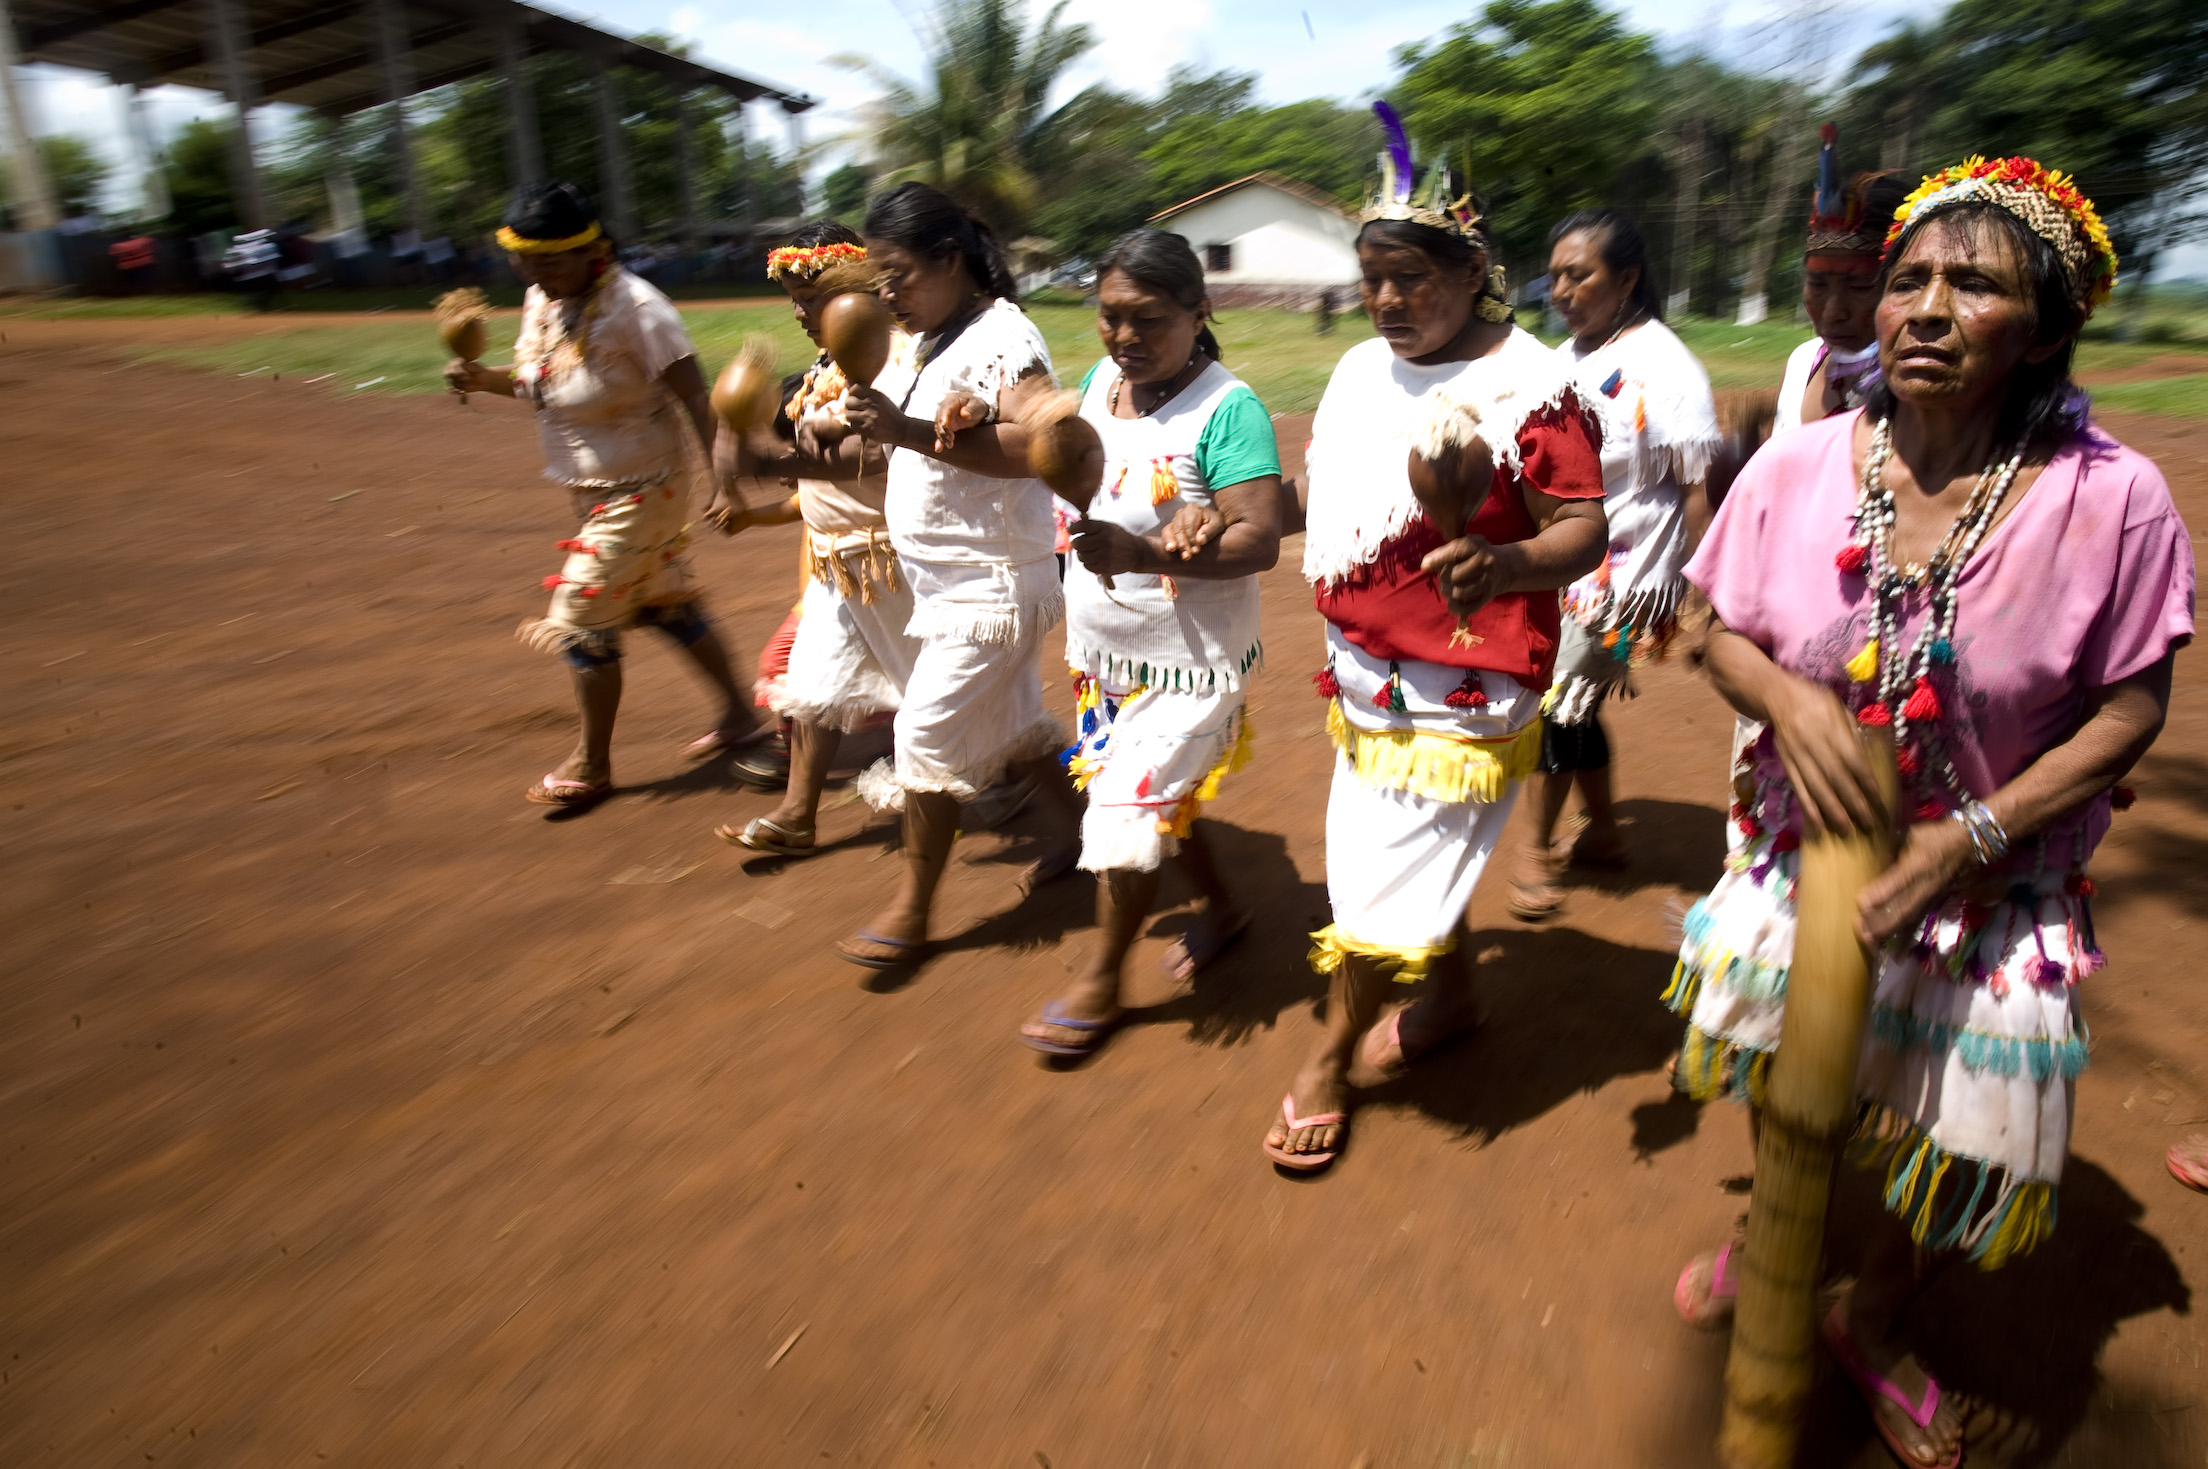
\includegraphics[width=4.752in,height=3.161in]{livroredesguaranifinal-img1.jpg}
 Mulheres Kaiow\'a e Guarani durante Aty Guasu, grande assembleia desses
povos, na Terra Ind\'igena Panambi-Lagoa Rica, em Douradina (MS). Foto:
Marcello Casal Jr. / Ag\^encia Brasil, 2012.

\section[Aguyjevete pra quem luta! A Comiss\~ao Yvyrupa e a busca por
nosso espa\c{c}o de viver]{Aguyjevete pra quem luta! A Comiss\~ao
Yvyrupa e a busca por nosso espa\c{c}o de viver}
 Tup\~a (Marcos dos Santos)\footnote{* Coordenador tenonde da Comiss\~ao
Guarani Yvyrupa.}

Eu sou Tup\~a e meu nome em portugu\^es \'e Marcos. O trabalho que
fa\c{c}o com o meu povo na Comiss\~ao Guarani Yvyrupa aprendi com meus
pais, grandes l\'ideres, e com os xeram\~oi, os caciques aqui de S\~ao
Paulo e no litoral. Eu sou nascido no Rio Silveira, em Bertioga, e me
criei na aldeia Boa Vista, em Ubatuba. Na d\'ecada de 1980, os
xeram\~oi lutaram pelo reconhecimento das terras na faixa litor\^anea.
Nessa \'epoca, eles se referiam muito ao jaguata, que \'e o nosso
caminhar, a mobilidade guarani. Em todas essas \'areas na faixa
litor\^anea, desde o Rio Grande do Sul at\'e Esp\'irito Santo, os
grandes l\'ideres lutavam pela perman\^encia nessas aldeias, porque era
muito forte o n\~ao reconhecimento delas pelos que falavam que eram
donos dessas terras. 

Meu pai me levava nos encontros de aldeia em aldeia e em reuni\~oes
junto com o governo, com a Funai. Nesses encontros eu aprendi a luta do
movimento guarani. 

Foi muito forte ver a dificuldade deles por n\~ao falarem bem o
portugu\^es, n\~ao saberem escrever, n\~ao saberem ler. Ent\~ao eu me
interessei em estar junto com eles, ajudando. E me espelhei muito nas
duas lideran\c{c}as que acompanhavam nossos xeram\~oi, que foi o meu
tio Manoel e o finado Valdelino, da aldeia da Barragem [Tenonde
Por\~a]. Eles eram os porta-vozes desses grandes caciques. Os Guarani
falavam nhandepy [na nossa l\'ingua] nas reuni\~oes. Mesmo na cidade,
junto com os secret\'arios, com a Funai, os l\'ideres falavam em
Guarani nessa luta, ent\~ao eram esses dois Guarani que falavam em
portugu\^es para os representantes do governo. Em v\'arias reuni\~oes,
na hora de assinar a ata, o registro dos jurua, o pessoal simplesmente
carimbava o seu dedo, e apenas os jurua escreviam. Isso me chamou muito
a aten\c{c}\~ao, e tamb\'em a import\^ancia desse trabalho de
tradu\c{c}\~ao que eles faziam.

Na \'epoca, a gente que acompanhava os mais velhos ia mais pra brincar,
vivia correndo pra l\'a e pra c\'a, n\~ao prestava muita aten\c{c}\~ao
nas reuni\~oes. Depois \'e que fomos vendo que a gente deveria se
inteirar dos assuntos e come\c{c}ar a acompanhar a discuss\~ao deles.
Isso foi em 1984, 1985... Conversamos que cada aldeia poderia organizar
um movimento de jovens. Da\'i tomei a iniciativa de fazer isso na minha
aldeia, Boa Vista [em Ubatuba/SP]. Tamb\'em tinha o mais velho que era
o xondaro da aldeia, o guardi\~ao que ensinava a parte da
organiza\c{c}\~ao interna da aldeia, nas ro\c{c}as, no plantio, fazia
as casas, a limpeza no terreno. E fui ent\~ao junto com ele, auxiliando
na aldeia, e esse grupo de jovens virou depois a associa\c{c}\~ao da
comunidade.

Registramos a Associa\c{c}\~ao e, como eu estava movimentando os jovens,
fui eleito o presidente. Tivemos uma proposta de escola junto com a
prefeitura municipal, e o CTI [Centro de Trabalho Indigenista] nos
ajudou nessa \'epoca. Tinha um Guarani que se formou na cidade, estudou
um pouco e depois lecionou pra n\'os. Nesse contexto aprendi a parte de
alfabetiza\c{c}\~ao na escola da aldeia. Depois eu fiz uma pequena
parte de estudo na cidade tamb\'em. N\~ao me formei por causa do
trabalho junto com os jovens na minha aldeia e depois em outras
aldeias, na Barragem, no Rio Silveira... Ent\~ao foi surgindo essa
ideia de ampliar a participa\c{c}\~ao dos jovens na quest\~ao
pol\'itica.

Eu acompanhei o trabalho dos nossos caciques junto com o pessoal do CTI,
do CIMI [Centro Indigenista Mission\'ario] e dos demais apoiadores.
Conseguimos o reconhecimento das terras Guarani na faixa litor\^anea,
que foi na aldeia Boa Vista, no Rio Silveira, na aldeia do Rio Branco,
Itariri e nas tr\^es aldeias aqui na capital. S\~ao pequenas terras que
foram conseguidas com grande luta, pois foi uma press\~ao muito forte. 

Apesar do reconhecimento dessas terras ser pequeno, n\'os vimos que
t\'inhamos que enfrentar a situa\c{c}\~ao. Participamos de encontros em
que fal\'avamos da presen\c{c}a guarani na faixa litor\^anea e tamb\'em
no nosso territ\'orio yvy mbyte, que \'e o centro da terra, como os
nossos mais velhos falam, na regi\~ao do Paraguai e Argentina. Tem todo
o contexto da mobilidade Guarani, da busca da Terra sem Mal, yvy mara
e{\textquoteright}\~{y}, em que os Guarani vieram ocupando espa\c{c}os.
Tamb\'em teve nossa xejaryi que faleceu na aldeia do Esp\'irito Santo,
Maria Tatax$\iota [342?]$, ela teve essa caminhada em busca de yvy mara
e{\textquoteright}\~{y} e fundou aldeias em S\~ao Paulo e no Rio de
Janeiro. Mas onde os Guarani chegavam, ocupavam uma certa regi\~ao e
a\'i chegava um tal dono, e os Guarani n\~ao s\~ao de conflito, ent\~ao
simplesmente se retiravam daquele local, iam pra outros lugares e a\'i
foram perdendo territ\'orio. Fomos conversando sobre tudo isso nos
encontros.

Conhecendo mais sobre a minha hist\'oria, desde a \'epoca da
coloniza\c{c}\~ao, ou da ocupa\c{c}\~ao dos jurua, da coloniza\c{c}\~ao
portuguesa, vi que se n\'os simplesmente f\^ossemos saindo das aldeias,
a gente ia ficar sem terra. Ia chegar um momento em que n\'os
ter\'iamos que enfrentar e lutar pelos nossos direitos. Ent\~ao
participei tamb\'em, l\'a em Bras\'ilia, do movimento pelos direitos
ind\'igenas na Constitui\c{c}\~ao de 88. Nesse contexto fui me formando
na quest\~ao Guarani, da minha lideran\c{c}a interna da aldeia e
tamb\'em me fortalecendo, adquirindo conhecimentos na quest\~ao
pol\'itica atual.

A organiza\c{c}\~ao dos caciques de 1984 a 1989 se chamava AGUAI,
{\textquotedblleft}A\c{c}\~ao Guarani Ind\'igena{\textquotedblright},
aqui em S\~ao Paulo. Cheguei a ser presidente nessa organiza\c{c}\~ao,
mas, por dificuldades financeiras e de n\~ao conseguir apoio, tivemos
que fech\'a-la. Tamb\'em tivemos outras organiza\c{c}\~oes do nosso
jeito, sem ser registrado, mas a gente sempre caminhou na luta, na
defesa dos direitos. A\'i vimos que cada lideran\c{c}a em cada estado
fazia seu movimento separado, sem muita aproxima\c{c}\~ao. Tinham as
lideran\c{c}as no Esp\'irito Santo, no Rio de Janeiro, em S\~ao Paulo,
Paran\'a, Santa Catarina, Rio Grande do Sul... Ent\~ao n\'os fomos nos
juntando, conversando com os mais velhos, com os xeram\~oi, buscando
mais informa\c{c}\~oes, mais instrumentos de luta. Junto com eles,
n\'os vimos que era importante ter uma representa\c{c}\~ao nossa, dos
Guarani do Sul e do Sudeste. Tivemos ent\~ao v\'arios encontros,
reuni\~oes, e a\'i tivemos em 2006 uma reuni\~ao em Sete Barras, quando
formamos uma representa\c{c}\~ao Guarani do Sul e do Sudeste, com a
representa\c{c}\~ao de cada lideran\c{c}a que estava se destacando nos
estados. Formamos a comiss\~ao Guarani Yvyrupa nesse contexto. 

Pra n\'os a terra \'e uma s\'o, n\~ao se limita por estado, por
munic\'ipio, nessas divisas pol\'iticas. Nhanderu, nosso deus, criou,
gerou essa terra pra todos os povos viverem, nesse conceito. Tamb\'em
politicamente n\'os acompanhamos a discuss\~ao l\'a em Bras\'ilia, com
o movimento nacional, com a APIB, que \'e a Articula\c{c}\~ao dos Povos
Ind\'igenas do Brasil, e todas as reuni\~oes que eles fazem convidam a
Comiss\~ao Guarani Yvyrupa.

Ultimamente estamos acompanhando de perto a discuss\~ao sobre os
territ\'orios ind\'igenas e as propostas de mudan\c{c}a que est\~ao
ocorrendo em Bras\'ilia. Isso pra n\'os \'e muito preocupante porque
nesse contexto atual \'e o governo que executa a demarca\c{c}\~ao das
terras, a Funai, o Minist\'erio da Justi\c{c}a e a Presid\^encia da
Rep\'ublica que homologa a terra. Nesse processo j\'a tem muita
dificuldade, porque os tais
{\textquotedblleft}propriet\'arios{\textquotedblright} entram na
Justi\c{c}a, muitas terras s\~ao judicializadas e n\~ao conseguimos com
mais rapidez ter a garantia das nossas terras. E hoje, com as PECs que
est\~ao a\'i no Congresso, esse processo pode ser transferido para o
poder legislativo, que \'e o prop\'osito da bancada ruralista. Eles
est\~ao se organizando, e t\^em poder econ\^omico da grande pecu\'aria
e dos plantadores de soja. 

N\'os estamos nos organizando tamb\'em, procurando buscar apoio com
nossos amigos, parceiros, entidades e ONGs. Est\'a sendo dif\'icil hoje
a discuss\~ao l\'a em Bras\'ilia, e isso se reflete muito nas terras
ind\'igenas do Mato Grosso do Sul e n\'os aqui na faixa litor\^anea na
Mata Atl\^antica. Essa est\'a sendo a maior discuss\~ao hoje no
momento. Em toda a faixa litor\^anea, desde o Rio Grande do Sul at\'e
Santa Catarina, h\'a tamb\'em terras que foram reconhecidas como
compensa\c{c}\~ao dos impactos ambientais, da constru\c{c}\~ao ou da
duplica\c{c}\~ao de ferrovias, que s\~ao adquiras por compra. Essas
terras s\~ao pequenas, \`as vezes com 50, 100 hectares, e a\'i acaba
sendo um outro formato de reconhecimento.

Temos o reconhecimento da ocupa\c{c}\~ao tradicional pelo artigo 231 e
hoje corre o risco desse artigo ser mudado para o reconhecimento ter
que passar pelo Congresso Nacional, do Poder Legislativo. Tivemos uma
manifesta\c{c}\~ao aqui na rodovia dos Bandeirantes da aldeia do
Jaragu\'a. Junto com os nossos parceiros, n\'os organizamos a
mobiliza\c{c}\~ao dos Guarani aqui em S\~ao Paulo, na Avenida Paulista.
Eu tive que ir a Bras\'ilia pra acompanhar o movimento nacional l\'a,
que teve a representa\c{c}\~ao de todos os povos do Brasil. Fizemos
manifesta\c{c}\~oes na regi\~ao do centro de Bras\'ilia, no Supremo
Tribunal, em frente ao Pal\'acio da Presid\^encia da Rep\'ublica e do
ministro da Justi\c{c}a. Houve momentos tensos, em que todos os povos
se organizaram no acampamento para ir at\'e o Congresso, onde foram
barrados pelos policiais. O povo Kayap\'o e Xavante, outros povos que
estavam juntos se dirigindo at\'e o Pal\'acio Nacional, foram barrados
pelos policiais, que tamb\'em jogaram spray de pimenta. Mas algumas
partes do Poder Executivo formalmente se posicionaram contra a PEC 215,
o projeto de lei 227 e outras PECs que est\~ao sendo discutidas pela
comiss\~ao especial que estava sendo instalada. A vice-presidente da
c\^amara disse que essa comiss\~ao n\~ao podia ter continuidade.

Em uma manifesta\c{c}\~ao geral dos povos ind\'igenas, estivemos
tamb\'em no Supremo Tribunal conversando com um dos representantes, o
relator assessor, sobre a portaria 303 e as dezenove condicionantes
para a demarca\c{c}\~ao de terras. Essa portaria est\'a sendo usada
pelos contr\'arios \`as demarca\c{c}\~oes, especialmente no Mato
Grosso. S\~ao todas essas quest\~oes que n\'os enquanto movimento
ind\'igena, enquanto movimento da Comiss\~ao Guarani Yvyrupa, estamos
articulando, acompanhando junto com o movimento nacional.

A nossa luta enquanto movimento Guarani \'e a demarca\c{c}\~ao das
terras. Estamos tamb\'em acompanhando em toda a regi\~ao a quest\~ao
dos empreendimentos que impactam as terras ind\'igenas, como a
constru\c{c}\~ao ou duplica\c{c}\~ao de rodovia, constru\c{c}\~ao de
barragem, hidrel\'etrica, enfim, todas essas quest\~oes que v\^em
afetar as terras ind\'igenas. Ent\~ao \'e um movimento muito tenso em
Bras\'ilia, que est\'a refletindo em todas as terras ind\'igenas no
Brasil.

Tenho muito orgulho do meu povo, fa\c{c}o parte da comunidade e, nesse
movimento, estamos organizando tamb\'em a Comiss\~ao Mirim, que s\~ao
os jovens que est\~ao nos acompanhando na discuss\~ao. A cada
reuni\~ao, evento, encontro ou assembleia, est\~ao participando os
jovens. Esse \'e meu papel, formar essa nova gera\c{c}\~ao assim como
fui formado pelos mais velhos. 

Aguyjevete: agradecimento e plenitude a todos que est\~ao nessa luta!

\section[Carta veiculada pela Comiss\~ao Yvyrupa por ocasi\~ao da tinta
vermelha no Monumento \`as Bandeiras ]{Carta veiculada pela Comiss\~ao
Yvyrupa por ocasi\~ao da tinta vermelha no Monumento \`as Bandeiras }
  [Warning: Image ignored] % Unhandled or unsupported graphics:
%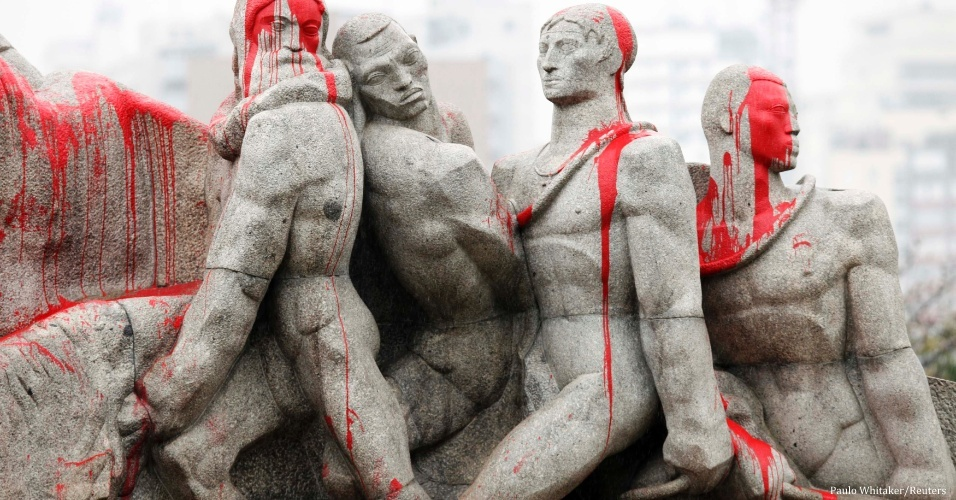
\includegraphics[width=3.428in,height=1.7925in]{livroredesguaranifinal-img2.jpg}
 

Para n\'os, povos ind\'igenas, a pintura n\~ao \'e uma agress\~ao ao
corpo, mas uma forma de transform\'a-lo. N\'os, da Comiss\~ao Guarani
Yvyrupa, organizac[327?]\~ao pol\'itica aut\^onoma que articula o povo
guarani no sul e sudeste do pa\'is, realizamos no \'ultimo dia 02 de
outubro, na Av. Paulista, a maior manifesta\c{c}\~ao ind\'igena que
j\'{a} ocorreu em S\~ao Paulo desde a Confederac\~ao dos Tamoios. Mais
de quatro mil pessoas ocuparam a Av. Paulista, sendo cerca de
quinhentas delas dos nossos parentes, outros duzentos de comunidades
quilombolas e mais de tr\^es mil apoiadores n\~ao-ind\'igenas, que
viram a for\c{c}a e a beleza do nosso movimento. Muitos meios de
comunica\c{c}\~ao, por\'em, preferiram noticiar nossa
manifesta\c{c}\~ao como se tivesse sido uma depreda\c{c}\~ao de algo
que os brancos consideram ser uma obra de arte e um patrim\^onio
p\'ublico. 

Saindo da Av. Paulista, marchamos em dire\c{c}\~ao a essa est\'atua de
pedra, chamada de Monumento \`as Bandeiras, que homenageia aqueles que
nos massacraram no passado. L\'a subimos com nossas faixas, e hasteamos
um pano vermelho que representa o sangue dos nossos antepassados, que
foi derramado pelos bandeirantes, dos quais os brancos parecem ter
tanto orgulho. Alguns apoiadores n\~ao-ind\'igenas entenderam a
for\c{c}a do nosso ato simb\'olico, e pintaram com tinta vermelha o
monumento. Apesar da cr\'itica de alguns, as imagens publicadas nos
jornais falam por si s\'o: com esse gesto, eles nos ajudaram a
transformar o corpo dessa obra ao menos por um dia. Ela deixou de ser
pedra e sangrou. Deixou de ser um monumento em homenagem aos genocidas
que dizimaram nosso povo e transformou-se em um monumento \`a nossa
resist\^encia. Ocupado por nossos guerreiros xondaro, por nossas
mulheres e crianc[327?]as, esse novo monumento tornou viva a bonita e
sofrida hist\'oria de nosso povo, dando um grito a todos que queiram
ouvir: que cesse de uma vez por todas o derramamento de sangue
ind\'igena no pa\'is! Foi apenas nesse momento que esta est\'atua
tornou-se um verdadeiro patrim\^onio p\'ublico, pois deixou de servir
apenas ao simbolismo colonizador das elites para dar voz a n\'os
ind\'igenas, que somos a parcela origin\'aria da sociedade brasileira.
Foi com a mesma inten\c{c}\~ao simb\'olica que travamos na semana
passada a Rodovia dos Bandeirantes, que al\'em de ter impactado nossa
Terra Ind\'igena no Jaragu\'a, ainda leva o nome dos assassinos.

A tinta vermelha que para alguns de voc\^es \'e depreda\c{c}\~ao j\'a
foi limpa e o monumento ja voltou a pintar como her\'ois, os genocidas
do nosso povo. Infelizmente, por\'em, sabemos que os massacres que
ocorreram no passado contra nosso povo e que continuam a ocorrer no
presente n\~ao terminaram com esse ato simb\'{o}lico e n\~ao ir\~ao
cessar t\~ao logo. Nossos parentes continuam esquecidos na beira das
estradas no Rio Grande do Sul. No Mato Grosso do Sul e no Oeste do
Paran\'a continuam sendo cotidianamente ameac[327?]ados e assassinados
a mando de pol\'iticos ruralistas que, com a coniv\^encia silenciosa do
Estado, roubam as terras e a dignidade dos que sobreviveram aos ataques
dos bandeirantes. Tamb\'em em S\~ao Paulo esse massacre continua, e
perto de voc\^es, vivemos confinados em terras min\'usculas, sem
condi\c{c}\~oes m\'inimas de sobreviv\^encia. Isso sim \'e vandalismo.

Ficamos muito tristes com a rea\c{c}\~ao de alguns que acham que a
homenagem a esses genocidas \'e uma obra de arte, e que vale mais que
as nossas vidas. Como pode essa est\'atua ser considerada patrim\^onio
de todos, se homenageia o genoc\'idio daqueles que fazem parte da
sociedade brasileira e de sua vida p\'ublica? Que tipo de sociedade
realiza tributos a genocidas diante de seus sobreviventes? Apenas
aquelas que continuam a pratic\'a-lo no presente. Esse monumento para
n\'os representa a morte. E para n\'os, arte \'e a outra coisa. Ela
n\~ao serve para contemplar pedras, mas para transformar corpos e
esp\'iritos. Para n\'os, arte \'e o corpo transformado em vida e
liberdade e foi isso que se realizou nessa intervenc[327?]\~{a}o.

Aguyjevete pra todos que lutam! -- Tup\~a (Marcos dos Santos)

A caminho do Sol: cosmografias guarani

Daniel Calazans Pierri\footnote{* Mestre pelo PPGAS-USP e membro do
Centro de Trabalho Indigenista (CTI).}

Isso que eu tenho pra contar. Ent\~ao, n\'os Guarani ir\'iamos nos
encontrar frente a frente com os brancos. Nhanderu [divindade criadora
do universo] j\'a nos destinou para sermos tekoaxy [seres terrestres
com corpo perec\'ivel], nos destinou para caminhar entre o lugar onde
Nhamandu [divindade solar] se po[1EBD?] e o fim da terra dele
[yvyrak\~a]. Por isso, seguindo o caminho de Nhamandu viemos. \'E por
isso que at\'e hoje estamos aqui. Os primeiros viveram no centro da
terra [yvy mbyte] e vieram seguindo o caminho de Nhamandu porque assim
\'e o caminho que a alma das crian\c{c}as faz, elas v\^em desde onde o
sol nasce, mandadas pelos deuses para confiar e se concentrar neles.
Isso tudo j\'a acontecia desde antes do brancos estarem aqui, j\'a
v\'inhamos para a beira do mar. Ent\~ao, os brancos n\~ao deveriam nem
perguntar porque vivemos aqui. N\'os j\'a sabemos disso tudo pelos
nhamandu kuery [coletividade dos Nhamandu], porque seguimos o caminho
deles e em todo esse percurso formamos as nossas aldeias, na
dire\c{c}\~ao da morada de Nhanderu. Aqueles que vivem pra onde o sol
se po[1EBD?] [A morada de Tup\~a], eles est\~ao em contato com quem
est\'a aqui, porque eles tamb\'em caminham at\'e pela beira do mar. 

Os brancos usaram a nossa l\'ingua para dar o nome a todas as coisas que
tem nesse territ\'orio: as cidades, os rios, todas as coisas est\~ao na
nossa l\'ingua. S\'o isso j\'a serviria como uma prova da nossa
presen\c{c}a, como dizem os brancos. N\~ao tem como dizer que n\~ao
estivemos sempre por aqui pois seria mentira! A gente vai falar que \'e
mentira pois sabemos a verdade. Tamb\'em tem as tava [ru\'inas], que
eram usadas pelos Guarani. S\~ao as ru\'inas, como dizem os brancos:
como elas existiriam por toda parte desse territ\'orio se n\~ao fosse
porque os Guarani passaram por a\'i? 

Se n\~ao existisse o Guarani aqui n\~ao existiriam essas ru\'inas. Tinha
aldeias grandes mesmo antigamente, bem perto de onde \'e o Rio de
Janeiro. L\'a perto tinha 17 aldeias. Em 1500, quando os brancos
passaram, os Guarani n\~ao queriam entregar as suas aldeias e por isso
os brancos mataram muitos. S\~ao Paulo tamb\'em \'e a mesma coisa,
tinha aldeia grande bem perto de onde \'e a cidade. Tudo isso
aconteceu, mas como os brancos n\~ao querem dar a terra para n\'os e
eles s\~ao maioria, eles n\~ao querem contar a verdade. Mesmo assim, a
gente vai vencer porque a gente tem a sabedoria dos nhanderu kuery
[coletivo gen\'erico das divindades]. At\'e aqui foi a minha palavra,
aqui na Aldeia Peguaoty, que vai ser uma aldeia mesmo, bem grande.

(Cacique Lu\'is Eus\'ebio -- dia 30/01/2011, na Aldeia Peguaoty -- Sete
Barras, litoral do Estado de S\~ao Paulo)

Essa narrativa, da qual reproduzo apenas um pequeno trecho, foi
realizada na l\'ingua guarani no contexto de um estudo para a
regulariza\c{c}\~ao da Terra Ind\'igena onde se insere a aldeia na qual
vive o autor da narrativa. Trata-se de uma aldeia do povo Mbya-Guarani,
povo esse que ocupa uma s\'erie de fragmentos de um vasto territ\'orio,
que atinge desde a regi\~ao litor\^anea do Brasil, nos Estados de
Esp\'irito Santo, Rio de Janeiro, S\~ao Paulo, Paran\'a, Santa Catarina
e Rio Grande do Sul, passando pelo interior desses quatro \'ultimos
Estados e se espalha pela regi\~ao oriental do Paraguai, e pela
prov\'incia de Missiones, na Argentina.

Construiu-se em parte da literatura antropol\'ogica especializada e,
sobretudo, em parte da chamada {\textquotedblleft}opini\~ao
p\'ublica{\textquotedblright} a ideia de que os Guarani-Mbya seriam um
povo {\textquotedblleft}origin\'ario do Paraguai ou da
Argentina{\textquotedblright} que realizou migra\c{c}\~oes desesperadas
para o litoral apenas recentemente, inspirado por um movimento
messi\^anico sem futuro. Todavia, existe documenta\c{c}\~ao hist\'orica
que comprove a presen\c{c}a dos Guarani-Mbya no litoral brasileiro,
desde ao menos a segunda metade do s\'eculo XIX, e nada na
documenta\c{c}\~ao permite afirmar com seguran\c{c}a que esse povo
esteve ausente do litoral em qualquer momento do per\'iodo
colonial.{\textquotedblright}

Sem entrar nesse debate, cabe enfatizar que a narrativa acima representa
um esfor\c{c}o evidente de mobilizar parte do arsenal cosmol\'ogico de
que disp\~oe o narrador para argumentar no sentido de defender seu
direito \`a demarca\c{c}\~ao da terra e de se contrapor a aquela
vis\~ao acerca das origens dos Guarani-Mbya. Trata em parte, portanto,
de uma mobiliza\c{c}\~ao pol\'itica de uma narrativa m\'itica. Tamb\'em
por isso (e nunca apesar disso) a mesma narrativa apresenta uma s\'erie
de elementos important\'issimos e complexos para uma compreens\~ao do
que seriam as concep\c{c}\~oes cosmol\'ogicas dos Guarani Mbya a
respeito do espa\c{c}o terrestre habitado, de sua cosmografia e de
aspectos importantes de sua cosmog\^enese.

Esse \'e o tema central deste texto, que pretende lan\c{c}ar luz sobre a
riqueza dessas concep\c{c}\~oes a respeito do  espa\c{c}o terrestre, 
abordando a maneira atrav\'es da qual elas s\~ao mobilizadas no
discurso das lideran\c{c}as na defesa de seus direitos territoriais.
Tratarei de tr\^es conceitos nativos relacionados, todos eles
mobilizados direta ou indiretamente nessa disputa: yvyrupa (cuja
tradu\c{c}\~ao literal \'e plataforma terrestre); yvy mbyte (centro do
mundo) e yvy apy ou yvy ak\~a (extremidade do mundo, ou fim da terra).
Os tr\^es conceitos aparecem no discurso acima, mas pretendo
principalmente contribuir para uma melhor compreens\~ao do conceito de
yvyrupa, porque esse foi o nome escolhido para a mais importante
organiza\c{c}\~ao supralocal dos Mbya: a Comiss\~ao Guarani Yvyrupa,
sobre a qual falarei brevemente ao concluir o texto.

Mas voltemos antes para o relato, para sua refer\^encia central. O
cacique Luis Eus\'ebio desconstr\'oi a id\'eia mobilizada pelos seus
advers\'arios de que os Guarani Mbya n\~ao seriam origin\'arios do
litoral. Para tanto, esclarece que os Guarani s\~ao descendentes
diretos de Nhamandu, o Sol, que \'e uma das principais divindades do
pante\~ao guarani. 

Entretanto, para compreender o que dizia Luis Eus\'ebio \'e preciso
conhecer uma outra narrativa, muito contada entre os Guarani, que \'e
uma variante daquela que a literatura antropol\'ogica convencionou
chamar o {\textquotedblleft}mito dos g\^emeos{\textquotedblright}.
Segundo ela, Nhamandu, o Sol, nasceu na primeira terra, yvy tenonde,
onde o seu pai, criador do universo, Nhanderu Tenonde Papa, esteve e
fecundou magicamente uma mulher que aqui vivia, Nhandexy. Ao se
desentender com ela, Nhanderu partiu de volta \`a sua morada celeste,
que ficava a leste. Toda a hist\'oria \'e narrada como um percurso que
\'e seguido por Nhamandu, o Sol, desde que estava no ventre de sua
m\~ae, \`a procura da morada celeste de seu pai, Nhanderu. No meio da
narrativa, sua m\~ae \'e devorada por on\c{c}as, e ap\'os esse
epis\'odio Sol cria Jaxy, o Lua, para lhe fazer companhia como um
irm\~aozinho. Ao fim, eles s\~ao recebidos de volta na morada de
Nhanderu Tenonde, o pai deles, que se situa em uma plataforma celeste
localizada ao leste.

Essa narrativa, que \'e uma das principais da cosmog\^enese desse povo,
tem para os Mbya uma territorialidade muito marcada. O Sol ainda na
barriga da m\~ae, percorre a plataforma terrestre partindo do local que
eles concebem como sendo o centro do mundo (yvy mbyte) e segue em
dire\c{c}\~ao ao leste at\'e que atinge, j\'a com seu irm\~ao Lua, o
fim da terra (yvy ak\~a). Ap\'os o fim da terra havia nesse tempo uma
outra ilha (yy pa\~u), \`a qual passam Kuaray e Jaxy, matando as
on\c{c}as origin\'arias. Essa outra ilha, que vai se separando
progressivamente da terra, tornar-se-\'a uma das moradas celestes, e
esse processo de separa\c{c}\~ao desemboca na cria\c{c}\~ao do mar. 

Era justamente a essa narrativa dos irm\~aos Sol e Lua que o cacique
Luis Eus\'ebio se referia para dizer  que os Guarani
{\textquotedblleft}foram destinados a andar do centro do mundo ao fim
da terra{\textquotedblright}. Quando ele dizia que os primeiros viviam
no centro da terra e vieram {\textquotedblleft}seguindo o caminho de
Nhamandu{\textquotedblright}, h\'a dois sentidos a se extra\'ir da\'i.
Em primeiro lugar, deve-se entender que os primeiros s\~ao justamente
Sol e Lua, Nhamandu e Jaxy, divindades que os Guarani do mundo
terrestre atual consideram seus antepassados e \`as quais est\~ao
destinados a imitar. Em segundo lugar, esse mesmo caminho \'e pensado
tamb\'em como qualquer trajeto percorrido na dire\c{c}\~ao do sol
nascente, ao leste, onde se situa a morada de Nhanderu Tenonde.

O movimento do pr\'oprio astro solar tamb\'em \'e recorrentemente
abordado pelos meus interlocutores. Dizem os Guarani que Nhamandu, o
Sol, sai todo dia de sua morada ao leste iluminando a terra com um
aparelho de luz e depois o desliga e faz novamente o percurso de volta,
o mesmo que fez quando esteve na plataforma terrestre, do centro da
terra ao leste.

Mas o discurso de Lu\'is Eus\'ebio, ao deixar impl\'icitas essas
quest\~oes, fala explicitamente de suas decorr\^encias na vida concreta
dos Guarani. Ele diz que {\textquotedblleft}em todo esse percurso
sempre formamos as nossas aldeias, na dire\c{c}\~ao da morada de
Nhanderu.{\textquotedblright} Ou seja, ele indica os preceitos
cosmol\'ogicos que delimitam o territ\'orio de ocupa\c{c}\~ao dos
Guarani. Estando os Guarani destinados a
{\textquotedblleft}imitar{\textquotedblright} os her\'ois da ra\c{c}a,
como dizia Alfred Metraux, eles devem formar suas aldeias em toda a
extens\~ao do percurso que foi realizado no in\'icio dos tempos pelos
irm\~aos Sol e Lua, abrangendo desde a regi\~ao central do mundo, que
eles identificam ao Paraguai e \`a regi\~ao fronteir\'i\c{c}a deste
pa\'is com Argentina e Brasil, at\'e a extremidade do mundo, que \'e a
regi\~ao litor\^anea do Brasil. E se foi assim na primeira terra com os
antepassados divinos dos Guarani, os her\'ois Sol e Lua, sempre foi
assim ao longo da hist\'oria: {\textquotedblleft}mesmo antes da chegada
dos brancos{\textquotedblright}, como diz Luis Eus\'ebio,
{\textquotedblleft}j\'a est\'avamos na beira do
mar{\textquotedblright}.

Entende-se, assim, que a id\'eia mobilizada pelos setores contr\'arios
\`a demarca\c{c}\~ao das terras guarani no litoral guarda uma
conson\^ancia com a cosmologia guarani que n\~ao passa de um mal
entendido. Da mesma maneira que seus advers\'arios, os Guarani
consideram que seus primeiros antepassados viveram inicialmente no
local que eles consideram ser o centro do mundo, yvy mbyte, e que
coincide com alguma localidade no Paraguai, como veremos adiante. De
acordo com a sua cosmog\^enese, de fato {\textquotedblleft}vieram do
Paraguai{\textquotedblright}. Entretanto, os que vieram fizeram esse
percurso n\~ao nesse mundo atual, mas na primeira terra que foi
destru\'ida pelo dil\'uvio, saindo do centro do mundo at\'e a regi\~ao
do litoral, yvy apy, a extremidade do mundo. Foram os antepassados
m\'iticos Sol e Lua que delimitaram como territ\'orio de ocupa\c{c}\~ao
dos seus descendentes Guarani toda a regi\~ao onde hoje se estendem as
centenas de aldeias existentes.

Outra passagem da cosmogese Guarani \'e necess\'aria para compreender
sua concep\c{c}\~ao de espa\c{c}o. Muitos dizem que a primeira terra,
quando foi gerada por Nhanderu Tenonde, foi gerada sobre uma grande
\'agua, na forma de uma pequena ilha, que n\~ao tinha mais que o
tamanho da planta do p\'e de Nhanderu. Posteriormente, esta ilha foi
sendo ampliada e formou a terra, ou mais precisamente o continente
americano no tamanho que ele tem hoje. Esse local onde se iniciou a
terra \'e justamente esse centro do mundo, yvy mbyte, localizado
provavelmente onde hoje \'e o Paraguai.

O espa\c{c}o terrestre \'e chamado yvyrupa, termo cuja tradu\c{c}\~ao
literal \'e suporte ou plataforma terrestre. \'E dito suporte porque
\'e concebido como uma estrutura, dentre outras, que sustenta uma ilha
concebida como um amontoado de terra que existe em meio a um universo
feito de \'agua. A esse respeito, transcrevo um trecho de uma outra
narrativa realizada tamb\'em em guarani por um anci\~ao de outra aldeia
localizada numa ilha no litoral de S\~ao Paulo, pr\'oxima \`a aldeia do
autor da primeira narrativa:

\begin{quotation}
Esse mundo \'e grande. Em cima da terra tem um mar. E embaixo da terra
tem um mar muito grande. Embaixo da terra \'e s\'o \'agua. \'E tudo
\'agua, \'e mais \'agua que a terra. \'E desse mar, que Nhanderu pega
\'agua pra fazer chuva. E n\~ao \'e salgada. A \'agua que est\'a
embaixo dessa terra \'e maior que o mar que a gente v\^e. O mar que a
gente v\^e \'e pequeno comparado com esse que tem embaixo da terra. E
esse n\~ao \'e salgado.

(...)

Em cima da terra, aqui em cima, essa \'agua \'e salgada, j\'a est\'a
toda salgada. Mas embaixo, n\~ao \'e salgada. Ent\~ao, \'e da\'i que
ele pega \'agua pra fazer a chuva. Ent\~ao, por isso que tem a
nascente, essa que chega nas cachoeiras e nos rios, ela nunca vai
acabar. Elas v\^em diretamente debaixo da terra. V\^em desse mar
grande, que n\~ao salgado, \'e de l\'a que chega a nascente.

(...) 

J\'a contaram pra voc\^e sobre o centro da terra? No Paraguai? Yvy
mbyte. L\'a existe a amarra\c{c}\~ao da terra. \'E uma corda que sai do
centro da terra e atravessa at\'e outro mundo. De uma esp\'ecie de
gancho, ele atravessa para o outro mundo.

Porque existem quatro mundos. No quarto mundo est\'a Nhamandu. \'E a
corda do centro do mundo. Tem uma corda, que na verdade \'e um vento,
\'e um vento fino. E essa corda est\'a esticada. E o mundo l\'a fica
assim por isso, l\'a no centro da terra \'e mais alto. E pra c\'a ele
abaixa mais, e fica assim. E a corda passa para o outro mundo, tamb\'em
pelo meio. E l\'a \'e o centro do mundo. \'E o centro exato, l\'a no
Paraguai. Eu n\~ao fui, mas minha av\'o me contou.

\end{quotation}
Essa narrativa, como a primeira, apresenta uma s\'erie de elementos
complexos a respeito de elabora\c{c}\~oes cosmol\'ogicas realizadas
pelos Guarani, que n\~ao terei espa\c{c}o para abordar aqui (a esse
respeito, ver Pierri, 2013). Mas o que quero chamar aten\c{c}\~ao, \'e
que reecontramos um tema cl\'assico da literatura Guarani, desenvolvido
com detalhes n\~ao abordados por autores como Cadogan ou Curt
Nimuendaju, que lan\c{c}aria nova luz sobre as concep\c{c}\~oes guarani
a respeito do espa\c{c}o terrestre, de yvyrupa, como dizem os \'indios.
Nimuendaju foi o primeiro autor que j\'a pode ser considerado um
antrop\'ologo a testemunhar os chamados movimentos prof\'eticos
realizados por grupos guarani, saindo de regi\~oes interioranas para
atingir \`a chamada Terra Sem Mal. Como \'e sabido, ele dizia em suas
Lendas da cria\c{c}\~ao e destrui\c{c}\~ao do mundo (1987 [1914]) que
encontrou grupos guarani que sa\'iam do sul do Mato Grosso do Sul em
dire\c{c}\~ao ao litoral paulista, inspirados por l\'ideres xam\^anicos
para atingir em vida a morada dos deuses. Dizia tamb\'em, o que quase
nunca \'e notado, que embora os \'indios dissessem que a Terra Sem Mal
se situava al\'em do mar, {\textquotedblleft}a maioria a
leste{\textquotedblright}, alguns falavam {\textquotedblleft}de uma
outra Terra Sem Mal localizada no centro da terra{\textquotedblright}.

Ora, na narrativa que transcrevi acima, meu interlocutor nos esclarece
que existem quatro mundos, quatro plataformas, uma situada em cima da
outra, sendo a \'ultima delas a morada de Nhamandu, o Sol. Diz tamb\'em
que tanto embaixo como em cima dessa terra h\'a uma grande \'agua, h\'a
um mar, que n\~ao podemos ver. Desse modo, a plataforma terrestre,
yvyrupa, \'e concebida como uma estrutura que sustenta uma ilha, em
volta da qual h\'a mar por todos os lados, por cima e por baixo.
Levando isso em considera\c{c}\~ao, a diferencia\c{c}\~ao de Nimuendaju
entre uma Terra Sem Mal que seria localizada no centro da terra e outra
que estaria al\'em do mar, pode n\~ao fazer tanto sentido. Entre a
plataforma celeste e plataforma terrestre h\'a \'agua por todos os
lados. Portanto, para atingir a morada dos deuses, seja saindo do
litoral, na extremidade do mundo, ou do interior, no centro do mundo,
ser\'a preciso atravessar as \'aguas, o grande mar que a gente n\~ao
v\^e.

A partir dessa concep\c{c}\~ao, esse \'ultimo anci\~ao me explicava de
uma maneira muito peculiar o que pensava sobre algo que Nimuendaju
chamava de {\textquotedblleft}cren\c{c}a na destrui\c{c}\~ao do
mundo{\textquotedblright}, e que para esse autor tinha rela\c{c}\~ao
direta com o profetismo. Ele me dizia que a estrutura dessa terra atual
foi refor\c{c}ada depois da destrui\c{c}\~ao das \'ultimas tr\^es
terras que a precederam. Por isso, ela \'e segura e n\~ao vai acabar
nunca. Entretanto, Nhanderu Tenonde est\'a nervoso com a
devasta\c{c}\~ao promovida pelos brancos e vai limpar a terra. Com
isso, ele quer dizer que Nhanderu vai varrer toda a terra que existe em
cima de yvyrupa, da plataforma terrestre, e renovar tudo com terra
nova, destruindo a humanidade atual. O que n\~ao acaba, portanto, \'e a
estrutura terrestre, o suporte da terra. 

Percebe-se, logo, que o conceito guarani de yvyrupa \'e muito mais
literal do que poderia parecer. Refere-se de fato a uma estrutura que
sustenta a terra em que pisamos e que foi constru\'ida progressivamente
a partir do centro do mundo, onde ela est\'a amarrada a outras
estruturas que sustentam outros mundos.

Assim como vimos que Luis Eus\'ebio utilizava esses conceitos para
rebater argumentos de pessoas contr\'arias \`a demarca\c{c}\~ao de suas
terras, yvyrupa tornou-se, a partir das \'ultimas d\'ecadas, um termo
utilizado frequentemente por grandes parte das lideran\c{c}as
pol\'iticas guarani-mbya mobilizadas na luta por suas terras. Utilizam
esse conceito de yvyrupa com o mesmo prop\'osito que tinha Luis Eusebio
no discurso transcrito ao in\'icio, justamente para para justificar seu
direito \`a ocupa\c{c}\~ao de aldeias espalhadas pela regi\~ao mais
populosa do Brasil, al\'em de Paraguai e Argentina.

Na luta pol\'itica frente ao Estado Nacional, as lideran\c{c}as
Guarani-Mbya dizem: {\textquotedblleft}os mais velhos chamam nosso
territ\'orio de yvyrupa, e esse termo quer dizer que a terra \'e uma
s\'o. Yvyrupa significa mundo sem fronteiras.{\textquotedblright}

Embora seja uma tradu\c{c}\~ao que n\~ao d\'a conta da complexidade das
concep\c{c}\~oes de que tratamos apenas brevemente aqui, o bord\~ao
mobilizado a partir do conceito de yvyrupa resume boa parte das
implica\c{c}\~oes que essas concep\c{c}\~oes tem para o uso que eles
fazem do espa\c{c}o terrestre: grande mobilidade territorial,
ocupa\c{c}\~ao de espa\c{c}os fragmentados de um territ\'orio extenso,
anterioridade em rela\c{c}\~ao aos brancos e n\~ao reconhecimento das
fronteiras impostas pelos Estados-na\c{c}\~ao.

Em 2006, lideran\c{c}as guarani-mbya de grande parte das aldeias
situadas nos Estados de Esp\'irito Santo, Rio de Janeiro, S\~ao Paulo,
Paran\'a, Santa Catarina e Rio Grande do Sul, criaram em grande
assembl\'eia uma organiza\c{c}\~ao pol\'itica a qual denominaram
Comiss\~ao Guarani Yvyrupa. Ela se define pelo seu Estatuto como
{\textquotedblleft}uma organiza\c{c}\~ao ind\'igena guarani que foi
formada para defender os direitos territoriais, garantidos pela
Constitui\c{c}\~ao Federal e pelas conven\c{c}\~oes internacionais, e
os interesses coletivos do povo Guarani.{\textquotedblright} O mesmo
estatuto diz ainda que
{\textquotedblleft}{\textquoteleft}Yvyrupa{\textquoteright} significa
{\textquoteleft}leito da terra{\textquoteright} ou {\textquoteleft}a
terra \'e uma s\'o{\textquoteright}.{\textquotedblright}

A Comiss\~ao Guarani Yvyrupa formalizou um movimento que j\'a vinha
acontecendo desde da d\'ecada de 1980 em todo o litoral brasileiro,
quando as lideran\c{c}as das diversas aldeias da regi\~ao passaram a se
articular conjuntamente para lutar pela demarca\c{c}\~ao de suas
terras, que na maioria das vezes situam-se em fragmentos de Mata
Atl\^antica, rodeados por cidades, estradas, fazendas e diversos outros
empreendimentos instalados no processo de coloniza\c{c}\~ao do Brasil.

A utiliza\c{c}\~ao do conceito de yvyrupa como emblema desse movimento
pol\'itico \'e interessante porque se tratava justamente de um
movimento visando fazer com que as aldeias superassem o isolamento
territorial que foi imposto pelo Estado, reconhecendo sua luta comum
enquanto um povo \'unico.

Para isso, optaram por utilizar esse termo que denota em sua l\'ingua
todo o espa\c{c}o terrestre, onde vivem os Guarani, os brancos e uma
s\'erie de outros povos, como se significasse exclusivamente
{\textquotedblleft}territ\'orio guarani{\textquotedblright}. Yvyrupa
\'e o territ\'orio guarani, dizem. Embora seja uma aproxima\c{c}\~ao,
essa tradu\c{c}\~ao n\~ao deixa de denotar um aspecto central dessas
concep\c{c}\~oes que abordamos. A devasta\c{c}\~ao da Mata Atl\^antica
e de boa parte dos recursos naturais do planeta foi realizada pelos
brancos, resultando na expropria\c{c}\~ao do territ\'orio guarani.
Isso, como vimos, enervou as divindades, antepassados dos Guarani, e
elas pretendem por isso limpar a terra, acabando com todos que
estiverem aqui, \'indios e brancos. Afinal, {\textquotedblleft}a terra
\'e uma s\'o{\textquotedblright}. Estamos todos juntos em yvyrupa.

Refer\^encias

NIMUENDAJU, Curt Unkel. As lendas da cria\c{c}\~ao e destrui\c{c}\~ao do
mundo como fundamentos da religi\~ao dos Apapoc\'uva-Guarani. S\~ao
Paulo, Hucitec/Edusp, 1987 [1914].

PIERRI, Daniel Calazans. O perec\'ivel e o imperec\'ivel: l\'ogica do
sens\'ivel e corporalidade no pensamento guarani-mbya.
Disserta\c{c}\~ao de Mestrado. S\~ao Paulo: PPGAS-USP, 2013.

Desde o s\'eculo XVI os Guarani tiveram uma s\'erie de tradutores, uns
melhores, outros piores, mas muita gente fazendo um esfor\c{c}o de
compreender esse pensamento que eles nos apresentaram. As dificuldades
come\c{c}am ao tentarmos aplicar nossas categorias a esse pensamento.
Uma das quest\~oes \'e a natureza como separada daquilo que a gente
chamaria de cosmologia, religi\~ao, metaf\'isica, cultura, seja l\'a o
que for. N\~ao h\'a como separar. Mas por que a gente tem tanta
dificuldade em afirmar isso? Talvez porque ainda pensamos a natureza
como coisa a ser utilizada. Pierre Clastres foi um dos primeiros a
apontar que um dos problemas da expans\~ao capitalista \'e n\~ao deixar
o mundo \`a sua alegre improdutividade, sendo preciso faz\^e-lo servir
e render. Esse discurso est\'a o tempo todo rondando a briga ind\'igena
pelas terras, mas tamb\'em nossos conceitos. Felizmente algumas
pesquisas atuais tem nos proporcionado tradu\c{c}\~oes melhores,
falando mais nos termos guarani do que nos nossos. -- Beatriz
Perrone-Moys\'es

Novas terras sem males: a luta guarani-kaiowa pelos tekoha

Spensy K. Pimentel\footnote{* Docente na Universidade Federal do Sul da
Bahia. Este artigo amadureceu a partir de di\'alogos com o historiador
kaiowa Izaque Jo\~ao e o nhanderu Atan\'asio Teixeira, a quem
agrade\c{c}o imensamente pela oportunidade de di\'alogo. O presente
texto constitui um desdobramento de reflex\~oes iniciadas em Pimentel
(2012a), sobretudo a partir de uma entrevista, citada em ambos os
textos, que foi gravada com o sr. Atan\'asio para o v\'ideo
{\textquotedblleft}Mbaraka --- A Palavra que Age{\textquotedblright},
realizado em parceria com Edgar Teodoro da Cunha e Gianni Puzzo a
partir do pr\^emio Etnodoc 2009. Na tradu\c{c}\~ao das entrevistas para
o v\'ideo, agrade\c{c}o especialmente pelo apoio de Eliel Benites e
Graciela Chamorro.} 

Os Guarani-Kaiowa\footnote{ No contexto sul-matogrossense, os
Guarani-Kaiowa costumam usar a designa\c{c}\~ao
{\textquotedblleft}Kaiowa e Guarani{\textquotedblright}, diferenciando
os falantes do dialeto kaiowa e os do dialeto nhandeva --- localmente,
estes s\~ao denominados Guarani. Em outras regi\~oes, vale notar, o
jogo de etn\^onimos \'e distinto.} angariaram solidariedade nacional e
internacional nos \'ultimos anos em fun\c{c}\~ao da repercuss\~ao na
internet e meios de comunica\c{c}\~ao tradicionais das not\'icias sobre
a luta ferrenha e desigual que esse grupo ind\'igena trava pela
demarca\c{c}\~ao de suas terras na regi\~ao sul de Mato Grosso do Sul.

Desde os anos 1980, t\^em sido frequentes as den\'uncias envolvendo, por
um lado, mortes de lideran\c{c}as e despejos violentos em retomadas de
terra e, por outro, um cotidiano de fome, viol\^encia e suic\'idios nas
antigas reservas demarcadas pelo Servi\c{c}o de Prote\c{c}\~ao ao
\'Indio, as quais se encontram superlotadas e em p\'essimas
condi\c{c}\~oes pol\'iticas, econ\^omicas e sociais (Pimentel, 2010;
Pimentel \& Moncau, 2011).

Conhecido como Aty Guasu --- Grande Assembleia Kaiowa e Guarani, esse
movimento de luta pela terra envolve reuni\~oes peri\'odicas com
centenas de lideran\c{c}as, que costumeiramente divulgam uma
declara\c{c}\~ao final em portugu\^es. Antigamente entregues \`as
autoridades de \'org\~aos como Minist\'erio P\'ublico Federal e
Funda\c{c}\~ao Nacional do \'Indio (Funai), hoje, esses textos ganham
grande divulga\c{c}\~ao via internet.

E, pois, l\^e-se no documento final de uma recente Aty Guasu:

N\~ao vamos tolerar mais essa demora [nas demarca\c{c}\~oes de terra] e
vamos nos organizar cada vez mais para retomarmos nossas terras, custe
o que custar. E que o sangue de nosso povo semeie as nossas terras
sagradas para renascer a esperan\c{c}a de alcan\c{c}armos a terra sem
males (...)\footnote{ Documento final da Aty Guasu realizada na aldeia
Paso Piraju (Dourados-MS --- terra ind\'igena em processo de
identifica\c{c}\~ao), datado de 21/8/2011. Dispon\'ivel em
{\textless}http://twixar.me/N99{\textgreater}.}

N\~ao se trata de um exemplo \'unico. O uso do termo
{\textquotedblleft}terra sem males{\textquotedblright} \'e corriqueiro
nos documentos ligados \`as Aty Guasu. No discurso pol\'itico do
movimento, a associa\c{c}\~ao entre as \'areas a serem demarcadas e a
Terra sem Males \'e uma constante. O termo correspondente, em guarani,
\'e mesmo Yvy Marane{\textquoteright}y, algo simples de verificar no
di\'alogo com as lideran\c{c}as.

Como pensar, ent\~ao, essa Yvy Marane{\textquoteright}y \`a qual n\~ao
se chega a partir de uma longa caminhada at\'e a beira da plataforma
celeste, tal como boa parte da literatura etnol\'ogica em torno dos
Guarani desenvolveu ao longo do s\'eculo XX? Que terra sem males \'e
essa que se pode acessar rompendo a cerca dos latif\'undios
sul-matogrossenses?

Formam um denso emaranhado as associa\c{c}\~oes que os textos
etnol\'ogicos fizeram, ao longo do s\'eculo XX, em torno desse que se
tornou um dos grandes temas guarani, a Terra sem Males, Yvy
Marane{\textquoteright}y.

Noelli (1999) rememorava-nos o longo processo, por meio do qual se
teceram hip\'oteses cada vez mais abrangentes --- e arriscadas ---
sobre a Terra sem Males e, particularmente, sua associa\c{c}\~ao com a
mobilidade guarani. O autor destaca, na cria\c{c}\~ao do que chama de
{\textquotedblleft}mito acad\^emico{\textquotedblright} (1999: 123), as
obras de Nimuendaju (1987 [1914]) e M\'etraux (1927).

Em resumo: o pioneiro Nimuendaju encontra, em 1912, uma fam\'ilia
guarani dirigindo-se a p\'e para a Serra do Mar, no litoral atl\^antico
brasileiro. Eles --- que, ao que tudo indica, j\'a haviam viajado por
centenas de quil\^ometros rumo ao leste --- lhe dizem que fazem esse
caminho para tentar chegar, em vida, \`a Terra sem Males, yvy
marane{\textquoteright}y, um lugar {\textquotedblleft}onde n\~ao mais
se morre{\textquotedblright}. O autor elucubra: e se, de modo geral, as
migra\c{c}\~oes tupi-guarani anteriores \`a conquista fossem tamb\'em
uma busca por esse para\'iso terreal? (1987: 107).

A hip\'otese de Nimuendaju come\c{c}a a ser dada como favas contadas,
cresce mais e mais, sobretudo a partir de M\'etraux, que a
{\textquotedblleft}refor\c{c}a e amplifica{\textquotedblright}, na
avalia\c{c}\~ao de Noelli  (1999: 136). Talvez, o exemplo mais
significativo sobre a dimens\~ao que tomaram os imaginados
{\textquotedblleft}motivos religiosos{\textquotedblright} para os
movimentos coletivos guarani esteja na an\'alise que se construiu a
respeito do termo kandire.

Autores como Viveiros de Castro (1995: 247, 371) ou Pissolato (2007:
410-11) --- entre muitos outros, diga-se de passagem --- tomam, a
partir de H\'el\`ene Clastres (1978), certa glosa de Cadogan a respeito
da express\~ao o\~nemokandire, constante de um dos cantos mbya
compilados pelo autor no Ayvu Rapyta: descrever-se-ia, a\'i,
{\textquotedblleft}el tr\'ansito de la inmortalidad sin sufrir la
prueba de la muerte, es decir, la ascensi\'on al cielo despu\'es de
purificar el cuerpo mediante los ejercicios
espirituales{\textquotedblright} (Cadogan, 1997: 101). 

Tratar-se-ia, pois, de um elemento central no conjunto de ideias que
resultaria na proposta de Viveiros de Castro, com a no\c{c}\~ao de uma
{\textquotedblleft}ambival\^encia do humano{\textquotedblright}
(Pissolato, 2007: 410) posta em destaque nas cosmologias tupi-guarani.
Esse autor, como se sabe, considerava a ideia de um
{\textquotedblleft}modelo tupi-guarani{\textquotedblright} (1986:
623-700), elaborado a partir de uma compara\c{c}\~ao entre os Tupi
seiscentistas, os Guarani e os Arawet\'e --- bem como de alguns
paralelos com outros grupos tupi amaz\^onicos contempor\^aneos.

Em tal constructo, a {\textquotedblleft}metaf\'isica
tupi-guarani{\textquotedblright} envolvia uma concep\c{c}\~ao de pessoa
constitu\'ida pelo {\textquotedblleft}devir{\textquotedblright} (1986:
623). Entre os Guarani, especificamente, a concep\c{c}\~ao da pessoa
como devir se expressaria no aguyje, que consiste no ideal xam\^anico
de, por meio do aperfei\c{c}oamento corporal/espiritual, alcan\c{c}ar a
imortalidade/ {\textquotedblleft}amadurecimento{\textquotedblright}.
Viveiros de Castro recupera a\'i H\'el\`ene Clastres (1978), autora que
associava uma suposta passagem das migra\c{c}\~oes guarani documentadas
no s\'eculo XVI --- j\'a entendidas como uma procura da Terra sem Males
--- \`a ascese xam\^anica da busca pela perfei\c{c}\~ao individual, o
aguyje, capaz de levar a esse para\'iso em vida, como se tivesse
ocorrido um processo de
{\textquotedblleft}interioriza\c{c}\~ao{\textquotedblright} da busca
pela Yvy Marane{\textquoteright}y\footnote{ Essa configura\c{c}\~ao de
uma teoria guarani da pessoa, de fato, remonta ainda \`a obra de
Nimuendaju, que, em seu relato sobre a cren\c{c}a na duplicidade da
alma entre os Apapokuva (1987: 29-47), j\'a apontava para essa
{\textquotedblleft}vis\~ao dual da pessoa{\textquotedblright} (Viveiros
de Castro, 1987: xxvii).}.

Cadogan, nessa mesma passagem citada, indica, por\'em, um fato-chave.
{\textquotedblleft}Es sugestivo que a una naci\'on no guarani se haya
designado en la \'epoca de la conquista con este nombre Kandire. Se los
habr\'a considerado como inmortales por poseer una cultura
superior?{\textquotedblright} (Cadogan, 1997: 101). E, se, para al\'em
de um conceito relativo \`a cosmologia, tratava-se de um termo aplicado
a um ou mais grupos com o qual ou os quais os Guarani mantinham contato
e que, por sua cultura caracter\'istica, inspirava(m) essa
associa\c{c}\~ao, de quem se estaria falando?

Recentemente, Comb\`es e Julien s\~ao duas autoras que retornaram a esse
enigma dos Kandire, referidos nos documentos coloniais. Elas recuperam
uma s\'erie de documentos quinhentistas a respeito do deslocamento de
grupos de l\'ingua guarani ao longo da bacia do Prata, rumo \`a
regi\~ao do piemonte andino, nas proximidades do que hoje \'e Santa
Cruz de La Sierra, na Bol\'ivia, demonstrando evid\^encias de que,
longe de representar, simplesmente, uma {\textquotedblleft}rea\c{c}\~ao
\`a conquista{\textquotedblright}, essas movimenta\c{c}\~oes --- h\'a
muito conhecidas, mas ainda pouco estudadas --- indicam a exist\^encia
de uma grande rede de trocas, alian\c{c}as e hostilidades, implicando
um fluxo intenso de pessoas e bens, particularmente a presen\c{c}a de
objetos de metal andino circulando por toda a \'area. Ou seja, um
panorama bem menos compat\'ivel com a hip\'otese de
{\textquotedblleft}motivos religiosos{\textquotedblright}, ou
{\textquotedblleft}levantes pol\'itico-m\'isticos{\textquotedblright},
como sintetiza Julien (2007: 265).

As explica\c{c}\~oes para essa movimenta\c{c}\~ao guarani, segundo tal
autora, apontam muito mais para a busca por metais e a \^ansia por
resgatar parentes presos em expedi\c{c}\~oes anteriores --- o que, para
Julien, demonstra que, em vez de falar em migra\c{c}\~oes guarani rumo
aos Andes, seria mais produtivo perceber que se tratava de enormes
redes de alian\c{c}as e hostilidades, que inclusive ultrapassavam em
muito as barreiras lingu\'isticas (idem: 251, 254).

Nesse contexto, como aparece o termo kandire? As autoras demonstram que,
em v\'arios documentos, trata-se mesmo de um grupo, n\~ao um lugar ---
os Kandire\footnote{ Nos documentos e, por conseguinte, nos textos de
Comb\`es e Julien, \'e frequente que se grafe o termo como Candire ---
aqui, usarei genericamente kandire, adequando-se \`a grafia utilizada
no guarani contempor\^aneo. }, portanto, como j\'a percebia Cadogan
---, e que o termo se referiria aos Inca. Seriam os
{\textquotedblleft}se\~nores verdaderos del metal
amarillo{\textquotedblright}, ou seja, o ouro (Comb\`es, 2011: 102).
Mais precisamente, Comb\`es argumenta que as men\c{c}\~oes aos Kandire
se refeririam aos Inca da regi\~ao de Samaipata --- fortaleza
constru\'ida para defender minas de prata exploradas pelos andinos na
regi\~ao pr\'oxima a Santa Cruz. Os Carcaraes, outro grupo tamb\'em
citado nos documentos, seriam mitimaes (funcion\'arios) empregados pelo
inca Condori nessas minas conhecidas como Saypuru --- a pr\'opria
designa\c{c}\~ao Kandire poderia ser derivada de Condori, sup\~oe
(2011: 102-3).

A autora busca refinar as hip\'oteses de Julien --- n\~ao \'e que se
deva opor os {\textquotedblleft}motivos religiosos{\textquotedblright}
de Nimuendaju a um c\'alculo e uma raz\~ao {\textquotedblleft}\`a
ocidental{\textquotedblright}, que justifica a movimenta\c{c}\~ao
registrada na bacia do Prata a partir de motiva\c{c}\~oes materiais.
{\textquotedblleft}Una {\textquotesingle}tierra rica{\textquotesingle}
de metal bien puede a la vez ser tierra de {\textquotesingle}cosas
buenas{\textquotesingle}{\textquotedblright}, conjectura ela (2011:
103-4).

Comb\`es lembra que M\'etraux j\'a apontava para uma converg\^encia
entre as buscas pela m\'itica Terra sem Males e os Inca --- da mesma
forma que Saignes percebia que esses movimentos tinham algo a ver com a
busca por metais. Mais recentemente, isso n\~ao passou despercebido a
autores como Monteiro (1992) e Carvalho (1992), mas o fato \'e que
n\~ao se tiraram consequ\^encias pr\'aticas da exist\^encia desses
dados para a caracteriza\c{c}\~ao dos coletivos ind\'igenas que atuam
na hist\'oria da regi\~ao, bem como de seus movimentos e redes de
circula\c{c}\~ao.

O que est\'a em jogo aqui \'e a oposi\c{c}\~ao cartesiana entre sagrado
e profano, ou entre raz\~ao pr\'atica e raz\~ao simb\'olica. Tudo era
concomitante, e n\~ao havia contradi\c{c}\~ao nisso.
{\textquotedblleft}En cuanto a la b\'usqueda del metal andino, se trata
al parecer de un af\'an demasiado
{\textquotesingle}materialista{\textquotesingle} para caber en la
imagen idealizada de un para\'iso terrenal{\textquotedblright}, ironiza
Comb\`es, em outro texto (2011b: 27).

As viagens guarani rumo ao Oeste (sejam migra\c{c}\~oes ou
expedi\c{c}\~oes) s\~ao um tema pouco explorado na bibliografia
etnol\'ogica sobre os Guarani. Men\c{c}\~oes a elas s\~ao feitas, mas
sem maiores detalhes sobre suas motiva\c{c}\~oes\footnote{ Veja-se, por
exemplo, Meli\'a, Gr\"unberg e Gr\"unberg, (2008: 16-7), ou Meli\'a
(1993). Mesmo quando se menciona essa quest\~ao, como em Monteiro
(1992: 484), pode parecer que os grupos guarani simplesmente seguiam os
europeus que buscavam o metal. }. A discuss\~ao cl\'assica, em geral
projetada ao passado, oscilou entre considerar as antigas
migra\c{c}\~oes tupi-guarani como {\textquotedblleft}crises
messi\^anicas{\textquotedblright} (M\'etraux, 1979: 175), oriundas da
{\textquotedblleft}acultura\c{c}\~ao{\textquotedblright}, com a chegada
dos europeus, ou, nas obras de Pierre e H\'el\`ene Clastres, como um
{\textquotedblleft}processo aut\'octone{\textquotedblright},
relacionado ao crescimento demogr\'afico\footnote{ Gloso aqui a leitura
que Pissolato (2007: 99-105) faz desse debate. Sztutman, por sua vez,
rejeita o termo {\textquotedblleft}messianismo{\textquotedblright}, mas
continua centrando a discuss\~ao no
{\textquotedblleft}profetismo{\textquotedblright} como
{\textquotedblleft}xamanismo feito hist\'oria{\textquotedblright}
(2005: 410) ou {\textquotedblleft}leitura da
hist\'oria{\textquotedblright} (op.cit.: 430) feita pelos povos
ind\'igenas. No caso chiriguano, ele foca sua an\'alise na obra de
Saignes a respeito da hist\'oria do grupo desde o per\'iodo colonial e
a emerg\^encia dos profetas tumpa, que se contrapunham aos mburuvicha. 
} e consequente expans\~ao geogr\'afica, que acirraria uma
{\textquotedblleft}contradi\c{c}\~ao entre o pol\'itico e o
religioso{\textquotedblright} (H. Clastres, 1978: 45): grandes chefes
com prest\'igio em escala cada vez maior, esp\'ecie de
{\textquotedblleft}for\c{c}a centr\'ipeta{\textquotedblright}, enquanto
os profetas agiriam de forma
{\textquotedblleft}centr\'ifuga{\textquotedblright}, numa a\c{c}\~ao
{\textquotedblleft}contra o Estado{\textquotedblright}, utilizando a
express\~ao de Pierre Clastres\footnote{ E por essa passagem se percebe
que H. Clastres tamb\'em percebia essa ambiguidade citada por Comb\`es,
entre {\textquotedblleft}raz\~oes ecol\'ogicas e
econ\^omicas{\textquotedblright} e {\textquotedblleft}raz\~oes de ordem
m\'itica{\textquotedblright} (H. Clastres, 1978: 59).}.

O problema que est\'a posto aqui \'e o seguinte: ser\'a mesmo que,
quando estamos falando de Terra sem Males, nos referimos a algo que
est\'a no polo do divino, do religioso, de um {\textquotedblleft}n\~ao
ser social{\textquotedblright}, de {\textquotedblleft}for\c{c}as
negadoras do social{\textquotedblright} (H. Clastres, 1978: 45), ou,
como afirmou, mais recentemente, Sztutman, de uma
{\textquotedblleft}tradu\c{c}\~ao guarani do devir n\~ao
humano{\textquotedblright} (Sztutman, 2005: 41)?

No Brasil, os Kaiowa e Guarani de Mato Grosso do Sul representam a
maioria absoluta dos atuais grupos de l\'ingua guarani. Eram, em 2013,
46,3 mil pessoas, habitando 30 terras ind\'igenas e cerca de outros 35
acampamentos --- muitos em beira de estrada, alguns dentro de fazendas
ocupadas para pressionar contra a morosidade na demarca\c{c}\~ao de
terras\footnote{ Os dados de popula\c{c}\~ao s\~ao da Secretaria
Especial de Sa\'ude Ind\'igena (Sesai). Afora os Guarani Kaiowa de Mato
Grosso do Sul, h\'a, no Brasil, outros 12,5 mil Guarani, de acordo com
a mesma fonte. A informa\c{c}\~ao sobre os acampamentos foi recolhida
pelo Conselho Indigenista Mission\'ario, em 2011. As terras
ind\'igenas, note-se, n\~ao est\~ao todas completamente ocupadas ---
h\'a casos em que os ind\'igenas esperam pela resolu\c{c}\~ao de
conflitos judiciais em apenas uma pequena por\c{c}\~ao da terra j\'a
demarcada, ou mesmo homologada (vide os casos Nhanderu Marangatu e
Arroio Kor\'a, que aguardam, h\'a anos, por decis\~oes do Supremo
Tribunal Federal).} ---, al\'em da periferia de cidades da regi\~ao.

Essa popula\c{c}\~ao conforma, hoje, o segundo maior grupo ind\'igena do
Brasil\footnote{ Se considerados em conjunto com os grupos guarani de
outros estados, estamos falando do maior povo ind\'igena do pa\'is, com
aproximadamente 58.800 pessoas (Sesai 2012a).} --- e o maior povo
ind\'igena fora da Amaz\^onia ---, mas tem \`a sua disposi\c{c}\~ao
pouco menos de 50 mil hectares de terra, efetivamente. H\'a algo em
torno de 40 mil hectares, aproximadamente, j\'a reconhecidos como
terras de ocupa\c{c}\~ao tradicional, mas ainda em poder de
fazendeiros, em fun\c{c}\~ao de arrastadas disputas judiciais. 

Desde 2008, ap\'os anos de press\~ao do Minist\'erio P\'ublico Federal,
a Funda\c{c}\~ao Nacional do \'Indio iniciou um processo, ainda
inconcluso, para identificar e delimitar como terras guarani-kaiowa
outras 39 \'areas, pelo menos, as quais, numa estimativa inicial,
somariam algo em torno de 600 mil hectares\footnote{ Atualmente,
trava-se uma pesada discuss\~ao sobre como se poder\'a efetivar a posse
dessas terras para os ind\'igenas, pois grande parte das \'areas est\'a
ocupada por fazendeiros que det\^em t\'itulos de terra concedidos,
d\'ecadas atr\'as, pelos governos federal ou estadual. Cf. Pimentel,
2010 e 2012; Pimentel \& Moncau, 2011.  }. 

Cada uma dessas \'areas pleiteadas pelos Kaiowa e Guarani \'e conhecida
como tekoha --- significando algo como {\textquotedblleft}o lugar onde
se pode viver do nosso pr\'oprio jeito{\textquotedblright}. Da forma
como \'e usado hoje, o termo \'e uma objetiva\c{c}\~ao que surgiu no
\^ambito das discuss\~oes sobre a demarca\c{c}\~ao de terras, desde os
anos 80. 

Do lado paraguaio, Meli\`a, Gr\"unberg e Gr\"unberg (2008) tinham
registrado o uso do termo no \^ambito do debate sobre a
regulariza\c{c}\~ao de terras pa\~\i{}-tavyter\~a\footnote{
Autodenomina\c{c}\~ao mais comum dos ind\'igenas falantes de kaiowa que
vivem do lado paraguaio.}, ocorrido por l\'a sobretudo nos anos 1970. A
despeito disso, como se sabe, palavras correlatas s\~ao muito comuns,
n\~ao s\'o na hist\'oria guarani (vide a obra de Montoya), como em
outros povos de l\'inguas tupi-guarani. Por exemplo, Gallois (2004)
registra, entre os Zo{\textquoteright}e, coletivo tupi amaz\^onico do
noroeste do Par\'a, contatado nos anos 1980, a emerg\^encia do termo
zo{\textquoteright}e rekoha, aplicado \`a Terra Ind\'igena
Zo{\textquoteright}e, durante o processo de reconhecimento territorial
pelo qual o grupo passou. 

No contexto atual, em Mato Grosso do Sul, o termo tekoha indica uma
por\c{c}\~ao de territ\'orio com o qual um determinado coletivo kaiowa
ou guarani consegue identificar uma rela\c{c}\~ao que pode ser
interpretada pelos n\~ao ind\'igenas como de
{\textquotedblleft}ocupa\c{c}\~ao tradicional{\textquotedblright}, ao
mesmo tempo em que percebe, ali, os elementos necess\'arios para
restabelecer o chamado teko por\~a, o bom modo de ser, o modo de ser
dos antigos, fugindo \`as m\'as condi\c{c}\~oes que imperam nas antigas
reservas demarcadas pelo SPI, onde --- sobretudo em fun\c{c}\~ao de se
viver {\textquotedblleft}misturado{\textquotedblright} (jopara) com os
karai (na proximidade das cidades) e da falta de alegria
(vy{\textquoteright}a) resultante da mis\'eria (por sua vez
relacionada, sobretudo, \`a superlota\c{c}\~ao e os problemas
ambientais) --- impera um teko vai (modo de ser ruim, ou imperfeito).

Essa forma de orientar a luta contra a coloniza\c{c}\~ao guarda forte
continuidade com outros momentos hist\'oricos entre grupos guarani. O
esfor\c{c}o dos xam\~as kaiowa e guarani, hoje, como h\'a v\'arios
s\'eculos, \'e o de pregar a volta ao nhande reko, seu modo pr\'oprio
de ser, de agir. {\textquotedblleft}Pegar o jeito do
branco{\textquotedblright}, uma express\~ao comum de se ouvir, \'e o
perigo. O nhande reko, o jeito kaiowa/guarani de ser, de fazer as
coisas, est\'a intimamente ligado \`as pr\'aticas xam\^anicas. Retomar
as \'areas de tekoha \'e recuperar h\'abitos e pr\'aticas dos antigos,
hoje impossibilitadas pelo ambiente (cada vez mais) urbano das grandes
reservas.

Essas pr\'aticas dos antigos, justamente, dependem de elementos que
n\'os designamos por {\textquotedblleft}natureza{\textquotedblright}.
Nesse sentido, mais uma vez, h\'a uma rela\c{c}\~ao direta entre a luta
pela terra, o xamanismo e a pol\'itica. Terra, aqui, \'e muito mais do
que o mero suporte para a
{\textquotedblleft}produ\c{c}\~ao{\textquotedblright} que nela veem os
brancos. De todo modo, o fato \'e que o projeto, teoria ou filosofia
kaiowa da pol\'itica passa, de forma decisiva, por aquilo que chamamos
de natureza. E isso n\~ao apenas no sentido
{\textquotedblleft}rom\^antico{\textquotedblright} identificado pelos
fazendeiros, de uma {\textquotedblleft}volta \`a
natureza{\textquotedblright}\footnote{ Esse termo \'e constantemente
evocado pelo establishment ruralista em MS para questionar o sentido do
movimento ind\'igena de luta pela terra (cf. Pimentel, 2012a e
2012b).}. Mais que um objetivo, a natureza \'e aliada no processo de
luta pela terra (cf. Pimentel, 2013).

Animais, plantas, elementos do clima (como ventos e raios) e da paisagem
(morros, rios, lagos) que servem como morada para certos seres, s\~ao
considerados manifesta\c{c}\~oes deles ou s\~ao elas mesmas entidades
participantes da luta pela terra. A forma mais gen\'erica de denominar
essas {\textquotedblleft}entidades sens\'iveis{\textquotedblright} (De
La Cadena, 2008), que s\~ao aliados, parentes, ou mesmo ancestrais dos
Kaiowa e Guarani \'e, como se viu, Tekoj\'ara, os
{\textquotedblleft}donos do nosso modo de ser{\textquotedblright}, numa
das poss\'iveis tradu\c{c}\~oes. Nesse sentido, o que est\'a em jogo,
na luta pela terra, \'e a expectativa de voltar a ocupar um espa\c{c}o
onde possam relacionar-se, da forma apropriada, com todos esses
seres-elementos citados (cf. Pereira, 2004).

A ideia de abandonar a ordem imposta pelos brancos e retomar os
{\textquotedblleft}antigos costumes{\textquotedblright}, ou os costumes
pr\'oprios, como fundamento das rebeli\~oes tupi e guarani, \'e
reiteradamente citada em documentos coloniais e, evidentemente,
transformada ao longo da hist\'oria, persiste at\'e os dias atuais.
Significativamente, por\'em, dan\c{c}ar e cantar continuam sendo atos
fundamentais na retomada dos {\textquotedblleft}bons
costumes{\textquotedblright} (teko por\~a), e subversivos aos olhos de
boa parte dos brancos da regi\~ao onde habitam, tal como nos tempos do
profeta Ober\'a, que liderou uma rebeli\~ao guarani em 1579 (cf.
Meli\'a, 1993).

O pensamento de um dos expoentes do movimento Aty Guasu, o
nhanderu\footnote{ Um dos termos mais comuns que os Kaiowa costumam
usar para designar os xam\~as --- {\textquotedblleft}nosso
pai{\textquotedblright}. No litoral, entre os Mbya/Nhandeva, designa o
Criador do Mundo. Para diferenciar os xam\~as deste personagem, os
Kaiowa chamam-no Nhanderuvusu --- {\textquotedblleft}nosso pai
maior{\textquotedblright}.} Atanasio Teixeira, \'e exemplar no sentido
de aclarar de que forma os tekoha s\~ao pensados como yvy
marane{\textquoteright}y. Al\'em de gozar de grande credibilidade como
curador e de ser considerado hoje um dos poucos conhecedores de
diversos rituais que j\'a n\~ao s\~ao mais realizados na maior parte do
territ\'orio kaiowa/guarani do lado brasileiro, em fun\c{c}\~ao da
degrada\c{c}\~ao ambiental, Atan\'asio \'e um nhanderu de extrema
import\^ancia na constru\c{c}\~ao do movimento de luta pela terra. 

Nos anos 1980, ele e outro xam\~a, o guarani Delosanto Centuri\'on,
morto em 2009, foram as principais figuras em um momento hist\'orico
decisivo: diante de uma s\'erie de impasses no processo de
regulariza\c{c}\~ao das terras ent\~ao reivindicadas, entre 1985 e
1986, eles passaram a criticar a forma como agiam as lideran\c{c}as que
ent\~ao estavam \`a proa das a\c{c}\~oes de luta.

Para eles, era preciso retomar o modo antigo de encaminhar a
resolu\c{c}\~ao dos problemas, cantando e dan\c{c}ando para pedir a
ben\c{c}\~ao e o apoio dos deuses, orientando o movimento de luta pela
terra de acordo com as instru\c{c}\~oes recebidas no processo de
di\'alogo xam\^anico com essas entidades\footnote{ Para um debate sobre
o princ\'ipio cosmopol\'itico que embasa essas formula\c{c}\~oes, a
ideia de que o xam\~a ideal \'e aquele que v\^e o futuro, recebendo a
denomina\c{c}\~ao de johexak\'ary, ver Pimentel (2012: cap. 3).}. Nesse
per\'iodo, os dois, junto com outros xam\~as, conseguiram apoio do
movimento ind\'igena para promover, a partir de 1987, as chamadas
Jeroky Guasu (grandes dan\c{c}as/rezas). Foi a partir dessa fase que
surgiu, pouco depois, o formato que \'e verificado at\'e hoje para as
assembleias Aty Guasu (cf. Pimentel, prelo).

At\'e hoje, Atan\'asio participa ativamente do movimento Aty Guasu, e
sua voz \'e ouvida com extrema defer\^encia nas assembleias. Em uma
entrevista com ele realizada em 2010\footnote{ Para o v\'ideo
{\textquotedblleft}Mbaraka: a palavra que age{\textquotedblright} ---
{\textless}https://vimeo.com/34768557{\textgreater}. O texto final da
tradu\c{c}\~ao deve-se especialmente a Eliel Benites e Graciela
Chamorro.}, assim se referia ao que ir\'a acontecer quando os Kaiowa e
Guarani conseguirem ocupar efetivamente as terras que hoje reivindicam:

Ent\~ao, haver\'a dan\c{c}a e caminhada at\'e o lugar onde vai renascer
a nossa terra, e \'e ali que n\'os vamos. Ali haver\'a novamente os que
v\~ao dan\c{c}ar, v\~ao ser arrumadas as casas. Ent\~ao, nesse lugar
eles v\~ao aben\c{c}oar, trazer coisas boas. Depois de aben\c{c}oar o
lugar, eles [os Nhanderu] v\~ao poder trazer de volta as nossas
ca\c{c}as, o dono da ca\c{c}a vai chamar os animais, eles v\~ao baixar
de novo.

As festas kaiowa e guarani, segundo a mem\'oria dos mais velhos, estavam
relacionadas a um tempo de fartura, antes do desmatamento massivo na
regi\~ao e do confinamento, quando as colheitas eram abundantes, e as
fam\'ilias podiam convidar periodicamente os vizinhos para cantar,
dan\c{c}ar e pedir aos deuses por sua sa\'ude e a alegria. Esses
rituais, como a nomina\c{c}\~ao das crian\c{c}as (nimongarai) ou a
passagem dos meninos \`a idade adulta (mit\~a pepy), sinalizada
antigamente por um furo na parte inferior da boca, o tembekua, onde se
instalava um fio de resina de certa \'arvore, o tembeta --- est\~ao
entre as mais fortes lembran\c{c}as de Atan\'asio, e comp\~oem o
cen\'ario da terra almejada, onde os parentes um dia poder\~ao voltar a
viver do seu pr\'oprio jeito, o nhande reko:

Ent\~ao haver\'a novamente o convite \`a cerim\^onia das crian\c{c}as
[mit\~a pepy], haver\'a novamente a celebra\c{c}\~ao do tembekua,
haver\'a novamente a dan\c{c}a [jerosy], o canto longo [mborahei puku],
pra trazer de volta a festa do milho verde [avati kyry]. V\~ao ser
aben\c{c}oados [hovasa] os canaviais, os mandiocais, as crian\c{c}as.
Vamos ter novamente ali todas as coisas, o novo lugar vai ser
fortalecido com as rezas, ali n\~ao ser\'a mais preciso ter outro modo
de viver. Ali haver\'a uma nova vida com dan\c{c}as, vida sadia, e vida
em abund\^ancia.

Como se pode ver, a descri\c{c}\~ao feita por Atan\'asio desse cen\'ario
de abund\^ancia que se aguarda para o momento de recupera\c{c}\~ao das
terras se aproxima muito da que se costuma fazer no contexto do
movimento ind\'igena. Os tekoha, portanto, s\~ao cen\'ario de uma
promessa de fartura, alegria e festa. O discurso pol\'itico, aqui, como
j\'a destacamos alhures (Pimentel, 2012b), se torna uma esp\'ecie de
profecia, uma vez que, no pensamento pol\'itico kaiowa e guarani, a
presen\c{c}a dos xam\~as nas a\c{c}\~oes coletivas \'e um dos fatores
determinantes para o sucesso de qualquer empreitada. \'E o xam\~a quem
deve dar o aval definitivo para qualquer movimenta\c{c}\~ao expressiva
de um coletivo, ou, caso contr\'ario, haver\'a s\'erios riscos de
fracasso. 

\'E nesse sentido que parece ser cada vez mais adequado deslocar a
discuss\~ao sobre o xamanismo guarani, que, n\~ao poucas vezes, foi
encaminhada para o campo da religi\~ao\footnote{ Deve-se fazer a
seguinte ressalva: no contexto local, para os pr\'oprios ind\'igenas,
ainda costuma ser bastante relevante discutir a quest\~ao do xamanismo
como op\c{c}\~ao religiosa, em fun\c{c}\~ao da persegui\c{c}\~ao
ferrenha que sofrem os nhanderu e nhandesy e seus familiares, por
parte, sobretudo, das igrejas evang\'elicas pentecostais --- as quais
se contam \`as dezenas, em \'areas como a de Dourados. }. \'E oportuno,
pensar a\'i no que vem sendo escrito sobre a ideia de
cosmopol\'itica\footnote{ Cosmopol\'itica seria a
{\textquotedblleft}nova pol\'itica{\textquotedblright}, no dizer de
Latour (2001: 347) --- a pol\'itica livre do acordo moderno que isolava
a natureza, como se a ela n\~ao dissessem respeito as decis\~oes
pol\'iticas. Por si s\'o, esse acordo j\'a definia um
{\textquotedblleft}cosmos{\textquotedblright} para uma certa
pol\'itica. Novos cosmos, novas pol\'iticas.}, ou
{\textquotedblleft}pol\'itica ontol\'ogica{\textquotedblright}, como
aponta Mol: 

A combina\c{c}\~ao dos termos
{\textquotedblleft}ontologia{\textquotedblright} e
{\textquotedblleft}pol\'itica{\textquotedblright} sugere-nos que as
condi\c{c}\~oes de possibilidade n\~ao s\~ao dadas \`a partida. Que a
realidade n\~ao precede as pr\'aticas banais nas quais interagimos com
ela, antes sendo modelada por essas pr\'aticas. (Mol, 2008: 63)

O deslocamento que propomos nos parece \'util no sentido de desfazer um
equ\'ivoco recorrente: enquanto tantos estiveram endossando os
{\textquotedblleft}motivos religiosos{\textquotedblright} das
migra\c{c}\~oes guarani hist\'oricas\footnote{ Somente Meli\'a (1989)
ousou levar \`as \'ultimas consequ\^encias essa discuss\~ao, sugerindo
o que, aqui, estamos constatando operar plenamente na atualidade: a
associa\c{c}\~ao entre a {\textquotedblleft}terra
ideal{\textquotedblright} e a terra almejada, disputada e conquistada
aqui mesmo, neste mundo.}, Atan\'asio e a Aty Guasu nos lembram que
essas dimens\~oes est\~ao, como parecem sempre ter estado,
completamente mescladas, que n\~ao \'e poss\'ivel separ\'a-las.
Diferente do que percebe H. Clastres para os Tupinamb\'a seiscentistas,
n\~ao se trata de um choque entre {\textquotedblleft}raz\~oes
econ\^omicas{\textquotedblright} e {\textquotedblleft}raz\~oes
m\'iticas{\textquotedblright}: os vetores se refor\c{c}am, n\~ao se
op\~oem.

Igualmente, na bibliografia a respeito dos Guarani do litoral, diversos
autores enfatizaram, nas \'ultimas d\'ecadas, a motiva\c{c}\~ao
originalmente {\textquotedblleft}religiosa{\textquotedblright} das
migra\c{c}\~oes guarani. Diante da persist\^encia, em certos segmentos
sociais, da ideia de que os ind\'igenas eram
{\textquotedblleft}invasores paraguaios{\textquotedblright},
amea\c{c}ando as \'areas de conserva\c{c}\~ao na Serra do Mar,
antrop\'ologos que identificavam uma
{\textquotedblleft}resist\^encia{\textquotedblright} em reconhecer a
rela\c{c}\~ao dessas migra\c{c}\~oes guarani com o tema da Terra sem
Males e a reprodu\c{c}\~ao dos caminhos trilhados pelos
{\textquotedblleft}grandes her\'ois
{\textquoteleft}divinizados{\textquoteright}{\textquotedblright}
(Ladeira, 2007: 66), lograram demonstrar que essa dimens\~ao
prof\'etica das migra\c{c}\~oes permanecia viva na mem\'oria de muitos
idosos. 

Em MS, como no litoral, trata-se, portanto, de reconhecer que as
dimens\~oes pol\'itico- territoriais e cosmol\'ogicas est\~ao
imbricadas. Em ambos os casos, pois, emerge uma discuss\~ao que
poder\'iamos caracterizar como cosmopol\'itica.

H\'a uma tend\^encia, contudo, que se deveria evitar, para que o
deslocamento cosmopol\'itico se efetive. Diante de apontamentos como os
de Noelli, supracitados, Chamorro tamb\'em reconhece a necessidade de
que se sublinhem as dimens\~oes s\'ocio-hist\'oricas ligadas ao tema da
Terra sem Males. {\textquotedblleft}Tanto as causas do medo da
destrui\c{c}\~ao do mundo s\~ao eventos s\'ocio-hist\'oricos como a
busca de uma {\textquoteleft}terra sem males{\textquoteright} n\~ao \'e
necessariamente uma fuga da realidade terrena para as esferas celestes,
pois \'e tamb\'em a busca de uma terra t\~ao real quanto
necess\'aria{\textquotedblright}, diz ela (Chamorro, 2010: 102). 

A quest\~ao \'e que ela remete a rela\c{c}\~ao aqui apontada a um campo
pol\'itico muito espec\'ifico, o das utopias: {\textquotedblleft}As
utopias e os mitos n\~ao dizem respeito s\'o ao mundo espiritual e os
acontecimentos hist\'orico-sociais s\~ao a base da dimens\~ao
transcendente da religi\~ao{\textquotedblright} (idem). Chamorro n\~ao
foi a \'unica a utilizar o termo
{\textquotedblleft}utopia{\textquotedblright} associado \`a Terra sem
Males. Carneiro da Cunha e Viveiros de Castro (2009[1985]: 95)
igualmente o fizeram. 

Por que, afinal, \'e que, mesmo quando reconhecemos a dimens\~ao
pol\'itica da Terra sem Males, vamos consider\'a-la uma
{\textquotedblleft}utopia{\textquotedblright}? Utopia, afinal --- assim
como mito ---, \'e um termo associado ao improv\'avel, ao sonho, \`a
fantasia. No Mato Grosso do Sul de hoje, \'e frequente que os
fazendeiros e seus apoiadores (na pol\'itica, na imprensa) se refiram
desse modo \`as pretens\~oes dos ind\'igenas de recuperarem suas terras
de ocupa\c{c}\~ao tradicional. Imaginar que poder\~ao transformar
aquelas \'areas hoje completamente desmatadas e est\'ereis em
planta\c{c}\~oes e florestas onde se recuperar\'a a biodiversidade e o
modo de vida dos antigos \'e imposs\'ivel, dizem os que se op\~oem aos
Kaiowa e Guarani.

Pode ser que o complexo de ideias em torno da Yvy
Marane{\textquoteright}y tenha apresentado tal sentido em alguma de
suas transforma\c{c}\~oes registradas ao longo destes cinco s\'eculos,
mas o fato \'e que, hoje, em Mato Grosso do Sul, s\~ao as terras a
serem demarcadas, os tekoha, que se tornaram a aut\^entica Terra sem
Males a que almejam os Kaiowa e Guarani, literalmente alcan\c{c}\'avel
pela a\c{c}\~ao pol\'itica planejada e consciente, e o \'unico
horizonte que muitos desses ind\'igenas vislumbram para que se possa
recuperar uma sociabilidade minimamente aceit\'avel, que proporcione
uma vida plenamente humana.

Diante dessas constata\c{c}\~oes, resta-nos, penso, refletir sobre o
sentido dessa nossa recusa a reconhecer como devir humano essa
esp\'ecie de movimento pol\'itico --- pois, afinal, \'e em
condi\c{c}\~oes absolutamente subumanas que os Kaiowa e Guarani t\^em
sido obrigados a sobreviver nas \'ultimas d\'ecadas\footnote{ E isso,
em suas pr\'oprias palavras: \'e comum, no \^ambito do movimento Aty
Guasu, que as lideran\c{c}as comparem a situa\c{c}\~ao dos Kaiowa e
Guarani nas reservas com a de porcos presos num chiqueiro.}. Por que
\'e que esse tipo de movimento fica confinado, na bibliografia, ao
campo do religioso, da utopia?

Um recente debate, justamente, nos ajuda a pensar a respeito disso. Em
2008, o ent\~ao ministro da Secretaria de Assuntos Estrat\'egicos,
Mangabeira Unger, foi questionado, em entrevista\footnote{ Publicada em
O Globo, 27/5/2008.}, se achava que os \'indios j\'a n\~ao teriam terra
demais no Brasil. Ele respondeu dizendo que o destino do homem n\~ao
podia ser o de permanecer como uma {\textquotedblleft}crian\c{c}a
aprisionada em um para\'iso verde{\textquotedblright} e que, apesar de
disporem de uma por\c{c}\~ao
{\textquotedblleft}generosa{\textquotedblright} de terra, os
ind\'igenas no pa\'is n\~ao t\^em acesso a
{\textquotedblleft}oportunidades econ\^omicas{\textquotedblright}. Isso
deveria ser {\textquotedblleft}consertado{\textquotedblright}, em
fun\c{c}\~ao do compromisso do pa\'is com os \'indios, que, como todas
as pessoas, {\textquotedblleft}s\~ao esp\'iritos que desejam
transcender{\textquotedblright}.

Viveiros de Castro publicou na internet uma resposta a Mangabeira, a
partir da qual, posteriormente, comp\^os um texto juntando-a a outros
escritos (2011). Para o autor, a Amaz\^onia n\~ao poderia ser
considerada um {\textquotedblleft}para\'iso{\textquotedblright} --- ou
seja, algo concedido por um poder superior, sendo, isto sim, uma
{\textquotedblleft}laboriosa constru\c{c}\~ao
co-adaptativa{\textquotedblright}, resultado da intera\c{c}\~ao entre a
{\textquotedblleft}engenhosidade t\'ecnica{\textquotedblright} dos
ind\'igenas e as {\textquotedblleft}engenhosidades
naturais{\textquotedblright}  das esp\'ecies da regi\~ao. 

{\textquotedblleft}Deixemos o para\'iso para quem precisa de
para\'iso{\textquotedblright}, diz ainda, defendendo a tese de que as
culturas e sociedades ind\'igenas escolheram um
{\textquotedblleft}caminho civilizacional radicalmente distinto do
nosso{\textquotedblright}, uma {\textquotedblleft}via da
iman\^encia{\textquotedblright} --- em lugar de uma
{\textquotedblleft}via da transcend\^encia{\textquotedblright}.
{\textquotedblleft}Os \'indios s\~ao os senhores da iman\^encia: o que
n\'os n\~ao podemos sen\~ao pensar, eles vivem. E o que eles pensam,
n\'os n\~ao somos mais capazes sequer de imaginar{\textquotedblright},
lan\c{c}a, ainda, o autor.

Mas, afinal, tantos na academia n\~ao estiveram, justamente, enxergando
a Yvy marane{\textquoteright}y como um lugar da transcend\^encia ao
longo do s\'eculo XX? N\~ao foi esta nossa tradi\c{c}\~ao de saber que
aplicou, a\'i, algo parecido a essa ideia de Mangabeira de que
{\textquotedblleft}todas as pessoas s\~ao esp\'iritos que desejam
transcender{\textquotedblright}?

Na pr\'atica, houve outra institui\c{c}\~ao que n\~ao a universidade ou
o indigenismo estatal (SPI, Funai), que se encarregou de, diretamente,
repassar aos ind\'igenas uma mensagem a respeito de nosso
{\textquotedblleft}caminho civilizacional{\textquotedblright} e das
op\c{c}\~oes que ele permitira aos Kaiowa e Guarani. 

Igrejas crist\~as, justamente, estiveram, ao longo do s\'eculo XX, entre
as pioneiras no processo de confinamento desses ind\'igenas. Segundo
relatos, em diversos lugares do sul de MS, as miss\~oes evang\'elicas
desempenhavam o papel de promotoras dos benef\'icios do
{\textquotedblleft}aldeamento{\textquotedblright}. Os agentes
religiosos convenciam os ind\'igenas de que, junto \`as miss\~oes,
dentro das reservas criadas pelo SPI, eles contariam com benef\'icios
como sa\'ude e educa\c{c}\~ao --- num movimento que, nos termos de
Mangabeira, poderia ser descrito como uma
{\textquotedblleft}liberta\c{c}\~ao{\textquotedblright} a fim de
realizar o {\textquotedblleft}destino{\textquotedblright} daqueles
homens e mulheres, de se tornarem {\textquotedblleft}grandes,
divinos{\textquotedblright}. Num aparente paradoxo, a ideologia
crist\~a, associada \`a transcend\^encia, torna-se a linha de frente do
movimento branco que vai conformar a realidade de tal forma a impor aos
Kaiowa e Guarani a ideia de que n\~ao h\'a escapat\'oria poss\'ivel em
rela\c{c}\~ao \`a vida nas reservas, exceto fora deste mundo. 

Parte da Antropologia, poder\'iamos pensar, acompanhou esse movimento,
ao longo do s\'eculo XX. Quando se afirma que os Guarani buscam a
{\textquotedblleft}Terra sem Males{\textquotedblright} como quem busca
algo inalcan\c{c}\'avel, que est\'a completamente fora deste mundo,
talvez, no fundo, se esteja, de certa forma, repetindo noutro tom a
mesma afirma\c{c}\~ao enunciada reiteradamente pelos fazendeiros de MS:
que recuperar as terras para os ind\'igenas \'e, ao final,
absolutamente imposs\'ivel.

Quando se projeta para o campo da transcend\^encia o projeto pol\'itico
guarani, quando se lhes atribui o ep\'iteto de povo
{\textquotedblleft}melanc\'olico e pessimista{\textquotedblright}, que
{\textquotedblleft}perdeu a vontade de viver{\textquotedblright} talvez
se esteja muito mais pr\'oximo dos fazendeiros e mission\'arios do que
algu\'em gostaria de admitir. O que os Kaiowa vivem cotidianamente em
sua pol\'itica, dando a vida por um peda\c{c}o de terra em que possam
reconstituir sua humanidade, \'e algo que dificilmente conseguimos
sequer imaginar, mesmo como ideal religioso.

Refer\^encias

CADOGAN, Leon. Ayvu rapyta. 2{\textordfeminine} ed. Assun\c{c}\~ao:
Ceaduc-Cepag, 1997.

CARNEIRO DA CUNHA, Manuela \& VIVEIROS DE CASTRO, Eduardo.
{\textquotedblleft}Vingan\c{c}a e temporalidade: os
Tupinamb\'a{\textquotedblright}. In: Carneiro da Cunha, Manuela.
Cultura com aspas. S\~ao Paulo: Cosac Naify, 2009 [1985].

CHAMORRO, Graciela. Imagens espaciais ut\'opicas: s\'imbolos de
liberdade e desterro nos povos guarani. Indiana 27, 2010. 

CLASTRES, H\'el\`ene. Terra sem mal: o profetismo tupi-guarani. S\~ao
Paulo: Brasiliense, 1978.

COMB\`ES, Isabelle. Pai Sum\'e, el Rey Blanco y el Paititi. Anthropos
106, 2011a.

{}---{}---{}---{}---{}---. El Paititi, los Candires y las migraciones
guaran\'ies. Suplemento Antropol\'ogico XLVI (1), 2011b.

DE LA CADENA, Marisol. Pol\'itica ind\'igena: um an\'alisis m\'as all\'a
de {\textquoteleft}la pol\'itica{\textquoteright}. WAN E-Journal 4,
2008. Dispon\'ivel em
{\textless}http://www.ram-wan.net/html/journal.htm{\textgreater}

GALLOIS, Dominique T. {\textquotedblleft}Terras ocupadas? Territ\'orios?
Territorialidades?{\textquotedblright}. In: Ricardo, Fany. (Org.).
Terras ind\'igenas \& unidades de conserva\c{c}\~ao da natureza. S\~ao
Paulo: Instituto Socioambiental, 2004.

JULIEN, Catherine. Kandire in real time and space: sixteenth-century
expeditions from the Pantanal to the Andes. Ethnohistory 54(2), 2007.

LADEIRA, Maria In\^es. O Caminhar sob a luz: territorio mbya \`a beira
do oceano. S\~ao Paulo: Ed. Unesp/CTI/Fapesp, 2007.

LATOUR, Bruno. A esperan\c{c}a de Pandora: ensaios sobre a realidade dos
estudos cient\'ificos. Bauru: EDUSC, 2001.

MELI\`A, Bartolomeu. La tierra sin mal de los Guaran\'i: econom\'ia y
profec\'ia. Am\'erica Ind\'igena XLIX (3), 1989.

{}---{}---{}---{}---{}---. El guaran\'i conquistado y reducido: ensayos
de etnohistoria. 3{\textordfeminine} ed. Asunci\'on: Ceaduc, 1993.

MELI\`A, Bartomeu; GR\"UNBERG, Georg; GR\"UNBERG, Friedl. Los
Pa\~\i{}-Tavyter\~a: etnograf\'ia guaran\'i del Paraguay
Contempor\'aneo. 2{\textordfeminine} ed. Asunci\'on: Ceaduc/Cepag, 2008
[1976].

M\'ETRAUX, Alfred. Migrations historiques des Tupi-guarani. Journal de
la Soci\'et\'e des Americanistes 19, 1927.

MOL, Annemarie. {\textquotedblleft}Pol\'iticas ontol\'ogicas. Algumas
ideias e v\'arias perguntas{\textquotedblright}. In: Nunes, Jo\~ao
Arriscado e Roque, Ricardo (org.). Objectos impuros. Experi\^encias em
estudos sociais da ci\^encia. Porto: Edi\c{c}\~oes Afrontamento, 2008.

NIMUENDAJU, Curt Unkel. As lendas da cria\c{c}\~ao e destrui\c{c}\~ao do
mundo como fundamentos da religi\~ao dos Apapoc\'uva-Guarani. S\~ao
Paulo: Hucitec/Edusp, 1987 [1914].

NOELLI, Francisco S. Curt Nimuendaj\'u e Alfred M\'etraux: a
inven\c{c}\~ao da busca da {\textquotedblleft}terra sem
mal{\textquotedblright}. Suplemento Antropol\'ogico 34 (2), 1999. 

PEREIRA, Levi M. Imagens kaiowa do sistema social e seu entorno. Tese de
Doutorado. S\~ao Paulo: PPGAS/USP, 2004.

PIMENTEL, Spensy K. {\textquotedblleft}Viol\^encia contra os povos
ind\'igenas{\textquotedblright}. In: Sacchetta, Vladimir (org.). CDDPH:
Conselho de Defesa dos Direitos da Pessoa Humana: uma hist\'oria de
resist\^encia e luta pelos direitos humanos no Brasil. Bras\'ilia:
Secretaria de Direitos Humanos, 2010.

{}---{}---{}---{}---{}---. Cosmopol\'itica kaiowa e guarani: uma
cr\'itica amer\'india ao agroneg\'ocio. R@u 4(2), 2012a.

{}---{}---{}---{}---{}---. Elementos para uma teoria pol\'itica kaiowa e
guarani. Tese de Doutorado. S\~ao Paulo: PPGAS-USP, 2012b. 

{}---{}---{}---{}---{}---. {\textquotedblleft}Aty Guasu, as grandes
assembleias kaiow\'a e guarani: os ind\'igenas de MS e a luta pela
redemocratiza\c{c}\~ao do pa\'is{\textquotedblright}. In: Chamorro,
Graciela; Comb\'es, Isabelle (org.). Povos ind\'igenas no Mato Grosso
do Sul. Dourados: Ed. UFGD. (No prelo)

PIMENTEL, Spensy K. \& MONCAU, Joana A. {\textquotedblleft}Guarani
Kaiowa: genoc\'idio surreal{\textquotedblright}. In: Ricardo, Beto;
Ricardo, Fany (org.). Povos ind\'igenas no Brasil 2006-2010. S\~ao
Paulo: Instituto Socioambiental, 2011.

PISSOLATO, Elizabeth. A dura\c{c}\~ao da pessoa: mobilidade, parentesco
e xamanismo mbya (guarani). S\~ao Paulo: Unesp, ISA; Rio de Janeiro:
NuTi, 2007.

SZTUTMAN, Renato. O profeta e o principal: a a\c{c}\~ao pol\'itica
amer\'india e seus personagens. Tese de Doutorado. S\~ao Paulo:
PPGAS-USP, 2005.

VIVEIROS DE CASTRO, Eduardo. Arawet\'e: os deuses canibais. Rio de
Janeiro: Jorge Zahar/Anpocs, 1986.

{}---{}---{}---{}---{}---. {\textquotedblleft}Nimuendaju e os
Guarani{\textquotedblright}. In: Nimuendaju, Curt. As lendas da
cria\c{c}\~ao e destrui\c{c}\~ao do mundo como fundamentos da
religi\~ao dos Apapoc\'uva-Guarani. S\~ao Paulo: Hucitec/Edusp, 1987.

{}---{}---{}---{}---{}---. A inconst\^ancia da alma selvagem e outros
ensaios de antropologia. S\~ao Paulo: Cosac \& Naify, 2002.

{}---{}---{}---{}---{}---. {\textquotedblleft}Desenvolvimento
econ\^omico e reenvolvimento cosmopol\'itico: da necessidade extensiva
\`a sufici\^encia intensiva{\textquotedblright}. Sopro: Panfleto
Pol\'itico-Cultural 51, 2011. Dispon\'ivel em
{\textless}http://culturaebarbarie.org/sopro/outros/suficiencia.html{\textgreater}

As falas guarani e kaiowa mostram que a Terra sem Mal pode estar na
dire\c{c}\~ao do leste, ou do oeste, para cima, para baixo, no tekoha
que a gente est\'a lutando para demarcar, nas marchas pela avenida
Paulista, e tamb\'em nas formas expressivas, como na fala, no canto ou
na dan\c{c}a. Seja como for, a busca da Terra sem Mal \'e uma
experi\^encia de transforma\c{c}\~ao que se experimenta no corpo,
dentro e fora ao mesmo tempo. -- Val\'eria Macedo

Ore ava reko: luta dos Guarani e Kaiowa para manuten\c{c}\~ao de seu
modo de ser e viver

Tonico Benites Kaiowa\footnote{* Doutor em Antropologia Social pelo
PPGAS/Museu Nacional-UFRJ e membro do Conselho da Aty Guasu, Grande
Assembleia do Povo Guarani e Kaiowa.}

Jeroky Guasu (Grandes Rituais) e Aty Guasu (Grande Assembleia) s\~ao
entendidos pelas lideran\c{c}as espirituais e pol\'iticas Guarani e
Kaiowa como encontros/reuni\~oes e como movimentos fundamentais para a
manuten\c{c}\~ao e a manifesta\c{c}\~ao do ore ava reko
({\textquotedblleft}nosso modo de ser e de viver{\textquotedblright}),
associado \`a recupera\c{c}\~ao dos territ\'orios tradicionais tekoha.
Jeroky Guasu e Aty Guasu s\~ao fundamentais para os l\'ideres e os
membros das comunidades se envolverem de modo mais amplo nos processos
de ativa\c{c}\~ao e valoriza\c{c}\~ao de pr\'aticas culturais
tradicionais Guarani e Kaiowa. \'E por meio da articula\c{c}\~ao das
Jeroky Guasu e Aty Guasu que pretendo apresentar a luta guarani e
kaiowa por suas terras no Mato Grosso do Sul. 

A invas\~ao das terras Guarani e Kaiowa

Os relat\'orios oficiais do governo brasileiro, atrav\'es do Servi\c{c}o
de Prote\c{c}\~ao aos \'Indios --- SPI, revelam a presen\c{c}a Guarani
e Kaiowa desde 1700 nos amplos territ\'orios localizados nas margens de
oito rios: Brilhantes, Dourados, Apa, Amambai, Iguatemi, Mbarakay, Hovy
e Pyt\~a. Assim, os territ\'orios tradicionais, tekoha guasu,
reocupados e reivindicados pelos Guarani e Kaiowa est\~ao localizados
nas margens direita e esquerda desses rios.

At\'e o in\'icio do s\'eculo XX, diversas comunidades ou fam\'ilias
extensas Guarani e Kaiowa, aliadas entre si, ainda habitavam em
determinados lugares exclusivos e espec\'ificos, tekoha, em que haviam
os recursos naturais, como um rio e os c\'orregos para pescar, ou
fontes d{\textquoteright}\'aguas para consumir. Na proximidade das
habita\c{c}\~oes ind\'igenas, al\'em de sua lavoura tradicional, na
floresta e no campo se encontravam as ca\c{c}as, \'arvores
frut\'iferas, plantas medicinais e mel. Dessa forma, at\'e meado de
1930, v\'arias fam\'ilias grandes guarani e kaiowa viviam de modo
aut\^onomo nas suas terras antigas, tekoha, onde n\~ao passavam
mis\'eria, se distanciando 15 a 20 km das outras comunidades.

As fontes documentais demonstram que o processo da primeira retirada ou
expuls\~ao dos Guarani e Kaiowa de seus territ\'orios antigos, tekoha
guasu, foi efetuada pela pol\'itica de povoamento e coloniza\c{c}\~ao
da nova faixa de fronteira entre Brasil e Paraguai. A primeira
invas\~ao dos territ\'orios guarani e kaiowa pela pol\'itica de
coloniza\c{c}\~ao ocorreu marcadamente ap\'os a Guerra da Tr\'iplice
Alian\c{c}a (1864-1870). Assim, ap\'os a guerra entre Brasil e
Paraguai, foi registrada detalhadamente a presen\c{c}a dos Guarani e
Kaiowa na fronteira, visto que a demarca\c{c}\~ao da divisa entre os
dois pa\'ises levou \`a descoberta progressiva dos territ\'orios
ocupados por Guarani e Kaiowa. No per\'iodo subsequente foi assinado um
contrato entre o Estado brasileiro e a Companhia Matte Larangeira, o
que permitiu a penetra\c{c}\~ao e a explora\c{c}\~ao da erva-mate na
regi\~ao em que estavam os Guarani e Kaiowa. Iniciou-se um contato e os
ind\'igenas foram envolvidos como m\~ao de obra para a extra\c{c}\~ao
da erva-mate.

Nesse per\'iodo, a empresa Companhia Matte Larangeira veio
involuntariamente a realizar a prote\c{c}\~ao do territ\'orio
ind\'igena, visto que impedia a penetra\c{c}\~ao de outras frentes
neocoloniais. At\'e a metade da segunda d\'ecada do s\'eculo XX, os
Guarani e Kaiowa n\~ao sofreram significativas mudan\c{c}as na
ocupa\c{c}\~ao do territ\'orio antigo, apenas os integrantes das
fam\'ilias extensas sendo engajados nos trabalhos peri\'odicos de
extra\c{c}\~ao da erva mate e, posteriormente, na derrubada de
floresta, permanecendo nos seus territ\'orios tradicionais at\'e a
d\'ecada de 1960.

Na sequ\^encia, com forte \^enfase na d\'ecada de 1970, o que se
assistiu publicamente no atual Mato Grosso do Sul foi um processo de
expropria\c{c}\~ao de terras de ocupa\c{c}\~ao antigas Guarani e
Kaiowa, em favor de sua titula\c{c}\~ao privada. Em 1915 foram
institu\'idas oito Reservas Ind\'igenas, e as muitas outras terras
ind\'igenas foram consideradas como {\textquotedblleft}terra
devoluta{\textquotedblright} e terra vazia, por isso o territ\'orio
tradicional Guarani e Kaiowa se tornou legalmente um objeto de
com\'ercio do Governo. 

Naquele contexto hist\'orico, marcadamente a partir de 1940, os Guarani
e Kaiowa foram progressivamente expulsos de seus territ\'orios
tradicionais. Dessa maneira, o governo brasileiro passou a
comercializar os territ\'orios ind\'igenas localizados no atual Cone
Sul de Mato Grosso do Sul. Os compradores dessas terras ind\'igenas
come\c{c}aram a explorar a m\~ao de obra ind\'igena e depois expulsaram
os Guarani e Kaiowa de seus lugares antigos, passando a devastar a
floresta e construir fazendas.

Entre os anos de 1950 e 1970, nessa opera\c{c}\~ao hist\'orica de
expuls\~ao de ind\'igenas guarani e kaiowa de seus territ\'orios,
envolveram-se os compradores de terras ind\'igenas (novos
propriet\'arios/fazendeiros), agentes pol\'iticos locais,
mission\'arios e militares. Estes passaram a operar com viol\^encia no
atual sul de Mato Grosso do Sul, contando com a participa\c{c}\~ao de
funcion\'arios do Estado, como do antigo SPI e, posteriormente, da
Funai. 

Como ficou evidente, no in\'icio da segunda metade do s\'eculo XX, o
processo de coloniza\c{c}\~ao oficial do sul do atual Estado do Mato
Grosso do Sul se intensificou, e in\'umeras comunidades Guarani e
Kaiowa foram expropriadas e expulsas de seus territ\'orios antigos. Os
ind\'igenas foram transferidos e confinados para oito Reservas
Ind\'igenas e/ou Postos Ind\'igenas do SPI. 

Por conta desse processo hist\'orico de coloniza\c{c}\~ao oficial dos
territ\'orios Guarani e Kaiowa pelo Governo do Brasil, aproximadamente
quinze mil ind\'igenas que hoje reivindicam seus antigos territ\'orios
encontram-se residindo nas margens das rodovias e nas pequenas \'areas
reocupadas/retomadas. Al\'em disso, aproximadamente trinta mil pessoas,
ou seja, a maioria das comunidades Guarani e Kaiowa se assenta nas oito
Reservas ou Postos Ind\'igenas que s\~ao \'areas oficialmente
demarcadas pelo SPI e Funai. 

\'E relevante considerar que o cone sul do estado de Mato Grosso do Sul
apresenta hoje a maior popula\c{c}\~ao ind\'igena do Brasil. S\~ao
aproximadamente 46 mil indiv\'iduos Guarani e Kaiowa distribu\'idos em
cerca de 40 mil hectares de territ\'orios em conflito, com tamanhos
variados e em diferentes condi\c{c}\~oes de regulariza\c{c}\~ao
fundi\'aria (demarcadas, identificadas, em acampamentos e aguardando
reconhecimento do Estado). Diante disso, as iniciativas de
articula\c{c}\~ao e luta de v\'arias lideran\c{c}as Guarani e Kaiowa
para retornar aos antigos territ\'orios come\c{c}aram a despontar no
final da d\'ecada de 1970.

A for\c{c}a das Jeroky Guasu e Aty Guasu

Jeroky \'e o termo usado para se referir a um ritual religioso Guarani e
Kaiowa, sendo que guasu significa
{\textquotedblleft}grande{\textquotedblright}. Neste sentido, o jeroky
guasu pode ser traduzido como {\textquotedblleft}grande ritual
religioso{\textquotedblright}, que \'e coordenado por xam\~as e
l\'ideres espirituais (\~nanderu), que nesta ocasi\~ao entram em
contato com os diversos deuses (Tup\~a \~nanderu) e guardi\~oes
(\~nandereko jara) de todas as pessoas Guarani e Kaiowa localizados no
cosmos. Jeroky existe para buscar o apoio e a interven\c{c}\~ao divina
para os problemas enfrentados aqui na Terra. Desse modo, a
realiza\c{c}\~ao dos jeroky guasu deve ser vista como um grande
encontro entre l\'ideres espirituais (\~nanderu), seus auxiliares
(yvyra{\textquoteright}ija) e os demais ind\'igenas (homens, mulheres,
crian\c{c}as, jovens). 

Outro encontro importante das lideran\c{c}as pol\'iticas e espirituais
\'e a Aty Guasu (grande assembleia) pela recupera\c{c}\~ao dos tekoha,
que come\c{c}ou a ocorrer com mais periodicidade a partir dos anos
1980.  Naquele per\'iodo que emerge a for\c{c}a para lutar e que s\~ao
elaboradas as t\'aticas e as estrat\'egias para recuperar os
territ\'orios tradicionais perdidos.

Por sua vez, Aty Guasu (Aty significa reuni\~ao ou encontro) pode ser
definido como uma grande assembleia ou encontro onde se juntam
lideran\c{c}as pol\'iticas e espirituais de todas as localidades, em
especial aquelas origin\'arias dos territ\'orios em conflito com n\~ao
\'indios (fazendeiros). Trata-se de uma forma de articula\c{c}\~ao e
organiza\c{c}\~ao pol\'itica intercomunit\'aria e interfamiliar de
lideran\c{c}as que comp\~oem as fam\'ilias extensas dos diversos
tekoha. Durante as Aty Guasu s\~ao discutidas e tomadas decis\~oes
importantes que afetam a todos Guarani e Kaiowa, como \'e o caso de
decis\~oes sobre a reocupa\c{c}\~ao dos territ\'orios tradicionais.
Assim, as Aty Guasu s\~ao o principal foro de discuss\~ao e de
decis\~ao pol\'itica articulada entre as lideran\c{c}as Guarani e
Kaiowa que pretendem reocupar os seus territ\'orios tradicionais. 

Ao longo de tr\^es d\'ecadas, as lideran\c{c}as j\'a realizaram e
realizam Jeroky Guasu e Aty Guasu tanto nas reservas quanto nos lugares
pequenos dos tekoha reocupados. A tentativa da realiza\c{c}\~ao da Aty
Guasu na parte da \'area tekoha reocupada em conflito foi e \'e para
dar apoio e mostrar o reconhecimento de todas as pessoas de que
ind\'igenas s\~ao os leg\'itimos ocupantes do tekoha, terra
tradicional. 

As Aty Guasu, essas grandes assembleias, s\~ao realizadas
periodicamente, contando n\~ao somente com a participa\c{c}\~ao dos
moradores locais da parte dos tekoha em conflito como tamb\'em das
lideran\c{c}as e membros das fam\'ilias extensas que v\^em de diversas
Terras Ind\'igenas do Mato Grosso do Sul, procurando se ter o m\'aximo
poss\'ivel de representantes de cada tekoha reocupada em lit\'igio, 
TIs e reservas/aldeias. Al\'em das Aty Guasu, a atua\c{c}\~ao e a
valoriza\c{c}\~ao dos saberes e conselhos dos l\'ideres espirituais
\~nanderu Guarani e Kaiowa s\~ao sempre vitais nos processos de
reocupa\c{c}\~ao de parte dos territ\'orios tradicionais. Tal
a\c{c}\~ao se d\'a atrav\'es dos rituais religiosos (jeroky) realizados
por eles.

Assim, em meado de 1980, os l\'ideres pol\'iticos e espirituais se
articularam e come\c{c}aram a realizar a Aty Guasu com a finalidade de
discutir amplamente os tekoha tirados e ocupados pelos fazendeiros,
discutindo as formas de recuperar os tekoha. As Aty Guasu passaram a
ativar e valorizar os modos de ser e viver Guarani e Kaiowa,
recuperando sua for\c{c}a e consist\^encia com a presen\c{c}a de
v\'arios l\'ideres espirituais religiosos (\~nanderu). Dessa forma, o
Aty Guasu foi e \'e vital para a a\c{c}\~ao e valoriza\c{c}\~ao dos
jeroky (rituais religiosos, com cantos e rezas para prote\c{c}\~ao)
pelas fam\'ilias ind\'igenas  envolvidas na luta pelos tekoha. Esse
conjunto de aspectos resultou no fortalecimento do ava reko, nosso modo
de viver, e na maior for\c{c}a de coes\~ao entre as comunidades de modo
geral, em todos os territ\'orios em lit\'igio. Assim, as Aty Guasu
passaram a atuar para reverter ou contestar a domina\c{c}\~ao colonial
dos territ\'orios tradicionais Guarani e Kaiowa pelo karai (n\~ao
\'indio): Estado/governo e fazendeiros. Mesmo antes do surgimento da
Aty Guasu pela recupera\c{c}\~ao dos tekoha j\'a aconteciam as Jeroky
Guarani e Kaiowa para nosso fortalecimento.

Assim, a partir de meados dos anos 1990, as fam\'ilias reunidas nas Aty
Guasu passaram a articular e realizar a reocupa\c{c}\~ao da totalidade
dos espa\c{c}os das terras ind\'igenas que j\'a tinham sido
identificadas e delimitadas pela Funai em 1980. Essas terras demarcadas
n\~ao estavam em posse total dos ind\'igenas porque diferentes fazendas
incidiam sobre os tekoha, de modo que partes das terras ind\'igenas
delimitadas estavam judicializadas e interditadas pela justi\c{c}a a
pedido dos fazendeiros. A maior parte das terras, embora j\'a
reconhecidas e demarcadas, estavam ainda, at\'e 1992, na posse dos
fazendeiros. 

No seio da Aty Guasu, as lideran\c{c}as Guarani e Kaiowa reivindicantes
das demarca\c{c}\~oes de terras tradicionais passaram a se articular,
se reconhecer, se apoiar como representantes leg\'itimas dos
territ\'orios tradicionais reivindicados. Assim, todas as
lideran\c{c}as vinculadas \`a recupera\c{c}\~ao das terras tradicionais
se julgam, se reconhecem e se legitimam como os articuladores, porta
vozes e representantes da Aty Guasu. 

As narrativas dos mais idosos Guarani e Kaiowa revelam que essas
lideran\c{c}as articuladas em rede na Aty Guasu, porta vozes das
\'areas em conflito, se encontram nas mesmas posi\c{c}\~oes e
condi\c{c}\~oes entre si, lutando por um objetivo comum e defendendo a
manuten\c{c}\~ao de modo de ser e viver Guarani e Kaiowa ava reko. Por
essa raz\~ao, entre essas lideran\c{c}as h\'a uma rede de
articula\c{c}\~oes e rela\c{c}\~oes de alian\c{c}a, formando a Aty
Guasu pela recupera\c{c}\~ao dos tekoha. Assim, a luta principal do
Jeroky Guasu (grande ritual religioso) e da Aty Guasu (grande
assembleia) das lideran\c{c}as \'e para recupera\c{c}\~ao dos tekoha,
sobretudo para a manuten\c{c}\~ao de modo de ser e viver Guarani e
Kaiowa reko.

Parte II: Caminhos e conhecimentos

  [Warning: Image ignored] % Unhandled or unsupported graphics:
%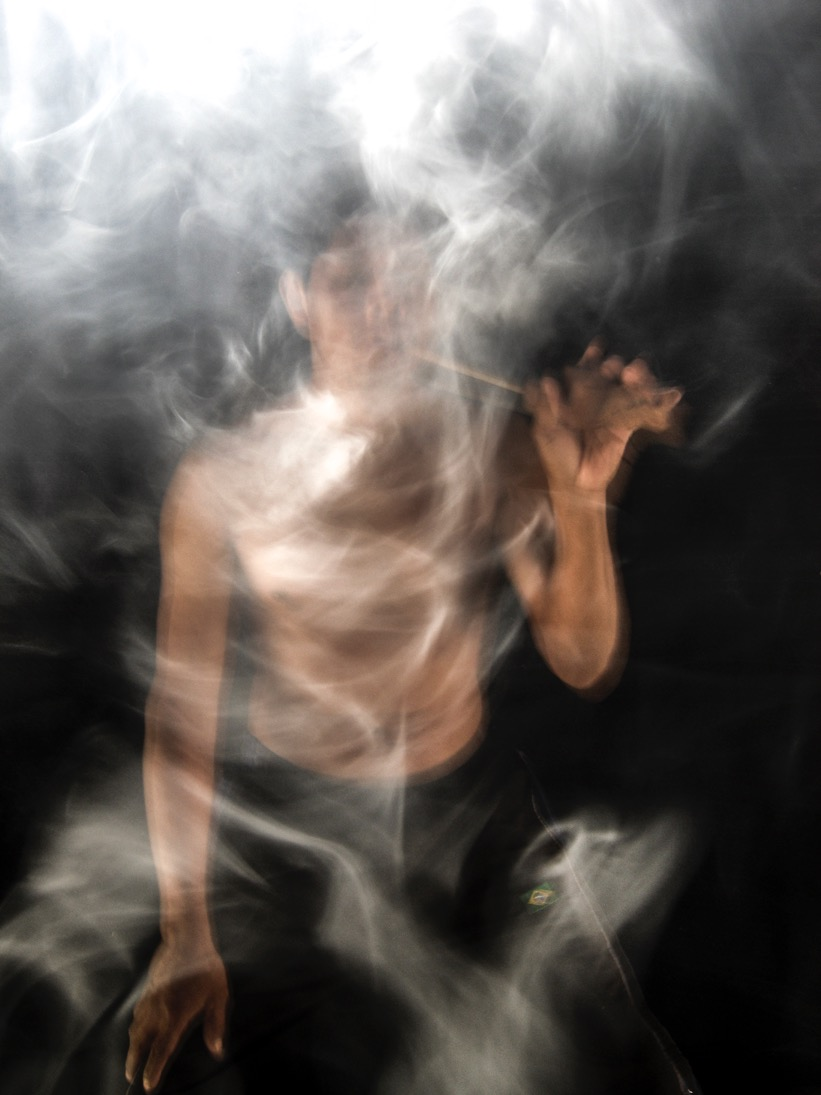
\includegraphics[width=4.572in,height=6.0984in]{livroredesguaranifinal-img3.jpg}
 

Rapaz mbya envolto na fuma\c{c}a do pet\~{y}gua (cachimbo). Foto:
Renilson Mirim Macena, 2012.

Sonhos e conhecimentos na vida guarani: uma experi\^encia de pesquisa na
universidade

Karai Mirim (Algemiro da Silva)\footnote{* Professor na aldeia Brakui,
Angra dos Reis/RJ.} 

Eu sou Karai Mirim\footnote{ Este texto resulta da transcri\c{c}\~ao e
edi\c{c}\~ao de duas falas de Karai Mirim durante o simp\'osio
{\textquotedblleft}CEstA nas Redes Guarani{\textquotedblright}, em 16 e
17/10/2013, acrescido de pequenos trechos de seu Trabalho de
Conclus\~ao de Curso na Universidade Federal Rural do Rio de Janeiro
(Nota das Organizadoras).}. Infelizmente tamb\'em tenho nome
portugu\^es, Algemiro. Como nomeado pelos antrop\'ologos, sou Guarani
Mbya, e sou professor na aldeia Brakui, tamb\'em chamada Sapukai. Nunca
deixei a aldeia, mas continuo estudando. Como um professor que foi
formado na Sociologia, acho muito importante fazer sempre interc\^ambio
com os Guarani e com os jurua.

O pensamento guarani foi negado pelos jurua ao longo do tempo. A gente
achava que o conhecimento dentro da comunidade, nossa viv\^encia, n\~ao
significava nada para os jurua. Mas a partir do momento que fui
estudando, minha pesquisa modificou muito esse pensamento. Minha
pesquisa me ajudou a pensar e a repensar a nossa cultura. \'E
importante fazer interc\^ambio porque existem v\'arias aldeias, cada
uma com sua forma\c{c}\~ao, cada professor guarani tamb\'em tem sua
forma\c{c}\~ao diferente. Ent\~ao \'e importante trazer o interc\^ambio
entre os Guarani tamb\'em, pra reunir o nosso conhecimento. Sabemos que
os Guarani se espalharam pelo Brasil, pelo continente, e ent\~ao cada
conhecimento tem sua hist\'oria. Com esse encontro, nosso conhecimento
talvez possa ajudar a sociedade n\~ao ind\'igena e a gente a viver
melhor.

Isso que eu escrevi, n\~ao escrevi ontem, n\~ao escrevi hoje, n\~ao.
Venho escrevendo h\'a anos. Na verdade, \'e uma pesquisa, como voc\^es
chamam. Eu fiz o curso de Licenciatura em Educa\c{c}\~ao do Campo na
Universidade Federal Rural do Rio de Janeiro, e aprendi que para os
jurua \'e importante escrever. Eu n\~ao pensei que era assim, para mim
a universidade era para participar e receber papel para eu dar aula na
comunidade. Mas cheguei l\'a e era diferente, tem que participar, tem
que fazer prova, tem que escrever... Era muito dif\'icil porque o
Guarani \'e mais de falar do que de escrever. Como botar o pensamento
guarani no papel? Na linguagem guarani tem a l\'ingua que \'e usada
diariamente e a linguagem que \'e usada dentro da opy, que \'e muito
dif\'icil para traduzir.

Vivo na aldeia Brakui, hoje chamada tamb\'em Sapukai, em Angra dos Reis,
no Rio de Janeiro. Nunca sa\'i da aldeia, desde crian\c{c}a, s\'o sa\'i
para estudar. A universidade manda fazer monografia, ent\~ao eu tive
que me esfor\c{c}ar muito para botar no papel meu pensamento e o
pensamento da comunidade. Foi dif\'icil. Eu moro na aldeia, tenho
rela\c{c}\~oes muito boas com a comunidade, mas percebi que pra fazer
pesquisa e perguntar para as pessoas do modo que a Universidade faz,
tendo que gravar, foi diferente.

No nosso jeito de ser, n\~ao \'e qualquer hora que podemos chegar e
pesquisar. N\~ao \'e assim que funciona com os Guarani. Tudo tem seu
tempo, como fala Vera Mirim, meu pai. Com ele demorei dois meses
somente para falar sobre o assunto da pesquisa. Para iniciar a nossa
conversa, sempre perguntava o que ele tinha sonhado na noite passada.
Ent\~ao eu conversava sobre outros assuntos, mas n\~ao era mais a
pesquisa. Era uma conversa sobre rem\'edios, hist\'orias, piadas. Ele
\'e muito brincalh\~ao, nossas conversas eram animadas e r\'iamos
bastante. S\'o muito depois que gravei uma entrevista. 

Ap\'os a perda de pessoas importantes de sua vida, Vera Mirim
come\c{c}ou a sonhar, oexa ra{\textquoteright}u. V\'arios Guarani j\'a
me contaram que os sonhos se intensificaram a partir de acontecimentos
tr\'agicos, tristes. Com Vera Mirim aconteceu o mesmo. Para voc\^e ser
um bom sonhador, \'e preciso viver de acordo com
teko~ete{\textquoteright}i: rezar bastante, participar de todas as
cerim\^onias, tem que ir \`a opy, se dedicar o m\'aximo poss\'ivel.

Eu escrevi sobre aldeia e sobre o sonho, como que os Guarani acham o
lugar para morar ou fazer tekoa a partir do sonho. Um colega meu que
era mais velho, infelizmente j\'a falecido, quando a gente morava l\'a
em Paranagu\'a (PR), ele me contou assim: {\textquotedblleft}Ah, ontem
eu fui l\'a pro Brakui{\textquotedblright}. Eu dei risada, todo mundo
deu risada. {\textquotedblleft}Como assim foi
l\'a?{\textquotedblright}. Ele falou: {\textquotedblleft}Fui l\'a,
andei por l\'a, tem cachoeira, tem \'agua, s\'o que n\~ao tem
peixe{\textquotedblright}, e no final ele contou que tinha sonhado
isso. Lembrando dessa hist\'oria, perguntei para o meu pai o que ele
tinha sonhado para chegar na aldeia de Brakui. A\'i ele falou que
quando tinha 13 anos ele j\'a sonhava com o lugar. Mas no sonho n\~ao
se v\^e exatamente igual. Ele sonhou, mas n\~ao sabia exatamente onde
era. Depois do sonho, passou um tempo, muito tempo depois, era no final
de 1989, e ele foi l\'a pra Brakui e viu tudo aquilo que ele sonhou.
Ent\~ao tudo tem essa rela\c{c}\~ao com o sonho.

Tem dois tipos de sonho: o da revela\c{c}\~ao e o que \'e exatamente o
sonho mesmo, oexa ra{\textquoteright}u. Pra gente oexa \'e ver, oexa
ra{\textquoteright}u \'e ver mas n\~ao ver, ver de olhos fechados. Oexa
ra{\textquoteright}u o lugar, e para conseguir escolher o lugar, tem
que ter mel que os deuses deixaram pra n\'os. Quando tem isso, j\'a
d\'a pra morar. E a\'i \'agua, montanhas, animais espec\'ificos tem que
ter pra gente poder morar. Ent\~ao escrevi sobre isso que meu pai
falou. Para fazer aldeia tem que ter um lugar considerado
ka{\textquoteright}aguy mir$\iota $[342?]. Mir$\iota $[342?] pode ser
entendido por {\textquotedblleft}pequeno{\textquotedblright}, mas tem
outra dimens\~ao, que \'e
{\textquotedblleft}sagrado{\textquotedblright}. L\'a na Universidade me
pediram para eu explicar o que \'e um local de ka{\textquoteright}aguy
mir$\iota $[342?]. Eu falei pra eles que ka{\textquoteright}aguy
mir$\iota $[342?] \'e o guarani que considera sagrado, n\~ao d\'a pra
descrever, pra mostrar a partir de certas coisas. Pra quem n\~ao
conhece n\~ao \'e nada, \'e s\'o um lugar.

Os sabedores na aldeia

Para estruturar a aldeia, tem que ter um s\'abio que d\'a nome para as
crian\c{c}as, para os Guarani, e tem que ter parteira. Porque n\~ao
tendo parteira n\~ao vai nascer crian\c{c}a. E nascendo crian\c{c}a,
depois de um ano, tem que receber o nome guarani. E o que falta mais?
Tem que ter conhecedor de rem\'edio. O pr\'oprio Vera Mirim (ou Jo\~ao
da Silva), meu pai, falou sobre isso, que tendo essas tr\^es pessoas,
tr\^es s\'abios, se consegue estruturar a aldeia: o que d\'a nome, a
parteira e o que faz rem\'edio.

\'E muito importante o papel da parteira na aldeia porque a hora do
parto \'e sagrada, \'e uma cerim\^onia, pra n\'os n\~ao \'e um parto
normal. O pai da crian\c{c}a deve estar presente e preparar uma estira
de taquara para cortar o cord\~ao umbilical. Tamb\'em deve enterrar a
placenta da crian\c{c}a dentro da casa.

Tem cinco parteiras l\'a na aldeia, e eu escolhi uma pra entrevistar. Eu
sei algumas coisas que meu pai me ensinou e a partir da\'i eu fiz as
perguntas. Elas falam que \'e muito dif\'icil agora devido ao jurua, os
brancos. Quando a crian\c{c}a nasce dentro do hospital n\~ao tem mais
cerim\^onia, ent\~ao \'e muito triste. Quando fiz entrevista, as
mulheres falaram que deveria ter di\'alogo do doutor com a parteira. 

Eu falo tamb\'em na pesquisa do ipopor\~a, que traduzindo literalmente
\'e {\textquotedblleft}m\~ao bonita{\textquotedblright}, porque ele tem
bastante conhecimento sobre ervas medicinais. Eu tenho esse
conhecimento e na aldeia v\'arios t\^em, mas eu n\~ao vou dizer que sou
ipopor\~a. Tamb\'em paj\'e n\~ao fala que \'e paj\'e. N\'os, vamos
dizer, {\textquotedblleft}usu\'arios{\textquotedblright}, que dizemos
que {\textquotedblleft}ele \'e paj\'e{\textquotedblright}.

O Jos\'e, conhecido por todos os Guarani como Karaja{\textquoteright}i,
ele sabe rem\'edio para curar doen\c{c}a, para arranjar namorado,
namorada, muitas coisas. Eu perguntei pra ele se podia resgatar a
hist\'oria e ele disse que podia, mas n\~ao permitiu tirar foto das
plantas. Ent\~ao eu disse {\textquotedblleft}tudo bem, n\~ao \'e pra
tirar mesmo, mas s\'o pra dizer que tem
conhecimento{\textquotedblright}. A\'i ele concordou em falar e
comentou tamb\'em um pouco do sonho. Desde o primeiro momento da
cria\c{c}\~ao do mundo os Guarani viviam no sonho. Mas \'e muito
preocupante que hoje em dia estamos sonhando outras coisas. Eu espero
que os Guarani sempre sonhem. Guarani sonha geralmente com animaizinhos
quando v\~ao ter filho. Primeiro sonha e depois confirma. Se for filho
homem sonha com animaizinhos maiores, geralmente com caititu. E quando
tiver filha sonha com ave. Esse sonho com os animaizinhos s\~ao
nhe{\textquoteright}\~{e}. Vera Mirim fala ~assim:
~{\textquotedblleft}Nhe{\textquoteright}\~{e} 
por\~a{\textquotedblright}, ~porque ~n\~ao ~\'e ~qualquer ~esp\'irito.
At\'e hoje, quando sonha com peixe, o sonho \'e realizado na
comunidade. Quando sonha com mel \'e gripe. Fogo \'e gripe mais grave.
Cobra \'e sinal que algu\'em est\'a com raiva de voc\^e. Eu escrevi
sobre isso na Universidade.

Quando souberam que fui formado na Universidade, Sociologia, todo mundo
perguntava e me abra\c{c}ava. Com isso, todos ficaram muito animados em
estudar. Mas a minha preocupa\c{c}\~ao \'e que os Guarani estudem e
voltem pra aldeia. Tem que sonhar da vida guarani, minha
preocupa\c{c}\~ao \'e isso. Estudar pode estudar, mas viver sempre em
Guarani, sonhar em Guarani.

Para fazer a pesquisa me senti diferente porque no dia-a-dia da minha
vida eu converso muito, brinco muito, conto piadas, conto as
hist\'orias dos antigos, conto hist\'oria de namoro, v\'arias
hist\'orias. Mas escrever sobre os sonhos, que foi meu tema de
pesquisa, foi dif\'icil. Mudou meu jeito de sonhar. Depois de estudar
quatro anos na Universidade, eu sonhava com carro, sonhava que estava
na sala de aula, fazendo prova... Quando sonhei com carro, pensei que
ia ganhar alguma coisa, mas nada. Da\'i eu pensei que todo mundo na
comunidade estava sonhando alguma coisa que n\~ao era guarani, e na
verdade era s\'o eu que n\~ao estava sonhando com as aldeias. S\'o meu
sonho que foi mudando.

Apesar da tecnologia, da televis\~ao, pelo menos na minha aldeia a casa
de reza est\'a l\'a, n\~ao fica abandonada. Ela fica no centro da
aldeia e \'e sempre frequentada, tem crian\c{c}ada no p\'atio, tem um
grupo de jovens. Os Guarani precisam de um karai pra dirigir a opy, a
casa de rezas, mas meu pai n\~ao frequenta muito desde que minha m\~ae
foi embora pro c\'eu e ele ficou sozinho. Ent\~ao os jovens entram
sozinhos, dan\c{c}am, rezam. Mas eu agrade\c{c}o meu pai, ele brinca
muito, ele tem cem anos de idade e diz que quer namorar ainda, isso \'e
muito legal\footnote{  Vera Mirim faleceu em 2016, posteriormente \`a
reda\c{c}\~ao deste texto.}.

Na minha pesquisa tamb\'em escrevi que desde o primeiro momento, na
cria\c{c}\~ao do mundo, ou na hist\'oria, a gente fala muito da
religi\~ao guarani. Mas dentro da religi\~ao guarani a gente n\~ao fala
s\'o da religi\~ao. Tem muitos momentos festivos, eu escutava muitas
hist\'orias antigas, de uma casa de reza bem grande.... Na casa de reza
n\~ao podia namorar, se entrava com a namorada e cada um sentava em um
canto. At\'e hoje a fam\'ilia fala para os jovens:
{\textquotedblleft}vai com o namorado, mas um senta aqui e outro l\'a,
aqui dentro da casa de reza n\~ao pode namorar{\textquotedblright}.

Nhandereko ete{\textquoteright}i \'e o jeito do guarani, mas tamb\'em se
fala na opy do nhandereko mar\~a e{\textquoteright}\~{y}, da vida dos
imortais. S\'o que n\~ao \'e qualquer pessoa que vai seguir nhandereko
mar\~a e{\textquoteright}\~{y} , \'e muito dif\'icil, \'e complicado. E
a\'i eu me lembro do filme que eu assisti,
{\textquotedblleft}Bicicletas de Nhanderu{\textquotedblright}. N\'os
Guarani somos guiados como uma bicicleta, mas n\~ao \'e qualquer um que
\'e bicicleta. A vida n\~ao \'e s\'o na casa de reza. Tem tempo de
namoro, tempo de casamento, tem tempo de alegria. \'E isso o que
acontece at\'e hoje.

As pessoas se fazem em redes, por saberes que s\~ao enredados e pelo
investimento em caminhos de percep\c{c}\~ao. A capacidade de
concentra\c{c}\~ao que muitos mencionaram \'e um modo amer\'indio de
formular a capacidade de buscar conhecimento e de n\~ao se perder em
outros caminhos. Importante ter sido colocada a quest\~ao de que os
mais velhos sabem mais. Eles t\^em condi\c{c}\~oes de
concentra\c{c}\~ao muito grandes e, eu imagino assim, est\~ao
transbordando de capacidade de passar conhecimentos. Isso mostra que o
conhecimento n\~ao \'e uma coisa a se enfiar na cabe\c{c}a, e sim uma
disposi\c{c}\~ao. Como mudar a escola para que isso possa ser aceito?
Como mudar a escola para se abrir para outras pr\'aticas de
conhecimento? Isso \'e uma quest\~ao absolutamente dif\'icil. --
Dominique Tilkin Gallois

Os xondaro e a circula\c{c}\~ao de saberes no mundo de hoje

Jera Poty Mir$\iota $[342?] (Giselda Pires de Lima)\footnote{*
Professora na escola da aldeia Tenonde Por\~a, S\~ao Paulo /SP.}  

Come\c{c}o dizendo que, mesmo sendo Guarani, mesmo tendo nascido numa
aldeia Guarani-Mbya, mesmo fazendo parte desse povo que tem
conhecimentos t\~ao belos, t\~ao fortes, ainda diria que eu sei pouco.
Todos os dias, o tempo inteiro eu aprendo muito com os xeram\~oi, com
as xejaryi, que s\~ao as pessoas mais velhas, mesmo que n\~ao sejam
l\'ideres espirituais. De fato, aqueles que t\^em mais idade sempre
sabem mais e eu fico muito feliz de estar constantemente aprendendo na
aldeia. A\'i eu passo um pouquinho desses conhecimentos para os amigos
que n\~ao s\~ao Guarani.

Os mais velhos sabem bastante, e eles mesmos trocam tamb\'em seus
saberes, j\'a que tem muitos pontos ou situa\c{c}\~oes dentro de um
saber que s\~ao diferentes. Mas aqueles que aprendem todos os dias
s\~ao as crian\c{c}as e os jovens. Posso falar s\'o pelas aldeias que
eu conhe\c{c}o mais, como a aldeia do Silveira, no litoral, onde eu vou
bastante e gosto muito. Tamb\'em pela aldeia de Krukutu, pela aldeia do
Jaragu\'a, que tamb\'em s\~ao da capital de S\~ao Paulo, como a minha
aldeia.

Eu nasci e estou h\'a 31 anos na aldeia Tenonde Por\~a. Ali muita coisa
mudou nos \'ultimos quinze ou vinte anos. Quando eu era crian\c{c}a
n\~ao tinha luz na aldeia, n\~ao tinha TV, s\'o alguns tinham radinho
de pilha, mas para comprar pilha tinham que estar com os jurua, e a
maioria n\~ao topava muito. A rela\c{c}\~ao com os jurua era muito
distante. Nessa \'epoca, era muito mais r\'apido aprender as coisas da
aldeia, o que a gente tinha que fazer como crian\c{c}as, ou como
jovens, ou como pessoas passando pelo ritual de passagem pra se tornar
adultos. A gente tinha uma aten\c{c}\~ao muito maior para os nossos
velhos, para as nossas m\~aes, para os nossos pais, porque n\~ao tinha
tantas outras influ\^encias.

Eu, quando ainda n\~ao era mocinha, esperava que isso acontecesse comigo
porque teria toda a fam\'ilia voltada pra mim: a minha irm\~a mais
velha, minha tia, minha m\~ae, minha av\'o. Todas elas se voltariam pra
mim pra me ensinar melhor como cozinhar, lavar roupa, costurar, cuidar
de outras crian\c{c}as... Tamb\'em era um momento de aprender muitas
outras coisas. Nessa fase de dez, doze, treze anos, catorze anos, a
gente est\'a num momento de muita curiosidade. A ideia de saber que
muitas pessoas velhinhas iam ensinar muitas outras coisas era muito
esperado.

No mundo de hoje, na Tenonde-Por\~a e em algumas outras aldeias que eu
conhe\c{c}o, eu acho que esse conhecimento ainda est\'a muito forte,
mesmo quando est\'a meio que dormindo... De fato, hoje tem uma grande
influ\^encia do mundo do jurua por conta da energia el\'etrica e da
tecnologia. No mundo guarani tamb\'em isso est\'a ficando muito mais
forte. Todo mundo tem acesso \`a internet, acesso \`a escola, e cada
vez mais os jovens e as crian\c{c}as ficam muito presos nessa forma de
saber. A gente pode pensar: {\textquotedblleft}as crian\c{c}as e jovens
est\~ao muito presos na internet, no celular, na escola, mas tem os
adultos que sabem da cultura, que dominam a l\'ingua e os princ\'ipios
guarani, ent\~ao esses n\~ao v\~ao deixar a peteca
cair{\textquotedblright}. S\'o que \`as vezes pais e m\~aes, muitos
xeram\~oi infelizmente tamb\'em ficam assistindo TV em casa. Por que o
filho, se for assalariado, comprou uma TV de plasma muito bonita, que
tem uma imagem muito de outro mundo, e a\'i gostam tamb\'em de assistir
filmes de a\c{c}\~ao, como o filme do
{\textquotedblleft}Avatar{\textquotedblright}, que tem efeitos
especiais. Os mais velhos tamb\'em ficam muito encantados com isso e
\`as vezes deixam de fazer a roda de hist\'oria com esses que j\'a
vivem num mundo muito cheio de influ\^encias tecnol\'ogicas. 

Vou tentar contar alguns pontos mais fortes dessa experi\^encia de ser
Jera, de ser moradora da aldeia Tenonde-Por\~a, de ter nascido nessa
cultura, de trabalhar na \'area da educa\c{c}\~ao, dentro da pouca
experi\^encia que tenho de trabalhar como educadora, mas de sempre ter
pensado como fazer com que a escola n\~ao interferisse de maneira muito
agressiva na educa\c{c}\~ao tradicional. Todas as vezes que me envolvi
em projetos pra fortalecer nossa cultura, que veio se prejudicando por
conta da pouca terra e de n\~ao ter mata em muitas aldeias, se
envolveram comigo muitos jovens e crian\c{c}as, e alguns pais. Talvez
os adultos se envolvam menos porque eles j\'a sabem bastante, mesmo que
j\'a n\~ao fa\c{c}am atividades de ca\c{c}a, de pesca, j\'a que n\~ao
tem como fazer na \'area. Eles n\~ao fazem porque n\~ao tem como fazer,
mas sabem.

O fato \'e que quando voc\^e chama as pessoas pra uma conversa voltada
para esse tema de fortalecer a cultura guarani, a maioria \'e sempre de
crian\c{c}as e jovens. \`As vezes os mais velhos falam para os novos:
{\textquotedblleft}voc\^es n\~ao querem mais comer fub\'a, voc\^es
n\~ao querem mais comer milho, voc\^es n\~ao querem mais comer mbyta,
rora, que s\~ao as comidas tradicionais{\textquotedblright}. O problema
\'e que quando eles t\^em seis, sete aninhos, n\~ao s\~ao eles que
v\~ao para o mercado de jurua, s\~ao os pais. Ent\~ao o que o filho
sabe comer hoje foi o pai e a m\~ae que ensinou. N\~ao adianta o menino
fazer quinze anos e quererem enfiar goela abaixo um mbyta (comida feita
de milho)...

O despertar dos xondaro

Mesmo quando o sentido de ser guarani, o esp\'irito, a alma de ser
guarani est\'a um pouco dormindo, quando \'e chamado ele acorda muito
r\'apido. A gente come\c{c}ou um projeto de fortalecimento do xondaro
na Tenonde-Por\~a em 2010, quando ele estava muito, muito adormecido.
Xondaro, que s\~ao os guardi\~oes, era uma coisa que sempre me
emocionava bastante quando eu era crian\c{c}a. Quando os xondaro
dan\c{c}avam, eu ficava sentadinha e sentindo o ch\~ao embaixo de mim
tremendo. Era uma vibra\c{c}\~ao muito forte, uma coisa linda,
magn\'ifica. Os homens dan\c{c}am com muita seriedade porque faz parte
do mundo espiritual guarani, que tem uma concep\c{c}\~ao muito ampla,
grandiosa.

Depois eu fui crescendo e a dan\c{c}a do xondaro foi se enfraquecendo na
aldeia. Eu falava para os meus parentes da Tenonde Por\~a que a gente
precisava fortalecer, trazer de volta o xondaro que estava dormindo. O
xondaro est\'a muito voltado para o contexto espiritual, de ter seu
valor como Guarani, mas tamb\'em \'e uma pr\'atica de dan\c{c}a que
mexe muito com a for\c{c}a f\'isica. Algumas lutas, por exemplo o
karat\^e, tem movimentos em que voc\^e tem que ficar com os m\'usculos
muito tensos pra voc\^e atacar bem, pra voc\^e derrubar o seu inimigo.
J\'a no xondaro \'e ensinado a ter a leveza no corpo. Eu posso jogar
algu\'em a quil\^ometros de dist\^ancia com a leveza do meu corpo,
mesmo que a pessoa esteja enrijecida, na defensiva.

Ser xondaro ou xondaria n\~ao significa s\'o circular, dan\c{c}ar, pular
e rodar... significa voc\^e incorporar o esp\'irito guarani e, a partir
da\'i, saber o que voc\^e pode fazer e o que n\~ao pode, se voc\^e \'e
xondaro ou xondaria de quem, de quem voc\^e tem que cuidar dentro da
sua aldeia e como voc\^e tem que cuidar. Tamb\'em saber como v\~ao ser
seus passos no futuro, dentro da comunidade que voc\^e vive, pra que
voc\^e seja o xondaro que voc\^e tenta ser quando voc\^e entra no
c\'irculo da dan\c{c}a. A beleza do xondaro, toda sua concep\c{c}\~ao,
voc\^e s\'o entende se voc\^e for na aldeia e ver algumas dan\c{c}as,
ou se voc\^e dan\c{c}ar.

Quando come\c{c}amos o projeto, lembro que nas primeiras tentativas de
dan\c{c}a, de levar as crian\c{c}as e os jovens pra casa de reza,
estava todo mundo meio endurecido. Mas com o come\c{c}o do projeto foi
muito r\'apida a desenvoltura do corpo, o retorno do esp\'irito dos
xondaro, mesmo para aqueles que sabem pouco da concep\c{c}\~ao profunda
do xondaro, como os pequeninhos de tr\^es, quatro anos, que eram todos
meio durinhos e agora fazem coisas lindas, muito fortes. 

Um dos mestres xondaro, Pedro Vicente, falou muito para os jovens como
\'e que as pessoas t\^em que ser pra aprenderem de verdade o xondaro.
Com as palavras de Pedro Vicente, muitos jovens mudaram o comportamento
e come\c{c}aram a pensar diferente sobre a situa\c{c}\~ao de estarem
muito presos a um mundo que n\~ao faz parte da sua cultura. A Tenonde
Por\~a tem 26 hectares, n\~ao tem natureza, n\~ao tem como ter contato
com animais, com \'agua, com pesca, com ca\c{c}a... ent\~ao pesa mais a
influ\^encia tecnol\'ogica do jurua, da energia el\'etrica. Para alguns
homens guarani, quando n\~ao tem o que pescar, n\~ao tem o que
ca\c{c}ar e n\~ao tem como entrar na mata e cortar \'arvores pra fazer
suas casas, tamb\'em \`as vezes n\~ao tem porque ir pra casa de reza,
pra fortalecer aquilo que n\~ao est\'a muito saud\'avel.

Por isso, no projeto a gente contou com lideran\c{c}as e amigos de
outras aldeias que tem seus espa\c{c}os maiores, que tem mais natureza,
como na aldeia do Silveira. Ent\~ao aconteceram coisas lindas, a gente
se fortaleceu, e os jovens da Tenonde-Por\~a se fortalecerem enquanto
xondaro. Depois a gente tamb\'em teve a oportunidade de levar os
xondaro da Tenonde Por\~a que j\'a estavam animados, que j\'a estavam
acordados, pra outras aldeias em que esse conhecimento estava tamb\'em
um pouco dormindo. Mesmo estando em aldeias diferentes, a gente \'e um
povo s\'o e se entende bastante nesse sentido.

Cada mestre xondaro tem suas particularidades, sua concentra\c{c}\~ao,
sua leveza corporal. Quando entram na roda, cada xondaro e xondaria tem
que ir com seriedade porque est\~ao dan\c{c}ando tamb\'em pros Nhanderu
kuery, para os nossos deuses, pra gente se fortalecer. Ent\~ao voc\^e
nunca pode entrar rindo. O Karai Xondaro, l\'a na aldeia do Silveira,
parava na frente dos xondaro que n\~ao estavam concentrados e ficava
olhando, sem falar nada, at\'e que eles percebecem e parassem de rir ou
de falar. Isso acontecia de uma maneira muito bonita. Esse Karai
Xondaro tem uma concentra\c{c}\~ao total, que n\~ao \'e enrijecida. Ele
tinha uma yvyra raimbe, que \'e uma madeira comprida, e fazia muito
forte a dan\c{c}a do xondaro. Ele passava a madeira muito r\'apido para
os meninos se esquivarem e eu pensava que eles iam ser atingidos. Em
muitos momentos eu senti meu cora\c{c}\~ao ficar bem duro, porque
parecia que ele ia atingir esses xondaro que estavam dan\c{c}ando com
ele e que estavam ainda aprendendo, pois era o come\c{c}o do projeto.
Eu percebia o medo no rosto do meu sobrinho. Eu queria salvar todo
mundo que estava l\'a, mas pensei: {\textquotedblleft}n\~ao, esse
xondaro ruvixa sabe o que est\'a fazendo, n\~ao vai atingir, vai ficar
tudo bem{\textquotedblright}. Ent\~ao aconteceu uma coisa linda, porque
todos esses xondaro que estavam dan\c{c}ando com eles incorporaram,
definitivamente, o esp\'irito dos xondaro guarani, passaram a se
concentrar mesmo.

A gente teve h\'a pouco tempo movimentos muito fortes que vieram a
partir desses xondaro que foram acordados. Mesmo quando os xondaro
n\~ao est\~ao dan\c{c}ando, n\~ao est\~ao ativos na aldeia, os Guarani
em todas as situa\c{c}\~oes de precis\~ao um do outro se unem, a gente
senta junto, conversa junto, a gente vai junto. Nos \'ultimos dois anos
eu senti muito forte o movimento dos xondaro em v\'arios cantos dos
territ\'orios guarani ficar mais forte. Cada vez fica mais forte os
xondaro se sentirem xondaro na situa\c{c}\~ao de cuidarem um do outro
e, a partir disso, quererem fazer as coisas sem descanso. Est\'a
acontecendo um movimento espiritual tamb\'em de fazer as coisas
acontecerem e de se cuidar na aldeia. Quando tem problema, por exemplo,
de bebida alco\'olica na aldeia, os rapazes dizem:
{\textquotedblleft}voc\^e tem que beber menos, voc\^e \'e xondaro!
Voc\^e n\~ao pode fazer isso. Assim n\~ao d\'a!{\textquotedblright}.
Eles t\^em essa cobran\c{c}a um com o outro, e tamb\'em de quererem
fazer as coisas como eu disse antes, sem dormir, por muito mais tempo,
pra acordar.

Isso tudo est\'a ligado aos movimentos ind\'igenas quanto \`as
quest\~oes das terras, da demarca\c{c}\~ao das terras. Teve o primeiro
movimento que aconteceu na rodovia dos Bandeirantes, que a gente fechou
pra protestar contra a demora nas demarca\c{c}\~oes, perto da aldeia de
Jaragu\'a. Depois a passeata na Avenida Paulista, que era pelas
demarca\c{c}\~oes e contra a PEC 215. Na Tenonde-Por\~a e na Krukutu, a
gente tamb\'em est\'a fazendo um movimento de retomada de nossas terras
de ocupa\c{c}\~ao tradicional. H\'a seis dias a gente retomou a aldeia
Kalipety, que era habitada por nosso povo na d\'ecada de 70. Eu queria
estar fazendo essa conversa que eu estou fazendo com voc\^es l\'a. Se
eu pudesse transportar todo mundo pra l\'a seria bom, s\'o pra voc\^es
sentirem isso como eu estou sentindo.

Nesses seis dias, h\'a momentos em que a gente foi ficando cansado,
fisicamente. A gente ia desanimando, mas a\'i o xeram\~oi punha a m\~ao
na nossa cabe\c{c}a e falava {\textquotedblleft}nembaraete
katu{\textquotedblright}, que \'e uma forma de nos alimentar
espiritualmente. A\'i ficava todo mundo muito animado de novo!
{\textquotedblleft}Bora fazer casa!{\textquotedblright},
{\textquotedblleft}Bora l\'a, ent\~ao!{\textquotedblright}. 

Esse \'e um come\c{c}o, a gente ainda est\'a ganhando experi\^encia. Mas
a retomada de terras tradicionais \'e muito marcante para o povo
guarani. Se algumas pr\'aticas da cultura guarani estavam dormindo, mas
conseguiram acordar mesmo em \'areas que n\~ao tem natureza, imagina o
que pode acontecer numa \'area ampla e que tenha \'agua, que tenha
cachoeira, que tenha o que ca\c{c}ar? Ontem mesmo eu estava falando
para os meninos: {\textquotedblleft}imagina aqui quando voc\^es matarem
uma ca\c{c}a de grande porte e a gente poder distribuir pra todo
mundo?{\textquotedblright}. N\~ao vou repetir as palavras que eles
falaram, mas ficaram bem empolgados!

A escola e os saberes

A maioria de projetos que eu escrevo para fazer na aldeia \'e de
{\textquotedblleft}transmiss\~ao de saberes{\textquotedblright}, mas
estou gostando mais da ideia de
{\textquotedblleft}circula\c{c}\~ao{\textquotedblright}. Nessa
circula\c{c}\~ao de a\c{c}\~oes voltadas para o aprendizado informal,
diferenciado, tradicional, o que me preocupa bastante \'e esse modelo
da educa\c{c}\~ao que a gente tem hoje dentro das aldeias Guarani-Mbya.
Esse modelo nasceu da Constitui\c{c}\~ao, que assegura o direito da
crian\c{c}a ind\'igena a ter uma educa\c{c}\~ao diferenciada, tanto
dentro do mundo da sociedade envolvente como no mundo tradicional. Mas
para os Guarani-Mbya a educa\c{c}\~ao diferenciada \'e muito recente.

O povo Guarani foi um dos primeiros povos a ter contato com os jurua. E
ainda assim, em aldeias como a Tenonde Por\~a, o Silveira, Krukutu,
aldeias muito pr\'oximas da cidade, muito pr\'oximo de toda a
influ\^encia do jurua, ainda t\^em pessoas que n\~ao sabem falar o
portugu\^es, que se mant\^em muito no mundo Guarani. Diante disso,
quando a escola entrou na aldeia, os que est\~ao muito no mundo dos
Guarani n\~ao estavam dispostos a conversar sobre qual tipo de
educa\c{c}\~ao que a gente vai fazer na escola. O que se tinha era uma
coisa muito superficial, de que a gente precisa aprender a falar a
l\'ingua do jurua pra saber lidar melhor com as coisas do jurua que
chegam na aldeia. 

No in\'icio, quando eu tinha doze ou treze anos, eu lembro bem que a
ideia de aprender a l\'ingua ou os conhecimentos jurua era pra lutar
pelos direitos, era para coisas espec\'ificas... Como as pessoas que
estavam indo pra Bras\'ilia e que n\~ao sabiam falar direito o
portugu\^es, e que tinham que aprender a escrever e a ler, enfim, ter
capacidade de fazer decodifica\c{c}\~oes de documentos complicados, por
exemplo, a fim de n\~ao ser enrolado. S\'o que a\'i foi indo, foi indo,
foi indo e o que a gente tem hoje \'e isso, al\'em de voc\^e ter que
aprender pra se defender da cultura do jurua, se politizar e conhecer
seus direitos, a escola est\'a trazendo uma ideia de
padroniza\c{c}\~ao, de que voc\^e tem que ir pra escola pra ter um
trabalho, pra ter um dinheiro e a\'i voc\^e pode tamb\'em ser igual
\`aquele que tem um carro...

A gente n\~ao soube lidar com esse modelo de escola quando ele entrou na
aldeia. Ainda hoje n\~ao sabemos direito, e h\'a muitos conflitos com
outros professores, com a comunidade, com os representantes das
pol\'iticas. Eu tinha pensado como seria bom ter uma semana de escola e
outra sem escola, e fiz essa proposta na \'ultima Confer\^encia
Estadual de Educa\c{c}\~ao Ind\'igena. Mas ningu\'em concordou comigo!

A escola descaracteriza muito o cotidiano das comunidades guarani.
Quando a crian\c{c}a guarani tem um tempo r\'igido para ir para escola
e tem que cumprir um hor\'ario, aos poucos vai perdendo a delicadeza em
respeitar o seu momento. Por exemplo, as meninas quando est\~ao
menstruadas n\~ao devem ir para a escola, mas isso quase nunca \'e
respeitado.

Antes eu ficava meio depressiva, mas hoje fico feliz porque \`as vezes o
jurua fala eu n\~ao entendo tudo. \`As vezes quando o Guarani fala eu
tamb\'em n\~ao entendo tudo, e a\'i eu penso: {\textquotedblleft}nossa
como eu tenho que aprender ainda!{\textquotedblright}. E isso \'e bom.
\`As vezes um xeram\~oi est\'a falando na casa de reza e eu me sinto
analfabeta na minha pr\'opria l\'ingua, n\~ao entendo quase nada do que
est\'a sendo dito. O xeram\~oi Pedro Vicente tinha dito pra mim que,
pra gente ser uma pessoa com dom, pra saber contar hist\'orias,
tamb\'em tinha que ter arakuaa. Ele n\~ao falou arandu, que \'e uma
palavra usada para {\textquoteleft}conhecimento{\textquoteright},
{\textquoteleft}sabedoria{\textquoteright}. Ele disse que aprender
escrever \'e ter arandu, \'e ser inteligente. Mas o arakuaa est\'a mais
voltado para uma quest\~ao espiritual, que \'e uma linguagem mais
voltada e mais usada no mundo da opy. Assim, hoje existem v\'arios
meios de conhecimento... tem xeram\~oi, tem Google, tem os livros, os
antrop\'ologos, entre muitos outros...

A palavra xondaro, que quer dizer tanta coisa, para os Guarani Mbya \'e
como que uma met\'afora da rela\c{c}\~ao de uma pessoa que est\'a
conduzindo o processo e dos auxiliares que est\~ao dispostos a levar
esse processo adiante. Isso me leva \`a quest\~ao da rela\c{c}\~ao das
divindades concebidas como os irm\~aos mais velhos dos homens. O pai do
seu Algemiro me contou que quando o primeiro Nhanderu criou o irm\~ao,
ele criou uma c\'opia transformada de si mesmo. E da\'i eu fiquei
pensando no processo de educa\c{c}\~ao como o imitar, como a
crian\c{c}a est\'a sempre imitando os adultos e a partir disso est\~ao
aprendendo. S\'o que est\~ao imitando e transformando esse
conhecimento. Esses irm\~aos mais velhos s\~ao o modelo, mas n\~ao
necessariamente um modelo fixo. \'E preciso sempre estar
experimentando, porque imitar \'e sempre transformar. - Daniel Calazans
Pierri 

Processos de aprendizado pelos olhos das crian\c{c}as guarani mbya

Alice Haibara\footnote{* Mestre em antropologia pela USP e membro do
CEstA.}

O objetivo deste texto \'e refletir sobre como se d\~ao os processos de
aprendizado entre as crian\c{c}as guarani mbya, analisando
principalmente o contexto da aldeia Tenonde Por\~a, que fica localizada
na regi\~ao sul da cidade de S\~ao Paulo\footnote{ Este artigo \'e
baseado em uma pesquisa de inicia\c{c}\~ao cient\'ifica, realizada
durante o per\'iodo de gradua\c{c}\~ao entre os anos de 2010 e 2011,
pelo Departamento de Antropologia USP, com orienta\c{c}\~ao de
Dominique Tilkin Gallois. As an\'alises e os dados aqui apresentados
foram produzidos em colabora\c{c}\~ao com a professora Jera Guarani, a
quem agrade\c{c}o imensamente.}. A partir da observa\c{c}\~ao de
diferentes contextos, pretende-se evidenciar alguns aspectos dos
diversos modos de constru\c{c}\~ao e circula\c{c}\~ao de saberes entre
os Guarani, para ent\~ao refletir sobre como estes modos pr\'oprios de
conhecer se relacionam com as formas de aprendizado caracter\'isticas
da escola.

Os pressupostos da pesquisa se baseiam numa atual Antropologia da
Crian\c{c}a, em que as crian\c{c}as s\~ao vistas como participantes
ativas de seus processos de aprendizado e n\~ao como um mero
recept\'aculo de informa\c{c}\~oes (Cohn, 2000). Desta forma as
crian\c{c}as s\~ao compreendidas com base na constru\c{c}\~ao de um
universo que lhes \'e pr\'oprio, considerando que elas possuem
conhecimentos qualitativa e n\~ao quantitativamente diferenciados do
mundo adulto (idem, 2000). Quando buscamos entender as crian\c{c}as e
seu contexto social a partir do ponto de vista delas mesmas, \'e
poss\'ivel construir uma apreens\~ao que \'e diferenciada e relevante,
sendo poss\'ivel muitas vezes evidenciar aspectos sociais que n\~ao
s\~ao expl\'icitos (Toren, 1993). Neste sentido, buscamos ouvir e dar
visibilidade ao que as crian\c{c}as guarani pensam, como concebem o
mundo em que vivem, como compreendem a si mesmas, seus corpos, suas
express\~oes, seus aprendizados e experi\^encias. 

As kyringue guarani mbya

Entre os Guarani, as crian\c{c}as t\^em um lugar de grande
import\^ancia. De acordo com alguns interlocutores, a partir do momento
em que diminu\'irem ou acabarem as crian\c{c}as, Nhanderu
({\textquoteleft}Nosso Pai{\textquoteright}) acabar\'a com a vida na
Terra. Jera Guarani (2008: 39) afirma que:

O povo Guarani compreende que o esp\'irito da crian\c{c}a \'e enviado
por Nhanderu (...) sempre com uma miss\~ao: \`as vezes para fortalecer
o pai, a m\~ae, ou at\'e mesmo os av\'os, e em algumas situa\c{c}\~oes
para fortalecer o bem estar da uni\~ao entre o casal. Por isso a
crian\c{c}a era recebida com muito amor e carinho e, acima de tudo, com
muito respeito, pois para os Guarani o esp\'irito se liberta desta
viv\^encia humana para a morada sagrada de Nhanderu e volta como
crian\c{c}a, muitas vezes com o mesmo tipo f\'isico, ou alguma outra
caracter\'istica do que j\'a fora um adulto ou um velhinho, em vidas
passadas. A crian\c{c}a representa para o povo Guarani a vontade do
Criador, em dar continuidade \`a vida para o nosso planeta.

Existem diversas pr\'aticas e cuidados feitos na ocasi\~ao do nascimento
de uma crian\c{c}a, desde o momento da gesta\c{c}\~ao at\'e o per\'iodo
do p\'os-parto. Tais pr\'aticas visam \`a forma\c{c}\~ao da pessoa, de
maneira que os processos atravessados pelo esp\'irito se relacionam
diretamente \`as a\c{c}\~oes de fabrica\c{c}\~ao do corpo. Dentre
diferentes medidas podemos citar algumas, como quando a m\~ae faz um
pequeno colar com o cord\~ao umbilical do beb\^e e deixa pendurado em
seu pesco\c{c}o at\'e que ele seque, ou a pr\'atica do pai enterrar a
placenta em um buraco dentro da casa. Ambas atitudes visam fazer com
que a crian\c{c}a tenha um esp\'irito assentado e se torne uma pessoa
concentrada (Lima, 2008).

Entre as concep\c{c}\~oes e pr\'aticas guarani \'e not\'orio perceber
que o esp\'irito da crian\c{c}a est\'a intimamente relacionado ao pai e
as suas a\c{c}\~oes. De acordo com Jera Guarani, durante os primeiros
seis ou sete meses de vida da crian\c{c}a, o homem deve continuar seus
afazeres, mas seguindo um ritmo mais baixo, n\~ao realizando atividades
bruscas, como carpir ou cortar coisas. Por exemplo, se ele cortar uma
\'arvore, esta poder\'a cair sobre o esp\'irito da crian\c{c}a e a
mesma ficar\'a doente. Tamb\'em n\~ao se deve jogar futebol, pois como
o esp\'irito do filho passa o tempo todo com o pai, e se este ficar
correndo para l\'a e para c\'a, a crian\c{c}a vai se cansar muito, uma
vez que seu esp\'irito vai tentar fazer todas as atividades que o pai
est\'a fazendo. Quando isso ocorre os Guarani dizem que a crian\c{c}a
est\'a harua (cansada e sentindo inc\^omodos ou c\'olicas), e as
pessoas costumam afirmar: {\textquotedblleft}Seu filho est\'a harua,
voc\^e fica tendo comportamentos errados!{\textquotedblright}. Tamb\'em
a presen\c{c}a do pai pr\'oximo ao filho se faz muito importante, de
modo que o homem {\textquotedblleft}n\~ao deve se ausentar por muito
tempo, sair ou viajar nos primeiros meses de vida da
crian\c{c}a{\textquotedblright} (Melo, 2008: 85). Como a alma da
crian\c{c}a est\'a fortemente ligada ao pai depois do parto, ele deve
sempre marcar os caminhos que percorre, para que a alma do seu filho
n\~ao se perca (Clastres, 1978).

A import\^ancia em fazer com que a alma da crian\c{c}a permane\c{c}a
forte no corpo \'e algo presente nas concep\c{c}\~oes e nas pr\'aticas
guarani (assim como em diversos outros grupos amer\'indios), dessa
forma deve-se evitar que a crian\c{c}a chore ou fique triste, pois isso
pode fazer com que seu esp\'irito queira retornar para o lugar celeste
de onde veio. Assim, para alegrar e acalmar os beb\^es, \'e ensinado
\`as m\~aes que elas devem caminhar e cantar os mit\~a monguea
(can\c{c}\~oes de ninar). J\'a os mborai ete (cantos verdadeiros),
realizados durante as cerim\^onias na opy (casa de reza), n\~ao devem
ser cantados para os beb\^es muito pequenos porque s\~ao can\c{c}\~oes
ensinadas e enviadas aos yvyra{\textquoteright}ija (lideran\c{c}as
espirituais), de modo que o beb\^e poderia se recordar da morada
sagrada e assim querer retornar para l\'a antes de cumprir sua
miss\~ao.

De acordo com Testa (2008), entre os Guarani h\'a uma ideia
frequentemente afirmada de que {\textquotedblleft}a vida de cada um \'e
seu caminho de buscar e aprender{\textquotedblright}. A pesquisadora
associa o processo de aprendizado \`a no\c{c}\~ao de um caminho a
percorrer. Nesse sentido, \'e poss\'ivel dizer que desde a ocasi\~ao do
nascimento da crian\c{c}a j\'a s\~ao realizadas diversas a\c{c}\~oes
para que se tenha concentra\c{c}\~ao e direcionamento no caminho de
vida e aprendizado (relacionadas ao destino da placenta e cord\~ao
umbilical, por exemplo), e tamb\'em para facilitar o
{\textquotedblleft}caminhar junto{\textquotedblright}, quando o pai
{\textquotedblleft}marca os caminhos{\textquotedblright}, ou mesmo
quando evita realizar atividades em que o esp\'irito da crian\c{c}a
ter\'a dificuldade de acompanh\'a-lo. Desta forma, \'e poss\'ivel dizer
que as a\c{c}\~oes de {\textquotedblleft}acompanhar{\textquotedblright}
os pais e m\~aes imitando as suas pr\'aticas e comportamentos j\'a
s\~ao realizadas pela pessoa quando ela ainda est\'a na barriga da
m\~ae. O mesmo sentido \'e poss\'ivel dar \`as pr\'aticas que visam
manter o esp\'irito da crian\c{c}a forte no corpo, pois assim a pessoa
n\~ao ir\'a seguir o caminho de retorno \`a morada de Nhanderu antes do
tempo, podendo realizar seu caminho de aprendizado na Terra. 

As a\c{c}\~oes de fabrica\c{c}\~ao do corpo, relacionadas aos processos
do esp\'irito, mostram que entre os Guarani o conhecimento \'e
constru\'ido {\textquotedblleft}caminhando e aprendendo
junto{\textquotedblright}, o que pode ser entendido tamb\'em como um
tipo de rede de rela\c{c}\~oes entre os sujeitos envolvidos na
forma\c{c}\~ao da pessoa. Tal rede se constitui especialmente pelas
rela\c{c}\~oes entre os corpos e \'e por meio da corporalidade que a
pessoa guarani aprende a construir e direcionar seu caminho. Adentrando
no contexto da opy (casa de reza), \'e poss\'ivel verificar algumas
pr\'aticas de {\textquotedblleft}aprender junto{\textquotedblright}
realizadas no corpo e por meio do corpo.

Na opy

Na Aldeia Tenonde Por\~a, no in\'icio da noite, algumas pessoas se
re\'unem na opy.  As mulheres acendem o fogo e esquentam a \'agua para
tomar ka{\textquoteright}a (erva-mate). As pessoas sentam-se em volta
da fogueira em bancos e cadeiras conversando descontraidamente, alguns
cobertores s\~ao estendidos no ch\~ao, onde se acomodam mulheres com
suas crian\c{c}as. As crian\c{c}as pequenas mamam e brincam, dormindo
quando sentem vontade. Os petyngua (cachimbo) v\~ao sendo acesos, os
homens v\~ao se levantando e caminham num trajeto circular at\'e o
amba{\textquoteright}i (altar), seguem fumando e assoprando a
fuma\c{c}a em todo o redor. Algumas crian\c{c}as fazem o mesmo,
geralmente os meninos e tamb\'em algumas meninas, embora com menos
frequ\^encia. O som do viol\~ao come\c{c}a a soar e as pessoas se
levantam para cantar e dan\c{c}ar. 

O papel das crian\c{c}as na opy \'e muito importante, cantando,
dan\c{c}ando e participando ativamente. Durante algumas conversas, elas
demonstraram ter interessantes compreens\~oes em rela\c{c}\~ao \`as
pr\'aticas realizadas neste contexto, relacionando-as com os processos
de comunica\c{c}\~ao e intera\c{c}\~ao com diferentes aspectos da
cosmologia guarani. Assim, Kerexu, de dez anos, explicou o papel do
xeram\~oi (lideran\c{c}a espiritual masculina, traduzido como
{\textquotedblleft}meu av\^o{\textquotedblright}) e demonstrou
atrav\'es de gestos e sons como ele realiza as curas, fazendo uso das
m\~aos e da boca, por meio de sopro, suc\c{c}\~ao, cantos e do
petyngua. De acordo com a menina, o xeram\~oi arrasta a m\~ao nas
costas e na barriga da pessoa at\'e formar uma pedrinha que ele entrega
para o xondaro  ({\textquotedblleft}os guardi\~oes da opy e da
aldeia{\textquotedblright}, em sua defini\c{c}\~ao), que d\'a para a
xejaryi (lideran\c{c}a espiritual feminina, traduzido como
{\textquotedblleft}minha av\'o{\textquotedblright}) jogar no fogo. 

Kerexu afirma que esta pedrinha \'e de Anh\~a, traduzida pela menina
pelo termo {\textquotedblleft}satan\'as{\textquotedblright}, e que \'e
jogada no fogo para que {\textquotedblleft}Anh\~a pegue de novo a pedra
dele{\textquotedblright}. Ao falar sobre o processo em que as pessoas
ficam doentes por causa da pedrinha, ela descreve:

Quando as pessoas rezam muito e s\~ao de Nhanderu, diz que o Anh\~a fica
muito bravo, e a\'i quando a gente anda --- minha m\~ae que me contou
--- as pessoas que j\'a s\~ao mortas pegam uma pedra, que n\~ao \'e
venenosa, mas tem maldi\c{c}\~ao, e jogam. A\'i \'e doen\c{c}a de
Anh\~a quando a pessoa fica muito mal mesmo. Sabe quando o xeram\~oi
fica {\textquotedblleft}argh, argh{\textquotedblright}
[sonoriza\c{c}\~ao], \'e que tem uma pedrinha envenenada que eles tiram
da pessoa e jogam no fogo.

Kerexu afirma saber como o xeram\~oi realiza as curas porque ela mesma
j\'a passou pelo tratamento:

\'E porque ele j\'a tirou uma pedra de mim. Na verdade eu n\~ao estava
sonhando direito, eu dormia muito mal e sonhava muito com coisas ruins.

Ao ser perguntada sobre o motivo da doen\c{c}a ser retirada das costas,
a menina responde:

Por que a sombra vem daqui de tr\'as, a gente anda, fica feliz. O Anh\~a
joga a pedrinha s\'o em quem vai pra opy, quem reza mais. Os b\^ebados
ele deixa ficarem felizes sem doen\c{c}a. Mas da pinga eles ficam
doentes.

Kerexu afirma ainda que quando ficar velhinha quer muito fazer as curas.
A menina tamb\'em explicou a fun\c{c}\~ao da fuma\c{c}a e do petyngua:

O petyngua serve s\'o pra Nhanderu ouvir. Quando a gente fuma a gente
reza, mas eu n\~ao rezo, eu n\~ao falo nada pro Nhanderu. S\'o \`as
vezes quando eu n\~ao durmo bem eu falo e tamb\'em quando eu canto bem
alto, no meu c\'erebro eu falo, deixa a minha voz mais forte, deixa meu
corpo e minha fam\'ilia fortes, e tamb\'em pra eu dormir bem.

As explica\c{c}\~oes oferecidas pela menina, com base em sua pr\'opria
viv\^encia da doen\c{c}a e da cura evidenciam a import\^ancia da
dimens\~ao corporal em tais aprendizados. Para explicar como as curas
s\~ao realizadas, Kerexu se valeu muitas vezes de demonstra\c{c}\~oes
com as m\~aos, sopros, com os quais ela imitava as a\c{c}\~oes
realizadas pelo xeram\~oi na opy. A experi\^encia de j\'a ter sido
tratada \'e algo que certamente foi muito importante para que ela
pudesse relatar com mais profundidade essas pr\'aticas. Seus
coment\'arios tamb\'em enfatizaram a experi\^encia do sonho, mostrando
a import\^ancia de dormir bem e os tipos de sonhos em sua rela\c{c}\~ao
com doen\c{c}as, curas e categorias Nhanderu e Anh\~a.

Os sonhos s\~ao muito valorizados pelos Guarani, constituindo um
importante modo de saber. Um exemplo disso \'e que o xeram\~oi pode
receber atrav\'es dos sonhos os nomes guarani que ser\~ao dados aos
beb\^es, indicando a regi\~ao celeste de onde vem o esp\'irito daquela
pessoa. Tamb\'em os cantos realizados na opy muitas vezes chegam por
meio dos sonhos, algumas vezes inclusive sonhados por crian\c{c}as.

Todas as crian\c{c}as com quem conversamos afirmaram gostar muito de ir
\`a opy, e um dos motivos mais recorrentes apontados por elas \'e que
l\'a elas cantam e dan\c{c}am. Menezes (2004) afirma que a dan\c{c}a
\'e uma importante ferramenta no processo de educa\c{c}\~ao e
forma\c{c}\~ao do corpo e do esp\'irito guarani. Em sua pesquisa ela
aborda a dan\c{c}a enquanto {\textquotedblleft}um espa\c{c}o de
educa\c{c}\~ao coletiva, de reapropria\c{c}\~ao cotidiana da cultura,
de aprendizagem das emo\c{c}\~oes e do pensamento como um ritual de
integra\c{c}\~ao entre corpo e esp\'irito{\textquotedblright} (idem:
93), de maneira que \'e poss\'ivel constatar a exist\^encia de uma
intencionalidade educativa na dan\c{c}a, que pode ser pensada enquanto
conhecimento vivencial, emocional e cognitivo, orientador da
educa\c{c}\~ao coletiva. Deisy Montardo (2002: 12) tamb\'em ressalta a
import\^ancia dos cantos e das dan\c{c}as no aprendizado guarani e na
forma\c{c}\~ao de seus corpos, afirmando que na dan\c{c}a o corpo \'e
quem abriga os saberes vivenciados e a m\'usica praticada em seus
rituais cotidianos se constitui num {\textquotedblleft}caminho a
percorrer ao encontro dos deuses{\textquotedblright}, em que
{\textquotedblleft}os Guarani pretendem, neste caminho realizado no
ritual, embelezar e fortalecer os corpos, dotando-os de for\c{c}a e de
alegria, combatendo a tristeza{\textquotedblright}.

As pr\'aticas de cantos e dan\c{c}as entre os Guarani tamb\'em podem
demonstrar um aspecto dos seus modos de aprendizado que \'e o gosto em
aprender junto. Neste sentido, cantar e dan\c{c}ar se configuram em
atividades que possibilitam a forma\c{c}\~ao da coletividade no
pr\'oprio corpo, pois canta-se junto, numa s\'o voz, e dan\c{c}a-se de
m\~aos dadas ao mesmo passo. H\'a diferentes tipos de forma\c{c}\~ao
nas dan\c{c}as, em alguns casos formam-se fileiras em que as pessoas
ficam posicionadas umas ao lado das outras, em linhas retas, viradas de
frente para o amba{\textquoteright}i, os homens localizam-se nas
fileiras da frente e as mulheres mais atr\'as. A dan\c{c}a nesse caso
se d\'a com pequenos movimentos dos p\'es e pernas que se levantam e
abaixam. Todos seguem os ritmos dos instrumentos e dos cantos
acompanhando o yvyra{\textquoteright}ija, o qual puxa a cantoria com o
viol\~ao. Outra forma de dan\c{c}a \'e quando as fileiras se organizam
em torno do amba{\textquoteright}i formando um grande c\'irculo, neste
caso as fileiras das mulheres ficam na parte interior do c\'irculo e os
homens ficam atr\'as, todos de m\~aos dadas seguem pulando e se
movimentando juntos, em c\'irculo, por um longo tempo. Esta dan\c{c}a
exige uma grande for\c{c}a e resist\^encia, caracter\'isticas que s\~ao
valorizadas pelos Guarani tanto no sentido f\'isico como no espiritual.

Certo dia, durante uma reza na Aldeia Tenonde Por\~a, estavam realizando
esta dan\c{c}a que consiste em pular juntos em c\'irculo. Ap\'os pular
por muitos minutos, uma menina de oito anos sentou-se e disse,
{\textquotedblleft}aquelas meninas do Silveira s\~ao fortes,
n\'e!{\textquotedblright} (referindo-se \`as crian\c{c}as que vieram de
outra aldeia e estavam participando da reza). Em seguida, ela parou um
pouco, pensou e disse: {\textquotedblleft}todos n\'os somos fortes,
s\'o n\~ao s\~ao fortes aqueles que n\~ao ajudam{\textquotedblright}.
Assim temos mais um exemplo da rela\c{c}\~ao entre o aprendizado
corporal da dan\c{c}a e a valoriza\c{c}\~ao da for\c{c}a para os
Guarani. Outro ponto que tamb\'em transparece na fala da menina \'e a
ideia de que aqueles que ajudam a realizar as atividades na opy se
tornam pessoas fortes, em detrimento daqueles que n\~ao participam. De
forma que muitas vezes o empenho dedicado a tais atividades vai
refletir em quem ser\'a essa pessoa num contexto mais amplo da
comunidade. Assim grande parte das lideran\c{c}as na aldeia s\~ao
pessoas que est\~ao envolvidas no contexto da opy.

H\'a diferentes atividades que s\~ao realizadas em tal contexto, como
por exemplo, picar o fumo, acender os petyngua, cuidar do fogo, esfriar
a \'agua para quem termina de fumar, tocar os instrumentos musicais,
entre outras. Cada crian\c{c}a tem espa\c{c}o para manifestar de forma
aut\^onoma as atividades em que mais se identifica e assim vai
desenvolvendo suas habilidades corporais, assumindo fun\c{c}\~oes e
determinando o seu papel na opy. Tal afirma\c{c}\~ao pode ser
relacionada com a fala da menina Kerexu, em que esta declara que quando
est\'a na opy gosta de cantar muito alto, para que todos vejam que ela
\'e uma xondaria. Ao descrever o que \'e ser xondaria ela afirma:

Ah! Xondaria \'e uma mulher que \'e boa, uma menina, pode ser uma
mulher, uma menina, uma av\'o, vovozinha. Xondaria, quer dizer uma
mulher forte que tamb\'em \'e do Conselho\footnote{ {\textquoteleft}O
Conselho{\textquoteright} \'e uma forma de organiza\c{c}\~ao social e
pol\'itica da comunidade, em que as lideran\c{c}as se re\'unem para
discutir e decidir os assuntos coletivos. }. Mas eu n\~ao sou do
Conselho. E tamb\'em \'e uma mulher que canta muito, reza e fuma muito.

Ao mesmo tempo em que o ato de aprender junto \'e muito valorizado, o
empenho pessoal de cada um, ao buscar aprender e realizar seu papel,
desenvolvendo as fun\c{c}\~oes com que mais se identifica, torna cada
pessoa \'unica em seu caminho. As crian\c{c}as neste sentido mostram-se
como seres aut\^onomos na constru\c{c}\~ao de sua aprendizagem, pois
neste contexto agem de acordo com sua pr\'opria vontade, respeitando
seu tempo e suas prefer\^encias.  No entanto, a figura do xeram\~oi e
da xejaryi, assim como de todas as pessoas mais velhas presentes,
constitui algo fundamental que opera na base de funcionamento da opy.
\'E poss\'ivel observar que as crian\c{c}as demonstram um grande desejo
de fazer tudo o que os mais velhos fazem. Quando v\~ao at\'e o
amba{\textquoteright}i, ou fumam petyngua, por exemplo, elas procuram
imitar todos os passos dos mais velhos e assim v\~ao aprendendo. Neste
sentido, a imita\c{c}\~ao ou c\'opia n\~ao \'e entendida aqui como mera
reprodu\c{c}\~ao e podemos pens\'a-las como processos que s\~ao sempre
criativos, pois toda imita\c{c}\~ao envolve tamb\'em
improvisa\c{c}\~ao, como formula Tim Ingold (2010: 21):
{\textquotedblleft}copiar \'e imitativo, na medida em que ocorre sob
orienta\c{c}\~ao{\textquotedblright} e \'e fruto de improvisa\c{c}\~ao
{\textquotedblleft}na medida em que o conhecimento que gera \'e
conhecimento que os iniciantes descobrem por si
mesmos{\textquotedblright}.

Aprendizados como rela\c{c}\~oes

A opy certamente \'e um importante contexto para o aprendizado, no
entanto, entre os Guarani, existe uma concep\c{c}\~ao de que o processo
de constru\c{c}\~ao de conhecimentos pode acontecer em diferentes
lugares e momentos. Desta forma, o que importa \'e a busca pessoal de
cada um e as rela\c{c}\~oes que se constituem em cada contexto. 

Assim, nos momentos em que se encontram em casa, ou nos arredores da
aldeia, as crian\c{c}as guarani n\~ao s\~ao chamadas para o aprendizado
formal ou sequencial pelos pais. Elas podem observar, quando querem, as
a\c{c}\~oes dos adultos, das crian\c{c}as e de tudo que h\'a em seu
entorno, imitando e improvisando \`a sua maneira. \'E pela
observa\c{c}\~ao, curiosidade e experimenta\c{c}\~ao que v\~ao
trilhando seu pr\'oprio caminho. O processo de constru\c{c}\~ao de
conhecimentos vai acontecendo por meio do desenvolvimento da
percep\c{c}\~ao, que se constitui {\textquotedblleft}como uma atividade
de todo o organismo num ambiente{\textquotedblright} (Ingold, 2010:
21). O {\textquoteleft}ambiente{\textquoteright} \'e compreendido aqui,
como algo habitado, que n\~ao se restringe apenas ao espa\c{c}o
f\'isico, mas comp\~oe-se tamb\'em por ele. Neste sentido as
rela\c{c}\~oes estabelecidas com o ambiente se constituem nas
rela\c{c}\~oes de aprendizado.

\'E poss\'ivel observar a liberdade que desfrutam as crian\c{c}as em seu
dia a dia, andando geralmente juntas, em pequenos grupos, em que muitas
vezes vemos algumas maiores carregando as menores no colo. Elas
costumam ter bastante autonomia para escolherem onde ir e o que querem
fazer. Raras vezes vemos adultos interferindo no seu movimento. A
professora Jera afirma que muito dessa liberdade e autonomia que as
crian\c{c}as t\^em \'e devido ao senso de responsabilidade
compartilhada que existe entre os Guarani, de forma que os adultos,
principalmente quando se trata de um mesmo n\'ucleo familiar, tem o
costume de olhar e cuidar de todas as crian\c{c}as, o que faz com que
os pais possam ter uma postura mais tranquila em rela\c{c}\~ao a onde
est\~ao e ao que est\~ao fazendo seus filhos. Assim a aldeia pode ser
vista como um ambiente que permite \`as crian\c{c}as circularem
amplamente entre as diversas casas dos seus parentes, dentro do seu
n\'ucleo familiar, o que traz uma grande mobilidade e pode contribuir
para gerar este sentimento de liberdade e autonomia. 

Acreditamos que uma parte importante do processo de constru\c{c}\~ao de
conhecimentos ocorre nestas situa\c{c}\~oes em que as crian\c{c}as
est\~ao se relacionando sem interfer\^encias dos adultos, quando os
saberes s\~ao compartilhados e circulam entre elas mesmas. A partir
dessas primeiras viv\^encias coletivas tamb\'em \'e poss\'ivel perceber
a pr\'atica de {\textquotedblleft}aprender junto{\textquotedblright}
que se constitui desde a inf\^ancia.

Nesse sentido, temos que o pr\'oprio termo guarani que designa o
processo de aprender faz refer\^encia \`as pr\'aticas de
{\textquotedblleft}aprender junto{\textquotedblright}, como demonstra 
Melissa Oliveira (2005: 88) ao apontar que de acordo com seus
interlocutores o ato de aprender \'e descrito enquanto
nhanhembo{\textquoteright}e, termo traduzido literalmente como
{\textquotedblleft}vamos aprender{\textquotedblright},
{\textquotedblleft}o que remete a uma concep\c{c}\~ao que preza a
coletividade.{\textquotedblright} Desta forma a pesquisadora afirma
que: {\textquotedblleft}uma tradu\c{c}\~ao literal formal deste termo
seria: {\textquoteleft}N\'os nos ensinamos{\textquoteright}, o que
tamb\'em aponta para uma no\c{c}\~ao de aprendizagem como esp\'ecie de
auto-ensinamento coletivo{\textquotedblright}. Entretanto, ressaltamos
novamente que o processo de constru\c{c}\~ao de conhecimentos tamb\'em
pode ser entendido como caminho ou busca de cada um, de maneira que
todos podem aprender e todos podem ensinar porque, na compreens\~ao
Guarani, cada pessoa traz sabedorias diferentes. Assim todos podem ter
autonomia e liberdade para trilhar, a seu modo e a seu tempo, seu
caminho de aprendizado. Nesse sentido podemos nos perguntar sobre o que
acontece quando a escola entra em cena. O que se d\'a nesse encontro
entre diferentes modos de construir conhecimento?

A escola e os modos pr\'oprios de aprendizado guarani

Na Aldeia Tenonde Por\~a desde 1997 foi fundada a Escola Gwir\'a Pep\'o,
que atende os alunos de ensino fundamental e m\'edio, contando com
cerca de 270 alunos matriculados. A escola conta atualmente com treze
professores, sendo seis jurua (n\~ao \'indios) e sete guarani.

A escola possui tr\^es salas de aula, duas internas e uma constru\'ida
separadamente, com sa\'ida direta para a \'area externa. Dentro das
salas encontramos a configura\c{c}\~ao cl\'assica de carteiras
enfileiradas, direcionadas para a lousa, com a mesa do professor \`a
frente. Ligando as salas h\'a um pequeno p\'atio, que d\'a na janela da
merenda. Na parte externa h\'a alguns brinquedos e o campo de futebol
com ch\~ao de terra batida. 

Ao pensar em como se d\~ao as rela\c{c}\~oes de aprendizado entre as
crian\c{c}as guarani na escola, podemos dizer que a ideia de aprender
junto tamb\'em \'e valorizada neste ambiente. Assim muitas vezes as
crian\c{c}as juntam suas mesas, compartilhando seus conhecimentos e
materiais escolares. Jan Eckart (2010:36) aponta que na escola
localizada na Aldeia Krukutu, vizinha \`a Tenonde Por\~a, um aspecto da
din\^amica de aulas que chama aten\c{c}\~ao \'e que quando alguns
alunos t\^em dificuldades com os exerc\'icios costumam recorrer aos
seus colegas, copiando-os. O autor tamb\'em fala a respeito de uma
resist\^encia dos professores guarani em aplicarem provas,
{\textquotedblleft}pois estas n\~ao permitem
c\'opias{\textquotedblright}, sendo que \'e {\textquotedblleft}por meio
da observa\c{c}\~ao e conversa com colegas e outras pessoas que os
alunos mbya conseguem aquilo que talvez sozinhos n\~ao conseguissem. A
prova, no entanto, \'e solit\'aria e n\~ao se coaduna com a \'etica
mbya de partilhar conhecimentos{\textquotedblright} (Eckart, 2010).

Assim verifica-se que a pr\'atica e o gosto em aprender junto tamb\'em
se manifestam nas situa\c{c}\~oes escolares. No entanto, outro aspecto
que a an\'alise deste contexto apresenta, em especial na Aldeia Tenonde
Por\~a --- que possui uma popula\c{c}\~ao maior que a Krukutu e que a
maioria das aldeias guarani --- se refere \`as rela\c{c}\~oes que se
constituem entre as crian\c{c}as dentro de uma realidade escolar em que
h\'a certa viv\^encia da coletividade que se diferencia do padr\~ao
tradicional guarani. Para entender tal coloca\c{c}\~ao \'e preciso
explicitar alguns aspectos relacionados ao cotidiano das crian\c{c}as
num contexto mais geral da aldeia, em que as pessoas e rela\c{c}\~oes
se organizam por meio dos n\'ucleos familiares. Assim, a crian\c{c}a
at\'e os doze ou treze anos ainda circula mais concentradamente dentro
do seu n\'ucleo (quando n\~ao h\'a escola). Cada n\'ucleo tem cerca de
quinze crian\c{c}as com idades diferentes, de maneira que \'e
poss\'ivel para os pais cuidarem dos seus filhos deixando a crian\c{c}a
circular e aprender junto com as outras.

Diferentemente, quando existe uma escola, todas as crian\c{c}as dos
n\'ucleos familiares se direcionam para este espa\c{c}o de
{\textquotedblleft}educa\c{c}\~ao diferenciada{\textquotedblright},
onde existem alguns professores realizando v\'arias atividades. Neste
sentido, mais de cem crian\c{c}as juntas configuram um contexto
bastante diferente, em que essa coletividade t\~ao mais extensa, um
pouco fora do contexto da realidade comunit\'aria, traz outro
significado, gerando frequentemente um certo tipo de competitividade,
que se manifesta em brigas e desaven\c{c}as entre as crian\c{c}as.
Nessa dire\c{c}\~ao, afirma Kerexu:

Na escola, mesmo n\~ao querendo arrumar briga, voc\^e arruma muita
briga. Eu n\~ao sei porque, n\~ao quero falar mal de ningu\'em. Na
escola as crian\c{c}as gostam de bagun\c{c}ar, de repente a gente bate
um no outro e o outro fala {\textquotedblleft}ai, t\'a
louco!{\textquotedblright} e empurra o outro. E na opy isso n\~ao
acontece, na opy a gente conversa, mas \'e comportamento diferente,
porque l\'a a gente sabe que \'e a casa de Nhanderu e que a gente
precisa ficar quieto. (...) e na escola a gente bagun\c{c}a mais ainda.
A gente fica correndo pra l\'a e pra c\'a, \'e muito legal.

Alguns pais questionam a mudan\c{c}a de comportamento dos filhos a
partir do momento em que come\c{c}am a frequentar a escola, afirmando,
como tamb\'em destaca Eckart (2010), que ap\'os entrarem para a escola
seus filhos teriam ficado muito
{\textquotedblleft}barulhentos{\textquotedblright} e
{\textquotedblleft}sem respeito pelos mais velhos{\textquotedblright}.
No contexto da Tenonde Por\~a, existem cinco opy, frequentadas por
diferentes n\'ucleos familiares, e apenas uma escola, que recebe as
crian\c{c}as de todos os n\'ucleos, acolhendo tamb\'em os alunos do
Ensino M\'edio que vem da Aldeia Krukutu. Consequentemente, as
rela\c{c}\~oes entre as crian\c{c}as e as demais pessoas envolvidas
neste ambiente s\~ao constitu\'idas de maneira diferente da forma como
se d\~ao na organiza\c{c}\~ao social pr\'opria entre os Guarani. Assim,
novas formas de se relacionar tamb\'em geram novos comportamentos e
modos de se colocar no mundo. Modos estes muitas vezes questionados
pelos pais destas crian\c{c}as. 

No entanto, ao mesmo tempo em que alguns pais se incomodam com o
comportamento dos filhos ap\'os come\c{c}arem a frequentar a escola,
\'e poss\'ivel verificar que cada vez mais esta institui\c{c}\~ao tem
se tornado imprescind\'ivel na opini\~ao dos mesmos, e as crian\c{c}as
s\~ao levadas a cursar a escola sem ter a op\c{c}\~ao de n\~ao ir. A
professora Jera afirma que isso ocorre possivelmente porque, de certa
forma, os pais criam expectativas de que seus filhos ter\~ao
oportunidade de serem futuros assalariados, o que \'e algo cada vez
mais necess\'ario, uma vez que na Tenonde Por\~a a possibilidade de
sustentar-se por meio da terra \'e algo muito distante.

Essa situa\c{c}\~ao difere do contexto da opy e de outros contextos
pr\'oprios da vida guarani, em que a pessoa vai ou faz algo quando se
sente apta ou disposta a tanto. Nesse sentido, na Tenonde Por\~a os
pais n\~ao for\c{c}am os seus filhos a frequentarem a opy, pois isto
n\~ao est\'a relacionado a uma obriga\c{c}\~ao e sim a uma busca que
vem de dentro de cada pessoa.

Outro aspecto de compara\c{c}\~ao entre diferentes modos de saber se
refere a um certo aspecto de homogeneiza\c{c}\~ao de saberes, uma vez
que na escola deve ter um programa pol\'itico pedag\'ogico que define
uma rela\c{c}\~ao de conte\'udos a serem ensinados a certas faixas de
idade e em per\'iodos determinados. A confec\c{c}\~ao desses documentos
geralmente n\~ao abre possibilidade de autonomia para que as pessoas
escolham o que mais gostariam de aprender, nem como e nem quando.
Costuma ser exigido de todos os alunos um saber homog\^eneo, que deve
ser avaliado por uma nota, seguindo um princ\'ipio comparativo relativo
ao desempenho de cada aluno. A esse respeito, Jera afirma que entre os
Guarani existe uma concep\c{c}\~ao de que {\textquotedblleft}cada
pessoa sabe coisas diferentes{\textquotedblright}, o que \'e muito
contradit\'orio em rela\c{c}\~ao \`a ideologia predominante no universo
da educa\c{c}\~ao formal: 

A escola vai se transformando nesse sentido: \'e uma casa em que todo
mundo entra diferente, com sabedorias diferentes. Crian\c{c}as t\^em
muita sabedoria, e cada qual entra com seu sentimento, com suas
viv\^encias diferenciadas, dependendo de que lugar veio, e de que
fam\'ilia vem (...), fora suas personalidades, que tamb\'em contam
muito. E a\'i cada qual entra com um jeitinho diferente ali, maior ou
menor, saberes diferentes, aldeias diferentes. Mas daqui a pouco v\~ao
todos sair iguaizinhos. E a\'i ent\~ao fica como uma escola jurua.

Existem muitos outros aspectos e elementos pelos quais a tem\'atica da
escola pode ser abordada em compara\c{c}\~ao aos modos pr\'oprios
guarani de constru\c{c}\~ao de conhecimentos. A entrada da escola nas
aldeias ind\'igenas \'e um tema bastante complexo, que est\'a em
constante transforma\c{c}\~ao.

Diante de algumas pesquisas e tamb\'em por meio de nossa
observa\c{c}\~ao, \'e poss\'ivel verificar alguns exemplos de como o
funcionamento da escola pode ser relativamente transformado por modos
pr\'oprios guarani de conceber o aprendizado, o tempo e as
rela\c{c}\~oes sociais. Neste sentido, afirmamos, em conson\^ancia com
tais pesquisas que a institui\c{c}\~ao escolar, assim como outras
institui\c{c}\~oes e rela\c{c}\~oes que v\^em do mundo jurua, n\~ao
s\~ao recebidas pelos Guarani de forma passiva, sendo sempre
transformadas de maneira peculiar e pr\'opria a estes que as vivenciam.
No entanto, a {\textquotedblleft}escola
diferenciada{\textquotedblright} em si carrega muitas
contradi\c{c}\~oes, as quais n\~ao cabe a este trabalho explorar. Aqui
foram levantados apenas alguns aspectos para reflex\~ao. Assim,
conclu\'imos ressaltando a import\^ancia das pesquisas que evidenciam
os modos ind\'igenas de produ\c{c}\~ao e circula\c{c}\~ao de saberes,
entendendo e buscando formas criativas para transformar a escola.

Refer\^encias

CLASTRES, Helene. Terra sem mal: o profetismo tupi-guarani. S\~ao Paulo:
Brasiliense, 1978.

COHN, Clarice. A crian\c{c}a ind\'igena: a concep\c{c}\~ao Xikrin de
inf\^ancia e aprendizado. Disserta\c{c}\~ao de Mestrado. S\~ao Paulo:
PPGAS-USP, 2000.

ECKART, Jan-Arthur Bruno. O saber imanente mbya-guarani e a escola
estatal: um estudo de caso. Trabalho de Conclus\~ao de Curso. Faculdade
de Sociologia e Pol\'itica da Funda\c{c}\~ao Escola de Sociologia e
Pol\'itica de S\~ao Paulo, 2010.

INGOLD, Tim. Da transmiss\~ao de representa\c{c}\~oes \`a educa\c{c}\~ao
da aten\c{c}\~ao. Educa\c{c}\~ao 33(1), 2010.

LIMA, Giselda Pires de (Jera Guarani). Kyringue reko. Crian\c{c}as
guarani. Trabalho de Conclus\~ao de Curso. S\~ao Paulo: Fisp/USP, 2008.

MELO, Clarissa Rocha de. Corpos que falam em sil\^encio. Escola, corpo e
tempo entre os Guarani.  Disserta\c{c}\~ao de Mestrado.
Florian\'opolis: Universidade Federal de Santa Catarina, 2008.

MENEZES, Ana Luiza Teixeira. O corpo
{\textquotedblleft}educado{\textquotedblright} na dan\c{c}a
Mbya-Guarani. Tellus 4(7), 2004.

MONTARDO, Deise Lucy Oliveira. Atrav\'es do mbaraka. M\'usica, dan\c{c}a
e xamanismo guarani. S\~ao Paulo: Edusp, 2009

OLIVEIRA, Melissa.  Nhanhembo{\textquoteright}\'e: inf\^ancia,
educa\c{c}\~ao e religi\~ao entre os Guarani de
M{\textquoteright}Bigua\c{c}u, SC. Cadernos de Campo 13, 2005.

TESTA, Adriana Queiroz. Palavra, sentido e mem\'oria. Educa\c{c}\~ao e
mem\'oria nas lembran\c{c}as dos Guarani Mbya. Disserta\c{c}\~ao de
mestrado. S\~ao Paulo: Faculdade de Educa\c{c}\~ao/USP, 2007

TOREN, Christina. Making history: the significance of childhood
cognition for a comparative anthropology of mind. Man 28, 1993.

\`As vezes eu vejo a escola com um olhar triste, como uma
imposi\c{c}\~ao de um espa\c{c}o que poderia ser mais livre... A
educa\c{c}\~ao tradicional \'e muito aberta, muito profunda, e at\'e
que ponto a educa\c{c}\~ao escolar d\'a conta de toda essa complexidade
\'e uma coisa que preocupa a todos n\'os. Mas, ao mesmo tempo que isso
me intriga, eu tamb\'em vejo que escola \'e fundamental hoje. Eu lembro
de uma vez um professor falando que o papel principal dos professores
ind\'igenas n\~ao \'e s\'o preparar algu\'em pra passar no vestibular,
fazer Direito, fazer Hist\'oria... Tamb\'em \'e isso, mas o principal
de tudo \'e formar guerreiros e eu acho que isso est\'a acontecendo.
Assim como na aldeia Tenonde Por\~a houve uma articula\c{c}\~ao grande
com os jovens, l\'a no Silveira tamb\'em tivemos uma grande
movimenta\c{c}\~ao. A gente tem grupos fortes de xondaro. N\'os
professores tamb\'em estamos contribuindo de uma certa forma pra esse
fortalecimento. -- Cristine Takua

Tornar-se adulto sem deixar de ser gente: fazer (crescer) parentes

Adriana Queiroz Testa\footnote{* Pesquisadora de p\'os-doutorado do
Centro de Pesquisa em Etnologia da UNICAMP.}

Neste texto\footnote{ Este texto \'e uma vers\~ao resumida do quinto
cap\'itulo da minha tese de doutorado (Testa, 2014). Recebi o apoio da
Fapesp para a realiza\c{c}\~ao desta pesquisa (processo n.
2010/07740-1). Por quest\~oes de espa\c{c}o, n\~ao pude incorporar
nesta vers\~ao os coment\'arios presentes na tese sobre palavras mbya e
suas tradu\c{c}\~oes, assim como o di\'alogo com autores que abordam
temas afins em outros campos etnogr\'aficos.}, passo por pr\'aticas e
palavras que constituem caminhos percorridos pelos Guarani Mbya nos
processos de desenvolvimento da pessoa e de um leque de rela\c{c}\~oes.
A no\c{c}\~ao de caminhos \'e tomada num sentido amplo que abrange
deslocamentos, redes de rela\c{c}\~oes e pr\'aticas de
comunica\c{c}\~ao, pois todas estas contribuem para criar nexos entre
diferentes pessoas, lugares, conhecimentos e experi\^encias. Mas esses
caminhos tamb\'em podem levar a pessoa a se envolver em rela\c{c}\~oes
descontroladas ou excessivas com outros humanos e n\~ao-humanos.
Perigos que se realizam e se expressam principalmente no corpo, por
isso, os corpos s\~ao tomados como foco privilegiado de a\c{c}\~ao e
reflex\~ao.

\'E poss\'ivel descrever o percurso de crescimento da pessoa partindo de
qualquer ponto, pois trata-se de uma trajet\'oria de fortalecimento da
integra\c{c}\~ao entre o princ\'ipio vital
(-nhe{\textquoteright}[1EBD?]) e o corpo ({}-ete), rela\c{c}\~ao
indispens\'avel para a perman\^encia nesta terra\footnote{ Um
--nhe{\textquoteright}[1EBD?] frouxamente ligado ao corpo tende a
voltar para seu lugar de origem celeste, deixando o corpo vazio, e essa
desintegra\c{c}\~ao resultaria na morte da pessoa. }. Junto com os
processos de desenvolvimento da pessoa se fazem parentes. Mas, com a
morte da pessoa, d\'a-se um processo conclusivo de separa\c{c}\~ao
tanto do --nhe{\textquoteright}[1EBD?] em rela\c{c}\~ao ao {}--ete,
como da pessoa em rela\c{c}\~ao aos humanos vivos, pois morta, ela se
torna outra. Esse {\textquotedblleft}ex-humano{\textquotedblright}
(-\~ague)\footnote{ {}-\~a pode ser traduzida como sombra (um dos
componentes da pessoa). Acrescida do sufixo {}--gue, seria,
literalmente, uma ex-sombra ou aquilo que foi sombra. Com a
desintegra\c{c}\~ao dos componentes da pessoa, o -\~a se desprende do
corpo e passa a ser -\~ague. O sufixo gue/kue, neste caso, \'e usado
para indicar algo que deixou de existir como tal, por exemplo: xeru
r\~ague {}--- meu falecido pai; xera{\textquoteright}yxykue {}--- minha
ex-mulher; xivi pykue {}--- a pata que foi cortada de uma on\c{c}a. O
uso deste sufixo indica que, com a separa\c{c}\~ao (por morte,
separa\c{c}\~ao conjugal ou corte da parte corp\'orea), h\'a tamb\'em a
interrup\c{c}\~ao do papel que essa pessoa ou parte exercia em
rela\c{c}\~ao \`as redes de parentesco ou em rela\c{c}\~ao ao corpo.}
\'e ativamente afastado da conviv\^encia e da mem\'oria dos parentes
vivos. 

Neste texto, abordo um ponto central nesses percursos de crescimento da
pessoa, em que os meninos e as meninas mbya aprendem a se tornar homens
e mulheres, contando com a ajuda e a orienta\c{c}\~ao dos seus
parentes. Ao longo do texto, s\~ao apresentados relatos em que pessoas
mais velhas descrevem os modos pelos quais fazem-crescer (-mbotuvixa)
os jovens, insistindo na necessidade de que eles aprendam a agir como
parentes (nhandereko)\footnote{ O termo
{\textquotedblleft}nhandereko{\textquotedblright} (nhande = pronome
pessoal da primeira pessoa plural inclusiva, aqui com atribui\c{c}\~ao
possessiva + reko) tem frequentemente sido traduzido como
{\textquotedblleft}nosso modo de estar/ser/viver{\textquotedblright}
ou, ainda, {\textquotedblleft}nossa cultura/ nosso
sistema{\textquotedblright}. Mas, em muitos casos, os Mbya usam o termo
{\textquotedblleft}-reko{\textquotedblright}, referindo-se, sobretudo,
a modos de agir e n\~ao a formas de ser, algo tamb\'em observado por
Garcia entre os Aw\'a Guaj\'a, quando usam o termo --rik\^o (2010:
264-65).}. Nestes processos, o problema do parentesco \'e constante,
pois {\textquotedblleft}crescer{\textquotedblright} (tanto no sentido
de desenvolvimento da pessoa, como da sua capacidade de reter e
multiplicar rela\c{c}\~oes) exige criar modos de conviver bem com
consangu\'ineos e afins e, sobretudo, percorrer com cuidado redobrado
os caminhos de rela\c{c}\~oes com diferentes sujeitos n\~ao-humanos,
pois estes afins potenciais\footnote{ Sobre formas de afinidade
potencial, ver Viveiros de Castro (2002: 137; 164).} trazem \`a tona o
perigo sedutor de deixar de ser gente ou, melhor, de tornar-se outro
tipo de gente. Assim, \'e poss\'ivel perceber que a din\^amica entre a
produ\c{c}\~ao de semelhan\c{c}as e diferen\c{c}as \'e condi\c{c}\~ao
fundamental para o desenvolvimento da pessoa e de rela\c{c}\~oes
sociais.  

O texto \'e composto por conversas que aconteceram no per\'iodo de 2001
a 2014 em diferentes tekoa\footnote{ Tekoa pode ser definido como um
lugar no qual parentes (humanos ou n\~ao-humanos) convivem e cuidam uns
dos outros. Por isso e por outros motivos, ele n\~ao \'e um sin\^onimo
exato de aldeia (ver Testa, 2014: 2-17).  } localizados nas regi\~oes
sul e sudeste do Brasil. No caso de conversas realizadas em l\'ingua
guarani, transcrevo as falas originais junto com sua
tradu\c{c}\~ao\footnote{ Contei com a ajuda de v\'arios amigos na
tradu\c{c}\~ao destas falas, especialmente Jordi Ferr\'e, Jera, Tup\~a
e Karai. }. As falas que n\~ao s\~ao acompanhadas de sua vers\~ao em
guarani foram feitas em portugu\^es.

Desde o nascimento de uma crian\c{c}a, seu corpo e suas atividades s\~ao
marcadas progressivamente pela diferen\c{c}a entre o feminino e o
masculino, \`a qual se somar\'a gradativamente o (re)conhecimento de
outras diferen\c{c}as que distinguem, mas tamb\'em permitem produzir
rela\c{c}\~oes entre pessoas de diferentes gera\c{c}\~oes, fam\'ilias e
lugares. Desenvolve-se tamb\'em um conhecimento crescente de
diferen\c{c}as que extrapolam as rela\c{c}\~oes vividas num tekoa, se
estendendo para outros tekoa que as crian\c{c}as e os jovens
conhecer\~ao em viagens, para seus contatos com pessoas de outros
coletivos ind\'igenas e n\~ao ind\'igenas e para suas rela\c{c}\~oes
com sujeitos sobrehumanos e n\~ao-humanos. 

Na transi\c{c}\~ao entre a inf\^ancia e a vida adulta, as rela\c{c}\~oes
com sujeitos n\~ao-humanos se tornam foco de aten\c{c}\~ao. Como Jera,
uma jovem amiga, explica, as diferen\c{c}as dos corpos femininos e
masculinos contribuem para que aprendam a se relacionar de modos
diversos com a mata e seus habitantes (ka{\textquoteright}aguy rupigua
kuery). Assim, os cuidados que homens devem observar com o controle das
suas subst\^ancias corp\'oreas s\~ao redobrados pelas mulheres, que
precisam evitar qualquer contato com a mata e seus habitantes quando
estiverem menstruadas. 

O menino, como em todas as culturas, tem mais liberdade desde pequeno,
enquanto que as meninas s\~ao mais cuidadas e por mais tempo pelos
pais, principalmente pela m\~ae. Desde cedo, n\~ao deixam sair muito,
n\~ao vai muito para a mata, j\'a pensando na situa\c{c}\~ao de que uma
hora ela vai menstruar. Da\'i, ela n\~ao pode ter esse costume como um
menino, que vai mais cedo e com mais frequ\^encia para o mato com o pai
pra ca\c{c}ar ou pra fazer qualquer outra coisa. Se a menina pega esse
mesmo costume, ela pode ir um dia e menstruar dentro do mato ou dentro
da \'agua. Por v\'arios motivos, ela \'e mais presa na fam\'ilia e nas
coisas da casa do que o menino \'e.

Nesta mesma dire\c{c}\~ao, outras pessoas, cujos relatos veremos mais
adiante, afirmam que os jovens, assim como os rec\'em-nascidos, s\~ao
particularmente vulner\'aveis a ataques predat\'orios de sujeitos
n\~ao-humanos. Por\'em, os jovens enfrentam um risco adicional, porque
podem ser seduzidos por estes sujeitos e enganosamente estabelecer uma
rela\c{c}\~ao de proximidade excessiva com eles. Correm, inclusive, o
perigo de sofrer uma transforma\c{c}\~ao irrevers\'ivel (-jepota), por
meio da qual, se tornando igual ao outro, viram-se contra seus antigos
parentes.

Por isso, os jovens s\~ao foco privilegiado de aten\c{c}\~ao dos seus
parentes, que observam-nos cuidadosamente (-kuaa pota) para
identificarem eventuais ind\'icios de altera\c{c}\~ao. Sua
vulnerabilidade se deve, entre outros fatores, ao fato de que s\~ao
iniciantes nesse campo minado e, portanto, precisam ser orientados nos
caminhos entre lugares, corpos e rela\c{c}\~oes. Atribuem \`a
inexperi\^encia dos jovens sua incapacidade de discernir a ampla gama
de artif\'icios criados por diferentes sujeitos n\~ao-humanos para
produzir enganos e seduzir os humanos. Conv\'em ressaltar que essa
sedu\c{c}\~ao \'e tamb\'em um ato de vingan\c{c}a, cujo resultado
ser\'a uma equa\c{c}\~ao em que os humanos perdem um parente, enquanto
um coletivo de sujeitos n\~ao-humanos ganha um afim capaz de produzir
novos parentes consangu\'ineos (e um aliado contra os humanos), num
jogo de rela\c{c}\~oes, cujo placar est\'a em perp\'etuo
desequil\'ibrio.

O relato de Vera Mir\~\i, cacique de um tekoa no litoral fluminense,
enfatiza a import\^ancia de n\~ao se deixar cair nessas armadilhas
perceptivas. Ele explica que os jovens devem, principalmente no
per\'iodo noturno, se recolher \`as suas casas e n\~ao devem se deixar
ouvir, tampouco se deixar enganar pelos sons que escutam, pois, por
meio desse tipo de comunica\c{c}\~ao, criam-se caminhos para os
processos de altera\c{c}\~ao.

\begin{flushleft}
\tablehead{}
\begin{supertabular}{m{2.87406in}|m{2.88166in}}
Ha{\textquoteright}e ko kunh\~ague{\textquoteright}i, yma, yma,
kunh\~ague{\textquoteright}i por no ojepotaa py ko ik\~a guaxu
ja{\textquoteright}ea ha{\textquoteright}e rami ramove onhangareko ma
omemby re. 

Ka{\textquoteright}aru ovy ramo omboguapy ma, onheno
agu\~a{\textquoteright}i py. Pyavy ndoikoi, a[1EF9?]gua rami
e{\textquoteright}[1EF9?], nomoingovei ma. 

Ha{\textquoteright}e rami ramo yma, ymave ko
kunh\~ague{\textquoteright}i onhe{\textquoteright}erendu
va{\textquoteright}ekue nguu ko oxy onhe{\textquoteright}erendu.
Mba{\textquoteright}e re pa? Ijayvu voi ty omombe{\textquoteright}u voi
ty: {\textquotedblleft}Pyt\~u rupi ha{\textquoteright}e
va{\textquoteright}eve reikovy ma, rejepota {\textquoteleft}r\~a.
Pyt\~u ramo nema{\textquoteright}endu{\textquoteright}a ma reke
agu\~a{\textquoteright}i, reke aty{\textquoteright}i re
nema{\textquoteright}endu{\textquoteright}a ma {\textquoteleft}r\~a.
Renhemo\~\i ma {\textquoteright}r\~a nanderoryaivei ma
va{\textquoteright}er\~a. Pyt\~u rupi nanderoryai nhendui
{\textquoteleft}r\~a.  Erepu{\textquoteright}\~a Nhamandu kuery oua
rema{\textquoteright}[1EBD?] {\textquoteleft}r\~a, erepu\~a
{\textquoteleft}r\~a neretar\~a kuery, pendeayvu{\textquoteright}i,
penderory{\textquoteright}i peikovy, rire pyt\~u ma, nanderoryaivei
ma{\textquotedblright}. 

Moko\~\ive omongeta porami, avakue ha{\textquoteright}e rami avi ae.
Kunumigue{\textquoteright}i inhe{\textquoteright}[1EBD?] nguxu
ja{\textquoteright}ea rupi nomboayvu katuvei ma. Pyt\~u ramo,
ndoipotavei ma, ndoipotavei ma horyai, ndoipotavei ma opuka nhendu.
Ha{\textquoteright}e rami ramo, ha{\textquoteright}e rami vy py ogueraa
kuaapa okuapy. 

Ja pyt\~u ramo, opuka, inhegue va{\textquoteright}er\~a, opuka
va{\textquoteright}e onhendu mombyry, ha{\textquoteright}e
va{\textquoteright}e re ja onhendu, xapy{\textquoteright}a rei ombotavy
va{\textquoteright}er\~a oiko rire ombotavy ha{\textquoteright}e
va{\textquoteright}e, onhendu re, horyai re.

 &
Antigamente, para as mulheres jovens n\~ao sofrerem transforma\c{c}\~ao,
logo que se tornassem adultas (lit. que seus seios crescessem), as
pessoas tinham que cuidar atentamente das suas filhas. 

Quando entardecia, faziam-nas sentar e deitar (no jirau preparado para a
reclus\~ao). \`A noite n\~ao deixavam ficar fora, como acontece hoje em
dia.  

Antigamente, mais antigamente, era assim, as mo\c{c}as ouviam seu
pr\'oprio pai e sua pr\'opria m\~ae. Por qu\^e? Eles falavam logo, eles
contavam logo: {\textquotedblleft}Quando escurecer, se voc\^e ficar
vagando, vai sofrer transforma\c{c}\~ao. Voc\^e precisa lembrar que
quando escurece \'e para dormir. Voc\^e precisa cuidar de si e n\~ao
ficar fazendo brincadeiras/rindo. Quando escurece, n\~ao podemos mais
fazer algazarra. Ao nascer do sol, voc\^e levanta, v\^e seus parentes,
voc\^es conversam e se alegram, mas depois, quando anoitece, n\~ao \'e
mais para fazermos brincadeiras{\textquotedblright}. 

Aconselhavam assim ambos, os homens e as mulheres. Tamb\'em n\~ao
deixavam os rapazes jovens ficarem falando demais. Quando escurecia,
n\~ao queriam mais que fizessem brincadeiras, n\~ao queriam mais que
fizessem ouvir suas gargalhadas. Ent\~ao, assim, eles sabiam orientar
bem todos. 

Quando escurece, se a mo\c{c}a que tem sua primeira menstrua\c{c}\~ao
ficar rindo, este riso ser\'a escutado de longe, e aqueles que est\~ao
longe ouvir\~ao. Assim, de repente, ela ser\'a enganada, ela ouvir\'a o
riso deles (em resposta ao seu) e, depois de cair no engano, eles
rir\~ao dela.\footnotemark{}\\\hline
\end{supertabular}
\end{flushleft}
\footnotetext{ Conforme explica\c{c}\~ao que recebi sobre esta fala:
quando a mo\c{c}a ri \`a noite, ela se torna percept\'ivel aos sujeitos
que vivem na mata e, em troca, eles se far\~ao percept\'iveis a ela.
Quando isso ocorre, esses sujeitos passam n\~ao apenas a rir para que
sejam escutados por ela, mas a rir dela, pois percebem que ela caiu no
engano e ser\'a v\'itima da sua transforma\c{c}\~ao. }
Assim como povos ind\'igenas da Amaz\^onia (Gallois, 1996; Viveiros de
Castro, 2002; McCallum, 2013), os Mbya identificam aqueles que sofreram
esse tipo de transforma\c{c}\~ao, por eles designada --jepota,
observando altera\c{c}\~oes que se manifestam no corpo e nos modos de
agir. Neste sentido, os primeiros sinais frequentemente s\~ao um
conjunto de comportamentos anti-sociais (do ponto de vista dos
humanos): atacar seus pr\'oprios parentes; comer carne em abund\^ancia,
principalmente no hor\'ario noturno; ir constantemente \`a mata
sozinho; dormir de dia e ficar acordado \`a noite; evitar compartilhar
alimentos e conversas com os parentes. E, quando a transforma\c{c}\~ao
se completa e se torna irrevers\'ivel, os Mbya dizem que o corpo j\'a
{\textquotedblleft}mudou{\textquotedblright} ou
{\textquotedblleft}virou{\textquotedblright}, apresentando uma
for\c{c}a excessiva em compara\c{c}\~ao aos humanos, pelos em
abund\^ancia ou a transforma\c{c}\~ao da pele numa esp\'ecie de couro
que n\~ao pode ser perfurada, a n\~ao ser pelo uso de armas especiais. 

Para evitar esse tipo de transforma\c{c}\~ao, Karai Tataendy, uma
lideran\c{c}a pol\'itica e religiosa de um tekoa no Paran\'a, explica
outros cuidados que devem ser tomados, remetendo-se aos conselhos que
recebeu quando ele mesmo era jovem. 

\begin{flushleft}
\tablehead{}
\begin{supertabular}{m{2.86916in}|m{2.88656in}}
Ha{\textquoteright}e gui anhete, ko inhe{\textquoteright}[1EBD?] nguxu
ma vy, ndoipotai ha{\textquoteright}e py opa mar\~a rei o\~\i agu\~a,
ndoipotai okuapy. Ndoipotai onhendu puku rei. Ndoipotai tape rupi oo vy
ma ri ty ra{\textquoteright}e oiko, he{\textquoteright}ia rami.
Ndoipotai ma je tape rupi  rive okuaru ovy, Ha{\textquoteright}e rami
he{\textquoteright}i ma ymagua kuery gua{\textquoteright}y kuery
omongeta ma vy. 

{\textquotedblleft}Rejejogua vai{\textquoteright}i {\textquoteleft}r\~a,
rejepota {\textquoteleft}r\~a xera{\textquoteright}y. Rejepota
{\textquoteleft}r\~a ko yvyra rovapy ja re, rejepota
{\textquoteleft}r\~a ko yvy ja re, rejepota {\textquoteleft}r\~a ija
re, rejepota {\textquoteleft}r\~a ita ja re{\textquotedblright},
he{\textquoteright}i va{\textquoteright}ekue ymagua kuery. 

Ha{\textquoteright}e rami ma ore kuery, orekunumi,
orenhe{\textquoteright}[1EBD?] nguxu py rokyje. Rokyje ma
ha{\textquoteright}e mba{\textquoteright}e he{\textquoteright}i
ague{\textquoteright}i rami roiko {\textquoteleft}r\~a. 

Ha{\textquoteright}e gui jevy anhete
opamba{\textquoteright}e-mba{\textquoteright}e{\textquoteright}i py ma
ymagua kuery ijayvu va{\textquoteright}ekue gua{\textquoteright}y kuery
pe, omongeta va{\textquoteright}ekue. {\textquotedblleft}Any\~\i ke
tape re rekaru{\textquotedblright} he{\textquoteright}i,
{\textquotedblleft}any\~\i ke ka{\textquoteright}aru ma rekaru, pyt\~u
re ekaru eme{\textquotedblright}, he{\textquoteright}i
va{\textquoteright}ekue ymagua kuery. {\textquotedblleft}Ko
kunh\~ata\~\igue ikuai{\textquoteright}i va{\textquoteright}e, any\~\i
rema{\textquoteright}[1EBD?] teri{\textquotedblright},
he{\textquoteright}i va{\textquoteright}ekue ymagua kuery. 

Ha{\textquoteright}e gui kunh\~ata\~\igue{\textquoteright}i
ha{\textquoteright}e rami avi, ik\~a ramo-ramo va{\textquoteright}e,
ik\~a guaxu-guaxu va{\textquoteright}e, omongeta:
{\textquotedblleft}Any\~\i ke, xememby, yak\~a rupi rive ke eiko eme!
Yxyry py ke ejau eme! Penek\~a ma{\textquotedblright}
he{\textquoteright}i, {\textquotedblleft}penek\~amba
ma{\textquotedblright} he{\textquoteright}i,
{\textquotedblleft}nda{\textquoteright}evei, ha{\textquoteright}e rami
pejejogua vai {\textquoteleft}r\~a, pejepota {\textquoteleft}r\~a, ita
ja re, yy ja re, yvyra rovapy ja re{\textquotedblright},
he{\textquoteright}ipa va{\textquoteright}ekue ma. &
E \'e verdade que quando um jovem se tornava adulto n\~ao queriam que
ele agisse de qualquer modo (descontroladamente), n\~ao queriam mesmo.
N\~ao queriam que fizesse barulho alto. Diziam que n\~ao queriam que
ele ficasse vagando pelas trilhas (no mato). Diziam que n\~ao queriam
que urinasse pelas trilhas (no mato). Era assim que os antigos falavam
e aconselhavam seus filhos. 

{\textquotedblleft}Se voc\^e se descuidar, vai sofrer
transforma\c{c}\~ao, meu filho. Vai sofrer transforma\c{c}\~ao causada
pelo dono que mora na copa da \'arvore, sofrer transforma\c{c}\~ao
causada pelo dono da terra, sofrer transforma\c{c}\~ao pelo dono da
pedra{\textquotedblright}, assim diziam os antigos. 

Assim, n\'os jovens que est\'avamos nos tornando adultos t\'inhamos
medo. T\'inhamos medo daquilo que falavam que poderia nos acontecer. 

E era tudo verdade o que os antigos diziam para seus filhos, como eles
aconselhavam. {\textquotedblleft}N\~ao coma pelos caminhos (na
mata){\textquotedblright}, diziam, {\textquotedblleft}n\~ao coma quando
for tarde, quando escurecer, n\~ao coma{\textquotedblright}, assim
diziam os antigos. E os antigos tamb\'em falavam:
{\textquotedblleft}Onde estiverem as mo\c{c}as, n\~ao fique
olhando{\textquotedblright}. 

E as mo\c{c}as, cujos seios come\c{c}avam a crescer, eles aconselhavam
assim: {\textquotedblleft}N\~ao, minha filha, n\~ao entre no rio! N\~ao
tome banho na \'agua que corre! Voc\^es j\'a t\^em seios (j\'a s\~ao
mulheres adultas), por isso, n\~ao \'e bom fazerem isso, se voc\^es se
descuidarem, v\~ao sofrer transforma\c{c}\~ao pelo dono da pedra, pelo
dono da \'agua, pelo dono que mora na \'arvore{\textquotedblright},
diziam tudo isso antigamente.\\\hline
\end{supertabular}
\end{flushleft}
Ele se refere a problemas que t\^em como eixo central a necessidade de
evitar o fluxo descontrolado das subst\^ancias que s\~ao expelidas
pelas pessoas (principalmente por meio dos flu\'idos corp\'oreos), pois
isso deixaria a pessoa mais vulner\'avel \`a altera\c{c}\~ao resultante
de rela\c{c}\~oes com sujeitos n\~ao-humanos. Cabe notar que essas
subst\^ancias dispersas podem provocar inc\^omodo ou atra\c{c}\~ao em
tais sujeitos e, portanto, devem ser mantidas fora do seu alcance.
Neste sentido, ele destaca que n\~ao se deve urinar pelos caminhos (em
refer\^encia \`as trilhas no mato), tampouco devem as mo\c{c}as se
banhar nos rios quando estiverem menstruadas. Ele tamb\'em explicita a
import\^ancia da modera\c{c}\~ao naquilo que \'e consumido: as pessoas
n\~ao devem comer \`a noite ou na mata. 

Assim, na transi\c{c}\~ao da inf\^ancia para a vida adulta, as mo\c{c}as
e os rapazes s\~ao ensinados a moderar suas palavras, o consumo de
alimentos, suas atitudes e os modos de se relacionarem em diferentes
contextos. Neste sentido, os incentivos para que as crian\c{c}as falem
cedo e livremente cedem lugar \`a aprendizagem da modera\c{c}\~ao e a
uma certa etiqueta que os Mbya frequentemente traduzem para o
portugu\^es como {\textquotedblleft}vergonha{\textquotedblright}. Diria
que esta vergonha n\~ao carrega um sentimento de culpa, mas o receio de
se exibir demasiadamente (principalmente diante daqueles que sabem
mais). Por isso, os jovens aprendem a falar pouco quando est\~ao diante
dos mais velhos e a deixar que estes falem primeiro antes de eles
mesmos se expressarem. Tamb\'em aprendem a falar e agir de modo
diferenciado entre seu grupo de parentes pr\'oximos (consangu\'ineos e
afins que moram juntos ou pr\'oximos) e outros mais distantes. 

Restri\c{c}\~oes e modos de moderar a fala e a alimenta\c{c}\~ao
gradualmente se alteram e at\'e relaxam conforme a pessoa amadurece.
Quando isso ocorre, seu controle sobre os saberes e as subst\^ancias
(pr\'oprias e aquelas que recebe de outros sujeitos) \'e tal que ela
\'e capaz de fazer uso proveitoso de um fluxo mais abundante de
palavras e subst\^ancias. Mas, no caso dos jovens, seus parentes mais
velhos dizem que, para fazerem saberes e subst\^ancias fluir com
seguran\c{c}a e efic\'acia, precisam aprender a reter estes fluxos e
desenvolver a capacidade de se conter (-jejoko), como uma senhora idosa
explica:

\begin{flushleft}
\tablehead{}
\begin{supertabular}{m{2.8781598in}|m{2.87756in}}
Takua ro py kuee a\~\i. Ivai ja e{\textquoteright}[1EF9?] agu\~a
va{\textquoteright}e py ae nhambo{\textquoteright}e inheguea py. Ivai
rive rive. {\textquotedblleft}Ndevai eme, ndevai eme ranhe.
Nda{\textquoteright}evei teri ndevai rei reikovy
agu\~a{\textquotedblright}.

 &
Estive na casa da Takua [sua filha] ontem. Quando menstruam pela
primeira vez, ensinamos para n\~ao serem bravas. S\'o brava, brava [se
refere \`a pr\'opria filha]. {\textquotedblleft}N\~ao seja brava,
voc\^e n\~ao deve ser brava. Para viver, n\~ao \'e bom voc\^e ser brava
demais{\textquotedblright}. \\\hline
\end{supertabular}
\end{flushleft}
Experimentar um temperamento ou um estado excessivo remete ao problema
mais amplo das transforma\c{c}\~oes que isso pode acarretar. Por
exemplo, a raiva \'e associada a uma condi\c{c}\~ao de calor exacerbado
(aku raxa) que est\'a relacionado, conforme coment\'ario de Montardo,
aos per\'iodos de {\textquotedblleft}transi\c{c}\~ao entre o que se \'e
e o que se est\'a por ser{\textquotedblright} (2009: 163). Por isso,
esta express\~ao frequentemente \'e usada pelos Guarani para se
referirem \`aqueles que passam da inf\^ancia para a vida adulta. Como a
mesma autora aponta: 

As pessoas, os frutos da terra e os instrumentos rituais passam por um
{\textquoteleft}esfriamento{\textquoteright} que os tiram deste
est\'agio perigoso e os prov\'em de temperan\c{c}a, caracterizada por
um modo de ser calmo (idem: 163-64). 

A necessidade de {\textquotedblleft}esfriar{\textquotedblright} a raiva
tamb\'em est\'a associada ao risco de que ela se transforme em
doen\c{c}a ou desencadeie a\c{c}\~oes de vingan\c{c}a veladas (por meio
de feiti\c{c}aria) ou expl\'icitas (por meio de brigas violentas). O
perigo de deixar de ser gente (humana) \'e, segundo o rezador Karai,
motivo para orientar os casais a n\~ao cultivarem o ci\'ume
(ak\~ate{\textquoteright}[1EF9?]), pois o ci\'ume \'e frequentemente
apontado como gatilho que provoca estados excessivos e modos de agir
correlatos. 

Quando a gente fica bravo e faz alguma coisa, depois que passa fica
triste, mas \'e tarde demais. Fica triste porque n\~ao fomos n\'os
mesmos que fizemos, foi a maldade que entrou e fez aquilo. Se a gente
vai para um lugar desses, n\~ao sabe se vai voltar. Eu tenho medo. A
maldade escurece nossa vis\~ao. O ci\'ume tamb\'em. O ci\'ume tem dono.
Depois que a pessoa faz, ela fala que \'e louca, mas isso n\~ao \'e
loucura. N\'os Guarani sabemos que essa pessoa n\~ao est\'a louca, e
n\~ao adianta ela ir para a cadeia e depois sair, porque ela vai
continuar matando. Depois que mata uma vez, sempre vai querer matar,
porque ela j\'a \'e outro. O revolver \'e feito para o pr\'oprio homem.
\'E para matar o homem. N\~ao faz para matar bicho. \'E a pr\'opria
armadilha do homem.

Nesse estado, como Karai ressalta, a pessoa vira outra, e suas
capacidades de percep\c{c}\~ao s\~ao alteradas:
{\textquotedblleft}escurece nossa vis\~ao{\textquotedblright}. Dominada
pelo dono n\~ao-humano da raiva (ivai ja), ela se torna capaz de matar
outra pessoa, at\'e porque, no limite, como ocorre em outras
transforma\c{c}\~oes deste tipo, o agente n\~ao \'e mais humano. Nisso,
ele usaria uma arma concebida para humanos: o rev\'olver, que, como
Karai explicou, se diferencia das armadilhas e armas feitas por humanos
para matar bichos. E mais, tal transforma\c{c}\~ao \'e irrevers\'ivel:
{\textquotedblleft}Depois que mata uma vez, sempre vai querer matar,
porque ela j\'a \'e outro{\textquotedblright}. Karai tamb\'em afirma
que este estado \'e distinto da
{\textquotedblleft}loucura{\textquotedblright}, porque a
{\textquotedblleft}loucura{\textquotedblright} (-ak\~a vai ou
{}-akanhy)\footnote{ Os Mbya frequentemente usam a palavra
{\textquotedblleft}loucura{\textquotedblright} para traduzir akanhy
(ak\~a = cabe\c{c}a) + (kanhy = perder; sumir), que tamb\'em se refere
a estados de vertigem. A ideia de perda \'e fundamental nestes casos,
pois trata-se, sobretudo, dos riscos de se desorientar ou se perder nos
caminhos de comunica\c{c}\~ao e percep\c{c}\~ao. A palavra tamb\'em
remete \`a ideia de que a pessoa perde a capacidade de controlar os
modos de agir e se relacionar com outros sujeitos. } pode ser
tempor\'aria e tratada, mas aqui temos uma transforma\c{c}\~ao
definitiva que extrapola as capacidades terap\^euticas empreendidas
pelos xam\~as. 

O relato tamb\'em permite voltar a aten\c{c}\~ao para o problema da
circula\c{c}\~ao de saberes e a dificuldade que t\^em os jovens de
seguirem rigorosamente as medidas que visam prepar\'a-los para a vida
adulta, como tamb\'em remete \`a import\^ancia de desenvolver modos de
boa conviv\^encia. Neste sentido, al\'em de cuidarem de si, as pessoas
s\~ao orientadas a tomarem cuidado com as altera\c{c}\~oes que podem
provocar nos outros. Assim como n\~ao se deve despertar o desejo de
determinados sujeitos n\~ao-humanos, nem ser atra\'ida por eles ou,
tampouco, provocar raiva e inc\^omodo nos donos (-ja) de diferentes
lugares e objetos (animais, plantas, etc.), as rela\c{c}\~oes entre
humanos tamb\'em devem ser cuidadas e regidas pela modera\c{c}\~ao. 

Conforme Karai salientou, al\'em dos diversos seres que t\^em donos,
algumas atitudes e temperamentos tamb\'em os t\^em, e quem experimenta
em excesso os estados provocados por essas atitudes passa a ser
controlado por seus donos. Tais donos, uma vez mobilizados, dominariam
as capacidades perceptivas e a\c{c}\~oes da pessoa, fazendo com que ela
enxergue e ou\c{c}a o que n\~ao est\'a l\'a na realidade ou, melhor, o
que n\~ao \'e percept\'ivel \`as outras pessoas humanas. Essas
altera\c{c}\~oes afetariam especialmente os modos de se relacionar com
diferentes sujeitos humanos e n\~ao-humanos.

Por exemplo, Jaxuka, uma senhora idosa que mora num tekoa paulista,
explica que, quando jovem, ela e outras mo\c{c}as eram ensinadas a
preparar alimentos e, enquanto faziam isso, n\~ao deveriam voltar a
aten\c{c}\~ao para a mata (e seus habitantes). Caso olhassem para a
mata, esse olhar seria retribu\'ido pelos donos que moram na mata. E,
como vimos em outros relatos, estabelecer uma rela\c{c}\~ao de
proximidade excessiva com os diferentes donos n\~ao-humanos, por meio
da troca de olhares, palavras ou subst\^ancias, traz o perigo de perder
a condi\c{c}\~ao humana.  

\begin{flushleft}
\tablehead{}
\begin{supertabular}{m{2.88166in}|m{2.87406in}}
Ha{\textquoteright}e rami vy ae tu omba{\textquoteright}exo merami aipo
avi he{\textquoteright}i:
{\textquotedblleft}ema{\textquoteright}[1EBD?] eme
ka{\textquoteright}aguy rovapy re, kii ema{\textquoteright}[1EBD?] eme
emba{\textquoteright}exo tema, mba{\textquoteright}exo
tema{\textquotedblright}, he{\textquoteright}i.
{\textquotedblleft}Ema{\textquoteright}[1EBD?] eme
ka{\textquoteright}aguy rovapy re{\textquotedblright},
he{\textquoteright}i. {\textquotedblleft}Ka{\textquoteright}aguy rovapy
ja ndere oma{\textquoteright}[1EBD?] okuapy
{\textquoteleft}r\~a{\textquotedblright}, he{\textquoteright}i. 

Pee py, Kuaray oo ramo ja oo py omoinge ju ma.
Kuaray{\textquoteright}\~a rupi ja nomopu{\textquoteright}\~avei ma. 

 &
Enquanto a mo\c{c}a socava milho, tamb\'em falavam para ela assim:
{\textquotedblleft}n\~ao fique olhando para a mata; n\~ao olhe pra
l\'a, fique s\'o socando, voc\^e tem apenas que
socar{\textquotedblright}, diziam. {\textquotedblleft}N\~ao fique
olhando para a mata (lit. copa [das \'arvores] da
mata){\textquotedblright}, diziam. {\textquotedblleft}Se ficar olhando
para a mata, os donos da mata v\~ao todos tamb\'em olhar pra
voc\^e{\textquotedblright}, diziam. 

Quando o sol ia embora, j\'a faziam a mo\c{c}a entrar em casa de novo.
Quando escurecia, n\~ao a deixavam mais ficar de p\'e.\\\hline
\end{supertabular}
\end{flushleft}
No final da sua fala, Jaxuka explica que quando escurecia as mo\c{c}as
n\~ao podiam mais ficar de p\'e, o que significa que elas provavelmente
voltavam a se deitar no jirau onde tinham passado o per\'iodo de
resguardo relativo \`a primeira menstrua\c{c}\~ao. Do mesmo modo,
muitas das refer\^encias ao ato de {\textquotedblleft}fazer
sentar{\textquotedblright} (-mboguapy) dizem respeito \`a necessidade
de fazer algu\'em cumprir adequadamente os processos de reclus\~ao e
resguardo. 

Nesta dire\c{c}\~ao, Vera Mir\~\i comenta os perigos de n\~ao seguirem
os resguardos ou deixarem as subst\^ancias corp\'oreas se espalharem
pela mata, onde se exp\~oem \`a possibilidade de preda\c{c}\~ao por
parte de sujeitos n\~ao-humanos. 

\begin{flushleft}
\tablehead{}
\begin{supertabular}{m{2.87756in}|m{2.8781598in}}
Ha{\textquoteright}e rami vy py, yma, yma. Ha{\textquoteright}e
va{\textquoteright}e noendui va{\textquoteright}e ayvu oxy kuery ayvu
noendui, nguu ayvu noendui{\textquoteright}i va{\textquoteright}e,
va{\textquoteright}e-va{\textquoteright}e{\textquoteright}i rive tu
ojepota. Ha{\textquoteright}e oendu va{\textquoteright}e ko oxy ayvu
ombojerovia, oxy avyu ombojerovia ma, mba{\textquoteright}eve ndoikoi,
ndojepotai. Oiko por\~a{\textquoteright}i. Guaimi peve. Nim
mba{\textquoteright}eve ma ha{\textquoteright}e va{\textquoteright}e re
oikuaa pota ramo ma. 

Heta mba{\textquoteright}e nhaendu r\~a amongue henda py.
Kunh\~ague{\textquoteright}i, avakue{\textquoteright}i
inhe{\textquoteright}[1EBD?] nguxu va{\textquoteright}e tape rupi rive
ndoipotai okuaru. Mba{\textquoteright}e re pa? Porque avakue okuaru
ague{\textquoteright}i re, kunh\~ague{\textquoteright}i okuaru
ague{\textquoteright}i re ou opamba{\textquoteright}e ou, opo guive ou.
 Ha{\textquoteright}e rami vy py nda{\textquoteright}evei.
Ha{\textquoteright}e rami vy py inheguea py oguapya py.
Ha{\textquoteright}e rami avei.  &
Era assim antigamente, aquelas que n\~ao ouvissem as palavras das
pr\'oprias m\~aes e n\~ao ouvissem as palavras dos pr\'oprios pais,
sofriam transforma\c{c}\~ao. Nada acontecia com aquelas que escutavam
as palavras da pr\'opria m\~ae e acreditavam nessas palavras. Elas
n\~ao sofriam transforma\c{c}\~ao. Viviam bem at\'e ficarem velhas.
Nada lhes acontecia, porque tinham prestado aten\c{c}\~ao. 

Temos que ouvir muitas coisas nos lugares onde vamos. N\~ao querem que
as mo\c{c}as e os rapazes urinem pelos caminhos (na mata). Por qu\^e?
Porque no lugar onde os homens urinam e as mulheres urinam, tudo
vem\footnotemark{}. E isso n\~ao \'e bom. Quando menstrua pela primeira
vez, tem que sentar e sentar (passar pelo processo de reclus\~ao). 
Assim \'e bom. \\\hline
\end{supertabular}
\end{flushleft}
\footnotetext{ Refere-se aos sujeitos n\~ao-humanos que s\~ao atra\'idos
pelo cheiro da urina que se propaga pela mata.}
Os flu\'idos corp\'oreos dos jovens, principalmente urina e sangue
menstrual, atraem sujeitos n\~ao-humanos, especialmente se expelidos
num rio, pois este, al\'em de moradia de diferentes seres e seus donos,
tamb\'em carregaria para longe essas subst\^ancias corp\'oreas. Do
mesmo modo, o cheiro forte desses flu\'idos e do suor tamb\'em se
difunde descontroladamente pelo ar. Portanto, os cheiros dos corpos dos
jovens precisam ser encobertos e disfar\c{c}ados com fuma\c{c}a ou
atrav\'es da aplica\c{c}\~ao de plantas e resinas. 

Schaden afirma que as meninas, quando menstruam, e os rapazes, quando
passam pela perfura\c{c}\~ao do l\'abio, experimentam um estado
designado (h)ak\'u ou odj\'ek\'oak\'u. Neste estado, ficam sujeitos a
perigos de {\textquotedblleft}encantamento sexual, o que se denomina
odjepot\'a{\textquotedblright} (1962: 85). Mas Schaden, \`a
semelhan\c{c}a do que tamb\'em mencionei anteriormente, observa que o
estado de aku (quente) ou {}--jekoaku (se fazer quente) tamb\'em \'e
experimentado pelos pais de um rec\'em-nascido que, por isso, devem
manter resguardo. 

Na fala a seguir, Jera descreve modos de cobrir ou disfar\c{c}ar os
cheiros expelidos pelos corpos dos jovens para que sejam menos
percept\'iveis a sujeitos n\~ao-humanos. Cabe mencionar que as medidas
para evitar esse tipo de contato contrastam com os esfor\c{c}os feitos
em outras circunst\^ancias para se fazer perceber (-jeexauka;
-nhemoendu), mas todos estes exigem aprimorar a percep\c{c}\~ao
(-exave; -enduve)\footnote{ {}-exa est\'a associado \`a percep\c{c}\~ao
atrav\'es da vis\~ao; --endu \'e frequentemente usado para designar a
capacidade de ouvir, mas tamb\'em \'e entendido como modo de perceber
atrav\'es do uso de outros sentidos. O adv\'erbio ve \'e um
intensificador. O prefixo je/nhe \'e reflexivo. Os prefixos mbo/mo
s\~ao a forma aberta e nasalada de indicar que se faz uma a\c{c}\~ao
ocorrer. }. 

Tem um outro processo que \'e feito tamb\'em, tanto para o menino, como
para a menina, mas para a menina \'e feito com mais aten\c{c}\~ao, que
\'e dar um banho com cinzas, ou, quando n\~ao \'e com cinzas, pegar um
tecido de cor mais escura, queimar e defumar o corpo, porque assim ela
fica sem o cheiro natural dela. Quando a menina est\'a sangrando,
tamb\'em n\~ao fica o cheiro do sangue, ent\~ao todos os outros seres
que n\~ao s\~ao humanos, que s\~ao os animais, v\~ao ficar bem longe
dela. Ela \'e ensinada a n\~ao ficar prestando aten\c{c}\~ao nos
barulhos que v\^em da mata, porque, se ela prestar aten\c{c}\~ao, e for
um esp\'irito da natureza, dos animais, ela pode ser levada por ele.
Ela tem que ficar concentrada pra n\~ao se deixar levar pelos sons que
v\^em do mato.

Eu lembro, quando era crian\c{c}a, as meninas que menstruavam quando iam
fazer xixi elas eram cobertas por um cobertor ou pano, n\~ao sa\'iam
sem isso. Da\'i, \`as vezes eu via as minhas amiguinhas cobertas assim
e j\'a sabia. Elas ficavam cobertas de corpo inteiro, assim, meio
camufladas para ningu\'em ver.

Quando a voz de um menino come\c{c}a a engrossar
(-nhe{\textquotesingle}[1EBD?] nguxu), indicando que ele est\'a se
tornando adulto, ele tamb\'em vira centro de uma s\'erie de cuidados.
E, no seu caso, embora ele aprenda a aprimorar a capacidade de
distinguir entre os diferentes sons emitidos por sujeitos que moram na
mata e a evitar a comunica\c{c}\~ao com eles em momentos de maior
vulnerabilidade, seu processo de forma\c{c}\~ao nesta fase n\~ao se
limita \`a pr\'opria resid\^encia ou \`a casa de rezas, mas tamb\'em se
estende para as matas pr\'oximas. \'E tamb\'em nesta fase que alguns
meninos passam pelo processo de perfura\c{c}\~ao do l\'abio
({}-embetykua). 

Al\'em disso, desde a inf\^ancia, os parentes de meninos e meninas
cuidam para que n\~ao se tornem pessoas pregui\c{c}osas
({}-ate{\textquoteright}[1EF9?] va{\textquoteright}e). Neste sentido,
aplicam rem\'edios preparados com plantas ou partes de alguns animais
sobre os corpos dos seus filhos pequenos, fazem-nos tomar banhos
gelados ao amanhecer e tamb\'em fazem com que os acompanhem na
realiza\c{c}\~ao de trabalhos.

No \^ambito das medidas que visam produzir a pessoa e tamb\'em dar maior
efic\'acia \`as suas a\c{c}\~oes, alguns rapazes se submetem a picadas
de abelhas ou formigas. Os rapazes que observei passarem por esse
processo disseram que era para assegurar maior prote\c{c}\~ao e \^exito
na ca\c{c}a e em outras atividades desenvolvidas na mata. Os rapazes e
homens adultos que se iniciam no xamanismo \`as vezes introduzem seus
bra\c{c}os em formigueiros para que adquiram maior for\c{c}a,
resist\^encia e agilidade no uso dos instrumentos musicais que s\~ao
tocados nos rituais de reza. 

No caso das mulheres, algumas pr\'aticas seguidas durante a primeira
menstrua\c{c}\~ao frequentemente s\~ao repetidas a cada novo ciclo. Por
exemplo, mesmo mulheres adultas cuidam para que as subst\^ancias
contidas no sangue n\~ao se espalhem excessivamente para afetar as
pessoas, os lugares e objetos com os quais elas tenham contato nesse
per\'iodo. Por isso, evitam andar pelas matas ou ro\c{c}as (se, no
primeiro caso, o cheiro do sangue atrai habitantes da mata, no segundo,
ele prejudica o crescimento dos cultivos, por incomodar os donos
n\~ao-humanos destes). Tampouco deixam que seu sangue seja levado por
\'agua corrente, pois isso desencadearia a circula\c{c}\~ao
descontrolada das suas subst\^ancias e do seu cheiro, o que tornaria a
mulher e tamb\'em seus parentes pr\'oximos altamente vulner\'aveis.
Nesse per\'iodo, seu contato com \'agua deve ser mediado pelo cozimento
da \'agua, que pode tamb\'em ser misturada com plantas arom\'aticas e
cinzas de madeiras escolhidas para disfar\c{c}ar o cheiro do sangue.

Inclusive, uma das maneiras de se referir \`a menstrua\c{c}\~ao \'e
ndajauvei (n\~ao posso me banhar mais). Jera explicou esta express\~ao,
ressaltando que: {\textquotedblleft}n\'os mulheres n\~ao podemos tomar
banho de \'agua fria ou corrente quando estamos menstruadas. Lava do
pesco\c{c}o pra baixo, a cabe\c{c}a s\'o pode lavar quando acabar a
menstrua\c{c}\~ao{\textquotedblright}. Mas existem tamb\'em outras
formas de se referir \`a menstrua\c{c}\~ao; algumas fazem refer\^encia
direta a Jaxy, um dos irm\~aos m\'iticos associado \`a lua. Transcrevo
a seguir uma fala em que Jera explica para sua filha o que acontece
quando a mo\c{c}a menstrua pela primeira vez. 

As meninas s\~ao ensinadas a contar para a m\~ae quando vem pela
primeira vez a menstrua\c{c}\~ao. Tem umas formas que a menina \'e
ensinada para falar: aexa Jaxy ra{\textquoteright}u, (acordei com a
lua, eu vi hoje a lua, sonhei com a lua) ou Jaxy re ma amenda (estou
casada com Jaxy). A\'i, rapidamente, o pai vai e faz o nhimbe\footnote{
O nhimbe \'e um jirau usado pela mo\c{c}a durante o per\'iodo de
reclus\~ao que segue \`a primeira menstrua\c{c}\~ao. } (...) Eu sempre
via que no Xeramo\~\i Kamba (um dos rezadores), que tinha muitas
meninas, ele nem desfazia o nhimbe. O nhimbe ficava dentro da casa de
rezas e sempre tinha algu\'em mais pra ir l\'a e ocupar o espa\c{c}o. 

O pai faz o nhimbe e a\'i acontece o ritual de cortar o cabelo da
menina. Quando corta o cabelo da menina n\~ao \'e s\'o cortar e pronto,
significa muitas coisas para toda a vida dela depois. A primeira coisa
que acontece quando corta o cabelo \'e que, como o cabelo \'e uma coisa
viva e est\'a no nosso corpo, ele n\~ao para de crescer. Ent\~ao, desde
que nasce at\'e os 13, 14 anos, tudo que voc\^e j\'a viveu durante essa
vida est\'a no seu cabelo. Esse cabelo \'e cortado e, junto com esse
cabelo cortado, se a menina era brava ou desobediente, vai todo esse
mau comportamento. Quando voc\^e corta o cabelo, ele n\~ao est\'a mais
vivo, est\'a morto e quando est\'a morto n\~ao tem mais essa
presen\c{c}a do mau comportamento da menina e, ent\~ao, pode virar
tetymakua (uma corda tran\c{c}ada com o cabelo que foi cortado), que
\'e o que os mais velhos amarram na perna assim. Da\'i, n\~ao tem mais
nenhum flu\'ido ruim; ele se torna uma prote\c{c}\~ao que os mais
velhos nunca tiram. S\~ao s\'o os mais velhos que usam, sempre os
av\^os e as av\'os. Normalmente, \'e o pai da menina que corta seu
cabelo e depois quem faz o tran\c{c}ado \'e a m\~ae. 

Meses antes desta conversa, eu e Jera t\'inhamos ouvido Jaxuka contar
sobre o processo pelo qual as mo\c{c}as passam quando t\^em a primeira
menstrua\c{c}\~ao. Apresento trechos desta fala, para depois tecer
alguns coment\'arios sobre as palavras dessas duas mulheres de
gera\c{c}\~oes diferentes. 

\begin{flushleft}
\tablehead{}
\begin{supertabular}{m{2.87756in}|m{2.8781598in}}
Ha{\textquoteright}e vy ma inhegue{\textquoteright}i primeira,
he{\textquoteright}ia rami jurua ayvu py, ijypy{\textquoteright}i ete
tu nhande reko ojekuaa {\textquoteleft}r\~a kyr\~\i{\textquoteright}i,
ko{\textquoteright}i va{\textquoteright}e{\textquoteright}i
nhaneku\~a{\textquoteright}i apy{\textquoteright}i re rive
otyky{\textquoteright}i. (....)

Ha{\textquoteright}e rami ma kyr\~\i{\textquoteright}i rima ojekuaai
kyr\~\i{\textquoteright}i ete nekax\~o{\textquoteright}i
ha{\textquoteright}e va{\textquoteright}e rive{\textquoteright}i
ojekuaa, ha{\textquoteright}e va{\textquoteright}e
reikuaa{\textquoteright}i vy remombe{\textquoteright}u, ndexy
oguerovy{\textquoteright}a ete:
{\textquotedblleft}ha{\textquoteright}evete xememby
omombe{\textquoteright}u{\textquotedblright}, he{\textquoteright}i.
Reiko por\~axe r\~a remombe{\textquoteright}u.
{\textquotedblleft}Kova{\textquoteright}e ramo
ha{\textquoteright}evete{\textquotedblright}, he{\textquoteright}i.

Ha{\textquoteright}e ramive ma, nde{\textquoteright}a{\textquoteright}i
ojayapa nemokanhy agu\~a e{\textquoteright}[1EF9?] vy nhimbe ava
va{\textquoteright}e ojapo yvate. 

Ha{\textquoteright}e va{\textquoteright}ekue nemo\~\i ma nem nderexakuaa
agu\~a ma ndoipe{\textquoteright}ai, opa ombotypa{\textquoteright}i. 

Ha{\textquoteright}e rami ma yma ikuai, ha{\textquoteright}e rami vy
rima yma ikuai va{\textquoteright}e, nda{\textquoteright}ijayvu katu
vaipai raka{\textquoteright}e.

Aipo e{\textquoteright}i vy, omo[1EBD?] um m\^es yvate o\~\i. (...)

Ha{\textquoteright}e rami ma je, ha{\textquoteright}e ma aipo
e{\textquoteright}i avi: {\textquotedblleft}e\~\i yvi merami ma re\~\i,
e\~\i yvi, merami e\~\i eme. Merami renhemboyvi. Ha{\textquoteright}e
rami e{\textquoteright}[1EF9?] rire ndekupe vy rei r\~a
ndejojaiai{\textquotedblright}. 

Ha{\textquoteright}e va{\textquoteright}e py ae ma tu
ombo{\textquoteright}e avi: {\textquotedblleft}ndeayvu katu vai rei eme
ta{\textquoteright}vy{\textquotedblright}.  &
Quando temos a primeira menstrua\c{c}\~ao, como se diz em portugu\^es,
quando est\'a bem no comecinho, a nossa menstrua\c{c}\~ao aparece s\'o
um pouquinho, pinga s\'o um pouquinho, como a pontinha do dedo. (...)

Assim, quando aparece s\'o um pouco na sua cal\c{c}a, assim que voc\^e
souber, voc\^e conta para sua m\~ae e ela ficar\'a feliz, dizendo:
{\textquotedblleft}fico feliz por minha filha me
contar{\textquotedblright}, assim ela dir\'a.  Se voc\^e quiser viver
bem, voc\^e vai contar. {\textquotedblleft}Isso \'e muito
bom{\textquotedblright}, ela vai dizer. 

Al\'em disso, v\~ao cortar completamente seu cabelo para voc\^e n\~ao se
perder, e, enquanto isso, um homem far\'a um jirau alto. 

Eles n\~ao abrem nenhum pouco esse lugar onde voc\^e \'e colocada. Para
ningu\'em v\^e-la/reconhec\^e-la, eles fecham tudo completamente.

Era assim antigamente, a mo\c{c}a n\~ao podia ficar falando muito.
Dizendo assim, tiravam-na de l\'a depois de ficar um m\^es no alto.
(...)

Ent\~ao, falariam para ela: {\textquotedblleft}fique reta, fique assim,
n\~ao fique de outro jeito, para fazer voc\^e ficar reta, fique assim.
Caso contr\'ario, ficar\'a com as costas curvadas e todos v\~ao tirar
sarro de voc\^e{\textquotedblright}.  

Depois, ensinariam: {\textquotedblleft}N\~ao fale mal dos
outros{\textquotedblright}.\\\hline
\end{supertabular}
\end{flushleft}
Jaxuka afirma que o cabelo das mo\c{c}as \'e cortado durante a primeira
menstrua\c{c}\~ao para que n\~ao se percam (-mokanhy agu\~a
e{\textquoteright}[1EF9?])\footnote{ Conferir nota n{\textordmasculine}
9 sobre -kanhy. }. Em paralelo, Jera comenta que o cabelo das mo\c{c}as
(-a) cont\'em, tanto suas
{\textquotedblleft}subst\^ancias{\textquotedblright} e
{\textquotedblleft}flu\'idos{\textquotedblright}, como as
experi\^encias que viveram, seus comportamentos e estados. Neste
sentido, o cabelo de meninas que at\'e ent\~ao foram
{\textquotedblleft}bravas{\textquotedblright} ou
{\textquotedblleft}desobedientes{\textquotedblright} conteriam
subst\^ancias associadas a esses estados e comportamentos. Mas, quando
o cabelo \'e cortado, cortam-se tamb\'em o fluxo e a continuidade
dessas subst\^ancias e experi\^encias. Desse modo, a primeira
menstrua\c{c}\~ao contribui para
{\textquotedblleft}limpar{\textquotedblright} a pessoa das suas
subst\^ancias e experi\^encias anteriores, assim como transformar os
modos como ela se relaciona com outras pessoas. Inclusive, esse cabelo
cortado ou morto (-ague) tamb\'em se transforma e, mesmo que antes
tenha carregado aspectos considerados negativos, agora se converte num
ve\'iculo de for\c{c}a e prote\c{c}\~ao para aqueles que passar\~ao a
carreg\'a-lo nos seus pr\'oprios corpos. Vemos, portanto, que elementos
associados \`a circula\c{c}\~ao de doen\c{c}as e infort\'unios, como
\'e o caso de comportamentos considerados negativos e objetos que s\~ao
impregnados por estes, podem ser reorientados e transformados em meios
de circula\c{c}\~ao de for\c{c}a, saberes e capacidades. 

No final da sua fala, Jera conta que o cabelo \'e cortado pelo pai e
tran\c{c}ado pela m\~ae, para produzir um adorno usado por parentes
mais velhos da mo\c{c}a, geralmente seus av\'os. Considerando a
tend\^encia uxorilocal dos Mbya, observei muitos casos em que os av\'os
maternos recebem este adorno, entregue para eles pelo marido da sua
filha. Possivelmente este seja mais um aspecto do
{\textquotedblleft}servi\c{c}o de noiva{\textquotedblright} que um
genro presta aos sogros, retribuindo parcial e parceladamente, por meio
do cabelo (uma parte) da sua filha, a mulher que desposou. 

Mais adiante, Jera explica que nesta fase de reclus\~ao a mo\c{c}a
recebe conselhos espec\'ificos para lidar com o casamento e cuidar dos
filhos que ter\'a: 

Quando a menina \'e colocada no nhimbe, \'e para ela ficar um m\^es
inteiro. Acho que em algumas aldeias ainda acontece assim. Na
Argentina, na aldeia onde a gente foi, eles falaram que ainda fazem
assim, exatamente assim. Mas hoje o que acontece mais \'e que ela fica
no m\'aximo uma semana, porque tem todas as outras situa\c{c}\~oes de
interfer\^encia, por exemplo, a escola. Mas, antigamente, ficava um
m\^es, e era um tempo para todos os parentes mais velhos terem contato
com a menina e darem bons conselhos. 

Durante esse per\'iodo de reclus\~ao, a menina desce do nhimbe algumas
vezes, quando \'e chamada, e uma das coisas que eu acho muito bonita
que acontece \'e uma parte que a av\'o faz, juntando todos os parentes
da menina na casa, para ela aprender a ser generosa para o resto da
vida, com todas as coisas, n\~ao ali s\'o naquele momento para seus
parentes, mas depois para ser generosa com o marido e principalmente
com os filhos. Nesse momento que est\'a todo mundo junto, a av\'o traz
uma espiga de milho e faz a menina assar o milho. Ela pede para a
menina olhar todos os irm\~aos e parentes que est\~ao do lado dela e
fala para ela fazer com que uma s\'o espiga chegue para todo mundo. A
\'unica pessoa que pode ficar sem comer o milho \'e a pr\'opria menina.
Da\'i a av\'o fala desse comportamento de generosidade:
{\textquotedblleft}Se voc\^e n\~ao aprender a dividir, se voc\^e n\~ao
conseguir fazer com que a comida chegue para todo mundo, voc\^e n\~ao
vai saber cuidar dos seus filhos, porque \'e voc\^e que vai querer
comer primeiro, \'e voc\^e que vai querer comer melhor antes dos seus
filhos, ent\~ao, voc\^e tem que dar comida para todo mundo, para seus
filhos, depois voc\^e come{\textquotedblright}. 

Neste sentido, Jaxuka tamb\'em explicou que, quando teve a primeira
menstrua\c{c}\~ao, foi ensinada a preparar alimentos e
compartilh\'a-los, para que futuramente soubesse alimentar seus
pr\'oprios filhos e tamb\'em os visitantes que receberia (provavelmente
os parentes do marido).

\begin{flushleft}
\tablehead{}
\begin{supertabular}{m{2.8781598in}|m{2.87756in}}
Xee aiko jave nei jipoi radio naendui, nem televis\~ao naendui, nei
ndaexai. Xee, aexa ka{\textquoteright}aguy, tembiapo; pindo
ru{\textquoteright}\~a kanjika{\textquoteright}i reve rombojy
ha{\textquoteright}e gui rokaru ha{\textquoteright}e
va{\textquoteright}ekue{\textquoteright}i re.
Xemomba{\textquoteright}exo avi va{\textquoteright}ekue.
{\textquotedblleft}Emba{\textquoteright}exo{\textquotedblright},
he{\textquoteright}ia rami rire vy, {\textquotedblleft}nememby reta
ramo remongaru kuaa {\textquoteleft}r\~a{\textquotedblright},
he{\textquoteright}i.  

Pete\~\i o\~\i avei, iporayvu agu\~a ombo{\textquoteright}e
raka{\textquoteright}e.  Xee ha{\textquoteright}e rami ae rire ma,
a[1EF9?] reve akaru{\textquoteright}i  ovypa qualquer coisinha
ame{\textquoteright}[1EBD?] {\textquoteleft}r\~a takua
re{\textquoteright}[1EBD?], ou pakova{\textquoteright}i,
mba{\textquoteright}e. 

Merami aipo e{\textquoteright}i xejaixe, kova{\textquoteright}e nunga
aexy. pete\~\i{\textquoteright}i hi{\textquoteright}y oexy,
ha{\textquoteright}e vy ma xo{\textquoteright}o{\textquoteright}i
koo{\textquoteright}i rupigua{\textquoteright}i
ome{\textquoteright}[1EBD?]. 

Nhimbe py o\~\i va{\textquoteright}e pe ma kova{\textquoteright}e nunga
ae avi oexy uka{\textquoteright}i vy ma ojykypa{\textquoteright}i, oo
ary ojykypa{\textquoteright}i. Ha{\textquoteright}e gui ma oenoimba
kyrigue{\textquoteright}i, yxy avei, fila ojapo
kyrigue{\textquoteright}i, pee py o\~\i. Ha{\textquoteright}e ramo
mboapy-apy{\textquoteright}i ome{\textquoteright}e{\textquoteright}i,
ipo{\textquoteright}i py, ome{\textquoteright}e,
ome{\textquoteright}[1EBD?], ome{\textquoteright}[1EBD?] oiny.
Imba{\textquoteright}e ome{\textquoteright}[1EBD?] agu\~a ma je
ombo{\textquoteright}e. Guembi{\textquoteright}u{\textquoteright}i
ome{\textquoteright}[1EBD?] agu\~a ma je ombo{\textquoteright}e. 
Omboja{\textquoteright}opa{\textquoteright}i kova{\textquoteright}e
nunga ri tu ha{\textquoteright}e rami ojapoa karamboae.
{\textquotedblleft}Ejyky, eme{\textquoteright}[1EBD?], nami rire vy ma
ndepoua{\textquoteright}i {\textquoteleft}r\~a mba{\textquoteright}emo
reme{\textquoteright}[1EBD?] kuaa{\textquoteright}i
{\textquoteleft}r\~a katu{\textquotedblright}, he{\textquoteright}i. 

Ha{\textquoteright}e rami ma xee xerereko karamboae. Nhande!
Ha{\textquoteright}uxeve{\textquoteright}i te\~\i avei... Taaa!!!!
{\textquotedblleft}Eme{\textquoteright}[1EBD?],
eme{\textquoteright}[1EBD?], eme{\textquoteright}[1EBD?] pete\~\i
juru{\textquoteright}i, mboapy juru{\textquoteright}i ma, ndee
re{\textquoteright}u{\textquoteright}i. Ha{\textquoteright}e rami
renhembo{\textquoteright}e rire vy ma ndepoua{\textquoteright}i heta
oguapy{\textquoteright}i va{\textquoteright}e, remongaru kuaa
{\textquoteleft}r\~a{\textquotedblright}, he{\textquoteright}i xevy pe.
Anhete avei raka{\textquoteright}e!  &
Quando tive minha primeira menstrua\c{c}\~ao, n\~ao tinha r\'adio para
ouvir, nem televis\~ao para ouvir e assistir. Eu via s\'o a mata e o
trabalho; cozinh\'avamos a fruta da palmeira com canjica. Era disso que
nos aliment\'avamos. Tamb\'em me fizeram socar (milho).
{\textquotedblleft}Soque{\textquotedblright}, diziam,
{\textquotedblleft}soque, assim vai saber alimentar suas
filhas{\textquotedblright}, diziam. 

Tem mais uma coisa: ensinavam a ter amor pelos outros. E, hoje em dia,
por ter passado por esse processo, eu como pouco e compartilho qualquer
coisinha que eu tiver para comer: cana doce, banana, o que eu tiver. 

Minha tia paterna dizia que eu tinha que assar isso (mostra uma espiga
de milho). Assa-se a espiga com um peda\c{c}o de carne deste tamanho e
distribui.

Enquanto est\'a em resguardo, tamb\'em mandam a mo\c{c}a assar e
debulhar a espiga (de milho). Ent\~ao, chamam todas as crian\c{c}as; as
crian\c{c}as fazem fila, e ficam l\'a esperando. Ent\~ao, de tr\^es em
tr\^es, a mo\c{c}a d\'a (milho) na m\~ao delas, fica dando, dando,
dando. Diziam que ensinavam isso para ela dar generosamente. Ensinavam
a dar seu pr\'oprio alimento. Ela dividia tudo, era assim que fazia.
{\textquotedblleft}Debulhe, d\^e. Assim, futuramente, voc\^e vai saber
dar as coisas para seus visitantes{\textquotedblright}, diziam. 

Foi assim que me criaram. Nossa! Mesmo que eu quisesse comer mais...
Taaa!!! {\textquotedblleft}Voc\^e tem que dar, dar, dar para uma
boquinha, tr\^es boquinhas, e voc\^e comer pouco. E, depois de aprender
isso, os muitos visitantes que sentar\~ao (que voc\^e receber\'a em sua
casa), voc\^e saber\'a aliment\'a-los{\textquotedblright}. Assim me
disseram. E era verdade!\\\hline
\end{supertabular}
\end{flushleft}
Ainda no que se refere \`as pr\'aticas de alimenta\c{c}\~ao, Jera
comenta que a pessoa jovem precisa aprender a comer junto e comer igual
aos seus parentes pr\'oximos:

[A pessoa jovem] \'e ensinada a comer direito, comer devagar, comer
pouco, comer junto com o irm\~ao e a irm\~a no mesmo prato com a mesma
colher. A gente chama isso -jopyte, que \'e comer junto, ent\~ao voc\^e
tem que comer devagar, mastigar bem, para o outro comer igual a voc\^e.
Isso a gente \'e ensinada tamb\'em.

A partir destas falas sobre a import\^ancia de comer com e como
parentes, encerro este texto com alguns coment\'arios finais sobre as
orienta\c{c}\~oes que os jovens recebem quando se iniciam nos caminhos
da afinidade.

Quando as crian\c{c}as saem da categoria geral kyr\~\igue para as
categorias em que as diferen\c{c}as entre feminino e masculino s\~ao
mais fortemente marcadas e explicitadas: kunh\~ata\~\igue (jovens
mulheres) e kunum\~\igue (jovens homens), seus consangu\'ineos mais
velhos procuram aconselh\'a-los na cria\c{c}\~ao e na manuten\c{c}\~ao
de boas rela\c{c}\~oes com afins, inclusive interferindo, com maior ou
menor efic\'acia, na escolha do/a c\^onjuge.

De todo modo, os jovens s\~ao protagonistas principais na busca por
parceiros, seja para casar ou apenas
{\textquotedblleft}namorar{\textquotedblright}, pr\'atica intensificada
atualmente pelo uso das redes sociais virtuais. Quando vivem num lugar
muito populoso, \'e poss\'ivel encontrar parceiros dentro do pr\'oprio
tekoa, mas frequentemente os rapazes (em grau maior do que as
mo\c{c}as) viajam por diferentes tekoa, a procura de algu\'em. Quando
isso se concretiza, eles n\~ao apenas
{\textquotedblleft}acham{\textquotedblright} (-jou) uma esposa, mas
tamb\'em se inserem na sua rede de rela\c{c}\~oes e passam a
{\textquotedblleft}trabalhar{\textquotedblright} para o sogro. Em
algumas circunst\^ancias, dependendo da for\c{c}a pol\'itica da
fam\'ilia do rapaz, \'e poss\'ivel que a mo\c{c}a v\'a residir junto
aos parentes dele\footnote{ Um casal chefe de uma fam\'ilia extensa
consegue agregar, por meio dos seus genros e seus descendentes, novas
alian\c{c}as que d\~ao suporte \`as suas capacidades e prest\'igio, e
estas se veem amplificadas no caso daqueles que conseguem, em contextos
nos quais a uxorilocalidade \'e tend\^encia, tamb\'em reter seus filhos
e agregar outras fam\'ilias, como ocorre com as lideran\c{c}as de maior
prest\'igio. Neste sentido, Viveiros de Castro, em refer\^encia a
diferentes grupos tupi, comenta: {\textquotedblleft}Regra se houver,
\'e esta: os poderosos n\~ao moram uxorilocalmente, nem seus filhos
homens{\textquotedblright} (1986: 96, nota 9).}. 

Neste sentido, uma narrativa contada por um jovem descreve as
experi\^encias de um rapaz, cuja fam\'ilia pede para ele sair em busca
de {\textquotedblleft}outros parentes{\textquotedblright}. Transcrevo a
seguir um trecho dessa narrativa\footnote{ Esta narrativa foi contada
por Vera durante os estudos de identifica\c{c}\~ao da T.I. Tenond\'e
Por\~a, coordenados por Spensy Pimentel e dos quais participei como
membro do GT, institu\'ido pelas portarias n{\textordmasculine}.
659/2009 e 1178/2009.}: 

Tinha um Mbya e a fam\'ilia dele disse: {\textquotedblleft}agora voc\^e
vai para a aldeia dos nossos outros parentes. Voc\^e vai passar cinco
anos l\'a{\textquotedblright}. Ent\~ao, dizem que ele foi indo e viu
muitas coisas. Como no princ\'ipio dizem que os passarinhos falavam
tamb\'em..., dizem que o primeiro p\'assaro que ele viu foi o Xiriri.
Ent\~ao diz que o \'indio, nhande{\textquoteright}i
va{\textquoteright}e (lit. que \'e um de n\'os), chegou numa plan\'icie
e pediu \'agua para o Xiriri e, como o Xiriri era de um lugar onde tem
muitos rios, ele respondeu: {\textquotedblleft}eu sei onde tem
\'agua{\textquotedblright}. O rapaz foi seguindo o Xiriri at\'e a beira
do rio. Quando ele chegou, bebeu a \'agua, agradeceu o Xiriri e foi
seguindo seu rumo. Depois, quando ele chegou na Inhambu, j\'a estava
noite e estava muito frio. Viu uma casinha, a Inhambu estava l\'a. E o
\'indio falou para a Inhambu: {\textquotedblleft}Eu vim aqui minha
irm\~a, estou a caminho de Tekoa Por\~a. Posso pernoitar
aqui?{\textquotedblright}. Inhambu disse: {\textquotedblleft}Pode sim,
meu irm\~ao. Voc\^e pode pernoitar aqui.{\textquotedblright} E o
\'indio disse: {\textquotedblleft}Estou indo procurar meus outros
parentes porque minha fam\'ilia pediu...{\textquotedblright}. 

Quando esta narrativa foi contada, o foco do narrador era exemplificar
as experi\^encias de comunica\c{c}\~ao e colabora\c{c}\~ao entre
humanos e aves, por\'em \'e tamb\'em poss\'ivel perceber a
constitui\c{c}\~ao de rela\c{c}\~oes entre diferentes coletivos mbya,
em que os {\textquotedblleft}outros parentes{\textquotedblright} muito
provavelmente seriam afins que os consangu\'ineos do rapaz queriam que
ele encontrasse. Cabe notar tamb\'em que, assim como as aves
encontradas pelo caminho ofereceram apoio ao rapaz, as alian\c{c}as
formadas por meio de casamentos tamb\'em trazem para as fam\'ilias
envolvidas diversas oportunidades de colabora\c{c}\~ao que permitem uma
amplia\c{c}\~ao na circula\c{c}\~ao de pessoas, objetos, servi\c{c}os e
tamb\'em saberes. Assim, por meio dessas experi\^encias, faz-se crescer
a pessoa e tamb\'em suas redes de rela\c{c}\~oes.

Ademais, assim como os Mbya criam e fazem crescer suas rela\c{c}\~oes de
parentesco por meio de intensa circula\c{c}\~ao entre diferentes tekoa,
esta \'e tamb\'em uma das formas pelas quais os Mbya se aproximam dos
modos de agir dos seus parentes divinos. Por exemplo, um dos
interlocutores de Montardo (2009) explicou que o deus Tup\~a \'e casado
com a filha do deus Karai e, quando passa a chuva com rel\^ampagos e
trov\~oes, \'e sinal de que Tup\~a est\'a indo visitar seu sogro.
Pierri (2013) explica, apoiando-se nos relatos dos Mbya e autores como
Garlet (1997) e Ladeira (2008), que existem caminhos ligando as
diferentes moradas celestes e seus habitantes, os quais fazem
constantes visitas rec\'iprocas. Portanto, nos v\'arios caminhos
percorridos pelos jovens, tornar-se adulto (sem deixar de ser gente)
n\~ao envolve apenas agir como parentes humanos, mas tamb\'em fazer
parentes \`a maneira dos deuses.

Refer\^encias

GALLOIS, Dominique Tilkin. O movimento na cosmologia wai\~api:
cria\c{c}\~ao, expans\~ao e transforma\c{c}\~ao do universo. Tese de
Doutorado (vers\~ao corrigida). S\~ao Paulo: PPGAS-USP, 1996.

GARCIA, Uir\'a Felippe. Karawara. A ca\c{c}a e o mundo dos
Aw\'a-Guaj\'a. Tese de Doutorado. S\~ao Paulo: PPGAS-USP, 2010.

GARLET, Ivori Jos\'e. Mobilidade mby\'a: hist\'oria e
significa\c{c}\~ao. Disserta\c{c}\~ao de Mestrado. Porto Alegre:
PUC-RS, 1997.

LADEIRA, Maria In\^es. Espa\c{c}o geogr\'afico guarani-mbya.
Significado, constitui\c{c}\~ao e uso. Maring\'a: Eduem; S\~ao Paulo:
EDUSP, 2008.

MCCALLUM, Cecilia. Intimidade com estranhos: uma perspectiva kaxinaw\'a
sobre confian\c{c}a e a constru\c{c}\~ao de pessoas na Amaz\^onia.
Mana, 19(1), 2013.

MONTARDO, Deise Lucy Oliveira. Atrav\'es do mbaraka. M\'usica, dan\c{c}a
e xamanismo guarani. S\~ao Paulo: Edusp, 2009.

PIERRI, Daniel Calazans. O perec\'ivel e o imperec\'ivel: l\'ogica do
sens\'ivel e corporalidade no pensamento Guarani-Mbya.
Disserta\c{c}\~ao de Mestrado. S\~ao Paulo: PPGAS-USP, 2013.

SCHADEN, Egon. Aspectos fundamentais da cultura guarani. S\~ao Paulo:
Difus\~ao Europeia do Livro, 1962.

TESTA, Adriana Queiroz. Caminhos de saberes guarani mbya: modos de
criar, crescer e comunicar. Tese de Doutorado. S\~ao Paulo: PPGAS-USP,
2014.

VIVEIROS DE CASTRO, Eduardo. A inconst\^ancia da alma selvagem e outros
ensaios de antropologia. S\~ao Paulo: Cosac \& Naify, 2002.

VIVEIROS DE CASTRO, Eduardo. Arawet\'e: os deuses canibais. Rio de
Janeiro: Jorge Zahar/Anpocs, 1986.

Parte III: Conex\~oes, alteridades, altera\c{c}\~oes

  [Warning: Image ignored] % Unhandled or unsupported graphics:
%\includegraphics[width=4.3091in,height=3.0465in]{livroredesguaranifinal-img4.jpg}
 

Interior de uma opy (casa de reza) mbya. Foto: Val\'eria Macedo, 2013.

O que nos levanta sobre a terra: alegria e saudade fazendo parentesco

Ana Maria Ramo y Affonso\footnote{* Doutora em antropologia pela
Universidade Federal Fluminense.}

O presente trabalho visa apresentar aspectos do que venho aprendendo com
os Guarani Mbya sobre as rela\c{c}\~oes e sobre o parentesco. O
parentesco faz parte do movimento de dar forma \`as rela\c{c}\~oes e,
por tanto, pode ser compreendido como uma linguagem est\'etica que
expressa o processo no qual pessoas se tornam vis\'iveis a partir das
rela\c{c}\~oes em que est\~ao implicadas. Do meu ponto de vista, esse
modo de pensar o parentesco e as rela\c{c}\~oes de diferen\c{c}a pode
ser aproximado do conceito de teko entre os Guarani, que foi traduzido
j\'a no s\'eculo XVII por Montoya como
{\textquotedblleft}{\textquoteleft}ser, estado de vida, condi\c{c}\~ao,
estar, costume, lei, h\'abito{\textquotedblright} (1876: 363,
357).\footnote{ O conceito de teko \'e um tema central para a
etnografia dedicada especificamente aos Guarani. Dentre cujas
tradu\c{c}\~oes poss\'iveis, opto pelo termo
{\textquotedblleft}costume{\textquotedblright}, manifestando uma
aproxima\c{c}\~ao ao trabalho de Pissolato (2007). Tamb\'em podem se
encontrar importantes reflex\~oes sobre este conceito nos trabalhos de
Meli\'a (1991), Pissolato (2007), Ladeira (2008) e Macedo (2009),
dentre outros. Minha tese de doutorado (2014) \'e, em certo sentido, a
tentativa de explorar os diversos sentidos e o poder explicativo deste
conceito para as reflex\~oes sobre a sociologia, cosmologia, pol\'itica
e filosofia guarani. }

Como mostraram os antrop\'ologos Seeger, Da Matta e Viveiros de Castro,
indagar sobre as {\textquotedblleft}formas de constru\c{c}\~ao da
pessoa{\textquotedblright} sup\~oe, entre os povos amer\'indios, se
questionar sobre os corpos (1979: 4). Desta perspectiva, antes que
grupos corporados, rela\c{c}\~oes de parentesco formam
{\textquotedblleft}corpos de parentes{\textquotedblright} (ver Souza,
2004 e Viveiros de Castro, 2002)\footnote{ Sobre esse tema, ver Souza
(2004) e Viveiros de Castro (2002).}. Como qualquer corpo, tais
{\textquotedblleft}corpos de parentes{\textquotedblright} est\~ao em
constante transforma\c{c}\~ao, promovendo e provocando diferen\c{c}as.
Assim, \'e uma possibilidade sempre presente que algumas das
rela\c{c}\~oes sociais entre sujeitos ontologicamente distintos ---
humanos e n\~ao-humanos, vis\'iveis e invis\'iveis --- derivem em
rela\c{c}\~oes de parentesco. \'E uma pequena mostra de algumas destas
rela\c{c}\~oes a que me serve de material para a presente reflex\~ao.

A ideia que gostaria de explorar aqui, de modo a abordar o tema das
rela\c{c}\~oes e do parentesco (ou das rela\c{c}\~oes de parentesco),
indica que o movimento de palavras, pessoas e objetos produz
interfer\^encias nas rela\c{c}\~oes, gerando aproxima\c{c}\~oes e
afastamentos. De acordo com o que pude aprender com os Guarani Mbya, os
estados de fortalecimento e enfraquecimento (ou adoecimento) s\~ao
efeitos dessas rela\c{c}\~oes; esses efeitos tamb\'em podem aparecer em
termos de afetos --- tristeza, alegria, saudade, raiva --- e/ou de
processos --- lembrar e esquecer.

Para os Guarani, me parece, as aproxima\c{c}\~oes entre pessoas se
efetivam fundamentalmente por meio de tr\^es tipos de a\c{c}\~oes:
alimentar, seduzir e alegrar. Por sua vez, os afastamentos implicam uma
obstru\c{c}\~ao (parcial) destas a\c{c}\~oes, ganhando forma por meio
de tr\^es estados: tristeza, doen\c{c}a e morte/-jepota. No jogo do
parentesco, \'e preciso criar aproxima\c{c}\~oes a uns (atualizando e
afirmando um corpo de parentes) para efetuar por implica\c{c}\~ao o
afastamento de outros (pertencentes a outro corpo de parentes
poss\'ivel). Assim, a hip\'otese \'e que a pessoa deve fortalecer as
rela\c{c}\~oes desejadas para bloquear (ou enfraquecer) outras
indesejadas.

Como exemplo, poder\'iamos falar dos cuidados que se deve ter com a
carne de ca\c{c}a que se consome, levando-a ao karai (paj\'e) para que
omoat\~axi (solte a fuma\c{c}a em cima dela,
{\textquotedblleft}limpando-a{\textquotedblright} ou
{\textquotedblleft}benzendo-a{\textquotedblright}, como explicaram meus
interlocutores). Fazer isto \'e um modo de bloquear certos efeitos
negativos que o consumo de carne pode ter sobre a pessoa --- efeitos
das rela\c{c}\~oes com o animal ca\c{c}ado e com seu
{\textquotedblleft}dono{\textquotedblright} (ja) --- refor\c{c}ando, ao
fumar, a rela\c{c}\~ao com os seres divinos que habitam o alto, os
Nhanderu kuery. Dessa maneira, o karai atua na composi\c{c}\~ao de um
corpo para a pessoa, que \'e o de parentesco constitu\'ido por todos
aqueles que podem se dizer Guarani\footnote{ Estou usando aqui o termo
Guarani de um modo, possivelmente, pouco criterioso, uma vez que n\~ao
contemplo o tema das parcialidades. Pelo que pude descobrir
recentemente, gra\c{c}as ao trabalho de acompanhamento de um grupo de
jovens pesquisadores guarani que venho realizando dentro de um projeto
financiado pelo IPHAN e coordenado pelo CTI, existem quatro
{\textquotedblleft}na\c{c}\~oes guarani{\textquotedblright} das quais
algumas, como a Mbya, eram end\'ogamas. Estas na\c{c}\~oes se
diferenciam por detalhes da l\'ingua, por jeitos (teko), roupas e
objetos, cantos, etc. No entanto, hoje em dia os jovens j\'a n\~ao
est\~ao sabendo mais a qual na\c{c}\~ao pertencem, pois este estilo de
diferencia\c{c}\~ao caiu em desuso.} e que se reconhecem como parentes
dos habitantes de yvate gua, os Nhanderu kuery. Em todo caso, \'e
importante lembrar que a constru\c{c}\~ao do parentesco \'e um processo
constante e cotidiano, uma vez que a pessoa Mbya\footnote{ Doravante,
farei refer\^encia a esta {\textquotedblleft}pessoa
Mbya{\textquotedblright} utilizando o termo mbya como hom\'ologo a
pessoa, para evitar a redund\^ancia. Sobre este termo e seus
poss\'iveis sentidos, ainda n\~ao suficientemente esclarecidos, ver
tamb\'em Ladeira (1992, 2008: 64-65), Macedo (2009: 286) e Pierri
(2013).  }, pelo que pude entender por meio das falas dos Guarani, \'e
uma composi\c{c}\~ao entre seres ontologicamente diferenciados.

Alegrar-alimentar-seduzir s\~ao a\c{c}\~oes voltadas para que a pessoa
se {\textquotedblleft}acostume{\textquotedblright} entre os seus
parentes. O parentesco \'e, em alguns de seus sentidos, um fazer
acostumar para aproximar, para fazer ficar junto, para compor corpos.
No entanto, por interm\'edio destas mesmas a\c{c}\~oes, \'e poss\'ivel
virar parente de outros. A pessoa que se deixa seduzir, alimentar e
alegrar por aqueles cuja qualidade de pessoa era e deveria continuar
sendo invis\'ivel, e que vai compondo o seu pr\'oprio corpo com as
marcas destas rela\c{c}\~oes, pode acabar entrando em um processo de
parentesco irrevers\'ivel que ter\'a como destino a morte ou a
transforma\c{c}\~ao (-jepota). Esta pessoa \'e, assim, subtra\'ida aos
poucos do corpo de parentesco Guarani.

Neste contexto, a vida \'e por vezes um campo minado, onde simpatias
podem facilmente virar paix\~oes, e antipatias, raiva. Este
{\textquotedblleft}campo minado{\textquotedblright} na constru\c{c}\~ao
do parentesco \'e o que gostaria de abordar aqui. Para isto, vou me
referir fundamentalmente a dois tipos de rela\c{c}\~oes: as
rela\c{c}\~oes das pessoas com os nhe{\textquoteright}[1EBD?] (as
{\textquotedblleft}almas{\textquotedblright} Guarani) e as
rela\c{c}\~oes entre vivos e mortos, ou mbya e \~ague (literalmente
{\textquotedblleft}ex-sombra{\textquotedblright}, espectros dos
mortos). Tais rela\c{c}\~oes ser\~ao apresentadas por meio de algumas
falas dos meus interlocutores --- o pessoal da aldeia Araponga
(Paraty/RJ), principalmente ---, sobre a import\^ancia do
nhe{\textquoteright}[1EBD?] e sobre os modos em que se promove a sua
aproxima\c{c}\~ao. Ao mesmo tempo, descrevo e analiso brevemente
algumas das interfer\^encias dos mortos nas rela\c{c}\~oes entre os
vivos, e os modos em que se promove o afastamento dos primeiros. Com
isto, pretendo mostrar um exemplo privilegiado da din\^amica da
aproxima\c{c}\~ao de uns versus afastamento de outros.

Palavras em movimento

Para que os mbya possam ficar aqui em yvy rupa (esta Terra, plataforma
terrestre), Nhanderu envia os nhe{\textquoteright}[1EBD?]
(alma-palavra), aqueles que erguem os corpos dos mbya. Foi assim que
Augustinho, o tamo\~{i} (av\^o, idoso) da aldeia Araponga, me ensinou.
Ele contou que \'e Nhanderu quem manda nhe{\textquoteright}[1EBD?] aqui
na Terra: {\textquotedblleft}Nhanderu pergunta: {\textquoteleft}Voc\^e
quer ir pra Terra? Voc\^e quer ir trabalhar com seu pai e sua
m\~ae?{\textquoteright}, e o nhe{\textquoteright}[1EBD?] v\^em. Mas
aqui, \`a diferen\c{c}a do Yvate (c\'eu, alto), a condi\c{c}\~ao da
vida \'e o tekoaxy, por ser um lugar onde {\textquotedblleft}se pega
doen\c{c}a{\textquotedblright} e onde as pessoas enfrentam muitas
adversidades. Como diz o tamo\~{i} Nivaldo (aldeia Krukutu): aqui o
nhe{\textquoteright}[1EBD?] fica triste. Ele {\textquotedblleft}n\~ao
gosta de ver o que acontece com a pessoa, porque \`as vezes os outros
falam mal dela e lhe causam sofrimento{\textquotedblright}.
Nhe{\textquoteright}[1EBD?] vem \`a Terra pensando que aqui vai ver
aquilo que via no alto. {\textquotedbl}L\'a em cima \'e s\'o
alegria{\textquotedbl}, me contava o tamo\~{i} Nivaldo,
{\textquotedblleft}n\~ao se v\^e fome, tristeza, briga,
inveja{\textquotedblright}. Isso \'e coisa da tekoaxy, e \'e por isso
que aqui se sofre; {\textquotedbl}\'e um mundo com muita sujeira pro
nhe{\textquoteright}[1EBD?]{\textquotedbl}, explicava. 

O nhe{\textquoteright}\~{e} dos Guarani est\'a em movimento; ele fica
fica indo e voltando, entre a yvy rupa e o amba (cidade, lugar) de
Nhanderu (o yvate, o alto), e quando vai, a pessoa fica fraca e pode
ficar doente com mais facilidade. Ent\~ao, quando o
nhe{\textquoteright}[1EBD?] n\~ao est\'a junto, {\textquotedblleft}a
pessoa pode pegar doen\c{c}a forte{\textquotedblright}, como costumava
me explicar Karai Mirim. Se ele for embora de vez, a pessoa morre. O
av\^o de Augustinho dizia, quando \'e assim, \'e porque Nhanderu chamou
o nhe{\textquoteright}[1EBD?]: {\textquotedblleft}Venha c\'a, na Terra
voc\^e n\~ao vai trabalhar mais, voc\^e vai trabalhar aqui. Voc\^e
deixou seu escrit\'orio\footnote{ Augustinho costumava usar a palavra
{\textquotedblleft}escrit\'orio{\textquotedblright} para se referir ao
{\textquotedblleft}trabalho{\textquotedblright} do
nhe{\textquoteright}[1EBD?] no amba de Nhanderu. Certa vez me disse que
o meu nhe{\textquoteright}[1EBD?], l\'a em cima, trabalhava em um
escrit\'orio, escrevendo no computador, concentrado. \'E dif\'icil
saber at\'e que ponto Augustinho usa estes termos para explicar a uma
jurua (termo com que os Guarani se referem aos brancos) que o
nhe{\textquoteright}[1EBD?] tem os seus afazeres no amba. Cuidar dos
animais, do fogo, do milho, das flores, etc., s\~ao alguns dos afazeres
dos nhe{\textquoteright}[1EBD?] dos Guarani, indicados pelos seus
nomes. O termo em guarani que costuma ser traduzido como trabalho \'e
{\textquotedblleft}mba{\textquoteright}eapo{\textquotedblright}, cuja
tradu\c{c}\~ao literal seria {\textquotedblleft}fazer
coisas{\textquotedblright}. Enfim, considero que este \'e um tema a ser
explorado, no contexto do uso de met\'aforas no processo de
tradu\c{c}\~ao. O importante a notar, neste momento, \'e a \^enfase que
Augustinho costumava dar ao fato dos nhe{\textquoteright}\~{e} terem
afazeres e especializa\c{c}\~oes, tanto na yvy rupa como no amba de
Nhanderu. }, voc\^e vai trabalhar aqui de novo, no seu escrit\'orio.
A\'i o esp\'irito vai, vai embora!{\textquotedblright}.

{\textquotedblleft}Quando o nhe{\textquoteright}[1EBD?] da crian\c{c}a
n\~ao quer ficar{\textquotedblright}, me explicou o tamo\~{i} Nivaldo,
{\textquotedblleft}o karai (paj\'e) tem que convenc\^e-lo; se n\~ao,
ela morre{\textquotedblright}. O karai sabe como seduzir o
nhe{\textquoteright}[1EBD?], quais ayvu por\~a, palavras belas, tem que
pronunciar para alegrar os ouvidos dele, quais
{\textquotedblleft}brinquedos{\textquotedblright}
({\textquotedblleft}mba{\textquoteright}e por\~a{\textquotedblright},
coisas belas) v\~ao entret\^e-lo, porque \'e se alegrando que o
nhe{\textquoteright}[1EBD?] vai se acostumando, e \'e se acostumando
que o nhe{\textquoteright}[1EBD?] vai ficando. Quando a crian\c{c}a
come\c{c}ar a ser chamada pelo seu {\textquotedblleft}nome
ind\'igena{\textquotedblright}, pelo seu {\textquotedblleft}nome
sagrado{\textquotedblright}, como costumam dizer os Guarani, ela vai se
alegrar de estar aqui na Terra. Tem que chamar s\'o pelo
{\textquotedblleft}nome sagrado{\textquotedblright}, o tery, o nome que
indica a regi\~ao celeste de onde provem e que indica o jeito, os
gostos, o humor, as capacidades, idiossincrasias, afazeres, etc., de
cada pessoa: {\textquotedblleft}Pra ele tamb\'em se segurar, pra ele
gostar{\textquotedblright}, explica Nivaldo.

Nas falas dos Guarani \'e recorrente a ideia de que para querer ficar
\'e preciso se acostumar, e nada acostuma mais do que a alegria
(vy{\textquoteright}a), o contentamento. No contexto do parentesco, o
conhecimento sobre o alegrar, o cuidar e o fazer ficar circula por meio
das palavras e junto com os alimentos e outros objetos, no que poderia
ser visto como um complexo circuito de troca cujos caminhos se ligam e
se cruzam, e cujos arranjos (quem conta o qu\^e e pra quem) dependem,
na maioria das vezes, de rela\c{c}\~oes de parentesco, respeitando as
diferen\c{c}as de idades.

Tamb\'em os pr\'oprios nhe{\textquoteright}[1EBD?] passam o seu
conhecimento, a sua sabedoria aos mbya. Eles s\~ao donos de um
conhecimento privilegiado e muito necess\'ario para a vida, um valioso
conhecimento sobre as rela\c{c}\~oes. \'E que o
nhe{\textquoteright}[1EBD?] dos mbya n\~ao \'e uma alma a-social, ou
pr\'e-social, que precisa ser domesticada; o
nhe{\textquoteright}[1EBD?] tem \'e que ser seduzido, ser convencido a
ficar, porque o {\textquotedblleft}corpo de
parentes{\textquotedblright} do qual ele faz parte, ao que parece, \'e
bem mais eficaz no que se refere \`a alegria do que este que se lhe
oferece na yvy rupa, com a condi\c{c}\~ao tekoaxy e todas as
dificuldades que a mesma imp\~oe.

Antes que um ser a-social, o nhe{\textquoteright}[1EBD?] \'e
supra-social. Ele vive numa sociedade ideal, por assim dizer, e ele
precisa ser reconhecido como um habitante do alto (yvategua
va{\textquoteright}e), atestando, respeitando e mantendo a mem\'oria de
sua outra vida. A supra-socialidade do nhe{\textquoteright}[1EBD?] em
rela\c{c}\~ao \`a socialidade da Terra \'e marca e express\~ao do seu
costume (-reko) e de seu entendimento (mba{\textquoteright}ekuaa): essa
alegria permanente e boa conviv\^encia, essa aus\^encia de sofrimento e
doen\c{c}a que, ao que parece, caracteriza ao povo de cima (yvate gua
va{\textquoteright}e), pode ser refletida aqui na Terra e, fazendo
parentesco de acordo com essa imagem de socialidade, \'e que a pessoa
pode superar a condi\c{c}\~ao perec\'ivel (mar\~a) do corpo.

Uma vez que certa proximidade do nhe{\textquoteright}[1EBD?] \'e
prerrogativa para a vida, para por o corpo em movimento, uma parte
importante do conhecimento dos karai e as kunha karai diz respeito ao
modo em que se promove a aproxima\c{c}\~ao do
nhe{\textquoteright}[1EBD?], convencendo-o a ficar junto aos pais e aos
parentes dos pais quando a crian\c{c}a \'e pequena. Tamb\'em \'e
relevante o conhecimento sobre as proximidades que devem ser evitadas,
e \'e por isso que \'e necess\'ario conhecer a socialidade de outros
seres que convivem com os mbya, e compartilham alguns espa\c{c}os com
eles: os chamados {\textquotedblleft}jaexa e{\textquoteright}\~{y}
va{\textquoteright}e{\textquotedblright} (aqueles que n\~ao vemos). \'E
preciso saber sobre o seu costume para n\~ao se confundir com eles: o
que eles gostam, como andam, por onde andam, como ficam, o que comem,
como comem e, principalmente, quando comem. A perman\^encia dos
nhe{\textquoteright}[1EBD?] na Terra depende desse conhecimento, cujos
detentores privilegiados costumam ser os mais velhos e que constitui,
em certo sentido, uma d\'adiva inter-geracional que circula por meio da
pr\'atica do aconselhamento ({}-nhemongeta).

Aconselhamento para a vida, pois a vida, para os Guarani, pode se dizer
uma caminhada em busca de experi\^encia e conhecimento. Aqui, a palavra
\'e trocada e n\~ao imposta. Eis o fundamento da moral mbya.
{\textquotedblleft}Palavra tem cor{\textquotedblright}, me disse Kuaray
Poty; cores que o py{\textquoteright}a identifica, pensei eu. As
palavras t\^em cor, e tem efeitos; tem poder e t\^em consequ\^encias.
\'E por isso que os mais velhos n\~ao querem jogar as suas palavras ao
vento e que n\~ao gostam de falar sen\~ao quando s\~ao questionados. Os
mais velhos n\~ao devem falar se n\~ao ser\~ao escutados. Durante um
Nhemongarai\footnote{ Ritual de nomina\c{c}\~ao e, ao mesmo tempo,
ritual do milho e do mel, do guembe (aninga\'uba), do
ka{\textquoteright}a (erva-mate), etc., dependendo da ocasi\~ao e da
\'epoca do ano. No caso do Nhemongarai que se realiza no final do m\^es
de janeiro, os Guarani costumam se referir a ele em portugu\^es como
{\textquotedblleft}batismo do milho{\textquotedblright}.} em Araponga,
Augustinho disse aos jovens: {\textquotedblleft}N\'os, os xeramo\~{i},
n\~ao vamos falar: {\textquoteleft}\'E, antigamente era isso o que
acontecia, \'e isso{\textquoteright}. Nunca vamos falar assim
diretamente. Voc\^es tem que perguntar: {\textquoteleft}Como \'e que
era a rela\c{c}\~ao, a viv\^encia dos nossos Guarani
antigamente?{\textquoteright}{\textquotedblright}. Disse que se os
jovens perguntarem desse jeito, com certeza os mais velhos v\~ao contar
muitas coisas pra eles. {\textquotedblleft}Se voc\^es perguntarem isso,
a\'i que eles v\~ao falar pra voc\^es de antigamente, como era a
viv\^encia (-reko) dos Guarani{\textquotedblright}. 

Pude aprender, entre os guarani com quem convivi, que os mais velhos
passam as palavras que um dia receberam de seus av\'os, coloridas pelas
suas pr\'oprias experi\^encias, transmitindo o seu pr\'oprio costume
como uma repeti\c{c}\~ao com varia\c{c}\~ao de costumes outros que, se
seguidos at\'e suas origens, v\~ao ancorar nos primeiros tempos da
Terra, quando os Nhanderu andavam por aqui deixando as suas imagens e
os fundamentos para as futuras normas. {\textquotedblleft}Nhande Ru
nhande reko r\~a ra{\textquoteright}anga{\textquotedblright}
({\textquotedblleft}nuestro padre imita nuestra futura conduta, sienta
precedentes para nuestra futura conducta{\textquotedblright}), contaram
os Guarani a Cadogan (1959: 71). Palavras se recebem e palavras se
passam, para seguir em frente, para levar a vida, para ficar na terra.

A pessoa pode escolher segurar ou soltar a palavra que ouviu daqueles
que o aconselharam ou daqueles que o ofenderam, lembrar ou esquecer,
acreditar ou desconfiar; ela pode escolher fortalecer umas ou outras
vontades, realizar uns ou outros desejos, seguir por um ou por outro
caminho. \'E sobre isto que falam os tamo\~{i} (av\^os) e as jaryi
(av\'os), os pais e as m\~aes, os tios e tias e todo aquele que assume
o lugar de quem aconselha, de quem tem palavras boas para passar. A
sabedoria assim transmitida, por meio do aconselhamento (nhemongueta)
\'e o que permite, no final das contas, a dura\c{c}\~ao na Terra (ver
Pissolato, 2007). As interrup\c{c}\~oes, mesmo breves e parciais, deste
circuito, operadas por escolas, postos, supermercados e televis\~oes em
maior ou menor medida, s\~ao motivo de preocupa\c{c}\~ao para os mais
velhos. Pois a circula\c{c}\~ao de suas palavras, e eles o sabem, \'e o
movimento da sabedoria que se espalha, fortalecendo e alegrando. \'E
isso que eu entendo ao escutar, por exemplo, as seguintes palavras de
Augustinho:

Quando eu tinha cinco anos de idade, os meus av\'os j\'a me falaram.
Eles falavam sobre todas as coisas que aconteciam nas aldeias, o que os
Guarani faziam antigamente, qual era a viv\^encia da hist\'oria real,
isso que o xeramo\~{i} contou pra mim naquele tempo em que eu tinha
seis anos. Depois xeramo\~{i} faleceu, mas eu peguei muitas coisas que
xeramo\~{i} tinha dito pra mim. Ele falou tamb\'em que se eu casasse,
pra n\~ao ter ci\'ume, pra n\~ao ter braveza, n\~ao ficar ciumento. O
xeramo\~{i} falou pra mim de onde que o dono do ci\'ume est\'a olhando
em mim, de onde que o dono do bravero est\'a olhando em mim. Todo esse
tipo de coisas o xeramo\~{i} falou pra mim antes dele falecer.

Os mais velhos t\^em mesmo muito conhecimento para passar. Mas \`as
vezes \'e dif\'icil ter palavras para passar e n\~ao ter entendimentos
para receb\^e-las. Foi isso que Vera Mirim (aldeia Rio Silveira)
explicava durante um dos Nhemongarai na aldeia Araponga de que
participei. Ele contou que sempre fala com os filhos sobre o modo de
vida dos Guarani, o mbya reko, de antigamente, da \'epoca em que eles
ainda n\~ao usavam as coisas dos brancos, como a geladeira e a
televis\~ao. A mulher dele, que \'e segundo ele {\textquotedblleft}mais
antiga{\textquotedblright}, n\~ao quer geladeira e nem televis\~ao em
casa. Ele quer explicar essas coisas aos filhos, mas tem que se cuidar
porque eles n\~ao querem ouvir e {\textquotedblleft}\'e importante
evitar a briga{\textquotedblright}. {\textquotedblleft}Mesmo que meus
filhos n\~ao queiram ouvir, falo tamb\'em{\textquotedblright},
esclarece. Isso mesmo que Karapetu tentava me explicar quando
conversamos sobre este assunto: o filho tem que escutar o que o pai e a
m\~ae est\~ao falando. {\textquotedblleft}Ele n\~ao pode ficar bravo
quando falo, ou levantar, mesmo que ele n\~ao vai
fazer{\textquotedblright}, explica Karapetu. Obrigar, o pai n\~ao pode
obrigar; mas a palavra \'e um direito de qualquer pessoa, e a escuta um
dever de todos; provavelmente, a obriga\c{c}\~ao de receber seja neste
caso muito mais premente que a obriga\c{c}\~ao de dar ou retribuir. 

\`As vezes \'e dif\'icil mesmo. {\textquotedblleft}Quando falo isso,
falo da dificuldade que eu passei pra criar ele{\textquotedblright},
diz Vera Mirim lembrando suas conversas com o filho. O
py{\textquoteright}a raxy, a ang\'ustia, \'e um afeto, uma
sensa\c{c}\~ao que todo pai e toda m\~ae conhecem bem. Como disse
Augustinho, o nhe{\textquoteright}[1EBD?] veio aqui na Terra
{\textquotedblleft}para trabalhar [-mba{\textquoteright}eapo, fazer
coisas] com o pai e a m\~ae{\textquotedblright}, e para
{\textquotedblleft}se alegrar entre os parentes{\textquotedblright}.
Ent\~ao, \'e importante pedir \`aqueles parentes que moram no alto, os
yvategua va{\textquoteright}e, os nhanderu kuery, for\c{c}a e coragem
[-mbaraete e py{\textquoteright}a guaxu (lit.
f\'igado/cora\c{c}\~ao/est\^omago grande)], de modo que o
nhe{\textquoteright}\~{e} n\~ao desista de continuar a erguer o corpo
sobre a Terra, fazendo-o ficar e caminhar entre seus parentes daqui.
Pessoas que tem py{\textquoteright}a guaxu, al\'em de corajosas,
guardam nele muitas palavras boas, ayvu por\~a, para poder passar pra
frente.

J\'a o py{\textquoteright}a raxy, essa dor, essa ang\'ustia, expressa
uma altera\c{c}\~ao no circuito de troca de palavras e entendimentos.
Py{\textquoteright}a raxy \'e sempre o resultado de um afastamento
n\~ao desejado e nem procurado, de uma dist\^ancia que n\~ao satisfaz,
de um vazio de comunica\c{c}\~ao. Quando as palavras boas (ayvu por\~a)
j\'a n\~ao mais circulam, quando elas s\~ao dadas e n\~ao s\~ao
recebidas, ou quando elas j\'a n\~ao s\~ao mais dadas, o
py{\textquoteright}a se ressente. A circula\c{c}\~ao das ayvu por\~a
(belas palavras) entre as pessoas, entre as aldeias e entre a yvy rupa
(plataforma terrestre) e o amba de Nhanderu (plataformas celestes), \'e
tanto causa como efeito da sa\'ude e do bem-estar do
py{\textquoteright}a.

Por sua vez, a dist\^ancia n\~ao percorrida por estas palavras, a
dist\^ancia que est\'a na raiz do py{\textquoteright}a raxy, \'e
expressa pelo termo comumente traduzido como saudade:
{\textquotedblleft}Ndavy{\textquoteright}ai ndere{\textquotedblright},
{\textquotedblleft}n\~ao me alegro mais com voc\^e{\textquotedblright}.
A saudade \'e fonte de dores e sofrimentos variados e, principalmente,
de falta de apetite. Se a pessoa n\~ao quer comer, ela n\~ao vai se
alegrar, e se n\~ao se alegra, n\~ao se acostuma. Assim, as rupturas ou
mudan\c{c}as nas redes de parentesco, como as provocadas pela
separa\c{c}\~ao de um casal, remetem a esses estados sempre perigosos
--- os {\textquotedblleft}estados ontol\'ogicos
vacilantes{\textquotedblright} (ver Lima, 2005) --- em que o resguardo
\'e necess\'ario (a primeira menstrua\c{c}\~ao e a couvade). 

Deixar de acostumar-se entre os pr\'oprios mbya abre a possibilidade
para acostumar-se com outros, sendo a\'i que reside o perigo. Saudade,
tristeza e doen\c{c}a formam outra tr\'iade, que se imbrica com a
tr\'iade do parentesco (seduzir-alimentar-alegrar) de que falei acima.
Em certo sentido, uma \'e o negativo, o reverso, da outra. Se a
\'ultima \'e express\~ao do acostumar-se, a primeira \'e sinal do
processo contr\'ario. \'E o parentesco, a rela\c{c}\~ao, a que
determina e define os corpos, antes que o contr\'ario. Assim, se
algu\'em entra em um processo de -jepota (transmuta\c{c}\~ao
interespec\'ifica), o que come\c{c}a com uma sedu\c{c}\~ao, um
compartilhamento de alimentos, um alegrar-se junto, um acostumar-se,
deriva em uma transforma\c{c}\~ao corporal que pode chegar, em um
determinado ponto, a ser irrevers\'ivel. Nesse caso, a sa\'ida, o
ex\'ilio dessa pessoa do {\textquotedblleft}corpo de
parentes{\textquotedblright} de origem, se consuma quando seus antigos
parentes lhe transpassam o cora\c{c}\~ao  com uma flecha, depois de
enterrado. 

\'E suspeita generalizada que quem n\~ao se acostuma com os parentes
vivos e vis\'iveis pode estar se acostumando com parentes mortos, assim
como com poss\'iveis afins invis\'iveis (os
{\textquotedblleft}donos{\textquotedblright}, -ja). \'E por isso que o
cuidado, -pena, \'e t\~ao importante na rela\c{c}\~ao entre as pessoas.
Ele \'e ao mesmo tempo o que faz e o que evita parentesco; o que muda
n\~ao s\~ao os modos em que o parentesco acontece --- comer junto, se
alegrar junto, se acostumar, etc. ---; o que muda s\~ao os parentes e,
com eles, a perspectiva. O que \'e alegrar-seduzir-alimentar, para uns,
para outros pode ser entristecer-enganar-adoecer. 

Os diversos seres buscam a presen\c{c}a de mais um para andar junto e,
assim, se alegrar. Assim, a possibilidade sempre presente de se alegrar
com outros, com {\textquotedblleft}aqueles que n\~ao
vemos{\textquotedblright}, ao pre\c{c}o de brigar e se distanciar dos
parentes mbya, \'e o que abre para a possibilidade de uma guerra
invis\'ivel entre os mbya. 

Aus\^encias povoadas

A aus\^encia de algu\'em com quem se andava junto ou se ficava junto
n\~ao \'e uma aus\^encia vazia, mas uma aus\^encia povoada de outras
presen\c{c}as. Se a alegria aproxima os vivos entre si, e afasta os
vivos dos mortos, o contr\'ario se passa com a tristeza e a saudade.
Normalmente provocadas pela dist\^ancia entre vivos --- o casal que se
separou, a crian\c{c}a que vive longe do pai ou da m\~ae, a pessoa que
vive longe dos parentes ---, a tristeza e a saudade favorecem a
aproxima\c{c}\~ao dos vivos aos mortos, ao mesmo tempo em que s\~ao os
efeitos dessa aproxima\c{c}\~ao. Elas s\~ao, portanto, o signo da
dist\^ancia (proximidade e afastamento) entre vivos e mortos. A falta
de fome \'e medida por excel\^encia do estado de tristeza da pessoa e,
portanto, de seu estado de sa\'ude. 

A alegria dos mortos raras vezes coincide com a dos vivos, pois a
alegria dos mortos \'e o desenlace da tristeza dos vivos. \'E por isso
que um mbya n\~ao deve chorar pelas coisas da Terra, como dizia a seu
filho a jaryi Para Mirim. \'E o nhe{\textquoteright}[1EBD?] daquele que
faleceu que se deve lembrar na hora do luto, \'e nele que se deve
pensar, e n\~ao na pr\'opria pessoa que faleceu, em sua vida na Terra,
nos caminhos que se trilharam juntos. Lembrar o
nhe{\textquoteright}[1EBD?] e o seu destino que \'e uma volta, pois
assim fazendo se afirma o v\'inculo com o povo do alto, os yvategua
va{\textquoteright}e, antes que com aqueles que est\~ao fadados a
permanecer na Terra, os \~ague kuery. Lembrar o
nhe{\textquoteright}[1EBD?] do parente rec\'em-falecido para ele passar
palavras, sa\'ude e for\c{c}a para aqueles que ficaram mais um pouco
aqui nesta Terra, andando por esses caminhos povoados de tantas
aus\^encias vis\'iveis e presen\c{c}as invis\'iveis. Palavras,
for\c{c}a e sa\'ude para eles se alegrarem entre si. Pois lembrar a
pessoa que faleceu enfraquece, enquanto que lembrar o
nhe{\textquoteright}[1EBD?] fortalece, j\'a que nas rela\c{c}\~oes
entre vivos e mortos, lembrar \'e fazer ficar perto (aproximar) e
esquecer \'e fazer ir embora (afastar). As presen\c{c}as invis\'iveis
dos mortos e a sua proximidade \'e o que o nhe{\textquoteright}[1EBD?],
com sua presen\c{c}a, {\textquotedblleft}tira{\textquotedblright},
afasta.

Os mortos, na sua condi\c{c}\~ao de \~ague, querem ficar junto com os
vivos; de seu ponto de vista, a rela\c{c}\~ao de parentesco ainda
existe, permanece ativa. Eis neste aspecto que o ponto de vista dos
vivos e dos mortos \'e irreconcili\'avel, uma vez que para os vivos, os
mortos s\~ao ex-parentes.  Este afastamento, que pode ser refor\c{c}ado
de diferentes maneiras, \'e necess\'ario por v\'arios motivos. Dentre
eles, como me explicava Karai Mirim, porque se o parente que morreu
v\^e a pessoa chorando, amargurada, ele fala {\textquotedblleft}Ah, se
ele est\'a assim ent\~ao vou levar junto{\textquotedblright}. O \~ague,
a ex-sombra daquele que viveu na Terra junto com os seus parentes,
continua sempre querendo ficar perto. Ele \'e a pr\'opria mem\'oria da
socialidade mbya na Terra, da convivialidade. Uma mem\'oria que se nega
a morrer e, na sua batalha contra o esquecimento, mexe com os mbya e
atrapalha as suas vidas. \'E que os \~ague fazem de tudo para o
nhe{\textquoteright}[1EBD?] deixar a pessoa, e assim ter o parente
junto com eles. \'E uma quest\~ao de saudade, ou seja, um levar a
mem\'oria para al\'em dos seus pr\'oprios limites. Assim, nas palavras
de Nirio, filho de Augustinho, quando a pessoa morre, os \~ague se
juntam ao seu redor e dizem {\textquotedblleft}Oba, chegou o nosso
parente pra andar com a gente{\textquotedblright}.  A\'i que eles ficam
alegres.

Por isso que os pais ouvem os tamo\~{i} (av\^os), as jaryi (av\'os)
falarem sobre os cuidados com as crian\c{c}as, para evitar que o olhar
e o toque dos \~ague, dos espectros dos mortos, caiam sobre elas. H\'a
v\'arios desequil\'ibrios nessa rela\c{c}\~ao entre vivos e mortos e
se, por uma parte, os vivos ferem os mortos com o seu esquecimento,
traindo a sua mem\'oria, eles perdem a possibilidade de v\^e-los,
enquanto que os mortos, ao manter a mem\'oria de sua vida em comum com
os vivos, continuam enxergando-os, sendo esta a diferen\c{c}a
(assimetria) que torna t\~ao vulner\'aveis os \'ultimos aos primeiros.
Mais, se os vivos enxergassem os mortos, dificilmente evitariam a
sociabilidade com eles. Para esquec\^e-los \'e preciso n\~ao v\^e-los,
mas \'e porque n\~ao s\~ao vistos que mexem com as pessoas sem que
estas possam evit\'a-lo.

{\textquotedbl}Teu parente que morreu vem junto com voc\^e. Caminha com
voc\^e, onde voc\^e for est\'a junto{\textquotedbl}, me explicou
xeramo\~{i} Augustinho. Ele perturba principalmente \`a noite; fica
perto e escuta as conversas das pessoas. Se a pessoa estiver triste ele
vai falar: {\textquotedblleft}Poxa, essa pessoa que eu gosto est\'a
sofrendo. Vou levar ela comigo, ent\~ao{\textquotedblright}. \~Ague
fica com d\'o da pessoa. Por isso que mbya tem que pegar pet\~{y}gua
\`a tardezinha, quando a noite est\'a chegando. Pegar pet\~{y}gua e se
concentrar. \~Ague n\~ao gosta da fuma\c{c}a do tabaco, sinal do fogo
de Nhanderu, o fogo que o queima e apaga a sua mem\'oria. A fuma\c{c}a
do pet\~{y}gua, tataxina, levanta um muro que distancia os mortos dos
vivos e os vivos dos mortos. A gente fuma {\textquotedblleft}pra n\~ao
pensar muitas coisas{\textquotedblright}, como disse xejary Marciana.

\'E que os \~ague invadem os pensamentos, se apropriam deles e irritam
as pessoas, fazendo-as brigar. Eles vivem e s\~ao uma mem\'oria
pr\'oxima, feita de nomes e rela\c{c}\~oes de parentesco ainda
mape\'aveis; mem\'oria que \'e imita\c{c}\~ao de um parentesco virtual
e passado para os vivos, atual e presente para eles. Na saudade, a
recria\c{c}\~ao de imagens e palavras preenche o espa\c{c}o deixado
pela aus\^encia da pessoa, assim como os \~ague repetem aquilo que a
pessoa fez na Terra, preenchendo a aus\^encia deixada pelo seu corpo. A
aus\^encia de um corpo pede a aus\^encia de outros corpos, pois o que
\'e aus\^encia em um plano de visibilidade pode muito bem ser
presen\c{c}a em outro. 

Os \~ague t\^em acesso \`as palavras, aos pensamentos, imagina\c{c}\~oes
e lembran\c{c}as das pessoas, e podem at\'e modific\'a-los, fazer a
pessoa pensar ou imaginar o que ela n\~ao quer. Este acesso dos \~ague
\'e o que lhes permite enganar a pessoa, e este \'e o objetivo deles,
na maioria das vezes. O lembrar-imaginar parece ent\~ao ser a mat\'eria
para o ardil dos \~ague, pois o pensamento repetitivo e obsessivo
favorece a abertura para sua a\c{c}\~ao na vida da pessoa, promovendo a
saudade e a tristeza que, como vimos, s\~ao o signo da proximidade dos
\~ague, as marcas de suas rela\c{c}\~oes com os mbya. \'E por isto que
as rela\c{c}\~oes com os \~ague pedem um controle da mem\'oria e uma
intensifica\c{c}\~ao do esquecimento. A mem\'oria, antes que signo de
uma rela\c{c}\~ao \'e a rela\c{c}\~ao em si, pois lembrar \'e j\'a
estar junto, uma vez que lembrar \'e atualizar, mesmo que seja em
pensamento, um circuito de troca de palavras e imagens.

A pessoa pensa imagens e palavras; mas imagens e palavras tamb\'em se
pensam na pessoa, muitas vezes \`a sua revelia. O conte\'udo do
pensamento, assim como dos sonhos, extrapola os limites do sujeito,
sendo o pensamento um espa\c{c}o que est\'a sempre sendo ocupado, j\'a
seja pelas palavras e lembran\c{c}as dos nhe{\textquoteright}[1EBD?],
j\'a seja pelas lembran\c{c}as, palavras e mentiras dos \~ague. Pessoas
andam juntas; pensamentos e as imagens mentais tamb\'em o fazem. Os
pensamentos s\~ao \`as vezes lembran\c{c}as de acontecimentos
experimentados ora pelo nhe{\textquoteright}[1EBD?], ora pela sombra
(\~a), em suas andan\c{c}as pelos v\'arios mundos, pelos v\'arios
patamares celestes e terrestres, e pelos caminhos que os ligam e
separam. \'E por isso que \'e t\~ao importante a concentra\c{c}\~ao,
pois ela depende do fortalecimento da vontade da pessoa para ficar
junto ou trazer para perto o seu nhe{\textquoteright}[1EBD?] e, com
ele, as palavras dos Nhanderu. Palavras para levar a vida, nesta Terra
t\~ao complicada, t\~ao povoada; palavras para passar para frente, num
ato de manifesta\c{c}\~ao intencional do pacto com o n\~ao
esquecimento. {\textquotedblleft}Xemaendua
Nhanderure{\textquotedblright}, {\textquotedblleft}eu lembro de
Nhanderu{\textquotedblright}, \'e uma frase amplamente pronunciada
pelos tamo\~{i} e as jaryi, uma estrat\'egia de dura\c{c}\~ao. Neste
contexto, a mem\'oria faz parte dos processos de fazer parentesco,
tanto quanto o sangue, as subst\^ancias e os alimentos, pois a
mem\'oria \'e tamb\'em um dispositivo que se insere na composi\c{c}\~ao
dos corpos, das pessoas e dos parentes.

Diz Augustinho que os \~ague n\~ao param; ficam daqui para l\'a, levando
e trazendo palavras, not\'icias dos parentes. De noite os mbya precisam
tomar mais cuidado, controlando palavras e pensamentos, pois tanto uns
como outros s\~ao captados e cooptados pelos \~ague.  Ser descuidado
com a fala a noite \'e deixar que \~ague leve a sua palavra. Por isso o
av\^o de Augustinho falava: {\textquotedblleft}Pyt\"u ma ramo ndeayvu
eme neretar\~a kuery mombyry ikuai va{\textquoteright}e re, ndeayvu
eme. Pyt\"uma ramo ndeayvu neretar\~a kuery rekoa re ramo, ndeayvu
oendu \~ague gui oo. Oo, ndeayvu ogueraa{\textquotedblright}. Ou seja:
{\textquotedblleft}N\~ao fale dos parentes que moram longe quando for
de noite, n\~ao fale. Se quando for de noite voc\^e fala dos seus
parentes, os \~ague escutam a sua palavra e v\~ao. Eles v\~ao e levam a
sua palavra{\textquotedblright}. Assim fazendo, chegando perto, se
aproximando, os \~ague enfraquecem os parentes que moram longe. Se, por
exemplo, me explicava Augustinho, o marido est\'a viajando e a mulher
ou os filhos ficam lembrando, ficam com saudade, tristes, a\'i tamb\'em
\~ague que est\'a perto deles pode ir at\'e onde est\'a o marido e
fazer algum mal para ele. Vemos, ent\~ao, que as dist\^ancias entre os
parentes s\~ao caminhos para os \~ague, e \'e nesses caminhos que muito
da vida social mbya acontece. O modo em que as palavras percorrem estas
dist\^ancias e os tipos de palavras que as percorrem, definem dois
efeitos poss\'iveis da rela\c{c}\~ao entre as pessoas: o
enfraquecimento e/ou o fortalecimento.

Por isso que ficar com raiva \'e uma faca de dois gumes. Por uma parte,
atrav\'es da raiva e das palavras ruins que ela pode fazer expressar,
jogar no vento, a pessoa, querendo ou sem querer, manda os \~ague que
est\~ao perto dela fazer mal para essa outra pessoa que est\'a lhe
causando raiva; querendo ou n\~ao fazer mal, repito, corpo porque como
os \~ague sempre v\~ao na frente eles se antecipam a quaisquer
considera\c{c}\~oes posteriores que a pessoa venha a fazer; se
antecipam tamb\'em aos desejos.  Por outra parte, os \~ague que ficam
perto dessa outra pessoa sabem quem est\'a falando mal dela e v\~ao
tamb\'em ficar com raiva e se aproximar para enfraquec\^e-la, para lhe
fazer mal, para se vingar. As falas ruins, as palavras feias (ayvu
vai), s\~ao rapidamente transformadas em dor de cabe\c{c}a e mal-estar
por aqueles que s\~ao objeto delas, efeitos das a\c{c}\~oes dos \~ague.

Ent\~ao, come\c{c}a a se desenhar o que poderia ser um circuito de
agress\~oes na forma de troca de palavras e objetos entre as pessoas
por meio dos \~ague, o que caracteriza, nos casos de intencionalidade
expl\'icita e mais radical, a feiti\c{c}aria. Este circuito \'e
completado e complicado pelo circuito de troca em que os \~ague querem
fazer as pessoas se adentrar, aquele que ajuda a compor o seu
{\textquotedblleft}corpo de parentes{\textquotedblright} --- troca de
alimentos, por exemplo (\'e comum que, em sonhos, os \~ague
ofere\c{c}am comida \`as pessoas). Como disse logo acima, este circuito
\'e tamb\'em, inevitavelmente, o da feiti\c{c}aria
({\textquotedblleft}arte{\textquotedblright}, costumam dizer os
Guarani), com seus distintos graus de vontade de participar por parte
das pessoas. Porque muitas vezes as pessoas s\~ao simplesmente pouco
cuidadosas com seus h\'abitos de fala; j\'a se sabe, a fofoca \'e assim
mesmo, come\c{c}a com um simples coment\'ario, mas nem sempre se sabe
onde \'e que pode chegar.  Os \~ague pegam e levam as palavras das
pessoas, \`as vezes s\'o pronunciadas em pensamentos, atualizando assim
este circuito de agress\~oes que \'e uma guerra invis\'ivel, mas
claramente percept\'ivel. Se as boas palavras passadas por meio do
aconselhamento dos mais velhos e da comunica\c{c}\~ao com os
nhe{\textquoteright}[1EBD?] trazem junto fortalecimento e alegria, as
palavras ruins que os \~ague veiculam, nesse leva-e-traz, enfraquecem,
adoecem e fazem brigar. Ambos os circuitos s\~ao o oposto um do outro,
e \'e na sua interfer\^encia m\'utua que a vida vai se desenrolando nas
aldeias. 

Para sair desse circuito dos ataques e contra-ataques dos \~ague, caso a
pessoa queira mesmo sair, diz que s\'o tem um jeito. Karai Mirim me
explicava que quando a pessoa est\'a com raiva de algu\'em, ela entrega
pra Nhanderu, que ele vai saber o que fazer. Ela fala assim, dizia
Karai Mirim: {\textquotedblleft}Ent\~ao Nhanderu, voc\^es que veem o
que v\~ao fazer. Voc\^es mesmo t\^em que ver. S\'o voc\^es mesmo que
tem que ver{\textquotedblright}. Trata-se, mais uma vez, de um ato de
confian\c{c}a e respeito. Augustinho e Marciana sempre falam:
{\textquotedblleft}Tem que lembrar de Nhanderu{\textquotedblright}.
Lembrar \'e pegar e segurar a palavra e \'e por isto que lembrar de
Nhanderu, dando continuidade \`as palavras dos mais velhos, \'e a
estrat\'egia para conseguir que Nhanderu olhe para a pessoa e que,
assim, a fortale\c{c}a; lembrar \'e o modo de ter Nhanderu sempre na
frente, pois se os caminhos n\~ao podem ser andados sozinhos, \'e
importante saber escolher as companhias. E \'e lembrando os conselhos
dos karai, das kunha karai (mulheres e homens de conhecimento), dos
tamo\~{i} e jary que jovens e adultos aprendem a lembrar de Nhanderu.
Eles s\~ao Tenonde (aqueles que est\~ao na frente) na vida de todos.

Diz que Tenonde tamb\'em quer dizer futuro. Tenonde Por\~a \'e a vida
boa, \'e a alegria do casal, dos parentes, das crian\c{c}as. Ter
Tenonde Por\~a \'e achar o caminho para andar junto com Nhanderu,
lembrando de Nhanderu; pra levar a vida bem, para ter um bom futuro.
Tenonde \'e futuro e \'e destino. Destino antecipado, realizado na
antecipa\c{c}\~ao e, assim nunca completo, nunca acabado. \'E Nhanderu
que ilumina Tenond\'e Por\~a: se \'e isso mesmo, se os caminhos n\~ao
podem ser trilhados sozinho, se h\'a sempre que andar junto com
algu\'em, juntar-se a algum costume\footnote{ Sobre esta express\~ao,
que em Guarani \'e {\textquotedblleft}ojea
nedereko{\textquotedblright}, ver Pissolato (2007). }, como vimos ser a
hip\'otese da presente apresenta\c{c}\~ao, aqueles que andam junto com
Nhanderu \'e que tem Tenonde Por\~a.

Andar junto com Nhanderu, {\textquotedblleft}juntar-se ao seu
costume{\textquotedblright}, por assim dizer, \'e a caminhada para
compor o seu {\textquotedblleft}corpo de parentes{\textquotedblright}.
Ent\~ao, para ter Tenonde Por\~a o mbya tem que encontrar tape por\~a
para andar, o caminho bom. O mbya tem que colocar tudo aquilo que ele
quer na sua frente, escolhendo ao tempo em que antecipa o seu destino;
tem que colocar Nhanderu na sua frente, afirmar que Nhanderu \'e
Tenonde em sua vida, pois \'e indo na frente que Nhanderu ilumina o
caminho. Deste modo, e para o caso mbya, o desejo faz mundo. Embaraete
potare Nhanderu reve!

Andar pelos caminhos \'e se colocar \`a disposi\c{c}\~ao dos olhares de
outros, e \'e provavelmente por isso que \'e necess\'ario fortalecer a
vontade, uma vez que o olhar do outro faz desejar os mesmos desejos
dele, faz acostumar, pois \'e neste compartilhamento de desejos que as
pessoas podem se alegrar juntas. Em se tratando de chegar a yvy mar\~a
e{\textquoteright}\~{y} (Terra sem Males, ou
{\textquotedblleft}imperec\'ivel{\textquotedblright}, ver Pierri,
2013), ou de levar a vida e criar a fam\'ilia, ou seja, em se tratando
de encontrar caminhos e percorr\^e-los, o importante \'e sempre o
mesmo: estar alegre entre os parentes. Isto porque a alegria na Terra,
com os parentes, \'e o que vincula os mbya aos
nhe{\textquoteright}[1EBD?] kuery, o povo do alto, os seus futuros e
passados parentes na Terra. O destino da pessoa passa pelo parentesco,
s\'o pode se realizar no parentesco e por meio do parentesco; um
parentesco que antes que regras ou normas, o que respeita \'e a vontade
e o desejo, enquanto essa vontade e esse desejo sejam os de ficar
junto. 

Nemaendua i Nhanderure. Lembrar de Nhanderu para ele olhar em voc\^e.
Assim fazem os que entram na opy e cantam bem alto, para todo mundo
ouvir; em cada canto da aldeia, em cada volta dos caminhos que v\~ao e
vem de umas casas a outras, em cada caminha das crian\c{c}as, perto dos
fogos ou fog\~oes, o canto se alastra pela noite afora e acolhe em suas
casas os que preferiram dormir, ou ver televis\~ao, ou simplesmente
ficar. Mas s\~ao outros que est\~ao ainda mais longe, aqueles a quem se
dirigem os cantos, esses potentes gritos que se elevam e elevam. Os
moradores do alto, yvategua va{\textquoteright}e, os Nhanderu kuery, as
Nhandexy kuery, que em suas aldeias tamb\'em cantam a noite. A opy \'e
o lugar da alegria, de uma alegria que n\~ao \'e s\'o desta Terra. 

Refer\^encias

CADOGAN, Le\'on. Ayvu rapyta. Textos m\'iticos de los Mby\'a-Guaran\'i
del Guair\'a. S\~ao Paulo: FFLCH-USP, boletim n. 227, s\'erie
Antropologia n. 5, 1959.

CLASTRES, H\'elene. Terra sem mal. Roraima: Ed. Tap\'e, 2007 [1978].

DELEUZE, Gilles. {\textquotedblleft}Em que se pode reconhecer o
estruturalismo?{\textquotedblright}. In: Ch\^atelet, Fran\c{c}ois 
(org). Hist\'oria da filosofia: id\'eias, doutrinas. Rio de Janeiro:
Zahar

Editores, 1982.

LADEIRA, Maria In\^es. Espa\c{c}o geogr\'afico Guarani-Mbya. S\~ao
Paulo: Edusp, 2008.

{}---{}---{}---{}---{}---. O caminhar sob a luz: o territ\'orio Mbya \`a
beira do oceano. 

Disserta\c{c}\~ao de Mestrado. S\~ao Paulo: PUC-SP, 1992.

LIMA, T\^ania Stolze. Um peixe olhou pra mim: o povo Yudj\'a e a
perspectiva. S\~ao Paulo: Unesp, ISA; Rio de Janeiro: NuTi, 2005.

MACEDO, Val\'eria. Nexos da diferen\c{c}a. Cultura e afec\c{c}\~ao em
uma aldeia guarani na Serra do mar. Tese de Doutorado. S\~ao Paulo:
PPGAS-USP, 2009.

MELI\`A, Bartolomeu. El Guarani: experi\^encia religiosa. Asunci\'on:
Ceaduc-Cepag, 1991.

MONTOYA, Antonio Ruiz de. Vocabul\'ario y tesoro de la Lengua Guarani,
\'o mas bien Tupi. Ed. do Visconde de Porto Seguro. Viena: Faesy y
Frick; Paris: Maisonneuce y Cia, 1876.

PIERRI, Daniel Calazans. O perec\'ivel e o imperec\'ivel: l\'ogica do
sens\'ivel e corporalidade no pensamento guarani-mbya.
Disserta\c{c}\~ao de Mestrado. S\~ao Paulo: PPGAS-USP, 2013.

PISSOLATO, Elizabeth de Paula. A dura\c{c}\~ao da pessoa. Mobilidade,
parentesco e xamanismo mbya (guarani). S\~ao Paulo: Unesp, ISA; Rio de
Janeiro: NuTi, 2007.

SEEGER, Anthony; DA MATTA Roberto; VIVEIROS DE CASTRO, Eduardo. A
constru\c{c}\~ao da pessoa nas sociedades ind\'igenas brasileiras.
Boletim do Museu Nacional 32, 1979. 

SOUZA, Marcela Coelho de. Parentes de sangue: incesto, subst\^ancia e
rela\c{c}\~ao no pensamento Timbira. Mana 10(1), 2004.

VIVEIROS DE CASTRO, Eduardo. A inconst\^ancia da alma selvagem. S\~ao
Paulo: Cosac Naify, 2002.

WAGNER, Roy. A inven\c{c}\~ao da cultura. S\~ao Paulo: Cosac Naify, 2010
[1981].

Um aspecto comum que vejo aparecer nesses trabalhos \'e que o
aparentamento com uns implica o desaparentamento com outros. Eles
descrevem um mundo repleto de sujeitos em que a gente tem que escolher
de quem quer se fazer parente. Se voc\^e se fizer parente dos \~ague
vai virar morto. Isso pode ser associado \`as estrat\'egias de
resist\^encia guarani na rela\c{c}\~ao com brancos. Eles n\~ao querem
se aparentar, eles querem trocar. E aqui a troca aparece como modo de
controle da rela\c{c}\~ao. Eles se diferenciam pela troca, por isso \'e
plaus\'ivel que eles recusem comensalidade, recusem casamento, e
escolham trocar com os brancos -- Marina Vanzolini

Parentesco e emo\c{c}\~oes: algumas conex\~oes no alegrar-se

Elizabeth Pissolato\footnote{* Docente na \'area de antropologia
do~Departamento de Ci\^encias Sociais da Universidade Federal de Juiz
de Fora.}

Lidando com emo\c{c}\~oes

Por mais que nosso treinamento para nos tornarmos antrop\'ologos n\~ao
nos afaste dos par\^ametros que devemos seguir para alcan\c{c}ar o grau
de objetividade desej\'avel em nossas pesquisas, fazemo-lo, certamente,
com o que somos, com o que temos. Com aquilo que acumulamos da vida e
nos treinos por que passamos at\'e ali. E \'e desse encontro, trazido
mais ou menos \`a consci\^encia, que se desdobram nossas impress\~oes e
tamb\'em nossas an\'alises. O que nos sensibiliza e como o faz \'e a
via dessa experi\^encia. Sim, \'e claro, h\'a graus de intensidade que
se revelam para n\'os, de modo mais ou menos expl\'icito, lugares
importantes de investimento por parte daqueles com quem nos encontramos
na pesquisa. Assim, n\~ao h\'a quem n\~ao perceba, eu diria, a
intensidade emocional na m\'usica e dan\c{c}a feitas numa opy mbya em
noite animada de reza. N\~ao h\'a como n\~ao sentir tal intensidade,
ainda que possamos imaginar muitos sentidos ou significados nisto. E
tamb\'em n\~ao h\'a como n\~ao desconfiar que o que sentimos ali pode
estar longe daquilo que sentem aqueles que nos recebem e que fazem a
reza.

Se na reza o nosso modo primeiro de intera\c{c}\~ao com o universo de
que queremos nos aproximar n\~ao \'e, como tentei dizer, o da
cogni\c{c}\~ao, o mesmo eu diria para outros muitos momentos fora dela.
E, ao dizer isso, falo ao mesmo tempo de uma consci\^encia de mim e das
rela\c{c}\~oes com as pessoas mbya com que convivi e tamb\'em entre
elas. Noutras palavras, de disposi\c{c}\~oes que reconhe\c{c}o em mim e
de qualidades que reconheci nas formas de intera\c{c}\~ao entre pessoas
mbya durante nossa conviv\^encia. Assim como Alexandre Surrall\'es
(2003b) prop\~oe para a cerim\^onia de recep\c{c}\~ao de visitantes
entre os Candoshi, que a an\'alise da intera\c{c}\~ao entre
anfitri\~oes e visitantes deva ir al\'em do estudo dos conte\'udos das
falas cerimoniais, isto \'e, incorporando a
{\textquotedblleft}intensidade da dimens\~ao
afetiva{\textquotedblright}, proponho uma tentativa de
aproxima\c{c}\~ao da vida nas aldeias mbya capaz de abordar alguns
aspectos importantes desta dimens\~ao.

Esse n\~ao deixa de ser um exerc\'icio que reverbera no tempo, indo
muito al\'em do que efetivamente vivenciamos, eu e pessoas com quem
morava, conversava e partilhava tarefas. Muitas frases que ouvi em
campo continuam comigo, a me fazer pensar, sobre mim e sobre eles, e
sobre nossos encontros e desencontros. Assim, ainda que eu tenha
desenvolvido o trabalho mais extenso que apresentei para a academia,
isto \'e, uma tese (Pissolato, 2007), a partir de um argumento que toma
como central o sentido de um verbo mbya, -vy{\textquoteright}a,
traduzido como {\textquotedblleft}alegrar(-se){\textquotedblright},
posso bem imaginar que minha aproxima\c{c}\~ao dessa no\c{c}\~ao
desconhece significados e sentimentos que afetavam meus interlocutores
quando me falavam de suas viv\^encias.

Num di\'alogo mais amplo com a produ\c{c}\~ao acad\^emica em etnologia
sobre povos ind\'igenas sul-americanos, observo que, se desde o momento
chave de reconhecimento  da corporalidade como idioma central das
sociologias e cosmologias destes povos (Da Matta, Seeger \& Viveiros de
Castro, 1979), muito se desenvolveu o nosso campo de estudos em termos
descritivos e anal\'iticos. Por outro lado, pouco investimento foi
feito desde ent\~ao para articular a an\'alise de processos corporais
com uma abordagem das emo\c{c}\~oes. Mesmo sabendo-se do lugar central
de temas como a {\textquotedblleft}raiva{\textquotedblright}, o
{\textquotedblleft}ci\'ume{\textquotedblright}, a
{\textquotedblleft}tristeza{\textquotedblright}, a
{\textquotedblleft}alegria{\textquotedblright} para a socialidade
amer\'india, s\~ao escassos ainda nossos recursos para uma
aproxima\c{c}\~ao da dimens\~ao emocional nos processos vividos pelas
pessoas e entre elas.

Eu diria que todo o tempo que estive em minha pesquisa de campo me vi
mobilizada pelo que intu\'ia sobre emo\c{c}\~oes ou processos
emocionais envolvendo as pessoas do meu conv\'ivio. Sobre como algo que
poder\'iamos chamar inicialmente de emo\c{c}\~oes incorporadas pareciam
orientar as escolhas e os afazeres di\'arios de cada um. De algum modo,
reconhecendo que tamb\'em tendia a usar essa regra para meus pr\'oprios
afazeres, e particularmente para buscar ou n\~ao --- e de que maneira
--- contextos de conversas, via-me, ao mesmo tempo, enredada no que
enxergava como uma certa etiqueta de cuidado entre as pessoas e num
exerc\'icio constante de percep\c{c}\~ao
{\textquotedblleft}pr\'e-cognitiva{\textquotedblright}, buscando
intuir, por exemplo, sentidos no sil\^encio de algu\'em, nas formas
escolhidas para o falar, na velocidade e no estilo gestual de quem
falava comigo ou com outras pessoas, na evita\c{c}\~ao do olhar ou em
formas diversas de us\'a-lo, nos modos de sentar, de tecer cestos, de
andar. Um olhar para como pareciam se articular sentimento e forma em
cada pequeno acontecimento ou contexto.

N\~ao conseguiria com certeza transformar em texto esta minha
experi\^encia feita mais de imagens e sensa\c{c}\~oes que n\~ao se
descolavam obviamente de meus estados variados de humor, impress\~oes
que vinham e iam, sem se fixar em ideias propriamente, uma
resist\^encia que ainda mantenho em bom grau a cada vez que busco
escrever.

Aproximando o que foi dito acima com temas e enfoques que nos s\~ao
caros na etnologia dos povos ind\'igenas sul-americanos, minha
impress\~ao \'e que uma abordagem do parentesco e da socialidade entre
os amer\'indios n\~ao pode prescindir dessa dimens\~ao, das
emo\c{c}\~oes. Menos que tomar emo\c{c}\~oes como um aspecto claramente
distinto de outros, como o corpo, o que parece interessante \'e
buscarmos uma maneira de aproxima\c{c}\~ao aos processos vividos pelas
pessoas e entre as pessoas tentando perceber o que se conecta neles e
como. Isso nos leva menos a conceitos ou no\c{c}\~oes que tenderiam a
tomar emo\c{c}\~oes como coisas que motivam o agir das pessoas, e mais
\`as a\c{c}\~oes e disposi\c{c}\~oes a\'i implicadas. Neste sentido,
por exemplo, mais interessante que definir a
{\textquotedblleft}raiva{\textquotedblright}, caberia ver o que se
conecta no {\textquotedblleft}enraivecer{\textquotedblright} de
algu\'em em um dado contexto, o que se desdobra da\'i.

O exerc\'icio que buscarei aqui partir\'a principalmente de conex\~oes
que reconhe\c{c}o em torno do verbo -vy{\textquoteright}a,
{\textquotedblleft}ficar alegre{\textquotedblright}, considerando dois
contextos em especial. O primeiro diz respeito \`a produ\c{c}\~ao de
disposi\c{c}\~oes relacionais que marcariam a conviv\^encia entre
parentes, o {\textquotedblleft}estar bem{\textquotedblright}, -iko
por\~a; e o segundo, que tamb\'em entendo se conectar com o parentesco,
\'e disposi\c{c}\~ao produzida com m\'usica e outros elementos, na
reza. Neste exerc\'icio inspiro-me, ainda que n\~ao chegue a
desenvolver qualquer di\'alogo com o autor, em momentos da an\'alise
feita por Olivier Allard (2003) em torno de emo\c{c}\~oes e
rela\c{c}\~oes para o parentesco amaz\^onico.

Alegrar (-se com) parente

Desde o final da d\'ecada de 1970 muitas etnografias sobre povos
ind\'igenas sul-americanos apontaram a centralidade da fabrica\c{c}\~ao
de corpos nos processos de parentesco. Em contraste com o parentesco
ocidental, v\'inculos biol\'ogicos por nascimento n\~ao definiriam
absolutamente uma rela\c{c}\~ao de parentesco entre os amer\'indios. O
que as cosmologias do continente demonstraram \'e que a forma primeira
das rela\c{c}\~oes entre sujeitos --- incluindo-se aqui humanos e n\~ao
humanos --- seria aquela da afinidade --- da inimizade ---, isto \'e,
enquanto {\textquotedblleft}meta afinidade{\textquotedblright} (Taylor,
2000) ou {\textquotedblleft}afinidade potencial{\textquotedblright}
(Viveiros de Castro, 2001), as rela\c{c}\~oes de parentesco, por sua
vez, resultam de uma desconstru\c{c}\~ao da afinidade. Assim,
aproximando-nos de aspectos que pretendo comentar a seguir, o fato \'e
que uma crian\c{c}a n\~ao nasce parente, mas precisa ser tornada/se
tornar parente, assumindo um modo de vida caracter\'istico daqueles que
a recebem, isto tanto no caso do nascimento quanto da ado\c{c}\~ao.
Como observa Vila\c{c}a (2002), tomando v\'arios exemplos
etnogr\'aficos sul-americanos, os corpos dos rec\'em nascidos viriam de
um fundo de alteridade, devendo ent\~ao ser produzidos conforme uma
certa humanidade, o que implica em determinada dieta,
disposi\c{c}\~oes, h\'abitos.

Um dos aspectos enfatizados nas etnografias foi a consubstancialidade,
segundo a qual parentes --- ou certas categorias deles ---
compartilhariam a mesma subst\^ancia corporal. Tal no\c{c}\~ao foi
importante, por exemplo, na an\'alise de resguardos feitos pelo
nascimento de crian\c{c}as ou em eventos de doen\c{c}a. N\~ao cabe
discuti-la fora dos contextos etnogr\'aficos particulares, mas parece
interessante ressaltar que h\'a certamente outros aspectos implicados
na comensalidade enquanto pr\'atica fundamental do parentesco entre os
amer\'indios de um modo geral. Comer junto, no sentido de adotar uma
mesma dieta e partilhar refei\c{c}\~oes parece ter muitas
implica\c{c}\~oes, e possivelmente mais importantes que aquelas
compreendidas nos termos de uma subst\^ancia comum. Merecem
aten\c{c}\~ao aqui, como alguns autores demonstraram, a produ\c{c}\~ao
de uma {\textquotedblleft}consci\^encia{\textquotedblright} do
parentesco (entre os Piro, a partir do trabalho da mem\'oria ---
conforme Gow, 1997), a experi\^encia de certas emo\c{c}\~oes, a
produ\c{c}\~ao de determinado v\'inculo afetivo, tudo isso atrav\'es da
comensalidade. Corpo e afetos fariam parte aqui de um mesmo processo.
Ou, como observaram Viveiros de Castro \& Taylor (2006) para o contexto
amer\'indio em geral, oferecer alimento de forma regular com marcas de
afei\c{c}\~ao [seria] o primeiro passo para a constru\c{c}\~ao m\'utua
de uma corporeidade compartilhada [dando tamb\'em] acesso ao que seria
a primeira forma de consci\^encia, aquela do {\textquotedblleft}pensar
aos pr\'oximos{\textquotedblright} (2006: 161).

Para o coment\'ario sobre este tema focalizando a vida nas aldeias mbya,
considero fundamental a defini\c{c}\~ao de Marilyn Strathern da
alimenta\c{c}\~ao como rela\c{c}\~ao (Strathern, 1988: 251). N\~ao \'e
o alimento enquanto subst\^ancia que deve prevalecer como foco de
an\'alise, mas o que esta rela\c{c}\~ao envolve, o que produz como
resultado.

No item seguinte, comento ent\~ao a pr\'atica do {\textquotedblleft}dar
de comer{\textquotedblright}, -mongaru, nas aldeias mbya, para mais
adiante coloc\'a-la em rela\c{c}\~ao com outras formas de
{\textquotedblleft}alegrar (-se com) parente{\textquotedblright},
envolvendo a\c{c}\~oes/disposi\c{c}\~oes como as de falar e ouvir ou
ainda dan\c{c}ar e cantar na reza. Penso que estes contextos ou
a\c{c}\~oes s\~ao experi\^encias fundamentais do que vem a ser o
parentesco entre as pessoas mbya. Esse ser\'a tamb\'em um exerc\'icio
que tenta aproximar dimens\~oes muitas vezes tratadas enquanto
distintas: corpo, emo\c{c}\~oes, consci\^encia, mem\'oria.

Alimentar

Omongaru ({\textquotedblleft}alimentar{\textquotedblright}, na
3{\textordfeminine}. pessoa) \'e uma pr\'atica central de
{\textquotedblleft}alegrar{\textquotedblright} quem se quer aparentar.

A aten\c{c}\~ao \`as prefer\^encias culin\'arias s\~ao um lugar de
cuidado observado sempre por quem cozinha nas aldeias mbya --- em
geral, mulheres, para seus maridos e filhos.  Parece mesmo que o ato de
cozinhar seria efetivamente um cozinhar para. N\~ao se cozinha a n\~ao
ser para algu\'em, pergunta que ouvi diversas vezes ao come\c{c}ar a
preparar algum alimento no fogo. 

Mas se cozinhar \'e uma pr\'atica relacional sempre, parece haver uma
aten\c{c}\~ao especial ao contexto do dar de comer \`as crian\c{c}as
({}-mongaru kyringue). Lemos em muitas etnografias sobre povos
amer\'indios que o ato de aceitar alimento define parentesco, e as
hist\'orias de transforma\c{c}\~ao animal (-jepota) que s\~ao contadas
por nossos anfitri\~oes n\~ao deixam d\'uvida: visitar a aldeia de koxi
e aceitar comida por l\'a \'e tornar-se parente dessa gente (koxi).

Para a crian\c{c}a que nasce, por sua vez, aceitar a rela\c{c}\~ao de
alimenta\c{c}\~ao, envolver-se e ficar bem junto daqueles que a
receberam na Terra \'e um momento crucial da rela\c{c}\~ao de
parentesco. Dar de mamar (-mokambu) e mamar bem (-kambu por\~a) ---
isto \'e, aceitar o peito --- s\~ao facetas j\'a desta rela\c{c}\~ao
que p\~oe em contato um poss\'ivel --- mas n\~ao dado --- desejo de
cuidar e um igualmente n\~ao dado desejo de ficar, isto \'e, permanecer
na terra. O car\'ater rec\'iproco da rela\c{c}\~ao se torna mais
evidente, me parece, passada a fase do aleitamento e iniciada a
rela\c{c}\~ao de alimenta\c{c}\~ao.

Alimentar as crian\c{c}as \'e sempre algo tratado como uma forma
poss\'ivel de alegr\'a-las. Deste modo, se estas n\~ao aceitam bem o
que lhes \'e oferecido como alimento, tal ato \'e tido como um n\~ao se
alegrar, um n\~ao gostar que indica uma indisposi\c{c}\~ao relacional
com aqueles que buscam aparent\'a-la. Ent\~ao, se uma crian\c{c}a n\~ao
se alimenta bem, podemos ouvir de um parente mais velho que ela
{\textquotedblleft}n\~ao quer ficar{\textquotedblright}, ou que
{\textquotedblleft}n\~ao est\'a gostando (possivelmente) do pai, da
m\~ae{\textquotedblright} para os quais veio por nascimento.

Disposi\c{c}\~oes de cuidar ou n\~ao cuidar --- ou, como alguns dizem:
jogar ---, solu\c{c}\~oes como a de dar ou pedir em ado\c{c}\~ao s\~ao
sempre possibilidades, mas o que eu gostaria de enfatizar aqui \'e como
a rela\c{c}\~ao da alimenta\c{c}\~ao \'e um lugar crucial de
produ\c{c}\~ao de contentamento.  Observar se a crian\c{c}a est\'a se
desenvolvendo, experimentar alimentos e formas de preparo que possam
lhe agradar, e, mais tarde, quando a crian\c{c}a \'e capaz de falar,
acolher seus desejos declarados de comer um determinado item s\~ao
express\~oes desta aten\c{c}\~ao. Algumas m\~aes ou pais dedicados
costumam fazer esfor\c{c}os como o de ir \`a vila ou cidade mais
pr\'oxima comprar ingredientes para atender a uma demanda especial de
sua crian\c{c}a numa dada manh\~a.

Mas a rela\c{c}\~ao de alimentar ou agradar com comida, como foi
observado acima, nunca \'e unilateral. \'E o contexto privilegiado para
a constru\c{c}\~ao de um sentimento ou disposi\c{c}\~ao relacional que
{\textquotedblleft}faz bem{\textquotedblright}, produz conforto
emocional, atrav\'es da saciedade-prazer no comer e
percep\c{c}\~ao-interesse no dar de comer. Tais
a\c{c}\~oes-inten\c{c}\~oes, contudo, s\'o podem ser --- ou n\~ao ser
--- experimentadas. Uma crian\c{c}a pode estar contente ou n\~ao, um
homem ou mulher podem alegrar-se ou n\~ao com a crian\c{c}a que lhes
veio como filha ou filho. Da\'i por que podem empenhar-se num
exerc\'icio cuidadoso de percep\c{c}\~ao di\'aria do que pode vir a
agrad\'a-la, investindo energia e afeto a\'i; da\'i tamb\'em por que
podem n\~ao criar interesse em faz\^e-lo, abrindo m\~ao da crian\c{c}a.
De sua parte, a crian\c{c}a tamb\'em coloca para si as alternativas de
ficar ou n\~ao entre eles. 

Falar e ouvir

Se a experi\^encia de receber alimento inaugura o parentesco, outras
formas de alegrar parentes ou de alegrar-se junto deles podem ser
experimentadas atrav\'es do falar ou contar (-mombe{\textquoteright}u)
e do ouvir (-endu).

Na etnografia sobre grupos guarani, n\~ao h\'a d\'uvida de que a fala
aparece como qualidade por excel\^encia da humanidade, isto \'e,
enquanto vinculada \`a sua origem divina atrav\'es de
nhe{\textquoteright}\"e. Meu interesse aqui \'e trat\'a-la menos como
princ\'ipio agentivo que se desdobra em palavras bonitas e conhecimento
originado na comunica\c{c}\~ao com nhaderukuery e nhandexykuery --- o
coletivo de {\textquotedblleft}pais{\textquotedblright} e
{\textquotedblleft}m\~aes{\textquotedblright} divinos de
nhe{\textquoteright}\"e ---, e mais como capacidade que permite aos
humanos se relacionarem enquanto tal, ou seja, se tratarem como
parentes.

Como vimos acima, no contexto da alimenta\c{c}\~ao a fala \'e j\'a um
componente da rela\c{c}\~ao que tem como foco a produ\c{c}\~ao de
satisfa\c{c}\~ao. Nas primeiras falas as crian\c{c}as manifestariam
suas demandas b\'asicas, pedindo alimento, demonstrando algum
desconforto, demandas que seriam --- ou n\~ao --- escutadas pelos
adultos que a cercam. 

Lembrando o mito de Kuaray, podemos dizer que o mesmo n\~ao deixa
d\'uvida quanto \`a centralidade da fala como capacidade relacional.
\'E no momento em que Kuaray, ainda no ventre de sua m\~ae, se zanga e
se nega a falar com ela que esta acaba por tomar o caminho da casa dos
jaguares --- xivi ---, sendo devorada.

Para al\'em do mito, um conjunto de situa\c{c}\~oes e disposi\c{c}\~oes
que definem maneiras apropriadas ou prejudiciais \`a vida entre
parentes \'e descrito nos termos da fala. Assim,
{\textquotedblleft}falar feio (-jayvu vai){\textquotedblright} \'e um
modo de definir a feiti\c{c}aria, bem como o {\textquotedblleft}falar
mal{\textquotedblright}, que pode tamb\'em se referir \`a fofoca
(ayvuxe), falas claramente contrastantes com aquela que \'e est\'etica
e eticamente valorizada na conversa cotidiana, dotada de um humor
dosado, fala que produz {\textquotedblleft}bem
estar{\textquotedblright} e faz
{\textquotedblleft}alegre{\textquotedblright} a vida experimentada em
um certo lugar.

Voltando \`as pr\'aticas entre parentes, e particularmente \`a
rela\c{c}\~ao entre adultos e crian\c{c}as, parece-me que outro
contexto chave de produ\c{c}\~ao m\'utua de afetos \'e aquele em que
filhos e netos --- e possivelmente outros jovens presentes --- param
para ouvir o que os parentes mais velhos lhes contam. H\'a um valor
especial conferido \`as narrativas do tempo antigo, que costumam
mobilizar bastante o interesse de crian\c{c}as, que deixam de
entreter-se com brincadeiras e voltam-se \`a escuta atenta. H\'a
g\^eneros e contextos diversos para falar-e-escutar. Alguns conte\'udos
s\~ao contados de forma explicitamente instrutiva e ressalta-se a\'i a
import\^ancia do ouvir bem (-endu por\~a) e de desenvolver a capacidade
de {\textquotedblleft}guardar bem na cabe\c{c}a{\textquotedblright}
(-m\~oi por\~a iak\~a) o que os mais velhos contaram
(-mombe{\textquoteright}u). H\'a tamb\'em relatos que rememoram eventos
vividos noutros contextos em \'epocas e lugares distintos, e ouve-se
ainda o que contam os visitantes sobre parentes residentes noutras
aldeias.

A disposi\c{c}\~ao de contar --- considerado aqui em sentido amplo --- e
sua contrapartida, isto \'e, a disposi\c{c}\~ao de ouvir s\~ao, a meu
ver, o contexto e o meio privilegiado de produzir bem estar,
satisfa\c{c}\~ao na vida partilhada num mesmo local.

Mas novamente o jogo das intencionalidades se faz presente. E aqui, como
veremos adiante, de forma estendida. Quero dizer que n\~ao h\'a como
n\~ao sentirmos um aspecto de tens\~ao que a vida partilhada num mesmo
local tende a manifestar. Poder\'iamos reconhecer aqui um certo estilo
no trato das emo\c{c}\~oes? Talvez.

O que parece se revelar na pr\'atica \'e uma consci\^encia de que
alteramos nossos humores, nossas disposi\c{c}\~oes, o que se manifesta
f\'isica e emocionalmente nas pessoas. Se podemos definir emo\c{c}\~oes
como disposi\c{c}\~oes relacionais, tais disposi\c{c}\~oes n\~ao
existiriam enquanto coisas produtoras de efeitos no agir, mas s\~ao
elas mesmas o processo das rela\c{c}\~oes. Viver nos faz variar,
alterar nossas disposi\c{c}\~oes, e isto tem implica\c{c}\~oes ao
redor, ou seja, conecta nosso agir --- intencionado --- com (os
d)aqueles que nos cercam. 

Um coment\'ario direto do cacique Augustinho em Araponga observava como
poder\'iamos mudar de \^animo, acordando bem, passando bem a manh\~a,
e, sem que nada aparentemente ocorresse, j\'a n\~ao estar\'iamos assim
\`a tarde.

Altera\c{c}\~oes como esta parecem bastante comuns, e podem ser
traduzidas com \^enfases mais fortes ora no corpo, no sentimento ou no
pensamento. Se, como dissemos anteriormente, a rela\c{c}\~ao de
alimenta\c{c}\~ao est\'a na base do {\textquotedblleft}pensar ao
pr\'oximo{\textquotedblright}, o contexto da co-resid\^encia
experimentado nas falas --- bonitas, mas tamb\'em possivelmente, feias,
acusat\'orias, antip\'aticas --- pode nos levar a
{\textquotedblleft}pensar longe{\textquotedblright}, a acordar sem
vontade de conversar no p\'atio, a ficar sem \^animo para os afazeres
etc., como algumas pessoas vez ou outra comentam de sua
indisposi\c{c}\~ao de ficar onde vivem ou ainda de sua vontade de
visitar uma outra aldeia.

As falas variam com os humores. Assim, o tom das conversas pode variar
da conviv\^encia prazerosa que anima as pessoas a se juntarem nos
p\'atios, trocando palavras com um senso de humor caracter\'istico,
\`aquele do des\^animo e reclama\c{c}\~ao, \`as vezes segredada,
noutras vezes declarada em discursos mais ou menos p\'ublicos de quem
reclama do descuido ou desafeto de parentes. \'E quando ouvimos sobre
um {\textquotedblleft}n\~ao gostar{\textquotedblright}, ou melhor,
n\~ao ser gostado ou n\~ao {\textquotedblleft}ter
ajuda{\textquotedblright} de parentes. Tais falas podem assumir um tom
de acusa\c{c}\~ao por sovinice, ou mesmo de suspeita de feiti\c{c}aria.

O que me parece particularmente interessante \'e o fato de um mesmo
motivo estar na base de tal desconforto emocional e no horizonte que se
desvela para livrar-se do mal-estar: a rela\c{c}\~ao com os parentes.
Felizmente h\'a parentes noutros lugares, onde \'e poss\'ivel buscar
meios de reanimar-se, experimentando outras conversas, outros afetos,
outro clima. 

Num mundo assim, o parentesco est\'a sempre sob teste, ou as
rela\c{c}\~oes em geral. {\textquotedblleft}Ficar
alegre{\textquotedblright} particularmente est\'a sob o teste de
lugares e de v\'inculos dos quais s\'o se sabe experimentando. 

Se na aldeia em que se vive bem como noutras aldeias distingue-se
parentes (xeretar\~a , {\textquotedblleft}meus
parentes{\textquotedblright}) e n\~ao parentes (xeretar\~a e\"y), tal
distin\c{c}\~ao n\~ao garante que junto daqueles classificados como
parentes algu\'em efetivamente vai {\textquotedblleft}ficar
alegre{\textquotedblright}, o que a experi\^encia p\~oe \`a prova. E,
como vimos, \'e poss\'ivel que venha o des\^animo, o desgosto, a
disposi\c{c}\~ao de ir embora dali.

Se no contexto da rela\c{c}\~ao alimentar com a crian\c{c}a pequena,
ficar ou n\~ao ficar \'e uma solu\c{c}\~ao entre manter-se entre os
vivos ou n\~ao, aqui a mesma quest\~ao se coloca num campo estendido
espacial e temporalmente. Noutras palavras, n\~ao ficar aqui d\'a
margem \`a circula\c{c}\~ao por outros lugares poss\'iveis para se
viver com parentes, outras possibilidades de alegrar-se, de achar
conforto emocional. 

Minha impress\~ao \'e a de que o que se p\^ode ouvir, a mem\'oria que
foi poss\'ivel construir pela escuta sobre outros lugares, tende a
expandir a consci\^encia do parentesco para al\'em da refer\^encia
local. 

Cantar e dan\c{c}ar junto

Se f\^ossemos comentar os cuidados diversos com a sa\'ude, uma mat\'eria
t\~ao fundamental quanto a alimenta\c{c}\~ao na rela\c{c}\~ao de
parentesco, uma multiplicidade de pr\'aticas entraria em quest\~ao,
desde o enfuma\c{c}amento da cabe\c{c}a das crian\c{c}as, a
aten\c{c}\~ao ao sono e aos sonhos, o uso de rem\'edios de plantas,
benze\c{c}\~oes e outras habilidades at\'e o tratamento na opy --- a
casa de reza --- de extra\c{c}\~ao de doen\c{c}as ou feiti\c{c}os pelos
paj\'es. Mas minha inten\c{c}\~ao aqui \'e principalmente comentar uma
faceta da reza na opy, aquela da reuni\~ao no canto e dan\c{c}a das
pessoas que se disp\~oem a faz\^e-los.

Se os cuidados de um paj\'e costumam se desenvolver primeiramente no
seio de seu grupo de descendentes, uma casa de reza posta numa aldeia
acolhe quem se disponha a frequent\'a-la, normalmente pessoas
interessadas que vivem no local, e possivelmente tamb\'em visitantes de
outras aldeias.

A opy sempre me pareceu um contexto acolhedor em maior amplitude, n\~ao
s\'o por que assim me ensinavam meus interlocutores, dizendo que o
paj\'e e/ou dono de opy deveria acolher quem viesse at\'e ele, mas
tamb\'em por que sempre senti esse acolhimento na reza estando nas
aldeias. A companhia de minha filha, que tinha como eu um gosto
especial pela reza e pedia para ir \`a opy quando ia caindo a tarde,
certamente me animava.

Minha impress\~ao \'e a de que h\'a muitas formas de rezar, e alguns
coment\'arios como os que cito a seguir refor\c{c}am-na. H\'a a
dimens\~ao da {\textquotedblleft}concentra\c{c}\~ao{\textquotedblright}
que se pode ter dentro da opy ou tamb\'em fora dela. Assim, disse-me
uma vez Jo\~ao Kara\'i em Parati Mirim como se sentia olhado por
nhanderu mesmo n\~ao frequentando a casa de reza. De modo que a
conex\~ao com o alto, com as capacidades originadas em nhanderukuery e
nhandexykuery --- atrav\'es da atividade de nhe{\textquoteright}\"e
{}--- depende certamente de a\c{c}\~oes-modos de estar referidos por
verbos traduzidos frequentemente para o portugu\^es como
{\textquotedblleft}concentrar(-se){\textquotedblright}, 
{\textquotedblleft}mentalizar{\textquotedblright},
{\textquotedblleft}pensar{\textquotedblright} ou
{\textquotedblleft}lembrar{\textquotedblright}, isto \'e,
{\textquotedblleft}(de) nhanderu{\textquotedblright}, que certamente
nos fazem lembrar o que alguns estudos cl\'assicos sobre os Guarani
apontaram como o car\'ater
{\textquotedblleft}individualista{\textquotedblright} da reza (ver
Nimuendaju, 1987 [1914] e Schaden 1962: 122). 

H\'a tamb\'em conex\~oes atrav\'es da opy ou das opy que mereceriam
reflex\~ao. Os efeitos estendidos da reza para outros locais habitados
pela humanidade mbya, a comunica\c{c}\~ao atrav\'es de
nhe{\textquoteright}\"e --- e concentrada na atividade das opy --- que
permite conectar pessoas e acontecimentos em diferentes lugares. Tudo
isso parece nos desafiar analiticamente. Mas deixo esses desafios para
um pr\'oximo momento e gostaria de manter, aqui, o foco na
experi\^encia local da reza.

S\~ao dois os aspectos que eu gostaria principalmente de destacar: o
quanto a reza \'e capaz de esfriar, amenizar as tens\~oes cotidianas, e
tamb\'em de reanimar a vida das pessoas num dado local.

Lembrando aqui outros contextos amer\'indios em que reconhecemos que
emo\c{c}\~oes s\~ao produzidas intencionalmente, como a
{\textquotedblleft}vontade de matar inimigo{\textquotedblright} o deve
ser para a guerra, por exemplo, entre homens parakan\~a (Fausto 2001:
271), \'e poss\'ivel sugerir que a reza nas opy mbya \'e efetivamente
feita para produzir o que poder\'iamos chamar de um estado afetivo, um
saber incorporado do que \'e bonito e bom. Sabemos que essas s\~ao
propriedades de elementos que comp\~oem a reza, como a
{\textquotedblleft}fala bonita{\textquotedblright} das opy, a
fuma\c{c}a que {\textquotedblleft}faz bem{\textquotedblright} usada nos
cachimbos, mas s\~ao tamb\'em qualidades fundamentais para se viver
junto, e n\~ao haveria modo de sab\^e-lo de forma mais intensa que
cantando e dan\c{c}ando junto. Lembro aqui o coment\'ario de Olivier
Allard (2003: 24-38) das emo\c{c}\~oes como disposi\c{c}\~ao para a
a\c{c}\~ao, e como tais disposi\c{c}\~oes colocam em rela\c{c}\~ao o
pr\'oprio agir com o agir dos outros.

Por um lado, a extens\~ao da reza feita por algu\'em a seus
co-residentes na aldeia, o clima de acolhimento mencionado acima
fazem-nos sentir esfriar {\textquotedblleft}m\'as{\textquotedblright}
ou {\textquotedblleft}feias{\textquotedblright} disposi\c{c}\~oes que
se manifestam no cotidiano, como as que costumam produzir ci\'ume
---{\textquotedblleft}ak\~ate{\textquoteright}y {}-,  raiva, antipatia.
Disputas em torno do acesso a alimentos e outros recursos, demandas por
postos de trabalho, por reconhecimento e aten\c{c}\~ao da parte de
outras pessoas, tudo isso que
{\textquotedblleft}esquenta{\textquotedblright} a conviv\^encia seria,
ent\~ao, abrandado no clima acolhedor da opy quando cai a tarde.

Para al\'em dessa sensa\c{c}\~ao de apaziguamento, entretanto, em noites
animadas de reza, quando costumamos ficar horas seguidas dentro da opy,
o que experimentamos f\'isica e emocionalmente cantando e dan\c{c}ando
n\~ao me parece compar\'avel em intensidade a qualquer outra
experi\^encia de ficar alegre e sentir bem que conheci nas aldeias.

\'E certo que inclina\c{c}\~oes pessoais, habilidades como resist\^encia
f\'isica, sensibilidade musical, capacidade vocal, virtuosismo na
execu\c{c}\~ao dos instrumentos, tudo isso \'e parte do que se
experimenta a\'i. Mas ainda que a intensidade seja vari\'avel na reza
experimentada por cada pessoa a cada vez que participa da mesma, n\~ao
h\'a contexto mais apropriado nas aldeias mbya, ouso dizer, para se
experimentar os efeitos revigorantes e o sentimento de beleza presentes
na dan\c{c}a e na m\'usica feitas a\'i.

Cantando e dan\c{c}ando em coro, o poraei conecta efetivamente os corpos
e os movimentos das pessoas que se levantam na opy para faz\^e-lo.
Bra\c{c}os se entrela\c{c}am na fileira feminina que executa em
un\'issono as taquaras --- takuapu --- e os passos de dan\c{c}a, a
mesma sincronia se vendo na fila de rapazes e meninos que tocam os
mbaraka miri (marac\'as). Na dan\c{c}a que circunda um tocador de
mbaraka --- viol\~ao r\'itmico --- puxando um canto, saltos
sincronizados acompanham as vozes tamb\'em em coro e surge a\'i um
clima t\~ao intenso que costuma fazer
{\textquotedblleft}cair{\textquotedblright} ou
{\textquotedblleft}queimar{\textquotedblright} na dan\c{c}a algumas
pessoas. Persistir cantando e dan\c{c}ando por longo tempo,
{\textquotedblleft}queimar{\textquotedblright} desse jeito na opy nos
levaria a experimentar em dose alta e com efeitos instant\^aneos o que
se pode obter como \^animo para a vida. Nada \'e mais envolvente, a meu
ver, entre as pessoas numa aldeia que essa sensa\c{c}\~ao intensa de
alegria revigorante. Seu car\'ater terap\^eutico \'e sempre comentado
pelos paj\'es --- a pessoa que persiste assim no canto dan\c{c}a se
livra de toda doen\c{c}a ---, mas para al\'em da cura pessoal que o
poraei possa produzir, h\'a certamente um efeito relacional da maior
import\^ancia.

Se o coment\'ario anterior sobre as dimens\~oes do alimentar e do
falar-e-ouvir na experi\^encia das pessoas e entre as pessoas mbya
s\~ao momentos chave na constru\c{c}\~ao de uma consci\^encia do
parentesco, cantar e dan\c{c}ar na reza seria igualmente uma
refer\^encia fundamental do que se pode fazer vivendo junto, ou de como
\'e poss\'ivel alegrar-se vivendo junto.

E ainda, poder\'iamos sugerir, n\~ao apenas com aqueles parentes perto
dos quais nascemos, mas com outros, tamb\'em, que se envolvam e criem
disposi\c{c}\~ao para fazer assim o canto.

Intensidade e tamb\'em potencial de extens\~ao. A prop\'osito, muitas
vezes, como por ocasi\~ao dos rituais de batismo --- nhemongara\'i ---
a troca de visitas entre aldeias costuma animar bastante a m\'usica e
dan\c{c}a nas opy.

Emo\c{c}\~oes e rela\c{c}\~oes

O que busquei trazer neste texto bastante introdut\'orio \'e uma
aproxima\c{c}\~ao da dimens\~ao que costumamos chamar de emo\c{c}\~oes.
De um lado, reconhecendo desde o in\'icio que n\'os, antrop\'ologos,
fazemos an\'alises partindo de nossas pr\'oprias maneiras de nos
emocionarmos ou sentirmos o que vivemos com nossos anfitri\~oes nas
aldeias; de outro lado, sugerindo que esta \'e uma dimens\~ao chave dos
processos experimentados pelas pessoas e entre as pessoas --- neste
caso, aquelas que vivem nessas mesmas aldeias.

De um modo particular, tentei me aproximar de aspectos do parentesco,
buscando focaliz\'a-lo em seu car\'ater existencial. Como se pode
experimentar as rela\c{c}\~oes com parentes, como se constr\'oi um
sentido, uma consci\^encia do que \'e o parentesco, quais as facetas
implicadas a\'i, e especialmente quando consideramos que essa
consci\^encia tem simultaneamente uma refer\^encia local e outra,
multilocal.

Escolhi como ponto de partida o verbo -vy{\textquoteright}a, o qual me
parece conectar maneiras de agir, de sentir e de produzir
emo\c{c}\~oes, e que ocuparia um lugar central no parentesco: numa
\'unica frase, alegrar(mo-nos) seria o que devemos buscar na
rela\c{c}\~ao com parentes. 

Alguns contextos que colocam no centro o tema do
{\textquotedblleft}ficar alegre{\textquotedblright} foram abordados e
nos encaminharam para um tratamento das emo\c{c}\~oes como
disposi\c{c}\~oes relacionais. Assim nas disposi\c{c}\~oes de agradar
com alimento e de aceitar a comida oferecida; nas disposi\c{c}\~oes que
se atualizam no contar e no ouvir sobre diversas mat\'erias em
g\^eneros distintos de fala; assim tamb\'em na disposi\c{c}\~ao de
cantar e dan\c{c}ar junto na opy. Cada um desses contextos conecta
inten\c{c}\~oes e a\c{c}\~oes de modo nunca dado previamente e nem
definitivo dai por diante. A vida est\'a sempre um processo, e o
parentesco n\~ao foge \`a regra.

Refer\^encias 

ALLARD, Olivier. Emotions and relations: a point of view on Amazoniam
kinship. Disserta\c{c}\~ao de Mestrado. Cambridge: University of
Cambridge, 2003.

FAUSTO, Carlos. Inimigos fi\'eis: historia, guerra e xamanismo na
Amaz\^onia. S\~ao Paulo: Edusp, 2001.

GOW, Peter. O parentesco como consci\^encia humana: o caso dos Piro.
Mana 3(2), 1997.

NIMUENDAJU, Curt Unkel. As lendas da cria\c{c}\~ao e destrui\c{c}\~ao do
mundo como fundamentos da religi\~ao dos Apapoc\'uva-Guarani. S\~ao
Paulo: Hucitec/Edusp, 1987 [1914].

PISSOLATO, Elizabeth. A dura\c{c}\~ao da pessoa: mobilidade, parentesco
e xamanismo mbya (guarani). S\~ao Paulo: Unesp, ISA; Rio de Janeiro:
NuTi, 2007.

SCHADEN, Egon. Aspectos fundamentais da cultura guarani. S\~ao Paulo:
Difus\~ao Europeia do Livro, 1962.

SEEGER, Anthony; VIVEIROS DE CASTRO, Eduardo; DA MATTA, Roberto. A
constru\c{c}\~ao da pessoa nas sociedades ind\'igenas brasileiras.
Boletim do Museu Nacional 32, 1979.

STRATHERN, Marilyn. The gender of the gift. Problems with women and
problems with society in Melanesia. Berkeley e Los Angeles: University
of California Press, 1988.

SURRAL\'ES, Alexandre. Au coeur du sens: perception, affectivit\'e,
action chez les Candoshi. Paris: CNRS \'Editions, 2003a.

SURRAL\'ES, Alexandre. 2003b. Face to face: meaning, feeling and
perception in Amazonian welcoming ceremonies. Journal of the Royal
Anthropological Institute 9(4), 2003b.

TAYLOR, Anne-Christine. Le sexe de la proie: representations jivaro du
lien de parent\'e. L{\textquoteright}Homme 154-155, 2000.

TAYLOR, Anne-Christine \& VIVEIROS DE CASTRO, Eduardo.
{\textquotedblleft}Un corps fait de regards{\textquotedblright}. In:
Qu-est-ce qu{\textquoteright}un corps?. Paris: Mus\'ee du Quai
Branly/Flammarion, 2007.

VILA\c{C}A, Aparecida. Chronically unstable bodies. Reflexions on
Amazonian corporalities. The Journal of the Royal Anthropological
Institute 11(3), 2005.

VIVEIROS DE CASTRO, Eduardo. GUT Feelings about Amazonia: potential
affinity and the construction of sociality. In: Rival, Laura \&
Whitehead, Neil (eds.). Beyond the visible and the material. The
amerindianization of society in the work of Peter Rivi\`ere. Oxford:
Oxford University Press, 2001.

Ficar alegre \'e muito importante, mas h\'a distintas formas de alegria.
A casa de reza \'e um lugar de alegria, mas tamb\'em tem a alegria de
ir para o forr\'o, jogar futebol, beber, namorar, talvez usar
feiti\c{c}os de namoro. H\'a muitas alegrias, h\'a tantas alegrias que
a pessoa est\'a sempre se alterando. Se h\'a um
{\textquotedblleft}si{\textquotedblright} dentro do
{\textquotedblleft}si mesmo{\textquotedblright} \'e um
{\textquotedblleft}si{\textquotedblright} constantemente alterado. O
{\textquotedblleft}mesmo{\textquotedblright} \'e onde estaria a
escolha, com quem se quer andar junto pelos caminhos. A sabedoria \'e
saber aproximar e distanciar quem voc\^e quer. Mas a rela\c{c}\~ao de
alteridade \'e sempre produtiva porque vai sempre produzir algu\'em. --
Ana Maria Ramo y Affonso

Um tekoa, uma cidade e a sidade

Fabio Nogueira da Silva\footnote{* Doutor em Antropologia Social pelo
PPGAS-USP.}

Uma pergunta comum que visitantes (como estudantes, adeptos de diversas
religi\~oes, volunt\'arios de associa\c{c}\~oes beneficentes etc.)
fazem aos Guarani Mbya no Jaragu\'a \'e {\textquotedblleft}por que
voc\^es escolheram viver na cidade?{\textquotedblright}. Acessando as
imagens de sat\'elite dispon\'iveis na internet vemos as pequenas
aldeias da Terra Ind\'igena Jaragu\'a envoltas por um mar de casas,
avenidas e estradas, de um lado, e de outro pelo Parque Estadual do
Jaragu\'a. 

A cidade de S\~ao Paulo n\~ao cresceu igualmente em todas as
dire\c{c}\~oes e nesse bairro da regi\~ao noroeste o adensamento
populacional se intensificou apenas nos anos 1970 (Pereira, 2006). Na
d\'ecada de 1950, per\'iodo da instala\c{c}\~ao da primeira fam\'ilia
guarani no Jaragu\'a, a paisagem da regi\~ao era predominantemente
rural, com alguns s\'itios efetivamente ocupados e muitas \'areas de
capoeira alta no entorno e no morro do Jaragu\'a. Adensamentos
populacionais com caracter\'isticas urbanas existiam apenas pr\'oximos
\`as esta\c{c}\~oes de trem Taipas (que viria a se chamar Jaragu\'a) e
Vila Clarice. Assim, \`aquela pergunta dos visitantes, respondem os
ind\'igenas que {\textquotedblleft}n\~ao fomos n\'os que viemos para a
cidade, foi a cidade que veio at\'e n\'os{\textquotedblright}. 

Com o apoio do Centro de Trabalho Indigenista (CTI), nos anos 1980, os
Guarani Mbya na capital e no litoral conquistaram o reconhecimento de
uma parcela de seu territ\'orio no estado de S\~ao Paulo. Mesmo sem
contar com o suporte legal da Constitui\c{c}\~ao promulgada em 1988 e
sob intensa press\~ao da especula\c{c}\~ao imobili\'aria, foram
demarcadas, entre outras, as Terras Ind\'igenas Rio Branco, Tenond\'e
Por\~a, Krukutu e Ribeir\~ao Silveira\footnote{ Um balan\c{c}o
importante dos movimentos que resultaram na demarca\c{c}\~ao das TIs
Guarani Mbya em S\~ao Paulo encontra-se em Macedo (2009).}. A TI
Jaragu\'a, demarcada tamb\'em nesse processo, limitou-se a 1,7 hectare,
n\~ao englobando o conjunto das \'areas utilizadas pelos Guarani Mbya
desde a d\'ecada de 1950, inclusive a \'area do Parque (criado em
1961).

Os estados do Rio Grande do Sul, Santa Catarina, Paran\'a, S\~ao Paulo,
Rio de Janeiro e Esp\'irito Santo, al\'em do nordeste argentino e parte
do Paraguai se sobrep\~oem ao territ\'orio mbya. Os ind\'igenas desse
coletivo circulam pelas aldeias em toda essa regi\~ao motivados pela
busca de afins para casar, pela visita a parentes, pela procura de
interven\c{c}\~oes xam\^anicas nos adoecimentos espirituais. Tamb\'em
s\~ao causas da mobilidade\footnote{ A mobilidade dos Guarani \'e
objeto de an\'alise em Ladeira (1992); Garlet (1997) e Pissolato
(2006).} dos Guarani Mbya pelo territ\'orio a procura por um tataipy
(lugar do fogo) --- local indicado por uma divindade a xam\~as-chefes
de fam\'ilia, para onde devem conduzir seu grupo e constituir uma nova
morada ---, as migra\c{c}\~oes em busca da Terra Sem Mal e a fuga da
viol\^encia praticada pelos jurua (n\~ao ind\'igenas) interessados nas
\'areas ocupadas pelos Mbya\footnote{ Para informa\c{c}\~oes sobre o
processo de esbulho e viol\^encia sofrido pelos Guarani no oeste do
Paran\'a, ver Carvalho (2013).}.

\`As vezes, a mobilidade \'e motivada pela necessidade de apoio a
parentes e aliados que est\~ao enfrentando problemas, como ocorreu no
Jaragu\'a. Nos anos 1990, Jos\'e Fernandes e Rosa mudaram-se da aldeia
de Ubatuba para o Jaragu\'a, onde residia a cacique Jandira\footnote{
Falecida em mar\c{c}o de 2012.} (prima de Jos\'e Fernandes). Pretensos
propriet\'arios n\~ao ind\'igenas tentavam se apossar de parte da
\'area ocupada pelas resid\^encias dos Mbya\footnote{ Sobre a
forma\c{c}\~ao dos tekoa Ytu e Pyau no Jaragu\'a, ver Nogueira da Silva
(2008 e 2015) e Funai (2011). }. 

Inicialmente, Jos\'e Fernandes e Rosa, juntos com seus filhos e filhas
casados, fizeram suas casas na mesma \'area onde morava Jandira. Alguns
meses depois se transferiram para outra \'area, antes usada para
pequenas ro\c{c}as, separada da gleba demarcada por uma rua estreita.
As tentativas de intimida\c{c}\~ao dos ind\'igenas por meio de
advogados, policiais e cercamento \`a for\c{c}a n\~ao fizeram os
Guarani ceder. Ao contr\'ario, para esse local come\c{c}aram a mudar-se
parentes pr\'oximos e distantes do casal principal (Jos\'e Fernandes e
Rosa) e parentes dos seus genros e noras. Depois de constru\'irem uma
opy (casa de reza), o local recebeu o nome de Tekoa Pyau (Aldeia Nova),
tornando-se ent\~ao uma aldeia vizinha ao Tekoa Ytu (Aldeia da
Cachoeira) que era liderado pela cacique Jandira.

O processo de forma\c{c}\~ao do Tekoa Pyau revela o quanto a mobilidade
\'e constitutiva da organiza\c{c}\~ao territorial mbya. Ao visitarmos
as aldeias mbya notamos em sua paisagem a presen\c{c}a de
nuclea\c{c}\~oes residenciais\footnote{ Os n\'ucleos de resid\^encias
em um tekoa guardam maior ou menor dist\^ancia entre si conforme a
disponibilidade de espa\c{c}o, a presen\c{c}a de equipamentos de
sa\'ude e educa\c{c}\~ao e o poder de atra\c{c}\~ao exercido pelas
lideran\c{c}as xam\^anicas principais no local --- este \'ultimo fator
\'e o que explica, tamb\'em, a presen\c{c}a de n\'ucleos familiares que
n\~ao possuem rela\c{c}\~oes de parentesco com outros n\'ucleos em um
tekoa, como ocorre no Tekoa Pyau, para onde se mudaram fam\'ilias em
busca da orienta\c{c}\~ao e prote\c{c}\~ao xam\^anicas de Jos\'e
Fernandes.} que s\~ao formadas por um casal principal e seus filhos e
filhas solteiros e casados. \'E por meio das rela\c{c}\~oes de
parentesco e das alian\c{c}as matrimoniais que novos coletivos s\~ao
formados, passando ent\~ao a fazer parte do conjunto dos locais de
refer\^encia dentro do territ\'orio Guarani Mbya --- Yvy Rupa, a
plataforma terrestre.

A compreens\~ao das rela\c{c}\~oes que as fam\'ilias mbya constituem
entre si, al\'em de importante para o desenvolvimento da Etnologia
focada nas Terras Baixas da Am\'erica do Sul, pode contribuir para
reflex\~ao sobre a extens\~ao dos impactos negativos de a\c{c}\~oes do
Estado e suas consequ\^encias para um amplo conjunto de aldeias. Foi
com base nesse entendimento que, por exemplo, o Minist\'erio P\'ublico
Federal e a empresa Furnas firmaram, em dezembro de 2000, acordo sobre
um Termo de Ajuste de Conduta que inclu\'ia n\~ao apenas a TI Tenond\'e
Por\~a, por onde passavam linhas de transmiss\~ao de energia, mas
tamb\'em a TI Jaragu\'a. Isso porque um evento negativo em um tekoa
impacta outros com os quais mant\'em fortes la\c{c}os de parentesco,
alian\c{c}as matrimoniais e cerimoniais diversas formas de
reciprocidade.

Com essa mesma disposi\c{c}\~ao de abarcar as rela\c{c}\~oes entre
diversas aldeias mbya, foram elaborados os Relat\'orios de
Identifica\c{c}\~ao e Delimita\c{c}\~ao das TIs Jaragu\'a e Tenond\'e
Por\~a (que agora inclui a aldeia do Krukutu). Os estudos
antropol\'ogicos para essas delimita\c{c}\~oes confirmam a continuidade
hist\'orica desses grupos com aqueles descritos por Nimuendaju (1987
[1914]) e Schaden (1974 [1954]), apontada por Ladeira (1992), descrevem
o percurso de diversas fam\'ilias a partir do Paran\'a e do Rio Grande
do Sul e tamb\'em as rela\c{c}\~oes atuais entre as aldeias do litoral
e da capital. Esse trabalho foi importante para a defini\c{c}\~ao de
Terras Ind\'igenas mais pr\'oximas das efetivas \'areas de uso dos
Guarani Mbya na regi\~ao\footnote{ Os Relat\'orios foram aprovados pela
Funai e publicados no Di\'ario Oficial da Uni\~ao, mas ainda aguardam a
assinatura do Ministro da Justi\c{c}a e da Presidenta da Rep\'ublica
para que o processo seja encaminhado at\'e o seu final, ou seja, at\'e
o registro em cart\'orio das \'areas como Terras Ind\'igenas.}. No
Jaragu\'a, a \'area identificada passa de 1,7 ha para, aproximadamente,
532 ha, e na zona sul, as \'areas das TIs Tenond\'e Por\~a e Krukutu
que antes somavam pouco mais de 60 ha, agora est\~ao unificadas em uma
\'unica terra, com cerca de 16.000 ha. Em rela\c{c}\~ao a esta
\'ultima, \'e importante registrar que sua \'area atravessa a Serra do
Mar em dire\c{c}\~ao ao litoral e, portanto, inclui os caminhos, pontos
de parada e ranchos de ca\c{c}a e coleta que a conecta \`as aldeias do
litoral --- caminhos dos quais j\'a falava Benedito Calixto em 1901.

Como dito acima, as redes de parentesco, a busca de c\^onjuges e a
circula\c{c}\~ao de bens materiais e simb\'olicos intensificam as
rela\c{c}\~oes entre moradores de diferentes tekoa, contribuem para
form\'a-los e mant\^e-los conectados ao longo do tempo. Contudo,
veremos a seguir que as rela\c{c}\~oes entre humanos n\~ao s\~ao as
\'unicas a constituir a vida local em um tekoa, pois que se entrecruzam
com aquelas que se estabelecem tamb\'em com diferentes sujeitos do
cosmos, como deuses, esp\'iritos e certos animais e vegetais que vivem
na mata. Antes, apresento alguns elementos que participam da
produ\c{c}\~ao do tataipy, o {\textquotedblleft}lugar do
fogo{\textquotedblright}.

Tataipy

Polui\c{c}\~ao sonora, anula\c{c}\~ao da privacidade com visitas
cotidianas de n\~ao ind\'igenas, ass\'edio de adeptos de diversas
religi\~oes, oferta abundante de bebidas alco\'olicas e outros tipos de
droga, multiplica\c{c}\~ao de aparelhos de televis\~ao, videogames e
computadores s\~ao alguns dos elementos apontados por pessoas mais
velhas que, em sua opini\~ao, dificultam a concentra\c{c}\~ao durante a
reza assim como em tarefas que exigem cuidado e aten\c{c}\~ao, como os
tratamentos xam\^anicos, prejudicando a comunica\c{c}\~ao\footnote{
Sobre o desenvolvimento e a circula\c{c}\~ao de saberes por meio das
pr\'aticas xam\^anicas e de comunica\c{c}\~ao entre os Mbya e destes
com ag\^encias n\~ao humanas, ver Testa (2014).} com ag\^encias n\~ao
humanas diversas. Contudo, mesmo sob toda essa press\~ao da sociedade
envolvente, os Guarani no Jaragu\'a valorizam o cultivo do autocontrole
e a ascese. Praticam cotidianamente seus rituais na opy
({\textquotedblleft}casa de reza{\textquotedblright}), sendo raros os
dias em que n\~ao acontecem. H\'a, constantemente, algu\'em sendo
tratado por Jos\'e Fernandes ou por outros xam\~as no Tekoa Pyau, e
quando s\~ao moradores de aldeias distantes, podem passar os dias e as
noites de tratamento na pr\'opria opy, sob constantes sopros de
fuma\c{c}a de tabaco e em repouso absoluto. Mant\'em-se atentos aos
cuidados com excessos no cotidiano, seja na alimenta\c{c}\~ao, no
movimento dos corpos ou na fala.

A concentra\c{c}\~ao nos rituais cotidianos e a valoriza\c{c}\~ao de
pr\'aticas asc\'eticas est\~ao relacionadas ao processo de
transforma\c{c}\~ao de corpos e almas de forma a atingir o estado de
aguyje, que se traduz por ilumina\c{c}\~ao do esp\'irito e leveza do
corpo, a ponto de tornar-se mat\'eria mais divinizada que humanizada e,
dessa forma, poderem elevar-se a Yvy Mar\~a E{\textquoteright}[1EF9?],
a {\textquotedblleft}Terra sem Mal{\textquotedblright}. Atingir esse
estado, dizem, \'e muito dif\'icil, quase inalcan\c{c}\'avel hoje em
dia, dada a impossibilidade da pessoa se dedicar a isso, assim como
pelas dificuldades impostas pela forma como se vivem hoje nas aldeias,
pequenas e incompletas como s\~ao. {\textquotedblleft}Tem que pedir
muito pra Nhanderu, mas tamb\'em tem que viver de um jeito que voc\^e
caminhe para isso [atingir o estado de aguyje], todo dia um pouquinho
mais. S\'o que hoje a gente n\~ao consegue mais viver desse jeito.
At\'e tem lugar que d\'a, mas \'e muito dif\'icil{\textquotedblright},
disse-me um xam\~a.

Esses lugares dif\'iceis de encontrar, aos quais o xam\~a se referiu,
s\~ao justamente aqueles pelos quais os Mbya buscam quando migram pelo
seu territ\'orio: os tataipy ({\textquotedblleft}lugar do
fogo{\textquotedblright} --- tata: fogo, py: em; remete \`a
comensalidade e ao fogo dom\'estico de uma resid\^encia ou de um
n\'ucleo de resid\^encias). Mostrado pelas divindades aos
xeramo$\text{\textgreek{~i}}$\footnote{ O termo
xeramo$\text{\textgreek{~i}}$ significa, literalmente,
{\textquotedblleft}meu av\^o{\textquotedblright}. \'E comumente usado
para designar a lideran\c{c}a principal de um tekoa, que re\'une as
fun\c{c}\~oes de cacique e xam\~a. Sobre as lideran\c{c}as e sua
atua\c{c}\~ao na constitui\c{c}\~ao dos tekoa, ver Nogueira da Silva
(2015).} por meio de sonhos ou de vis\~oes, esses locais reuniriam as
condi\c{c}\~oes que os Guarani consideram necess\'arias para viver uma
vida dedicada \`a comunica\c{c}\~ao com os seres celestes. A
dire\c{c}\~ao que tomam ao procurar pelo tataipy leva-os, por vezes,
\`a Serra do Mar, que \'e identificada na cosmografia do coletivo como
a borda do mundo, Yvy apy (Ladeira, 2001:133), a partir da qual podem
seguir para a morada do deus criador. Uma lideran\c{c}a que atualmente
\'e o cacique de um novo tekoa, na fala a seguir, refere-se ao papel
central dos xeramo$\text{\textgreek{~i}}$\footnote{ O uso do termo
masculino xeramo$\text{\textgreek{~i}}$ para se referirem \`as
lideran\c{c}as pol\'iticas e xam\^anicas em geral n\~ao significa que
ignorem a presen\c{c}a e a ag\^encias das figuras femininas na
condu\c{c}\~ao de grandes fam\'ilias Mbya, as xejaryi kuery (nossas
av\'os) e as kunh\~a karai kuery (rezadoras).} na circula\c{c}\~ao de
grupos familiares atrav\'es do Yvy Rupa (plataforma terrestre, o
territ\'orio Guarani Mbya), atuando como l\'ider do grupo e como karai
(rezador).

Ent\~ao, existe aqui o xeramo$\text{\textgreek{~i}}$, os familiares mais
pr\'oximos e os seguidores desses xeramo$\text{\textgreek{~i}}$, e
outro xeramo$\text{\textgreek{~i}}$ em outro tekoa, com as fam\'ilias
mais pr\'oximas. Cada um deles recebia sua revela\c{c}\~ao ou alguma
manifesta\c{c}\~ao, seja no sonho, seja na reza, dizendo que ele vai
ficar por um per\'iodo de tempo ali, naquele tekoa. Existem os grandes
n\'ucleos de grandes fam\'ilias que buscavam atrav\'es de
revela\c{c}\~ao, de sonhos, de rezas, alguma manifesta\c{c}\~ao que
apresentavam para ele que teria que buscar o rumo do grande mar,
Yye{\textquoteright}[1EBD?] ou Para Guaxu. E, estando sempre mais
pr\'oximo dessa regi\~ao ele alcan\c{c}aria uma grande for\c{c}a
divina, uma for\c{c}a maior, at\'e alguma manifesta\c{c}\~ao mais
sagrada de Nhanderu, que poderia, ent\~ao, fazer com que ele
atravessasse o grande mar e alcan\c{c}asse Yvy mar\~a
e{\textquoteright}\~{y}, que seria uma terra sem mal. Ent\~ao, essa
caminhada dos grandes n\'ucleos de fam\'ilias junto com os
xeramo$\text{\textgreek{~i}}$ percorria toda essa parte, toda essa
regi\~ao, nesse sentido de busca da Terra Sem Mal.

Assim, tanto tekoa quanto tataipy s\~ao termos que se referem aos locais
onde os Mbya constituem morada. No entanto, diferem entrem si pelo
contexto em que s\~ao empregados. Segundo Jos\'e Fernandes, tekoa seria
o que os jurua chamam de aldeia, {\textquotedblleft}jaa tekoa Tenonde
Por\~a?, {\textquoteleft}vamos l\'a no Tenonde
Por\~a?{\textquoteright}{\textquotedblright} disse o cacique do Tekoa
Pyau para exemplificar o uso do termo. Mas tataipy, ainda que
signifique, como tekoa, o local onde os Mbya constituem morada, \'e
usado em momentos espec\'ificos, conforme a explica\c{c}\~ao do
xeramo$\text{\textgreek{~i}}$. 

Tataipy \'e diferente. Tataipy j\'a \'e uma palavra sagrada. \'E a mesma
coisa que tekoa, mas para falar de aldeia mesmo \'e tekoa que se usa.
Tataipy \'e palavra especial. \'E como diz Nhanderu, para a gente
falar. Tup\~a que manda fazer o tataipy, ele que est\'a falando,
{\textquotedblleft}tataipy, tataipy{\textquotedblright}.

Os xam\~as anteveem o local para onde devem conduzir seus parentes,
assim como a dire\c{c}\~ao que devem tomar. Isso n\~ao significa que
sempre partam diretamente para erguer o tataipy. A vis\~ao pode n\~ao
ser clara o suficiente, conting\^encias na caminhada podem levar a
circular por diferentes locais e aquele (ou aquela) que teve a vis\~ao
sempre reivindica um tempo nos locais para se certificar positivamente
de que \'e o local correto. Al\'em disso, pode haver desconfian\c{c}a
por parte daqueles que seguem um xam\~a em rela\c{c}\~ao \`a efic\'acia
de sua comunica\c{c}\~ao com sujeitos n\~ao humanos, minando a vontade
do grupo de segui-lo. Disse-me um xam\~a que o
xeramo$\text{\textgreek{~i}}$ que {\textquotedblleft}vai na
frente{\textquotedblright}, tenonde re oiko va{\textquoteright}e:

\'E igual Mois\'es. Mois\'es fazia como a gente. N\~ao sei como que ele
conseguiu fazer igual o \'indio. O deus falava com ele, s\'o que quase
ningu\'em acreditava tamb\'em. Ele sabia o que ia acontecer. Todas
essas coisas dessa parte a gente tamb\'em via. O Jaragu\'a tamb\'em tem
um pouco de sagrado, por isso que n\~ao est\'a acontecendo muito, de
jurua que ataca a gente.

A \'ultima parte da fala desse xam\~a se relaciona com o processo de
procura da \'area para iniciar um tataipy. O local deve, inicialmente,
ser identificado por sua paisagem, em compara\c{c}\~ao com o que foi
sonhado. No entanto, a certeza de que aquele \'e o tataipy mostrado
pela divindade s\'o vem com o tempo, a partir das rela\c{c}\~oes que se
estabelecem principalmente com ag\^encias n\~ao humanas, mas n\~ao
apenas. Na nova morada, as pessoas n\~ao ficam doentes com
frequ\^encia, n\~ao h\'a ataques de animais pe\c{c}onhentos nem s\~ao
agredidos pelos jurua. Por isso, a fala do xam\~a teve o sentido de
confirmar que o Tekoa Pyau, fundado por Jos\'e Fernandes, \'e um local
destinado a eles pelas divindades, pois ap\'os a sua chegada cessaram
as agress\~oes por parte de pessoas que reivindicam a propriedade de
uma parte da Terra Ind\'igena.

A comunica\c{c}\~ao com as divindades pode ser estabelecida em sonho ou
em vig\'ilia. Neste \'ultimo caso, as narrativas das vis\~oes quase
sempre remetem-se ao momento em que est\~ao fazendo uso do tabaco,
concentrados. Uma jovem lideran\c{c}a no Tekoa Pyau disse que suas
experi\^encias se d\~ao geralmente em vig\'ilia.

Os xeramo$\text{\textgreek{~i}}$ falam que quando a gente dorme, n\~ao
lembra de nada, mas atravessa outras dimens\~oes. A\'i, eles falam que
quando voc\^e viaja para outros lugares que voc\^e n\~ao conhece,
quando chega l\'a, pensa assim {\textquotedblleft}eu j\'a fui por aqui,
eu j\'a fui por esse caminho{\textquotedblright}. Ou acontece alguma
coisa que voc\^e j\'a sabia que ia acontecer. N\~ao s\~ao todas as
pessoas que conseguem isso. Agora, eu j\'a sou diferente, eu n\~ao
durmo e j\'a consigo ver algumas coisas, assim, acordado.

Os sonhos podem ser uma via de comunica\c{c}\~ao entre os humanos e os
seres celestes. O xamanismo n\~ao \'e atividade exclusiva de alguns
indiv\'iduos, e a comunica\c{c}\~ao com n\~ao humanos idem.
Opora{\textquoteright}i va{\textquoteright}e (o que canta/reza) e
opita{\textquoteright}i va{\textquoteright}e (o que fuma), por exemplo,
n\~ao se referem a pessoas detentoras de cargos com esses nomes, s\~ao
atividades xam\^anicas que qualquer um pode realizar. H\'a, no entanto,
o reconhecimento de que certas pessoas t\^em maior desenvoltura,
conhecimento e efic\'acia com essas pr\'aticas. O mesmo se d\'a em
rela\c{c}\~ao aos sonhos e vis\~oes de seres n\~ao humanos ou mesmo de
parentes que moram em aldeias distantes. Ainda que qualquer um sonhe, a
interpreta\c{c}\~ao \'e melhor desenvolvida por pessoas mais velhas e
mais experientes. Vi algumas vezes, no per\'iodo da manh\~a, quando
est\~ao acendendo fogueira e fervendo a \'agua para preparar
ka{\textquoteright}a (erva mate, chimarr\~ao), pessoas contando a seus
parentes os sonhos que tiveram na noite anterior. Apesar do sonho ser
um momento em que o indiv\'iduo estabelece uma rela\c{c}\~ao com
alteridades diversas, ele pode ser usado pela pessoa mais velha, que o
interpreta, para tomar uma decis\~ao sobre algo do cotidiano do grupo
que lidera, e assim, por exemplo, contraindicar a sa\'ida da aldeia
naquele dia.

Um xam\~a pode sentir-se incomodado com coment\'arios que indiquem haver
d\'uvida em rela\c{c}\~ao \`as previs\~oes que faz. Pode mesmo
sentir-se ofendido, isolar-se das atividades da aldeia ou at\'e
mudar-se dela com sua fam\'ilia. Assim, para se preservarem, disse-me
um rezador, os xam\~as s\'o contam o que sabem quando s\~ao procurados
ou quando consideram que o interlocutor n\~ao ir\'a ofend\^e-lo. Por
isso, dentre as jovens lideran\c{c}as, aqueles que compartilham das
experi\^encias xam\^anicas dos mais velhos, ouvindo-os e levando a eles
suas d\'uvidas, s\~ao elogiados e respeitados.

A desconfian\c{c}a em rela\c{c}\~ao ao poder xam\^anico de determinadas
pessoas \'e algo comentado muito discretamente para que n\~ao se
irrompam conflitos, no entanto, s\~ao falas relativamente comuns e
fazem parte do cotidiano do coletivo, pois tem seu lugar no
fortalecimento e no enfraquecimento de reputa\c{c}\~oes. O que parece
preocupar mais aos karai, quando ouvem jovens se referindo com desd\'em
\`as pr\'aticas xam\^anicas, \'e o afastamento e a consequente
interrup\c{c}\~ao na comunica\c{c}\~ao com divindades e entidades
espirituais. Ou seja, n\~ao est\~ao preocupados se as pessoas n\~ao
declaram ades\~ao incondicional \`as cren\c{c}as do coletivo, mas com a
suspens\~ao das rela\c{c}\~oes com o conjunto das subjetividades n\~ao
humanas, em especial com aquelas respons\'aveis pela continuidade da
exist\^encia do mundo terrestre --- enquanto houver Guarani cantando, o
mundo n\~ao ser\'a destru\'ido, disse-me um jovem em 2007: 

a gente canta na opy todo dia para lembrar de Nhanderu, para mostrar aos
Nhanderu kuery (divindades e seres espirituais celestes) que a gente
n\~ao esqueceu deles. Enquanto Nhanderu ouvir a gente cantar, o mundo
continua aqui.

Ao viverem como os jurua, dizem os Mbya que eles deixam de lado o teko,
seu {\textquotedblleft}modo de vida{\textquotedblright} ou
{\textquotedblleft}costume{\textquotedblright}. Ou seja, eles vinculam
as interrup\c{c}\~oes da comunica\c{c}\~ao com os diversos sujeitos do
cosmos \`as pr\'aticas dos n\~ao ind\'igenas, ao jurua reko, a
{\textquotedblleft}cultura do branco{\textquotedblright}. \'E o que
observamos na fala de um cacique sobre as mudan\c{c}as que nota no
tekoa:

Antes n\~ao tinha tanta influ\^encia do jurua, ent\~ao a parte da
religiosidade era mais forte. Os xeramo$\text{\textgreek{~i}}$ quando
rezavam recebiam alguma revela\c{c}\~ao ou alguma manifesta\c{c}\~ao
divina. Havia um envolvimento mais forte com a parte espiritual. Hoje
s\~ao poucos os xeramo$\text{\textgreek{~i}}$ que ainda hoje recebem
essa orienta\c{c}\~ao dos outros xeramo$\text{\textgreek{~i}}$ que j\'a
faleceram h\'a muito tempo. Eu acredito que muitas mudan\c{c}as, hoje,
est\~ao ocorrendo porque existem poucos xeramo$\text{\textgreek{~i}}$
que receberam essa orienta\c{c}\~ao, essa revela\c{c}\~ao dos antigos.
Hoje existem xeramo$\text{\textgreek{~i}}$ mais novos com influ\^encia
de muitas coisas da sociedade n\~ao ind\'igena, e por isso se criam
essas dificuldades hoje. Nas reuni\~oes que n\'os participamos d\'a
para perceber que pode, ainda, existir um xeramo$\text{\textgreek{~i}}$
ou outro que ainda busca a travessia para a Terra Sem Mal, mas sabem
que essa busca \'e dif\'icil. 

Assim, a pr\'opria ocupa\c{c}\~ao da plataforma terrestre (Yvy Rupa)
pelos Mbya ficaria comprometida, pois os xeramo$\text{\textgreek{~i}}$
dependem das rela\c{c}\~oes que administram com as entidades n\~ao
humanas para vir a conhecer o local aonde dever\~ao conduzir seus
parentes e seguidores. E, uma vez l\'a, tamb\'em dependem dessa
capacidade para prover o grupo e garantir sua prote\c{c}\~ao
espiritual. Parafraseando Noelli (1993), mas invertendo sua
proposi\c{c}\~ao, sem teko n\~ao h\'a tataipy.

Tekoa

Em uma visita a uma aldeia no litoral paulista, em 2008, encontrei um
jovem casal que conheci no Tekoa Pyau, no bairro do Jaragu\'a em S\~ao
Paulo. O rapaz, que \`a \'epoca tinha vinte e poucos anos de idade,
n\~ao parecia bem, e estava sob os cuidados de um xam\~a, recebendo
tratamento para uma doen\c{c}a espiritual, como disse mais tarde.
Passou, por isso, v\'arios dias dormindo na opy (casa de reza) daquela
aldeia, saindo de l\'a apenas eventualmente e somente durante o dia,
para as necessidades fisiol\'ogicas. Alimentava-se com pouco arroz,
cozido sem tempero, al\'em de batata doce, banana e milho, assados numa
fogueira pr\'oxima ao local onde dormia. N\~ao comia feij\~ao, nem
carne. Tinha sempre \`a m\~ao uma cuia de ka{\textquoteright}a
(erva-mate), que tomava sempre que sentia vontade. 

O xam\~a que o tratava, um senhor bastante idoso, v\'arias vezes ao dia
soprava sobre o rapaz a fuma\c{c}a de seu grande pet[1EF9?]gua
(cachimbo), cheio de fumo de corda esfarelado \`a m\~ao por uma senhora
tamb\'em idosa e pela esposa do rapaz. \`As vezes, soprava a fuma\c{c}a
sobre o alto da cabe\c{c}a e \`as vezes sobre o peito e as costas,
esfregando levemente a m\~ao espalmada sobre os locais onde pareciam
concentrar-se dor e uma inc\^omoda press\~ao.

A jovem esposa do rapaz permaneceu ao seu lado, dia e noite. As
conversas na opy eram sempre em tom de voz bastante baixo --- ele
comunicava-se muito pouco, quase sempre era ela quem falava. Antes de
partir, nos despedimos e ele disse que ficaria ali mais uns dias, mas
que nos encontrar\'iamos novamente no Jaragu\'a. O casal permaneceu
cerca de um m\^es nessa aldeia e, assim que ele sentiu-se forte o
suficiente, retornou para o Tekoa Pyau, onde moravam. Ap\'os algumas
semanas, aproveitei uma oportunidade para perguntar o que havia
acontecido. Ele estava reticente e, enfim, disse que preferia n\~ao
falar do assunto naquele momento, mas disse que um dia falaria.

Pouco mais de tr\^es anos depois, circul\'avamos por algumas \'areas da
Terra Ind\'igena Jaragu\'a quando notei sua recusa em passar por uma
delas. Ao final da caminhada, ele disse que estava impedido de ir aonde
sugeri, pois aquele xam\~a idoso, que o tratou anos antes, havia-lhe
recomendado que n\~ao voltasse mais a esse local. Mais uma vez
silenciou sobre o assunto, retomado apenas alguns meses depois. Foi
quando finalmente falou sobre o encontro que tiv\'eramos na aldeia do
litoral. Contou que era onde moravam os parentes de sua esposa, sendo o
xam\~a que o tratou um deles. Disse ter passado v\'arios dias dormindo
na casa de reza daquela aldeia, de onde sa\'ia muito brevemente durante
o dia --- nunca \`a noite. A\'i recebia alimenta\c{c}\~ao, cuias de
erva-mate e tratamento xam\^anico. Segundo ele, seu problema surgiu
porque precisou retirar algumas lascas da casca de uma \'arvore para
fazer um rem\'edio para sua esposa, mas n\~ao seguiu o preceito
indicado a todos os que tomam algo da mata: pedir permiss\~ao a
Nhanderu e ao dono\footnote{ Os {}-ja ou
{\textquotedblleft}donos{\textquotedblright} s\~ao seres criados pelas
divindades celestes para atuarem como cuidadores de seres n\~ao
humanos, geralmente residentes em seus tekoa na mata, como as queixadas
por exemplo --- neste caso, trata-se do koxija, {\textquotedblleft}dono
das queixadas{\textquotedblright}. Eles podem, eventualmente, tomar a
forma humana ou daqueles pelos quais zelam. Para explicar como atua
essa figura, um xam\~a comparou-a ao capataz de gado em uma fazenda,
diligente com o gado, \'e protetor mas n\~ao propriet\'ario.} ({}-ja)
antes de realizar essa atividade. O ritual \'e comum, e se relaciona a
diversas a\c{c}\~oes que impliquem em preda\c{c}\~ao ou que possam ser
entendidas como agress\~ao --- matar animais na ca\c{c}a, arrancar
vegetais na coleta, limpar um terreno com enxada (com a eventual quebra
de pedras). O que se busca nesses rituais de s\'uplica \'e a
pacifica\c{c}\~ao da rela\c{c}\~ao, muitas vezes apelando para a
generosidade das divindades e/ou dos donos. N\~ao h\'a uma formula
\'unica a ser recitada quando se estabelece essa comunica\c{c}\~ao, mas
alguns preceitos devem ser seguidos como, por exemplo, demonstrar
respeito ao doador da subst\^ancia (evitando brincadeiras durante a
coleta, n\~ao falando alto com outras pessoas), manter-se concentrado
tanto no objetivo daquela a\c{c}\~ao (a fabrica\c{c}\~ao de rem\'edio)
quanto na pessoa para quem o rem\'edio ser\'a feito e, antes de tudo,
\'e preciso dirigir o jerure (pedido) a Nhanderu e depois ao {}-ja. A
pessoa que far\'a o rem\'edio pode perguntar aos mais velhos de sua
fam\'ilia ou mesmo ao xam\~a principal se \'e pertinente sua ida \`a
mata para determinada a\c{c}\~ao ou, ainda, pode ela mesma comunicar-se
com as divindades. Em geral, para essa comunica\c{c}\~ao, fazem uso de
tabaco fumado no pet[1EF9?]gua (cachimbo), mas ela tamb\'em pode
ocorrer atrav\'es dos sonhos. 

Enfim, atacado por um agente n\~ao humano, o rapaz foi tratado pelo
xam\~a parente de sua esposa: o opita{\textquoteright}i
va{\textquoteright}e (aquele que fuma) sopra a fuma\c{c}a do
pet[1EF9?]gua (cachimbo) sobre o doente, esfregando a m\~ao espalmada
sobre o local onde est\'a a doen\c{c}a (ou a dor), e faz a
{\textquotedblleft}aspira\c{c}\~ao{\textquotedblright} desta, sugando-a
at\'e que ela surge em sua boca na forma de algum objeto, sendo ent\~ao
lan\c{c}ada ao fogo. 

Ao fim do tratamento o rapaz foi orientado pelo rezador a n\~ao mais se
aproximar da localidade onde estava a causadora de sua doen\c{c}a ---
proibi\c{c}\~ao que dizia respeito apenas a ele e n\~ao a outros
moradores do tekoa. Dessa forma, do ponto de vista do rapaz, um novo
elemento passou a compor a cosmografia a partir de rela\c{c}\~oes
estabelecidas com diversos sujeitos do cosmos, como a divindade, o
dono, o esp\'irito da \'arvore, o curador e os familiares da esposa.

Como vimos a respeito dos tataipy, novas ocupa\c{c}\~oes dos espa\c{c}os
na plataforma terrestre tamb\'em implicam em comunica\c{c}\~ao com
humanos e n\~ao humanos. Assim, podemos observar que os conjuntos das
rela\c{c}\~oes constitu\'idas por meio de rela\c{c}\~oes de
reciprocidade (de d\'adivas ou de agress\~oes) que extrapolam o
espa\c{c}o local (diferentes aldeias; diferentes esferas do cosmos)
s\~ao constituintes dos tekoa.

Ao falar sobre o que \'e tekoa, Maur\'icio, lideran\c{c}a principal de
um n\'ucleo de resid\^encias no Jaragu\'a, recorreu a uma
compara\c{c}\~ao com o modo de vida dos n\~ao ind\'igenas, segundo suas
reflex\~oes.

O tekoa envolve tudo. \'E chamado tekoa porque tem religi\~ao, tem
espa\c{c}o para ca\c{c}ar, tem o espa\c{c}o para pescar, tem espa\c{c}o
para a planta. \'E um espa\c{c}o de viv\^encia guarani. Quando n\~ao
tem o mato, n\~ao tem o rio, n\~ao tem nada. N\~ao d\'a para o \'indio
viver. A gente fala tekoa porque tem religi\~ao tamb\'em. Agora, a
cidade, porque o jurua chama de cidade? Eu fiquei pensando nisso. \'E
porque os jurua que vivem em S\~ao Paulo, no pr\'edio l\'a de doze,
treze, quinze fam\'ilias, n\~ao se conhecem. De um lado mora um, do
outro lado mora outro, ningu\'em se conhece, ent\~ao l\'a \'e
totalmente {\textquotedblleft}si{\textquotedblright}. Por isso \'e
sidade, l\'a est\'a morando o
{\textquotedblleft}si{\textquotedblright}, sozinho. Aqui, n\~ao. No
tekoa envolve comunidade ind\'igena, que mora dentro da aldeia, isso
\'e que \'e o chamado tekoa. Envolve tudo.

Tekoa \'e uma palavra composta pelo substantivo -eko\footnote{ O
voc\'abulo {}--eko tamb\'em pode ser um verbo, significando
{\textquotedblleft}andar{\textquotedblright} e
{\textquotedblleft}viver{\textquotedblright}. }, que significa
{\textquotedblleft}vida{\textquotedblright} e {\textquotedblleft}modo
de vida{\textquotedblright} e pelo sufixo indicador de lugar a. Dessa
forma, tekoa pode ser traduzido como {\textquotedblleft}o lugar onde se
vive de acordo com o modo de vida [mbya]{\textquotedblright}. \'E dessa
forma que a lideran\c{c}a, na fala acima, exp\~oe as diferen\c{c}as
entre tekoa e sidade: comparando juruareko (modo de vida dos n\~ao
ind\'igenas) e nhandereko (nosso modo de vida). O
{\textquotedblleft}si{\textquotedblright} \'e a condi\c{c}\~ao
pr\'opria dos jurua, sempre pensando em si, vivendo para si, cada um
por si, ignorando e evitando as m\'ultiplas subjetividades que povoam o
cosmos, diferentemente de quem vive no tekoa, por onde passam e onde se
constituem rela\c{c}\~oes com diferentes coletivos, humanos e n\~ao
humanos.

Refer\^encias 

CARVALHO. Maria Lucia Bradt de. Das terras dos \'indios a \'indios sem
terras. O Estado e os Guarani do Oco{\textquoteright}y: viol\^encia,
sil\^encio e luta. Tese de Doutorado. S\~ao Paulo: USP, 2013.

FUNAI. Relat\'orio circunstanciado de identifica\c{c}\~ao e
delimita\c{c}\~ao da TI Tenond\'e Por\~a. Bras\'ilia: FUNAI, 2010.

FUNAI. Relat\'orio circunstanciado de identifica\c{c}\~ao e
delimita\c{c}\~ao da TI Jaragu\'a. Bras\'ilia: FUNAI, 2011.

GARLET, Ivori Jos\'e. Mobilidade mbya: hist\'oria e significa\c{c}\~ao.
Disserta\c{c}\~ao de Mestrado. Porto Alegre: PUC-RS, 1997.

LADEIRA, Maria In\^es. O caminhar sob a luz: o territ\'orio mbya \`a
beira do oceano. Disserta\c{c}\~ao de Mestrado. S\~ao Paulo: PUC-SP,
1992. 

{}---{}---{}---{}---{}---. 2001 Espa\c{c}o geogr\'afico guarani-mbya:
significado, constitui\c{c}\~ao e uso. Tese de Doutorado. S\~ao Paulo:
FFLCH-USP, 2001.

MACEDO, Val\'eria Mendon\c{c}a de. Nexos da diferen\c{c}a. Cultura e
afec\c{c}\~ao em uma aldeia guarani na Serra do Mar. Tese de Doutorado.
S\~ao Paulo: PPGAS-USP, 2009

NIMUENDAJU, Curt Unkel. As lendas da cria\c{c}\~ao e da destrui\c{c}\~ao
do mundo como fundamentos da religi\~ao dos Apapocuva-guarani. S\~ao
Paulo: Hucitec/Edusp, 1987 [1914].

NOELLI, Francisco Silva. Sem tekoha n\~ao h\'a tek\'o: em busca de um
modelo etnoarqueol\'ogico da aldeia e da subsist\^encia Guarani e sua
aplica\c{c}\~ao a uma \'area de dom\'inio no delta do Jacu\'i-RS.
Disserta\c{c}\~ao de Mestrado. Porto Alegre: PUC-RS, 1993.

NOGUEIRA DA SILVA, Fabio de O. Elementos de etnografia mbya:
lideran\c{c}as e grupos familiares na aldeia Teko\'a Pya\'u (Jaragu\'a
-- S\~ao Paulo, SP). Disserta\c{c}\~ao de Mestrado. S\~ao Paulo:
PPGAS-USP, 2008.

{}---{}---{}---{}---{}---. Do Tekoa Pyau \`a nova aldeia: sujeitos em
movimento na produ\c{c}\~ao do espa\c{c}o local. Tese de Doutorado.
S\~ao Paulo: PPGAS-USP, 2015.

PISSOLATO, Elizabeth de Paula. A dura\c{c}\~ao da pessoa: mobilidade,
parentesco e xamanismo mbya (guarani). Tese de Doutorado. Rio de
Janeiro: PPGAS-Museu Nacional, 2006.  

PEREIRA, Sandra de Castro. Os loteamentos clandestinos no distrito do
Jaragu\'a (SP): moradia e especula\c{c}\~ao. Disserta\c{c}\~ao de
Mestrado. S\~ao Paulo: USP, 2006.

SCHADEN, Egon. Aspectos Fundamentais da cultura guarani. S\~ao Paulo:
Epu/Edusp, 1974 [1954].

TESTA, Adriana Queiroz. Caminhos de saberes guarani mbya: modos de
criar, crescer e comunicar. Tese de Doutorado. S\~ao Paulo: PPGAS-USP,
2014.

Os Guarani pedem licen\c{c}a aos donos esp\'iritos para entrar na
floresta, para derrubar uma \'arvore, para matar um animal. Uma
met\'afora muito forte da apropria\c{c}\~ao violenta desses dom\'inios
pelos brancos \'e o fato de que agora os jurua dizem que \'e
obrigat\'orio pedir licen\c{c}a ao Ibama e outros segmentos do
governo... Vanessa Lea 

Mund\'eu do mundo.  Preda\c{c}\~ao e troca nas rela\c{c}\~oes com os
brancos 

Val\'eria Macedo\footnote{* Docente na \'area de antropologia
do~Departamento de Ci\^encias Sociais da Universidade Federal de S\~ao
Paulo e pesquisadora colaboradora no CEstA-USP.}

A maioria do que aprendi com os Guarani se deu na Terra Ind\'igena Rio
Silveira --- que fica no litoral norte paulista, entre Bertioga e S\~ao
Sebasti\~ao, cujos moradores s\~ao Guarani Mbya e Tupi --- e mais
recentemente na Terra Ind\'igena Jaragu\'a --- na capital paulista e de
maioria Mbya. Esse texto \'e uma tentativa de compartilhar um pouco
desse aprendizado, particularmente sobre rela\c{c}\~oes com os brancos,
os jurua, e como essas rela\c{c}\~oes fazem parte da engrenagem de um
mundo em que o outro \'e fonte potencial de capturas,
incorpora\c{c}\~oes, transforma\c{c}\~oes. Um mundo povoado por
on\c{c}as desde os tempos primordiais e hoje dominado pelos jurua. 

Os leitores para os quais escrevi esse texto n\~ao s\~ao necessariamente
antrop\'ologos, por isso tentei evitar uma linguagem demasiadamente
acad\^emica, apesar da centralidade do tema que busco enfrentar nas
reflex\~oes recentes de diversos antrop\'ologos que trabalham junto a
popula\c{c}\~oes ind\'igenas na Am\'erica do Sul\footnote{ Aqui h\'a
que se destacar as importantes s\'inteses te\'oricas de Viveiros de
Castro (2002) e seus desdobramentos na etnologia contempor\^anea.}.
Esse tema diz respeito \`a preda\c{c}\~ao como modalidade de
rela\c{c}\~ao pautada pela captura e incorpora\c{c}\~ao do outro, em
que corpos s\~ao indissoci\'aveis de capacidades subjetivas. Os
antrop\'ologos v\^em aprendendo com os \'indios como a ca\c{c}a e a
preda\c{c}\~ao podem ser uma importante refer\^encia para se pensar
outras rela\c{c}\~oes pautadas pela diferen\c{c}a, como aquelas com
poss\'iveis cunhados ou sogros, ou com os brancos e outros povos, ou
ainda com outros seres invis\'iveis e vis\'iveis que povoam o universo.

Alguns Guarani me ensinaram que on\c{c}a na mata deve ser chamada de
xeram\~oi, termo de tratamento dedicado aos av\'os, incluindo aqueles
com poderes de transforma\c{c}\~ao, cura (ou morte) e vis\~ao
ilimitada. Predador mais respeitado e temido, a on\c{c}a pode devorar
corpos ou ent\~ao se assenhorar deles, de modo que a v\'itima passe a
perceber e agir no mundo como on\c{c}a. Ojepota \'e o modo como os
Guarani chamam aquele que sofreu uma transforma\c{c}\~ao por ter os
afetos do corpo dominados por uma on\c{c}a ou outro animal, como sapo,
peixe, anta, ou ainda \'arvores e outros seres. A pessoa que ojepota
passa a experimentar o mundo como o dono animal (ou de outros
dom\'inios da terra) que capturou ou afugentou sua alma\footnote{
Muitos antrop\'ologos escreveram sobre o -jepota, desde Schaden at\'e
autores contempor\^aneos, como Pereira (2014); Ramo y Affonso (2014);
Macedo (2013); Pierri (2013); Henrich (2011); Mendes Junior (2009);
Pissolato (2007); Mello (2006) etc.}.

A preda\c{c}\~ao \'e portanto um modo de falar da a\c{c}\~ao de um
sujeito sobre outro, incorrendo na morte ou em outras formas de
altera\c{c}\~ao, como um ca\c{c}ador que captura uma presa e a mata ou
domestica, ou um guerreiro que mata o outro ou faz dele prisioneiro, ou
um esp\'irito que mata ou adoece sua v\'itima. Seja como for, tanto
aquele que \'e o sujeito da a\c{c}\~ao como aquele que \'e sujeitado
\`a a\c{c}\~ao do outro podem sofrer transforma\c{c}\~oes em seu modo
de experimentar o mundo, ou um mundo outro pode se desdobrar da pessoa
que se transformou.

\'E certo que a preda\c{c}\~ao n\~ao \'e o \'unico modo de se relacionar
pela diferen\c{c}a, havendo trocas e rela\c{c}\~oes que n\~ao envolvem
ca\c{c}a, guerra, feiti\c{c}aria ou outras formas de conflito e
transforma\c{c}\~ao. Mas, particularmente nas rela\c{c}\~oes com os
brancos, diversos trabalhos em antropologia v\^em tematizando a
relev\^ancia da preda\c{c}\~ao na conceitua\c{c}\~ao dessas
rela\c{c}\~oes entre povos ind\'igenas, em que a condi\c{c}\~ao de
sujeito vincula-se \`a busca de se evitar a posi\c{c}\~ao de presa.
Ainda assim, s\~ao in\'umeros os modos como cada popula\c{c}\~ao busca
lidar com a pot\^encia predat\'oria dos brancos, fazendo suas escolhas
a partir das possibilidades postas nas diferentes conjunturas que
enfrenta.

Esse texto resulta portanto n\~ao apenas do que aprendi com os Guarani,
mas tamb\'em do que aprendi com outros antrop\'ologos que aprenderam
com outros povos ind\'igenas. Muitas seriam as possibilidades para um
exerc\'icio comparativo, mas selecionei dois trabalhos por apontarem
dire\c{c}\~oes inversas no modo como seus respectivos interlocutores
ind\'igenas lidam com as coisas e capacidades subjetivas dos brancos. A
pr\'oxima se\c{c}\~ao do texto se volta assim para o trabalho de Cesar
Gordon junto aos Xikrin (no Par\'a) e de Oiara Bonilla junto aos
Paumari (no Amazonas). J\'a a \'ultima se\c{c}\~ao \'e dedicada aos
Guarani Mbya na Serra do Mar e planalto paulista, os quais me parecem
apontar para uma terceira dire\c{c}\~ao em rela\c{c}\~ao a esse
tema\footnote{ N\~ao h\'a espa\c{c}o aqui para discorrer sobre outros
trabalhos fundamentais nos debates que articulam preda\c{c}\~ao,
comensalidade, parentesco e alteridade na etnologia americanista
contempor\^anea, tais como Lima (1996, 2005); Vila\c{c}a (1998, 2007,
2008); Viveiros de Castro (2002); Fausto (2002, 2008); Sztutman (2012);
Costa (2013), entre outros.  }. 

Precisarei sintetizar ao m\'aximo as ideias dos dois autores com os
quais irei dialogar, assim como n\~ao poderei expressar a complexidade
do pensamento e das experi\^encias de meus interlocutores guarani mbya
em profundidade. Mas a inten\c{c}\~ao \'e que o texto possa servir como
ponto de partida para outras compara\c{c}\~oes de maior alcance.
Antecipando o argumento central da compara\c{c}\~ao, entre os Xikrin,
de acordo com Gordon (2006), o consumo intenso de mercadorias
produzidas e patrocinadas pelos brancos vem sendo um modo de predar os
brancos e incorporar suas capacidades transformativas. J\'a entre os
Paumari, seguindo com Bonilla (2005; 2007), os n\~ao-ind\'igenas s\~ao
fonte de mercadorias e favores, mas tamb\'em de perigos e adversidades,
de modo que um modo de controlar a voracidade predat\'oria dos brancos
\'e sujeitar-se \`a sua domestica\c{c}\~ao, colocando-se como seus
empregados e afilhados. No exerc\'icio comparativo proposto neste
texto, a aposta \'e de que a \^enfase entre os Guarani Mbya vem sendo
na busca de assegurar a condi\c{c}\~ao de sujeito por meio de uma
recusa em estabilizar-se tanto na posi\c{c}\~ao de presa (ou ser
domesticado) como na de predador, em que o desafio das rela\c{c}\~oes
com os brancos \'e n\~ao deixar-se capturar, promovendo capturas
parciais e circulando nas redes sem ser enredado. 

Recusando qualquer tipologiza\c{c}\~ao entre esses povos, cabe aqui
enfatizar que se tratam de diferentes \^enfases, j\'a que a
instabilidade e altern\^ancia nas posi\c{c}\~oes de predador e presa,
ou de sujeito da a\c{c}\~ao e sujeitado \`a a\c{c}\~ao de outro, \'e
uma constante no universo relacional amer\'indio. 

De provedores e predadores 

Boa parte das pessoas associa o interesse dos ind\'igenas por produtos
industrializados com uma suposta perda cultural, como se estivessem
deixando de ser \'indios. Em sentido inverso, os autores com quem este
texto busca dialogar procuram entender a rela\c{c}\~ao com os brancos e
suas mercadorias a partir dos significados espec\'ificos e
experi\^encias singulares de seus interlocutores ind\'igenas. Como
apontado pelo antrop\'ologo americano Marshall Sahlins (1997: 62), a
tradi\c{c}\~ao (ou a cultura) n\~ao \'e um modo de permanecer o mesmo a
despeito das mudan\c{c}as, mas um modo espec\'ifico de se transformar.

Cesar Gordon (2006) escreveu seu trabalho a partir de sua experi\^encia
com os Xikrin, que vivem nas Terras Ind\'igenas Catet\'e e Trincheira
Bacaj\'a, no estado do Par\'a. Os Xikrin somam em torno de duas mil
pessoas falantes da fam\'ilia lingu\'istica J\^e e fazem parte do
conjunto de popula\c{c}\~oes mais conhecidas como Kayap\'o, mas que
chamam a si mesmas de Meb\^eng\^okre. Na hist\'oria recente, os Xikrin
acabaram tendo difundida uma imagem de serem um povo muito \'avido por
mercadorias e dinheiro dos brancos, sendo inclusive acusados de
consumistas. No trabalho de Gordon, as rela\c{c}\~oes marcadas pela
preda\c{c}\~ao forneceram um caminho para a compreens\~ao desse suposto
consumismo a partir do pensamento e da hist\'oria xikrin.

Entre os povos ind\'igenas, as hist\'orias sobre o come\c{c}o do mundo
costumam ser uma importante fonte de conhecimento sobre o porqu\^e das
coisas serem como s\~ao. Uma dessas narrativas conta como os Xikrin,
inicialmente pac\'ificos, se transformaram em um povo guerreiro. Os
Xikrin eram presa f\'acil do grande gavi\~ao \`Akti, que os levava para
seu ninho e depois os devorava. Dois meninos foram ent\~ao escolhidos
para vingar as mortes e matarem o gavi\~ao. Eles cresceram muito fortes
e se tornaram grandes ca\c{c}adores. Conseguiram abater a ave e com
suas penas fizeram o primeiro cocar que existiu. Sopraram as outras
penas e elas se transformaram nos p\'assaros que existem hoje (Gordon,
2006: 213-4). 

Os enfeites de penas usados nas festas nos dias de hoje s\~ao chamados
de {\textquoteleft}roupas de ave{\textquoteright} na l\'ingua dos
Xikrin, assim como a palavra usada para
{\textquoteleft}dan\c{c}a{\textquoteright} e
{\textquoteleft}festa{\textquoteright} \'e a mesma que
{\textquoteleft}v\^oo{\textquoteright}. Nessas ocasi\~oes, eles revivem
a transforma\c{c}\~ao em \`Akti, deixando de estar no mundo na
condi\c{c}\~ao de presa e tornando-se eles mesmos sujeitos da
a\c{c}\~ao, ao apropriarem-se dos instrumentos da a\c{c}\~ao
predat\'oria do gavi\~ao e criando as aves.

Gordon destaca duas palavras usadas pelos Xikrin: uab\^o e \`akr\^e,
sendo uab\^o o estado potencial de presa e akr\^e a ferocidade da
preda\c{c}\~ao. Nas rela\c{c}\~oes entre parentes, dizem os Xikrin que
deve predominar a condi\c{c}\~ao uab\^o, evitando a agressividade. J\'a
na guerra e outras rela\c{c}\~oes de inimizade, a condi\c{c}\~ao de
\`akr\^e garante a posi\c{c}\~ao de sujeito na rela\c{c}\~ao com um
outro. 

At\'e meados do s\'eculo passado, nas rela\c{c}\~oes com os kuben, os
brancos, predominava o estado \`akr\^e. Mas, ao comentarem a hist\'oria
do contato, os Xikrin reconhecem a predomin\^ancia do estado uab\^o
ap\'os a pacifica\c{c}\~ao pelo Estado brasileiro, amenizando sua
disposi\c{c}\~ao geral para a guerra. Gordon cita a fala de um l\'ider
xikrin em que ele afirma que n\~ao se deve brigar porque agora s\~ao
todos parentes, incluindo outros \'indios e os brancos (2006: 220). 

A pacifica\c{c}\~ao teve como estrat\'egia do governo o fornecimento de
grandes quantidades de mercadorias, das quais os Xikrin foram ficando
cada vez mais dependentes. Mas ap\'os a pacifica\c{c}\~ao o afluxo de
mercadorias diminuiu, e muitos Xikrin acabaram fazendo alian\c{c}as com
madeireiros e garimpeiros para consegui-las. 

Ocorre que as terras xikrin incidem na regi\~ao de impacto da atividade
mineradora na Serra do Caraj\'as, explorada pela Companhia Vale do Rio
Doce. Como compensa\c{c}\~ao por esses impactos, nos anos 1980 foi
firmado um conv\^enio de assist\^encia entre os Xikrin e a Vale, de
modo que os Xikrin passaram a ter acesso a um volume crescente de
recursos financeiros, incorrendo no consumo crescente de mercadorias.
As rela\c{c}\~oes com a empresa s\~ao sempre tensionadas por novas
solicita\c{c}\~oes de dinheiro e servi\c{c}os por parte dos Xikrin. 

O argumento de Gordon \'e que essa postura de querer sempre mais traz
consigo uma busca de ocupar a posi\c{c}\~ao de \`akr\^e na
rela\c{c}\~ao com os kuben, invertendo a pacifica\c{c}\~ao imposta pelo
Estado. Apropriar-se de dinheiro e mercadorias dos brancos \'e assim um
modo de pred\'a-los, assim como de incorporar capacidades e
subjetividades kuben, com seus poderes criativos e destrutivos. Isso
n\~ao quer dizer que tenham se transformado em brancos, como alegam
muitos, pois o consumo das mercadorias possui significados pr\'oprios
ao universo xikrin. Como destaca o autor, \'e preciso continuar virando
\`akr\^e para ser xikrin.

Os Xikrin descobriram que o dinheiro \'e o grande poder transformativo
do atual momento hist\'orico. O dinheiro \'e a grande capacidade de
a\c{c}\~ao e de estabelecer-se na posi\c{c}\~ao de sujeito. O dinheiro
\'e \`akr\^e, evocando as penas e a for\c{c}a do \`Akti, o Grande
Gavi\~ao. Todavia, nunca \'e demasiado lembrar, a for\c{c}a do \`Akti
n\~ao \'e exclusivamente criativa. Ela guarda um componente ca\'otico,
virtualmente desmesurado e destrutivo, que pode aniquilar a humanidade
xikrin (Gordon, 2006: 410).

A rela\c{c}\~ao entre mercadorias e preda\c{c}\~ao \'e tamb\'em
observada por Oiara Bonilla, em seu trabalho com os Paumari, que vivem
\`as margens do m\'edio rio Purus, ao sul do Amazonas. Sua l\'ingua \'e
o Araw\'a e eles tamb\'em somam algo pr\'oximo de duas mil pessoas,
contingente pr\'oximo aos Xikrin. Mas a hist\'oria do contato com os
brancos \'e mais antiga e diferente na experi\^encia desse povo.
Enquanto entre os Xikrin o \'org\~ao indigenista oficial foi um
mediador importante na chamada
{\textquotedblleft}pacifica\c{c}\~ao{\textquotedblright}, ou seja, na
substitui\c{c}\~ao de rela\c{c}\~oes de inimizade por um contato
pac\'ifico com os brancos a partir de meados do s\'eculo XX, os Paumari
se viram imersos no sistema de explora\c{c}\~ao da borracha para
exporta\c{c}\~ao desde o final do s\'eculo XIX.

Nesse per\'iodo, os seringais na regi\~ao habitada pelos Paumari
passaram a ser uma fonte de lucro para os brancos, que vieram de outras
regi\~oes e se tornaram donos das terras. Eles eram tamb\'em donos das
mercadorias, e assim buscavam se tornar donos das pessoas. Ao perderem
suas terras, os Paumari se viram obrigados a trabalharem na
extra\c{c}\~ao da borracha, de modo que os brancos converteram-se em
patr\~oes. Mas a remunera\c{c}\~ao era t\~ao baixa que precisavam
contrair d\'ividas para consumir os produtos que os brancos vendiam nos
barrac\~oes. Nesse sistema, a melhor alternativa era ser apadrinhado
pelos patr\~oes, pois como afilhados podiam receber mais favores e era
menos prov\'avel que fossem v\'itimas de sua viol\^encia.

Mesmo ap\'os o final do sistema de aviamento e com o reconhecimento das
Terras Ind\'igenas, Bonilla observa que os Paumari mantiveram a forte
tend\^encia de buscar converter as rela\c{c}\~oes com os brancos, com
outras popula\c{c}\~oes ind\'igenas e mesmo com parentes distantes em
rela\c{c}\~ao comercial. Mesmo nas narrativas sobre os
esp\'iritos-animais h\'a aqueles que s\~ao empregados e os que s\~ao
patr\~oes (2005: 47).

A autora reconhece entre os Paumari uma transforma\c{c}\~ao do modelo
predominante na Amaz\^onia, em que se busca assegurar a posi\c{c}\~ao
de predador para ser sujeito da rela\c{c}\~ao, como \'e o caso dos
Xikrin. Os Paumari n\~ao costumam se ver na posi\c{c}\~ao de predador,
mas buscam uma alternativa para n\~ao ocuparem a posi\c{c}\~ao de
presa, que \'e a de ser domestic\'avel em rela\c{c}\~ao aos brancos.
Tal posi\c{c}\~ao pode ser experimentada em duas modalidades, como
fregu\^es e como empregado. O fregu\^es \'e aquele que deve pagar ou se
endividar para consumir, enquanto o v\'inculo entre patr\~ao e
empregado \'e muito mais amplo, incluindo acesso a coisas, cuidados e
favores. Servir a um patr\~ao \'e assim estar sob sua prote\c{c}\~ao e
ser alimentado direta ou indiretamente por ele. Ser alimentado pelo
Outro \'e aqui uma forma de escapar \`a condi\c{c}\~ao de ser seu
alimento. Nas palavras de Bonilla: {\textquotedblleft}Do ponto de vista
da presa, a alternativa \'e a morte, a devora\c{c}\~ao ou a
domestica\c{c}\~ao (a familiariza\c{c}\~ao por seus predadores), assim
como, no contexto comercial, a alternativa para os Paumari \'e serem
fregueses ou serem empregados. E, neste contexto, parecem claramente
preferir a segunda op\c{c}\~ao{\textquotedblright} (2005: 56). Mas a
autora destaca que isso n\~ao significa uma ren\'uncia \`a
posi\c{c}\~ao de agente, ou de sujeito. Ao contr\'ario, os Paumari
buscam deslocar aqueles que ocupam a posi\c{c}\~ao de predador
potencial para a de patr\~ao domesticador, de forma que o patr\~ao lhes
deva cuidados e aten\c{c}\~oes. 

Assim, tanto os Paumari como os Xikrin n\~ao s\~ao v\'itimas passivas
dos brancos, buscando enfrentar a viol\^encia do contato de seu modo,
dando sentido a essas experi\^encias a partir de seus respectivos
universos de significa\c{c}\~ao. Enquanto os Paumari parecem
experimentar na d\'ivida com os patr\~oes pela obten\c{c}\~ao de
mercadorias uma posi\c{c}\~ao de presa potencial, ou animal dom\'estico
em caso de apadrinhamento pelo patr\~ao, os Xikrin parecem contrair
d\'ividas de modo a reiterar sua posi\c{c}\~ao de predadores, trazendo
preju\'izo aos comerciantes por n\~ao receberem pagamento, ou \`a Vale,
que ter\'a que saldar a d\'ivida.

A rela\c{c}\~ao com as mercadorias n\~ao significa portanto sucumbir ao
mundo dos brancos, e sim um modo de agenciar os brancos como provedores
de favores e de coisas, seja predando-os como escolheram os Xikrin,
seja controlando sua pot\^encia predat\'oria ao posicionarem-se como
seres domestic\'aveis como fizeram os Paumari. Cada qual nas
conjunturas espec\'ificas que enfrentam, cada qual com as escolhas e os
sentidos que constroem para elas. Seja como for, tais posi\c{c}\~oes
nunca se encontram estabilizadas, e a cita\c{c}\~ao feita acima de
Gordon reitera que os Xikrin tamb\'em reconhecem que a constru\c{c}\~ao
do parentesco e de alian\c{c}as implica o controle da preda\c{c}\~ao. A
incorpora\c{c}\~ao do mundo dos brancos e seus poderes transformativos
traz consigo um potencial destrutivo, que pode aniquilar as capacidades
criativas de impor-se como sujeito de um mundo pr\'oprio.

O n\~ao se acostumar

A hist\'oria que os Guarani Mbya mais gostam de contar \'e de um tempo
em que ainda n\~ao havia jurua, e uma gente-on\c{c}a origin\'aria
andava pela terra. Nhanderu Papa Tenonde vivia aqui, mas se desentendeu
com sua esposa e partiu para uma morada celeste. Ela estava gr\'avida e
foi atr\'as do marido, seguindo as orienta\c{c}\~oes do caminho dadas
por seu filho dentro da barriga. Mas eles tamb\'em se desentenderam e
ela pegou o caminho errado, indo parar na casa das on\c{c}as, que a
devoraram. As on\c{c}as n\~ao conseguiram comer seu filho Kuaray, o
Sol, que foi ent\~ao adotado pela on\c{c}a mais velha. Mais tarde
Kuaray fez um irm\~ao, Jaxy, a Lua, para fazer-lhe companhia. Ambos
ca\c{c}avam borboletas e, certa vez, desobedeceram a av\'o-on\c{c}a,
que havia lhes proibido de ir a uma certa regi\~ao. Ali estavam prestes
a flechar um papagaio, quando este lhe contou o que se passara com sua
m\~ae. Os irm\~aos resolveram ent\~ao se vingar da av\'o e de seus tios
on\c{c}as, buscando acabar com essa esp\'ecie de gente. Fizeram
mund\'eus para captur\'a-las e depois uma falsa ponte para afogar as
que restaram. Contudo, Jaxy fez um sinal antes da hora, e eles viraram
a ponte sem que uma on\c{c}a gr\'avida tivesse iniciado a travessia.
Ela sobreviveu e teve filhos com o filho, de modo que a preda\c{c}\~ao
seguiu imperando no mundo.

Essa \'e uma das vers\~oes mbya para uma hist\'oria que tamb\'em \'e
contada, com muitas varia\c{c}\~oes, por outras popula\c{c}\~oes
guarani e por in\'umeros povos na Am\'erica ind\'igena\footnote{ A esse
respeito, ver L\'evi-Strauss (1993).}. Trata-se da saga de irm\~aos que
alternam posi\c{c}\~oes de v\'itimas e de agentes de capturas, mortes e
transforma\c{c}\~oes. Como dizem os Guarani sobre a hist\'oria de
Kuaray e Jaxy, tais narrativas contam como as coisas e a gentes vieram
a ser como s\~ao hoje. Os Paumari figuram entre esses povos que contam
a hist\'oria de irm\~aos cuja m\~ae \'e devorada pelas on\c{c}as e eles
sobrevivem quando ainda estavam em sua barriga. Mas eles eram em sete,
e nascem sob a forma de papagaios. Assim como Kuaray e Jaxy na
hist\'oria guarani, os irm\~aos na hist\'oria paumari afogam as
on\c{c}as para se vingarem, mas poupam a on\c{c}a velha que os
criara\footnote{ Para um relato detalhado, ver Bonilla (2007).}.

Assim como os irm\~aos nas narrativas guarani e paumari foram capturados
e domesticados pelas on\c{c}as, a hist\'oria dos primeiros ancestrais
xikrin conta que eram presas do grande gavi\~ao. Em todos esses casos,
a posi\c{c}\~ao de predador \'e ocupada pelo outro e depois revertida,
num enredo em que a vingan\c{c}a mobiliza pot\^encias destrutivas e
criativas. Na narrativa xikrin, os ancestrais convertem o gavi\~ao em
presa e, a partir de suas penas, fazem dos p\'assaros suas
cria\c{c}\~oes. Os irm\~aos Kuaray e Jaxy tamb\'em passam de
presas/seres domesticados para predadores/ca\c{c}adores das on\c{c}as.
A instabilidade dessas posi\c{c}\~oes, tematizada nas hist\'orias, \'e
tamb\'em experimentada em diferentes dimens\~oes relacionais na vida
entre essas popula\c{c}\~oes. 

Na narrativa mbya, particularmente, as capturas n\~ao se efetivam
plenamente. Kuaray n\~ao se deixa devorar pelas on\c{c}as, como ocorre
com sua m\~ae, tampouco se sujeita \`a domestica\c{c}\~ao por muito
tempo. Mas, se ele n\~ao se fixa na posi\c{c}\~ao de presa, tampouco se
encaixa plenamente \`a de predador. Ele ca\c{c}ava borboletas, seres
quase desprovidos de carne, que transitam pelo mundo e t\^em uma vida
breve. O Sol tamb\'em acaba n\~ao flechando o papagaio e as on\c{c}as
s\~ao derrubadas na ponte ou capturadas em mund\'eus --- feitos de
sabugo de milho, segundo uma vers\~ao ---, n\~ao sendo ca\c{c}adas com
armas ou consumidas. Nesse sentido, \'e importante o apontamento de
Fl\'avia Mello (2006: 229) de que os ca\c{c}adores guarani se valem
sobretudo de mund\'eus como armadilhas, alegando que o animal s\'o \'e
preso quando o dono-esp\'irito j\'a o deu para o ca\c{c}ador. A autora
tamb\'em comenta que essa t\'ecnica permite neutralizar os perigos
advindos do sangue da ca\c{c}a. Mesmo entre aqueles que usam arco e
flecha para ca\c{c}ar p\'assaros, tomam todo cuidado para que o sangue
da presa n\~ao entre em contato com o corpo do ca\c{c}ador. Assim, a
captura pelo mund\'eu \'e antes uma permuta, em que o dono-esp\'irito
concorda em dar algo de si por meio do animal.

Em sentido pr\'oximo, Bonilla (2007) comenta que, segundo os Paumari, o
animal predado v\^e sua carne a ser consumida como algo dado ou
permutado. Por exemplo, o que o pescador v\^e como um peixe \'e uma
esteira do ponto de vista do pirarucu que est\'a sendo pescado. Assim,
parece haver uma \^enfase, tanto no caso paumari como entre os Guarani
Mbya, em amenizar ou neutralizar os perigos da preda\c{c}\~ao. 

Vimos como as oscila\c{c}\~oes de posi\c{c}\~ao entre presa e predador
s\~ao exercitadas nas respectivas sagas dos irm\~aos versus as
on\c{c}as (ou gavi\~ao) nos tempos primordiais. Contudo, ao longo de
suas hist\'orias do contato, me parece que tais povos v\^em priorizando
diferentes maneiras de lidar com a preda\c{c}\~ao dos brancos. Enquanto
os Paumari t\^em buscado assegurar a prote\c{c}\~ao de patr\~oes, em
alternativa \`a sua inimizade voraz, os Guarani Mbya t\^em priorizado a
recusa \`a posi\c{c}\~ao de empregados, privilegiando o com\'ercio e
outras formas de troca cujos v\'inculos sejam inst\'aveis.

Pesquisas hist\'oricas e antropol\'ogicas\footnote{ A exemplo de Schaden
(1974); Monteiro (1992); Ladeira (2007); Pimentel (2012), entre
outros.} sugerem que os Mbya estiveram entre as popula\c{c}\~oes
guarani que se recusaram a viver nas miss\~oes jesu\'iticas desde o
per\'iodo colonial, sendo por isso chamados de ka{\textquoteright}agua
(gente da mata) em muitos registros. Como aponta Pimentel (2012) e
autores com os quais dialoga, tal recusa ao missionamento n\~ao
significava, por\'em, aus\^encia de rela\c{c}\~oes e trocas com as
miss\~oes.

J\'a no in\'icio do s\'eculo XX, com a cria\c{c}\~ao do SPI (Servi\c{c}o
de Prote\c{c}\~ao aos \'Indio, \'org\~ao oficial que antecedeu a
FUNAI), Curt Nimuendaju (1914[1987]) comenta a dificuldade de agrupar e
fixar os Guarani em reservas ind\'igenas, pois eles se recusavam a ir
ou ent\~ao logo fugiam. Sob o jugo dos brancos, o confinamento era
fortemente associado a seu efeito definhante e patog\^enico. Nas
d\'ecadas seguintes, Ladeira e Azanha (1988) est\~ao entre os autores
que destacam como as migra\c{c}\~oes guarani para a Serra do Mar foram
motivadas --- al\'em da busca por yvy mar\~a e{\textquoteright}\~{y}, a
terra imperec\'ivel dos imortais --- por amea\c{c}as e viol\^encia de
fazendeiros, posseiros e da pr\'opria FUNAI na regi\~ao sul do Brasil,
que seguia com o prop\'osito do SPI de confin\'a-los em postos e
reservas ind\'igenas.

Na Serra do Mar, muitas das terras ocupadas pelos Mbya n\~ao tinham
titula\c{c}\~ao, ou o t\'itulo estava em disputa, mas havia supostos
donos que viviam longe e
{\textquotedblleft}deixavam{\textquotedblright} que os \'indios
vivessem ali como modo de garantir a posse contra outros que poderiam
reivindic\'a-la. Nos anos 1980, com o processo de reconhecimento das
Terras Ind\'igenas no estado de S\~ao Paulo, os pr\'oprios Guarani
passaram a disputar com esses supostos donos. Nesse contexto, os
apoiadores dos Guarani comentavam as dificuldades de convenc\^e-los a
ficar em uma terra que estava sendo disputada, pois ela deixava de ser
um lugar bom para se viver. A esse respeito, Ladeira e Azanha (1988:
35), membros do Centro de Trabalho Indigenista (CTI), destacaram que a
circunscri\c{c}\~ao das terras e sua titula\c{c}\~ao eram percebidas
entre os Mbya como uma deforma\c{c}\~ao de seu mundo, j\'a que impedem
a livre circula\c{c}\~ao e a forma\c{c}\~ao de novas aldeias. 

Nos dias de hoje, a sensa\c{c}\~ao de acuamento pelo crescimento das
cidades e a multiplica\c{c}\~ao dos jurua no entorno das aldeias \'e
algo sempre enunciado pelos Guarani. Dada a exiguidade crescente de
terras, os Guarani t\^em se engajado cada vez mais na luta por seus
direitos fundi\'arios, tendo a Comiss\~ao Guarani Yvyrupa como uma
importante frente de atua\c{c}\~ao nas regi\~oes Sul e
Sudeste\footnote{ A esse respeito, ver artigos de Marcos Tup\~a, Pierri
e Ladeira neste volume, al\'em do texto de apresenta\c{c}\~ao de Macedo
e Gallois. J\'a entre os Guarani no Mato Grosso do Sul, ver os artigos
de Pimentel, Pereira e Benites.}. Seja como for, o confinamento das
cercas jurua n\~ao impede a intensa circula\c{c}\~ao de pessoas e
conhecimentos entre as aldeias. 

Para al\'em da quest\~ao territorial, a recusa de estar sob o controle
dos jurua tamb\'em se observa nas rela\c{c}\~oes de trabalho. Hoje em
dia h\'a muitos postos assalariados nas aldeias, sobretudo na \'area de
educa\c{c}\~ao e de sa\'ude. Mas \'e bastante raro o trabalho
sistem\'atico fora das aldeias. Alguns amigos guarani me dizem que
n\~ao adianta dizer {\textquotedblleft}vou
trabalhar!{\textquotedblright} e ir para a cidade, pois acabam n\~ao se
acostumando, n\~ao se sentem bem e logo desistem. Nesses coment\'arios,
usam com frequ\^encia a express\~ao ndovy{\textquoteright}ai, que \'e
forma negativada do alegrar-se (-vy,a), traduzindo-a em tais contextos
como {\textquotedblleft}n\~ao se acostumar{\textquotedblright}. Aqui,
n\~ao se acostumar, ou n\~ao se alegrar, diz respeito a um n\~ao se
sujeitar.

Hoje em dia os empregos na aldeia, as aposentadorias e os recursos
advindos de projetos ou programas de transfer\^encia de renda
constituem as principais fontes de recursos. Mas essa \'e uma
conjuntura posterior \`a Constitui\c{c}\~ao de 1988. Ao longo do
s\'eculo XX, as incurs\~oes \`as cidades e rodovias para receber
doa\c{c}\~oes e fazer com\'ercio com os brancos sempre se apresentaram
como contrapartida \`a recusa dos Guarani Mbya em estar sob o dom\'inio
de um dono ou patr\~ao jurua na maioria das aldeias no estado de S\~ao
Paulo. 

J\'a nos anos 1940, Schaden (1974 [1954]) comenta as frequentes
incurs\~oes de fam\'ilias mbya (muitas rec\'em-chegadas) nas aldeias da
Serra do Mar \`as cidades e vilas da regi\~ao, onde vendiam artesanato,
angariavam doa\c{c}\~oes ou compravam produtos. Nos dias de hoje o
com\'ercio de artesanato e plantas segue intenso em muitas aldeias
pr\'oximas a rodovias e centros urbanos. A esse com\'ercio, somam-se
apresenta\c{c}\~oes p\'ublicas de corais de crian\c{c}as e jovens,
produ\c{c}\~ao de CDs com esse repert\'orio musical e
palestras\footnote{ Sobre o tema, ver Macedo, 2012.}. 

Os fregueses jurua s\~ao via de regra an\^onimos, que param nos
acostamentos das rodovias, ou nas feiras e pra\c{c}as. N\~ao h\'a,
portanto, nesses casos, apadrinhamento ou v\'inculos mais duradouros.
Ao comprarem produtos nas cidades, os Guarani tamb\'em se colocam como
fregueses dos brancos. E parecem preferir, diferentemente dos Paumari,
essa posi\c{c}\~ao \`a de empregados. A alternativa \`a posi\c{c}\~ao
de presa n\~ao parece ser, para os Guarani, a posi\c{c}\~ao de ser
domesticado. Ausente a posi\c{c}\~ao de patr\~ao, o jogo \'e marcado
pela oscila\c{c}\~ao de posi\c{c}\~oes, com capturas parciais de ambos
os lados.

J\'a no mundo dos projetos, cada vez mais presente em muitas aldeias,
h\'a entre os Guarani um imenso interesse em captar recursos e
rela\c{c}\~oes por meio de parcerias com n\~ao-ind\'igenas no setor
p\'ublico, n\~ao governamental e privado. Mas o desenvolvimento dessas
iniciativas muitas vezes acaba frustrando os chamados parceiros jurua
no que diz respeito ao cumprimento de cronogramas, distribui\c{c}\~ao e
uso dos recursos, apresenta\c{c}\~ao de produtos e indicadores etc. Os
Guarani sempre encontram formas de n\~ao se submeterem aos
condicionantes burocr\'aticos e pragm\'aticos dos projetos, de modo a
posicionarem os jurua como provedores, mas n\~ao como domesticadores ou
predadores. Tanto \'e que muitos
{\textquoteleft}parceiros{\textquoteright} desenvolvem a\c{c}\~oes
paralelas ou complementares que poderiam surtir maiores efeitos se
articuladas, mas os Guarani muitas vezes parecem evitar essa
articula\c{c}\~ao, preferindo manter a atomiza\c{c}\~ao de iniciativas.
Nesse aspecto, parece haver uma proximidade com o investimento dos
Xikrin em incorporarem coisas e rela\c{c}\~oes com os brancos para se
diferenciarem deles, assim como promoverem diferencia\c{c}\~oes
internas ao grupo, se valendo de recursos financeiros ou de outra ordem
como poderes distintivos. Tanto os Xikrin como os Mbya buscam
posicionar os brancos como provedores, mas o manejo dessas
rela\c{c}\~oes deve evitar que tal posi\c{c}\~ao incorra em controle ou
domestica\c{c}\~ao. Ambas popula\c{c}\~oes, no entanto, recorrem a
diferentes estrat\'egias, sendo a esquiva predominante entre os Mbya e
o ataque predominante entre os Xikrin. N\~ao por acaso, a
prepara\c{c}\~ao dos corpos dos xondaro --- como chamam aqueles que
definem como guerreiros, guardi\~oes e mensageiros nas aldeias --- se
d\'a por meio de dan\c{c}as e treinamento f\'isico que enfatizam a
esquiva, n\~ao se deixando capturar\footnote{ A esse respeito, ver
publica\c{c}\~ao sobre os xondaro feita por pesquisadores guarani, em
CTI (2013); ver tamb\'em Montardo (2009).}.

Os Guarani Mbya n\~ao buscam nos brancos a figura do patr\~ao, contudo,
h\'a busca por rela\c{c}\~oes de apadrinhamento com vistas a posicionar
os brancos como provedores e aliados, sem que isso implique poder de
mando e controle. Nos nhemongarai --- rituais que os Guarani traduzem
como batismo --- que presenciei no Silveira, em v\'arias ocasi\~oes
houve o convite para que um n\~ao-ind\'igena seja padrinho e ou
madrinha de uma crian\c{c}a mbya. Mas os padrinhos n\~ao exercem
qualquer controle sobre as crian\c{c}as, devendo apenas serem
respons\'aveis pelo provimento de recursos em caso de necessidade.
Igualmente comum --- tanto no Silveira como na aldeia Pyau, no
Jaragu\'a --- \'e que um jurua se torne afilhado de um xeram\~oi, ao
receber dele um nome no ritual de batismo, passando a ser tamb\'em
respons\'avel por apoios financeiros e de outras ordens. A despeito da
mudan\c{c}a de posi\c{c}\~ao, de padrinho a afilhado, a assimetria se
d\'a no mesmo sentido, de modo a conferir aos jurua a posi\c{c}\~ao de
provedores, mas n\~ao de controladores.

Seja como for, o com\'ercio com os brancos, os projetos com os brancos e
o consumo das coisas dos brancos n\~ao costumam ser acompanhados da
comensalidade com os brancos, ou seja, do comer junto e viver junto com
jurua. Na maior parte das aldeias mbya, o casamento com
n\~ao-ind\'igena \'e controverso e raro. Assim como n\~ao gostam de ter
patr\~ao jurua, os Mbya em geral n\~ao gostam de ter cunhado, genro ou
sogro jurua\footnote{ H\'a casos de jurua que se tornam grandes amigos
e aliados, os quais passam a frequentar a aldeia, participando de
atividades cotidianas e cerimoniais. Como aponta Pereira (2014), h\'a
aqui um investimento de domestica\c{c}\~ao de corpos-afetos visando sua
{\textquotedblleft}guaraniza\c{c}\~ao{\textquotedblright}, ou a
constru\c{c}\~ao de um parentesco que, contudo, jamais chega a termo.
Pereira frequentou uma das poucas aldeias de maioria mbya em que h\'a
incid\^encia significativa de casamentos com n\~ao ind\'igenas, a qual
localizava-se em Niter\'oi mas cujos moradores mudaram-se para Maric\'a
(RJ). Ali a quest\~ao da familiariza\c{c}\~ao com jurua se coloca de
modo mais acentuado e gera controv\'ersia nas redes mbya de parentes
dispersos nas aldeias.}. 

Uma das alega\c{c}\~oes mais recorrentes que ouvi para a proibi\c{c}\~ao
ou ressalva de casamentos e gera\c{c}\~ao de filhos com jurua \'e que
os anjos n\~ao combinam. {\textquotedblleft}Anjos{\textquotedblright}
\'e o modo como muitas vezes traduzem para o portugu\^es o
nhe{\textquoteright}[1EBD?], que Cadogan (1959) traduziu como
{\textquotedblleft}alma-palavra{\textquotedblright}. Como os anjos
n\~ao combinam, seu encontro pode ter como efeito o enfraquecimento de
um deles, podendo at\'e adoec\^e-lo ou mat\'a-lo\footnote{ H\'a
tamb\'em implica\c{c}\~oes relativas \`a mistura de sangue, tematizadas
por exemplo por Heurich (2010) e Pierri (2014).}. Isso tamb\'em pode
acontecer com algu\'em pr\'oximo ao casal, ou com os filhos que vierem
a ter. O nhe{\textquoteright}[1EBD?] por\~a de um mbya n\~ao se
acostuma com jurua, por isso se afasta e deixa a pessoa suscet\'ivel a
adoecimentos e adversidades. Por essa raz\~ao, em muitas opy a
presen\c{c}a de jurua \'e evitada, pois afasta os
nhe{\textquoteright}[1EBD?] e enfraquece as rezas e curas.

A incompatibilidade do nhe{\textquoteright}[1EBD?] dos Guarani e os
jurua tamb\'em \'e formulada quando comentam que aquilo que fortalece
um tipo de corpo pode enfraquecer o outro\footnote{ N\~ao h\'a
espa\c{c}o aqui para discorrer sobre concep\c{c}\~oes de corpo entre os
Guarani. A esse respeito, ver por ex. Pissolato (2007); Macedo (2013);
Pierri (2013); Ramo (2014) etc.}. Por exemplo, o pet\~{y}gua (cachimbo)
\'e crucial para o fortalecimento dos Guarani, j\'a que a fuma\c{c}a
enreda os corpos, criando uma malha de prote\c{c}\~ao contra agentes
que causam doen\c{c}as, assim como abrindo caminhos para a
comunica\c{c}\~ao entre aqueles que est\~ao distantes, mas conectados,
como os parentes espalhados nas aldeias guarani e os habitantes
imortais das aldeias celestes. Muitos m\'edicos e enfermeiros, no
entanto, alegam que o cachimbo faz mal para a sa\'ude. Os Guarani com
quem conversei n\~ao duvidam que a fuma\c{c}a possa fazer mal e
enfraquecer os corpos jurua. O que os profissionais da sa\'ude n\~ao
conseguem entender \'e que esse efeito \'e inverso nos corpos guarani
(Macedo, 2014)\footnote{ Uma argumenta\c{c}\~ao muito pr\'oxima a essa
foi relatada por Peter Gow entre os Piro e analisada por Viveiros de
Castro (2002), no que diz respeito ao efeito da \'agua fervida em
diferentes corpos.}. 

Assim como o pet\~{y}gua fortalece, a comida dos jurua deixa o corpo dos
Guarani mais fraco. Isso n\~ao quer dizer que n\~ao apreciem e consumam
as comidas industrializadas, mas os Guarani sabem e dizem de suas
implica\c{c}\~oes nos afetos do corpo. Assim como para que a ca\c{c}a
seja consumida \'e preciso desagenciar a carne da presa por meio da
fuma\c{c}a do pet\~{y}gua e outros recursos, o preparo e as
condi\c{c}\~oes de consumo da comida vinda dos jurua pode fazer dela
comida de parentes (nhande kuery, {\textquoteleft}da
gente{\textquoteright})\footnote{ A esse respeito, ver o relato de
Pereira (2014: 47ss). Para um aprofundamento do debate sobre
comensalidade, alteridade e parentesco na etnologia contempor\^anea,
ver autores mencionados na nota 3.}. De modo que mais perigoso do que a
comida dos brancos \'e comer com os brancos ou como os brancos. Nesse
sentido, certa vez ouvi de um senhor que estava almo\c{c}ando no meio
da tarde com seus parentes em uma \'area comum a v\'arias casas no
Tekoa Pyau (aldeia no Jaragu\'a, em S\~ao Paulo) que quem tem hora para
comer \'e empres\'ario e empregado.

Por sua vez, se voltarmos \`as hist\'orias mbya do come\c{c}o do mundo,
Pierri (2013) apresenta v\'arias delas sobre a origem dos jurua. Uma
dessas narrativas conta como os animais dom\'esticos, como porcos,
vacas e patos, eram jurua nos tempos primordiais. Tamb\'em ouvi
diversas hist\'orias sobre o surgimento dos brancos, e uma delas conta
que os Guarani surgiram do sopro de Nhanderu, junto com a erva-mate,
enquanto os jurua nascem do sopro de Anh\~a, junto com animais de
cria\c{c}\~ao como porcos e ovelhas (Macedo, 2009). Esse primeiro jurua
plantou uma grande \'arvore e nela criaram-se muitas lagartas, as quais
v\^em ao mundo em forma de jurua. Por isso um dos nomes usados para os
jurua nas falas na opy (a casa de reza) \'e mbiikue, {\textquoteleft}os
que vieram das lagartas{\textquoteright}. Esses seres devoram tudo o
que encontram e se proliferam como pragas. Por serem t\~ao numerosos,
os brancos s\~ao tamb\'em chamados de hetava{\textquoteright}e kuery,
{\textquotedblleft}os muitos{\textquotedblright}.

Uma outra hist\'oria que ouvi conta o porqu\^e dos brancos serem muitos.
Diz-se que Nhanderu pediu para o primeiro jurua e o primeiro guarani
escolherem entre o pet\~{y}gua e um saco de dinheiro. O guarani ficou
com o pet\~{y}gua para poder se comunicar com Nhanderu, e o jurua ficou
com o dinheiro para possuir, consumir e acumular coisas. Por isso os
brancos s\~ao t\~ao poderosos e numerosos nesta terra, mas seu
dom\'inio est\'a restrito a ela, j\'a que n\~ao t\^em acesso \`as
aldeias celestes dos imortais como aqueles que escolheram o pet\~{y}gua
(Macedo, 2009; 2014). 

Assim, essa escolha primordial estabelece a posi\c{c}\~ao de Nhanderu
como provedor e dono dos Guarani nessa terra --- sendo Nhandeja ou
Nhandejara, {\textquoteleft}Nosso dono{\textquoteright}, um modo
alternativo de referir-se a Nhanderu. Nessa dire\c{c}\~ao, Pereira
(2014) aponta que, entre os Mbya, a recusa de ocupar a posi\c{c}\~ao de
presa nas rela\c{c}\~oes com os jurua passa por se posicionar como
mymba (ser domesticado) de Nhanderu, buscando motivar a\c{c}\~oes de
seu dono por meio do pet\~{y}gua, da vida da opy e de pr\'aticas de
conhecimentos que buscam imitar a vida nas aldeias celestes. Contudo,
como argumentado por Pierri (2013), tal imita\c{c}\~ao \'e sempre uma
transforma\c{c}\~ao, dada a condi\c{c}\~ao perec\'ivel, tekoaxy, das
pessoas nesta terra, sendo esse um mote das rela\c{c}\~oes entre homens
e divindades guarani.

Uma vers\~ao alternativa da hist\'oria sobre a escolha primordial que
incorreu nas diferen\c{c}as entre Guarani e jurua foi ouvida por
Montardo (2009), em que a escolha posta por Nhanderu fora entre um
mbaraka (chocalho usado nas rezas) e um {\textquotedblleft}peda\c{c}o
de papel para escrever{\textquotedblright}. A autora ainda diz que o
mbaraka lhe foi definido por um Guarani como {\textquotedblleft}o
documento do \'indio, em contraposi\c{c}\~ao ao documento de identidade
do branco, um papel{\textquotedblright} (2009: 163). Em muitas
ocasi\~oes, o kuaxia --- papel e seus derivados ---, \'e mencionado
pelos Guarani Mbya como express\~ao do pensamento e dos agenciamentos
jurua, sobretudo nos \'ultimos tempos, com a multiplica\c{c}\~ao de
projetos, relat\'orios e documentos como mediadores no acesso a
recursos e direitos.

O kuaxia \'e uma express\~ao do pensamento aprisionado dos brancos, que
s\'o conseguem aprender o que est\'a no livro, ou acreditar no que
est\'a na b\'iblia, ou lembrar o que est\'a na fotografia, entre tantos
outros exemplos. Mas o kuaxia \'e tamb\'em um instrumento da
preda\c{c}\~ao dos brancos, com seu poder confinante do pensamento e
dos corpos, enredando as vidas na m\'aquina burocr\'atica do Estado e
nas rela\c{c}\~oes pautadas pelo dinheiro. 

Como um mund\'eu do mundo de hoje, o papel e seus derivados remetem ao
potencial predat\'orio e \`as capacidades subjetivas dos brancos, das
quais \'e preciso se apropriar sem se deixar capturar. Kuaray
sobreviveu \`as on\c{c}as, e estas sobreviveram \`a Kuaray. Assim a
hist\'oria continua, no mundo e nos corpos. O trunfo entre os Mbya \'e
n\~ao se acostumar.

Refer\^encias  

BONILLA, Oiara. Des proies si d\'esirables: soumission et pr\'edation
pour les Paumari d{\textquoteright}Amazonie br\'{e}silienne. Tese de
Doutorado.  Paris: \'Ecole des hautes \'etudes en sciences sociales,
2007.

BONILLA, Oiara. O bom patr\~ao e o inimigo voraz: preda\c{c}\~ao e
com\'ercio na cosmologia Paumari. Mana~11(1), 2005.

CADOGAN, Le\'on. Ayvu rapyta. Textos m\'iticos de los Mby\'a-Guaran\'i
del Guair\'a. S\~ao Paulo: FFLCH-USP, 1959.

CENTRO DE TRABALHO INDIGENISTA (coord.). Xondaro Mabaete. A For\c{c}a do
Xondaro. S\~ao Paulo: CTI, 2013.

GORDON, Cesar. Economia selvagem: ritual e mercadoria entre os \'indios
Xikrin-Meb\^eng\^okre. S\~ao Paulo: Unesp, ISA; Rio de Janeiro: Nutti,
2006.

COSTA, Luiz. Alimenta\c{c}\~ao e comensalidade entre os Kanamari. Mana
19(3), 2013.

FAUSTO, Carlos. Banquete de gente: comensalidade e canibalismo na
Amaz\^onia. Mana 8(2), 2002.

FAUSTO, Carlos. Donos demais: maestria e dom\'inio na Amaz\^onia. Mana
14(2), 2008.

HEURICH, Guilherme O. Outras alegrias: parentesco e festas mbya.
Disserta\c{c}\~ao de Mestrado. Rio de Janeiro: PPGAS-Museu Nacional,
2011.

LADEIRA, Maria In\^es. O caminhar sob a luz. O territ\'orio mbya \`a
beira do oceano. S\~ao Paulo: Unesp, 2007.

LADEIRA, Maria In\^es \& AZANHA, Gilberto. Os \'indios da Serra do Mar.
A presen\c{c}a Mby\'a-Guarani em S\~ao Paulo. S\~ao Paulo: CTI, Nova
Stella, 1988.

LIMA, Tania Stolze. O dois e o seu m\'ultiplo: reflex\~oes sobre o
perspectivismo em uma cosmologia tupi. Mana 6(2), 1996.

LIMA, Tania Stolze. Um peixe olhou pra mim: o povo Yudj\'a e a
perspectiva. S\~ao Paulo: Unesp, ISA; Rio de Janeiro: Nutti, 2005.

MACEDO, Val\'eria. {\textquotedblleft}Nexos da Diferen\c{c}a entre os
Guarani. Entre aldeias, cidades, corpos e cosmos{\textquotedblright}.
In: El Far, Alessandra; Barboza, Andrea; Amadeo, Javier (orgs.).
Ci\^encias sociais em di\'alogo: cultura e diferen\c{c}a. S\~ao Paulo:
Unifesp, 2014.

MACEDO, Val\'eria. De encontros nos corpos guarani. Ilha 15, 2013.

MACEDO, Val\'eria. Dos cantos para o mundo. Invisibilidade,
figura\c{c}\~oes da cultura e o se fazer ouvir nos corais guarani.
Revista de Antropologia 55(1), 2012.

MACEDO, Val\'eria. Nexos da diferen\c{c}a. Cultura e afec\c{c}\~ao em
uma aldeia guarani na Serra do Mar. Tese de Doutorado. S\~ao Paulo:
PPGAS-USP, 2009.

MELLO. Fl\'avia Cristina de. Aetch\'a nhanderukuery karai retar\~a:
entre deuses e animais: xamanismo, parentesco e transforma\c{c}\~ao
entre os Chirip\'a e Mby\'a Guarani. Tese de Doutorado.
Florian\'opolis: UFSC, 2006.

MENDES J\'UNIOR, Rafael Fernandes. Os animais s\~ao muito mais do que
algo somente bom para comer. Disserta\c{c}\~ao de Mestrado. Rio de
Janeiro: PPGA-UFF, 2009.

MONTARDO, Deise Lucy Oliveira. Atrav\'es do mbaraka. M\'usica, dan\c{c}a
e xamanismo guarani. S\~ao Paulo: Edusp, 2009.

MONTEIRO, John Manuel. Os Guarani e a hist\'oria do Brasil meridional:
s\'eculos XVI-XVII. In: Carneiro da Cunha, Manuela (org.). Hist\'oria
dos \'indios no Brasil. S\~ao Paulo: Companhia das Letras, 1998 [1992].

NIMUENDAJU, Curt. As lendas da cria\c{c}\~ao e destrui\c{c}\~ao do mundo
como fundamentos da religi\~ao dos Apapoc\'uva-Guarani. S\~ao Paulo,
Hucitec/Edusp, 1987 [1914].

PEREIRA, Vicente Cretton. Aqueles que n\~ao vemos: uma etnografia das
rela\c{c}\~oes de alteridade entre os Mbya Guarani. Disserta\c{c}\~ao
de Mestrado. Rio de Janeiro: PPGA-UFF, 2014.

PIMENTEL, Spensy K. Elementos para uma teoria pol\'itica kaiowa e
guarani. Tese de Doutorado. S\~ao Paulo: PPGAS-USP, 2012.

PIERRI, Daniel Calazans. O perec\'ivel e o imperec\'ivel. L\'ogica do
sens\'ivel e corporalidade no pensamento guarani-mbya.
Disserta\c{c}\~ao de Mestrado. S\~ao Paulo: PPGAS-USP, 2013.

PISSOLATO, Elizabeth. A dura\c{c}\~ao da pessoa. Mobilidade, parentesco
e xamanismo mbya (guarani). S\~ao Paulo: Unesp, ISA; Rio de Janeiro:
NuTI, 2007.

RAMO Y AFFONSO, Ana Maria. De pessoas e palavras entre os Guarani-Mbya.
Tese de Doutorado. Rio de Janeiro: PPGA-UFF, 2014.

SAHLINS, Marshall. O {\textquotedblleft}pessimismo
sentimental{\textquotedblright} e a experi\^encia etnogr\'afica: por
que a cultura n\~ao \'e um
{\textquotedblleft}objeto{\textquotedblright} em vias de extin\c{c}\~ao
(parte I). Mana 3(1), 1997.

SCHADEN, Egon. Aspectos fundamentais da cultura guarani. S\~ao Paulo:
Edusp, 1974 [1954].

SZTUTMAN, Renato. O profeta e o principal: a a\c{c}\~ao pol\'itica
amer\'india e seus personagens. S\~ao Paulo: Edusp, 2012.

VILA\c{C}A, Aparecida. Fazendo corpos: reflex\~oes sobre morte e
canibalismo entre os Wari{\textquoteright} \`a luz do perspectivismo.
Revista de Antropologia 41(1), 1998.

VILA\c{C}A, Aparecida. {\textquotedblleft}Cultural change as body
methamorphosis{\textquotedblright}. In: Fausto, Carlos \& Heckenberger,
Michael (eds.). Time and memory in indigenous Amazonia. Fl\'orida:
University Press of Florida, 2007.

VILA\c{C}A, Aparecida. Convers\~ao, preda\c{c}\~ao e perspectiva. Mana
14(1), 2008.

VIVEIROS DE CASTRO, Eduardo. A inconst\^ancia da alma selvagem. S\~ao
Paulo: Cosac Naify, 2002.

Nas negocia\c{c}\~oes e no aprendizado de lidar com a apropria\c{c}\~ao
de conhecimentos e coisas dos brancos, n\~ao \'e isso ou aquilo, \'e
sempre isso e aquilo. Estamos num caminho em que as oposi\c{c}\~oes
t\^em que ser rompidas. N\~ao podemos ver a t\'ecnica como a maneira na
qual algo natural se transforma em artificial. A maneira como os
Guarani procedem justamente \'e sempre na circula\c{c}\~ao livre, \'e
sempre continuar a gerar simultaneidade e n\~ao gerar separa\c{c}\~oes,
nem entre passado e presente, tampouco entre tradi\c{c}\~ao e
modernidade. -- Dominique Tilkin Gallois

\section[O desabrochar da palavra. Sobre o encontro dos Clastres com os
Guarani]{O desabrochar da palavra. Sobre o encontro dos Clastres com os
Guarani}
\section[Renato Sztutman]{Renato Sztutman\footnotemark{}}
\footnotetext{* Docente do Departamento de Antropologia da USP,
pesquisador do CEstA-USP e do Laborat\'orio de Imagem e Som em
Antropologia (LISA-USP).}
Este n\~ao \'e um texto sobre os Guarani\footnote{ Agrade\c{c}o a
Dominique Gallois e a Val\'eria Macedo pela oportunidade de falar com
os Guarani por ocasi\~ao de um semin\'ario t\~ao bem vindo como aquele.
Agrade\c{c}o especialmente a Val\'eria pelo incentivo para desenvolver
este texto e estas ideias e pela oportunidade de pensar em conjunto a
partir do mundo guarani, o qual infelizmente conhe\c{c}o ainda t\~ao
pouco. Agrade\c{c}o, por fim, a Henrique Pougy, com quem venho
discutindo sistematicamente o problema da rela\c{c}\~ao entre linguagem
e pol\'itica, e a Lucas Keese e Aline Aranha, pelo que me ensinam sobre
os Guarani.}, tampouco sobre a obra de Pierre e H\'el\`ene Clastres;
\'e um texto sobre o encontro dos Clastres com os Guarani (Mbya e
Chiripa) do Paraguai, nas d\'ecadas de 1960 e 1970. (Ambos estiveram
tamb\'em entre os Mbya do litoral paulista no per\'iodo em que Pierre
lecionava na Universidade de S\~ao Paulo.) Neste mesmo per\'iodo o
ambiente intelectual na Fran\c{c}a vivia uma reviravolta. O
estruturalismo, por exemplo, era acusado, talvez injustamente, de
esquecer a sociedade e a pol\'itica; e o sujeito, ent\~ao dissolvido,
voltava \`a cena. Simultaneamente, na Am\'erica do Sul tropical, a
expans\~ao do capitalismo ganhava \^exito, e junto com ela muitas
popula\c{c}\~oes ind\'igenas viam-se cada vez mais encapsuladas em
territ\'orios min\'usculos e obrigadas a se incorporarem como m\~ao de
obra pouco valorizada. Este era o caso dos Guarani com os quais P. e H.
Clastres conviveram, logo ap\'os uma significativa experi\^encia com
seus vizinhos da floresta paraguaia e tamb\'em falantes de uma l\'ingua
tupi-guarani, os Ach\'e Guayaki.

Muitas foram as cr\'iticas dirigidas aos textos de P. e H. Clastres
sobre os Guarani. Em primeiro lugar, vinha o inc\^omodo de uma leitura
pessimista, que tomava este povo como anunciando o seu pr\'oprio fim
diante da incontorn\'avel expans\~ao da sociedade n\~ao ind\'igena.
N\~ao sem rela\c{c}\~ao com esse pessimismo, vinha o car\'ater
eminentemente mistificador de suas an\'alises: o n\'ucleo duro da vida
social guarani seria dado pela religi\~ao, orientada para a busca de
uma {\textquotedblleft}terra sem mal{\textquotedblright} e baseada em
uma esp\'ecie de ascetismo. N\~ao pretendo elencar e discutir essas
cr\'iticas aqui, mas sim apontar que, para al\'em do car\'ater
controverso e sobretudo datado destes trabalhos, eles forneceram uma
contribui\c{c}\~ao muito significativa para a hist\'oria da
antropologia e do pensamento em geral. Promoveram, entre outras coisas,
a abertura de um di\'alogo efetivo entre o pensamento ocidental e o
pensamento ind\'igena e, em especial, o guarani. Ambos, P. e H.
Clastres, sempre em di\'alogo com Le\'on Cadogan, not\'avel conhecedor
do universo guarani, extra\'iram da medita\c{c}\~ao dos s\'abios mbya
sobre a rela\c{c}\~ao entre mundo humano e mundo divino uma cr\'itica
do princ\'ipio de identidade, este que funda a metaf\'isica do Ser,
predominante na hist\'oria da filosofia ocidental. Outra metaf\'isica
seria, pois, poss\'ivel: os ecos de tal provoca\c{c}\~ao n\~ao cessam
de se fazer ouvir tanto na antropologia como na filosofia
contempor\^aneas.

Poder\'iamos dizer, em poucas palavras, que P. Clastres buscou uma
vers\~ao guarani da sua ideia de {\textquotedblleft}sociedade contra o
Estado{\textquotedblright} (1974a); vers\~ao filos\'ofica ou
metaf\'isica de um problema que at\'e ent\~ao se revelava de maneira
mais sociol\'ogica --- por exemplo, por meio do problema da chefia, das
rela\c{c}\~oes intercomunit\'arias e da guerra. O
{\textquotedblleft}contra-Estado{\textquotedblright} que P. Clastres
encontra entre os Guarani \'e um
{\textquotedblleft}contra-Um{\textquotedblright} (no sentido sugerido
por La Bo\'etie no Discurso da servid\~ao volunt\'aria, de 1549) e uma
{\textquotedblleft}m\'aquina de guerra{\textquotedblright} do
pensamento (no sentido estendido posteriormente por Deleuze e Guattari
em seus Mil plat\^os, de 1980). Os s\'abios mbya, acena Clastres,
associam a Unidade, dada pela separa\c{c}\~ao entre homens e
divindades, a um princ\'ipio de corrup\c{c}\~ao. Seria poss\'ivel ser
humano e ao mesmo tempo divindade, o que implica a subvers\~ao do
princ\'ipio de n\~ao contradi\c{c}\~ao. Esse argumento \'e corroborado
por H. Clastres que, em A terra sem mal (1975), se debru\c{c}a sobre o
{\textquotedblleft}profetismo tupi-guarani{\textquotedblright} tomado
numa perspectiva de longa dura\c{c}\~ao, isto \'e, na sua
persist\^encia desde o per\'iodo da Conquista (nos s\'eculos XVI e
XVII, inclu\'idos a\'i tanto os Guarani do Paraguai como os Tupi da
costa), at\'e os anos 1970, quando da pesquisa de campo com os Guarani
do Gua\'ira paraguaio. O que era um movimento migrat\'orio inscrito no
espa\c{c}o e em resposta ao empoderamento de chefes de guerra ganha
nova fei\c{c}\~ao com a intensifica\c{c}\~ao de uma religi\~ao
prof\'etica e seus preceitos \'eticos, que visam aproximar humanos e
divindades, recusando sua separa\c{c}\~ao e reafirmando o ideal de
liberdade e evas\~ao.

A discuss\~ao, em ambos P. e H. Clastres, sobre a resist\^encia guarani
ao princ\'ipio de identidade, e que vemos desembocar numa ideia de
devir --- no caso, um devir-n\~ao humano, um devir-divindade --- passa
pela considera\c{c}\~ao de formas expressivas, como a palavra (fala e
canto) e a dan\c{c}a. A metaf\'isica guarani passaria pela linguagem
articulada e pelo corpo, enfeitado e em movimento. Isso revela tamb\'em
um aspecto importante da sua pol\'itica, entendida aqui n\~ao como
busca do poder pol\'itico coercitivo, mas como possibilidade de
resist\^encia a este que permanece como perigo \`a espreita, a
coer\c{c}\~ao que caminha junto com a corrup\c{c}\~ao. Isso porque
tanto a palavra como a dan\c{c}a expressam vivamente essa avers\~ao ao
mundo da Unidade, da corrup\c{c}\~ao, em que n\~ao \'e poss\'ivel ser
homem e ser deus ao mesmo tempo, em que a identidade e a
unifica\c{c}\~ao triunfam sobre o devir. 

O encontro de P. e H. Clastres com os Guarani ocorre sobretudo por meio
de seus s\'abios --- os karai ou tam\~oi mbya. Estes s\~ao muitas vezes
denominados na literatura sobre os Guarani de
{\textquotedblleft}profetas{\textquotedblright}, mantendo-se assim o
termo utilizado nas fontes dos s\'eculos XVI e XVII. Os autores
distinguem esses s\'abios de boa parte dos paj\'es ou xam\~as que
abundam na literatura sobre os povos amaz\^onicos. Mais do que
curadores e/ou agressores, os karai seriam {\textquotedblleft}l\'ideres
espirituais{\textquotedblright}, portadores de conhecimentos valiosos e
de uma fala muito expressiva. H. Clastres (1975) destaca a
rela\c{c}\~ao privilegiada entre o profetismo --- antes de tudo, uma
cr\'itica da sociedade e da condi\c{c}\~ao humana --- e a linguagem. O
discurso dos profetas exortaria os homens a buscar a terra sem mal, a
aproximar-se das divindades, deixar a terra em que tudo se corrompe.
Ela destaca, pois, uma fala ao mesmo tempo endere\c{c}ada \`as
divindades e ela mesma feita divina; um ve\'iculo de comunica\c{c}\~ao
e ao mesmo tempo um vetor de diviniza\c{c}\~ao.

P. Clastres avan\c{c}a em A grande fala (1974b), colet\^anea comentada
de textos guarani, em uma reflex\~ao sobre essa fala divina --- as
{\textquotedblleft}belas palavras{\textquotedblright}
(nhe{\textquoteright}e por\~a) entoadas pelos s\'abios mbya.\footnote{
O livro foi traduzido para o portugu\^es sob o t\'itulo A fala sagrada
(1990). Parece-me, no entanto, que {\textquotedblleft}Le grand
parler{\textquotedblright} possa ser traduzido como
{\textquotedblleft}A grande fala{\textquotedblright}, uma vez que o
termo {\textquotedblleft}sagrado{\textquotedblright} aparece apenas no
subt\'itulo do livro. Por isso, mantenho ao longo deste ensaio a minha
pr\'opria tradu\c{c}\~ao.} Como bem lembra H. Clastres (2011), o
problema da linguagem perpassa todos os escritos deste autor e \'e
indissoci\'avel do problema do poder por ele iluminado. Em
{\textquotedblleft}Troca e poder{\textquotedblright}, de 1962, P.
Clastres apresenta a {\textquotedblleft}filosofia da chefia
ind\'igena{\textquotedblright}. Nas {\textquotedblleft}sociedades
primitivas{\textquotedblright}, ele generaliza, chefes s\~ao aqueles
que possuem o dom da orat\'oria; mas esta, em vez de lhes conferir
poder de mando, institui-se como um dever: \'e a maneira pela qual o
chefe reitera o lugar da tradi\c{c}\~ao. A linguagem assim manipulada
perde a sua fun\c{c}\~ao de comunica\c{c}\~ao e revela sua
{\textquotedblleft}dupla natureza{\textquotedblright}. A linguagem
seria, para P. Clastres, como os c\^onjuges descritos por
L\'evi-Strauss em As estruturas elementares do parentesco, de 1949:
simultaneamente signos e valores. De um lado, ela se v\^e inserida no
universo da comunica\c{c}\~ao e da troca; de outro, ultrapassa e mesmo
nega esse universo para ser celebrada enquanto tal. Deixa de ser meio
para ser ato, de estar separada das coisas para se tornar constitutiva
delas. 

Se a fala do chefe {\textquotedblleft}primitivo{\textquotedblright} \'e,
como escreve P. Clastres em {\textquotedblleft}Troca e
poder{\textquotedblright}, {\textquotedblleft}vazia{\textquotedblright}
porque n\~ao comunica, a fala do profeta guarani --- as
{\textquotedblleft}belas palavras{\textquotedblright} --- \'e ao mesmo
tempo um ve\'iculo de comunica\c{c}\~ao com as divindades e a pr\'opria
presentifica\c{c}\~ao dessas divindades. Em ambos os casos, no entanto,
nos vemos diante dessa dimens\~ao da linguagem como
{\textquotedblleft}valor{\textquotedblright}. Se a fala do chefe
{\textquotedblleft}primitivo{\textquotedblright} n\~ao comunica, n\~ao
\'e poss\'ivel negligenciar a sua ag\^encia; \'e por meio dela que o
grupo ganha forma, \'e feito. Tal fala seria, portanto, menos vazia do
que reiterativa. (Infelizmente, Clastres n\~ao descreve as tais falas
de chefes da mesma maneira como o faz com os discursos dos s\'abios
guarani, o que indica que seriam necess\'arias mais etnografias para
uma melhor compreens\~ao desses regimes discursivos.\footnote{ Ver,
nesse sentido, a reflex\~ao de Henrique Pougy (2015).}) Falar seria,
com efeito, o grande {\textquotedblleft}ato
pol\'itico{\textquotedblright} do chefe que acaba por instituir a
sociedade. Essa interpreta\c{c}\~ao da filosofia da chefia ind\'igena
nos afastaria de uma interpreta\c{c}\~ao mais durkheimiana que aposta
numa sociedade transcendente, que extrai seu fundamento do
{\textquotedblleft}Mito-Lei divino{\textquotedblright}. Tanto na fala
do chefe ind\'igena gen\'erico como na fala dos s\'abios guarani, que
ali\'as muitas vezes atuam como l\'ideres pol\'iticos, podemos seguir a
afirma\c{c}\~ao de H. Clastres: {\textquotedblleft}falar --- cantar ---
\'e uma passagem ao ato{\textquotedblright} (2011: 214). Tais atos de
fala s\~ao, segundo a autora, irrevers\'iveis e performativos, fazem
realidades. 

A grande fala lida com textos guarani bastante heterog\^eneos. Faz uso
de fontes diversas: os textos coletados pelo pr\'oprio P. Clastres, os
textos coletados por Cadogan, sobretudo aqueles reunidos no comp\^endio
bil\'ingue (guarani/espanhol) Ayvu rapyta, os textos apapokuva
compilados por Curt Unkel Nimuendaju no come\c{c}o do s\'eculo XX e,
por fim, excertos da Cosmografia Universal de Andr\'e Thevet (colhidos
desta vez n\~ao entre os Guarani, mas entre os Tupi da costa do
s\'eculo XVI). Essas fontes, por sua vez, oferecem diferentes sortes de
textos: {\textquotedblleft}narrativas m\'iticas{\textquotedblright}
orais contadas com bastante frequ\^encia e de modo bastante aberto,
{\textquotedblleft}textos religiosos{\textquotedblright} que guardam
certo saber esot\'erico e uma linguagem fortemente metaf\'orica,
inacess\'iveis aos n\~ao \'indios (jurua), e, por fim,
{\textquotedblleft}discursos metaf\'isicos{\textquotedblright},
exegeses de narrativas m\'iticas carregadas de uma reflex\~ao de
car\'ater mais propriamente subjetivo. Se a intimidade de Cadogan com
os s\'abios mbya lhe rendeu o acesso a textos
{\textquotedblleft}esot\'ericos{\textquotedblright}, dotados de uma
linguagem pr\'opria das divindades, P. Clastres encontra no que ele
equipara a {\textquotedblleft}discursos
metaf\'isicos{\textquotedblright} uma inova\c{c}\~ao com rela\c{c}\~ao
\`as formas ind\'igenas mais comuns de conhecimento, algo compar\'avel
ao surgimento da filosofia na Gr\'ecia antiga.

Mas se falar --- e cantar --- \'e tamb\'em agir, para compreender essas
diferentes sortes de textos e regimes de discursividade, \'e preciso
atentar para uma teoria guarani da linguagem, que implica uma teoria
guarani da subjetividade. Cadogan (1959) insiste na ideia de que os
Mbya aglutinam num mesmo conceito a ideia de linguagem (ou l\'ingua) e
a por\c{c}\~ao divina da alma de um ser vivente. Na sua tradu\c{c}\~ao
dos cantos reunidos sob o t\'itulo Ayvu Rapyta (fonte ou fundamento da
fala), ele sinaliza a distin\c{c}\~ao na l\'ingua mbya entre ayvu e
nhe{\textquoteright}e, a primeira reportando-se \`a
{\textquotedblleft}linguagem propriamente humana{\textquotedblright}
--- que tem como fundamento (apyta) os atos das primeiras divindades
--- e a segunda, a uma categoria mais ampla de linguagem, capaz de
abranger o canto dos p\'assaros e o chiar de outros animais, seres
semelhantemente portadores de nhe{\textquoteright}e. Se Cadogan traduz
nhe{\textquoteright}e como
{\textquotedblleft}alma-palavra{\textquotedblright}, P. Clastres,
debru\c{c}ando-se sobre os mesmos textos, prefere empregar a
express\~ao {\textquotedblleft}palavra habitante{\textquotedblright},
uma vez que o nhe{\textquoteright}e seria enviado pelas divindades para
habitar e animar os corpos dos diferentes seres.\footnote{ Nas palavras
de P. Clastres, {\textquotedblleft}Parcela de ayvu,
nhe{\textquoteright}e significa palavra, fala, mas tamb\'em nossa
linguagem, alma, esp\'irito. Nhe{\textquoteright}e \'e o que constitui
um humano como pessoa, aquilo que emanando dos deuses vem habitar o
corpo destinado a ser sua morada. Em termos de um encadeamento
geneal\'ogico: o indiv\'iduo, determinado como tal pelo
nhe{\textquoteright}e, princ\'ipio de individua\c{c}\~ao que fixa ao
mesmo tempo o pertencimento da pessoa \`a comunidade daqueles que se
re\'unem pelo ayvu{\textquotedblright} (1974b: 29).} J\'a Val\'eria
Macedo (2009), discutindo com os autores, prop\~oe a tradu\c{c}\~ao de
nhe{\textquoteright}e como {\textquotedblleft}linguagem
afeto{\textquotedblright}, sublinhando seu car\'ater agentivo e mesmo
material, corp\'oreo. 

Os s\'abios guarani seriam, de todo modo, nhe{\textquoteright}[1EBD?]
jara, os {\textquotedblleft}mestres/donos da
palavra{\textquotedblright} por excel\^encia. Al\'em de deterem o
conhecimento das {\textquotedblleft}belas palavras{\textquotedblright},
nhe{\textquoteright}[1EBD?] por\~a (como tamb\'em chamam os
nhe{\textquoteright}[1EBD?] de origem celeste que animam os corpos
guarani), s\~ao eles os respons\'aveis em buscar, em diferentes
s\'itios, as almas-nomes das crian\c{c}as pequenas. Gerar uma pessoa
implica, entre os Guarani, {\textquotedblleft}dar
assento{\textquotedblright} a um nome; trata-se de um ato po\'etico de
encarna\c{c}\~ao da palavra. Ganhar um nome \'e, como indica H.
Clastres, {\textquotedblleft}manter erguido o fluxo do
dizer{\textquotedblright} (1975: 108), isto \'e, ganha-se um nome ao
mesmo tempo em que se aprende a andar. A \^enfase na fala revela-se
hom\'ologa \`a \^enfase na verticalidade, o que sugere tamb\'em o
entrela\c{c}amento entre fala cantada e movimento dan\c{c}ado: ambos
maneiras de produzir leveza, de celebrar a verticalidade, de se
aproximar das divindades. Como evidencia a autora,
nhe{\textquoteright}[1EBD?], diferentemente de angue, por\c{c}\~ao
terrestre da pessoa, \'e algo que n\~ao se corrompe, circula no
esqueleto. O destino de nhe{\textquoteright}[1EBD?] \'e yvy mar\~a
e{\textquoteright}y, mundo incorrupt\'ivel, onde nada se esgota;
express\~ao que ganhou a famosa tradu\c{c}\~ao de
{\textquotedblleft}terra sem mal{\textquotedblright}.

Nhe{\textquoteright}[1EBD?] por\~a, as {\textquotedblleft}belas
palavras{\textquotedblright}, s\~ao as vias pelas quais os humanos se
aproximam das divindades. Como notam Cadogan e P. Clastres, os Guarani
Mbya do Guair\'a gostam de ser reconhecidos como Jekaguava; donde
jeguaka significa adorno, mais especificamente, a diadema de plumas,
des\'ignio da {\textquotedblleft}humanidade
masculina{\textquotedblright}. Os Mbya, portadores das
{\textquotedblleft}belas palavras{\textquotedblright}, seriam tamb\'em
{\textquotedblleft}os adornados{\textquotedblright}. N\~ao por acaso,
as palavras adornadas que comp\~oem um conjunto como o Ayvu Rapyta
s\~ao constitu\'idas por uma linguagem altamente metaf\'orica,
presentificada em cantos, salmos, rezas e certas narrativas. 

Em coment\'ario sobre as artes verbais amer\'indias, Pedro Cesarino
(2013) nota que textos como o Ayvu rapyta operam com
justaposi\c{c}\~oes de imagens que nada devem a tradi\c{c}\~oes da
Antiguidade europ\'eia ou da literatura contempor\^anea. Na mesma
dire\c{c}\~ao, Josely Viana Baptista, que, como P. Clastres, retraduziu
a primeira parte do Ayvu Rapyta colhido por Cadogan (desta vez para o
portugu\^es), ressalta a {\textquotedblleft}materialidade quase
ideogram\'atica da l\'ingua guarani{\textquotedblright} (2013: 15),
haja vista a profus\~ao de redes de imagens que nomeiam
abstra\c{c}\~oes. Em A grande fala, P. Clastres oferece alguns exemplos
dessa profus\~ao de met\'aforas: fala-se {\textquotedblleft}flor do
arco{\textquotedblright} no lugar de flecha,
{\textquotedblleft}esqueleto da bruma{\textquotedblright} no lugar de
cachimbo e {\textquotedblleft}ramagens floridas{\textquotedblright} no
lugar de dedos de Nhamandu, divindade primeira, o Sol, que vai se
desdobrando feito flor nas outras divindades ou
{\textquotedblleft}pais{\textquotedblright} do
nhe{\textquoteright}[1EBD?] dos futuros humanos.

P. Clastres insiste na tradu\c{c}\~ao para o franc\^es do termo ombojera
como d\'eploiement (traduzido na vers\~ao brasileira por
{\textquotedblleft}desdobramento{\textquotedblright}). Diverge, nesse
sentido, da tradu\c{c}\~ao de Cadogan de {}-jera como
{\textquotedblleft}ato de cria\c{c}\~ao{\textquotedblright} e de
oguero-jera como {\textquotedblleft}criar no curso de sua pr\'opria
evolu\c{c}\~ao{\textquotedblright}. Na tradu\c{c}\~ao dos primeiros
versos do Ayvu Rapyta por Cadogan temos que Nhande Ru Pa-pa Tenonde
({\textquotedblleft}nosso pai \'ultimo primeiro{\textquotedblright})
cria tudo o que existe no {\textquotedblleft}curso de sua pr\'opria
evolu\c{c}\~ao{\textquotedblright}. Na tradu\c{c}\~ao dos mesmos versos
por P. Clastres, o que temos \'e {\textquotedblleft}Nosso pai, o
\'ultimo; nosso pai, o primeiro{\textquotedblright} desdobrando tudo o
que existe {\textquotedblleft}ao se desdobrar a si
mesmo{\textquotedblright} (1974b: 18). Como ensina a glosa de Cadogan,
as express\~oes -jera, mbo-jera e guero-jera, utilizadas para expressar
o surgimento de novas divindades, devem ser compreendidas enquanto
a\c{c}\~ao de fazer algo se abrir. Derivam do radical ---ra, linguagem
corrente para designar o brotar das flores (ojera yvoty).\footnote{
Cadogan identifica a mesma part\'icula {}---ra na express\~ao
kuaa-ra-ra, que ele traduz como {\textquotedblleft}palavras
sagradas{\textquotedblright} ou como {\textquotedblleft}sabedoria/poder
criador{\textquotedblright} (1959: 25). Kuaa-ra-ra enquanto este
{\textquotedblleft}poder criador{\textquotedblright} se manifestaria na
chama (tataendy) e na bruma (tatachina), esta \'ultima compreendida,
tal a fuma\c{c}a do tabaco dos karai, como capaz de conectar os humanos
\`as divindades. O pr\'oprio termo para designar o Sol, Kuaray (que
n\~ao \'e todavia o mesmo deus primordial Nhamandu), seria derivado de
kuaa-ra-ra, visto que o Sol seria a manifesta\c{c}\~ao m\'axima da
sabedoria (kua{\textquoteright}a) e poder criador.  } Cadogan extrai
da\'i um conceito mbya de cria\c{c}\~ao, o que significa
{\textquotedblleft}n\~ao o criar do Nada, mas sim fazer com que [as
coisas] se desenvolvam, se abram, surjam{\textquotedblright}
(1959:17).\footnote{ {\textquotedblleft}Comparando o verbo guero-jera
com as formas {\textquoteleft}reflexas{\textquoteright} de jupi = subir
e guejy = descer, por ex.: oguero-jupi = o faz subir enquanto sobe;
oguero-guejy = o faz descer enquanto desce{\textquotedblright} (idem:
17). Em suma, podemos glosar oguero-jera como {\textquotedblleft}fazer
algo ao mesmo tempo que se faz a si mesmo{\textquotedblright}.} Como
resume Daniel Pierri, debru\c{c}ando-se sobre o material e a exegese de
Cadogan, {\textquotedblleft}o modelo sens\'ivel implicado nesse
conceito de cria\c{c}\~ao \'e o de uma transforma\c{c}\~ao: aquela do
bot\~ao em flor{\textquotedblright} (2013: 102,  grifos meus). 

Nhamandu se desdobrando tal uma {\textquotedblleft}uma flor que se abre
para a luz do sol{\textquotedblright}; Nhamandu sendo ao mesmo tempo
{\textquotedblleft}o sol e a flor{\textquotedblright} (1974b: p. 19).
Com Clastres, poder\'iamos tomar essa transforma\c{c}\~ao como um
desdobramento. No lugar de uma a\c{c}\~ao
{\textquotedblleft}criadora{\textquotedblright}, termo bastante
carregado pelo sentido da G\^enese judaico-crist\~a que postula uma
cria\c{c}\~ao ex-nihilo pelo Deus absoluto, imagem da qual Cadogan
justamente quer escapar, Clastres visualiza um
{\textquotedblleft}Nhamandu desdobrando-se ele mesmo em seu pr\'oprio
desdobramento{\textquotedblright} ({\textquotedblleft}Nhamandu se
d\'eployant lui-m\^eme en son propre d\'eploiement{\textquotedblright},
p. 25). Trata-se da emerg\^encia de uma divindade que n\~ao foi
exatamente criada, mas que cria a si mesma ao se desdobrar, ao aflorar,
ao desabrochar.\footnote{ N\~ao \'e sem raz\~ao que em sua
tradu\c{c}\~ao po\'etica do Ayvu Rapyta, Josely Viana Batista (2013)
tenha optado por traduzir uma express\~ao como oguero-jera ora como
{\textquotedblleft}desdobrar{\textquotedblright}, ora como
{\textquotedblleft}aflorar{\textquotedblright}.}  Em suma, uma entidade
que engendra algo ao mesmo tempo em que \'e engendrada.

Nhamandu \'e a divindade primeira, fonte de todas as
{\textquotedblleft}almas{\textquotedblright} e de todas as demais
divindades, \'e a\'i onde reside o sentido do Ayvu rapyta,
{\textquotedblleft}a fonte da fala{\textquotedblright}. Ele j\'a \'e
todas as demais divindades que, por sua vez, s\~ao cada qual a fonte
das {\textquotedblleft}almas-palavras{\textquotedblright},
{\textquotedblleft}linguagens-afeto{\textquotedblright} de cada pessoa
humana que habita a {\textquotedblleft}terra
imperfeita{\textquotedblright}. O Um que \'e a um s\'o tempo o
M\'ultiplo: eis um tema que ocupa uma enorme import\^ancia no
pensamento guarani.\footnote{ Sobre este ponto, ver a reflex\~ao em
conjunto de Macedo \& Sztutman (2015) a respeito da ontologia das
divindades guarani.}

O terceiro regime discursivo identificado por P. Clastres entre os
Guarani do Guair\'a s\~ao os assim chamados
{\textquotedblleft}discursos metaf\'isicos{\textquotedblright}, algo
que n\~ao teria sido exatamente notado por Cadogan. P. Clastres fala em
{\textquotedblleft}textos enigm\'aticos{\textquotedblright},
{\textquotedblleft}reflex\~oes cr\'iticas sobre os mitos, coment\'arios
livres, brilhos de uma luz sem tra\c{c}os{\textquotedblright} (1974b:
15). Da po\'etica das {\textquotedblleft}belas
palavras{\textquotedblright} ele v\^e brotar um pensamento que
{\textquotedblleft}interroga o mundo e a infelicidade do mundo,
colocando a quest\~ao das causas: por que os homens s\~ao humanos
demais?{\textquotedblright} (idem: 11). A poesia das
{\textquotedblleft}belas palavras{\textquotedblright} cede lugar para
uma reflex\~ao deliberada sobre a condi\c{c}\~ao humana: os Guarani
querem ser deuses --- pois j\'a o foram e o ser\~ao --- mas ainda s\~ao
humanos. Para tanto, precisam de um trabalho ritual intenso, que
envolve canto, dan\c{c}a e tabaco, para alcan\c{c}ar o estado de
plenitude, madureza --- aguyje. 

P. Clastres descreve ent\~ao o seu encontro com Soria --- s\'abio, 
karai mbya ---  com quem conversou dez noites a fio: 

Ele [Soria] deixava progressivamente o terreno do mito para se abandonar
a uma reflex\~ao sobre o mito, a uma interroga\c{c}\~ao a prop\'osito
de seu sentido, a um verdadeiro trabalho de interpreta\c{c}\~ao pelo
qual tentava responder \`a quest\~ao que se colocam, at\'e a
obsess\~ao, os Guarani: onde est\'a o mal, de onde vem a infelicidade?
Eis o que profere, em uma noite fresca de inverno, na sua floresta do
Paraguai, junto a uma fogueira que abanava pensativamente de vez em
quando: {\textquoteleft}As coisas em sua totalidade s\~ao uma. E, para
n\'os, que n\~ao hav\'iamos desejado isso, elas s\~ao
m\'as{\textquoteright}. Ele reunia, assim, o mal desse mundo ruim e a
raz\~ao desse mal; a infelicidade da condi\c{c}\~ao dos habitantes
desse mundo e a origem de sua infelicidade. \'E porque a totalidade das
coisas que comp\~oem o mundo pode se dizer segundo o Um e n\~ao segundo
o M\'ultiplo que o mal est\'a inscrito na superf\'icie do mundo. E
quanto a n\'os, os adornados, n\~ao \'e esse mundo que desej\'avamos,
n\~ao somos culpados, sofremos o destino do peso do Um: o Mal \'e o Um;
nossa exist\^encia est\'a doente, achy, por se desenrolar sob o signo
do Um (1974b: 12).

Essa passagem \'e recuperada no ensaio {\textquotedblleft}Do Um sem o
M\'ultiplo{\textquotedblright}, de 1972, no qual P. Clastres
contrap\~oe a metaf\'isica guarani \`a pr\'e-socr\'atica, ambas
medita\c{c}\~oes sobre a rela\c{c}\~ao entre Unidade e Multiplicidade.
Como esclarece Bento Prado Jr. (2003), Clastres faz refer\^encia \`a
ideia de Her\'aclito de que o Um deve ser homologado, isto \'e, a
multiplicidade constitutiva do universo deve ser reduzida \`a unidade,
da mesma maneira que as m\'ultiplas vontades devem se reduzir \`a
vontade de um s\'o, afinal a hierarquia social forneceria a ordem
racional do cosmos. A metaf\'isica guarani, diferentemente, repudiaria
essa redu\c{c}\~ao do M\'ultiplo ao Um, sobretudo porque o Um por ela
apontado seria imediatamente M\'ultiplo. Voltamos, assim, \`a imagem do
{\textquotedblleft}desabrochar da palavra{\textquotedblright}, \`as
figuras de Nhanderu Papa Tenonde e Nhamandu. Se o Um \'e o Mal, afirma
P. Clastres seguindo Soria, o Bem n\~ao deve ser buscado no M\'ultiplo,
mas no Dois, na possibilidade de ser simultaneamente humano e
divindade, de experimentar humanamente um devir-divindade. Essa
{\textquotedblleft}duplicidade{\textquotedblright} \'e a experi\^encia
mesma da plenitude --- aguyje --- que se contrap\~oe \`a
corruptibilidade da terra habitada.\footnote{ T\^ania Stolze Lima
(1996, 2011) desenvolve a discuss\~ao em torno do problema a um s\'o
tempo clastriano e amer\'indio (especialmente, Tupi-Guarani) do
{\textquotedblleft}Dois{\textquotedblright} como capaz de superar a
oposi\c{c}\~ao grega entre o Um e o M\'ultiplo.}

A linguagem do Bem e Mal em Clastres traz um inc\^omodo, an\'alogo
\`aquele que sente quando Cadogan, seguindo Montoya, traduz mborayu
como {\textquotedblleft}amor ao pr\'oximo{\textquotedblright}. (Em
lugar dessa ideia inegavelmente crist\~a, a constata\c{c}\~ao de um
sentido de {\textquotedblleft}solidariedade{\textquotedblright}.) Para
al\'em do Bem e do Mal, seria poss\'ivel pensar de maneira mais afinada
com os Guarani em uma distin\c{c}\~ao
{\textquotedblleft}bonito-bom{\textquotedblright} versus
{\textquotedblleft}feio-ruim{\textquotedblright}, o que envia para a
oposi\c{c}\~ao decisiva, e prenhe de um sentido \'etico-est\'etico,
entre o corrupt\'ivel e o incorrupt\'ivel.\footnote{ Sobre a
oposi\c{c}\~ao guarani corrupt\'ivel/incorrupt\'ivel, perec\'ivel/n\~ao
perec\'ivel, ver a reflex\~ao recente de Pierri (2013) sobre os Mbya. }


Ainda em A grande fala, P. Clastres concentra-se no discurso proferido
por Soria que, de sua parte, fala sob o ponto de vista de uma divindade
(ora Tup\~a, ora Nhamandu). \`A medida que narra um mito que possui
muitas varia\c{c}\~oes entre os povos guarani, como o mito dos g\^emeos
ou simplesmente dos irm\~aos Sol (Kuaray) e Lua (Jaxy), Soria passa
para elucubra\c{c}\~oes de outra ordem, por exemplo, para coment\'arios
sobre a vida na terra corrupt\'ivel e a necessidade de deix\'a-la. Os
irm\~aos Kuaray e Jaxy teriam abandonado a terra e partido ao c\'eu em
busca do pai, Nhanderu Papa Tenonde. Por isso, os humanos de hoje, que
s\~ao os irm\~aos ca\c{c}ulas dos irm\~aos m\'iticos, devem recuperar
esse caminho e atingir a morada das divindades. Isso exige uma
{\textquotedblleft}paci\^encia com o corpo{\textquotedblright}, que
permanece cheio de raiva e que tem de se tornar leve, como a bruma. 

O discurso de Soria torna-se portanto fortemente exortativo, assumindo
ele o papel a um s\'o tempo de s\'abio e l\'ider. P. Clastres ressalta
tamb\'em a conex\~ao entre o tema da {\textquotedblleft}terra
corrupt\'ivel{\textquotedblright} e o mundo dos jurua. Soria op\~oe o
Tup\~a dos Guarani, divindade das tormentas e do frescor, ao deus
crist\~ao (muitas vezes nomeado Tup\~a pelos mission\'arios), divindade
da {\textquotedblleft}bruma pesada{\textquotedblright} que impede que
os Guarani aproximem-se do mundo dos nhe{\textquoteright}e kuery, as
divindades. Com a {\textquotedblleft}bruma pesada{\textquotedblright}
do Tup\~a jurua, por vezes associado a Jesus Cristo, a exist\^encia
torna-se ainda mais imperfeita, ainda mais distante do aguyje. Assim
lamenta Soria: {\textquotedblleft}Tup\~a [dos juru\'a] canta mais do
que eu{\textquotedblright}..., como que para declarar um sentimento
insuport\'avel de impot\^encia. 

P. Clastres identifica nas falas de Soria a irrup\c{c}\~ao de um
discurso propriamente metaf\'isico no seio da mitologia, um ato de
cria\c{c}\~ao subjetiva que projeta uma
{\textquotedblleft}meta-mitologia{\textquotedblright}, um discurso
sobre a mitologia (1974b: 125). Nesse sentido, os mitos n\~ao se
pensariam apenas {\textquotedblleft}por meio{\textquotedblright} dos
homens, como havia proposto L\'evi-Strauss (1964), mas tamb\'em seriam
refletidos pelos pr\'oprios homens. Serei obrigado, contudo, a tecer
algumas ressalvas \`a d\'emarche de P. Clastres. Em certo sentido, ele
reproduz um certo evolucionismo que povoa a hist\'oria standard da
filosofia ocidental: do pensamento m\'itico, pr\'e-reflexivo, sem
autor, passamos ao verdadeiro logos, ao pensamento reflexivo, a um
discurso propriamente racional e l\'ogico, conduzido por um sujeito.
Tal d\'emarche iria de encontro a leituras mais recentes do problema da
rela\c{c}\~ao entre mito e filosofia, como aquela de Viveiros de Castro
(2009) que, inspirado nas Mitol\'ogicas de L\'evi-Strauss, afirma que
as mitologias ind\'igenas cont\^em necessariamente uma
{\textquotedblleft}filosofia virtual{\textquotedblright}. Sob este
vi\'es, para haver pensamento reflexivo n\~ao seria preciso um sujeito
reflexivo. P. Clastres refere-se, ali\'as, \`a reflex\~ao individual
diante de um caso em que aquele que fala n\~ao \'e o suposto falante,
mas sim uma divindade, Nhamandu ou Tup\~a. Como considerar uma tal
situa\c{c}\~ao, na qual para repor o lugar da subjetividade \'e
preciso, antes de tudo, reconhecer a experi\^encia de cis\~ao ou mesmo
da pluralidade da pessoa? 

Como sugere Beatriz Perrone-Mois\'es (2011), \'e poss\'ivel extrair das
mitologias amer\'indias filosofias pol\'iticas propriamente ditas, e
isso n\~ao permite separar o mito do logos. Ora, o pr\'oprio P.
Clastres (1980), em textos posteriores, buscar\'a na mitologia dos
\'indios chulupi do Chaco reflex\~oes sobre a institui\c{c}\~ao da
sociedade pela guerra, verdadeiras filosofias pol\'iticas
anti-hobbesianas. N\~ao haveria, ademais, porque opor mitologia, de um
lado, e reflexividade e criatividade, de outro. 

Apesar dessas ressalvas, \'e preciso reconhecer a magnitude do problema
posto por P. Clastres. Menos do que uma passagem do mito ao logos,
poder\'iamos tomar o assim-chamado discurso metaf\'isico de Soria como
um modo particular e criativo de apropria\c{c}\~ao do fundo de
virtualidades oferecido pela mitologia, um modo de articular esse fundo
a experi\^encias vividas, algo que nunca deixou de existir no quadro
geral da pr\'axis dos povos ind\'igenas. P. Clastres teria talvez
confundido a mitologia como fundo de virtualidades e a narrativa
mitol\'ogica como um g\^enero discursivo por assim dizer aberto, em
contraste a outros g\^eneros discursivos, por exemplo, os
{\textquotedblleft}textos religiosos{\textquotedblright}, as
{\textquotedblleft}belas palavras{\textquotedblright}. O discurso
metaf\'isico de Soria, avan\c{c}ando numa reflex\~ao sobre o
corrupt\'ivel e a plenitude, \'e sobretudo um discurso prof\'etico, no
sentido de que antecipa acontecimentos, impelindo \`a a\c{c}\~ao,
produzindo uma pr\'axis. Para abandonar a terra corrompida, \'e preciso
entoar as belas palavras, dan\c{c}ar e adornar-se; enfim, afastar-se do
mundo dos jurua, em que tudo se torna infinitamente mais pesado. 

Poder\'iamos tra\c{c}ar uma conex\~ao entre o discurso
prof\'etico-metaf\'isico de Soria e aquele de Davi Kopenawa Yanomami,
recentemente transposto para a forma escrita, no livro La chute du ciel
(Kopenawa \& Albert 2010). Este l\'ider e xam\~a ind\'igena articula um
discurso de resist\^encia, criticando modos de conhecimento e
exist\^encia dos n\~ao \'indios (nap\"e), a um discurso fortemente
cosmol\'ogico, fundado na ontologia dos esp\'iritos xapirip\"e
(tamb\'em descritos como {\textquotedblleft}ancestrais
animais{\textquotedblright}). Aqui tamb\'em vemos uma exegese
{\textquotedblleft}subjetiva{\textquotedblright} da mitologia servindo
\`a interpreta\c{c}\~ao de acontecimentos; por exemplo, o conflito com
os brancos, a onda de epidemias mort\'iferas, a crise ambiental
(Albert, 1993). Dessa exegese nasce toda uma descri\c{c}\~ao precisa da
Terra em que vivemos, a Hutukara, Terra que corre o risco ter o c\'eu
desabado sobre si, como j\'a teria acontecido em tempos remotos. Aqui
temos tamb\'em um discurso prof\'etico, proferido por um l\'ider
pol\'itico e xam\^anico pautado num uso muito preciso e formalizado da
linguagem (a linguagem vinda dos xapirip\"e, mas tamb\'em aquela que
deve ser empregada nos encontros multicomunit\'arios que visam amainar
os conflitos correntes). 

Poder\'iamos mesmo afirmar que o livro de Davi Kopenawa tem um cuidado
com a linguagem compar\'avel \`aquele que se nota nos discursos
cerimoniais yanomami. Trata-se a\'i, justamente, de uma outra
linguagem. N\~ao \'e sem raz\~ao que Bruce Albert escreve que o
discurso escrito de Kopenawa pode ser lido, para al\'em de seu valor
etnogr\'afico e biogr\'afico, enquanto um {\textquotedblleft}manifesto
cosmopol\'itico{\textquotedblright}. A ideia de uma
{\textquotedblleft}cosmopol\'itica{\textquotedblright} remeteria aos
escritos da fil\'osofa Isabelle Stengers, para quem \'e preciso pensar
a insist\^encia do cosmos --- povoado por seres de diferentes
naturezas, humana e n\~ao humana --- sobre o que costumamos chamar de
{\textquotedblleft}pol\'itica{\textquotedblright}, arte da
constru\c{c}\~ao de um mundo comum a partir da suposi\c{c}\~ao de uma
ontologia comum. A
{\textquotedblleft}cosmopol\'itica{\textquotedblright} de Stengers
exige justamente que passemos a refletir sobre as consequ\^encias da
coexist\^encia de mundos.

Discursos prof\'eticos --- guarani ou yanomami --- s\~ao ao mesmo tempo
metaf\'isicos e pol\'iticos; unem a cr\'itica da condi\c{c}\~ao humana
e o elogio do devir-n\~ao humano \`a necessidade de criar novos
coletivos, inclusive coletivos \'etnicos, exig\^encia da interface com
o mundo dos n\~ao \'indios. (Ao que eles parecem ser radicalmente
avessos \'e justamente a ideia da cria\c{c}\~ao de um s\'o coletivo,
capaz de englobar todos os demais.) P. e H. Clastres apenas tocaram no
fato de que, entre os Guarani, a lideran\c{c}a pol\'itica \'e
indissoci\'avel do dom\'inio dos karai ou tam\~oi; ponto que foi
desenvolvido posteriormente por diferentes antrop\'ologos, dentre eles,
Macedo (2009), que enfatiza a import\^ancia de pensar o
{\textquotedblleft}vetor-tam\~oi{\textquotedblright} da pol\'itica
mbya. N\~ao se atua como lideran\c{c}a fora do dom\'inio das
divindades, mesmo quando \'e exigida no cotidiano das aldeias a
separa\c{c}\~ao entre l\'ider espiritual e cacique, interlocutor dos
jurua. Mais do que se opor \`a viol\^encia, como estabelece P. Clastres
para as falas de chefe de maneira geral, a linguagem proferida por
esses s\'abios revela-se uma tecnologia do devir, que pretende livrar
os humanos do horizonte de corrup\c{c}\~ao, que seria a perda de
comunica\c{c}\~ao com o universo divino. Isso n\~ao pressup\~oe um
movimento de cristaliza\c{c}\~ao de grandes coletivos e de
unifica\c{c}\~ao pol\'itica, como aventou P. Clastres (1974a) em
rela\c{c}\~ao aos antigos Tupi e Guarani do s\'eculo XVI, mas sim um
movimento incessante de medita\c{c}\~ao, descentramento de si e dos
coletivos sempre permeados pelo sentido da mobilidade. A ideia de
{\textquotedblleft}multilocalidade{\textquotedblright}, esmiu\c{c}ada
por Elizabeth Pissolato (2007), evidencia o primado do movimento sobre
a fixidez. Os discursos pol\'itico-metaf\'isicos guarani tampouco
pressup\~oem a irrup\c{c}\~ao de um discurso filos\'ofico reflexivo
personalizado e por assim dizer
{\textquotedblleft}purificado{\textquotedblright}, uma vez que o
pensamento que emerge n\~ao pode jamais perder o p\'e do arandu por\~a,
o {\textquotedblleft}belo conhecimento{\textquotedblright}, jamais
destacado do fundo virtual mitol\'ogico, da fonte mesma da fala. \'E
desse conhecimento que prov\^em as demais cria\c{c}\~oes, ou melhor, os
demais desdobramentos de discursos e de coletivos.

Narrativas m\'iticas, belas palavras, falas prof\'etico-metaf\'isicas
ou, como prefiro, cosmopol\'iticas: estes tr\^es n\'iveis do discurso
n\~ao est\~ao jamais dissociados no pensamento guarani. Desdobram-se
uns dos outros, e assim incessantemente: h\'a sempre novas linguagens
desabrochando a serem exploradas. Devemos a P. e H. Clastres a abertura
de um campo de di\'alogo que nos aproximou deste pensamento t\~ao
florescente. P. Clastres escreve, em A grande fala, que \'e preciso
{\textquotedblleft}traduzir os Guarani em Guarani{\textquotedblright}
(1974b: 15), adentrando os conceitos deste povo, por mais dif\'icil que
isso possa parecer, por mais que tenhamos de lutar com a linguagem que
dispomos. 

Esse esfor\c{c}o de di\'alogo e essa tradu\c{c}\~ao --- metas de uma
antropologia contempor\^anea, n\~ao mais satisfeita com a ideia de uma
{\textquotedblleft}medida de todas as coisas{\textquotedblright} e com
o distanciamento epistemol\'ogico radical entre os que estudam e os que
s\~ao estudados --- \'e o que se viu continuado com tanto brilho no
Semin\'ario {\textquotedblleft}Nas Redes Guarani{\textquotedblright}.
Sinto-me honrado, mesmo sem conhecer de perto os Guarani, em poder
falar, meditar sobre esse encontro t\~ao prodigioso ocorrido h\'a mais
de quarenta anos nas selvas paraguaias. Espero apenas ter manuseado com
alguma justeza as minhas desajeitadas palavras; palavras que buscam
aproximar-se de uma experi\^encia de plenitude, por\'em de maneira
demasiadamente imperfeita. Se eu as inscrevo agora no papel (kuaxia,
como dizem os Guarani), n\~ao \'e de modo algum para aprisionar um
conhecimento t\~ao precioso, que sempre p\^ode prescindir dele porque
j\'a tinha outra sabedoria. Mas, quem sabe, o papel da escrita dos
jurua possa um dia reverter ao menos em parte o trabalho injusto de
esquecimento e contribuir para continuar esse esfor\c{c}o formid\'avel,
h\'a muito exercido pelos Guarani, de fazer desdobrar, desabrochar,
multiplicar as tais palavras que tem como compromisso a liberdade e o
movimento.

\section[Refer\^encias ]{Refer\^encias }
ALBERT, Bruce. L{\textquoteright}or cannibale et la chute du ciel.
L{\textquoteright}homme 126-128, 1993.

BATISTA VIANNA, Rosely. Ro\c{c}a barroca. S\~ao Paulo: Cosac Naify,
2011.

De La BO\'ETIE, \'Etienne. Discours de la servitude volontaire. Paris:
Flammarion, 1993 [1549].

CESARINO, Pedro. Quando a terra deixou de falar: cantos da mitologia
marubo. S\~ao Paulo: Ed. 34, 2013.

CADOGAN, Le\'on. Ayvu rapyta. Textos m\'iticos de los Mby\'a-Guaran\'i
del Guair\'a. S\~ao Paulo: FFLCH-USP, boletim n. 227, s\'erie
Antropologia n. 5, 1959.

CLASTRES, H\'el\`ene. La terre sans mal: le proph\'etisme tupi-guarani.
Paris: Eds. du Seuil, 1975. [Tradu\c{c}\~ao brasileira: Terra sem Mal.
O profetismo tupi-guarani. S\~ao Paulo: Brasiliense, 1978.]

{}---{}---{}---{}---{}---. {\textquotedblleft}De quoi parlent les
indiens{\textquotedblright}. In: ABENSOUR, Miguel \& KUPIEC (eds.)
Pierre Clastres. Paris: Sens \& Tonka, 2011.

CLASTRES, Pierre. La Soci\'et\'e contre l{\textquoteright}\'Etat. Paris:
Eds. de Minuit, 1974a. [Tradu\c{c}\~ao brasileira: A Sociedade contra o
Estado. S\~ao Paulo: Cosac \& Naify, 2003].

{}---{}---{}---{}---{}---. Le Grand parler: mythes et chants sacr\'es
des indiens Guarani. Paris: Eds. du Seuil, 1974b. [Tradu\c{c}\~ao
brasileira: A fala sagrada: mitos e cantos sagrados dos \'indios
Guarani. Campinas: Papirus, 1990]. 

{}---{}---{}---{}---{}---. Recherches d{\textquoteright}anthropologie
politique. Paris: Eds. du Seuil, 1980. [Tradu\c{c}\~ao brasileira:
Arqueologia da viol\^encia: pesquisas de antropologia pol\'itica. S\~ao
Paulo: Cosac Naify, 2004.] 

DELEUZE, Gilles; GUATTARI, F\'elix. Mil plat\^os. Capitalismo e
esquizofrenia II. S\~ao Paulo: Editora 34, 2004 [1980].

KOPENAWA, Davi \& ALBERT, Bruce. La chute du ciel: paroles
d{\textquoteright}um chamane yanomami. Paris: Plon, 2010.

LEVI-STRAUSS, Claude. O cru e o cozido: Mitol\'ogicas I. S\~ao Paulo:
Cosac Naify, 2004 [1964].

{}---{}---{}---{}---{}---. Hist\'oria de lince. S\~ao Paulo: Companhia
das Letras, 1993 [1991]. 

LIMA, T\^ania Stolze. O dois e seu m\'ultiplo: perspectivismo numa
cosmologia tupi. Mana 2(2), 2002.

{}---{}---{}---{}---{}---. Por uma cartografia do poder e da
diferen\c{c}a nas cosmopol\'iticas amer\'indias{\textquotedblright}.
Revista de Antropologia 54(2), 2011. 

MACEDO, Val\'eria. Nexos da diferen\c{c}a. Cultura e afec\c{c}\~ao em
uma aldeia guarani na Serra do Mar. Tese de Doutorado. S\~ao Paulo:
PPGAS-USP, 2009.

MACEDO, Val\'eria \& SZTUTMAN, Renato. A parte de que se \'e parte:
notas sobre individua\c{c}\~ao e diviniza\c{c}\~ao a partir dos
Guarani. Cadernos de Campo 23, 2014.

PIERRI, Daniel C. O perec\'ivel o imperec\'ivel: l\'ogica do sens\'ivel
e corporalidade no pensamento mbya-guarani. Disserta\c{c}\~ao de
Mestrado. S\~ao Paulo: PPGAS-USP, 2013.

POUGY, Henrique. Por uma pragm\'atica do poder: a fala do chefe no Alto
Xingu. Relat\'orio Final de Inicia\c{c}\~ao Cient\'ifica --- Fapesp.
S\~ao Paulo: USP, Ms, 2015. 

PISSOLATO, Elizabeth de Paula. A dura\c{c}\~ao da pessoa: mobilidade,
parentesco e xamanismo mbya (guarani). S\~ao Paulo: Unesp, ISA; Rio de
Janeiro: NuTi, 2007.

PRADO JR., Bento. Lembran\c{c}as e reflex\~oes sobre Pierre Clastres:
entrevista com Bento Prado Jr, por Piero de Camargo Leirner e Luiz
Henrique de Toledo. Revista de Antropologia 46(2), 2003.  

STENGERS, Isabelle. {\textquotedblleft}La proposition
cosmopolitique{\textquotedblright}. In: Lolive, Jacques \& Soubeyran,
Olivier (eds.). L{\textquoteright}\'emergence des cosmopolitiques.
Paris: La D\'ecouverte, 2007.

VIVEIROS DE CASTRO, Eduardo. M\'etaphysiques cannibales: lignes
d{\textquoteright}anthropologie post-structuraliste. Paris: PUF, 2009.

Parte IV: Tecnologias, circula\c{c}\~ao e transforma\c{c}\~ao

  [Warning: Image ignored] % Unhandled or unsupported graphics:
%\includegraphics[width=4.5528in,height=6.0701in]{livroredesguaranifinal-img5.jpg}
 

Aldeia Tupi Guarani Renascer (Ubatuba/SP). Foto: Amanda Danaga, 2014.

Filmar hist\'orias e transformar olhares

Kuaray Poty (Ariel Ortega)\footnote{* Cineasta Mbya no Rio Grande do
Sul.}

Meu nome \'e Kuaray Poty e nasci na Argentina, onde meu av\^o ainda mora
e \'e um importante l\'ider pol\'itico e espiritual. Minha m\~ae \'e
brasileira e ainda crian\c{c}a vim para o Brasil. H\'a 12 anos a gente
vive no Tekoa Koenju, em S\~ao Miguel das Miss\~oes, no Rio Grande do
Sul. Ali temos um coletivo de cinema Mbya-Guarani desde 2007, quando a
gente come\c{c}ou a discutir a import\^ancia de fazer filmes. Desde
crian\c{c}a eu tinha acesso ao cinema porque muitos cineastas
n\~ao-ind\'igenas iam para a aldeia e filmavam, e eu tinha o sonho de
fazer um filme, mas do meu ponto de vista, ou do ponto de vista dos
Guarani, dentro da aldeia. Foi assim que, em 2007, a gente teve a
oportunidade de fazer o primeiro filme. N\'os filmamos com um outro
olhar, diferente do que os n\~ao ind\'igenas faziam dentro das aldeias.
Eu queria mudar um pouco isso dos jurua irem nas aldeias, filmarem,
assim de longe, e nunca mostrarem pra comunidade. Eu queria fazer de
outra forma. 

Foi dif\'icil come\c{c}ar a fazer cinema, porque sempre os Guarani foram
explorados, roubavam imagens e levavam, ent\~ao o pessoal nas aldeias
n\~ao estava confiando muito no nosso trabalho. Por isso o come\c{c}o
foi dif\'icil. Eu conversei muito com a comunidade e consegui fazer
Duas aldeias, uma caminhada. N\~ao estava fazendo na aldeia onde
morava, por isso foi preciso conversar e explicar o quanto era
importante fazer o filme, que eram jovens ind\'igenas que estavam
fazendo, eu e outros meninos daquela aldeia, e que era importante que
eles falassem, que n\~ao eram brancos que estavam fazendo aquele filme.


A gente teve contato com o V\'ideo nas Aldeias, que \'e uma escola de
cinema para ind\'igenas, eles davam a c\^amera pra n\'os e a gente
sa\'ia filmando. Durante a noite a gente projetava o material bruto.
Sempre \'e feito dessa forma, todo filme que a gente faz: filma durante
o dia e durante a noite a gente projeta para a comunidade, para saber
se est\'a bom o que a gente tinha filmado, e o que poderia ir para o
filme ou n\~ao. Depois a comunidade foi se envolvendo, vendo que era
muito importante e a gente tinha que se apropriar disso pra contar os
nossos problemas, a nossa realidade de hoje em dia, a nossa
espiritualidade, a quest\~ao da terra, as caminhadas, essas coisas. 

Nosso primeiro filme, Duas aldeias, uma caminhada, mostra muito a
caminhada dos Guarani e os problemas de territ\'orio. N\'os est\'avamos
na Argentina, depois S\~ao Paulo, depois voltava pra Argentina de
novo... \'E dessa forma que a gente queria fazer o filme. N\~ao
quer\'iamos fazer como est\~ao acostumados os caras que fizeram
faculdade de cinema, a gente queria transformar esse cinema num estilo
nosso, dos Guarani. A gente queria transformar. Evitamos um pouco fazer
entrevista, mas quando for conversar com os velhos, que eles possam
n\~ao ver a c\^amera como uma ferramenta dos brancos que est\'a
entrando na aldeia. As pessoas come\c{c}aram a ver que essa c\^amera,
com cuidado, podia ser um instrumento guarani. Aquilo ali n\~ao \'e uma
c\^amera, n\~ao \'e um objeto, \'e uma pessoa que est\'a ali querendo
conversar com os mais velhos. Ent\~ao, depois, eles perceberam a
import\^ancia do jeito que a gente filmava. Isso foi muito importante
pra que a gente pudesse continuar o trabalho, fazer outros filmes,
algumas vezes mais profundos, um pouco mais complicados. Em alguns
filmes tivemos um pouco mais de dificuldade, principalmente Tava.  

Tivemos pouco tempo pra filmar Tava. A gente queria aprofundar mais,
pois \'e muito complexo falar de redu\c{c}\~ao jesu\'itica, tem
v\'arios karai, v\'arios lideres espirituais com um monte de opini\~oes
e de vers\~oes sobre as coisas. S\'o que tivemos apenas seis meses pra
fazer o filme e finalizar, ent\~ao faltaram muitas coisas que a gente
filmou e que n\~ao entraram porque era um recurso do IPHAN, tinha
prazo. A gente n\~ao p\^ode, mas queria ir no Paraguai, porque quando a
gente vai falar do Guarani a gente tem que colocar tudo, n\~ao pode
falar s\'o da Argentina ou do Brasil. Ent\~ao a gente ficou triste de
n\~ao ter ido ao Paraguai gravar algumas falas dos xeram\~oi l\'a. 

Mas j\'a \'e alguma coisa a gente mostrar um pouquinho do que os Guarani
veem realmente, essa caminhada, porque os brancos t\^em tanta
dificuldade de entender isso, principalmente no Sul. Durante as
redu\c{c}\~oes jesu\'iticas muitos guaranis se refugiaram na mata,
ficando muito tempo sem aparecer. Os brancos mataram muitos ind\'igenas
e nos consideravam como intrusos. Eles se apropriaram das miss\~oes,
mas foram os Guarani que levaram as pedras e constru\'iram tudo aquilo
que hoje aparece como grandes ru\'inas.

Quando o Guarani vai de uma aldeia para a outra, ficam dizendo
{\textquotedblleft}ah, n\~ao sei... n\~ao ficam em nenhum
lugar{\textquotedblright}, ou vem da Argentina e dizem que s\~ao
estrangeiros. Por isso a gente queria mostrar um pouquinho qual \'e o
sentido dessa caminhada no filme. Essa tem sido a nossa luta. S\~ao
Miguel das Miss\~oes, onde a gente mora, \'e uma aldeia em que sempre
passam pessoas do Paraguai e da Argentina. A gente queria explicar um
pouquinho porque o Guarani se identifica naquele lugar. Os Guarani de
v\'arios lugares sempre passam por l\'a porque viveram l\'a por muitos
anos, muitos velhos j\'a fizeram casa de reza l\'a. E quando voltaram,
na d\'ecada de 70, j\'a estavam se formando grandes fazendas. A \'area
demarcada \'e de 284 hectares, e hoje em dia tem muitas fazendas na
regi\~ao. Muitos Guarani sa\'iam porque os policiais os mandavam
embora.

Hoje em dia, muitos n\~ao ind\'igenas n\~ao sabem que tem uma aldeia em
S\~ao Miguel das Miss\~oes e n\~ao entendem porque os Guarani est\~ao
nas ru\'inas, os turistas n\~ao sabem porque que eles est\~ao vendendo
seu artesanato nas ru\'inas jesu\'iticas, nos museus. A gente tenta
explicar isso no filme Duas aldeias, uma caminhada. Os turistas v\^em e
n\~ao t\^em entendimento que os Guarani sempre estiveram l\'a, mas os
brancos chegaram e os expulsaram, ent\~ao hoje o territ\'orio \'e
min\'usculo, s\~ao 284 hectares para mais de 300 pessoas.

A gente sempre fala de muitas coisas, espiritualidade, territ\'orio, a
caminhada, e algumas vezes \'e um pouco dif\'icil o n\~ao-ind\'igena
entender, mas a gente n\~ao poderia fazer outros filmes. Em Bicicletas
de Nhanderu, apesar de n\~ao falar especificamente de territ\'orio,
tamb\'em tem essa quest\~ao do porqu\^e os Guarani caminham e porque
hoje em dia a gente j\'a n\~ao pode mais fazer como faziam antigamente
nossos ancestrais, como caminhavam.

Come\c{c}amos a fazer filmes pra quebrar um pouco esse preconceito,
mostrar que n\'os n\~ao somos estrangeiros, que sempre estivemos aqui,
que sempre transitamos e que foram os n\~ao-ind\'igenas que colocaram
esses limites, essas fronteiras. Hoje em dia, a maioria dos velhos com
quem eu converso n\~ao tem ideia do que \'e fronteira, ele n\~ao fala
{\textquotedblleft}eu vou na Argentina{\textquotedblright}, ele fala
{\textquotedblleft}eu vou cruzar do outro lado do
rio{\textquotedblright}, e quando v\~ao pro Paraguai falam
{\textquotedblleft}eu vou cruzar do outro lado do outro
rio{\textquotedblright}. Isso \'e muito dif\'icil dos n\~ao ind\'igenas
entenderem, principalmente o Estado, as autoridades pol\'iticas.
Ent\~ao sempre no Sul tem esse problema: {\textquotedblleft}ah, os
Guarani vieram do Paraguai, ou da Argentina{\textquotedblright}, mas a
gente tenta mostrar que \'e uma grande aldeia, que a gente circula por
todo aquele territ\'orio. Nossos filmes tentam mostrar isso escutando
tamb\'em a forma que os velhos falam. Tem alguma dificuldade, mas \'e
nossa tentativa de mostrar nosso olhar para essas quest\~oes.

O filme Tava \'e uma pesquisa mesmo com os mais velhos, mas tem outros
filmes que a gente faz especificamente pelas crian\c{c}as, de 4 a 8
anos. Tem um filme que n\'os chamamos de Mbya Mir$\iota $[342?], que
\'e uma vers\~ao curta e dublada de Bicicletas de Nhanderu. \'E para
que as crian\c{c}as jurua j\'a tenham um pouco de contato com os
ind\'igenas antes de terem preconceito. Ent\~ao temos tamb\'em um
objetivo educativo, de que esses v\'ideos possam ser usados nos
col\'egios, que os professores possam discutir a quest\~ao ind\'igena
vendo os v\'ideos, e a gente tem tido um resultado positivo. Eu mostro
o filme, depois converso com os alunos. 

\'E tamb\'em importante mostrar os filmes pra comunidade, os mais velhos
ficam felizes quando veem o trabalho que a gente faz, e o registro de
suas palavras. Hoje em dia, com a entrada da escola, com as novas
tecnologias que a gente tem acesso, o v\'ideo \'e uma ferramenta muito
importante. Por exemplo, hoje n\'os jovens j\'a n\~ao sentamos com
nossos av\'os pra escutar conversa, eles contando hist\'orias pra gente
poder contar de novo para os nossos netos. Ent\~ao a c\^amera \'e uma
ferramenta para pelo menos registrar isso. \'E uma outra forma de ficar
escutando as hist\'orias. Ent\~ao a c\^amera \'e uma ferramenta de
registro tamb\'em. Hoje em dia os velhos tamb\'em entendem que \'e
importante que n\'os jovens estamos dominando essa nova ferramenta que
n\~ao \'e da nossa cultura, mas que a gente pode adapt\'a-la ao jeito
guarani. Os velhos j\'a querem falar pela c\^amera, porque o cinema
n\~ao \'e como o papel. Voc\^e vai escrever toda a historia do Guarani
e fica chato, as pessoas n\~ao v\~ao ler. O filme \'e ao mesmo tempo
engra\c{c}ado, as pessoas d\~ao risada, e est\~ao mais ligadas, mais
interessadas, principalmente as crian\c{c}as se conectam mais do que
com um livro. Por isso fazer filmes \'e importante tanto para a
comunidade nas aldeias como para os brancos que n\~ao conhecem nossa
realidade.

A media\c{c}\~ao entre diferentes mundos pela arte \'e poderosa. Os
valores da maioria dos brasileiros n\~ao s\~ao os dos ruralistas. A
gente tem que achar esse caminho da tradu\c{c}\~ao, e o caminho da arte
\'e um caminho que convence, transforma. Ele tem sido percorrido com os
Guarani, e pelos pr\'oprios Guarani. O caminho das imagens digitais vem
se ampliando cada vez mais, j\'a que a t\'ecnica est\'a cada vez mais
acess\'ivel a todos. - Bruno Schultze 

Trilhando hist\'orias em imagens

Papa Mir$\iota $[342?] Poty (Carlos Fernandes)\footnote{* Cineasta Mbya
na Terra Ind\'igena Ribeir\~ao Silveira, SP.}

Eu acho que fui o primeiro a trilhar esse caminho de cineasta guarani,
em meio \`a dificuldade dessa trajet\'oria ouvi muitos:
{\textquotedblleft}n\~ao pode{\textquotedblright}. Houve um
estranhamento ao me olhar como cineasta, inclusive por meu pr\'oprio
povo, pela desconfian\c{c}a de que eu poderia estar enganando ou por
n\~ao parecer como os profissionais de fora das aldeias.

A crian\c{c}a come\c{c}a a engatinhar e perceber as coisas, vai
escolhendo o caminho... e desde ent\~ao n\~ao \'e o pai, n\~ao \'e a
m\~ae que escolhe o caminho pro filho. Meu interesse pela tecnologia
vem desde pequeno. Eu vendia maracuj\'a e vendia garrafas que eu achava
pela estrada para ferro-velho s\'o pra comprar ficha de telefone e
poder falar no orelh\~ao, o telefone p\'ublico. Na \'epoca eu me sentia
maravilhado... {\textquotedblleft}como que se pode falar com pessoas de
outro lugar?{\textquotedblright}... Eu fiquei com vontade de saber mais
como funciona isso. Foi assim que come\c{c}ou esse interesse pela
tecnologia. Eu levantava cedo e colocava a ficha no telefone pra falar
com a Irm\~a Luizinha, e na \'epoca eu tamb\'em ligava pra Maria In\^es
Ladeira e perguntava quando ela poderia vir pra ver o meu desenho. 

Quando eu vim pra S\~ao Paulo, eu tentei apresentar o meu interesse por
usar a c\^amera para v\'arias pessoas, mas n\~ao me deram ouvidos. Em
1998, voltei para a aldeia para apresentar minha proposta de um filme,
mas fui considerado louco. Ent\~ao me lembrei que quando fui pra escola
pela primeira vez meu av\^o e at\'e mesmo minha m\~ae me diziam assim:
{\textquotedblleft}Filho, vai estudar, mas vai aprender s\'o a
escrever, assinar seu nome. Mais do que isso n\~ao
pode.{\textquotedblright} E eu perguntava: {\textquotedblleft}Mas por
que?{\textquotedblright}. {\textquotedblleft}\'E porque n\~ao quero que
voc\^e fique louco{\textquotedblright}. Ent\~ao essa loucura vem mesmo
na medida em que a gente vai crescendo, quando a gente tenta entender
esse sistema, o sistema capitalista, e ao mesmo tempo fica preso, n\~ao
sai do lugar, fica meio doentio, ou seja, at\'e mesmo fora do mundo em
que convive. 

Foi ent\~ao que eu fiz o primeiro teste, que \'e um ensaio chamado
Manoa, o filme da lenda das queixadas, quando ganhei o Pr\^emio
Est\'imulo do Estado de S\~ao Paulo em 2000. Na \'epoca nem a aldeia
aceitava o trabalho, porque voc\^e dizia: {\textquotedblleft}Olha, eu
estou querendo fazer um filme sobre isso, sobre essa
quest\~ao{\textquotedblright}, e viravam assim pra mim:
{\textquotedblleft}Hummm, est\'a querendo roubar,
n\'e?{\textquotedblright} ou {\textquotedblleft}Hummm, eu acho que
n\~ao vai dar porque \'e a nossa hist\'oria que n\~ao pode ser
contada{\textquotedblright}, ou at\'e mesmo: {\textquotedblleft}Ah, mas
vai ter beijo?{\textquotedblright}.

\'E uma preocupa\c{c}\~ao muito interessante porque n\~ao pode e ao
mesmo tempo o povo adora ver televis\~ao, inclusive eu gosto... Ent\~ao
como funciona isso? Por que a gente est\'a t\~ao fissurado com
informa\c{c}\~oes, querendo saber mais, e mesmo assim \`as vezes chega
a criar um certo preconceito ou at\'e mesmo bullying com o pr\'oprio
povo? Por que a gente acaba aceitando o que as imagens e personagens da
m\'idia falam em vez da gente falar? Esse foi o meu interesse quando
quis fazer o filme. 

Eu n\~ao sou um documentarista, n\~ao sou bom nisso. Eu vou falar a
verdade: eu n\~ao sou muito bom nessa parte de paci\^encia, de
perguntar: {\textquotedblleft}Ah, como \'e que
\'e...?{\textquotedblright}, eu n\~ao vou chegar assim:
{\textquotedblleft}Fala um pouquinho da sua cultura, como \'e que \'e
l\'a... Voc\^e toma banho de chuveiro, me explica
isso?{\textquotedblright}. Eu n\~ao tenho essa vontade! A \'unica coisa
que eu tenho vontade \'e de criar, criar personagens, criar o que a
personagem \'e capaz de passar, sem perguntar. As mensagens s\~ao assim
passadas atrav\'es da sua arte. 

Eu n\~ao gosto, por exemplo, de pegar uma c\^amera e ficar filmando
porque eu aprendi isso. Eu estou h\'a treze anos nessa trilha, e os
mais velhos n\~ao gostam de serem filmados. Quando eu chego numa aldeia
e falo assim: {\textquotedblleft}Olha, eu quero um depoimento
seu{\textquotedblright}. A\'i dizem: {\textquotedblleft}N\~ao, n\~ao
d\'a, eu estou sem tempo, deixa pra outra hora{\textquotedblright}. Mas
quando chega, por exemplo, Globo ou outras de m\'idia de peso, a\'i
todo mundo quer estar l\'a falando. Ent\~ao tem esse lado, que no mundo
Guarani voc\^e n\~ao \'e considerado como o profissional. Isso me
entristece muito, porque n\~ao \'e \`a toa que a gente est\'a nesse
mundo, trilhando esse caminho. O profissionalismo nasce da maneira como
voc\^e compreende o pr\'oximo ou voc\^e v\^e as pessoas pr\'oximas. O
Guarani tem essa coisa de ir devagar. Agora, os outros documentaristas
chegam l\'a e v\~ao atropelando tudo, falando durante a reza na opy,
fazendo entrevista sem saber se o paj\'e est\'a com dor de cabe\c{c}a
ou com trabalho espiritual, n\~ao tem a sensibilidade do Guarani. Agora
o Guarani do mesmo povo compreende que n\~ao pode falar em qualquer
momento. Por isso sofri muito de me dizerem que
{\textquotedblleft}n\~ao pode{\textquotedblright}.

Eu sou mais dessa parte de criar, por exemplo as hist\'orias, captar as
imagens do mito contada pra passar pros kyr$\iota $[342?]gue (as
crian\c{c}as), j\'a que eu n\~ao posso passar, mas a imagem pode. O
filme Manoa \'e livre, pode ser visto pela crian\c{c}a ou adulto, velho
ou novinho. Eu falo que o Manoa \'e um ensaio porque eu queria fazer
algo maior, porque minha cabe\c{c}a acha que a gente est\'a hoje no
mito. Tudo o que acontece hoje, no mundo de hoje, tamb\'em pode estar
acontecendo no mito, e o mito apresenta muito a vida da gente hoje. O
cineasta n\~ao \'e aquele que est\'a apenas com uma c\^amera na m\~ao.
O cineasta \'e aquele que cria uma dimens\~ao da vida com suas imagens.

O simples ato da tradu\c{c}\~ao j\'a \'e um ato pol\'itico, como
produzir um di\'alogo real entre nossa filosofia, que tem a Gr\'ecia
antiga como refer\^encia, e o pensamento Guarani como outra filosofia.
E aqui a arte se destaca como um campo de tradu\c{c}\~ao. O
antrop\'ologo e cineasta Jean Rouch falava que a verdadeira
antropologia compartilhada se d\'a com o cinema. Mas existem tamb\'em
outras formas de tradu\c{c}\~oes e experi\^encias art\'isticas, como a
dan\c{c}a e a palavra, a po\'etica da linguagem. - Renato Sztutman

Forma\c{c}\~ao e autonomia na produ\c{c}\~ao de filmes

Alexandre Wera\footnote{* Cineasta Mbya no estado de S\~ao Paulo.} e
Lucas Keese\footnote{** Mestre em antropologia pelo PPGAS-USP e membro
do CTI.} 

Preparamos este pequeno texto em conjunto a partir de nossas
experi\^encias na realiza\c{c}\~ao de filmes entre os Guarani-Mbya e da
participa\c{c}\~ao em oficinas de forma\c{c}\~ao em v\'ideo, realizadas
principalmente em aldeias no sudeste.

Roexauka rive~x avyukuaa ta{\textquoteright}anga rupi,
romombe{\textquoteright}u agu\~a nhandereko r\'egua (Apenas mostrar x
falar atrav\'es das imagens, para contar sobre nosso modo de ser)

(Alexandre Wera)

As ferramentas usadas para produzir imagens s\~ao importantes, pois
atrav\'es delas tamb\'em se transmitem os saberes e conhecimentos
guarani. Isso vale para as exibi\c{c}\~oes nas aldeias, que fortalecem
o autoconhecimento (mbaraete nhandereko), e para mostrar a cultura
guarani de uma maneira que os jurua kuery (brancos) entendam e
respeitem esse modo de ser.

Quando filmes s\~ao exibidos nas aldeias, as pessoas reagem afirmando o
que est\'a se passando na tela de modo parecido quando algu\'em fala no
opy (casa de reza) e os demais respondem anhete (\'e verdade). Me
lembro da fala de um xeram\~oi (anci\~ao) depois que ele viu um
document\'ario: {\textquotedblleft}quando vejo algu\'em que teve
coragem de transmitir um conhecimento que eu tamb\'em sei, fico muito
feliz e emocionado. N\~ao deixo de falar para voc\^es porque n\~ao
acreditariam, mas quando vejo outros falando sobre esse saber eu sinto
que isso faz com que ele se fortale\c{c}a e que n\~ao estou
sozinho.{\textquotedbl}

J\'a os jurua kuery (brancos) passam a entender um pouco da cultura
guarani quando assistem filmes produzidos pelos pr\'oprios nhandekuery
(n\'os, os Guarani). Isso porque todo mundo filma diferente. Essa
diferen\c{c}a est\'a relacionada ao modo de ser, de pensar e de sentir
o mundo. Por isso, o nhandereko (modo de ser guarani) aparece nas
escolhas, nas formas e nas rela\c{c}\~oes dentro do filme feito por um
Guarani. Assim, podemos traduzir atrav\'es da linguagem audiovisual
algo sobre o nhandereko que os jurua possam sentir e entender.~
Acreditamos que o uso dessa linguagem \'e importante para conseguirmos
mais respeito em rela\c{c}\~ao a nossa cultura e aos nosso direitos.

Hoje em dia est\'a mais f\'acil o acesso a tecnologias de
comunica\c{c}\~ao. Nas aldeias, muitas pessoas adquirem ferramentas que
produzem imagens, como telefone celular ou conseguem c\^ameras de
v\'ideo atrav\'es de alguns projetos de apoio. Mas como todos sabemos,
apenas filmar n\~ao \'e fazer filme. Para fazer um document\'ario sobre
a cultura guarani n\~ao basta s\'o mostrar como nhandekuery vive. Temos
que tentar traduzir um pouco do nosso conhecimento a partir das
rela\c{c}\~oes entre as imagens e os sons do v\'ideo. A maneira como
relacionamos as imagens \'e onde come\c{c}a a fazer sentido o filme,
onde podemos expressar o que queremos transmitir. No filme Desterro
Guarani, Ariel Ortega mostra uma imagem da planta\c{c}\~ao de soja, e
essa imagem pode parecer boa para alguns jurua, porque \'e lucrativo,
mas quando o guarani v\^e, com certeza vai falar:
{\textquotedblleft}olha quanta destrui\c{c}\~ao!{\textquotedblright},
porque v\^e a imagem de planta\c{c}\~ao onde antes era tudo mata. Nesse
caso, a mata aparece para n\'os pela falta dela. 

No filme que fiz, Guairaka{\textquoteright}i ja --- O dono da
lontra\footnote{ O filme est\'a dispon\'ivel em
{\textless}http://www.youtube.com/watch?v=cvq7cZjIrk4{\textgreater}.},
a imagem da lontra ganha outro significado quando relacionada com as
falas e situa\c{c}\~oes registradas e organizadas no filme. A partir
dessas rela\c{c}\~oes \'e que vamos poder entender um pouco como
nhandekuery se expressa quando ca\c{c}a e qual o significado desse ser
na nossa cultura. 

Todas essas rela\c{c}\~oes s\~ao organizadas no processo de montagem,
que \'e onde o filme come\c{c}a a significar mais do que apenas o que
as imagens mostram. A c\^amera \'e como se fosse uma crian\c{c}a que
s\'o ouve, guardando para si mesmo. A montagem, por sua vez, organiza
as ideias para depois transmitir o conhecimento. Por isso que as
crian\c{c}as geralmente come\c{c}am aprendendo a ouvir, para quando for
adulto saber organizar as palavras e passar o conhecimento para os
demais.

\'E importante que os cineastas guarani tenham conhecimento do processo
de montagem para ter autonomia para fazer filmes. 

Linguagem e tecnologia

(Lucas Keese)

O que est\'a implicado nessa busca por uma autonomia na produ\c{c}\~ao
audiovisual entre os Guarani? Podemos dizer que essa autonomia est\'a
associada a uma consolida\c{c}\~ao e aprofundamento do protagonismo
ind\'igena na realiza\c{c}\~ao de discursos audiovisuais. Ou seja, ir
al\'em de empunhar as c\^ameras e ter participa\c{c}\~ao ativa nas
grava\c{c}\~oes. \'E preciso tamb\'em apropriar-se das t\'ecnicas de
organiza\c{c}\~ao e montagem dos materiais gravados.

Isso significa uma apropria\c{c}\~ao de tecnologias (computadores para
edi\c{c}\~ao e HDs de armazenamento) que s\~ao um tanto mais restritas
do que comparadas ao f\'acil acesso \`as c\^ameras de v\'ideo. Mais
restritas n\~ao apenas por quest\~oes econ\^omicas, mas tamb\'em pelas
caracter\'isticas das c\^ameras normalmente utilizadas nas aldeias, que
possuem mecanismos para simplificar ao m\'aximo as vari\'aveis de
interven\c{c}\~ao no processo de capta\c{c}\~ao: elas s\~ao cada vez
mais autom\'aticas. J\'a a montagem \'e justamente o contr\'ario, \'e
um processo que demanda interven\c{c}\~ao constante, e seu aprendizado
envolve um n\'umero maior de conhecimentos t\'ecnicos.

Contudo, o dom\'inio da montagem est\'a longe de limitar-se ao uso de
computadores e softwares de edi\c{c}\~ao. A montagem audiovisual \'e um
processo de organiza\c{c}\~ao e cria\c{c}\~ao de rela\c{c}\~oes entre
imagens e sons e, embora seus procedimentos estejam concentrados nas
etapas de p\'os-produ\c{c}\~ao (isto \'e, depois das grava\c{c}\~oes),
seu princ\'ipio acompanha todo o fazer audiovisual. \'E muito comum
entre os participantes de um processo de forma\c{c}\~ao em v\'ideo, a
percep\c{c}\~ao de que a pr\'atica da opera\c{c}\~ao de c\^amera
alcan\c{c}a outro patamar quando somada ao aprendizado da montagem.
N\~ao apenas pela antecipa\c{c}\~ao que o operador de c\^amera faz de
um poss\'ivel corte e da rela\c{c}\~ao entre duas imagens, mas porque o
princ\'ipio relacional da montagem ocorre tamb\'em no interior de uma
imagem, na composi\c{c}\~ao de um quadro, no tempo de um plano e em seu
movimento.

A autonomia na produ\c{c}\~ao de v\'ideos passa, portanto, n\~ao s\'o
por uma apropria\c{c}\~ao tecnol\'ogica, mas por uma apropria\c{c}\~ao
e experimenta\c{c}\~ao da linguagem poss\'ivel desses dispositivos, das
rela\c{c}\~oes poss\'iveis entre imagens e sons que eles propiciam. Se
hoje ainda h\'a uma depend\^encia tecnol\'ogica no processo de montagem
e finaliza\c{c}\~ao audiovisual, ao menos \'e o que verificamos entre
os Guarani, \'e de se esperar que essa depend\^encia ocorra tamb\'em em
termos de linguagem. Isso n\~ao implica postular que a autonomia na
realiza\c{c}\~ao de filmes seja a busca por um isolamento, como se
fosse poss\'ivel aos Guarani produzir uma linguagem audiovisual pura,
sem influ\^encias externas. Mas o contr\'ario tampouco \'e verdadeiro:
nem eles, os Guarani, nem nenhum outro povo ind\'igena tem que ficar
limitado aos procedimentos e formas audiovisuais j\'a consolidados e
recorrentes nas produ\c{c}\~oes dos jurua kuery.

Retomando o argumento do Wera, essa apropria\c{c}\~ao da linguagem
audiovisual \'e um {\textquotedbl}saber falar{\textquotedbl} a partir
da articula\c{c}\~ao entre imagens e sons. Se h\'a, como os Guarani
dizem, diferen\c{c}as na forma como cada pessoa fala, e mais ainda
entre os diversos povos e sobretudo com os n\~ao-ind\'igenas, isso
tamb\'em ocorreria com os discursos audiovisuais. E da mesma forma que
o idioma, o aprendizado e desenvolvimento dessa linguagem depende n\~ao
s\'o de ouvir (e ver), mas de aprender a falar aos demais: n\~ao apenas
ter dentro de si essas palavras e imagens, mas ser o protagonista na
elabora\c{c}\~ao dos discursos e de seus momentos de enuncia\c{c}\~ao.
O que se pode intuir dessa compara\c{c}\~ao \'e que a pr\'atica
constante e aut\^onoma desse processo, que vai da grava\c{c}\~ao at\'e
a finaliza\c{c}\~ao e exibi\c{c}\~ao dos filmes, \'e o que pode
proporcionar que as diferen\c{c}as caracter\'isticas na linguagem
audiovisual praticada pelos guarani sejam organizadas e possam ser
assim reconhecidas. 

A partir dessas considera\c{c}\~oes, fica aqui uma autocr\'itica aos
projetos que incluem a forma\c{c}\~ao em v\'ideo mas que n\~ao
alcan\c{c}am uma autonomia efetiva e limitam-se a pr\'aticas mais
centradas nos processos de capta\c{c}\~ao. Em muitos casos, mesmo que
as grava\c{c}\~oes produzam imagens marcadas pelo olhar guarani, as
oficinas de forma\c{c}\~ao permanecem distantes de consolidar
aprendizados nas etapas de montagem e finaliza\c{c}\~ao. Etapas que
constituem um momento criativo e pol\'itico em que processos de
organiza\c{c}\~ao, sele\c{c}\~ao e tradu\c{c}\~ao de elementos da
cultura s\~ao exercitados. Sem esses momentos, o
{\textquotedblleft}mostrar a cultura{\textquotedblright} (roexauka
orereko) atrav\'es do v\'ideo fica incompleto e dependente da
enuncia\c{c}\~ao de um outro, uma limita\c{c}\~ao n\~ao s\'o de
linguagem, mas, inevitavelmente, uma limita\c{c}\~ao pol\'itica. Como
na compara\c{c}\~ao proposta por Wera, a fala na opy (casa de reza) \'e
um momento pol\'itico fundamental, e ser capaz de se expressar ali \'e
um crit\'erio de maturidade e autonomia.

Estamos com os Guarani nas mobiliza\c{c}\~oes que v\^em ocorrendo e
temos aprendido muito com eles, tentando contribuir da melhor forma que
podemos. Na rede que est\'a sendo tecida, quais conhecimentos est\~ao
circulando, podem circular e devem circular entre jurua e guarani? Em
vez de encarar esses conhecimentos de forma separada, eu acho que
podemos pensar como se d\~ao essas trocas. -- Guilherme Martins

Entre enxadas e tratores: notas sobre um (des)encontro

Tatiane Klein\footnote{* Mestre e doutoranda em Antropologia Social pelo
PPGAS-USP.}

Eles n\~ao usam pratos, s\'o cuias, como nossos antepassados. N\'os \'e
que mudamos depois de conhecer o homem branco. Eles s\~ao iguais
\`aqueles do tempo do criador.

Wai Wai, chfe waj\~api, em A Arca dos Zo{\textquoteright}\'e

Assim que vi as imagens dos Guarani Kaiow\'a eu me interessei muito;
quanto mais informa\c{c}\~oes eu encontrava, mais me sentia determinada
a trabalhar duro para analisar a quest\~ao.\footnote{ Tradu\c{c}\~ao
livre, a partir de entrevista realizada pela autora.}

Ren\'ee Kahukura, rep\'orter da M\=aori Television

Nos meses finais de 2012\footnote{ Este texto \'e uma se\c{c}\~ao dos
cap\'itulos apresentados em minha disserta\c{c}\~ao de mestrado,
Pr\'aticas midi\'aticas e redes de rela\c{c}\~oes entre os Kaiow\'a e
Guarani em Mato Grosso do Sul. Agrade\c{c}o a Taiane Klein pela leitura
e coment\'arios.}, uma not\'icia se espalhou como fuma\c{c}a pela rede
mundial de computadores: {\textquotedblleft}\'Indios Guarani Kaiow\'a
anunciam suic\'idio coletivo no Mato Grosso do Sul{\textquotedblright}.
A manchete seria o motor de uma mobiliza\c{c}\~ao sem precedentes em
favor dos direitos territoriais dos povos Kaiow\'a e Guarani --- que
pautou a imprensa nacional e internacional, mas nasceu na internet.
Iniciada por cartas que os pr\'oprios ind\'igenas fizeram circular pela
rede, essa mobiliza\c{c}\~ao, no entanto, foi fruto de uma entre
m\'ultiplas pr\'aticas midi\'aticas levadas a cabo pelos Kaiow\'a e
Guarani --- iniciativas que est\~ao relacionadas e que v\~ao desde a
produ\c{c}\~ao de v\'ideos \`a manuten\c{c}\~ao de p\'aginas na
internet, entre outras. 

Enquanto milhares de n\~ao ind\'igenas tornavam-se ativistas em favor
dos direitos territoriais dos povos Kaiow\'a e Guarani, os jovens
realizadores da Associa\c{c}\~ao Cultural de Realizadores Ind\'igenas
do Mato Grosso do Sul (Ascuri) e a Aty Guasu apresentaram pela internet
o primeiro v\'ideo com a lideran\c{c}a do tekoha Pyelito Kue/Mbarakay
esclarecendo o caso do suic\'idio coletivo. Encomendado e realizado sob
a orienta\c{c}\~ao da Aty Guasu, o v\'ideo Lideran\c{c}a de Puelito
Kue\footnote{ Lideran\c{c}a de Puelito Kue, Ascuri e Aty Guasu (2012,
5{\textquoteright}48{\textquoteright}{\textquoteright}). Dispon\'ivel
em
{\textless}http://www.youtube.com/watch?v=rb4V3Lrn-D0{\textgreater}.}foi
visualizado por mais de 3000 pessoas no YouTube e \'e nele que Apykaa
Rendy desmente que a comunidade teria a inten\c{c}\~ao de se suicidar
coletivamente. Ele diz: {\textquotedblleft}\'E por causa da terra que
estamos aqui. N\'os estamos prontos. N\'os estamos unidos com o mesmo
sentimento e com a mesma palavra para morrermos na nossa
terra{\textquotedblright}.

Apresentando narrativa em torno do que deveria ser tomado como
{\textquotedblleft}realidade{\textquotedblright}, esse v\'ideo foi
feito, conta-me um dos realizadores do v\'ideo e membro da Ascuri, na
expectativa de esclarecer o caso e de chamar mais aten\c{c}\~ao ao
conflito fundi\'ario vivenciado por aquela comunidade --- \`a \'epoca
da grava\c{c}\~ao, isolada em uma \'area a que s\'o se conseguia acesso
seguro atravessando o Rio Hovy --- do que \`a imagem do suic\'idio
coletivo, estopim para a como\c{c}\~ao p\'ublica.

Ap\'os participar da quarta edi\c{c}\~ao do F\'orum de Inclus\~ao
Digital nas Aldeias (FIDA 4)\footnote{ Na \'ultima edi\c{c}\~ao do
Pr\^emio Culturas Ind\'igenas (2012), do Minist\'erio da Cultura, o
projeto da Ascuri foi um dos premiados em Mato Grosso do Sul.}, eu iria
a campo no in\'icio de 2013, por dois motivos espec\'ificos.
Primeiramente, observar a repercuss\~ao local das cibera\c{c}\~oes em
prol dos Kaiow\'a e Guarani; em segundo lugar, promover um encontro (ou
interc\^ambio) entre uma equipe de televis\~ao do povo ind\'igena
M\=aori e a Ascuri, al\'em de etnografar e, em contrapartida,
assessorar o trabalho de reportagem em comunidades kaiow\'a e guarani e
em S\~ao Paulo. Analiso aqui essa experi\^encia etnogr\'afica para
apresentar um pensamento acerca da forma como diferentes pr\'aticas
conformam sujeitos e coletivos distintos.

A equipe da M\=aori Television havia tido not\'icia sobre o caso do
suic\'idio coletivo e resolvido gravar um document\'ario para um de
seus principais programas jornal\'isticos, o Native Affairs. Assim,
acompanhei a equipe, composta por uma rep\'orter, um cinegrafista e um
produtor, em algumas das visitas que fizeram aos tekoha, e me dediquei
a fazer com que a Ascuri --- que estava muito interessada em saber
sobre a experi\^encia m\=aori de ter uma televis\~ao ind\'igena ---
pudesse encontr\'a-los e compartilhar com eles as suas pr\'oprias
iniciativas.

Durante sua estadia no Brasil, ao longo de duas semanas, a equipe de
jornalistas m\=aori empenhou-se em capturar elementos dram\'aticos para
produzir a reportagem intitulada Silent Genocide\footnote{ Silent
genocide, M\=aori Television (2013, parte I e parte II,
12{\textquotesingle}10{\textquotesingle}{\textquotesingle} e
13{\textquotesingle}58{\textquotesingle}{\textquotesingle}).
Dispon\'ivel em
{\textless}http://www.maoritelevision.com/news/national/native-affairs-brazil-silent-genocide-part-1{\textgreater}
e
{\textless}http://www.maoritelevision.com/news/national/native-affairs-brazil-silent-genocide-part-2{\textgreater}.},
veiculada para os povos ind\'igenas no Pac\'ifico\footnote{ A
televis\~ao m\~aori, que \'e uma TV p\'ublica, faz parte da World
Indigenous Broadcasters Network (WITBN) e por isso a reportagem chegou
tamb\'em a outras emissoras de TV ind\'igenas. }. A iniciativa de falar
sobre o caso em uma reportagem, com cores de den\'uncia, foi
cumprimentada por muitos espectadores do programa Native Affairs nas
redes sociais; a express\~ao de solidariedade do povo m\=aori aos
Kaiow\'a e Guarani tamb\'em foi comemorada por esses \'ultimos.

Entre os materiais que haviam inspirado os M\=aori estava outro
document\'ario jornal\'istico, \`A sombra de um del\'irio
verde\footnote{ \`A sombra de um del\'irio verde (2011,
29{\textquoteright}). Dispon\'ivel em
{\textless}http://www.thedarksideofgreen-themovie.com/{\textgreater}.},
que denuncia a rela\c{c}\~ao entre empresas do agroneg\'ocio
sucroalcooleiro com a explora\c{c}\~ao de m\~ao-de-obra kaiow\'a e
guarani em situa\c{c}\~oes an\'alogas \`a escravid\~ao e com o lobby
contra a efetiva\c{c}\~ao dos direitos territoriais desses povos em
Mato Grosso do Sul. Mas o nobre objetivo de levar not\'icias dessas
den\'uncias ao outro lado do mundo n\~ao foi ponto pac\'ifico.

Ao me dispor a atuar como um tipo de produtora local da equipe, eu
contava com o aval de dois realizadores da Ascuri, desejosos da
interlocu\c{c}\~ao com um povo ind\'igena que havia conquistado o
direito de ter um canal de televis\~ao pr\'oprio. Assim, minha proposta
\`a equipe era que a Ascuri ajudasse a definir um roteiro de
comunidades com fontes jornal\'isticas para a reportagem e que a equipe
dispusesse de pelo menos dois dias de sua agenda para conhecer as
experi\^encias de comunica\c{c}\~ao desenvolvidas nas Terras
Ind\'igenas Panambizinho, Te{\textquoteright}\'yikue, Amambay e Guyra
Rok\'a, al\'em da Licenciatura Intercultural Teko Arandu e das
atividades da Ascuri. A preocupa\c{c}\~ao da Ascuri --- reiterada por
mim aos rep\'orteres, com quem me correspondi por e-mail e telefone
durante mais de um m\^es antes da vinda ao Brasil --- era a de que os
M\=aori levassem do Brasil n\~ao s\'o as imagens do sofrimento dos
povos em Mato Grosso do Sul, mas tamb\'em das in\'umeras respostas
dadas pelos Kaiow\'a e Guarani \`a situa\c{c}\~ao de priva\c{c}\~ao de
direitos a que est\~ao submetidos, entre elas a aposta na
educa\c{c}\~ao escolar ind\'igena e em pr\'aticas pr\'oprias de
comunica\c{c}\~ao. 

De certo essas respostas n\~ao foram ignoradas no document\'ario, cujo
esfor\c{c}o foi o de mostrar perfis de lideran\c{c}as pol\'iticas e
xam\~as que t\^em lutado por seus direitos territoriais, mas o objetivo
principal de minha interlocu\c{c}\~ao com a equipe --- a
realiza\c{c}\~ao do interc\^ambio com a Ascuri --- foi de certa forma
frustrado. Comprimidos por uma agenda t\'ipica dos processos
televisivos, os jornalistas puderam dispor de apenas algumas horas, em
duas manh\~as de sua semana de trabalho para o encontro com a Ascuri e
o Teko Arandu.

Cerca de uma semana antes da chegada da equipe de TV \`a cidade de
Dourados, o telefone de um dos membros da Ascuri tocaria em Campo
Grande: era o {\textquotedblleft}pessoal{\textquotedblright} de Guyra
Rok\'a --- uma retomada que passa por situa\c{c}\~ao de priva\c{c}\~ao
de direitos muito forte --- que, sabendo da vinda da equipe de TV
aguardavam uma atividade da Ascuri em sua terra. Os M\=aori por fim
iriam a Guyra Rok\'a, mas n\~ao haveria tempo ali para que conversassem
sobre pr\'aticas midi\'aticas ind\'igenas em Mato Grosso do Sul e na
Nova Zel\^andia. 

A ida dos M\=aori \`a Universidade Federal da Grande Dourados (UFGD),
que abriga licenciatura intercultural dos Kaiow\'a e Guarani, para
encontrar os interlocutores dessa pesquisa terminou colidindo com os
hor\'arios de uma oficina de edi\c{c}\~ao de v\'ideo de que alguns
professores e jovens da Ascuri estavam participando, com o apoio de
estudantes de Cinema de duas outras universidades federais. Assim,
durante pouco mais de uma hora, os jornalistas apresentaram um v\'ideo
institucional da M\=aori Television; falaram, entre outras coisas,
sobre o que representa para seu povo ter uma televis\~ao subsidiada por
verbas p\'ublicas e expressaram sua solidariedade aos Kaiow\'a e
Guarani, identificando-os como um {\textquotedblleft}povo
irm\~ao{\textquotedblright}, al\'em de performarem o haka, um conjunto
de dan\c{c}as t\'ipicas m\=aori e presentearem os membros da Ascuri com
DVDs de sua produ\c{c}\~ao. 

A Ascuri, por sua vez, teve pouco tempo para se apresentar; ap\'os uma
breve fala de apresenta\c{c}\~ao, seguiria-se a proje\c{c}\~ao do
v\'ideo terena Itukot\'i kevet\'i, fazendo abanico
(5{\textquoteright}); \`a noite, no alojamento dos professores da
licenciatura intercultural, programaram um encontro mais pausado e
outras proje\c{c}\~oes de v\'ideos. Os jornalistas m\=aori
desculparam-se, mas perderam a hora do encontro no alojamento e a
apresenta\c{c}\~ao da Ascuri, a qual, por fim, foi feita aos
professores Kaiow\'a e Guarani da Licenciatura Intercultural. 

Este foi um desencontro que deixou a todos n\'os --- a mim e a meus
amigos kaiow\'a --- muito frustrados, mas a partir do qual pude
sedimentar algumas an\'alises iniciais, que apresento neste texto. 

Debru\c{c}ados sobre duas experi\^encias de encontros inter\'etnicos
mediados pelo v\'ideo, Gallois e Carelli (1995: 213) notaram a
import\^ancia de considerar as motiva\c{c}\~oes variadas e os
interesses divergentes de cada grupo nos encontros que aparecem em
filmes como A arca dos Zo{\textquoteright}\'e\footnote{ A arca dos
Zo{\textquoteright}\'e, Centro de Trabalho Indigenista, V\'ideo nas
Aldeias (1993, 21{\textquoteright}).} e Eu j\'a fui seu
irm\~ao\footnote{ Eu j\'a fui seu irm\~ao, Centro de Trabalho
Indigenista, V\'ideo nas Aldeias (1993, 32{\textquoteright}).}. O
primeiro deles, de onde extraio a ep\'igrafe deste texto, tematiza o
encontro entre os Waj\~api e os Zo{\textquoteright}\'e, dois povos
falantes de l\'inguas tupi que vivem no Amap\'a e norte do Par\'a,
respectivamente.

As descri\c{c}\~oes de Gallois e Carelli sobre esses encontros mostram
que eles atendem {\textquotedblleft}menos a uma pol\'itica interna de
{\textquoteleft}resgate{\textquoteright} cultural que \`as necessidades
de abertura impostas pela pol\'itica externa de cada
grupo{\textquotedblright} (idem: 213). No caso que apresento aqui, os
M\=aori decidiram entrar em contato com os Kaiow\'a e Guarani a partir
de imagens e palavras que, circulando pela internet, chegaram at\'e
eles pelas redes sociais --- tal qual a imagem dos
Zo{\textquoteright}\'e foi levada pelo V\'ideo nas Aldeias aos
Waj\~api, despertando seu interesse pelo encontro.

Se os Waj\~api, como v\^e-se em A arca dos Zo{\textquoteright}\'e,
enviaram emiss\'arios ao encontro dos Zo{\textquoteright}\'e porque os
identificavam com seus ancestrais, os emiss\'arios m\=aori que vieram
ao encontro dos Kaiow\'a e Guarani eram, al\'em de ind\'igenas,
jornalistas, profissionais de comunica\c{c}\~ao trabalhando sobre um
modo espec\'ifico de fazer aparecer e conferir verdade a discursos ---
apoiado em uma ideia tamb\'em espec\'ifica de efetividade sobre o
{\textquotedblleft}real{\textquotedblright}.

Walter Benjamin, tanto no texto O narrador, quanto no c\'elebre ensaio A
obra de arte na era de sua reprodutibilidade t\'ecnica, aponta para a
ideia de que a emerg\^encia de novas formas (de express\~ao)
transformam os conte\'udos que se expressam por meio delas. Benjamin
sustenta que as formas (e n\~ao apenas os conte\'udos) t\^em efeito
sobre o que se considera tradicional (e sua perpetua\c{c}\~ao), e
tamb\'em que novas formas carregam consigo efetividades e estatutos
diferentes daqueles das formas anteriores. A forma informa\c{c}\~ao,
para Benjamin, engendra o ocaso da narrativa, tendo em vista que ela
radicaliza a quebra, iniciada pelo romance, no paradigma de autoridade
tradicional:

O saber, que vinha de longe --- do longe espacial das terras estranhas,
ou do longe temporal contido na tradi\c{c}\~ao ---, dispunha de uma
autoridade que era v\'alida mesmo que n\~ao fosse control\'avel pela
experi\^encia. Mas a informa\c{c}\~ao aspira a uma verifica\c{c}\~ao
imediata. Antes de mais nada, ela precisa ser compreens\'ivel
{\textquotedblleft}em si e para si{\textquotedblright}. Muitas vezes
ela n\~ao \'e mais exata que os relatos antigos. Por\'em, enquanto
esses relatos recorriam frequentemente ao miraculoso, \'e
indispens\'avel que a informa\c{c}\~ao seja plaus\'ivel. Nisso ela \'e
incompat\'ivel com o esp\'irito da narrativa. (Benjamin, 1985: 203,
grifos meus).

No v\'ideo sobre o encontro com os Zo{\textquoteright}\'e, o chefe Wai
Wai \'e um narrador, no sentido benjaminiano; volta para os seus para
falar, com a autoridade que de que disp\~oe, sobre esses que aparecem
aos Waj\~api como seus ancestrais. A rep\'orter Ren\'ee Kahukura, ainda
que tenha assumido em entrevista ter vivido uma esp\'ecie de viagem no
tempo ao encontrar os Kaiow\'a e Guarani em uma situa\c{c}\~ao de
priva\c{c}\~ao de direitos an\'aloga \`a vivida pelos M\=aori h\'a mais
de cem anos, veio tamb\'em para produzir informa\c{c}\~oes sobre os
Kaiow\'a e Guarani. Essa forma de rela\c{c}\~ao n\~ao \'e menos ou mais
leg\'itima que a rela\c{c}\~ao estabelecida pelo chefe Wai Wai com os
Zo{\textquoteright}\'e, contudo, como em Benjamin, funda-se em um
paradigma de autoridade diferente, e, principalmente, carrega como
elemento diferencial uma exig\^encia de comunica\c{c}\~ao cujo formato
inexiste na narrativa de Wai Wai aos Waj\~api, bem como nas pr\'aticas
midi\'aticas da Ascuri.

Trabalhando sob diferentes {\textquotedblleft}modos
de{\textquotedblright} produzir informa\c{c}\~ao, um coletivo
ind\'igena de produ\c{c}\~ao midi\'atica, como a Ascuri, e uma equipe
de televis\~ao almejam alcan\c{c}ar audit\'orios muito diferentes e por
isso produzem, em forma e conte\'udo, resultados muito diferentes.
Fazem-se tamb\'em como sujeitos diferentes. De forma que tais
desencontros talvez sejam inevit\'aveis --- ainda que, por meio dessa
experi\^encia, os jovens realizadores Kaiow\'a, Guarani e Terena tenham
adensado rela\c{c}\~oes com os jornalistas m\=aori.

Uma lideran\c{c}a da Aty Guasu e membro da Ascuri, em uma conversa
informal pouco antes de meu retorno a S\~ao Paulo, soube expressar em
uma met\'afora seu sentimento sobre o encontro: os M\=aori haviam
chegado com um trator, enquanto os Kaiow\'a estavam trabalhando com a
enxada. A frustra\c{c}\~ao, fortalecida pela falta dos M\=aori ao
encontro marcado no alojamento dos professores, fez com que outra
lideran\c{c}a enunciasse que essa experi\^encia s\'o faz mais valorizar
o trabalho da Ascuri. Constante, o trabalho dos Kaiow\'a e Guarani
seria diferente de tudo que, como o trabalho de jornalistas e projetos
de comunica\c{c}\~ao, vem e vai.

Fazer-se para fazer

Fundada em fevereiro de 2012, a Ascuri prioriza, como consta em seu
estatuto, {\textquotedbl}possibilitar que os Povos Ind\'igenas de Mato
Grosso do Sul tenham acesso \`a ferramenta das novas m\'idias, assim
como conte\'udos relacionados ao audiovisual, e tenham acesso a
equipamentos de produ\c{c}\~ao audiovisual, radio-difus\~ao e TV
Comunit\'aria{\textquotedbl}. Mas ao desempenhar esse objetivo, na
pr\'atica, a Ascuri, talvez \`a luz do exemplo da pr\'opria Aty Guasu,
parece menos interessada em se produzir enquanto uma entidade do que em
produzir espa\c{c}os em que os coletivos formados por pr\'aticas
midi\'aticas espec\'ificas possam se reunir, compartilhar
experi\^encias, discutir diretrizes de a\c{c}\~ao --- como \'e o caso
no F\'orum de Inclus\~ao Digital nas Aldeias (FIDA).

Organizar-se em torno de uma associa\c{c}\~ao \'e uma resposta para as
necessidades impostas pelo mundo dos
{\textquotedblleft}projetos{\textquotedblright}\footnote{ Este F\'orum
\'e organizado pelos jovens articulados pela Ascuri e nele re\'unem-se
produtores de audiovisual de uma s\'erie de diferentes terras
ind\'igenas do sul de Mato Grosso do Sul. }. A ades\~ao \`a ideia de
criar uma associa\c{c}\~ao emerge, pelo que pude observar, das
rela\c{c}\~oes que j\'a vinham sendo estabelecidas por sujeitos, que
depois de envolvidos em projetos de comunica\c{c}\~ao externos --- como
\'e o caso do V\'ideo \'Indio Brasil --- passaram a planejar pr\'aticas
conjuntas ou harmonizadas e se constituir como um coletivo.

O FIDA que pude etnografar n\~ao me pareceu o espa\c{c}o voltado
eminentemente para a forma\c{c}\~ao t\'ecnica em produ\c{c}\~ao
audiovisual. O foco do f\'orum esteve menos sobre o desenvolvimento de
roteiros para v\'ideos (de fato, uma das atividades entre as in\'umeras
realizadas) ou a edi\c{c}\~ao de materiais finalizados do que na
reflex\~ao sobre os processos de produ\c{c}\~ao midi\'atica, seja por
meio estritamente do v\'ideo, da fotografia, do \'audio ou de outras
plataformas. Esse tom parece estar no centro das preocupa\c{c}\~oes
desse coletivo ind\'igena, que ainda consolida rela\c{c}\~oes com o
movimento ind\'igena no Mato Grosso do Sul.

Na apresenta\c{c}\~ao da Ascuri feita no alojamento dos professores da
Licenciatura Intercultural Teko Arandu, foi reiterada por v\'arios dos
participantes a ideia de que o papel de uma associa\c{c}\~ao como esta
\'e a de, al\'em de produzir v\'ideos para divulgar assuntos de
interesse das comunidades como t\^em feito, ser um coletivo permanente
e cotidianamente refletindo sobre a presen\c{c}a de tecnologias de
comunica\c{c}\~ao nas aldeias.

Os membros do coletivo que comp\~oem a Ascuri autodenominam-se, como o
pr\'oprio nome da associa\c{c}\~ao diz, {\textquotedblleft}realizadores
ind\'igenas{\textquotedblright}, categoria sistematicamente utilizada
pelos projetos de forma\c{c}\~ao para a produ\c{c}\~ao audiovisual, mas
problematizada por trabalhos como o de Dias (2011) --- e que, avalio,
est\'a em conson\^ancia com as pr\'aticas e discursos levados a cabo
pela Ascuri e projetos de comunica\c{c}\~ao ind\'igena conectados a
ela.

Uma das lacunas identificadas pelos membros da Ascuri est\'a na
forma\c{c}\~ao t\'ecnica para a edi\c{c}\~ao de v\'ideos\footnote{ Em
janeiro de 2013 pude acompanhar, durante alguns dias, uma oficina de
edi\c{c}\~ao de v\'ideo realizada por acad\^emicos de cursos de cinema
no sudeste com um grupo da Ascuri e de professores da Licenciatura
Intercultural Teko Arandu. A parceria, encabe\c{c}ada por um estudante
de cinema que vive em Dourados, foi concretizada por meio de um projeto
de extens\~ao da UFGD com a Universidade Federal Fluminense. Avaliada
positivamente pelos jovens participantes (vindos principalmente de
Panambizinho) e tamb\'em pelos membros da
{\textquotedblleft}diretoria{\textquotedblright} da associa\c{c}\~ao, a
experi\^encia de captura e edi\c{c}\~ao de imagens para uso nas escolas
ind\'igenas n\~ao logrou finalizar a edi\c{c}\~ao de todos os produtos
naquele per\'iodo. } e na quase aus\^encia de equipamentos para a
edi\c{c}\~ao de v\'ideos. De forma que, ao inv\'es de apostar em formar
jovens cinegrafistas ind\'igenas que capturem cenas do cotidiano de
suas aldeias a serem editadas por outros (ind\'igenas ou n\~ao
ind\'igenas) de maior expertise, os jovens da Ascuri aspiram tomar as
r\'edeas desses processos como um todo --- ainda que em muitos
contextos nem mesmo a captura de imagens seja poss\'ivel.

Em sua disserta\c{c}\~ao sobre o uso do v\'ideo entre os Mebengokr\^e
Kayap\'o, que vivem no Sudeste do Par\'a, Dias apresenta, logo de
in\'icio, desconfian\c{c}as com rela\c{c}\~ao a termos como
{\textquotedblleft}realizador{\textquotedblright},
{\textquotedblleft}filmmaker{\textquotedblright} ou
{\textquotedblleft}cineasta{\textquotedblright} ind\'igena a partir do
reconhecimento de que o uso dessas categorias se d\'a, no mor das
vezes, como uma estrat\'egia para o empoderamento ou valoriza\c{c}\~ao
dos ind\'igenas participantes. A constata\c{c}\~ao que pareceu ser
determinante para os questionamentos impostos a essa terminologia por
Dias \'e a de que: {\textquotedblleft}Os \'indios n\~ao estavam t\~ao
interessados quanto esper\'avamos no desenvolvimento de um produto
acabado ou no estabelecimento de uma narratividade que pudesse
caracterizar o que chamamos de um
{\textquoteleft}filme{\textquoteright}{\textquotedblright} (Dias, 2011:
13). De fato, o que a etnografia de Dias permite vislumbrar \'e que os
Kayap\'o que participaram do projeto de forma\c{c}\~ao em audiovisual
avaliavam que importava mais registrar do que propriamente editar um
produto final.

Durante meus per\'iodos em campo entre os Kaiow\'a e Guarani n\~ao
observei situa\c{c}\~oes que permitem afirmar que n\~ao h\'a interesse
deles pela produ\c{c}\~ao de produtos acabados, em v\'ideo ou em outros
formatos. Mas o exemplo desta outra etnografia permite problematizar a
aplica\c{c}\~ao de categorias n\~ao ind\'igenas para caracterizar os
usos ind\'igenas de tecnologias de comunica\c{c}\~ao, como \'e o
v\'ideo. Esses jovens ind\'igenas experimentam hoje o efeito de
rela\c{c}\~oes impostas aos povos ind\'igenas pelo Estado ao longo de
muitas gera\c{c}\~oes e que, de maneira an\'aloga, s\~ao tamb\'em
postas por {\textquotedblleft}projetos{\textquotedblright} de
forma\c{c}\~ao de {\textquotedblleft}realizadores{\textquotedblright},
{\textquotedblleft}cineastas{\textquotedblright},
{\textquotedblleft}filmmakers{\textquotedblright}.

No caso da Ascuri, {\textquotedblleft}realizador
ind\'igena{\textquotedblright} aqui parece conter um significado
diferente ou mais estrito: remete mais \`a ideia de um fazedor do que
propriamente \`a de um profissional de comunica\c{c}\~ao --- seja ele
cineasta, videasta ou jornalista. Ao mesmo tempo, ao utilizar essa
terminologia a Ascuri responde \`as expectativas expressas pelos
{\textquotedblleft}projetos{\textquotedblright} de comunica\c{c}\~ao,
de forma que {\textquotedblleft}realizador
ind\'igena{\textquotedblright} --- assim como os produtos de suas
pr\'aticas midi\'aticas, como sugere Dias (idem: 73), aparecem como
formas de produzir rela\c{c}\~oes eficazes com os n\~ao ind\'igenas,
mas tamb\'em entre si --- formas de se fazer aparecer e se fazer
circular.

 {\textquotedblleft}Guaranizar o computador{\textquotedblright}

A experi\^encia etnogr\'afica sobre a qual escolhi falar aqui reverbera
a ideia de que o uso de tecnologias de comunica\c{c}\~ao e a
produ\c{c}\~ao de discursos midi\'aticos\footnote{ O que optei por
totalizar sob o termo {\textquotedblleft}pr\'aticas
midi\'aticas{\textquotedblright}, como forma de contemplar tanto o
car\'ater processual adotado como refer\^encia para a observa\c{c}\~ao
etnogr\'afica quanto \`a multiplicidade de produtos e formatos verbais,
visuais e audiovisuais que aparecem por meio desses processos.} entre
os Kaiow\'a e Guarani, e outros tantos povos ind\'igenas ao redor do
globo --- incluindo os M\=aori e sua televis\~ao, na Nova Zel\^andia
--- est\~ao em constante discuss\~ao e elabora\c{c}\~ao. Ao se
apropriarem de nossas tecnologias de comunica\c{c}\~ao para falar \`a
esfera p\'ublica, com outros povos ind\'igenas ou com suas pr\'oprias
comunidades, os povos ind\'igenas est\~ao produzindo formas novas de
falar, mas tamb\'em de aparecer e de agir --- para m\'ultiplos
audit\'orios.

Nesse caso espec\'ifico, no desencontro entre as expectativas dos meus
amigos kaiow\'a, guarani e terena, e dos jornalistas m\=aori d\~ao a
ver os equ\'ivocos entre formas de fazer diferentes --- que conformam
tamb\'em sujeitos diferentes. As escolhas dos M\=aori que conheci ---
parte de uma popula\c{c}\~ao ind\'igena que goza de pol\'iticas
p\'ublicas de comunica\c{c}\~ao espec\'ificas e apostam em ter uma
televis\~ao ind\'igena ---, de certo s\~ao muitos diferentes das
respostas que os meus amigos kaiow\'a e guarani t\^em constru\'ido por
meio desse processo de apropria\c{c}\~ao. Operam, cada um a seu modo,
formas diferentes de ver efetividade e autoridade em seus discursos
midi\'aticos, principalmente.

Em um dos v\'ideos produzidos pelos realizadores ind\'igenas da aldeia
Te{\textquoteright}\'yikue (TI Caarap\'o) durante o V\'ideo \'Indio
Brasil\footnote{ Esse projeto foi desenvolvido no Mato Grosso do Sul
por meio do Pont\~ao de Cultura Guaicuru, em Campo Grande, no bojo do
projeto Ava Marandu -- Os Guarani convidam, e ajudou a conformar o
coletivo de ind\'igenas que hoje trabalha com produ\c{c}\~ao
audiovisual.  }, h\'a uma passagem em que foi registrado o som do
guyrapa{\textquoteright}i (ou arquinho), um instrumento musical tocado
por apenas tr\^es \~nanderu desta aldeia que emite um som parecido com
o canto de um p\'assaro. Segundo um dos realizadores do v\'ideo e
membro da Ascuri, o {\textquotedblleft}som do arquinho n\~ao tem
palavras{\textquotedblright} e, portanto, \'e imposs\'ivel anot\'a-lo.

Mas esse som \'e poderoso. N\~ao \'e muito aconselh\'avel para os
alunos, principalmente para os jovens, para anotar. Porque tem o
tocador e depois de tocar eles colocam uma reza para desencantar,
porque ouvindo aquilo voc\^e fica encantado. O pr\'oprio som te
encanta. Deixa tudo assim, o c\'eu azul. \'E muito profundo. Se o
rezador ou o tocador toca isso, os alunos ficam todos encantados, tudo
doido, tudo maluco. Ent\~ao isso n\~ao pode [anotar]. Por isso que a
gente quer buscar ainda, mas com toda a seguran\c{c}a, com todos os
rezadores. Para a gente ouvir, escutar, mas depois ter uma reza para
desencantar tudo isso.

Qual n\~ao teria sido, assim, o efeito de t\^e-lo registrado em v\'ideo?
O realizador responde que {\textquotedblleft}o cinema \'e muito
r\'apido{\textquotedblright} e, por estar descontextualizado, o som do
arquinho n\~ao teria a mesma efetividade. Ele afirma que, no in\'icio
das filmagens, os realizadores come\c{c}aram a gravar sem perceber que
a a\c{c}\~ao poderia ser vista perigosa, movidos pela vontade de
{\textquotedblleft}fazer o diferente{\textquotedblright}.

O certo era n\~ao fazer isso. Esse \'e um dilema. Ao mesmo tempo que as
coisas sagradas n\~ao podem ser muito abertas, muito vistas, ao mesmo
tempo temos necessidade de registrar isso, porque isso aos poucos vai
se perdendo com a morte dos velhos.

Segundo Marques Pereira (2004 [1999]: 275-6), entre os xam\~as kaiow\'a
{\textquotedblleft}a caneta \'e tomada como um elemento fundamental do
sistema do branco (karai reko) em oposi\c{c}\~ao ao sistema do Kaiow\'a
(ava reko), pois, como costumam afirmar, {\textquoteleft}o papel \'e
tudo para branco{\textquoteright}{\textquotedblright}. Em um
esfor\c{c}o comparativo da discuss\~ao sobre a educa\c{c}\~ao escolar e
o pentecostalismo kaiow\'a, o autor identifica nas reservas ind\'igenas
uma dificuldade na coopera\c{c}\~ao entre velhos e l\'ideres jovens ---
situa\c{c}\~ao forjada pelo pr\'oprio processo de confinamento
territorial a que foram for\c{c}adas. Sem la\c{c}os de parentesco com
os jovens l\'ideres, os velhos kaiow\'a:

(...) julgam completamente sem prop\'osito o discurso dos l\'ideres
jovens de {\textquotesingle}preserva\c{c}\~ao da
cultura{\textquotesingle}, pois consideram que a pr\'atica social dos
jovens se contrap\~oe frontalmente com o que expressam em seus
discursos. Poder\'iamos aqui falar que os xam\~as se rebelam contra uma
esp\'ecie de folcloriza\c{c}\~ao da cultura. (Marques Pereira, 2004: 
275, grifos meus)

Para Pereira nesse artigo, a opini\~ao dos xam\~as \'e a de que os
jovens n\~ao buscam a reprodu\c{c}\~ao dos valores que caracterizam o
tempo antigo, embora muitas vezes verbalizem esse conte\'udo como
discurso voltado \`a expectativa dos respons\'aveis pelos programas que
incidem sobre a sociedade ind\'igena. Assim, segundo o autor,
{\textquotedblleft}(...) a pr\'atica dos jovens est\'a orientada para o
futuro, para o vir-a-ser, como ruptura com processos que caracterizam o
tempo antigo{\textquotedblright}. Da\'i a import\^ancia de se observar
como os jovens t\^em constru\'ido o teko pyahu (novo modo de ser),
mesmo que essa constru\c{c}\~ao se traduza em dilemas e desencontros de
expectativas.

Tecnologias de comunica\c{c}\~ao h\'a muito deixaram de ser um objeto
apenas das reflex\~oes ocidentais, como testemunham os participantes da
Ascuri. Os interlocutores dessa pesquisa est\~ao consolidando
pr\'aticas de comunica\c{c}\~ao cujos vigor e capacidade de
circula\c{c}\~ao n\~ao carecem de demonstra\c{c}\~ao; a rede ind\'igena
de comunica\c{c}\~ao est\'a constitu\'ida e, por meio dela, os \'indios
falam por si. Essa fala quis mostrar elabora\c{c}\~oes ind\'igenas
sobre elas e os usos que t\^em sido feitos dessas tecnologias pelos
Kaiow\'a e Guarani, na constru\c{c}\~ao do teko pyahu. Trata-se, assim,
de dar aten\c{c}\~ao \`as ag\^encias ind\'igenas nesses processos e
creio que os exemplos Kaiow\'a e Guarani apresentados aqui s\~ao
inspira\c{c}\~oes singulares nesse sentido --- especialmente por
demandarem das tecnologias de comunica\c{c}\~ao que sirvam a interesses
e necessidades de comunica\c{c}\~ao particulares. 

Mas mais do que as express\~oes da tomada de lugares de fala, a
import\^ancia das pr\'aticas midi\'aticas ind\'igenas reside na
pot\^encia de {\textquotedblleft}falarem{\textquotedblright}, como
disse, com m\'ultiplos audit\'orios --- com vistas a produzir
rela\c{c}\~oes eficazes: essas cartas, v\'ideos, CDs, websites, livros,
anima\c{c}\~oes, programas de r\'adio falam ao mesmo tempo com esse
mundo e com outros --- uma forma inovadora de produzir significados
para ideia de {\textquotedblleft}guaraniza\c{c}\~ao{\textquotedblright}
das tecnologias.

Refer\^encias\ \  \ \ 

BENJAMIN, Walter. Magia e t\'ecnica, arte e pol\'itica. S\~ao Paulo: Ed.
Brasiliense, 1985.

DIAS, Diego Madi. {\textquotedblleft}Mekaron Ip\^ex{\textquotedblright}:
cultura, corpo, comunica\c{c}\~ao e alteridade [usos do v\'ideo entre
os M\^enb\^eng\^okre-Kayap\'o, PA]. Disserta\c{c}\~ao de
Mestrado).\ \ Rio de Janeiro: IFCS-UFRJ, 2011. 

GALLOIS, Dominique Tilkin \& CARELLI, Vincent. \'Indios eletr\^onicos: a
rede ind\'igena de comunica\c{c}\~ao.  Sexta Feira 2, S\~ao Paulo:
Pletora, 1998. 

{}---{}---{}---{}---{}---. {\textquotedblleft}V\'ideo nas
Aldeias{\textquotedblright}: A experi\^encia Wai\~api. Cadernos de
Campo 2, 1992.

{}---{}---{}---{}---{}---. Di\'alogo entre Povos Ind\'igenas: a
Experi\^encia de Dois Encontros Mediados pelo V\'ideo. Revista de
Antropologia 38(1), 1995.

PEREIRA, Levi Marques. {\textquotedblleft}O pentecostalismo Kaiow\'a:
uma aproxima\c{c}\~ao dos aspectos sociocosmol\'ogicos e
hist\'oricos{\textquotedblright}. In: Wright, Robin M. Transformando os
Deuses, vol. 2. Campinas: Ed. Unicamp, 2004 [1999].

Quem trabalha com os Kaiowa viu o que foi a mobiliza\c{c}\~ao de 2012:
manifesta\c{c}\~oes na rua em mais de 50 cidades em favor deles, tudo
isso a partir da difus\~ao de cartas das comunidades na p\'agina da Aty
Guasu no Facebook. A quest\~ao do suic\'idio coletivo --- interpretada
por muitos como a suposta inten\c{c}\~ao da comunidade do Pyelito
diante de um despejo decretado pela Justi\c{c}a ---, acabou servindo
para as pessoas entenderem muita coisa. A partir da\'i, h\'a um
batalh\~ao de gente que adotou Guarani Kaiowa como sobrenome no perfil
do Facebook, entre outros efeitos. Um ano antes, se voc\^e fosse
perguntar para as pessoas quem s\~ao os Guarani Kaiowa, tem um bocado
de gente que n\~ao tinha ideia. Nesse contexto, o trabalho de v\'ideo
\'e promissor, principalmente com a forma\c{c}\~ao de coletivos mistos,
trocas de experi\^encia e informa\c{c}\~ao. -- Spensy K. Pimentel 

Comunica\c{c}\~ao, conv\'ivio e permuta em Yvy vai

Maria In\^es Ladeira\footnote{* Doutora em Geografia Humana pela
FFLCH/USP, mestre em Antropologia Social pela PUC/SP e coordenadora do
Programa Guarani do Centro de Trabalho Indigenista.}

Com poucas palavras abordo alguns temas suscitados a partir de conversas
que aconteceram desde o final da d\'ecada de 1970 at\'e os dias de
hoje, em diferentes aldeias, que procurei recuperar por revelarem um
pouco do pensamento e da cosmologia guarani no que se refere \`as
formas de comunica\c{c}\~ao, conv\'ivio e permuta, exercidas por eles
em Yvy vai\footnote{ Yvy \'e o termo gen\'erico para designar o mundo
terrestre, a Terra e o solo e, com frequ\^encia, vem acompanhado de
outras qualifica\c{c}\~oes. Yvy vai, Terra imperfeita, \'e o mundo
terreno onde as coisas e as rela\c{c}\~oes aqui criadas, n\~ao t\^em a
marca da perenidade, da renova\c{c}\~ao (Ladeira, 1999). }.  

Terra das imperfei\c{c}\~oes, espa\c{c}o de tr\^ansito e de
transitoriedade, Yvy vai \'e o mundo terreno das coisas ef\^emeras, em
que continuidade e renova\c{c}\~ao se inserem nos processos de
comunica\c{c}\~ao, conv\'ivio e permuta entre os seres que o povoam. A
permeabilidade entre essas rela\c{c}\~oes e as conex\~oes entre pessoas
e lugares ser\~ao aqui abordadas a partir de determinados contextos
enunciados por alguns interlocutores Guarani. 

A penetra\c{c}\~ao das novas m\'idias no cotidiano de v\'arias
comunidades ind\'igenas \'e assunto que vem sendo estudado por meio de
enfoques transversais que abrangem aspectos relativos \`a
comunicabilidade entre as pessoas, \`a difus\~ao de ideias e \`a sua
inser\c{c}\~ao individual e coletiva nas redes sociais. N\~ao \'e o
caso de discutir aqui a variada gama de influ\^encias e as novas
media\c{c}\~oes provocadas pelos diversos aparatos tecnol\'ogicos,
tampouco o modo como os meios de comunica\c{c}\~ao t\^em desempenhado
seu papel de produ\c{c}\~ao de not\'icias sobre os povos ind\'igenas. O
que motivou tracejar este enfoque foi perceber que, entre os Guarani, a
circula\c{c}\~ao das not\'icias de parentes e das informa\c{c}\~oes de
um modo geral, incluindo as advindas de suas m\'ultiplas rela\c{c}\~oes
com o jurua (n\~ao ind\'igenas), n\~ao abstraiu seus pr\'oprios
mecanismos mesmo que, por vezes, interagindo com as novas tecnologias.

Em Yvy vai, o conv\'ivio e a permuta (incluindo os jurua em sua
diversidade), acontecem por meio de dilig\^encias muito peculiares de
comunica\c{c}\~ao, que variam de acordo com as caracter\'isticas das
mensagens, dos mensageiros e do tipo de interlocu\c{c}\~ao. Sempre h\'a
que acessar, pedir, negociar, valendo-se de diferentes formas e
maneiras de estabelecerem comunica\c{c}\~ao, e s\~ao essas, recriadas
em diferentes contextos, que instigam e proporcionam novas reflex\~oes.


O conceito de Yvy vai, que suscita incont\'aveis desdobramentos, remete,
nesta abordagem, \`as coisas constitutivas do mundo, a partir das
rela\c{c}\~oes nele constru\'idas e renovadas. Rela\c{c}\~oes que
acontecem em Yvyrupa (Yvy: Terra; tupa: leito, lugar de
perman\^encia\footnote{ Tradu\c{c}\~ao que tamb\'em corresponde a de
Montoya (2011 [1639, 1876]). }), cuja tradu\c{c}\~ao de suporte ou
plataforma terrestre pode parecer, a primeira vista, abreviada, mas que
pressup\~oe uma ordena\c{c}\~ao de ordem cosmol\'ogica da Terra (Yvy)
indivis\'ivel em sua ess\^encia. Enfim, mais do que suporte (rapyta),
\'e onde se assenta, descansa a Terra na qual se difundem as casas
(tata{\textquoteright}ypy re, lugar onde se acendem os fogos) e onde, a
partir dos seus elementos constitutivos (esp\'ecies povoadoras), s\~ao
criados elos de comunica\c{c}\~ao e continuidade com Nhanderu ret\~a,
as moradas dos regentes divinos, Nhe[1EBD?] ru ete (verdadeiros pais
das almas). Yvyrupa \'e, portanto, esteio de Yvy vai que se transforma
e atualiza produzindo novas rela\c{c}\~oes. Superf\'icie terrestre sem
fronteiras nacionais ou pol\'itico-administrativas que abriga toda a
diversidade das esp\'ecies, de costumes, modelos e tradi\c{c}\~oes. 

Para os Guarani, Yvyrupa foi criado e colocado e por Nhanderu para seus
filhos (os Guarani) habitarem, como tamb\'em foram enviados outros
seres que vivem nas florestas. J\'a {\textquotedblleft}os brancos
vieram de outras ilhas{\textquotedblright}. Entretanto, por n\~ao ser
exclusivo, o seu compartilhamento com os jurua \'e tamb\'em
admiss\'ivel, uma vez que todas as rela\c{c}\~oes entre os seres que o
povoam, bem como suas inova\c{c}\~oes, s\~ao inclu\'idas em Yvyrupa. A
ressalva n\~ao \'e devida \`a presen\c{c}a do branco gen\'erico e sim
aos agravos cometidos contra a superf\'icie terrestre, lamento
proferido principalmente pelos mais velhos. No dizer recente de uma
senhora guarani (que vive em Paso Yobai, Paraguai),
{\textquotedblleft}Yvyrupa era limpa, s\'o mata... e o perigo \'e que
os etavaeku\'ery (os jurua) perfuram a terra, estragando e
enfraquecendo o solo colocado por Nhanderu{\textquotedblright}.
Refere-se claramente \`a degrada\c{c}\~ao provocada pelos
empreendimentos econ\^omicos e \`a explora\c{c}\~ao dos recursos
naturais necess\'arios para sustentar o modo de vida dos jurua no mundo
terreno (Yvy vai), o que p\~oe em risco o pr\'oprio equil\'ibrio das
bases da terra (Yvyrupa). 

Embora n\~ao sendo foco desta reflex\~ao, \'e preciso reportar ao
contexto cr\'itico marcado por conflitos territoriais que se
multiplicam nas terras ocupadas pelos Guarani em seu territ\'orio
tradicional, e que acarretam implica\c{c}\~oes nas esferas dos
relacionamentos assumidos por eles. 

Os procedimentos de regulariza\c{c}\~ao de cada uma das Terras
Ind\'igenas nas regi\~oes Sul, Sudeste, Centroeste e Nordeste s\~ao
marcados por conflitos de toda ordem, institu\'idos ou acirrados em
fun\c{c}\~ao de interesses econ\^omicos governamentais, empresariais,
tur\'isticos e da propriedade privada. Por seu car\'ater de viol\^encia
e trag\'edia, mais da metade da popula\c{c}\~ao ind\'igena do pa\'is
que vive nessas regi\~oes n\~ao possui espa\c{c}os reconhecidos e
regularizados no \^ambito de seu territ\'orio tradicional (mas v\^em,
cada vez mais, alcan\c{c}ando espa\c{c}os na m\'idia). 

Nas regi\~oes Sul e Sudeste do Brasil (compreendendo as 6 unidades
federativas) os Guarani, cujo territ\'orio extrapola as fronteiras
nacionais do Brasil, Paraguai, Argentina, Bol\'ivia, Uruguai, ocupam
atualmente cerca de 150 Terras Ind\'igenas. Al\'em dessas, foram
levantadas, a partir de 1980, mais de uma centena de locais de aldeias
que foram desocupadas em decorr\^encia de press\~oes fundi\'arias,
esbulhos, descaracteriza\c{c}\~ao ambiental, fiss\~oes de grupos
locais, ou que ainda s\~ao utilizados e ocupados de modo
intermitente\footnote{ Fonte: Terras Guarani no Sul e Sudeste do Brasil
2014. Dispon\'ivel em:
{\textless}www.trabalhoindigenista.org.br{\textgreater}.}. Do total das
Terras ocupadas pelos Guarani no Sul e Sudeste do Brasil, apenas 24 mil
hectares aproximadamente est\~ao completamente regularizados para seu
uso exclusivo, isto \'e, homologados pela presid\^encia da Rep\'ublica.
No Paraguai e na Argentina, os Guarani enfrentam situa\c{c}\~oes
similares em centenas de aldeias. 

Apesar da cr\'itica situa\c{c}\~ao fundi\'aria em que vivem em raz\~ao
da exiguidade de terras que lhes est\~ao dispon\'iveis, pode-se dizer
que os Guarani (especialmente os Mbya) possuem uma concep\c{c}\~ao
singular de uso do espa\c{c}o que prioriza a circula\c{c}\~ao por toda
a extens\~ao de um territ\'orio geogr\'afico (Yvyrupa), mantendo assim
a amplid\~ao e a totalidade de seu mundo terrestre para al\'em dos
limites das pequenas \'areas nas quais habitam. Sob esse prisma,
continuam formando aldeias e realizando seus movimentos com a liberdade
desejada.  

Princ\'ipios e processos de comunica\c{c}\~ao entre as pessoas e acesso
\`as divindades criadoras 

\'E, pois, sob a configura\c{c}\~ao de um territ\'orio fracionado,
contudo coeso, que os Guarani exercem sua territorialidade, transpondo
fronteiras e interdi\c{c}\~oes, mas mantendo contato com seus pares em
Yvy vai. A conversa aqui transcrita \'e de muitos anos atr\'as, no
entanto permanece atual. 

Ao ser indagado sobre como receber not\'icias dos parentes distantes, o
homem, nem t\~ao velho nem t\~ao novo, pareceu estranhar a pergunta e
logo mostrou o celular. Sempre foi assim? Perguntei. Ele pensou um
pouco e, apontando dois jovens, um filho e a filha de sua irm\~a, foi
dizendo: {\textquotedblleft}eles enxergam tamb\'em na m\'aquina de
fazer tempo{\textquotedblright}. Desta vez, fui eu que estranhei a
resposta e ele explicou que no telefone celular, eles (os jovens)
podiam ver e mostrar, conversar e se encontrar com as pessoas, na mesma
hora. Sem a demora de ir e vir. Simples assim. N\~ao contente com
resposta t\~ao lac\^onica, ainda indaguei se era s\'o desse jeito, se
n\~ao havia outras formas de se comunicar, e falei com interesse do
sonho, contado por uma senhora bem idosa, sobre o chamado de uma de
suas filhas que vivia numa aldeia distante. O homem co\c{c}ou a
cabe\c{c}a e, meio que pensando como explicar, disse n\~ao ser bem
assim, que as coisas feitas pelo jurua cada vez se estragam mais e
mais, e contou das dificuldades que tinha para consertar os r\'adios
quando era mais mo\c{c}o, que n\~ao sobrou nenhum, e que agora tem que
trocar mais vezes as coisas compradas (a televis\~ao, o computador, o
celular, e por a\'i vai). Disse ainda que n\~ao \'e por morarem numa
aldeia em que a cidade est\'a perto e que as coisas do jurua entram
demais na aldeia, que eles n\~ao escutam mais Nhanderu e n\~ao recebem
mais suas palavras. Para este meu interlocutor, conforme explicou, os
que querem escutar (endu), prestar aten\c{c}\~ao, podem ganhar
sabedoria e sonhar (exarau), pressentir os acontecimentos (exa\~a) e
enxergar dentro das coisas (ema[1EBD?] kuaapota)\footnote{ Japyxaka:
deixar entrar no centro, pelo in\'icio da cabe\c{c}a e sentindo no
cora\c{c}\~ao (no interior) o calor de Nhamandu para ser poss\'ivel
adquirir a capacidade de entender os
{\textquoteleft}c\'odigos{\textquoteright} que ele envia (conforme
explica\c{c}\~ao de outro interlocutor guarani).}. E que em Nhanderu
ret\~a, os aparelhos, as m\'aquinas, n\~ao se acabam, pois s\~ao
mar\~aey. Esse momento da conversa me relembrou outra, ocorrida no
in\'icio dos anos 1990, numa aldeia do litoral sul de S\~ao Paulo, em
que um pai contava a seus filhos como eram as coisas em Nhanderu ret\~a
(Yvy mar\~aey): a luz el\'etrica que nunca termina, os carros que rodam
sem combust\'ivel, a televis\~ao que n\~ao se quebra, entre outras
m\'aquinas e aparelhos que nunca se estragam nem acabam... 

Para al\'em da qualidade intr\'inseca de perenidade das coisas em
Nhanderu ret\~a, mas talvez por conta delas, o senhor, que n\~ao se
colocava num est\'agio superior de sabedoria, pois n\~ao tinha recebido
ainda muitos cantos, me disse que o {\textquotedblleft}jeito de
saber{\textquotedblright} era um jeito que n\~ao podia se acabar como
as coisas do jurua.

Essas explica\c{c}\~oes remetem a um dos princ\'ipios contidos em uma
narrativa m\'itica (colhida em 1989-90) sobre a edifica\c{c}\~ao de Yvy
pyau (depois do dil\'uvio, a Terra renovada)\footnote{ Yvy tenondegua:
\'e a primeira terra, ou o mundo antes da renova\c{c}\~ao pelo
dil\'uvio, j\'a povoado pelos seres originais. Yvy pyau \'e o mundo
novo, depois do evento do dil\'uvio, o mundo socialmente reedificado.
Cadogan (1997 [1959]) refere-se ao dil\'uvio como destruidor da Yvy
tenonde. Montoya, por sua vez, traduz como mundo novo, recriado pela
aquisi\c{c}\~ao do cristianismo, em oposi\c{c}\~ao ao Yvy yma, terra
das antigas cren\c{c}as. } e a orienta\c{c}\~ao divina sobre a
import\^ancia da manuten\c{c}\~ao da comunica\c{c}\~ao entre os
v\'arios n\'ucleos familiares, a despeito das dist\^ancias. Foi assim
transcrita: {\textquotedblleft}Nosso pai primeiro (Nhanderu tenonde)
diz: {\textquoteleft}onde meus filhos tiverem acento junto aos seus
fogos (tataypyre), seus pensamentos devem estar voltados uns aos
outros, em todos os lugares
(mbyarekoa){\textquoteright}{\textquotedblright}. 

Essa esfera de comunica\c{c}\~ao (ou comunh\~ao das almas, nh[1EBD?]e)
se realiza atrav\'es de mensagens e orienta\c{c}\~oes veiculadas nos
sonhos, em cantos, falas e dan\c{c}as rituais na Opy, em visitas e
lembran\c{c}as, pressupondo tamb\'em um di\'alogo com os antepassados,
conforme inscrito nos mitos. Nesse sentido, o termo mem\'oria, enquanto
conserva\c{c}\~ao, s\'intese ou an\'alise hist\'orica, parece ter outro
significado entre os Mbya, pois, tanto em termos temporais como
espaciais, \'e revivida, partilhada e interpretada constantemente
(Ladeira, 1992).  

Esse princ\'ipio de interatividade pressup\~oe um outro, anterior, que
\'e o da separa\c{c}\~ao dos primeiros Guarani, {\textquotedblleft}em
casais{\textquotedblright}, para povoar, e assim sustentar a Terra a
eles destinada por Nhanderu Tenonde. Entretanto, os princ\'ipios dessa
separa\c{c}\~ao n\~ao implicam na desarticula\c{c}\~ao da sociedade
Guarani. Ao contr\'ario, indica que estes movimentos s\~ao fundamentais
para assegurar o mundo no qual os Guarani efetivam suas
rela\c{c}\~oes\footnote{ Reproduzo trecho do discurso do dirigente
pol\'itico da aldeia Pastoreo (Itapua, Paraguai) em 1997, proferido
para recepcionar visitantes de aldeias situadas no litoral do Brasil:
{\textquotedblleft}N\'os somos uma \'unica fam\'ilia original --- nosso
corpo e o nosso jeito \'e o mesmo, a nossa l\'ingua e a nossa fala \'e
a mesma. Estamos contentes com a visita de voc\^es. Os antigos foram
para o Brasil e os parentes que vieram do Brasil s\~ao os que restaram
e s\~ao os verdadeiros. Foi muito dif\'icil para voc\^es chegarem at\'e
aqui. Da mesma forma, um dia podemos visitar a aldeia de
voc\^es{\textquotedblright}.}:

Quando Nhanderu Tenonde (nosso pai primeiro) construiu esse mundo, ele
disse: {\textquotedblleft}meus filhos que v\~ao estar no mundo v\~ao
ter que se separar. O mundo \'e muito grande. Por isso v\~ao ter que se
separar e dever\~ao caminhar (oguata por\~a)...{\textquotedblright}.
Eles andaram para o bem. E eles se separaram, cada um com suas
companheiras, cada um com suas fam\'ilias. 

Para os Guarani (Mbya) a separa\c{c}\~ao em fam\'ilias segue o preceito
m\'itico relacionado \`as origens da humanidade na Terra (Yvy vai),
quando os primeiros povoadores (os antepassados de um tempo
long\'inquo) se distribu\'iram na superf\'icie terrestre do mundo,
Yvyrupa\footnote{ Em Maino i reko ypykue (las primitivas costumbres del
Colibr\'i) e em Yvy Tenonde (la primera Tierra), textos recolhidos por
Cadogan entre 1940 e 1950, h\'a refer\^encias a yvyrupar\~a como a
{\textquotedblleft}futura morada terrenal{\textquotedblright} de
Nhanderu tenondegua. Transcrevemos a tradu\c{c}\~ao de trecho da
segunda narrativa: {\textquotedblleft}El verdadero Padre \~Namandu, el
primero, habiendo concebido su futura morada terrenal (oyvy rupar\~a),
y en virtud de su sabiduria creadora, hizo que en la extremidad de su
vara fuera engendr\'andose la tierra. Cre\'o una palmera eterna en el
futuro centro de la tierra; cre\'o otra en la morada de Kara\'i
(Oriente) (...){\textquotedblright} (Cadogan: 24 e 49, 1997 [1959]).},
para compor, enfeitar, reproduzir os seres criados por Nhanderu
Tenonde, para viverem nesse mundo.  \'E como, nas formas atuais, seguem
fazendo o manejo do mundo. Reencontros e trocas que acontecem com as
caminhadas seriam os efeitos dessa experi\^encia, anunciadas nos dois
princ\'ipios dessa narrativa.

Mais do que um centro geogr\'afico de um territ\'orio f\'isico original
yvy mbyte (meio, centro da terra) \'e qualificado pelos Guarani como
local onde chegaram os primeiros povoadores enviados para formar a
humanidade (distinguindo-se dos seres primig\^enios). E que deveriam se
separar ({\textquotedblleft}em mais ou menos tr\^es
fam\'ilias{\textquotedblright}) e {\textquotedblleft}caminhar para o
bem{\textquotedblright} (jaguata por\~a), seguindo o mesmo caminho de
Kuaray em busca de seu pai, Nhamandu\footnote{ Essa narrativa, cujos
desdobramentos s\~ao infind\'aveis, j\'a prop\~oe v\'arias formas de
{\textquotedblleft}permuta{\textquotedblright} para tornar poss\'iveis
as realiza\c{c}\~oes dos irm\~aos Kuaray e Jaxy na Terra.}.  O que em
s\'intese significaria povoar em sentido amplo Yvyrupa, plantar suas
sementes e cultivos\footnote{ Ap\'os narrar vers\~ao do mito dos
irm\~aos Kuaray e Jaxy, {\textquotedblleft}Kuaray veio neste
mundo{\textquotedblright}, meu interlocutor guarani Davi Rataendy
comenta: {\textquotedblleft}aqueles que percorrem o caminho deixado por
Nhamandu dever\~ao levar e plantar as sementes do milho verdadeiro
(avaxi etei), espalhando-as pelos lugares que passarem. Assim, as
sementes deixadas por Nhamandu aos que seriam seus
{\textquoteleft}filhos ca\c{c}ulas{\textquoteright} devem ser levadas e
plantadas em cada lugar{\textquotedblright} (Ladeira, 2007 [1992]).},
nomear lugares, formar seus tekoa, em todos os cantos da terra j\'a
edificada. Especialmente nos lugares em que foram colocados seus
suportes por Nhanderu Tenondegua, compreendendo yvyapy (a borda da
terra) situada \`a beira do oceano onde identificam forma\c{c}\~oes
rochosas e montanhosas\footnote{ Refer\^encia feita na vers\~ao de Davi
Rataendy (Ladeira, 2007 [1992]), compartilhada por outros, \`as formas
da terra ap\'os o terremoto que destruiu os pilares da primeira Terra
(feita de caule de milho). } e de cuja conserva\c{c}\~ao depende a
pr\'opria {\textquoteleft}perman\^encia da terra{\textquoteright},
segundo as palavras de Maria Tatax$\text{\textgreek{~i}}$. Esta kunh\~a
Karai confere aos Guarani a responsabilidade de manter o equil\'ibrio
da Terra, o seu n\~ao desmoronamento, pois para eles esse mundo, assim
conformado, foi criado. Nesse sentido \'e que muitos dentre eles dizem
que se os Guarani acabarem, esse mundo deixar\'a de existir. 

Todas as divisas, obst\'aculos e san\c{c}\~oes impostas por um modelo de
gest\~ao e ordenamento territorial alheios \`a cosmologia guarani
sobrepuseram-se a uma no\c{c}\~ao pr\'opria de continuidade
(humanodivina) baseada na supera\c{c}\~ao de tantas fronteiras: o
paraguassu (mar), yvyty (montanhas), kaguy poruey (matas intoc\'aveis),
os descaminhos provocados por Anh\~a, o jepota (transforma\c{c}\~ao em
seres primig\^enios), a pr\'opria morte f\'isica, os etavaeku\'ery (os
que s\~ao muitos em Yvy vai, os jurua).  Nem mesmo esses obst\'aculos,
apregoados por eles como provas, s\~ao barreiras definitivas para
romper a continuidade entre Yvy vai (terra imperfeita) e yvy mar\~aey
(terra da perenidade), pois os seres (esp\'ecies) de origem, as
divindades e as almas habitam e podem transitar nesse universo que
comp\~oe o mundo Guarani. Nesse sentido mais amplo de possibilidades,
relativizadas, teorizadas e atualizadas, \'e que os Guarani dizem,
n\~ao como um preceito individual e sim coletivo, n\~ao possuir
fronteiras. 

Retomando algumas ideias sobre os jeitos de saber, destacam-se as
visitas que implicam em deslocamentos consider\'aveis, impulsionadas
por motiva\c{c}\~oes diversas, por meio das quais, nos seus caminhos e
paradas, transitam tamb\'em as not\'icias. Os movimentos e as
articula\c{c}\~oes impulsionadas pelas rela\c{c}\~oes entre parentelas
implicam comunica\c{c}\~ao constante, renova\c{c}\~ao de
experi\^encias, reavivamento de lembran\c{c}as, circula\c{c}\~ao de
saberes, de pr\'aticas rituais, de cultivos e de esp\'ecies naturais em
suas diferentes formas, tempos e contextos, demonstrando como os
Guarani se reconhecem em toda a amplid\~ao de seu
territ\'orio\footnote{ Nestes termos, a ocupa\c{c}\~ao dos Guarani se
realiza por meio de din\^amicas pr\'oprias e seculares e da
manuten\c{c}\~ao de redes de reciprocidade entre aldeias, fam\'ilias e
pessoas que habitam,
{\textquotedblleft}permanentemente{\textquotedblright}, um mesmo
espa\c{c}o geogr\'afico. Entretanto, pelo fato dos Guarani n\~ao
deterem o uso exclusivo de seu territ\'orio tradicional, este n\~ao
permaneceu alheio \`a din\^amica e ao modelo da ocupa\c{c}\~ao
envolvente, tornando-se invi\'avel, aos Guarani, manter suas aldeias,
seus usos e pr\'aticas em lugares fixos (Ladeira, 2008 [2002]). }. 

Conv\'em ressaltar que, atualmente, os encontros, reuni\~oes e eventos
agenciados pelas institui\c{c}\~oes das sociedades nacionais fazem
parte desse esquema de trocas e de circula\c{c}\~ao de not\'icias e
tamb\'em foram apropriados como processos utilizados para se manterem
conectados, seguindo os preceitos cosmol\'ogicos.

J\'a a transmiss\~ao de mensagens sobre acontecimentos previs\'iveis na
terra, por meio das premoni\c{c}\~oes e das revela\c{c}\~oes em sonhos
(cuja veicula\c{c}\~ao \'e intr\'inseca a esses estados) \'e realizada
pelas divindades, o que imp\~oe que a comunica\c{c}\~ao seja feita, a
priori, com essas divindades, sobretudo com o seu respectivo Nhe[1EBD?]
ru ete (o pai do nome-alma, o guardi\~ao da alma e da pessoa). Por\'em,
como dizem, nem todos conseguem o contato direto com Nhanderu para
receber suas mensagens, nem decifrar seus
{\textquotedblleft}c\'odigos{\textquotedblright}, da\'i o prest\'igio
dos xam\~as. O acesso \`as divindades acontece por meio dos cantos e
dan\c{c}as rituais e do aparecimento de sinais e marcas. Tamb\'em n\~ao
se pode negar que as divindades tenham seus pr\'oprios e poderosos
aparelhos e armas que possuem as qualidades intr\'insecas de perenidade
e de renova\c{c}\~ao, como todas as coisas que existem em Nhanderu
ret\~a (moradas dos Nhanderu). 

Poderia ser argumentado que os des\'ignios de comunica\c{c}\~ao s\~ao
diferentes a depender dos meios e dos ve\'iculos utilizados (por
exemplo: a internet e o celular, conquistado da sociedade envolvente
versus os sonhos, as visitas e premoni\c{c}\~oes, meios concedidos
originalmente por Nhanderu). Mas o que se observa nas conversas e nos
discursos \'e que s\~ao dom\'inios perme\'aveis\footnote{ Para mim, foi
no m\'inimo inovador o registro e a veicula\c{c}\~ao do fen\^omeno 
jepota no youtube: um corpo foi exumado por jovens que gravaram a
transforma\c{c}\~ao, em processo, do morto, e a sua destrui\c{c}\~ao.
Tive cautela e curiosidade em rela\c{c}\~ao \`a opini\~ao de outros
Guarani, mas esse fato n\~ao teve a repercuss\~ao interna que imaginei.
(Talvez por falta de estrat\'egia de divulga\c{c}\~ao, como outros atos
mediados por parceiros).} e n\~ao excludentes.

A forte imbrica\c{c}\~ao entre rela\c{c}\~oes cosmol\'ogicas e
constitui\c{c}\~ao da pessoa significa que, para os Guarani, n\~ao
reconhecer a efic\'acia dos meios divinos coloca a pr\'opria pessoa em
situa\c{c}\~ao dif\'icil, pois implica em n\~ao ser guarani, n\~ao ter
essa humanidade fundada por seu  Nhe[1EBD?] ru ete\footnote{ Foi
comentado por um professor guarani que, de tanto estudar as ci\^encias
do branco (em cursos de forma\c{c}\~ao de professores), apesar de
conhecer plenamente a riqueza da ci\^encia e a cosmologia de seu povo,
n\~ao conseguia mais nela acreditar plenamente. Da mesma forma que
mission\'arios e colonizadores n\~ao atribu\'iam humanidade aos n\~ao
batizados, os que n\~ao t\^em um nome-alma prescindem de ser pessoa
(humanidade) guarani, da\'i sua preocupa\c{c}\~ao em n\~ao acreditar.}.
 

Todas as coisas t\^em seu dono guardi\~ao

Outra esfera de comunica\c{c}\~ao que implica necessariamente em
rela\c{c}\~oes de permuta s\~ao as estabelecidas com os
{\textquotedblleft}donos{\textquotedblright} (-ja) das coisas que
existem no mundo. Este tema apresenta in\'umeras implica\c{c}\~oes no
modo de vida guarani e no seu modo de ser (teko), e ser\'a brevemente
mencionado a seguir.  

Os Nhanderu, a partir de seu trabalho (Nhanderu rembiapo), al\'em das
suas cria\c{c}\~oes, cederam uma filosofia e uma \'etica aos Guarani.
Deram-lhes almas, terra e lhes ensinaram como usar as suas
cria\c{c}\~oes. A cada um, podem dar palavras e cantos. Os Guarani
reconhecem que as coisas que recebem de Nhanderu \'e para serem usadas,
mas n\~ao podem ser vendidas, negociadas por eles, o que colocaria em
risco a estrutura do sistema de rela\c{c}\~oes entre os homens, e entre
estes e as divindades. 

A todas as suas cria\c{c}\~oes (kaaguy regua) que existem nas matas,
Nhanderu designou um guardi\~ao, um dono (-j\'a). Tudo tem dono: os
caminhos, as pedras, as yvyra (as \'arvores), mbore (anta), tatu, guyra
(todos os p\'assaros)... Para entrar nas matas \'e preciso pedir
licen\c{c}a para Nhanderu. E \'e preciso pedir ao dono de cada ser toda
vez que for usar, e saber usar, isto \'e, tomando os cuidados relativos
a cada um. Nhanderu intermedia com os (donos) guardi\~oes das coisas,
para que estes doem aos Guarani.  Nhanderu Mirim \'e koxija (o dono da
queixada), e de p\'assaros como o tingaxux$\text{\textgreek{~i}}$ e o
uruvux$\text{\textgreek{~i}}$ (urubu branco) que v\^em na terra (Yvy
vai) em ara pyau. Amba \'e o lugar na opy (casa de rituais) onde
Nhanderu Ku\'ery (todos os Nhanderu) se re\'unem. Os Amba de Nhanderu
Mirim e de algumas divindades guardi\~as das esp\'ecies vegetais,
minerais e animais podem ser {\textquotedblleft}descobertas no meio da
mata{\textquotedblright}. E \'e este o lugar onde se d\'a a
comunica\c{c}\~ao entre elas e os Nhanderu\footnote{ O sistema que
envolve as formas de comunica\c{c}\~ao e a articula\c{c}\~ao entre as
diversas divindades e entre essas e as pessoas \'e extremamente
sofisticado e n\~ao explorado com profundidade. Sobre as rela\c{c}\~oes
com os {\textquotedblleft}donos das coisas{\textquotedblright}, a
etnologia ind\'igena tem dedicado aten\c{c}\~ao. Entre os trabalhos que
se aprofundam sobre o assunto, destaca-se o de Fausto (2008). }. 

Da mesma forma, os frutos e os cultivos (plantas) tradicionais devem ser
ritualizadas para serem transformados em alimentos. Assim, as
aut\^enticas (etei) cria\c{c}\~oes de Nhanderu t\^em seu uso
especialmente controlado e ritualizado, pois de sua reprodu\c{c}\~ao
depende o sustento e a perman\^encia da Terra (e deles no lugar). Nas
palavras de um xeramo$\text{\textgreek{~i}}$ (dirigente espiritual) de
uma aldeia no Vale do Ribeira, SP, os frutos pequenos dessas esp\'ecies
privilegiadas n\~ao devem ser comidos porque v\~ao produzir as sementes
que v\~ao brotar de novo. N\~ao podia comer guembe etei. Deixava
madurar, ca\'ia semente e da\'i nascia de novo. Mas hoje, j\'a n\~ao
tem mais. Melancia pequenininha (xanjau etei) tamb\'em n\~ao podia
chupar. Deixava madurar, cair a semente e depois reproduzir (Ladeira,
2007 [2002]).

Juraku\'ery, etavaeku\'ery, yvypoku\'ery\footnote{ O termo mais
comumente empregado para designar os jurua (brancos) \'e etaveku\'ery.
Etaveku\'ery significa aqueles que s\~ao muitos, que hoje s\~ao maioria
neste mundo. Yvypoku\'ery, express\~ao mais utilizada em falas rituais,
s\~ao os que foram gerados neste mundo em Yvy vai e n\~ao possuem uma
alma enviada de Nhanderu ret\~a. Essas designa\c{c}\~oes s\~ao
concebidas nos mitos que abordam a origem, a chegada, dos
{\textquotedblleft}brancos{\textquotedblright}.}

Ao reconhecerem as cria\c{c}\~oes que foram deixadas para eles, os
Guarani Mbya jamais questionam seu direito de uso, desde que seja
seguindo as orienta\c{c}\~oes divinas. {\textquotedblleft}A gente pode
usar o que Nhanderu deixou para n\'os vivermos, para fazer casa, se
alimentar e para fazer a ro\c{c}a... E a gente sempre pede licen\c{c}a
para Nhanderu, para saber o dia certo de usar. Mas agora o jurua diz
que tem que pedir licen\c{c}a pra ele, o IBAMA tem que saber, o
DENIT\footnote{ DENIT -- Departamento Nacional de Infraestrutura de
Transportes.} tem que saber, o pessoal do (Meio) Ambiente tem que
saber...{\textquotedblright} (Ladeira, 2008 [2002]).

Yvyrupa pressup\~oe assim, tamb\'em, a exist\^encia dos outros, com os
quais \'e preciso construir rela\c{c}\~oes em contextos nos quais, cada
vez mais, se inferem os sistemas dos jurua. Os povos ind\'igenas
incorporam \`as suas pr\'oprias cosmologias o universo dos brancos
(jurua) com suas conceitua\c{c}\~oes e tecnologias. Assim, os aparatos
tecnol\'ogicos constru\'idos em Yvyrupa (carros, televis\~ao,
computadores, celulares) s\~ao uma imita\c{c}\~ao deficiente e
deterior\'avel daqueles que existem em Nhanderu ret\~a, eternamente
renovados.

As contradi\c{c}\~oes, derivadas da proximidade dos brancos e do
relacionamento com estes, s\~ao trabalhadas pelos Guarani na 
composi\c{c}\~ao de sua identidade, tal como formulado por Ana Maria
Gorosito Kramer (1982):  

(...) el discurso del aborigen sobre su identidad y el conflicto latente
que encierra la situaci\'on de convivencia cotidiana con la poblaci\'on
blanca, no se organiza en un plano de distinci\'on donde el elemento de
contraste es el ocupante (blanco); en realidad, su n\'ucleo m\'as
importante es el de una reflexi\'on sobre s\'i mismo --- ser o no ser
Mbya --- sobre el transfondo de la sociedad blanca como un todo.  

Nas media\c{c}\~oes com as ag\^encias de governo (FUNAI, Minist\'erio da
Justi\c{c}a), com as institui\c{c}\~oes de educa\c{c}\~ao, sa\'ude,
assist\^encia, ONGs, entre outras, os \'indios de um modo geral, j\'a
h\'a algum tempo, e gradativamente, se valem das novas tecnologias,
dentre as quais predominam as audiovisuais. Com esses recursos produzem
seus pr\'oprios recortes documentais para servirem de instrumento para
efetivarem as negocia\c{c}\~oes e obterem o reconhecimento de seus
direitos constitucionais.

Os Guarani tamb\'em, cada vez mais, v\^em conquistando espa\c{c}os na
internet, de modo a se valerem dos meios audiovisuais para divulgar
imagens de si mesmos que sejam decifr\'aveis pelos n\~ao \'indios, aos
quais, pedagogicamente procuram ensinar, conquistar ou somente cativar.


Da d\'ecada de 1980 at\'e os anos 2000, a m\'aquina fotogr\'afica e o
gravador eram privilegiados na procura de uma linguagem pr\'opria em
rela\c{c}\~ao a tempo, recortes e focos. Desde ent\~ao, cada vez mais o
acesso aos recursos audiovisuais f\'ilmicos (digitais), ainda quando
agenciados por parceiros jurua, t\^em se constitu\'ido num meio eficaz
tamb\'em para a circula\c{c}\~ao de not\'icias e informa\c{c}\~oes
entre aldeias, proporcionando alegrias e saudades e motivando encontros
{\textquotedblleft}de verdade{\textquotedblright}.

Comiss\~ao Guarani Yvyrupa (CGY), inovando na articula\c{c}\~ao das
aldeias e na comunica\c{c}\~ao com as ag\^encias governamentais e a
sociedade civil

No contexto atual de grandes embates fundi\'arios surge uma nova
categoria de representantes ind\'igenas, n\~ao mais centrada nas
figuras dos xeram\'o$\text{\textgreek{~i}}$, dos xam\~as e dos caciques
que at\'e recentemente exerciam com exclusividade a interlocu\c{c}\~ao
com as ag\^encias da sociedade envolvente. Nos \'ultimos anos, jovens
se posicionam como representantes pol\'iticos das aldeias, integrados
aos novos deveres de participa\c{c}\~ao e execu\c{c}\~ao das
pol\'iticas p\'ublicas, vinham concentrando-se em intermin\'aveis e
variadas quest\~oes que incidem nas pr\'oprias aldeias onde vivem. Para
terem as terras que ocupam legitimadas, vinham desempenhando
fun\c{c}\~oes e atribui\c{c}\~oes extenuantes e alienantes, como a
participa\c{c}\~ao em incont\'aveis reuni\~oes de educa\c{c}\~ao,
sa\'ude e projetos de m\'ultiplas institui\c{c}\~oes. Ressentiam-se por
n\~ao terem condi\c{c}\~oes de promover e participar de a\c{c}\~oes
pol\'iticas conjuntas. Al\'em disso, a morosidade dos procedimentos de
regulariza\c{c}\~ao fundi\'aria, assim como da implanta\c{c}\~ao dos
sistemas de educa\c{c}\~ao escolar e de sa\'ude de forma eficaz, n\~ao
corresponde aos ciclos de vida em que as pessoas (envelhecendo) possam
representar os interesses coletivos no seio de um mesmo grupo local.
Desse modo, os desgastes e os desapontamentos eram constantes.  

Como uma rea\c{c}\~ao inovadora contra a submiss\~ao \`as categorias
vigentes de representatividade local, e ultrapassando as esferas das
redes de parentesco, os Guarani formalizaram, em 2006, a Comiss\~ao de
Terras Guarani Yvyrupa.  O nome deste movimento de articula\c{c}\~ao
define sua esfera de a\c{c}\~ao e pressup\~oe formas de atua\c{c}\~ao
conjuntas e apoios aos enfrentamentos que ocorrem nas terras guarani
nas diferentes regi\~oes de seu territ\'orio. Encabe\c{c}ada por
aqueles que desempenhavam pap\'eis de xondaro, essas lideran\c{c}as
n\~ao abdicaram da orienta\c{c}\~ao dos xeram\'o$\text{\textgreek{~i}}$
(av\'os, velhos s\'abios), que os acompanham em cada encontro que fazem
para atualizar informa\c{c}\~oes sobre a situa\c{c}\~ao jur\'idica de
cada terra, encaminhar reivindica\c{c}\~oes de direitos territoriais e
definir a\c{c}\~oes priorit\'arias. A comiss\~ao Yvyrupa vem sendo
reconhecida na medida em que se configura como um movimento pr\'oprio
com maior fluidez e penetra\c{c}\~ao\footnote{ Conferir
{\textless}www.yvyrupa.org.br{\textgreater} e
{\textless}www.facebook.com/yvyrupa{\textgreater}.}. 

Sem fronteiras

Partindo de uma das perspectivas guarani, a no\c{c}\~ao de mundo est\'a
associada \`a Yvy vai, terra imperfeita, no sentido de que as coisas
constitutivas e as rela\c{c}\~oes constru\'idas n\~ao s\~ao est\'aveis,
demandando constantes trabalhos (mbaeapo). \'E o lugar em que cultivam
a vida em suas v\'arias dimens\~oes e no qual, apesar das
impossibilidades, se empenham em reproduzir os ciclos vitais, conviver
e usar as coisas como em Nhanderu ret\~a (Yvy mar\~aey) onde tudo \'e
eterno e renovado ciclicamente. Assim, observa-se que Nhanderu ret\~a e
Yvy vai est\~ao de tal forma vinculados que a exist\^encia de um
designa a perman\^encia e a continuidade do outro, de modo que o
suposto antagonismo entre esses dois espa\c{c}os os tornam cont\'inuos
e complementares. No extremo, para se {\textquotedblleft}alcan\c{c}ar
Yvy mar\~aey{\textquotedblright}, \'e preciso encontrar o acesso em Yvy
vai. Portanto, \'e preciso cuidar e assegurar, com os desafios que lhes
s\~ao impostos em Yvy vai, a perman\^encia dos lugares em que habitam,
incluindo os locais das antigas aldeias, os seus caminhos e as matas,
ainda que n\~ao estejam cont\'iguos. 

Nem mesmo os obst\'aculos anunciados pelos Guarani, como provas, s\~ao
barreiras definitivas para romper o elo entre Yvy vai e Yvy mar\~aey,
pois os seres de origem, as divindades e as almas que as povoam
transitam e se comunicam nos diversos universos que comp\~oem o mundo
em que vivem os Guarani. Nesse sentido mais amplo de possibilidades
relativizadas, teorizadas e atualizadas, \'e que os Guarani dizem,
n\~ao como um preceito individual, mas coletivo, n\~ao possuir
fronteiras.

Refer\^encias

CADOGAN, Le\'on. Textos m\'iticos de los Mbya-Guaran\'i del Gua\'ira.
Asunci\'on: Ceaduc/Cepag, 1997 [1959].

FAUSTO, Carlos. Donos demais: maestria e dom\'inio na Amaz\^onia. Mana
14(2), 2008. 

GOROSITO KRAMER, Ana Maria. Encuentros y desencuentros. Relaciones
inter\'etnicas y representaciones em Misiones (Argentina).
Disserta\c{c}\~ao de Mestrado. Bras\'ilia: UNB, 1982.

LADEIRA, Maria In\^es.  O caminhar sob a luz: o territ\'orio mbya \`a
beira do oceano. S\~ao Paulo: UNESP, 2007 [1992].

{}---{}---{}---{}---{}---. Espa\c{c}o geogr\'afico guarani-mbya:
significado, constitui\c{c}\~ao e uso. Maring\'a: Eduem; S\~ao Paulo:
Edusp, 2008 [2002].

{}---{}---{}---{}---{}---. Yvy mar\~aey. Suplemento Antropol\'ogico
34(2), 1999.

MONTOYA, Antonio R. Tesoro de la lengua guarani. Asunci\'on: Centro de
Estudios Paraguayos Antonio Guasch, 2011 [1639, 1876].

Parte V: Nas aldeias e entre aldeias

  [Warning: Image ignored] % Unhandled or unsupported graphics:
%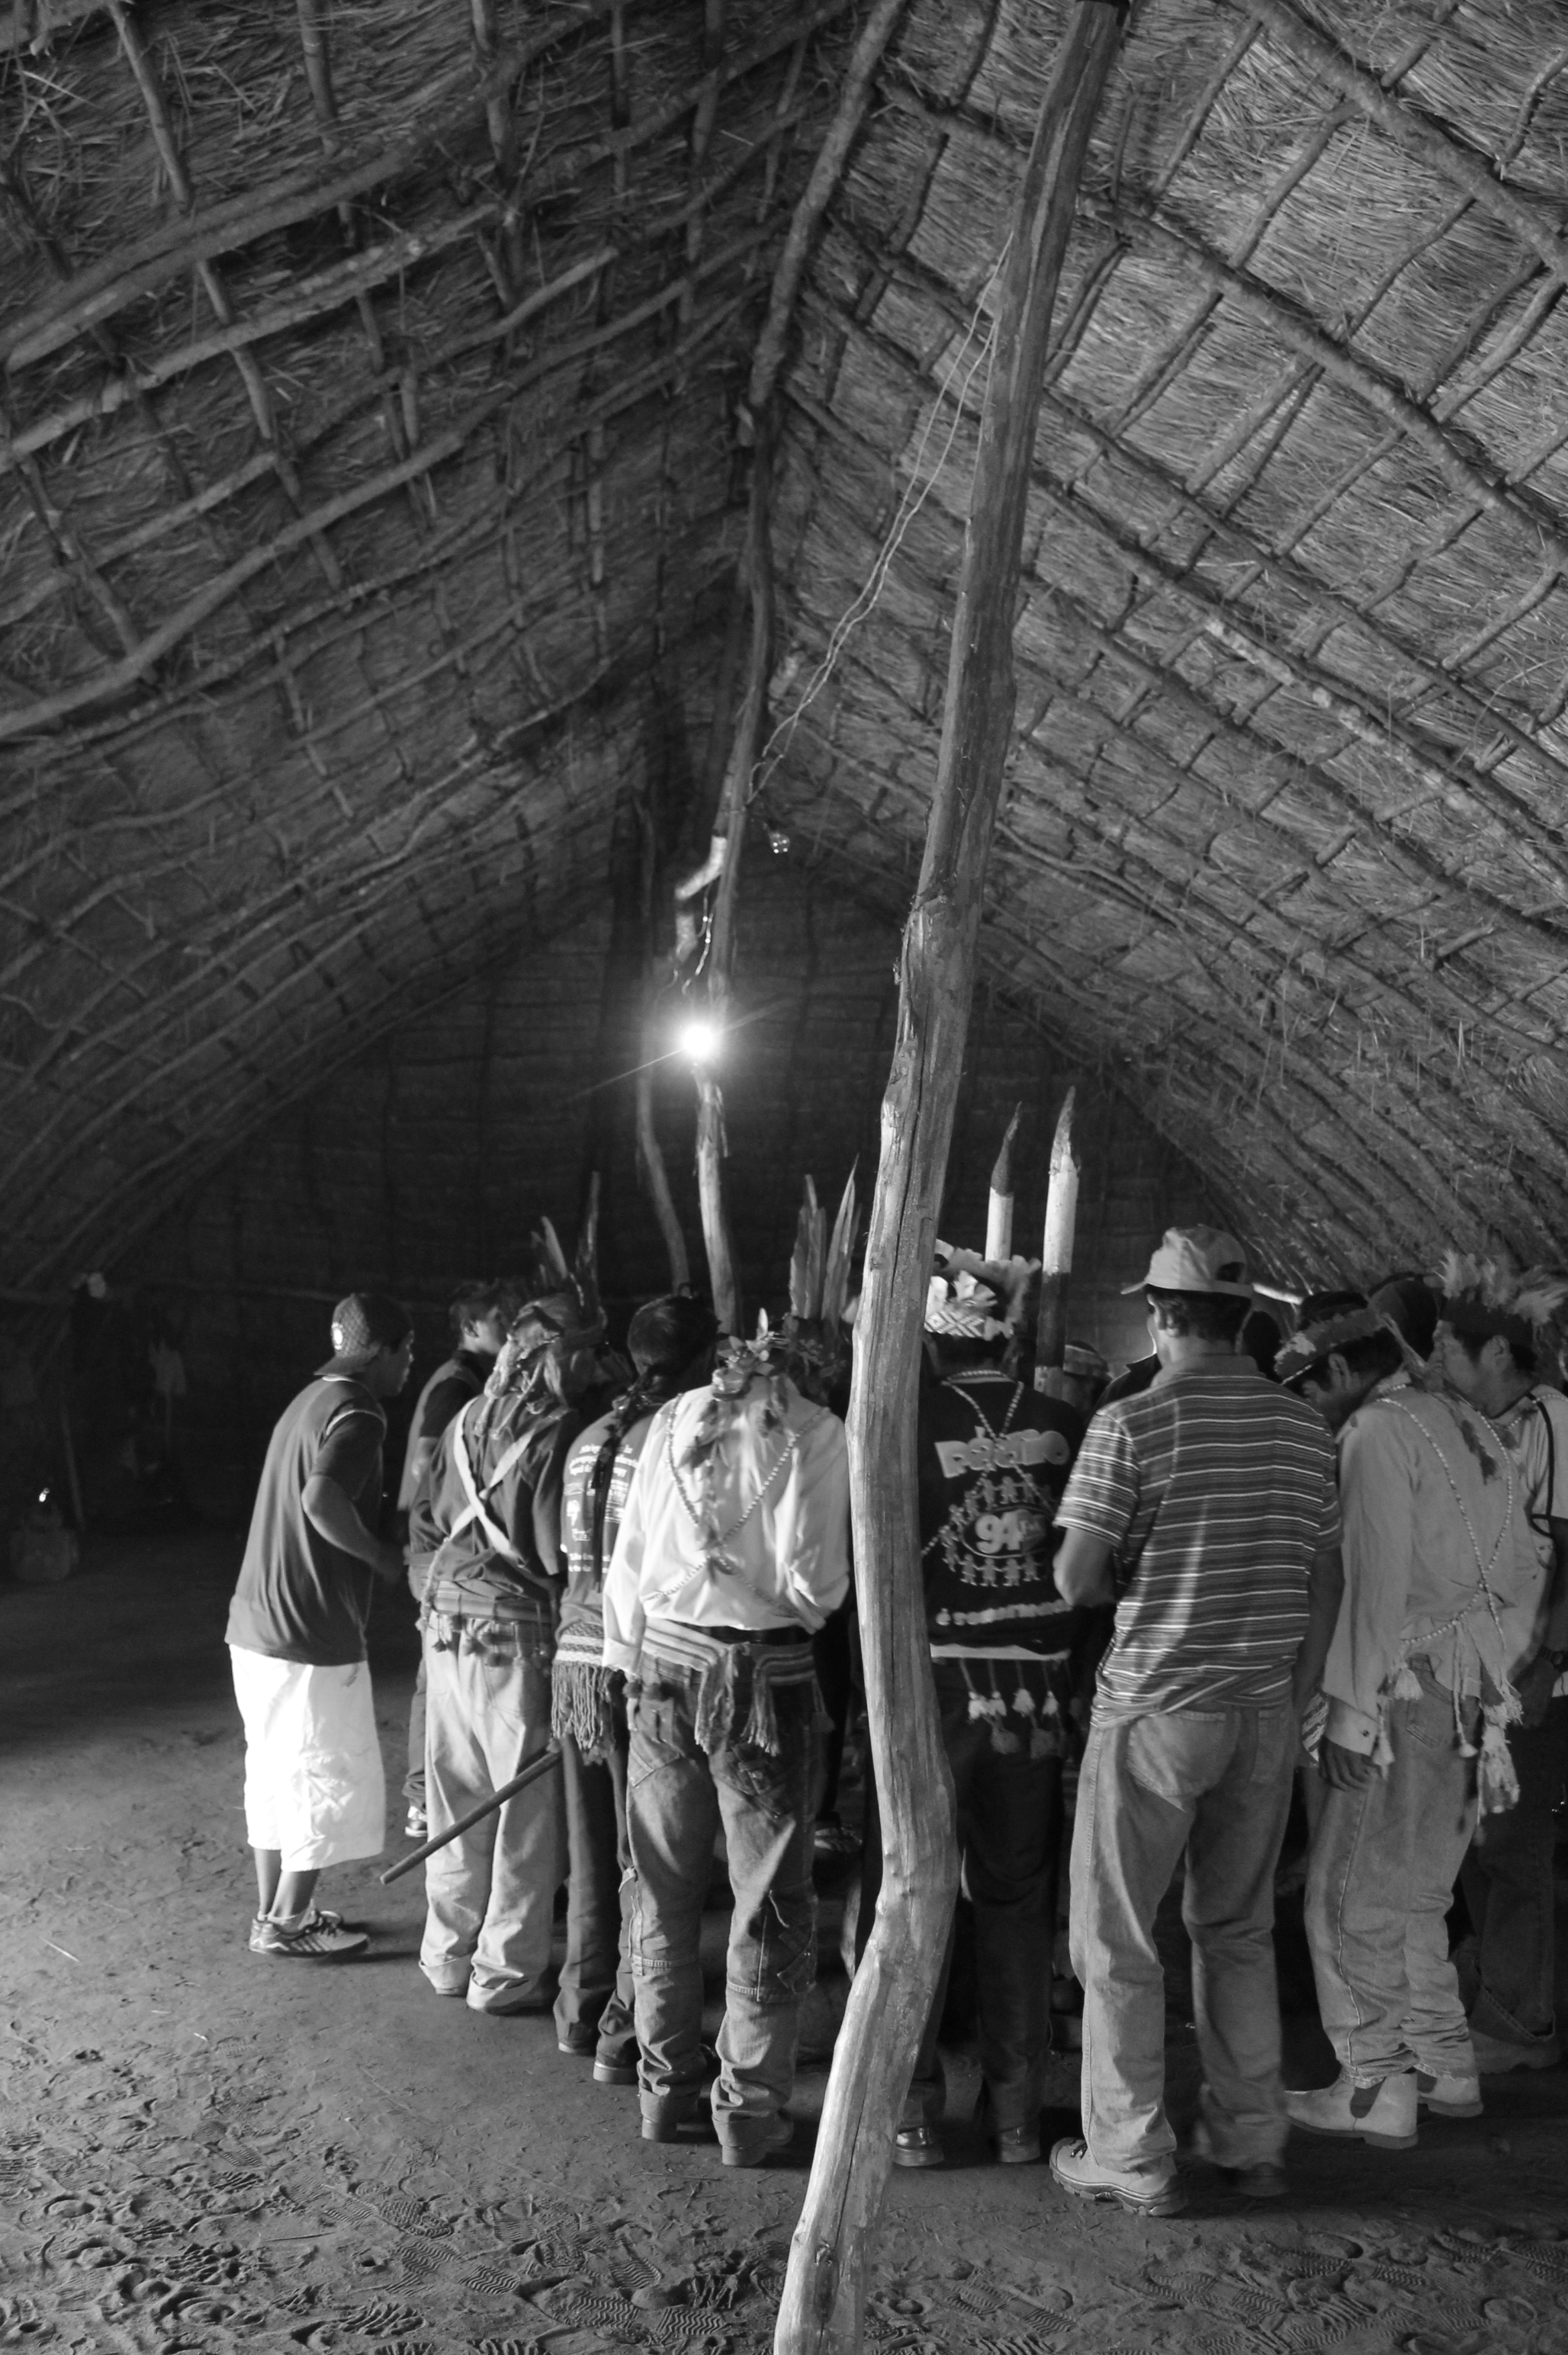
\includegraphics[width=4.9453in,height=7.4272in]{livroredesguaranifinal-img6.jpg}
 

Inaugura\c{c}\~ao de~ogapysy~(casa de reza) kaiowa na Reserva Ind\'igena
Caarap\'o, Caarap\'o (MS). Foto: Tatiane Klein, 2012.

Mobilidade, modalidades de assentamentos e formas organizacionais entre
os Kaiow\'a e Guarani em MS

Levi Marques Pereira\footnote{* Docente na Universidade Federal da
Grande Dourados, pesquisador da FUNDECT e bolsista do CNPq.} 

A mobilidade espacial sempre foi uma caracter\'istica destacada na
bibliografia dos povos de l\'ingua e cultura guarani. O presente artigo
procura identificar e descrever algumas formas de mobilidade entre os
Kaiow\'a e Guarani que vivem em MS, considerando as estrat\'egias por
eles desenvolvidas para, nas circunst\^ancias hist\'oricas atuais,
produzirem seus assentamentos de modo compat\'ivel com seus m\'odulos
organizacionais e concep\c{c}\~oes sociocosmol\'ogicas. O artigo
apresenta algumas caracter\'isticas das modalidades de assentamento
consideradas como tradicionais e outras de desenvolvimento recente.
Estas \'ultimas emergem como respostas adaptativas e criativas desses
coletivos frente \`as profundas transforma\c{c}\~oes hist\'oricas e
econ\^omicas por que passou o ambiente em que vivem, ao recolhimento
compuls\'orio da maior parte da popula\c{c}\~ao em reservas\footnote{
Entre 1915 e 1928 o SPI demarcou oito pequenas \'areas. Naquele momento
os documentos denominaram esses espa\c{c}os de reservas, onde depois
foram implantados postos ind\'igenas, destinados ao recolhimento da
popula\c{c}\~ao de in\'umeras comunidades. Nas formula\c{c}\~oes
correntes entre regionais e ind\'igenas at\'e hoje esses espa\c{c}os
s\~ao denominados como reserva, embora jur\'idica e administrativamente
sejam reconhecidos como terras ind\'igenas.\par } e aos processos de
degrada\c{c}\~ao da paisagem natural, cada vez mais intensos.

Viveiros de Castro, no texto de apresenta\c{c}\~ao da edi\c{c}\~ao
brasileira do livro de Nimuendaju (1987: xxiii), afirma que os Guarani
{\textquotedblleft}continuam cheios de mist\'erio, pela complexidade de
sua cultura, sua espantosa capacidade de desterritorializa\c{c}\~ao ---
que sugere um descolamento entre a sociedade e qualquer suporte
morfol\'ogico est\'avel, apontando talvez a l\'ingua como o locus da
{\textquoteleft}persevera\c{c}\~ao do ser{\textquoteright}
Guarani{\textquotedblright}. Considero que essa suposta
{\textquotedblleft}espantosa capacidade de
desterritorializa\c{c}\~ao{\textquotedblright} tem recebido muita
\^enfase nos estudos sobre os Mbya cujas etnografias t\^em influenciado
a maior parte das s\'inteses te\'oricas, em detrimento dos estudos
sobre os Kaiow\'a e Guarani que vivem em MS. 

Nas \'ultimas d\'ecadas a etnografia dos Kaiow\'a e Guarani enfatiza com
intensidade crescente os v\'inculos hist\'oricos entre determinados
coletivos humanos e espa\c{c}os espec\'ificos, por eles denominado de
tekoha. Tal \^enfase pode estar relacionada \`a impossibilidade
hist\'orica de seguir praticando seu modo pr\'oprio de deslocamento de
fam\'ilias e coletividades, oguata, devido \`a ocupa\c{c}\~ao das
terras por propriedades particulares. O oguata, movimento orientado
para o estabelecimento de assentamentos nos quais seria poss\'ivel
recomposi\c{c}\~ao da harmonia nas rela\c{c}\~oes intracomunit\'arias,
intercomunit\'arias e entre humanos e as divindades, foi substitu\'ido
por outro movimento, o sarambipa, que resulta da inquieta\c{c}\~ao
constante, produzida pela simultaneidade na necessidade de deslocamento
e a impossibilidade de se dispor de espa\c{c}os nos quais os coletivos
possam se recompor com grau satisfat\'orio de estabilidade e harmonia.
Nesse sentido, considero que a etnografia sobre os Kaiow\'a e Guarani
pode contribuir para a discuss\~ao do tema da mobilidade entre os povos
guarani, sendo o presente texto uma contribui\c{c}\~ao para tal debate.
Nosso objetivo aqui \'e demonstrar como os Kaiow\'a e Guarani produzem
modalidades de assentamentos e formas de mobilidade espacial no
movimento de reprodu\c{c}\~ao de suas comunidades, processo que se
realiza em ambiente extremamente adverso.

A diversidade e complexidade das formas de assentamento foi amplamente
discutida na arqueologia e em estudos de ecologia cultural. O presente
artigo se restringe a uma abordagem antropol\'ogica, com \^enfase na
organiza\c{c}\~ao social. Na arqueologia os assentamentos s\~ao
entendidos como o espa\c{c}o onde vivem os membros de um coletivo
humano, incluindo a\'i as \'areas necess\'arias \`a realiza\c{c}\~ao de
fun\c{c}\~oes produtivas, sociais e culturais que asseguram sua
reprodu\c{c}\~ao de determinado coletivo humano (Beber, 2004: 132-3;
Cavalcante, 2013: 64-ss). Essa defini\c{c}\~ao arqueol\'ogica n\~ao \'e
rigorosamente aplicada \`a presente descri\c{c}\~ao. Tento aqui
evidenciar como as atuais formas de assentamento kaiow\'a e guarani
s\~ao transformadas pela precariedade e escassez de recursos ambientais
e outros, o que imp\~oe a circula\c{c}\~ao fora do espa\c{c}o de
resid\^encia para desenvolverem uma s\'erie de atividades voltadas para
a satisfa\c{c}\~ao das necessidades cotidianas mais elementares. 

De import\^ancia fundamental para a presente discuss\~ao \'e o conceito
de {\textquotedblleft}confinamento{\textquotedblright} em reservas,
desenvolvido por Brand (1997). A esse conceito, proponho acrescentar a
percep\c{c}\~ao das reservas enquanto {\textquotedblleft}\'areas de
acomoda\c{c}\~ao\footnote{ A ideia de acomoda\c{c}\~ao ganhou destaque
na antropologia do contato produzida nos anos 60 e 70, com Cardoso de
Oliveira (1972 [1964]), entre outros. No presente texto o uso \'e
complementando, pois o esfor\c{c}o \'e destacar as pr\'oprias
formula\c{c}\~oes dos Kaiow\'a e Guarani da experi\^encia de
recolhimento compuls\'orio em pequenas por\c{c}\~oes de terras,
demarcadas como reservas e atualmente denominadas de terras
ind\'igenas. }{\textquotedblright}. As reservas estariam na base da
gera\c{c}\~ao de novas figura\c{c}\~oes sociais kaiow\'a e guarani,
caracterizadas pelo desenvolvimento de novas formas de mobilidade e
tipologias de assentamento. Nesse novo cen\'ario, realiza-se uma
s\'erie de pr\'aticas voltadas para a contingente acomoda\c{c}\~ao ao
entorno regional. Acomoda\c{c}\~ao tem aqui o sentido de
constru\c{c}\~ao de um arranjo, sempre prec\'ario, assim\'etrico e
transit\'orio, entre as institui\c{c}\~oes e pr\'aticas sociais
ind\'igenas e as ag\^encias da sociedade nacional.

Paralelamente ao movimento de acomoda\c{c}\~ao \'e poss\'ivel
identificar pr\'aticas que v\~ao na dire\c{c}\~ao oposta, da n\~ao
acomoda\c{c}\~ao, da recusa de assimetria e da busca de reposi\c{c}\~ao
da autonomia ind\'igena. Nas \'ultimas d\'ecadas surgiram formas de
mobilidade e modalidades de assentamento que n\~ao est\~ao diretamente
associadas \`as reservas. Para discutir esse movimento, apresento a
configura\c{c}\~ao hist\'orica e sociol\'ogica das reservas, dos
acampamentos mobilizados para a retomada de terras de ocupa\c{c}\~ao
tradicional e de grupos de fam\'ilias que vivem em periferias de
cidades. Entretanto, seria poss\'ivel identificar outras modalidades de
assentamento e formas de mobilidade, que n\~ao ser\~ao tratadas aqui,
dada a limita\c{c}\~ao do espa\c{c}o. 

Antecedentes

Antes da ocupa\c{c}\~ao agropecu\'aria do sul de MS, o que se deu de
modo gradual a partir da pen\'ultima d\'ecada do s\'eculo XIX, os
Kaiow\'a e Guarani ocupavam um territ\'orio comum, tet\~a, onde se
distribu\'iam as aldeias, tekoha, por sua vez, compostas por uma
m\'edia de tr\^es a cinco parentelas, te{\textasciiacute}yi. Cada
parentela dispunha de uma por\c{c}\~ao de terra de uso exclusivo para o
desenvolvimento de suas atividades produtivas e rituais cotidianas. Os
tekoha estavam inseridos em redes de alian\c{c}as mais amplas, de
car\'ater pol\'itico e, principalmente, religioso (Meli\'a, Gr\"unberg
\& Gr\"unberg, 1976; Pereira, 2004), efetivadas em momentos especiais.
Em termos gerais, a maior parte das comunidades logrou manter sua
autonomia organizacional e a posse de suas terras at\'e meados do
s\'eculo XX.

As oito reservas, demarcadas pelo SPI entre 1915 e 1928, perfazendo um
total de menos de 19 mil hectares, foram projetadas para o recolhimento
de um grande n\'umero de comunidades que viviam dispersas pelo
territ\'orio. Assim, a reserva deveria cumprir a fun\c{c}\~ao
pol\'itica de liberar as terras para a especula\c{c}\~ao imobili\'aria
e posterior ocupa\c{c}\~ao agropecu\'aria. 

Os Kaiow\'a e Guarani resistiram de diversas formas, procurando manter a
posse das terras que ocupavam. Entretanto, a quase totalidade das
comunidades gradativamente teve de ceder \`as press\~oes dos
fazendeiros e dos funcion\'arios do SPI e se recolher nas reservas. O
deslocamento territorial implicou na dispers\~ao das fam\'ilias e no
enfraquecimento dos v\'inculos de sociabilidade que cimentavam as
rela\c{c}\~oes inter e extracomunit\'arias. Essa dispers\~ao \'e
denominada pelos ind\'igenas de sarambipa ou esparramo, e pode ser
percebida como uma categoria temporal que separa o tempo antigo, yma
guare, quando as comunidades dispunham de autonomia, e o tempo atual,
ara pyahu, caracterizado pela retomada de seus tekoha e autonomia
organizacional. A expuls\~ao das comunidades de seus espa\c{c}os de
ocupa\c{c}\~ao tradicional durou d\'ecadas e est\'a em curso at\'e
hoje. Resulta da\'i que atualmente as reservas apresentem grande
densidade demogr\'afica, fato agravado pelo significativo crescimento
vegetativo da popula\c{c}\~ao.

Os pr\'oprios Kaiow\'a e Guarani reconhecem que a vida em reserva
dificulta a realiza\c{c}\~ao das pr\'aticas socioculturais
desenvolvidas nas figura\c{c}\~oes sociais de seus antigos
assentamentos de ocupa\c{c}\~ao tradicional. Por outro lado, seguem se
reconhecendo como Kaiow\'a ou como Guarani, praticantes de formas de
convivialidade particulares, diretamente relacionadas ao seu modo
pr\'oprio de ser, ava reko. Em certo sentido, as novas modalidades de
assentamento podem ser entendidas como respostas adaptativas a essa
nova condi\c{c}\~ao. Os l\'ideres de parentela buscam dispor de novos
instrumentos culturais e habilidades que lhes permitam orientar sua
criatividade para efetivarem a exist\^encia de seus coletivos, ou como
denominam, levantar a comunidade, opu{\textasciiacute}\~a che
re{\textasciiacute}yi kuera.

A reserva como \'area de confinamento e de acomoda\c{c}\~ao e a
gera\c{c}\~ao de novas formas de mobilidade e assentamentos

J\'a na publica\c{c}\~ao de Aspectos fundamentais da cultura guarani,
datada de 1962, Schaden utiliza a id\'eia de confinamento, quando
afirma que os Guarani {\textquotedblleft}j\'a n\~ao ocupam \'areas
extensas e concretas, mas est\~ao confinados a pequenas reservas ou
aldeias sob prote\c{c}\~ao ou mesmo administra\c{c}\~ao
oficial{\textquotedblright} (Schaden, 1974: 10, grifos meus). Mas foi
Brand (1997) quem desenvolveu o conceito na forma como ele passou a ser
usado pela maior parte dos pesquisadores.

A situa\c{c}\~ao de reserva alterou profundamente o padr\~ao tradicional
de assentamento das parentelas e aldeias. Antes da ocupa\c{c}\~ao
colonial, os assentamentos se orientavam pelas seguintes
caracter\'isticas: a) disponibilidade de locais considerados
apropriados, por comportarem recursos naturais para o estabelecimento
de resid\^encia, pois, como disse um l\'ider pol\'itico,
{\textquotedblleft}antigamente o \'indio sempre procurava o lugar bom
para morar, onde tinha mato bom, \'agua boa{\textquotedblright}, ou
seja, fatores ecol\'ogicos influenciavam na escolha; b) o local estar
livre de amea\c{c}as sobrenaturais, como esp\'iritos perigosos; c)
proximidade de parentelas aliadas, necess\'arias para as pr\'aticas
matrimoniais, festivas e rituais; d) a capacidade do casal de
{\textquotedblleft}cabe\c{c}as{\textquotedblright} de parentela de
conduzir eficazmente a vida comunit\'aria, ou seja, de demonstrar
habilidade para unir os parentes e resolver problemas de conviv\^encia;
e, ainda, e) a n\~ao incid\^encia de doen\c{c}as ou de mortes
repentinas provocadas por causas consideradas ruins, paje vai.

As caracter\'isticas acima apontadas orientavam a mobilidade dos
assentamentos dentro do territ\'orio de ocupa\c{c}\~ao tradicional,
sendo os deslocamentos normalmente orientados pelo prop\'osito de
resolu\c{c}\~ao de conflitos, recomposi\c{c}\~ao de alian\c{c}as e
surgimento de nova parentela. Naquele cen\'ario, a maior ou menor
proximidade social e espacial entre as parentelas estava conectada a
fatores ambientais, sociol\'ogicos e cosmol\'ogicos. A ocupa\c{c}\~ao
agropastorial interrompeu essa din\^amica de mobilidade, que
poder\'iamos denominar de tradicional, oguata por\~a, e imp\^os um novo
tipo de deslocamento, o sarambipa ou esparramo, que tem ainda o sentido
de conflito e confus\~ao. O recolhimento das comunidades nas reservas
instituiu espa\c{c}os de produ\c{c}\~ao das novas rela\c{c}\~oes
sociais, interferindo em todos os campos da vida das pessoas a\'i
reunidas. A reserva \'e um espa\c{c}o amb\'iguo j\'a que por um lado
obriga a proximidade f\'isica entre parentelas (confinamento), mas por
outro lado, tais rela\c{c}\~oes de vizinhan\c{c}as s\~ao impostas e
muitas vezes se \'e obrigado a conviver com desafetos, o que gera
infind\'aveis tens\~oes, conflitos, mal-estar social e
fragmenta\c{c}\~ao do tecido social, caracter\'isticas associadas ao
sarambipa e ao modo impr\'oprio de se viver, teko vai.

A compreens\~ao da complexa situa\c{c}\~ao criada nas reservas desafia
pesquisadores (inclusive ind\'igenas). A contribui\c{c}\~ao mais
significativa foi a de Brand (1997), com desenvolvimento do conceito de
confinamento, entendido como o processo de recolhimento for\c{c}ado de
in\'umeras comunidades em reservas diminutas, o que leva a
sobreposi\c{c}\~ao de comunidades no mesmo espa\c{c}o. O conceito de
confinamento inspirou pesquisadores a tentarem abordagens alternativas.
Do meu pr\'oprio ponto de vista, estou propenso a considerar a id\'eia
de \'area de acomoda\c{c}\~ao como bastante apropriada para expressar
alguns aspectos das configura\c{c}\~oes sociais originadas a partir da
imposi\c{c}\~ao da reserva como modelo oficial de assentamento,
diretamente imposto pelo Estado brasileiro. 

Pensar a reserva como \'area de acomoda\c{c}\~ao requer a
descri\c{c}\~ao de aspectos de natureza pol\'itica e sociol\'ogica
presentes nos processos sociais vividos nessa nova experi\^encia
hist\'orica. A situa\c{c}\~ao de reserva deve ser pensada ainda como
experi\^encia criativa, nela os ind\'igenas mobilizam os referenciais e
recursos dispon\'iveis, pr\'oprios ou introduzidos, para produzirem
formas organizacionais capazes de tornar vi\'avel a sobreviv\^encia
f\'isica e a constru\c{c}\~ao de figura\c{c}\~oes sociais que, de
alguma maneira, assegurem a continuidade de sua forma\c{c}\~ao social. 

A experi\^encia hist\'orica de viver em pequenas terras se reflete em
transforma\c{c}\~oes profundas na vida social das comunidades que
perderam suas terras. Tornou invi\'avel a autonomia para gerir a maior
parte do cotidiano de sua vida econ\^omica, pol\'itica e religiosa. As
figura\c{c}\~oes sociais articuladas nas reservas passam a reunir
comunidades que antes n\~ao interagiam em car\'ater permanente. Isto
gera uma s\'erie de problemas organizacionais novos, para os quais o
modelo de organiza\c{c}\~ao social at\'e ent\~ao praticado nem sempre
disp\~oe de instrumentos apropriados para dar respostas imediatas. O
cen\'ario da reserva a presen\c{c}a necess\'aria das ag\^encias e
outros sujeitos sociais pertencentes \`a sociedade nacional. A \'area
de acomoda\c{c}\~ao se transforma em um cen\'ario inter\'etnico de
intera\c{c}\~ao permanente.

Nas pequenas terras ind\'igenas que lhes foram reconhecidas os Kaiow\'a
e Guarani vivenciam limita\c{c}\~oes na operacionaliza\c{c}\~ao das
t\'ecnicas de produ\c{c}\~ao material, do sistema de cuidados com a
sa\'ude e das pr\'aticas festivas e rituais. No rastro dos novos
problemas ocorre a presen\c{c}a permanente de institui\c{c}\~oes
prestadoras de servi\c{c}o, como a Miss\~ao Evang\'elica Caiu\'a (desde
1928), do SPI/FUNAI (desde a d\'ecada de 1920) e, a partir da d\'ecada
de 1970, de v\'arias outras ag\^encias governamentais e da sociedade
civil. Essas institui\c{c}\~oes passaram a exercer import\^ancia
crescente no oferecimento de servi\c{c}os e na defini\c{c}\~ao da
din\^amica de vida das popula\c{c}\~oes reservadas.

Por conseguinte, a presen\c{c}a dessas institui\c{c}\~oes colocou \`a
disposi\c{c}\~ao dos Kaiow\'a e Guarani mecanismos de exerc\'icio da
pol\'itica at\'e ent\~ao inusitados. A interfer\^encia nas formas de
composi\c{c}\~ao de alian\c{c}as entre as parentelas das diversas
comunidades recolhidas nas reservas passa a ser direta e cont\'inua. Em
muitos casos os agentes externos assumem a atribui\c{c}\~ao de agir
como dirigentes dos processos pol\'iticos internos. Essa
atribui\c{c}\~ao \'e flagrante no caso do chefe de posto do SPI/FUNAI,
figura central nessa nova configura\c{c}\~ao at\'e a d\'ecada de 1980.
As decis\~oes sobre diversos assuntos referentes \`a vida pol\'itica
das comunidades reservadas passam a ser tomadas com relativa
independ\^encia e {\textquotedblleft}neutralidade{\textquotedblright}
em rela\c{c}\~ao \`as formas de exerc\'icio da pol\'itica kaiow\'a e
guarani. Os agentes indigenistas n\~ao orientam sua atua\c{c}\~ao pela
l\'ogica interna da organiza\c{c}\~ao social das comunidades, at\'e
porque, na maioria das vezes, n\~ao entendem como isso se d\'a, ou
mesmo porque as pr\'aticas aut\'octones se chocam com os interesses de
suas institui\c{c}\~oes. Percebendo esse novo cen\'ario pol\'itico,
n\~ao foram raros os casos de lideran\c{c}as que passaram a recorrer a
esses agentes na busca do estabelecendo alian\c{c}as estrat\'egicas,
por eles identificadas como ben\'eficas \`a sua pr\'opria parentela ou
comunidade.

Muitas lideran\c{c}as que passaram a viver nas reservas nem sempre
dispunham de referenciais apropriados para lidar com os novos problemas
originados na \'area de acomoda\c{c}\~ao. Recorrer ao mission\'ario, ao
administrador ou ao indigenista parecia a solu\c{c}\~ao mais apropriada
ou a \'unica forma de administrar conflitos. Essas novas modalidades de
exerc\'icio da pol\'itica implicaram na perda de prest\'igio das
lideran\c{c}as identificadas como tradicionais, principalmente daquelas
cujo reconhecimento estava baseado em pr\'aticas religiosas, sendo
raros os casos dos grandes xam\~as que n\~ao viram seu prest\'igio
seriamente desgastado. Por esse motivo, muitos xam\~as dizem que na
reserva {\textquotedblleft}ficamos encostados e esquecidos, ningu\'em
lembra mais de n\'os{\textquotedblright}, ou seja, sem fun\c{c}\~ao na
configura\c{c}\~ao a\'i institu\'ida.

O campo gerencial formado pelas ag\^encias indigenistas passa a fazer
parte do cen\'ario total de intera\c{c}\~ao consolidado nas reservas.
\'E buscando a capacita\c{c}\~ao para atuar nesse cen\'ario que as
lideran\c{c}as procurar\~ao construir as condi\c{c}\~oes de viabilidade
para seguirem reproduzindo suas comunidades. Isto porque a reserva
apresenta novas caracter\'isticas demogr\'aficas, econ\^omicas, sociais
e pol\'iticas. Os l\'ideres das parentelas procurar\~ao novos canais de
legitima\c{c}\~ao e fortalecimento pol\'itico, uma vez que as
configura\c{c}\~oes das antigas redes se tornam, em muitos casos,
inoperantes ou ineficientes para articular respostas aos novos
problemas. 

Qualquer chefe de posto da Funai, agente indigenista, mission\'ario, ou
mesmo dono de venda, contratante de m\~ao de obra, taxista, etc., que
tenha convivido algum tempo com lideran\c{c}as de uma reserva kaiow\'a
e guarani, costuma relatar eventos nos quais foi solicitado a opinar ou
atuar como mediador em conflitos internos. Na maioria das vezes, esses
agentes n\~ao disp\~oem da m\'inima condi\c{c}\~ao para compreender os
fundamentos das demandas para as quais foram instigados a opinar ou
atuar e, muito menos, dimensionar as apropria\c{c}\~oes internas a que
a sua interfer\^encia estar\'a sujeita. Isto demonstra a \^ansia das
lideran\c{c}as em disporem de referenciais para lidar com o cen\'ario
da reserva e a din\^amica das rela\c{c}\~oes a\'i institu\'idas, que
dissolvem e tornam ineficiente o modo como tradicionalmente articularam
suas comunidades. 

Deslocar-se da reserva para escapar de conflitos pol\'iticos ficou cada
vez mais dif\'icil com a ocupa\c{c}\~ao agropecu\'aria de toda a
regi\~ao, limitando a realiza\c{c}\~ao do oguata em \'areas de
ref\'ugio, movimento que foi muito presente at\'e a d\'ecada de 1960.
Assim, a busca de entendimento com os agentes externos que controlam as
reservas passa a ser, at\'e certo ponto, a sa\'ida mais viabilizar a
conviv\^encia em grandes ajuntamentos de parentelas. 

Na reserva, os l\'ideres das parentelas n\~ao relutam em procurar as
{\textquotedblleft}autoridades{\textquotedblright} --- como denominam o
Capit\~ao e o Chefe de Posto\footnote{ Chefe de Posto era o
funcion\'ario do \'org\~ao indigenista respons\'avel por gerir a
reserva e o Capit\~ao era o \'indio escolhido como l\'ider pol\'itico
da reserva, cuja nomea\c{c}\~ao era realizada por representante do
\'org\~ao indigenista oficial. Nos \'ultimos anos a Funai destituiu a
figura do chefe de posto, nas os \'indios seguem chamando os
funcion\'arios da Funai de chefe e nutrindo a expectativa de que atuem
enquanto tal, mas costumam dizer que a Funai agora \'e mais
{\textquotedblleft}mansa{\textquotedblright}, o que remete ao
autoritarismo dos antigos chefes.} e outros atores que os
substitu\'iram ou surgiram com a prolifera\c{c}\~ao de ag\^encias
indigenistas --- para a resolu\c{c}\~ao de conflitos internos, cobrando
deles o exerc\'icio das atribui\c{c}\~oes institucionais das quais
imaginam estarem investidas. A preocupa\c{c}\~ao fundamental \'e
assegurarem que atuem a favor de seus grupos pol\'iticos particulares.
Nesse sentido, tende a existir uma disputa pelo
{\textquotedblleft}aprisionamento{\textquotedblright} das autoridades,
numa esp\'ecie de manipula\c{c}\~ao rec\'iproca e oscilante.

Os recursos disponibilizados em programas de sa\'ude,
escolariza\c{c}\~ao,
{\textquotedblleft}desenvolvimento{\textquotedblright} agr\'icola e
evangeliza\c{c}\~ao consolidaram e deram sustenta\c{c}\~ao ao novo
formato de rela\c{c}\~oes econ\^omicas, pol\'iticas e sociais nas
reservas. Os Kaiow\'a e Guarani se apropriaram da presen\c{c}a de tais
programas para criarem as condi\c{c}\~oes de viabilidade de suas
figura\c{c}\~oes sociais nas reservas, mesmo em car\'ater prec\'ario.
Pode-se identificar um esfor\c{c}o das lideran\c{c}as no sentido de
transformar a reserva em {\textquotedblleft}aldeia{\textquotedblright}
ou tekoha (enquanto espa\c{c}o de produ\c{c}\~ao do modo pr\'oprio de
ser). Com perd\~ao pelo abuso lingu\'istico, procuravam
{\textquotedblleft}tekoharizar{\textquotedblright} a reserva. Por um
lado, esse movimento implica em concess\~oes e esfor\c{c}os de
adequa\c{c}\~ao ao cen\'ario da reserva, mas por outro comporta
espa\c{c}os de ag\^encia ind\'igena (agency), de subvers\~ao,
inova\c{c}\~ao, altera\c{c}\~ao e empenho em reorientar programas
implantados pelas ag\^encias indigenistas, no esfor\c{c}o em assegurar
o atendimento de pautas pr\'oprias aos coletivos ind\'igenas que vivem
na reserva.  

For\c{c}ados a viverem em reservas e impossibilitados de seguirem
vivendo em parentelas dispersas, segundo a configura\c{c}\~ao de redes
de alian\c{c}as com uma fisionomia hist\'orica e flex\'ivel, os
Kaiow\'a e Guarani se viram cada vez mais enredados na depend\^encia
dos recursos e servi\c{c}os das ag\^encias indigenistas. Al\'em do
confinamento espacial, a reserva se constitui num ambiente de
experimento de novas pr\'aticas culturais. Isto permite apreender esse
espa\c{c}o como \'area de acomoda\c{c}\~ao dos ind\'igenas ao sistema
sociocultural nacional.

Na segunda e terceira d\'ecada do s\'eculo XX, per\'iodo em que se
demarcou pequenas \'areas destinadas \`a ocupa\c{c}\~ao ind\'igena, as
a\c{c}\~oes promovidas pelo SPI tinham o objetivo de manter o controle
da popula\c{c}\~ao e conduzi-la ao que se imaginava ser a
integra\c{c}\~ao plena \`a sociedade nacional. Acontece que todo esse
planejamento n\~ao surtiu o resultado esperado. A integra\c{c}\~ao
n\~ao se efetivou da maneira como foi idealizada pelas
institui\c{c}\~oes indigenistas. Ao longo das d\'ecadas, as pol\'iticas
voltadas para a popula\c{c}\~ao ind\'igena passaram por revis\~oes e
adequa\c{c}\~oes. A Constitui\c{c}\~ao de 1988 p\^os fim \`a
orienta\c{c}\~ao assimilacionista, definindo o respeito \`a diversidade
cultural como o paradigma que deveria orientar todas as a\c{c}\~oes
indigenistas do Estado e da sociedade civil. 

A mudan\c{c}a no plano legal teve impacto no surgimento de novas
modalidades de assentamentos, discutidas adiante. No plano da
a\c{c}\~ao institucional, a mudan\c{c}a de paradigma n\~ao surtiu,
at\'e o momento, todos os efeitos e consequ\^encias esperadas.
Prefeituras e secretarias de estado n\~ao conseguem implantar
servi\c{c}os diferenciados e adequados \`as caracter\'isticas culturais
dos ind\'igenas. Ocorrem ainda constantes investidas contra os direitos
ind\'igenas, promovidas por setores da sociedade nacional que se
consideram prejudicados pela legisla\c{c}\~ao atual, o que p\~oe em
risco a continuidade desses direitos. Em MS, s\~ao frequentes os casos
de \'org\~aos governamentais e da sociedade civil que confrontam
abertamente os direitos assegurados na Constitui\c{c}\~ao.

Nas pequenas terras ind\'igenas as parentelas menos influentes ficam
obrigadas a se sujeitar \`a domina\c{c}\~ao dos l\'ideres pol\'iticos
das parentelas politicamente mais fortes, por serem origin\'arias ou
mais antigas na reserva, ou ainda por terem estabelecido alian\c{c}as
preferenciais com ag\^encias externas. Explicando os motivos que
levaram sua comunidade a retornar para Guyra Rok\'a em 2002, o l\'ider
dessa comunidade afirmou que {\textquotedblleft}na terra (reserva)
demarcada a gente entra sem direito a nada, se vai plantar tem que
pedir autoriza\c{c}\~ao para o pessoal de l\'a, al\'em disso, \'e
sempre criticado{\textquotedblright}. Assim, a comunidade deslocada de
seu territ\'orio vive sob uma completa sujei\c{c}\~ao pol\'itica. Os
recursos s\~ao sempre monopolizados pelos grupos politicamente mais
fortes, articulados e antigos no local. Quanto mais a popula\c{c}\~ao
se adensa, mais aparecem acusa\c{c}\~oes e conflitos de toda ordem. Por
esse motivo, o cotidiano das reservas mais populosas \'e marcado por
rela\c{c}\~oes conflituosas entre parentelas. Os estabelecidos est\~ao
sempre lembrando os outsiders de sua condi\c{c}\~ao de
{\textquotedblleft}estrangeiros{\textquotedblright}. 

Pelos padr\~oes de organiza\c{c}\~ao social kaiow\'a e guarani, a
conviv\^encia entre distintas parentelas \'e tradicionalmente marcada
pela polariza\c{c}\~ao entre alian\c{c}a e rivalidade pol\'itica.
Historicamente, as parentelas aliadas residiam pr\'oximo umas das
outras, numa dist\^ancia aproximada entre cinco e vinte quil\^ometros,
o que favorecia interc\^ambio matrimonial e religioso. Essa proximidade
expressava coes\~ao social e solidariedade pol\'itica, configurando o
que a literatura denomina de tekoha e tekoha guasu. A conviv\^encia com
as parentelas que estavam fora desse c\'irculo era marcada,
predominantemente, pela hostilidade. Caso ocorressem conflitos que
n\~ao se encaminhassem para uma solu\c{c}\~ao dentro de uma rede de
aliados, a sa\'ida mais prov\'avel era a mudan\c{c}a de um dos grupos
envolvidos no conflito.

Os problemas sociais enfrentados nas reservas t\^em sua origem na
conforma\c{c}\~ao artificial da popula\c{c}\~ao a\'i radicada, o que
implica em muitas tens\~oes devido \`a sobreposi\c{c}\~ao de parentelas
em espa\c{c}o ex\'iguo, disputas pol\'iticas e por recursos escassos.
As reservas tornaram insuficientes os mecanismos de controle social,
baseados em complexos sistemas ideol\'ogico-religiosos. Nessas
circunst\^ancias, a inseguran\c{c}a e a viol\^encia interna atingem
\'indices elevados, levando ao estresse social. Na reserva prosperam o
consumo abusivo de bebidas alco\'olicas e drogas, mortes violentas e
altos \'indices de suic\'idios, fatos intensamente noticiados pela
m\'idia.

As \'areas demarcadas n\~ao suprem todas as necessidades tampouco as
expectativas sociais e econ\^omicas dos Kaiow\'a e Guarani, mas \'e
principalmente nelas que interagem entre si enquanto coletivos
distintos, fazendo incurs\~oes mais ou menos prolongadas no
{\textquotedblleft}mundo do branco{\textquotedblright}, karai reko,
para extrair os bens necess\'arios \`a sua reprodu\c{c}\~ao f\'isica e
cultural. Mesmo na condi\c{c}\~ao de reserva as parentelas procuram
superar com criatividade a imposi\c{c}\~ao de pol\'iticas
assimilacionistas e seguem produzindo sua distintividade coletiva. \'E
claro que num cen\'ario t\~ao complexo e francamente desfavor\'avel,
eles t\^em de conviver com d\'uvidas e incertezas em rela\c{c}\~ao ao
presente e ao futuro de seu modo pr\'oprio de ser. 

A reserva idealizada como \'area de confinamento para promover a
acomoda\c{c}\~ao que permitir\'a a transi\c{c}\~ao do sistema
ind\'igena para o n\~ao ind\'igena acabou por gerar muita
inquieta\c{c}\~ao ou
{\textquotedblleft}incomoda\c{c}\~ao{\textquotedblright} nos
ind\'igenas a\'i recolhidos. Tais dificuldades geram demandas
intermin\'aveis para as ag\^encias p\'ublicas e da sociedade civil que
de alguma forma lhes prestam assist\^encia. A descri\c{c}\~ao das novas
modalidades de assentamentos demonstra a precariedade da
acomoda\c{c}\~ao em reserva e a fal\^encia do indigenismo
assimilacionista. As a\c{c}\~oes foram insuficientes para demover os
Kaiow\'a e Guarani de sua diferencia\c{c}\~ao interna, ao mesmo tempo
em que n\~ao se conformaram com a expropria\c{c}\~ao de suas terras.
Resulta da\'i o empenho das lideran\c{c}as para reaver suas antigas
paragens ou a busca de locais alternativos \`a reserva.

Fam\'ilias kaiow\'a e guarani reacomodadas em periferias de cidades

Muitas fam\'ilias kaiow\'a e guarani passaram pela experi\^encia das
reservas, mas vivem atualmente na periferia de vilas e cidades. Tomarei
como foco de an\'alise algumas fam\'ilias situadas na conflu\^encia de
linhas (estradas vicinais) do munic\'ipio de Vicentina, MS, cujo
levantamento em campo foi realizado durante os estudos de
identifica\c{c}\~ao da terra ind\'igena Guyra Roka (Pereira, 2002). As
linhas separam setores de lotes de terra demarcados com 30 hectares
cada um. Originalmente, o assentamento foi ocupado por pequenos
agricultores que vieram para a regi\~ao a partir de 1943, motivados a
ocupar a Col\^onia Agr\'icola Federal de Dourados, implantada no
governo de Get\'ulio Vargas.

Em alguns desses entroncamentos, como \'e o caso do aqui descrito, se
estabeleceram vendas, resid\^encias, escolas, igrejas, formando
pequenos vilarejos rurais. Com a decad\^encia das pequenas propriedades
familiares, incorporadas a propriedades m\'edias e grandes, a maior
parte da popula\c{c}\~ao migrou para os centros urbanos, deixando para
tr\'as vilas quase fantasmas. A desvaloriza\c{c}\~ao dos lotes urbanos
favoreceu o estabelecimento de fam\'ilias ind\'igenas que perderam
terras na regi\~ao.

A Col\^onia Federal foi implantada sobre parte do territ\'orio
ind\'igena, desarticulando v\'arias comunidades, cuja popula\c{c}\~ao
foi, em sua maioria, deslocada para as reservas. Alguns remanescentes
dessas comunidades n\~ao se adaptaram \`as condi\c{c}\~oes de vida nas
reservas demarcadas e insistiram em permanecer nas proximidades das
terras que historicamente ocupavam, trabalhando como m\~ao de obra
volante nas propriedades agr\'icolas que a\'i se instalaram. Relatos de
v\'arios ind\'igenas apresentam a experi\^encia de vida nas reservas
como traum\'atica. N\~ao dispunham de parentes ou aliados ocupando
posi\c{c}\~oes de prest\'igio nos locais para onde foram transferidos,
tendo sofrido viol\^encias e humilha\c{c}\~oes.

O grupo encontrado no munic\'ipio de Vicentina era liderado por Doraline
e seus filhos, que nasceram na antiga aldeia de Toror\^o, nas
proximidades do c\'orrego Caarap\'o, comunidade vizinha a de Guyra
Roka, munic\'ipio de Caarap\'o. Todos os filhos falam a l\'ingua
guarani e identificam claramente os v\'inculos parentais com segmentos
de popula\c{c}\~ao kaiow\'a que vivem nas reservas de Caarap\'o e
Dourados. Doraline ficou muito feliz em receber not\'icias dos parentes
(atrav\'es do filho de seu primo, que me acompanhava), demonstrando
esperan\c{c}a em retornar o conv\'ivio com os parentes, caso a terra de
Guyra Rok\'a venha a ser assegurada como espa\c{c}o ind\'igena.
Entretanto, n\~ao demonstrou nenhuma inten\c{c}\~ao em se recolher a
alguma das atuais reservas, dada as experi\^encias traum\'aticas a\'i
vividas.

Esse grupo de fam\'ilias vivia \`a margem da assist\^encia social
governamental, em barracos de lona ou madeira reutilizada. Estavam
submetidos \`a constrangedora situa\c{c}\~ao perif\'erica nesses
vilarejos pobres, expostas ao preconceito e mis\'eria, situa\c{c}\~ao a
que foram levadas pelo esbulho de suas terras.

O l\'ider kaiow\'a Ambr\'osio Vilhalva, que me acompanhava na pesquisa
de campo, desabafou:

O que vamos fazer? S\~ao nossos parentes! Agora alguns est\~ao um pouco
misturados com branco, mas vamos aceit\'a-los assim mesmo, eles n\~ao
t\^em culpa de todo esse sofrimento que pesa sobre eles, o que importa
\'e reorganizar a nossa aldeia e retomar a nossa vida. Muita coisa os
rezadores (xam\~as) v\~ao recuperar, mas teremos que conviver com
muitas perdas, n\~ao h\'a como recuperar tudo.

Nas periferias das cidades do sul de MS, grande n\'umero de fam\'ilias
guarani e kaiow\'a vivem em completa condi\c{c}\~ao de precariedade
social, suspeitando de qualquer iniciativa envolvendo
institui\c{c}\~oes p\'ublicas ou inst\^ancias de poder. 

Acampamentos mobilizados para a reocupa\c{c}\~ao da terra --- tekorar\~a

A terceira modalidade de assentamento aqui descrita se refere aos
coletivos mobilizados para a reocupa\c{c}\~ao de terras que consideram
de ocupa\c{c}\~ao tradicional. Geralmente, est\~ao situados: a) em
margens de rodovias nas proximidades da terra reivindicada; b) em
acampamentos no interior das reservas; c) ocupando pequenas
por\c{c}\~oes da terra reivindicada. 

No caso de estarem acampados fora da reserva, os parentes que a\'i
permanecem costumam ajudar a manter os parentes no acampamento, onde
sempre aparecem em visitas que podem durar alguns dias. Existe um
constante fluxo de pessoas que chegam e que saem dos acampamentos,
mantendo a troca de bens e informa\c{c}\~oes. A maior parte das pessoas
que comp\~oem o acampamento \'e relacionada por la\c{c}os de parentesco
com seus principais l\'ideres. Pode acontecer de parte significativa
das pessoas que vivem no acampamento n\~ao estarem vivendo juntas antes
de se reunirem para formar o acampamento. O que cimenta as
rela\c{c}\~oes entre as pessoas que passam a viver juntas no
acampamento \'e o reconhecimento do v\'inculo com a antiga comunidade
que ocupava a terra que est\'a no foco da reivindica\c{c}\~ao. Esse
v\'inculo se d\'a atrav\'es de ancestrais, pais, av\'os, tios etc., que
nasceram no local, e tamb\'em por participarem de redes de alian\c{c}as
matrimoniais, festivas e rituais. 

A dispers\~ao das pessoas \'e resultado dos v\'arios anos que se
passaram entre a expuls\~ao da terra e a decis\~ao de acamparem. No
intervalo da di\'aspora muitas pessoas nasceram, se casaram ou
morreram. \'E comum que s\'o as pessoas com mais de 40 anos tenham
nascido no local e s\'o os velhos com mais de 50 anos mantenham a
lembran\c{c}a das formas de sociabilidade desenvolvidas no local. A
recomposi\c{c}\~ao da hist\'oria da comunidade no per\'iodo anterior
\`a expuls\~ao \'e embasada na hist\'oria contada pelos velhos, nas
conversas nas rodas de terer\'e ou mate. No reencontro dos parentes
atualiza-se a mem\'oria das alian\c{c}as e da conforma\c{c}\~ao social
e pol\'itica da comunidade no per\'iodo anterior \`a expuls\~ao. Tais
mem\'orias fornecem as refer\^encias para a recomposi\c{c}\~ao dos
la\c{c}os societ\'arios que as pessoas que comp\~oem o acampamento
est\~ao empenhadas em reativar. 

Nos acampamentos predomina forte sentimento religioso. \'E comum
instalarem objetos de prote\c{c}\~ao ritual, denominados de
yvyra{\textquoteright}i ou mba{\textquoteright}e marangatu. Em certos
casos armaram dois grandes arcos, do mesmo formato do que usam para
atirar flecha, com a diferen\c{c}a de que, nesse caso, s\~ao bem
maiores e cumprem apenas a fun\c{c}\~ao de prote\c{c}\~ao ritual.
Acreditavam que esse tipo de arco baliza e delimita o espa\c{c}o que
ocupam, sendo identificado por suas divindades, que reconhecem e
protegem o local, n\~ao permitindo que nenhum mal aconte\c{c}a aos
ocupantes do acampamento. Tais objetos rituais remetem a importantes
fundamentos da cosmologia, que tem no arco e na flecha um dos
principais elementos da sociog\^enesis dos coletivos humanos\footnote{
No mito dos g\^emeos, o arco aparece como uma inven\c{c}\~ao do irm\~ao
mais velho -Pa{\textquoteright}i Kuara, que atua como her\'oi
cultural.}.

A distribui\c{c}\~ao espacial dos barracos no acampamento \'e,
aparentemente, aleat\'oria. Entretanto, a observa\c{c}\~ao mais atenta
revela que ela segue o padr\~ao de organiza\c{c}\~ao baseado no
parentesco e na exist\^encia de configura\c{c}\~oes sociol\'ogicas
t\'ipicas das sociedades kaiow\'a e guarani. Assim, quando se analisa a
planta do acampamento, \'e poss\'ivel identificar uma s\'erie de
caracter\'isticas pr\'oprias ao sistema de disposi\c{c}\~ao das
moradias cuja proximidade ou dist\^ancia se d\'a de acordo com o grau
de parentesco e a intensidade da intera\c{c}\~ao social. Os barracos
formam aglomerados, delineando o espa\c{c}o ocupado pelo grupo de
parentes pr\'oximos, que cooperavam entre si nas atividades e afazeres
cotidianos, durante as amea\c{c}as constantes e os momentos de \'ocio e
lazer. Na l\'ingua guarani s\~ao denominados de jehuvy, composto por
certo n\'umero de fogos dom\'esticos, aglomerados em torno da
resid\^encia do casal principal (Pereira, 2004).

Para finalizar este t\'opico, \'e poss\'ivel dizer que o acampamento
pode ser caracterizado como espa\c{c}o social marcado por forte
sentimento de conex\~ao com outros dom\'inios do cosmos e alto grau de
mobiliza\c{c}\~ao pol\'itica. Nele, as fam\'ilias atualizam a mem\'oria
das rela\c{c}\~oes de alian\c{c}a passadas, recompondo o sentimento de
coletividade que, no passado, marcava a ocupa\c{c}\~ao do espa\c{c}o
que agora buscam reaver. \'E uma experi\^encia social de
recomposi\c{c}\~ao do sentimento de coletividade em vista da sua
efetiva\c{c}\~ao enquanto produ\c{c}\~ao de formas de sociabilidade
t\'ipicas desses coletivos. No acampamento se rearticula a comunidade
pol\'itica. A refer\^encia para essa atualiza\c{c}\~ao \'e buscada na
mem\'oria de processos sociais vividos, da\'i a import\^ancia dos
velhos e dos xam\~as, que possuem maior flu\^encia nessas mem\'orias. A
tens\~ao gerada muitas vezes pela imin\^encia do despejo do local e
pelo medo da viol\^encia \'e amenizada pela alegria de novamente
conviver ao lado dos parentes e de relembrar a hist\'oria dos antigos.
Os velhos, que na reserva normalmente s\~ao pouco notados, assumem
destaque na vida social, demonstrando grande desenvoltura e capacidade
de ag\^encia. A efervesc\^encia da vida social no acampamento contrasta
com o ambiente de tens\~ao e constante amea\c{c}a por conta dos
conflitos com os propriet\'arios de terra e pelas p\'essimas
condi\c{c}\~oes de vida, com problemas de acesso \`a \'agua, lenha e
alimentos. 

Apropria\c{c}\~ao de espa\c{c}os e produ\c{c}\~ao de formas de vida
comunit\'aria

O artigo procurou situar e discutir algumas caracter\'isticas das
principais modalidades de assentamento kaiow\'a e guarani, descrevendo
ainda as formas organizacionais a elas associadas. Essas modalidades
expressam a\c{c}\~oes criativas no sentido de buscar a constru\c{c}\~ao
de alternativas atrav\'es das quais possam assegurar algum espa\c{c}o
de intera\c{c}\~ao social, em car\'ater permanente ou tempor\'ario, que
lhes permita seguir reproduzindo suas figura\c{c}\~oes sociais. Para
isto, mobilizam seus conhecimentos sobre a geografia do territ\'orio,
as formas de manejo dos recursos ambientais e as ag\^encias da
sociedade nacional. 

Enfatizou-se que em pouco mais de meio s\'eculo ocorreu violento
processo de esbulho das terras ind\'igenas. A perda dos territ\'orios
gerou s\'erios impasses para a continuidade da reprodu\c{c}\~ao da
sistem\'atica de disposi\c{c}\~ao espacial das comunidades, de acordo
com o formato de sua organiza\c{c}\~ao social e das redes de
alian\c{c}as pol\'iticas e religiosas. Novas modalidades de
assentamento se apresentam como respostas adaptativas e criativas \`a
colonialidade imposta pela sociedade nacional. Entretanto, os Kaiow\'a
e Guarani buscaram n\~ao apenas se adaptar a essa realidade, mas
tamb\'em transform\'a-la, construindo espa\c{c}os para produzirem suas
comunidades, seja nos acampamentos, ocupa\c{c}\~oes e ou assentamentos
urbanos.

As a\c{c}\~oes do SPI e depois da FUNAI no sentido de conformar os
Kaiow\'a e Guarani \`as \'areas de acomoda\c{c}\~ao nunca se efetuaram
em sua plenitude. Resulta da\'i que, atualmente, al\'em da
popula\c{c}\~ao que vive nas reservas, existem fam\'ilias de Kaiow\'a e
Guarani em periferias de cidades do interior do MS, como tamb\'em em
acampamentos mobilizados para a reocupa\c{c}\~ao da terra, dentro e
fora das reservas.

O valor atribu\'ido \`as pr\'aticas religiosas tem sido um importante
elemento de coes\~ao das fam\'ilias que buscam alternativas \`a
reserva. No entanto, a situa\c{c}\~ao de \'indios vivendo em periferias
das cidades parece apresentar s\'erias limita\c{c}\~oes para o
exerc\'icio das pr\'aticas religiosas e de outras formas de
conviv\^encia social. Ao contr\'ario, os acampamentos mobilizados para
reaver terras de ocupa\c{c}\~ao tradicional se constituem em
espa\c{c}os de ativa\c{c}\~ao da mem\'oria das formas de sociabilidade
desenvolvidas no per\'iodo anterior \`a expuls\~ao da comunidade. No
acampamento e nas pequenas \'areas de recupera\c{c}\~ao de posse, mais
do que em qualquer outro espa\c{c}o, predomina um forte sentimento de
pertencimento a um coletivo humano espec\'ifico, que se expressa
principalmente na intensifica\c{c}\~ao das atividades religiosas. Das
modalidades descritas, os assentamentos urbanos parecem oferecer menos
oportunidade para a reprodu\c{c}\~ao do modo de ser kaiow\'a e guarani.


A abordagem comparativa dessas modalidades de assentamento permite notar
que o modelo de reserva, adotado pelo indigenismo oficial at\'e a
promulga\c{c}\~ao da atual Constitui\c{c}\~ao, se orientava pelo
prop\'osito de criar \'areas de acomoda\c{c}\~ao para o recolhimento de
popula\c{c}\~ao de um grande n\'umero de comunidades, mas n\~ao
conseguiu demover as comunidades da inten\c{c}\~ao de seguirem
produzindo seu espa\c{c}o social fora do espa\c{c}o f\'isico das
reservas. Parte das comunidades recolhidas nas reservas desenvolveram
estilos comportamentais condizentes com a forma organizacional
institu\'ida nessas \'areas de acomoda\c{c}\~ao, mas seguiram se
reproduzindo como ind\'igenas. Neste espa\c{c}o, a vida social passa a
ser articulada em torno da presen\c{c}a de uma s\'erie de ag\^encias
indigenistas, representadas principalmente pelas atividades
mission\'arias, de escolariza\c{c}\~ao e programas de incremento \`a
produ\c{c}\~ao. Se n\~ao houve assimila\c{c}\~ao, como planejado pelo
SPI, produziu-se um novo modo de ser kaiow\'a e guarani, ava reko
pyahu, da\'i o reconhecimento de distin\c{c}\~oes entre os estilos
vivenciados na reserva e nas outras formas de assentamentos. Quem
adotou o estilo de vida proposta na reserva costuma condenar quem faz a
op\c{c}\~ao pelas outras formas de assentamentos, constituindo um campo
de acusa\c{c}\~oes rec\'iprocas, onde cada segmento defende a sua
op\c{c}\~ao.

Por fim, a identifica\c{c}\~ao das modalidades de assentamento \'e
importante por dar visibilidade a segmentos da popula\c{c}\~ao kaiow\'a
e guarani que vivem \`a margem de seus direitos sociais. Isto pode
contribuir para a supera\c{c}\~ao da tend\^encia de centrar as
a\c{c}\~oes e pol\'iticas governamentais unicamente na popula\c{c}\~ao
{\textquotedblleft}aldeada{\textquotedblright} nas reservas. A
an\'alise aqui apresentada est\'a focada em um n\'umero limitado de
casos, entretanto situa\c{c}\~oes semelhantes e outras varia\c{c}\~oes
tipol\'ogicas s\~ao encontradas em diversos munic\'ipios de Mato Grosso
do Sul. A recusa a viver nas reservas e o esfor\c{c}o em desenvolver
outras modalidades de assentamento revelam a face nefasta do
desenvolvimento agropecu\'ario em Mato Grosso do Sul, que insiste em
seguir excluindo os ind\'igenas de seu planejamento.

Refer\^encias

BEBER, Marcus Vin\'icius. O sistema de assentamento dos grupos
ceramistas do Planalto Sul-Brasileiro: o caso da tradi\c{c}\~ao
Taquara/Itarar\'e. Tese de Doutorado. S\~ao Leopoldo: Universidade do
Vale do Rio dos Sinos, 2004.

BRAND, Antonio J. O impacto da perda da terra sobre a tradi\c{c}\~ao
kaiow\'a/guarani: os dif\'iceis caminhos da palavra. Tese de Doutorado.
Porto Alegre: PUC-RS, 1997.

CARDOSO DE OLIVEIRA, Roberto. O \'indio e o mundo dos brancos. S\~ao
Paulo: Pioneira, 1972 [1964].

CAVALCANTE, Thiago Leandro Vieira. Colonialismo, territ\'orio e
territorialidade: a luta pela terra dos Guarani e Kaiowa em Mato Grosso
do Sul. Tese de Doutorado. Assis: UNESP, 2013.

NIMUENDAJU, Curt Unkel. As lendas da cria\c{c}\~ao e destrui\c{c}\~ao do
mundo como fundamentos da religi\~ao dos Apapoc\'uva-Guarani. S\~ao
Paulo, Hucitec/Edusp, 1987 [1914].

PEREIRA, Levi M. Imagens kaiow\'a do sistema social e seu entorno. Tese
de Doutorado. S\~ao Paulo: PPGAS-USP, 2004.

{}---{}---{}---{}---{}---. Relat\'orio de identifica\c{c}\~ao da Terra
Ind\'igena Guyra Roka, Munic\'ipio de Juti, Mato Grosso do Sul.
Bras\'ilia: Funai (mimeo), 2002.

SCHADEN, Egon. Aspectos fundamentais da cultura guarani. S\~ao Paulo:
Epu/Edusp, 1974.

Eu gostaria de testar uma compara\c{c}\~ao entre as experi\^encias dos
Guarani Kaiowa e dos ind\'igenas na regi\~ao das Guianas em quest\~oes
relacionadas \`a circula\c{c}\~ao, ocupa\c{c}\~ao, redes e
confinamento. Tanto as popula\c{c}\~oes Tupi como Karib nas Guianas se
organizam em muitos pequenos grupos com alta mobilidade, sendo todos
avessos historicamente a uma totaliza\c{c}\~ao de seu coletivo e a um
confinamento territorial. Como poder\'iamos compar\'a-los ao modo de
circular e as estruturas em redes dos Guarani Kaiowa? Por uma certa
pol\'itica do SPI e mesmo mais antiga, o confinamento entre os Guarani
Kaiowa for\c{c}ou ao uso de formula\c{c}\~oes do tipo tekoha
significando {\textquoteleft}aldeia{\textquoteright}, que \'e diferente
do modo desencializado como os Waj\~api e Zo{\textquoteright}e {}---
povos Tupi na regi\~ao das Guianas {}--- entendem essa express\~ao.
Ali, o conceito -koha diz respeito a um lugar bom de viver para uma
determinada gente, por isso tamb\'em se fala em tekoha de macacos,
caititus e outros. \'E tudo menos uma aldeia localizada. As terras
come\c{c}aram a ser demarcadas muito mais tarde e as terras demarcadas
s\~ao muito maiores. De modo que a experi\^encia do confinamento \'e
muito diferente nessas duas regi\~oes. Mesmo assim, como voc\^es
apontam, para os Guarani h\'a uma diferen\c{c}a entre terra (demarcada)
e territ\'orio (os espa\c{c}os entrecortados por cidades, estradas e
fazendas em que os Kaiowa e outras popula\c{c}\~oes Guarani circulam).
Entretanto, essa diferen\c{c}a de hist\'oria entre esses povos n\~ao
impede que os modos de pensar o territ\'orio e a circula\c{c}\~ao sejam
compar\'aveis. -- Dominique Tilkin Gallois

Articula\c{c}\~oes e transforma\c{c}\~oes entre as parcialidades Guarani
no sul do Brasil

Diogo de Oliveira\footnote{* Bacharel em Ci\^encias Biol\'ogicas pela
UFSC, mestre em Antropologia Social pelo PPGAS-UFSC e Indigenista
Especializado na FUNAI.} 

Ao pensar as articula\c{c}\~oes e as transforma\c{c}\~oes entre
agrupamentos que ficaram conhecidos como parcialidades Guarani no sul
do Brasil, podemos estabelecer como ponto de refer\^encia hist\'orico o
fim da Guerra do Paraguai, em 1870, sem o intuito de esgotar o
argumento de que possivelmente tais processos que culminaram nas
configura\c{c}\~oes contempor\^aneas dessas parcialidades tenham
iniciado ainda antes do s\'eculo XIX. Podemos dizer que existe certa
concord\^ancia entre autores de que as parcialidades Guarani atuais
possuem um ineg\'avel v\'inculo de continuidade hist\'orica com os
chamados kayngua monteses, que no s\'eculo XIX viviam aldeados ao longo
dos afluentes agricult\'aveis das grandes bacias hidrogr\'aficas na
por\c{c}\~ao meridional da Am\'erica do Sul\footnote{ Meli\`a (1986,
1990 E 1991); Garlet (1997); Ladeira (2002); Brighenti (2010); Barbosa
\& Mura (2013).}. Em linha gerais, a proposta deste ensaio \'e mapear
coletivos e redes guarani atuais a partir da conex\~ao entre as
narrativas de um casal de anci\~aos e a bibliografia etnol\'ogica. 

Parcialidades Guarani

  [Warning: Image ignored] % Unhandled or unsupported graphics:
%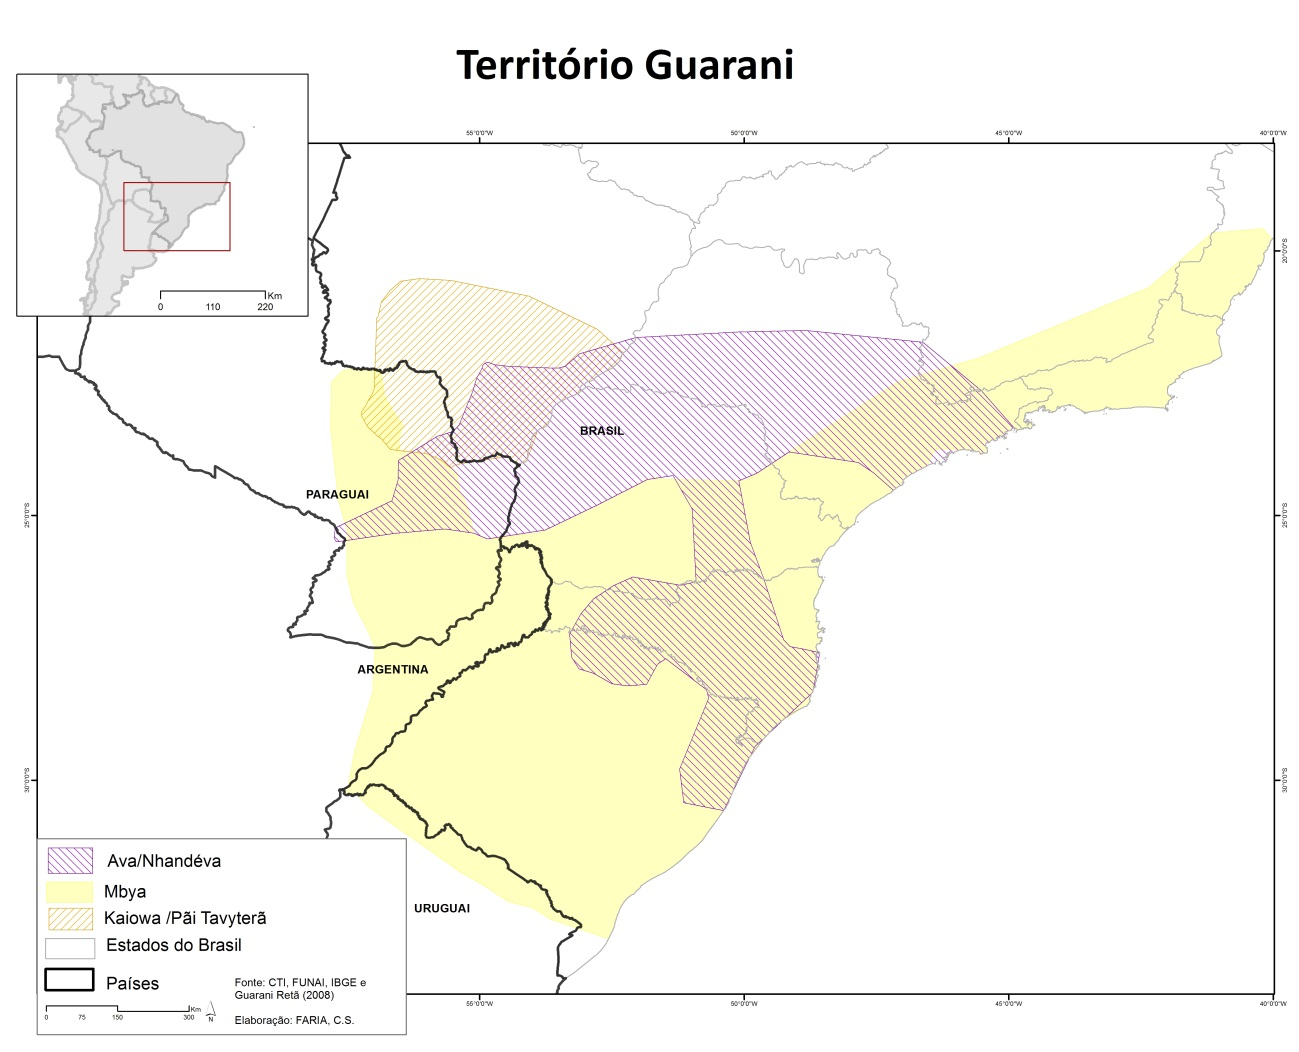
\includegraphics[width=5.8075in,height=4.528in]{livroredesguaranifinal-img7.jpg}
 

Mapa \stepcounter{Mapa}{\theMapa} -- Distribui\c{c}\~ao territorial
atual das parcialidades Guarani. Elabora\c{c}\~ao: Camila Salles de
Faria.

Durante meu trabalho de campo na TI Mbigua\c{c}u/SC, certo dia cheguei a
casa do casal de anci\~aos, onde encontrei Alcindo confeccionando um
pequeno balaio que lhe havia sido encomendado por uma vizinha. Na
ocasi\~ao, ele fez quest\~ao de destacar que aquilo n\~ao se tratava de
um ajaka, como se chamam as cestarias mbya, mas que era um mbajo, o
cesto antigo dos Chiripa, fabricado com cip\'o. Chamou-me a
aten\c{c}\~ao o destaque dado a tal diferencia\c{c}\~ao na cestaria,
por ela tamb\'em ter sido utilizada, nos anos 1930, pelo padre Franz
M\"uller (1989) como exemplo de diferen\c{c}as lingu\'isticas,
ideol\'ogicas e simb\'olicas entre os tr\^es agrupamentos Guarani
presentes na regi\~ao do Alto Paran\'a, que ficaram conhecidos pelas
designa\c{c}\~oes Mbya, Nhand\'eva (ou Chiripa) e Kaiowa. A
presen\c{c}a dessa grande diversidade na popula\c{c}\~ao guarani j\'a
havia sido apontada naquela regi\~ao por Nimuendaju (1914) alguns anos
antes.

Um investimento importante na caracteriza\c{c}\~ao das parcialidades
Guarani na etnografia s\~ao os diversos estudos feitos por Le\'on
Cadogan (1997; 1960; 1971), que a partir dos anos 1950 trouxeram \`a
luz diversas especificidades dos grupos Mbya no Paraguai, al\'em de
apontamentos comparativos com os Ava-Chiripa (1959) no Alto Paran\'a.
Menciono ainda duas refer\^encias que considero pontos-chave sobre o
delineamento das especificidades dos grupos Guarani no Paraguai, que
nos anos 1970 ampliam os apontamentos feitos por Cadogan, quais sejam
as etnografias de Miguel Bartolom\'e (1977), sobre os Av\'a-Katu-Ete, e
de Bartomeu Meli\`a, George \& Friedl Gr\"unberg (1976), sobre os
Pa\'i-Tavyter\~a. Em linhas gerais, estes estudos v\~ao caracterizar as
parcialidades como sendo os Pa$\text{\textgreek{~i}}$/Kaiow\'a um grupo
descendentes da redu\c{c}\~ao Itatim, com influ\^encia mais expl\'icita
do missionamento jesu\'itico; os Ava-Chiripa como grupos derivados da
redu\c{c}\~ao de Tarum\~a, com rela\c{c}\~oes mais intensas com os
colonos; e os Mbya como um agrupamento mais herm\'etico, que pode
manter-se mais afastado dos n\~ao-ind\'igenas. 

A obra de f\^olego de Egon Schaden (1962), em seus
{\textquotedblleft}aspectos fundamentais da cultura
guarani{\textquotedblright}, delineia as especificidades das
parcialidades no Brasil, tornando-se refer\^encia para as pesquisas
posteriores que se dedicaram a compreender a din\^amica territorial dos
Guarani e das rela\c{c}\~oes entre as parcialidades. Apesar de sua
inovadora modernidade, parece-me que a obra de Schaden peca por seu
enfoque na {\textquotedblleft}acultura\c{c}\~ao{\textquotedblright}, o
que n\~ao ofusca a sua qualidade descritiva e anal\'itica dos grupos
visitados pelo autor. Para compreender as articula\c{c}\~oes entre as
parcialidades nos estados do sul do Brasil, o estudo se faz incipiente,
estando restrito \`as aldeias Palmeirinha, no Paran\'a, e Limeira, no
oeste de Santa Catarina. Mas tem o m\'erito de identificar, j\'a nos
anos 1940, a movimenta\c{c}\~ao de grupos Mbya pelo Rio Grande do Sul,
avan\c{c}ando pelo litoral catarinense em dire\c{c}\~ao \`a regi\~ao
sudeste do pa\'is. Os grupos tomados como refer\^encia por Schaden para
descri\c{c}\~ao dos Ava-Chiripa, aos quais ele chama de Nhand\'eva, e
{\textquotedblleft}Mb\"ua{\textquotedblright}, s\~ao aqueles que \`a
\'epoca habitavam o estado de S\~ao Paulo, deixando um lapso com
rela\c{c}\~ao \`a sua presen\c{c}a na regi\~ao sul.

A presen\c{c}a dos coletivos Guarani no sul do Brasil passou a ser
objeto de estudos mais detalhados somente nos \'ultimos quinze anos e,
embora ainda care\c{c}a de uma s\'intese abrangente, estes trabalhos
permitem uma an\'alise dessas intrigantes articula\c{c}\~oes e
transforma\c{c}\~oes entre os grupos no n\'ivel regional. 

Inicio a reflex\~ao a partir da disserta\c{c}\~ao de Ivori Garlet
(1997), que mapeia a mobilidade de grupos Guarani no Rio Grande do Sul,
aos quais ele chama Mbya, trazendo uma importante reflex\~ao sobre a
continuidade entre estes e aqueles que se encontravam nas selvas do
Alto Paran\'a (Paraguai) e Missiones (Argentina) no fim da Guerra do
Paraguai, em 1870. Podemos considerar que estudos como os de Celeste
Ciccarone (2001), Maria In\^es Ladeira (2007; 2008), Jos\'e Basini
Rodrigues (1999), Aldo Litaiff (1996 e 1999) e Katia Vietta (1992),
entre outros, s\~ao pioneiros em descrever com maior detalhamento
diversos aspectos instigantes desta mobilidade mbya pelo interior do
Rio Grande do Sul, bem como seu avan\c{c}o pelo litoral atl\^antico
at\'e a regi\~ao sudeste do pa\'is e sua articula\c{c}\~ao com outros
grupos que j\'a se encontravam naquela regi\~ao. Entretanto, fa\c{c}o a
ressalva de que, com algumas exce\c{c}\~oes, tais estudos pecam em
n\~ao reconhecer apropriadamente a sobreposi\c{c}\~ao e a
co-habita\c{c}\~ao entre tais grupos mbya com os Chiripa, que
possu\'iam articula\c{c}\~oes relativamente estreitas, possivelmente
anteriores a esta movimenta\c{c}\~ao territorial.

Os primeiros estudos de f\^olego que tentam abarcar estas
articula\c{c}\~oes e transforma\c{c}\~oes entre as parcialidades Mbya e
Chiripa no sul do Brasil s\~ao as etnografias escritas por Fl\'avia
Cristina de Mello (2001; 2006; 2007), que nos trazem um preciso
delineamento das rela\c{c}\~oes entre esses grupos no litoral
catarinense e no interior do Rio Grande do Sul. A autora demonstra como
estes grupos se organizaram entre si pela sobreposi\c{c}\~ao de sua
mobilidade e co-habita\c{c}\~ao, constituindo diversos tipos de
alian\c{c}as no decurso do processo hist\'orico. Entretanto, nesta
esteira podemos somar outros estudos que apontam para este conv\'ivio
entre as parcialidades, como a tese de Maria Dorothea Darella (2004), a
disserta\c{c}\~ao de Fl\'avio Gobbi (2008) e outros, entre os quais
incluo a minha pr\'opria disserta\c{c}\~ao de mestrado (Oliveira,
2011). 

Penso que tal lapso possa ter influenciado algumas outras etnografias
posteriores que acabam por reificar uma totalidade mbya homog\^enea,
sem dar conta de forma apropriada da diversidade desta
composi\c{c}\~ao. Podemos dizer que, devido a complexidade do tema,
este tem sido um assunto evitado em diversas etnografias \`as quais
tive acesso. Al\'em disso, podemos pensar que essa unifica\c{c}\~ao em
torno de uma identidade mbya \'e uma quest\~ao incorporada pelos
Guarani no sul do Brasil, o que possivelmente contribui em dificultar a
percep\c{c}\~ao de diferen\c{c}as sutis entre as parcialidades,
imiscu\'idas em rela\c{c}\~oes de alian\c{c}a a parentesco.

Chiripa, Pa$\text{\textgreek{~i}}$, Tambeope

Desde o in\'icio de meu trabalho de campo na TI Mbigua\c{c}u, SC, para
realiza\c{c}\~ao de minha disserta\c{c}\~ao de mestrado (Oliveira,
2011), chamava-me aten\c{c}\~ao o fato de meu casal interlocutor,
Alcindo Moreira e Rosa Mariani Cavalheiro, que em linhas gerais se
auto-identifica aos n\~ao-\'indios como mbya, apontar recorrentemente a
sua diferen\c{c}a a outros grupos Guarani por serem do
{\textquotedblleft}costume chiripa{\textquotedblright}. Tal assertiva
passou a fazer sentido a partir de sinais diacr\'iticos que apontava o
casal como marcadores de sua diferencia\c{c}\~ao, que a todo momento
faziam refer\^encia aos aldeamentos em que o casal de anci\~aos havia
vivido sua inf\^ancia, no estado do Paran\'a. Optei por sistematizar
quatro elementos os quais in\'umeras vezes ouvi serem referenciados
pelo casal como marcadores de diferencia\c{c}\~ao entre grupos Guarani
Chiripa (que ficaram mais conhecidos como Nhand\'eva),
Pa$\text{\textgreek{~i}}$ (que ficaram mais conhecidos como Kaiowa) e
Tambeope (que vieram a ser conhecidos como Mbya), quais sejam: a
const\^ancia nos assentamentos, a indument\'aria, os h\'abitos
alimentares e a l\'ingua. 

A const\^ancia nos assentamentos \'e um dos elementos apontados pelo
casal como diacr\'itico entre seus grupos Chiripa e
Pa$\text{\textgreek{~i}}$ em rela\c{c}\~ao aos Tambeope. Segundo
relatam, os primeiros reuniam grande n\'umero de fam\'ilias em seus
aldeamentos, estabelecendo-se por longos per\'iodos de tempo em um
mesmo lugar. Por vezes as aldeias Chiripa e Pa$\text{\textgreek{~i}}$
abrigavam temporariamente fam\'ilias tambeope errantes, que eram
acolhidas como m\~ao de obra em suas lavouras e na cria\c{c}\~ao de
animais. Por diversas vezes ouvi alus\~oes de que os demais grupos
{\textquotedblleft}educavam{\textquotedblright} os Tambeope sobre os
costumes da agricultura e a religi\~ao dos Guarani. Obviamente a
const\^ancia nos assentamentos est\'a imbricada a diversos outros
aspectos do modo de vida, como as atividades agr\'icolas e a sua
mobilidade no territ\'orio.

Outro elemento bastante evidente sobre a forma de se reconhecerem
mutuamente as parcialidades era a indument\'aria. As vestimentas eram
marcadores n\'itidos da diferen\c{c}a e da pr\'opria denomina\c{c}\~ao
das parcialidades, sendo fabricadas com fios de algod\~ao cru ou com
fibras de pyno (urtig\~ao). Neste sentido, os Chiripa usavam cal\c{c}as
compridas chamadas de chiripas; os Pa$\text{\textgreek{~i}}$ utilizavam
ponchos longos que cobriam todo o corpo; e os Tambeope vestiam somente
pequenas batas atadas na cintura, chamadas de tambeo, motivo pelo qual
foram por vezes denominados na bibliografia como bat\'icolas.

O terceiro elemento apontado como fator de diferencia\c{c}\~ao entre as
parcialidades Guarani era a alimenta\c{c}\~ao, notavelmente associada a
constru\c{c}\~ao do corpo para a atividade xam\^anica. Segundo os
relatos de Rosa e Alcindo, de forma geral os grupos Chiripa e
Pa$\text{\textgreek{~i}}$ praticavam restri\c{c}\~oes alimentares mais
r\'igidas. Os primeiros comiam somente r\~as, peixes e eventualmente
lagartos, animais de sangue frio, centrando sua dieta no consumo de
bebida fermentada de milho, o kau$\text{\textgreek{~i}}$; enquanto os
segundos criavam uru{\textquoteright}\~u (corvos), que eram a principal
fonte proteica, consumida junto aos produtos das ro\c{c}as e frutas
coletadas nas matas. As carnes de ca\c{c}a eram utilizadas sobretudo
para o tratamento de doen\c{c}as, com o uso da gordura de animais
silvestres na prepara\c{c}\~ao de rem\'edios. Sobre os h\'abitos
alimentares dos Tambeope, Alcindo e Rosa afirmam que estes ca\c{c}avam
prioritariamente com o uso de armadilhas, sem seguirem r\'igidas
prescri\c{c}\~oes alimentares. Chamam a aten\c{c}\~ao para o fato de
que os grupos Tambeope estavam em intensa mobilidade, viajando longos
meses em jornadas em dire\c{c}\~ao ao litoral atl\^antico. 

O quarto elemento que aponto, tamb\'em bastante not\'orio, \'e a
l\'ingua. Podemos dizer que os dialetos nhand\'eva e kaiowa s\~ao mais
pr\'oximos entre si, portanto melhor compreens\'iveis, do que o mbya. O
casal marca que tal fator aumentava a articula\c{c}\~ao entre os
Chiripa e os Pa$\text{\textgreek{~i}}$, ao passo em que os distanciava
dos Tambeope, com quem tinham maior dificuldade para conversar. Alcindo
e Rosa fazem men\c{c}\~ao aos dialetos nhand\'eva e kaiowa com sendo a
{\textquotedblleft}l\'ingua antiga{\textquotedblright}, chamando a
aten\c{c}\~ao o fato de atualmente terem adotado o dialeto mbya em sua
fala cotidiana. Esse \'e um aspecto importante para pensarmos as
transforma\c{c}\~oes ocorridas no grupo
Chiripa/Pa$\text{\textgreek{~i}}$ a partir de suas articula\c{c}\~oes
com os grupos Mbya ao longo de sua mobilidade no territ\'orio.

A configura\c{c}\~ao Mbya

Em suas narrativas, Alcindo e Rosa costumam usar como marco de sua
hist\'oria de vida o {\textquotedblleft}tempo em que n\~ao existia
jurua{\textquotedblright}, a mobilidade decorrente da invas\~ao de suas
terras por colonizadores alem\~aes e o processo de demarca\c{c}\~ao do
territ\'orio no litoral de Santa Catarina. Segundo conta o casal, sua
idade \'e medida de fato pela {\textquotedblleft}taquara
seca{\textquotedblright}, que diz respeito ao per\'iodo de
florescimento do takua ete{\textquoteright}i (taquara-mansa), que
acontece em m\'edia a cada 30 anos; como eles dizem que teriam
assistido tal fen\^omeno por tr\^es vezes, proponho considerarmos que
tais eventos tenham ocorrido a partir dos anos 1920.

A sua hist\'oria de vida tem in\'icio na regi\~ao compreendida entre os
rios Igua\c{c}u e Paran\'a, onde viviam em dois aldeamentos chamados
Pari e Piracanju, separados em um grupo familiar
Pa$\text{\textgreek{~i}}$ e outro Chiripa, que possu\'iam v\'arios
tipos de alian\c{c}as entre si. O casal marca com precis\~ao a
articula\c{c}\~ao entre os grupos familiares dessas duas aldeias, que
permaneceram por diversos anos em assentamento constante, em
rela\c{c}\~ao aos Tambeope, que eventualmente permaneciam por curtos
per\'iodos abrigados em seus aldeamentos. Estas aldeias se desfazem a
partir do loteamento das terras no interior do Paran\'a, quando o grupo
familiar inicia um processo de mobilidade no territ\'orio em busca de
espa\c{c}os onde pudessem se reassentar e consolidar novos tekoha. O
casal Rosa e Alcindo passa a viver em peregrina\c{c}\~ao junto de seus
pais, oferecendo m\~ao-de-obra em fazendas e circulando por diversas
cidades dos estados de Santa Catarina e Rio Grande do Sul. Neste
movimento, o casal participa da funda\c{c}\~ao de aldeamentos que
atualmente ainda se encontram consolidados nesses estados, como Mato
Preto, Ara\c{c}\'a{\textquoteright}i, Campo Molhado, Granja Vargas,
Cacique Doble, Estiva, Cantagalo, Morro dos Cavalos, Mbigua\c{c}u,
entre outros\footnote{ Cf. Vietta (1992); Garlet (1997); Gobbi (2008);
Mello (2001; 2006; 2007); Darella (2004); Tommasino (2001); Ladeira
(2007; 2008).}.

Existem cerca de trinta \'areas de coabita\c{c}\~ao entre grupos Mbya e
Chiripa no sul do Brasil, que somam aproximadamente 5.500 \'indios
(BRASIL/SESAI, 2013\footnote{ Dispon\'ivel em:
{\textless}http://portalsaude.saude.gov.br/index.php/o-ministerio/principal/leia-mais-o-ministerio/70-sesai/9518-siasi{\textgreater}.}).
As articula\c{c}\~oes entre esses grupos, ocorridas ao longo deste
processo de intensifica\c{c}\~ao da coabita\c{c}\~ao, promoveram al\'em
de la\c{c}os matrimoniais e alian\c{c}as pol\'iticas e econ\^omicas,
uma aproxima\c{c}\~ao em outros campos, como o religioso e
principalmente o lingu\'istico, com a total incorpora\c{c}\~ao do
dialeto mbya. Esta aproxima\c{c}\~ao entre as duas parcialidades, que
passaram a se identificar com a designa\c{c}\~ao Mbya, teve efeito
tanto em rela\c{c}\~oes internas, com o estabelecimento de la\c{c}os
matrimoniais e alian\c{c}as pol\'iticas e econ\^omicas, como na
rela\c{c}\~ao externa na negocia\c{c}\~ao por reconhecimento pelo
Estado brasileiro.

Os Nhand\'eva contempor\^aneos

O centro territorial dos Nhand\'eva \'e a regi\~ao do Alto Paran\'a,
onde estavam intensamente concentrados no final do s\'eculo XIX,
servindo de m\~ao de obra na log\'istica da erva-mate no Brasil e no
Paraguai. Com o avan\c{c}o dos colonos paulistas e sulistas sobre o
Paran\'a e o Mato Grosso do Sul, no come\c{c}o do s\'eculo XX, os
Nhand\'eva sofrem uma dr\'astica perda de territ\'orio e acabam por ser
subjugados ao servi\c{c}o bra\c{c}al nas fazendas ou removidos para as
Reservas Ind\'igenas no Mato Grosso do Sul, no interior de S\~ao Paulo
e do Paran\'a, ou ainda levados para o Paraguai. \'E neste per\'iodo
hist\'orico que acontecem os movimentos migrat\'orios registrados por
Nimuendaju (1987), marcando a etnologia Guarani ao discorrer sobre a
busca da {\textquotedblleft}Terra Sem Males{\textquotedblright}. Os
Nhand\'eva fizeram a migra\c{c}\~ao para o litoral por duas rotas
distintas, uma pelo interior do Rio Grande do Sul e outra pelo interior
do Paran\'a at\'e S\~ao Paulo, em parte delas estabelecendo
coabita\c{c}\~ao com grupos Mbya, que vinham da regi\~ao de Misiones,
Argentina, e do sul do Paraguai.

Como mencionado, os grupos Nhand\'eva que na transi\c{c}\~ao para o
s\'eculo XX migraram para o Rio Grande do Sul e Santa Catarina, bem
como para o interior de S\~ao Paulo, eram chamados pelos outros grupos
de Chiripa. Podemos delinear duas levas migrat\'orias distintas de
grupos Nhand\'eva para o litoral e o interior de S\~ao Paulo, uma no
come\c{c}o do s\'eculo XX, relatada por Nimuendaju (1987), e outra a
partir nos anos 1960, com a expropria\c{c}\~ao do territ\'orio no oeste
do Paran\'a, no Paraguai e no Mato Grosso do Sul. Atualmente existem
doze \'areas de coabita\c{c}\~ao entre fam\'ilias Nhand\'eva e Mbya que
somam um contingente de cerca de 3.500 pessoas.

Embora estas movimenta\c{c}\~oes territoriais sejam ininterruptas, com
idas e vindas constantes de grupos familiares, elas se situam em
momentos coloniais espec\'ificos, uma no in\'icio da titula\c{c}\~ao
das terras e a explora\c{c}\~ao da m\~ao-de-obra na madeira e na
erva-mate; outra no avan\c{c}o da ocupa\c{c}\~ao efetiva do
territ\'orio por colonos (Myskyw, 2002; Cardoso \& Westphalen, 1986;
Ribeiro, 2002; Conradi, 2007). Nos anos 1970, com o avan\c{c}o da
agricultura mecanizada e a constru\c{c}\~ao da usina de Itaipu,
diversos grupos Nhand\'eva do Alto Paran\'a rumaram ao estado de S\~ao
Paulo por fugas e migra\c{c}\~oes volunt\'arias, articulando-se com
grupos Mbya que faziam o mesmo percurso. A disserta\c{c}\~ao de Daniel
Pierri (2013) descreve alguns desses grupos na regi\~ao do Vale do
Ribeira, falantes do dialeto mbya.

Os grupos assentados em reservas mais antigas, como as RIs Ararib\'a e
Serra do Itatins, mantiveram-se resistentes \`a presen\c{c}a de grupos
Mbya, n\~ao incorporando costumes religiosos e tampouco o dialeto,
autoidentificando-se normalmente como Nhand\'eva. Alguns desses grupos
constitu\'iram novos etn\^onimos de diferencia\c{c}\~ao, recusando
tamb\'em o termo chiripa, considerado pejorativo, e passando a se
autoidentificarem com Tupi-Guarani. Desta forma, percebe-se que de fato
existe um contraste entre os Tupi-Guarani e Nhand\'eva de S\~ao Paulo
com os Chiripa do sul do Brasil.

Os Nhand\'eva no Mato Grosso do Sul estavam concentrados sobretudo na
bacia mais ao sul do estado, na divisa com o Paraguai, sendo recolhidos
compulsoriamente para as reservas para a instala\c{c}\~ao das grandes
fazendas na regi\~ao. Nas Reservas Ind\'igenas foram colocados em
conv\'ivio for\c{c}ado com grupos Kaiowa, estabelecendo rela\c{c}\~oes
de conflito e alian\c{c}a.  Este per\'iodo de
desterritorializa\c{c}\~ao dos Guarani no Mato Grosso do Sul \'e
chamado por eles de sarambi {}--- espalhamento ---, ao qual se referem
em portugu\^es como {\textquotedblleft}o tempo do
corre-corre{\textquotedblright}, um deslocamento desordenado em
fun\c{c}\~ao da viol\^encia da coloniza\c{c}\~ao. Ocupam atualmente
nove Terras Ind\'igenas, em sua maioria compartilhadas com outros
grupos, al\'em de mais de 20 acampamentos que aguardam provid\^encias
para regulariza\c{c}\~ao fundi\'aria, somando um contingente de mais de
20 mil \'indios (SESAI, 2013). De forma geral, autoidentificam-se
simplesmente como Guarani, como um diferenciador em rela\c{c}\~ao aos
Kaiowa, com quem mant\'em um estreito v\'inculo pol\'itico em
fun\c{c}\~ao da luta pela demarca\c{c}\~ao de terras (Pereira, 1999;
Pimentel, 2012), sendo praticamente nula qualquer presen\c{c}a Mbya
entre esses grupos.

H\'a ainda outro contraste importante nas transforma\c{c}\~oes nos
Nhand\'eva contempor\^aneos, que s\~ao aqueles que n\~ao empreenderam
grandes movimentos migrat\'orios em dire\c{c}\~ao ao atl\^antico, mas
permaneceram nas margens brasileira e paraguaia do Rio Paran\'a e na
bacia do Iguatemi e na Serra do Maracaju, no Mato Grosso do Sul. Os
Nhand\'eva paranaenses se autoidentificam como Ava-Guarani, mesmo
nomenclatura utilizada no Paraguai e historicamente atribu\'ida ao
grupo, sendo muito pr\'oximos os Guarani sul-mato-grossenses. O grupo
teve maior visibilidade nos anos 1970 e 1980 em fun\c{c}\~ao da
constru\c{c}\~ao da usina de Itaipu que, associada ao processo de
esbulho praticado pelos colonos, pode ter removido cerca de seis mil
\'indios, que ocupavam mais de 40 aldeias (Carvalho, 2013; Peralta,
1995; Guaska, 2012), no oeste do Paran\'a. Estes \'indios da Tr\'iplice
Fronteira trabalharam nos ciclos econ\^omicos da regi\~ao e
permaneceram sujeitos a diversos tipos de viol\^encia para
expropria\c{c}\~ao de suas terras. Atualmente, est\~ao organizados em
cerca de 20 aldeias, que somam aproximadamente tr\^es mil \'indios
(SESAI, 2013), sendo que somente tr\^es delas est\~ao regularizadas.

A Tr\'iplice Fronteira \'e uma zona de micromobilidade Guarani que por
sua posi\c{c}\~ao geogr\'afica proporciona a influ\^encia dos grupos
Mbya de Missiones, na Argentina, e de grupos Ava dos departamentos de
Alto Paran\'a e Canindeyu, no Paraguai; como bem demonstra a tese de
Evaldo Mendes da Silva (2007).  \'E importante pontuar ainda a
presen\c{c}a de pessoas Mbya e Kaiowa entre os Ava-Guarani \'e comum,
por\'em bastante discreta, uma vez que muitos Ava foram removidos para
as reservas Kaingang no interior do Paran\'a, como Mangueirinha, Rio
das Cobras e Marrecas, coabitando com grupos mbya, sendo que outros
foram deslocados para as reservas Kaiowa, como Dourados, Amambai e
Caarap\'o. Seus v\'inculos se estendem ainda \`as reservas Nhand\'eva
no Mato Grosso do Sul, como Porto Lindo, Pirajui, Sombrerito,
Jaguapir\'e, o que lhes permitiu articula\c{c}\~ao com o movimento
ind\'igena Aty Guasu. Al\'em disso, diversas fam\'ilias Ava-Guarani
migraram ainda nos anos 1960 e 1970 para \'areas mais distantes, como
S\~ao Paulo, Rio de Janeiro e o litoral do Paran\'a, em fun\c{c}\~ao da
constru\c{c}\~ao da usina de Itaipu. Desta forma, seus v\'inculos de
alian\c{c}a alcan\c{c}am ainda algumas aldeias pr\'oximas ao litoral,
com grupos que tem identifica\c{c}\~ao com a etnog\^enese do Povo Mbya,
aproximando-se de sua principal organiza\c{c}\~ao etnopol\'itica, a
Comiss\~ao Guarani Yvyrupa.

  [Warning: Image ignored] % Unhandled or unsupported graphics:
%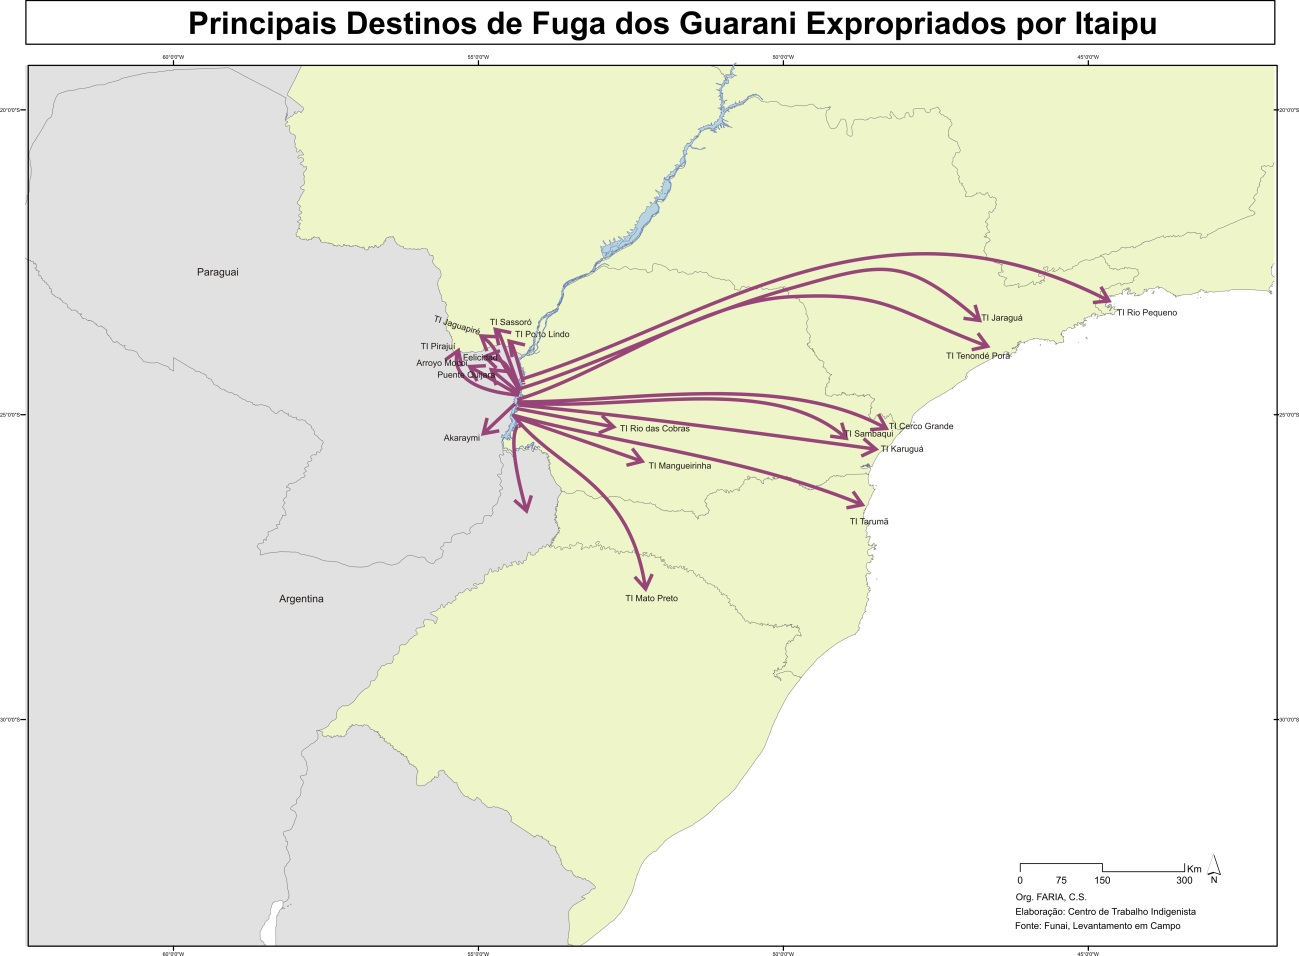
\includegraphics[width=5.9008in,height=4.1362in]{livroredesguaranifinal-img8.jpg}
 

Mapa \stepcounter{Mapa}{\theMapa} {}-- Rotas de migra\c{c}\~ao dos
Nhand\'eva a partir dos anos 1970. Elabora\c{c}\~ao: Camila Salles de
Faria.

Percebemos que a parcialidade tradicionalmente classificada como
Nhand\'eva comp\~oe atualmente uma gama de grupos ind\'igenas
brasileiros e transfronteiri\c{c}os, cujas especificidades est\~ao
associadas com as suas particularidades hist\'oricas. A etnologia
guarani ainda carece de uma obra de s\'intese abrangente sobre a
diversidade dos Nhand\'eva contempor\^aneos no Brasil, tratando-se de
um campo f\'ertil para estudos comparativos que deem conta da vasta
etnografia e sobretudo do necess\'ario trabalho de campo nessas
aldeias. Esta seria uma contribui\c{c}\~ao substancial para o
conhecimento sobre o povo Guarani em sua pluralidade atual. 

Refer\^encias

BARABAS, Alicia M. Los derechos ind\'igenas, la antropolog\'ia
jur\'idica y los movimientos etnopol\'iticos. Ilha 10(1), 2008.

BARBOSA, Pablo Antunha \& MURA, Fabio. Construindo e reconstruindo
territ\'orios Guarani: din\^amica territorial na fronteira entre Brasil
e Paraguai (sec. xix-xx). Journal de la soci\'et\'e des am\'ericanistes
97(2), 2011. 

BARTOLOM\'E, Miguel Alberto. Orekuera Royhendu (Lo que escuchamos en
sue\~nos): Shamanismo y religi\'on entre los Ava-Katu-Ete del Paraguay.
M\'exico: Instituto Indigenista Interamericano, 1977.

\_\_\_\_\_\_\_\_\_\_. Procesos interculturales: antropolog\'ia
pol\'itica del pluralismo cultural en Am\'erica Latina. M\'exico: Siglo
XXI Editores, 2006.

\_\_\_\_\_\_\_\_\_\_. Oguerojera (desplegarse). La etnogenesis del
pueblo mbya-guarani. Ilha 10(1), 2008.

BASINI RODRIGUES, Jos\'e E. Estrat\'egias econ\^omicas, pol\'iticas e
religiosas na mito-pr\'axis mby\'a-guarani. Disserta\c{c}\~ao de
Mestrado. Porto Alegre: UFRGS, 1999.

BRASIL. SESAI (Secretaria especial de Sa\'ude Ind\'igena). SIASI ---
Sistema de Informa\c{c}\~ao de Aten\c{c}\~ao \`a Sa\'ude Ind\'igena.
Bras\'ilia: Minist\'erio da Sa\'ude/SESAI, 2013.

BRIGHENTI, Cl\'ovis Ant\^onio.~Estrangeiros na pr\'opria
terra:~presen\c{c}a Guarani e Estados Nacionais.~Chapec\'o: ARGOS/Ed.
da UFSC, 2010. 

CADOGAN, Le\'on. Ayvu rapyta: textos m\'iticos de los Mby\'a-Guaran\'i
del Guair\'a. Asunci\'on: Ceaduc-Cepag, 1997 [1959].

\_\_\_\_\_\_\_\_\_\_. Como interpretan los Chirip\'a (Av\'a Guaran\'i)
la danza ritual. Revista de Antropologia 7(1-2), 1959.

\_\_\_\_\_\_\_\_\_\_. En torno de la aculturaci\'on de los
Mbya-Guaran\'i del Guair\'a. Am\'erica Ind\'igena XX(2), 1960. 

\_\_\_\_\_\_\_\_\_\_. Ywyra \~Ne{\textquoteright}ery: fluye del \'arbol
la palabra. Sugestiones para el estudio de la cultura guaran\'i.
Asunci\'on: CEPAG, 1971.

CARDOSO, Jayme; WESTPHALEN, Cec\'ilia. Atlas Hist\'orico do Paran\'a.
Curitiba: Livraria do Chaim, 1986.

CICCARONE, Celeste. Drama e sensibilidade. Migra\c{c}\~ao, xamanismo e
mulheres mbya guarani, Tese de Doutorado. S\~ao Paulo: PUC-SP, 2001.

CONRADI, Carla Cristina Nacke. As a\c{c}\~oes do Estado Nacional e a
trajet\'oria pol\'itica dos Guarani \~Nandeva no Oeste do Paran\'a
(1977-1997). Disserta\c{c}\~ao de Mestrado. Dourados: UFGD, 2007.

DARELLA, Maria Dorothea. Ore Roipota Yvy Por\~a, N\'os queremos terra
boa: territorializa\c{c}\~ao guarani no litoral de Santa Catarina,
Brasil. Tese de Doutorado. S\~ao Paulo: PUC-SP, 2004.

GARLET, Ivori Jos\'e.  Mobilidade mby\'a: hist\'oria e
significa\c{c}\~ao. Disserta\c{c}\~ao de Mestrado. Porto Alegre:
PUC-RS, 1997.

GOBBI, Fl\'avio S. Entre parentes, lugares e outros: tra\c{c}os na
sociocosmologia guarani no sul. Disserta\c{c}\~ao de Mestrado. Porto
Alegre: UFRGS, 2008.

GUASKA, Enrique. Del canto al llanto. Situaci\'on de las comunidades
ind\'igenas afectadas por la represa de Itaip\'u. Acci\'on 157, 2012.

LADEIRA, Maria In\^es Martins. O caminhar sob a luz. Territ\'orio mbya
\`a beira do oceano. S\~ao Paulo: Editora da UNESP, 2007.

\_\_\_\_\_\_\_\_\_\_. Espa\c{c}o geogr\'afico guarani-mbya: Significado,
constitui\c{c}\~ao e uso. S\~ao Paulo: Edusp, 2008.

LITAIFF, Aldo. As divinas palavras: identidade \'etnica dos
Guarani-Mby\'a. Florian\'opolis: Editora da UFSC, 1996.

\_\_\_\_\_\_\_\_\_\_. Les fils du soleil: mythes et pratiques d\^es
indiens mbya-guarani du littoral du Br\'esil. Tese de Doutorado.
Montr\'eal: Universit\'e de Montr\'eal, 1999.

MELI\`A, Bartolomeu; GR\"UNBERG, Friedl; GR\"UNBERG Georg. Los
Pai-Tavyter\~a. Etnograf\'ia guaran\'i del Paraguay contempor\'aneo.
Asunci\'on: Centro de Estudios Antropol\'ogicos de la Universidad
Cat\'olica, 1976.

MELI\`A, Bartomoleu. El Guarani conquistado y reducido: ensayos de
etnohistoria. Asunci\'on: Biblioteca Paraguaya de Antropolog\'ia, 1986.

{}---{}---{}---{}---{}---. A terra sem mal dos Guarani: economia e
profecia. Revista de Antropologia 33, 1990. 

{}---{}---{}---{}---{}---. El Guarani: experiencia religiosa.
Asunci\'on: Ceaduc-Cepag, 1991.

MELLO, Fl\'avia Cristina. Aata tap\'e rupy, seguindo pela estrada:~uma
investiga\c{c}\~ao dos deslocamentos territoriais de fam\'ilias
mby\'a-guarani no sul do Brasil.~Disserta\c{c}\~ao de Mestrado.
Florian\'opolis: UFSC, 2001.

{}---{}---{}---{}---{}---. Aetch\'a Nhanderukuery Karai Retar\~a. Entre
Deuses e Animais: Xamanismo, Parentesco e transforma\c{c}\~ao entre os
Chirip\'a e Mby\'a. Tese de Doutorado. Florian\'opolis: UFSC, 2006. 

{}---{}---{}---{}---{}---. Mby\'a e Chirip\'a: identidades \'etnicas,
etn\^onimos e autodenomina\c{c}\~oes entre os Guarani do sul do Brasil.
Tellus 7(12), 2007.

M\"ULLER, Pe. Franz. Etnografia de los Guarani del Alto Parana. Buenos
Aires: CAEA Ed., 1989.

MYSKIW, Antonio Marcos. Colonos, posseiros e grileiros: conflitos de
terras no Oeste Paranaense (1961/66). Disserta\c{c}\~ao de Mestrado.
Niter\'oi: UFF-UNIOESTE, 2002.

NIMUENDAJU, Curt.  As lendas de cria\c{c}\~ao e destrui\c{c}\~ao do
mundo como fundamentos da religi\~ao dos Apapoc\'uva-Guarani. S\~ao
Paulo: Hucitec/USP, 1987 [19l4].

OLIVEIRA, Diogo. Arandu Nhembo{\textquoteright}ea: Cosmologia,
Agricultura e Xamanismo entre os Guarani-Chirip\'a no litoral de Santa
Catarina. Disserta\c{c}\~ao de Mestrado. Florian\'opolis: UFSC, 2011.

PERALTA, Raquel. Los impactos de la Itaip\'u y las respuestas a los
mismos, de los Av\'a Chirip\'a, de acuerdo a su filosof\'ia sobre la
tierra. Monograf\'ia, 1995.

PEREIRA, Levi Marques. Parentesco e organiza\c{c}\~ao social kaiow\'a.
Disserta\c{c}\~ao de Mestrado. Campinas: UNICAMP, 1999.

PIMENTEL, Spensy K. Elementos para uma teoria pol\'itica kaiow\'a e
guarani.  Tese de Doutorado. S\~ao Paulo: PPGAS-USP, 2012.

RIBEIRO, Sara Iurkiv Gomes Tibes. O horizonte \'e a terra:
manipula\c{c}\~ao da identidade e constru\c{c}\~ao do ser entre os
guarani no Oeste do Paran\'a (1977-1997). Tese de Doutorado. Porto
Alegre: PUC-RS, 2002.

SCHADEN, Egon. Aspectos fundamentais da cultura guarani. S\~ao Paulu:
Difus\~ao Europeia do Livro, 1962.

SILVA, Evaldo Mendes da. Folhas ao vento: a micromobilidade de grupos
Mbya e Nhand\'eva (Guarani) na Tr\'iplice Fronteira. Tese de Doutorado.
Rio de Janeiro: PPGAS-Museu Nacional, 2007.

VIETTA, Katya. Mbya: guarani de verdade. Disserta\c{c}\~ao de Mestrado.
Porto Alegre: UFRGS, 1992.

Os pesquisadores que trabalham com os Guarani t\^em enfrentado
quest\~oes em que a bibliografia cl\'assica deixou uma lacuna, como do
que se fala quando se menciona coletivos, e do que se fala quando se
menciona redes. O culturalismo que guiou o trabalho de mission\'arios e
etn\'ologos na virada do s\'eculo XIX para o XX buscava recuperar a
diversidade na cultura material e em outros aspectos para a
constru\c{c}\~ao das etnias, como se fossem totalidades fechadas. Mas
se pode reconhecer na documenta\c{c}\~ao hist\'orica desde o s\'eculo
XVII a organiza\c{c}\~ao em redes. O crit\'erio de totalidades
\'etnicas como constru\c{c}\~ao da diferen\c{c}a aparece como
resultante do contato com os agentes coloniais. -- Marta Amoroso

Um nome que faz diferen\c{c}a: reflex\~oes com fam\'ilias tupi guarani.

L\'igia R. Almeida\footnote{* Doutora em antropologia social pelo
PPGAS-USP.}, Amanda C. Danaga\footnote{** Doutora em antropologia
social pelo PPGAS-UFSCar.}, Camila Mainardi\footnote{*** Doutora em
antropologia social pelo PPGAS-USP.}

Existem fam\'ilias tupi guarani em diferentes locais no estado de S\~ao
Paulo: no litoral e sudoeste do estado, em \'areas demarcadas ou n\~ao
e, ainda, em bairros de cidades como Mongagu\'a e Itanha\'em.\footnote{
Segundo o site da Comiss\~ao Pr\'o-\'indio de S\~ao Paulo, as TI
habitadas pelos Tupi Guarani e seus munic\'ipios s\~ao: Ararib\'a
(Ava\'i); Bananal (Peru\'ibe); Guarani do Aguape\'u (Mongagu\'a); Serra
de Itatins (Itariri); Jaragu\'a (S\~ao Paulo); Ribeir\~ao Silveira
(S\~ao Sebasti\~ao); Itaoca (Mongagu\'a); Pia\c{c}aguera (Peru\'ibe);
Renascer (Ubatuba); Bar\~ao de Antonina (Bar\~ao de Antonina); Guarani
de Itaporanga (Itaporanga) Tekoa Jaikoaty (Miracatu); Paranapu\~a
(S\~ao Vicente); Aldeinha (Itanhaem); Para\'iso (Iguape).Em algumas
dessas aldeias h\'a co-resid\^encia entre os Tupi Guarani, Guarani Mbya
e Terena. (Fonte: / http://www.cpisp.org.br/indios/html/uf.aspx?ID=SP,
informa\c{c}\~oes de 2012).} Neste texto privilegiamos as
experi\^encias de campo em tr\^es contextos etnogr\'aficos: aldeia Yvy
Pyha\'u, aldeia Ywyty Gua\c{c}u (ou aldeia Renascer) e nas aldeias da
TI Pia\c{c}aguera, localizadas respectivamente nos munic\'ipios de
Bar\~ao Antonina (sudoeste do estado de S\~ao Paulo), Ubatuba (litoral
norte do estado de S\~ao Paulo) e Peru\'ibe (litoral sul do mesmo
estado). Veremos que a no\c{c}\~ao de mistura\footnote{ Falas e
conceitos de nossos interlocutores tupi guarani ser\~ao grafados em
it\'alico no corpo do texto.}, evidenciada pelos usos e exegeses sobre
a autodenomina\c{c}\~ao Tupi Guarani, perpassa os tr\^es contextos,
relacionando-se com iniciativas de valoriza\c{c}\~ao cultural e de
retomada de terras tradicionais. A autodesigna\c{c}\~ao Tupi Guarani
expressa a mistura que segundo nossos interlocutores \'e resultante de
uma hist\'oria comum de intercasamentos entre diferentes povos,
ind\'igenas e n\~ao ind\'igenas. 

O uso de termos e categorias classificat\'orias se apresenta como algo
problem\'atico, na medida em que pode reificar fronteiras \'etnicas e
essencializar a configura\c{c}\~ao de grupos, ao ocultar as din\^amicas
relacionais entre eles e sua constante atualiza\c{c}\~ao. As
denomina\c{c}\~oes \'etnicas fazem parte dessas din\^amicas relacionais
que inventariam as alian\c{c}as que os grupos mant\^em com os outros,
sejam eles \'indios ou n\~ao \'indios, de maneiras muito diversas.
Sendo as rela\c{c}\~oes entre estes atores contextuais e baseadas em
diferentes experi\^encias, h\'a a necessidade de apreender os contextos
de enuncia\c{c}\~ao das denomina\c{c}\~oes \'etnicas. As fam\'ilias com
quem fizemos pesquisa compartilham a autodenomina\c{c}\~ao Tupi
Guarani, embora possam ser identificados por outras, como por exemplo,
a designa\c{c}\~ao Guarani Nhandeva.

Em raz\~ao de especificidades hist\'oricas, lingu\'isticas e culturais,
uma divis\~ao em subgrupos foi estabelecida por Egon Schaden (1954)
constituindo os Nhandeva, Mbya e Kaiow\'a.

Pesquisas de Ladeira e Azanha (1987) j\'a mencionavam o uso da
autodenomina\c{c}\~ao Tupi Guarani por algumas fam\'ilias do litoral
paulista, as quais tamb\'em s\~ao chamadas pelos Guarani Mbya de
Xirip\'a. Tal designa\c{c}\~ao \'e vista como pejorativa pelos Tupi
Guarani. Schaden (1954), a despeito de ter nomeado um subgrupo como
Nhandeva, reconhece essa express\~ao como a autodenomina\c{c}\~ao de
todos os Guarani, significando os que s\~ao dos nossos.

A respeito da defini\c{c}\~ao desse termo, Nimuendaju (1987: 7)
comentou: {\textquotedblleft}Os Guarani, ao falarem de si na sua
l\'ingua, para designar na\c{c}\~ao ou horda, empregam o termo
\~Nandeva, quando a pessoa com quem se fala pertence ao grupo, e
Or\'eva, quando pertence a uma outra tribo{\textquotedblright}.

Nos tr\^es contextos etnogr\'aficos abordados aqui, percebemos o uso do
termo nhandeva para se referirem aos parentes e a outros \'indios.
Fazem uso de nhandeva n\~ao como um etn\^onimo, uma categoria fixa que
remeteria a uma etnia, mas como forma de identificar-se enquanto
\'indios. Empregam o termo, em especial, em oposi\c{c}\~ao aos n\~ao
\'indios.\footnote{ No caso da Ywyty Gua\c{c}u, o termo \'e bastante
acionado para identificar uma oposi\c{c}\~ao em rela\c{c}\~ao \`as
fam\'ilias guarani mbya, com quem mant\^em co-resid\^encia.} O que
implica considerar Nhandeva como uma no\c{c}\~ao relacional, sujeita
aos contextos e aos atores em jogo.

As denomina\c{c}\~oes \'etnicas s\~ao, em geral, constru\'idas na
interface com os n\~ao \'indios, na rela\c{c}\~ao com o Estado --- mas
n\~ao s\'o --- e s\~ao imputadas de maneira arbitr\'aria, como no caso
da etn\^onimo Nhandeva. Para o caso das fam\'ilias tupi guarani,
apontamos que estas n\~ao aceitaram um nome imposto pelos n\~ao
\'indios, mas trataram de lhes ensinar que s\~ao Tupi Guarani. A
autodesigna\c{c}\~ao expressa a mistura, os casamentos entre Tupi e
Guarani, e tamb\'em com outros \'indios e n\~ao \'indios como
constituintes da pessoa Tupi Guarani, sendo aquilo que a singulariza e
n\~ao o que a descaracteriza, como pensam alguns.

Apesar de compartilharem o uso da autodenomina\c{c}\~ao Tupi Guarani, os
contextos que abordamos aqui possuem especificidades e autonomia. Neste
texto temos como objetivo mostrar que ser Tupi Guarani inclui uma
diversidade de possibilidades e que, no limite, uma aldeia pode trazer
\`a tona quest\~oes sobre as outras. Assim, apostamos que o conjunto
diverso de experi\^encias vivenciadas em campo\footnote{ Importante
pontuar que as autoras do texto n\~ao realizaram suas pesquisas de
campo conjuntamente. L\'igia R. de Almeida pesquisa juntos as
fam\'ilias tupi guarani da aldeia Ywy Pyha\'u, Amanda C. Danaga na
aldeia Renascer e Camila Mainardi, nas Terra Ind\'igena
Pia\c{c}aguera.} exprime aspectos do que \'e ser Tupi Guarani ---
condi\c{c}\~ao jamais dada, e sim constitu\'ida por rela\c{c}\~oes em
constante reconfigura\c{c}\~ao. Seguimos, ent\~ao, com os contextos
mencionados para tratar de quest\~oes que interessam aos nossos
interlocutores de modos e intensidades diferentes: a mistura e os
casamentos, as iniciativas de valoriza\c{c}\~ao cultural\footnote{
Cultura aqui em seu sentido aspeado, como sugere Manuela Carneiro da
Cunha para enfatizar o uso local que se faz da categoria cultura,
lembrando que {\textquotedblleft}a cultura de que falam os
antrop\'ologos n\~ao \'e a mesma da que falam os povos
ind\'igenas{\textquotedblright} e que cultura e
{\textquotedblleft}cultura{\textquotedblright} n\~ao pertencem ao mesmo
universo do discurso (2009: 313).}, as disputas territoriais e os
processos de demarca\c{c}\~ao da terra.  

Aldeia Ywy Pyha\'u: da luta pela terra ao fortalecimento da cultura

A aldeia Ywy Pyha\'u est\'a localizada no munic\'ipio de Bar\~ao de
Antonina, sudoeste do estado de S\~ao Paulo. At\'e o ano de 2014 era
formada por cinco fam\'ilias, somando um total de 30 pessoas.\footnote{
Vale lembrar que esses n\'umeros s\~ao vari\'aveis, pois dependem da
chegada e partida de pessoas e fam\'ilias.} A terra onde est\'a
localizada passa atualmente por um processo de regulariza\c{c}\~ao
fundi\'aria que se iniciou no ano de 2007, a partir de uma palestra
ministrada na Universidade Estadual Paulista (UNESP) de Araraquara pelo
ent\~ao cacique Marc\'ilio Marcolino.\footnote{ Esta Mesa Redonda foi
idealizada pelo Centro de Estudos Miguel \'Angel Men\'endez (CEIMAM) no
evento Amer\'india, que ocorreu em 2007.} Junto a antrop\'ologos e
membros do Minist\'erio P\'ublico, o cacique discursou sobre a
import\^ancia da terra para sua fam\'ilia Tupi Guarani, fazendo
cr\'iticas ferrenhas ao tratamento conferido aos povos ind\'igenas no
estado de S\~ao Paulo, baseado em paradigmas aculturativos e de perda
cultural. Em suas palavras, nos tratam como povos extintos. O mesmo
problema foi apontado em outro contexto por D. Juraci, a pessoa mais
velha da aldeia Ywy Pyha\'u:

Mas como n\'os desaparecemos se n\'os estamos aqui, nossa l\'ingua
est\'a aqui, nossa cultura est\'a aqui? N\'os falamos no verdadeiro
Tupi antigo, n\'os sempre fomos Tupi Guarani, o branco que quis mudar
isso. (Aldeia Ywy Pyha\'u, junho, 2010).

Dessa palestra surgiu uma carta reivindicando a constitui\c{c}\~ao de um
grupo t\'ecnico para realiza\c{c}\~ao dos estudos da terra. Na mesma
ocasi\~ao, Marc\'ilio fez quest\~ao de enfatizar que al\'em de terra
era preciso garantir o direito de sua fam\'ilia viver na cultura, de
ser Tupi Guarani. E foi assim, junto \`as reivindica\c{c}\~oes pela
terra e \`a busca de garantia de que poderiam, tal qual os
antigos\footnote{ Viver como os antigos, segundo moradores de Ywy
Pyha\'u, pressup\~oe uma terra boa, isto \'e, com mata, ca\c{c}a e
rios. Tamb\'em uma alimenta\c{c}\~ao composta menos de produtos
industrializados e mais de seus pr\'oprios cultivos, contando com milho
e mandioca para acompanhar a carne assada. Pressup\~oe ainda que tenham
for\c{c}a (mbaret\'e) e concentra\c{c}\~ao suficientes para dan\c{c}ar
e cantar, tornando-se leves para subir para Nhanderu  e ouvir o que ele
tem a lhes contar. O cuidado entre parentes \'e enfatizado como
fundamental para a aquisi\c{c}\~ao de tais qualidades.}, viver em uma
terra boa e pr\'oximos a Nhanderu, que iniciaram, em 2010, um movimento
pelo reconhecimento enquanto um grupo ind\'igena diferenciado.
Diferen\c{c}a esta marcada pela autodenomina\c{c}\~ao Tupi Guarani,
visto que eram conhecidos at\'e ent\~ao como Guarani Nhandeva. Segundo
D. Juraci, quando os n\~ao \'indios encontraram os Tupi Guarani e os
ouviram chamarem-se entre si de nhandeva, que traduzem como todos n\'os
\'indios, os denominaram dessa maneira, o que resultou na cren\c{c}a de
que os Tupi haviam desaparecido. {\textquotedblleft}Mas agora temos
voz, agora vamos falar, n\'os Tupi Guarani estamos aqui e vamos
fortalecer nossa cultura!{\textquotedblright} (Marc\'ilio Marcolino,
Aldeia Ywy Pyha\'u, 2010).

As fam\'ilias tupi guarani de Ywy Pyha\'u afirmam que s\~ao \'indios
misturados, em raz\~ao dos casamentos realizados entre os Tupinamb\'a e
Tupiniquim da costa litor\^anea e povos Guarani oriundos do Paraguai.
Mas a mistura e os casamentos que nela resultam, como apontado
anteriormente, remetem ainda aos casamentos com outros povos
ind\'igenas e com os n\~ao \'indios. Esses, em sua maioria, v\~ao morar
na aldeia e vivem mesmo como \'indio.

N\'os somos misturados, n\'os somos parentes dos Tupi que moravam no
litoral, em Santos, e que casaram aqui no meio do caminho com os
Guarani do Paraguai. Tem tamb\'em Xet\'a, Xokleng, Kaingang, mas tudo
\'indio puro, mas os principais mesmo foram esses dois (Marc\'ilio
Marcolino, aldeia Ywy Pyha\'u, 2010).

A mistura \'e fundamental na constitui\c{c}\~ao da pessoa e das
fam\'ilias Tupi Guarani e \'e constantemente acionada por essas
fam\'ilias de Ywy Pyha\'u para explicar o que consideram ser Tupi
Guarani. Entretanto, ela n\~ao \'e contr\'aria ao que consideram ser um
\'indio puro, aquele que fala a l\'ingua e vive segundo os costumes
ensinados por Nhanderu. Ser \'indio puro inclui ser \'indio misturado,
mas exclui a categoria mesti\c{c}o que, para essas fam\'ilias,
pressup\~oem a n\~ao viv\^encia na cultura.

Viver na cultura consiste em respeitar o que lhes ensina Nhanderu, bem
como o que lhes ensinam os mais velhos. \'E falar a l\'ingua ou
respeit\'a-la, alimentar-se com o que cultivam, ficar junto aos
parentes, cuidando e sendo cuidado. No entanto, no contexto atual em
que a terra que possibilita a viv\^encia como no tempo dos antigos se
torna escassa e que o respeito aos povos e direitos ind\'igenas vem
sendo amea\c{c}ados, \'e preciso ainda que constituam alian\c{c}as com
parceiros variados, em busca do que denominam fortalecimento cultural. 


O \'indio s\'o \'e respeitado como \'indio quando usa um cocar. Se
est\'a vestido como um branco, as pessoas acham que deixou de ser
\'indio. Precisamos sempre mostrar nossa cultura! (Marc\'ilio
Marcolino, Aldeia Ywy Pyh\'au, 2010).

Como forma de mostrar a cultura tupi guarani, as fam\'ilias de Ywy
Pyha\'u planejam fazer um almanaque contando sua hist\'oria. Buscam,
tamb\'em, espa\c{c}o para o ensino da l\'ingua, incluindo nas apostilas
ind\'igenas o ensino do tupi antigo, pois ressentem da predomin\^ancia
da l\'ingua Guarani nos materiais did\'aticos.\footnote{ Relatam que,
nos materiais did\'aticos enviados \`a escola, a l\'ingua Guarani ou
Mbya tem mais espa\c{c}o do que o Tupi Guarani (tupi antigo). As
crian\c{c}as aprendem a l\'ingua nas {\textquotedblleft}aulas de
cultura{\textquotedblright} ministradas na escola da aldeia e tamb\'em
no conv\'ivio di\'ario com seus parentes, sobretudo, com D. Juraci.}
Al\'em de projetos que visam o ensino da l\'ingua, outra forma
encontrada de divulgar seu universo cultural e os projetos de Ywy
Pyha\'u foi a grava\c{c}\~ao aut\^onoma de um DVD, em que se pode
conhecer um pouco mais sobre essas fam\'ilias e sua aldeia. O
financiamento para a confec\c{c}\~ao deste DVD foi captado atrav\'es do
envio de projetos ao ProAC, concurso promovido pela Secretaria de
Cultura do Estado de S\~ao Paulo. O intuito do ProAC \'e oferecer a
essas comunidades apoio cultural aos projetos que visam o
fortalecimento das culturas ind\'igenas. 

Tais iniciativas demonstram a import\^ancia da constitui\c{c}\~ao de
alian\c{c}as com parceiros outros, \'indios de aldeias pr\'oximas e
n\~ao \'indios engajados na elabora\c{c}\~ao e execu\c{c}\~ao de
projetos culturais que visam a conquista e manuten\c{c}\~ao de
direitos. O fortalecimento cultural dessas fam\'ilias, atrav\'es da
demarca\c{c}\~ao de sua terra e dos projetos mencionados s\~ao uma
forma de continuar existindo, como costuma enfatizar o cacique
Marc\'ilio Marcolino.  

Iniciativas de valoriza\c{c}\~ao cultural na TI Pia\c{c}aguera

A TI Pia\c{c}aguera est\'a localizada no munic\'ipio de Peru\'ibe,
litoral sul do estado de S\~ao Paulo. Ao final de 2014, possu\'ia cinco
aldeias --- Pia\c{c}aguera, Nhamandu Mirim, Taba\c{c}u Rekoypy,
Tanygu\'a e Kuara{\textquoteright}y-Mirim --- n\'umero variante tanto
porque a reconfigura\c{c}\~ao de aldeias \'e constante, como porque o
estabelecimento e manuten\c{c}\~ao destas depende do prest\'igio de uma
lideran\c{c}a em manter os parentes reunidos, al\'em da
legitima\c{c}\~ao dos demais parentes e de n\~ao ind\'igenas. Um novo
coletivo vai se conformando na medida em que \'e reconhecido e nomeado
pelos demais parentes ({\textquotedblleft}aldeia X{\textquotedblright}
ou {\textquotedblleft}aldeia de fulano{\textquotedblright}) em
coment\'arios como: Agora aqui [na TI] tem cinco aldeias!, ou em outros
que questionam a nova configura\c{c}\~ao: Como podem se considerar uma
aldeia?. Trata-se de um processo que n\~ao se conclui --- j\'a que o
esfor\c{c}o em fazer ou refazer coletivo \'e constante --- e do qual
participam atores n\~ao ind\'igenas, tanto colaboradores em projetos e
pol\'iticas -- que podem possibilitar a abertura de salas de aula, o
atendimento m\'edico, atividades de valoriza\c{c}\~ao cultural --- como
n\~ao ind\'igenas contr\'arios ao estabelecimento de novos coletivos,
em especial em casos de forma\c{c}\~ao de aldeias em \'areas n\~ao
demarcadas. 

Em Pia\c{c}aguera, TI homologada no ano de 2011 (FUNAI: BSB/305/02),
iniciativas de promo\c{c}\~ao cultural s\~ao um modo de se relacionar
com alguns n\~ao ind\'igenas, assim como mobilizam rela\c{c}\~oes entre
pessoas e fam\'ilias na TI. Iniciativa comum nas aldeias s\~ao as
apresenta\c{c}\~oes de grupos musicais\footnote{ Vale lembrar, contudo,
que os integrantes dos grupos musicais variam. A pr\'opria
manuten\c{c}\~ao do grupo e maior ou menor atua\c{c}\~ao deste depende
do prest\'igio de quem o encabe\c{c}a, na maioria dos casos o cacique.
O mesmo ocorre com as iniciativas de receber turistas nas aldeias que
dependem do apoio e participa\c{c}\~ao dos parentes.}, al\'em da
recep\c{c}\~ao de turistas para viv\^encias e palestras. A aldeia
Nhamandu Mirim, por exemplo, tem um blog com fotos, not\'icias sobre a
demarca\c{c}\~ao territorial e a seguinte mensagem do cacique:

A todos que apreciam a cultura ind\'igena primeiramente sejam bem vindo
ao nosso blog, em segundo meu nome \'e Cacique Domingos, sou
respons\'avel pela aldeia Nhamand\'u Mirim, estamos em constante
mudan\c{c}as para interagir com a popula\c{c}\~ao e ensinarmos a nossa
cultura, estamos expandindo nossos horizontes dentro da aldeia, para
viabilizar uma forma adequada de turismo ecol\'ogico, onde os
visitantes ter\~ao um dia de aprendizado sobre a arte de viver na mata,
caminhando por trilhas, assistindo a cantos e dan\c{c}as e pe\c{c}as de
teatros sobre a nossa cultura, vivendo da ca\c{c}a e da pesca e dos
artesanatos, esperamos muito em breve estar recebendo um grande
n\'umero de visitantes que tem o desejo de entender como vivemos em
harmonia com a natureza, para maiores informa\c{c}\~oes entre em
contato pelo telefone celular [n\'umero] (Cacique Domingos, aldeia
Nhamandu Mirim).

A mensagem do cacique Domingos, assim como as apresenta\c{c}\~oes para
n\~ao ind\'igenas dentro e fora das aldeias que comp\~oem a TI, s\~ao
justificadas pela necessidade de ensinar os brancos. No
v\'ideo-document\'ario produzido durante a grava\c{c}\~ao do CD
Kangwa\'a:  cantando para Nhanderu, Itamirim disse que muitas pessoas
pensam que o ind\'igena \'e incapaz, eles acham que o ind\'igena tem
que viver no mato pelado e n\~ao evolui. O pensamento mais ou menos
hegem\^onico entre os brancos, apontado por Itamirim, \'e o do atraso e
n\~ao desenvolvimento dos coletivos ind\'igenas.\footnote{ O que
tamb\'em aparece na fala do cacique Marc\'ilio da aldeia Pyha\'u, como
comentado no t\'opico anterior deste ensaio.} Pensamento equivocado,
sabemos, j\'a que a cultura n\~ao se constitui como unidade fixa, muito
menos deve ter como modelo de desenvolvimento os brancos. Para fazer
frente a esse pensamento, as fam\'ilias de Pia\c{c}aguera julgam
importante divulgar suas m\'usicas e se tornarem vis\'iveis em sua
diferen\c{c}a aos olhos dos brancos.

No v\'ideo-document\'ario mencionado, Catarina e Dora explicaram a
conforma\c{c}\~ao do etn\^omimo Tupi Guarani. Catarina disse: 

Eu sou Tupi Guarani porque meus pais por parte de m\~ae eram Tupi que
morava nessa regi\~ao, faziam parte dos Tupinamb\'a. E os Guarani
vieram do Mato Grosso do Sul e outros do Rio Grande do Sul. E a minha
fam\'ilia misturou o Tupi com o Guarani.

O mesmo foi reiterado por Dora: Meus pais eram ind\'igenas, minha m\~ae
Guarani Mbya e meu pai Tupinamb\'a, e a\'i se misturou e eu sou Tupi
Guarani.

Na \'epoca dos estudos complementares sobre a TI, que objetivava dar
continuidade ao processo de demarca\c{c}\~ao territorial, v\'arias
narrativas trataram da mesma quest\~ao. Citamos aqui a fala de
Am\^ancio, irm\~ao de Catarina:

N\'os somos Tupi Guarani... Mas, enfim, porque hoje os Tupi j\'a est\~ao
casados com Guarani tamb\'em. N\~ao s\'o com Guarani, mas com pessoas
brancas tamb\'em, tem j\'a v\'arias misturas, n\'os j\'a viemos de
mistura. (...) Ent\~ao, n\'os temos v\'arias misturas, n\'os temos o
Tupi, o Guarani, Kaingang, Kaiow\'a, at\'e a mistura de negros, porque
meu v\^o e minha v\'o, da parte do meu pai, eles eram negros. Mas,
assim, \'e \'indio. 

Nessas falas, a mistura \'e positivada em detrimento da ideia de pureza
--- e, portanto, de qualquer unidade com fronteiras definidas --- que,
em geral, est\'a vinculada aos etn\^onimos.\footnote{ Segundo Taylor
(1985) a unidade pressuposta pelo etn\^onimo mascara a
diferencia\c{c}\~ao explicitada por outros mecanismos. Apesar dos
esfor\c{c}os e problematiza\c{c}\~oes dos antrop\'ologos, em geral, nas
rela\c{c}\~oes com o Estado e pol\'iticas de valoriza\c{c}\~ao da
{\textquotedblleft}cultura{\textquotedblright}, cada povo ind\'igena
possui um nome, uma cultura, uma l\'ingua.  } As falas sobre a
conforma\c{c}\~ao \'etnica lan\c{c}am luz \`as preocupa\c{c}\~oes caras
\`as fam\'ilias Tupi Guarani na TI Pia\c{c}aguera: os casamentos e a
gera\c{c}\~ao de crian\c{c}as, destacando a mistura como din\^amica
inerente \`a constru\c{c}\~ao do parentesco.

Os casamentos est\~ao envoltos em intenso debate. No limite, tais
discuss\~oes t\^em em vista aqueles com quem desejam compartilhar o dia
a dia e aqueles {\textquotedblleft}indesejados{\textquotedblright}, o
que, em geral, independe de serem ind\'igenas ou brancos. O ponto \'e
que os casamentos s\~ao assuntos importantes e lan\c{c}am luz \`as
narrativas sobre a mistura e o etn\^onimo Tupi Guarani.

Vale lembrar que os brancos s\~ao m\'ultiplos. Alguns podem ser
ensinados a respeitar essa diferen\c{c}a nos projetos e eventos de
enuncia\c{c}\~ao cultural; outros podem ser tornados parentes por meio
de casamentos. Mas h\'a aqueles cuja aproxima\c{c}\~ao \'e indesejada
ou invi\'avel. H\'a n\~ao ind\'igenas que moram nos limites da TI cuja
rela\c{c}\~ao \'e de evita\c{c}\~ao\footnote{ H\'a casas de banhistas
com piscina e bonitos jardins, que ficam sob o cuidado de caseiros, mas
de quem dificilmente se ouve qualquer coment\'ario.}, por\'em com
outros compartilham festas, jogos de futebol e o trabalho fora das
aldeias -- nos quiosques da praia ou na constru\c{c}\~ao civil, por
exemplo. Com os \'ultimos o casamento \'e poss\'ivel. Morar junto (ou
perto), compartilhar o cotidiano, os eventos mencionados, as
refei\c{c}\~oes, colocam a possibilidade de casamentos, constr\'oi
parentesco. 

Entre outros: agenciamentos das rela\c{c}\~oes na aldeia Ywyty Gua\c{c}u


As rela\c{c}\~oes com outros (fam\'ilias guarani mbya e n\~ao \'indios)
s\~ao marcadas por proximidades e distanciamentos que perpassam a
trajet\'oria e o cotidiano das fam\'ilias tupi guarani que vivem na
aldeia Ywyty Gua\c{c}u (Morro Grande --- em refer\^encia ao Morro do
Corcovado que circunda a aldeia), tamb\'em conhecida como aldeia
Renascer. Tais rela\c{c}\~oes caracterizam a pr\'opria no\c{c}\~ao de
pessoa tupi guarani, calcada na ideia de mistura. Caracterizam,
inclusive, o processo de constitui\c{c}\~ao da aldeia, formada a partir
das grava\c{c}\~oes do longa-metragem do diretor Luis Alberto Pereira,
intitulado Hans Staden\footnote{ As grava\c{c}\~oes de Hans Staden
iniciaram-se em agosto de 1997. O lan\c{c}amento do filme ocorreu em
dezembro de 1999.}. O local onde hoje \'e a aldeia foi o cen\'ario
utilizado para a produ\c{c}\~ao do filme e alguns \'indios foram
convidados para participarem das grava\c{c}\~oes. Para a filmagem foram
feitas grandes ocas cenogr\'aficas semelhantes \`as moradias dos
antigos Tupinamb\'as que habitavam a costa litor\^anea brasileira em
meados do s\'eculo XVI. Ant\^onio da Silva Aw\'a, atual cacique da
aldeia, participou do filme em um curto papel figurativo. Com o
t\'ermino das grava\c{c}\~oes, a aldeia cenogr\'afica permaneceu
abandonada e as fam\'ilias tupi guarani passaram a frequentar as
grandes ocas. Sob a lideran\c{c}a de Aw\'a e sua afirma\c{c}\~ao de que
onde tem oca tem \'indio, essas fam\'ilias fixaram-se na \'area, dando
origem \`a aldeia.

O contexto no qual a Ywyty Gua\c{c}u se formou aponta para uma quest\~ao
interessante: o surgimento de uma aldeia real a partir de uma aldeia
cenogr\'afica e a influ\^encia do filme neste processo, visto que o
mesmo trabalhou com imagens que rememoravam a um poss\'ivel passado dos
Tupi Guarani.\footnote{ Conforme citado em momento anterior, os Tupi
Guarani afirmam sua origem como resultante de um processo de mistura
entre duas matrizes distintos, os Tupinamb\'a e os Guarani. Sendo que
os Tupi Guarani da aldeia Ywyty Gua\c{c}u n\~ao excluem os n\~ao
\'indios desse processo.} Contudo, o filme aparece como um fator
coadjuvante no processo de constitui\c{c}\~ao da \'area. Os moradores
da aldeia n\~ao deixam de mencion\'a-lo enquanto um elemento que
facilitou a aglutina\c{c}\~ao de algumas fam\'ilias. Segundo dizem, o
filme possibilitou o encontro entre as fam\'ilias para realiza\c{c}\~ao
de um desejo que lhes era comum: o engajamento com projetos de
preserva\c{c}\~ao da tradi\c{c}\~ao na reocupa\c{c}\~ao de
territ\'orios reconhecidos pelos ind\'igenas como tradicionais. Assim,
o filme foi apenas o cen\'ario que favoreceu a realiza\c{c}\~ao de suas
inten\c{c}\~oes, que estavam diretamente conectadas \`a rela\c{c}\~ao
que sua falecida m\~ae marcava com a regi\~ao de Ubatuba. \footnote{ Ao
assistirem uma c\'opia do filme n\~ao legendada --- a~l\'ingua~falada
pelos atores no filme \'e predominante o~tupi {}--- alguns adultos
\emph{comentaram sobre a linguagem usada e ressaltaram a diferen\c{c}a
entre a fala do filme e a fala deles:}\emph{ Parece que eles est\~ao
lendo... }As rea\c{c}\~oes mais c\^omicas, ao verem o filme, partiam
das crian\c{c}as, quando viam os atores nus, inclusive Aw\'a.}

Minha m\~ae tinha alguma coisa com esse lugar, ela nunca tinha vindo pra
c\'a, mas falava sempre daqui. Ela deve ter visto em sonho (...) O
sonho da minha m\~ae era essa regi\~ao, n\~ao aqui, a Ywyty Gua\c{c}u,
mas essa regi\~ao (...) Eu estou seguindo o caminho dela e ela vai
estar comigo, trabalhando junto (Antonio Aw\'a, Aldeia Renascer, 2009).

Segundo Aw\'a, sua m\~ae sempre comentava sobre a regi\~ao de Ubatuba,
local onde desejava residir um dia. Quando surgiu a oportunidade de
participar do filme foi que ele conheceu o lugar no qual fundaria a
Ywyty Gua\c{c}u. Houve uma grande identifica\c{c}\~ao entre o local
conhecido e o local apontado por sua m\~ae. Em virtude disso,
juntamente com outras fam\'ilias, Aw\'a optou por permanecer na \'area
habitando inicialmente a aldeia cenogr\'afica. Com o passar do tempo,
ap\'os instalarem-se nas ocas cenogr\'aficas, as fam\'ilias sa\'iram
delas e constru\'iram suas casas, mesmo porque as ocas utilizadas como
cen\'ario foram sucumbindo no transcorrer dos anos. 

Apesar do contexto caracter\'istico de forma\c{c}\~ao da aldeia n\~ao
definir uma rela\c{c}\~ao de causalidade~com o processo das filmagens,
o uso das c\^ameras e o registro de imagens na Ywyty Gua\c{c}u \'e
intenso. Durante a estadia do Grupo T\'ecnico\footnote{ Importante
ressaltar que o contexto deste campo em 2009 foi marcado pelo processo
de reivindica\c{c}\~ao e reconhecimento territorial, no qual um Grupo
T\'ecnico realizou o relat\'orio de fundamenta\c{c}\~ao antropol\'ogica
da \'area.} que realizava os estudos antropol\'ogicos da \'area, Aw\'a
procurava registrar todos os acontecimentos do trabalho, pois isso era
uma maneira de transmitir para as gera\c{c}\~oes futuras como aconteceu
o processo de defini\c{c}\~ao da \'area, al\'em de promover o
reconhecimento em diversos outros aspectos, por parte dos outros grupos
que vivem na regi\~ao e dos n\~ao \'indios. Se Aw\'a morre e n\~ao
passa nada? Se eu morro e meus filhos crescem sem passar sua cultura,
n\~ao \'e culpa deles, \'e culpa do velho, ele que n\~ao ensinou nada
aos jovens. 

O anseio pelo registro, produ\c{c}\~ao, veicula\c{c}\~ao e armazenamento
das imagens e v\'ideos que falavam sobre as hist\'orias da aldeia, era
constante.\footnote{ H\'a um arquivo de fotos e reportagens sobre a
aldeia, desde sua forma\c{c}\~ao at\'e os dias atuais, e um blog
dispon\'ivel na internet, que conta um pouco sobre a hist\'oria e o dia
a dia da aldeia, al\'em de uma p\'agina no Facebook. Para consultar o
blog, acesse:
{\textless}http://aldeiarenascer.blogspot.com{\textgreater}.} No
primeiro dia e no \'ultimo dia em que a equipe do GT esteve na aldeia,
a lideran\c{c}a pediu para que fosse feita uma fala que delineasse um
pouco sobre as expectativas e impress\~oes acerca do trabalho
desenvolvido, para que isso ficasse registrado em v\'ideo. O cuidado
com as imagens e com as grava\c{c}\~oes aparecia em v\'arias
ocasi\~oes, como, por exemplo, quando pediam para ligar ou desligar o
gravador de acordo com o que queriam dizer ou quando enfatizavam
quest\~ao da autoria das imagens ao disponibilizarem suas fotografias.

Por diversas vezes, inclusive em per\'iodos posteriores \`a pesquisa
para a regulariza\c{c}\~ao da terra, Aw\'a requisitava o registro das
reuni\~oes e dos encontros que aconteciam dentro e fora da TI. Em
algumas ocasi\~oes, requisitou a grava\c{c}\~ao das crian\c{c}as
cantando para que ele pudesse ouvir e analisar se estava bom e se elas
haviam evolu\'ido com os ensaios. Quando turistas chegavam a fim
conhecer a \'area, Aw\'a era sempre comunicado, caso contr\'ario, n\~ao
poderiam tirar fotos. Al\'em disso, as pessoas pediam as fotos tiradas
na aldeia, dizendo que gostariam de por em um quadro. Em todas as
casas, especificamente nas dos Tupi Guarani,\footnote{ Na Ywyty
Gua\c{c}u h\'a coexist\^encia de fam\'ilias tupi guarani e fam\'ilias
guarani mbya. As distin\c{c}\~oes entre essas fam\'ilias s\~ao
constantemente assinaladas nas rela\c{c}\~oes entre elas. } e na escola
h\'a muitas fotografias emolduradas.

Nos mais variados contextos, a invoca\c{c}\~ao de uma singularidade
cultural visa garantir direitos e reconhecimento em muitos aspectos,
como no caso da autodenomina\c{c}\~ao Tupi Guarani. Mas tamb\'em
mobiliza reflex\~oes do grupo sobre sua pr\'opria origem e
singularidade. Nesse sentido, a produ\c{c}\~ao/veicula\c{c}\~ao de
imagens sinaliza um di\'alogo com aqueles que vivem fora que \'e, ao
mesmo tempo, indissoci\'avel do di\'alogo entre aqueles que vivem
dentro da aldeia. Como salientou Marcela Coelho de Souza (2010), os
enunciados da cultura seriam {\textquotedblleft}efeitos do
encontro{\textquotedblright} com o n\~ao \'indio. \footnote{
{\textquotedblleft}Quando usam nossa palavra --- ou alguma
tradu\c{c}\~ao engenhosa dela --- eles est\~ao produzindo um objeto que
significa sua rela\c{c}\~ao conosco, mas trata-se ainda da
produ\c{c}\~ao deles: o que eles devem estar fazendo --- eles n\~ao tem
alternativa --- n\~ao \'e objetificar sua cultura (sem aspas) por meio
do nosso conceito, mas sua rela\c{c}\~ao conosco por meio dos conceitos
deles --- quero dizer, por meio de sua pr\'opria compreens\~ao do que
constitui criatividade, agencia, subjetividade{\textquotedblright}
(Coelho de Souza, 2010: 112).}

Por fim, produzir fotografias, registrar imagens, criar v\'ideos,
envolver-se em projetos e fazer festas s\~ao formas de dar visibilidade
\`a cultura acionadas pelas fam\'ilias da Ywyty Gua\c{c}u. Vale lembrar
que s\~ao m\'ultiplos os enunciados e as rela\c{c}\~oes por meios
culturais e que essa multiplicidade tamb\'em se reflete na
acep\c{c}\~ao da {\textquotedblleft}cultura{\textquotedblright} como
uma ferramenta de di\'alogo, ampliando suas possibilidades de
conex\~oes sociais e de sentido.

Ser Tupi Guarani \'e fugir de essencialismos

{\textquotedblleft}Qualquer essencialismo \'e
enganoso{\textquotedblright}, advertiu Carneiro da Cunha ao mostrar que
{\textquotedblleft}etnicidade{\textquotedblright}, entendida como
linguagem em que o repert\'orio cultural \'e acionado para produzir
distin\c{c}\~oes entre segmentos sociais, \'e antes um processo do que
algo fixo e estabilizado. Contudo, a autora assinala que a quest\~ao
ind\'igena sempre esteve permeada de reifica\c{c}\~oes. Entre
{\textquotedblleft}bons e maus selvagens do s\'eculo
XVI{\textquotedblright} at\'e {\textquotedblleft}ec\'ologos por
natureza e inimigos do progresso nos dias atuais{\textquotedblright},
as popula\c{c}\~oes ind\'igenas sempre tiveram de se ver frente aos
estere\'otipos que lhes s\~ao constru\'idos (Carneiro da Cunha, 2012:
120-4). No caso das fam\'ilias tupi guarani que vivem no estado de
S\~ao Paulo, elas n\~ao acolheram um nome imposto pelos n\~ao \'indios
--- tal como a classifica\c{c}\~ao Guarani Nhandeva --- e lutaram (e
ainda lutam) pela desconstru\c{c}\~ao de um estere\'otipo de
{\textquotedblleft}indianidade{\textquotedblright}, afirmando aos n\~ao
\'indios sua condi\c{c}\~ao Tupi Guarani, resultante de uma hist\'oria
comum de intercasamentos entre diferentes povos. 

Este texto buscou, por meio de diferentes contextos etnogr\'aficos,
apresentar as explica\c{c}\~oes sobre a conforma\c{c}\~ao do etn\^onimo
Tupi Guarani, que expressam a mistura, os casamentos entre fam\'ilias
Guarani e Tupi, mas de modo particular em cada contexto. Assim,
abordamos tamb\'em as rela\c{c}\~oes que constituem e s\~ao
constitu\'idas pelas fam\'ilias Tupi Guarani, em especial no que diz
respeito aos n\~ao \'indios. A estes s\~ao dirigidas as
enuncia\c{c}\~oes que relatam a mistura como constituinte da pessoa
tupi guarani. Ademais, os n\~ao \'indios podem ser colaboradores em
projetos e pol\'iticas de valoriza\c{c}\~ao cultural, ou contr\'arios
ao estabelecimento de aldeias em \'areas n\~ao demarcadas, dificultando
o deslocamento das fam\'ilias tupi guarani. Ensejamos sublinhar que os
n\~ao \'indios e as formas de se relacionarem com eles s\~ao
m\'ultiplas. Em algumas situa\c{c}\~oes, eles s\~ao espectadores ou
parceiros em projetos e eventos de enuncia\c{c}\~ao cultural e podem
at\'e serem tomados como parentes a partir dos casamentos, do
aprendizado das regras e do compartilhamento dos cuidados cotidianos.
H\'a aqueles com quem as rela\c{c}\~oes devem ser de evita\c{c}\~ao ou
mesmo confronto.

Diante disso, aproximamos nossas pesquisas realizadas com fam\'ilias
tupi guarani em diferentes aldeias no estado de S\~ao Paulo, tendo em
vista a especificidade e a multiplicidade das quest\~oes que interessam
aos nossos interlocutores, bem como a maneira como agenciam e
constituem suas redes de rela\c{c}\~oes. Em resumo, procuramos mostrar
que ser Tupi Guarani \'e tamb\'em fugir de essencialismos.

Refer\^encias

ALBERT, Bruce \& RAMOS, Alcida. Pacificando o branco. Cosmologias do
contato no Norte amaz\^onico. S\~ao Paulo: UNESP, 2000.

ALMEIDA, L\'igia R. Os Tupi Guarani de Bar\~ao de Antonina (SP):
migra\c{c}\~ao, territ\'orio e identidade. Disserta\c{c}\~ao de
Mestrado. S\~ao Carlos: UFSCar, 2011.

CARNEIRO DA CUNHA, Manuela.
{\textquotedblleft}{\textquoteleft}Cultura{\textquoteright} e cultura:
conhecimentos tradicionais e direitos intelectuais{\textquotedblright}.
In: Cultura com aspas e outros ensaios. S\~ao Paulo: Cosac Naify, 2009.


{}---{}---{}---{}---{}---. {\textquotedblleft}O futuro da quest\~ao
ind\'igena{\textquotedblright}. In: \'Indios no Brasil: hist\'oria,
direitos e cidadania. S\~ao Paulo: Claro Enigma, 2012.

COELHO DE SOUZA, Marcela S. {\textquotedblleft}A vida material das
coisas intang\'iveis{\textquotedblright}. In: Coelho de Souza, Marcela
S.; Coffaci de Lima, Edilene (orgs.). Conhecimento e cultura:
pr\'aticas de transforma\c{c}\~ao no mundo ind\'igena. Bras\'ilia:
Athalaia, 2010.

DANAGA, Amanda C. Os Tupi, os Mbya e os outros: um estudo etnogr\'afico
da aldeia renascer - Ywyty Gua\c{c}u. Disserta\c{c}\~ao de Mestrado.
S\~ao Carlos: UFSCar, 2012. 

LADEIRA, Maria In\^es. {\textquotedblleft}Aldeias livres Guarani do
litoral de S\~ao Paulo e da periferia da capital{\textquotedblright}.
In: Monteiro, John Manuel et al (orgs.). \'Indios no Estado de S\~ao
Paulo: resist\^encia e transfigura\c{c}\~ao. S\~ao Paulo: Yankatu/CPI,
1984.

LADEIRA, Maria In\^es \& AZANHA, Gilberto. Os \'indios da Serra do Mar.
A presen\c{c}a Mby\'a-Guarani em S\~ao Paulo. S\~ao Paulo: CTI, Nova
Stella, 1988.

MACEDO, Val\'eria. Nexos da diferen\c{c}a. Cultura e afec\c{c}\~ao em
uma aldeia Guarani na Serra do Mar. Tese de Doutorado.  S\~ao Paulo:
PPGAS-USP, 2009.

MAINARDI, Camila. Construindo proximidades e distanciamentos. Etnografia
da Terra Ind\'igena Tupi Guarani Pia\c{c}aguera, SP. Disserta\c{c}\~ao
de Mestrado. S\~ao Carlos: UFSCar, 2010.

NIMUENDAJU. Curt. Apontamentos sobre os Guarani. Revista do Museu
Paulista 8, 1954.

{}---{}---{}---{}---{}---. As lendas de cria\c{c}\~ao e destrui\c{c}\~ao
do mundo como fundamentos da religi\~ao dos Apapocuva-Guarani. S\~ao
Paulo: Hucitec/Edusp, 1987.

PISSOLATO, Elizabeth de Paula. A dura\c{c}\~ao da pessoa: mobilidade,
parentesco e xamanismo mbya (guarani). S\~ao Paulo: Unesp, ISA; Rio de
Janeiro: NuTi, 2007.

SCHADEN, Egon. Aspectos fundamentais da cultura guarani. Revista de
Antropologia 4, 1954.

TAYLOR, Anne-Christine. {\textquotedblleft}La invenci\'on del J\'ivaro:
notas etnogr\'aficas sobre un fantasma occidental{\textquotedblright}.
In:~Antropolog\'ia del Ecuador. Quito: Ed. Abaya-Ala, 1985.

\'E interessante que voc\^es se esforcem tanto para identificar os Mbya,
Xiripa, Nhandeva, Kaiowa... A classifica\c{c}\~ao Mbya foi criada,
n\~ao sei quem teve essa ideia. Entre os que s\~ao chamados Mbya, tem
os que a gente chama de Tambeope, Irari, Pa$\iota $[342?]. Meu pai era
Irari e minha m\~ae Tambeope. Como eles se separaram, um Tupi (que a
gente tamb\'em chama de Xiripa) se interessou por minha m\~ae e ficaram
juntos at\'e a morte dele. Ent\~ao eu tive oportunidade de conhecer um
pouco a vida como Irari e ter um conhecimento do Xiripa. Eu falava as
duas l\'inguas ao mesmo tempo. Na minha aldeia tem Mbya e Xiripa, mas
antes n\~ao se dizia Mbya. O que existe \'e py{\textquoteright}a, o
centro, o cora\c{c}\~ao, onde as pessoas est\~ao protegidas. Os que
vivem fora, os tembiguai, tem comunica\c{c}\~ao dentro e fora, e tem
outros que protegem, que s\~ao os xondaro. Eles protegem o centro,
py{\textquoteright}a. Ali existe um l\'ider espirital forte, que
enxerga e consegue ter uma comunica\c{c}\~ao maior com o mundo n\~ao
imperfeito. \'E a mesma coisa dos estudiosos, que v\~ao al\'em, mas mas
quando chegam l\'a est\~ao cansados, talvez com cajado at\'e. O l\'ider
espiritual, quanto mais desenvoltura e experi\^encia, pode encontrar a
imortalidade. Isso depende muito da alimenta\c{c}\~ao. Alguns t\^em
dietas especiais, outros n\~ao. Hoje existe muito transg\^enico, por
isso \'e dif\'icil encontrar a Terra sem Mal. -- Papa Mir$\iota $[342?]
Poty (Carlos Fernandes) 

Os Mbya desceram o Araguaia: parentesco e dispers\~ao

Rafael Fernandes Mendes J\'unior\footnote{* Doutor pelo PPGAS-Museu
Nacional/UFRJ.}

Introdu\c{c}\~ao

Este artigo \'e o resultado de seis meses de trabalho de campo\footnote{
Para a pesquisa de campo entre os Mbya contei com financiamento do
PPGAS atrav\'es dos {\textquotedblleft}Editais de Aux\'ilio \`a
Pesquisa PPGAS/MN/UFRJ e CAPES{\textquotedblright} (2012/1, 2013/1 e
2013/2), do CNPq e da FAPERJ. Uma vers\~ao preliminar deste artigo foi
apresentada durante o semin\'ario: {\textquotedblleft}CEsTA nas redes
Guarani{\textquotedblright}, na USP, em outubro de 2013.} junto aos
Mbya Guarani na Terra Ind\'igena (TI) Nova Jacund\'a, localizada a
cerca de 100 quil\^ometros ao norte de Marab\'a, no estado do
Par\'a\footnote{ Os trabalhos de campo para realiza\c{c}\~ao dessa
pesquisa foram conduzidos ao longo dos meses de mar\c{c}o a julho de
2012 e entre os meses de junho a agosto de 2013. Em 2012, realizei uma
breve visita de quinze dias a terra ind\'igena Guarani-Karaj\'a
Xambio\'a, localizada a cerca de cento e cinquenta quil\^ometros da
cidade de Aragua\'ina, no estado de Tocantins.}. A popula\c{c}\~ao das
duas aldeias que comp\~oem a TI n\~ao ultrapassa 80 pessoas, sendo 36
somente em Nova Jacund\'a\footnote{ O n\'umero de casamentos
inter\'etnicos em Xambio\'a desde 1973 torna dif\'icil precisar a
quantidade de pessoas Mbya, pois os descendentes desses casamentos se
definem tanto Guarani quanto Karaj\'a. Dezessete pessoas compreendem a
l\'ingua guarani.}. A preocupa\c{c}\~ao deste trabalho \'e compreender
como os Mbya\footnote{ Para a economia deste trabalho, quando precisar
contrapor as aldeias localizadas na regi\~ao Norte \`aquelas
localizadas nas regi\~oes Sul e Sudeste utilizarei os adjetivos
setentrionais e meridionais, respectivamente.} nessas aldeias
continuaram a se reproduzir socialmente, n\~ao sendo subsumidos por
outros povos ind\'igenas (te{\textquoteright}yi)\footnote{ Nhandeagua
\'e o termo com o qual os Guarani no Sul e Sudeste do Brasil referem-se
aos demais povos ind\'igenas. Te{\textquoteright}yi significa, entre os
Ava-Katu-Ete e os Kaiova, {\textquotedblleft}fam\'ilia
extensa{\textquotedblright} (Meli\'a, 1991; Schaden, 1962; Pereira,
1999); por\'em entre os Mbya setentrionais, tem o mesmo significado que
nhandeagua. Aos n\~ao-\'indios denominam jurua.} ou pelos brancos
(jurua), em um contexto em que as possibilidades matrimoniais s\~ao
escassas devido \`as rela\c{c}\~oes de parentesco e a impropriedade do
casamento inter\'etnico.

Esta reprodu\c{c}\~ao social se coloca como quest\~ao ap\'os a morte do
\'ultimo xam\~a, Manoel Rodrigues, nas proximidades de Mozarl\^andia,
no noroeste de Goi\'as, na d\'ecada de 1960, quando, quatro grupos de
irm\~aos (siblings) em ondas sucessivas desceram desde o alto curso do
rio Araguaia at\'e os estados de Tocantins, Maranh\~ao e Par\'a. At\'e
ent\~ao tratava-se de um grupo, que como muitos outros conhecidos na
literatura, partira do Paraguai em busca da terra sem mal (Nimuendaju,
1987 [1914]).

A despeito de figurarem entre os povos ind\'igenas mais estudados na
etnologia das terras baixas sul americanas, os Guarani continuam a
despertar o fasc\'inio dos pesquisadores. Um dos motivos para tanto
reside, certamente, numa lacuna destacada por Viveiros de Castro em
meados da d\'ecada de 1980. Segundo esse autor {\textquotedblleft}[a]
etnologia dos povos Guarani do sul do Brasil e Paraguai [constitu\'ia]
quase uma prov\'incia separada, dentro do campo
Tupi-Guarani{\textquotedblright} (1986: 99). Isso porque o autor fez
notar que {\textquotedblleft}a etnologia Guarani [havia] se concentrado
na compila\c{c}\~ao e exegese de textos --- mitos, cantos sagrados ---,
deixando at\'e certo ponto de lado a descri\c{c}\~ao de aspectos da
morfologia e estrutura social{\textquotedblright} (idem: 100).

\`A \'epoca em que o autor destacou esse descompasso no seio da
etnografia Tupi-Guarani, os estudos sobre povos amaz\^onicos estavam em
sua fase inicial e ganhariam impulso ainda no decorrer dos anos 1980.
No entanto, em terras meridionais manteve-se a tend\^encia do per\'iodo
anterior e a etnologia sobre os Guarani seguiu privilegiando os temas
da rela\c{c}\~ao divino-humana (Chamorro, 1998; Ladeira, 1992, 2001).
No despertar do s\'eculo XXI alguns etn\'ologos t\^em empreendido uma
guinada te\'orica (Albernaz, 2009; Macedo, 2009, 2013; Mello, 2006;
Mendes J\'unior, 2009; Heurich, 2011; Pereira, 2014; Pierri, 2013;
Pissolato, 2007; Silva 2009) a favor da necessidade de ultrapassar esse
isolamento etnol\'ogico, tomando como refer\^encia os modelos
anal\'iticos oferecidos pelas demais sociedades amaz\^onicas. Este
artigo, ao mesmo tempo que alude ao tema da terra sem mal, chama
aten\c{c}\~ao para alguns problemas de organiza\c{c}\~ao social. 

Partidas e chegadas

N\~ao \'e poss\'ivel determinar exatamente e onde nem quando partiu um
grupo mbya guarani que, numa trajet\'oria in\'edita, atravessou os
estados de Mato Grosso do Sul e Goi\'as, alcan\c{c}ando, mais tarde, o
Tocantins, Maranh\~ao e Par\'a. As lembran\c{c}as dos mais velhos,
quando remexidas, nos levam com precis\~ao \`a regi\~ao de Coxim, \`as
margens do rio hom\^onimo, e a Campo Grande, capital do Mato Grosso do
Sul. Essas pessoas, hoje entre 70 e 80 anos, carregam na mem\'oria
algumas lembran\c{c}as de seu \'unico xam\~a, falecido em 1965 nas
proximidades da cidade de Mozarl\^andia, em Goi\'as, e dos eventos
desde ent\~ao decorrentes. Apenas um homem, Albino Karai Ataa, com
cerca de 90 anos de idade, contava-me hist\'orias de sua inf\^ancia e
adolesc\^encia em um local que ele chamava de {\textquotedblleft}margem
do Paraguai\footnote{ Paraguairembe. Este senhor citou duas aldeias nas
quais ele teria vivido, ambas no Paraguai: Morumbi e
Ka{\textquoteright}a Guaxu. De uma terceira n\~ao recordava o
nome.}{\textquotedblright}. 

\'E tentador situar geogr\'afica e historicamente esse local de partida
numa pequena faixa de terra banhada pelo rio Paraguai, no Mato Grosso
do Sul, durante a d\'ecada de 1930. Dois motivos, um m\'itico e um
hist\'orico, seriam os motores dessa caminhada. Iniciemos pelo segundo:
a Guerra do Chaco entre o Paraguai e a Bol\'ivia no per\'iodo de 1932 a
1935. Alguns fatos tornam essa hip\'otese plaus\'ivel: em suas
hist\'orias, Albino descreve a paisagem de sua inf\^ancia da seguinte
forma: {\textquotedblleft}havia um rio, do outro lado era o Paraguai,
pra c\'a o Mato Grosso{\textquotedblright}; as hist\'orias contadas por
uma senhora, Benedita Kerexu Atax\"i, de quando seu pai foi capturado
pelos soldados paraguaios, sob acusa\c{c}\~ao de ser
{\textquotedblleft}revoltoso{\textquotedblright}, e  levado para as
trincheiras, onde carregava \'agua para os combatentes. A guerra do
Chaco mobilizou grande parcela da popula\c{c}\~ao ind\'igena no
Paraguai e na Bol\'ivia, dentre elas os Guarani que viviam na regi\~ao
demandada pelos dois pa\'ises: o Chaco Boreal (Capdevila, 2010).
Atualmente muitas pessoas remanescentes daquele per\'iodo se referem a
ela como {\textquotedblleft}Guerra do Paraguai{\textquotedblright},
onde seus pais, mobilizados pelas campanhas b\'elicas paraguaias,
perderam a vida\footnote{ Em Parati-Mirim, ao contar sua hist\'oria,
Miguel disse que n\~ao conheceu o seu pai, pois morreu na guerra do
Paraguai quando ele era bem pequeno. Perguntei com quem o Paraguai
estava em guerra e Miguel respondeu: {\textquotedblleft}com a
Bol\'ivia{\textquotedblright}.}.

Malgrado tais hist\'orias, \'e not\'avel que em Nova Jacund\'a as
pessoas n\~ao associem a partida do Paraguai \`a guerra. Esse era o
motivo fraco da migra\c{c}\~ao. O desejo de alcan\c{c}ar a
perfei\c{c}\~ao f\'isico-espiritual e chegar \`a
{\textquotedblleft}terra onde n\~ao mais se morre{\textquotedblright},
o motivo m\'itico, foi a t\^onica da migra\c{c}\~ao, in\'umeras vezes
afirmado por Albino e outros: {\textquotedblleft}Paraguai rovai
kue{\textquoteright}i tuja kue ou. Ha{\textquoteright}e gui roju;
orecacique orereraata yvy apy py kova{\textquoteright}e apy py akaty
yvyju py oreraata oreraa xe{\textquotedblright} . O que traduzo da
seguinte forma: {\textquotedblleft}Do outro lado do Paraguai os mais
velhos vieram. Ent\~ao n\'os viemos, nosso cacique nos levaria por essa
terra \`a terra \'aurea, ele queria nos levar{\textquotedblright}.
(Albino Karai Ataa, TI Xambio\'a, 30/5/2012)

Em agosto de 2014, ouvi de Joaquim Karai, neto do nhanderu\footnote{
Entre os Guarani setentrionais e os Kaiowa (Montardo, 2002), o termo
nhanderu designa a categoria dos xam\~as. Outra designa\c{c}\~ao para
tais pessoas, entre os setentrionais, \'e cacique. Diferentemente dos
Guarani meridionais que empregam o termo paj\'e nas rela\c{c}\~oes com
os n\~ao-\'indios, entre os setentrionais ela \'e rejeitada por est\'a
associada \`a feiti\c{c}aria. Os setentrionais desconhecem o termo
opitai va{\textquoteright}e, que entre os meridionais designa o xam\~a.
Nhandejara \'e uma tradu\c{c}\~ao poss\'ivel para a no\c{c}\~ao
crist\~a de Deus. } que iniciou essa migra\c{c}\~ao, outra hist\'oria a
respeito da busca da terra sem mal. Joaquim, em guarani, disse que seus
av\'os vieram do Paraguai, que passaram no Mato Grosso e chegaram em
Goi\'as, onde ele nasceu. O destino do grupo era chegar ao Maranh\~ao,
{\textquotedblleft}yy guaxu rembere nhanembaraete vy ma nhanderete
ijavi roaxa in\"y yy guaxu rovai yvy mar\~a e{\textquoteright}\"y
py{\textquotedblright}. {\textquotedblleft}\`a beira da grande \'agua,
quando nos fortalec\^essemos, passar\'iamos com nosso corpo todo para o
outro lado do mar, para a terra sem mal{\textquotedblright}. (Joaquim
Karai, Terra Ind\'igena Jaragu\'a, 22/08/2014)

Os grupos que vivem na regi\~ao Norte s\~ao parcelas deste grupo maior.
Para os objetivos deste trabalho, a melhor forma de analis\'a-los n\~ao
ser\'a em um bloco homog\^eneo, embora todas as pessoas sejam
classificadas como parentes e possam ser relacionadas. Pode-se dividir
essa migra\c{c}\~ao setentrional dos Mbya Guarani em quatro momentos: o
primeiro refere-se \`a migra\c{c}\~ao que finda com a morte de seu
xam\~a em maio de 1965, nas proximidades de Mozarl\^andia. A partir
da\'i, nota-se um segundo momento em que unidades familiares maiores ou
menores deslocam-se, separadamente, em dire\c{c}\~ao ao norte. O
terceiro corresponde \`as viagens em dire\c{c}\~ao \`as regi\~oes Sul e
Sudeste, e o \'ultimo momento \'e a fixa\c{c}\~ao dessas fam\'ilias nos
contextos em que se encontram hoje. A despeito de n\~ao ser objeto de
an\'alise neste texto, o primeiro momento estabelece a condi\c{c}\~ao
gen\'esica para os deslocamentos em busca de parentes.

Em meados da d\'ecada de 1960, os Mbya estavam acampados numa faixa de
terra entre a cidade de Mozarl\^andia e o rio Araguaia, quando o
primeiro grupo, formado por cerca de 15 pessoas, decidiu seguir o curso
do rio. Afirma-se que o objetivo era encontrar a terra sem mal.
Observando a figura 1, o grupo era composto por uma mulher
(Louren\c{c}a) com dois filhos solteiros e duas filhas casadas, al\'em
de outras pessoas (tracejado 5). Orlando, o mais velho de seus genros,
era quem conduzia o grupo. Ap\'os um tempo na Ilha do Bananal, o grupo
seguiu at\'e a cidade de Porto Nacional e, de l\'a, o curso do rio
Tocantins. Posteriormente chegaram \`a cidade de Estreito, no
Maranh\~ao, onde faleceu Louren\c{c}a e, em 1974, as fam\'ilias
chegaram \`a regi\~ao de Imperatriz, onde trabalharam numa fazenda sob
os cuidados de um homem n\~ao-\'indio. Em 1975, o irm\~ao desse homem
se casaria com Mariquinha, que recentemente ficara vi\'uva. O casal
rec\'em formado passaria a viver na cidade de Imperatriz e mais tarde
na Terra Ind\'igena Xambio\'a. 

O segundo agrupamento a deixar a regi\~ao de Mozarl\^andia era composto
por outro filho de Louren\c{c}a, J\'ulio, a esposa deste, gr\'avida, e
os quatro filhos do casal (o sombreado 6 na figura 1). Decidido a ir
atr\'as do primeiro grupo, ou \`a procura da terra sem mal (conforme o
relato\footnote{ A morte do xam\~a, teve como consequ\^encia a falta de
algu\'em que soubesse guiar o grupo foi, muitas das vezes, apontada
como motivo para abandonarem o prop\'osito da busca da terra sem mal
(yvy mar\~a e\"y). A falta de algu\'em que soubesse gui\'a-los inumeras
vezes foi ressaltada.}), essa fam\'ilia tamb\'em chegou a Ilha do
Bananal. L\'a, no princ\'ipio da d\'ecada de 1970, a \'unica filha
deste casal, Maria, deixou a sua fam\'ilia e, em companhia de um homem
karaj\'a seguiu para a Terra Ind\'igena Xambio\'a, onde esse homem a
daria em casamento ao seu irm\~ao. Decidido a alcan\c{c}ar o grupo que
seguia \`a frente, o segundo grupo seguiu at\'e as proximidades de
Concei\c{c}\~ao do Araguaia, no sul do Par\'a. Diante da dificuldade de
obter not\'icias da passagem do grupo que lhe antecedera, resolveu
voltar, n\~ao conseguindo, no entanto, atingir o seu objetivo. J\'ulio
faleceu entre as cidades de Concei\c{c}\~ao do Araguaia, no Par\'a, e
Guara\'i, em Tocantins. A sua mulher e os tr\^es filhos pequenos foram
levados por funcion\'arios da FUNAI para a rec\'em ocupada Terra
Ind\'igena Gavi\~ao M\~ae Maria, localizada nas proximidades da cidade
de Marab\'a, no Par\'a. 

Ainda em meados da d\'ecada de 1960, as pessoas que estavam em
Mozarl\^andia dispersaram-se pelas proximidades da cidade de Cocalinho,
no Mato Grosso, e S\~ao Miguel do Araguaia, em Goi\'as (as fam\'ilias
representadas pelo pontilhado 7 e sombreado 8, respectivamente, na
figura 1). Posteriormente, uma parcela das fam\'ilias que estava em
Cocalinho (tracejado 7a na figura 1) juntou-se \`as pessoas que estavam
em S\~ao Miguel do Araguaia e desceram em canoas at\'e a Ilha do
Bananal, onde chegaram no final dessa mesma d\'ecada. A parcela que
permaneceu nos arredores de Cocalinho (pontilhado 7 na figura 1), aos
poucos foi se casando com pessoas n\~ao-\'indias.  

  [Warning: Image ignored] % Unhandled or unsupported graphics:
%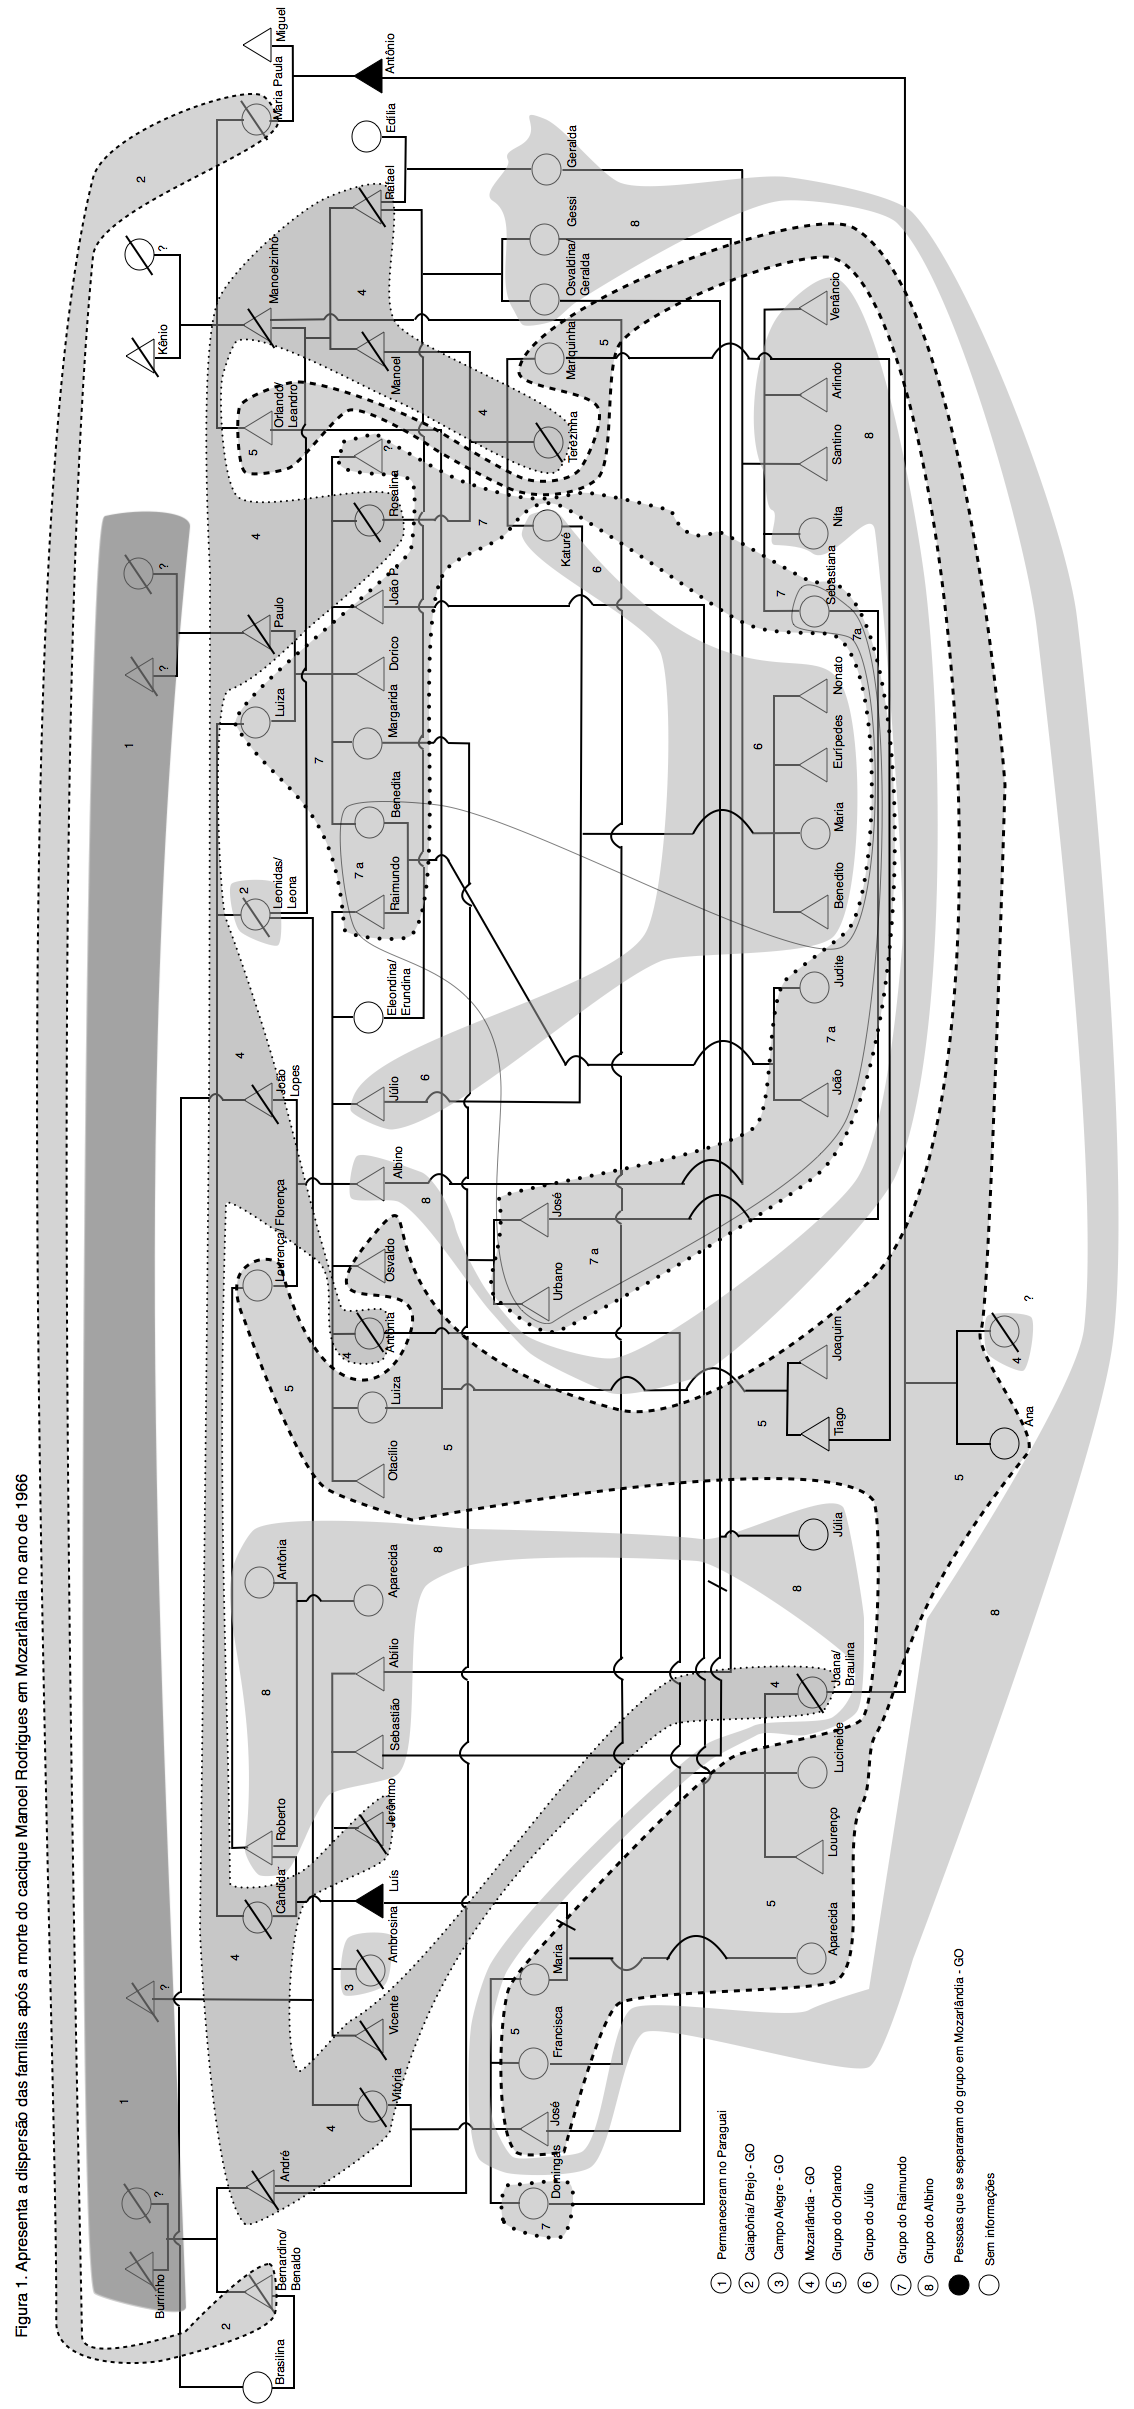
\includegraphics[width=4.798in,height=10.1016in]{livroredesguaranifinal-img9.png}
 

Ao obter not\'icias da passagem de seus parentes, o \'ultimo grupo a
chegar \`a Ilha do Bananal dividiu-se e adotou estrat\'egias
diferentes. Uma parte permaneceu na Ilha do Bananal at\'e 1978
(sombreado 8 na figura 1); outra parte (tracejado 7a na figura 1)
seguiu o mesmo itiner\'ario percorrido pelo grupo de Orlando, com o
qual se encontrou em fins da d\'ecada de 1970.

O reencontro ocorreu em Imperatriz e juntos viajaram at\'e Itinga do
Maranh\~ao. De l\'a foram para Castanhal, no Par\'a, aonde por cinco
anos trabalharam em fazendas. Nesse per\'iodo, um dos filho de
Raimundo, Jo\~ao, casou-se com sua prima de segundo grau (FZDD), Ana,
com quem tem duas filhas.

No princ\'ipio da d\'ecada de 1980 os dois grupos retornaram ao
Maranh\~ao, para a Terra Ind\'igena Guajajara Pindar\'e. No diagrama 2,
o sombreado representa os grupos de Orlando e de Raimundo, no
Maranh\~ao, entre as d\'ecadas de 1970 e 1980. Os dois grupos
aumentaram consideravelmente seu contingente populacional, no entanto,
permanecia o problema da disponibilidade de c\^onjuges.\footnote{
Diferentemente do que ocorre entre outros povos, (Fausto, 2001), a
inclus\~ao de membros estrangeiros por rapto, guerra ou
espontaneamente, n\~ao \'e comum entre os Mbya.}

  [Warning: Image ignored] % Unhandled or unsupported graphics:
%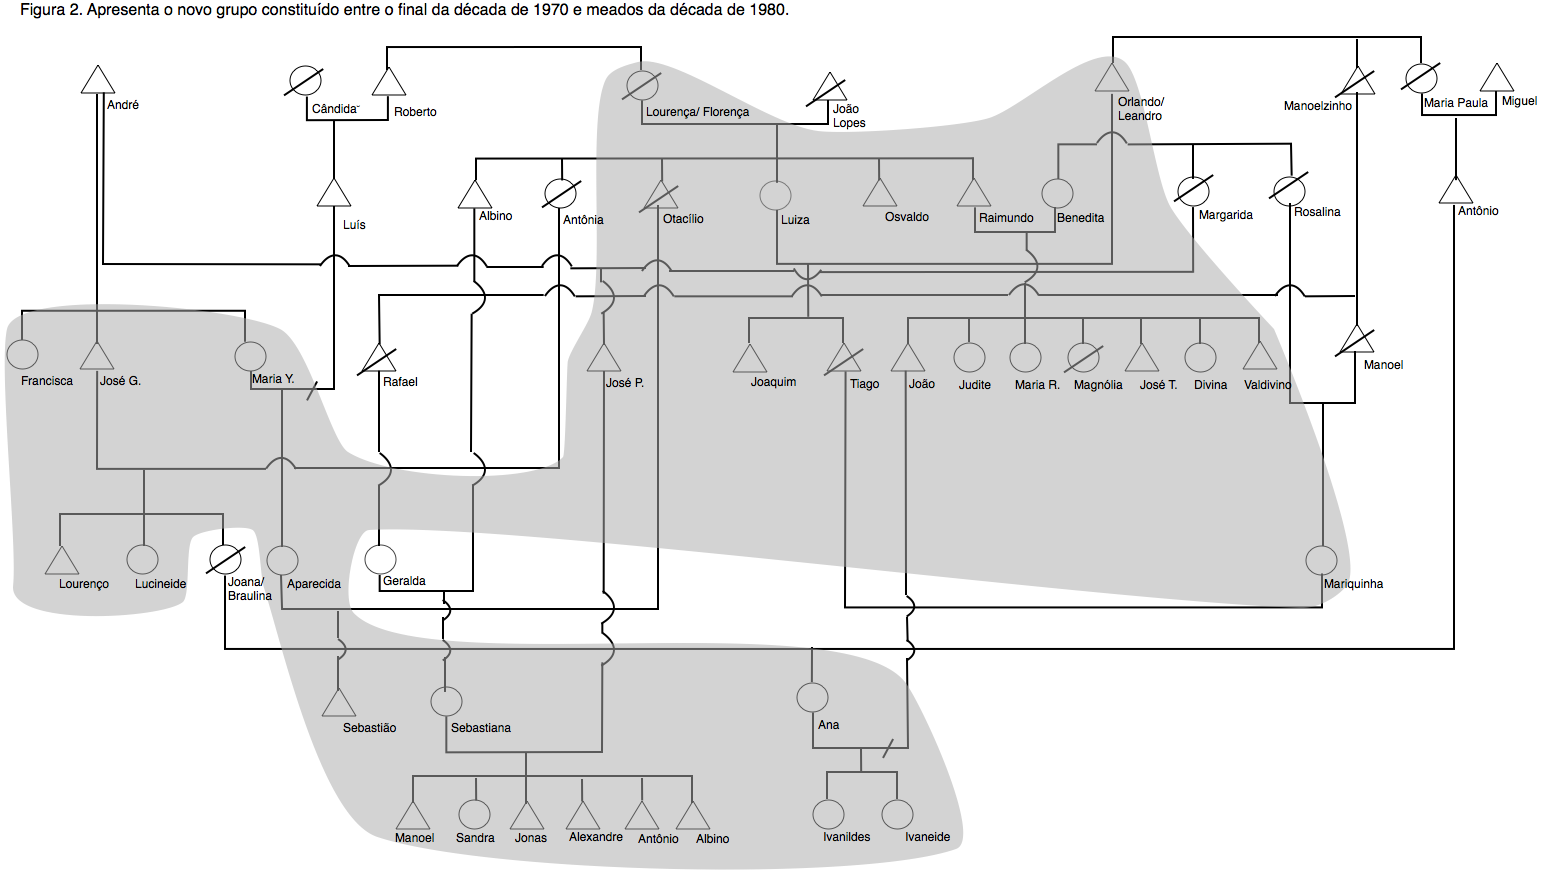
\includegraphics[width=6.6969in,height=3.798in]{livroredesguaranifinal-img10.png}
 

O conv\'ivio com os Guajajara, a despeito de haver alguns
intercasamentos, n\~ao se constituiu de forma amistosa. \`A essa
animosidade acrescenta-se a influ\^encia de pessoas n\~ao-\'indias
agindo em proveito pr\'oprio junto desses grupos\footnote{ S\~ao
in\'umeros os relatos em que n\~ao \'indios invadiam as
planta\c{c}\~oes dos Guarani para saquear ro\c{c}as ou soltavam gado
para que pastassem em suas ro\c{c}as.} e o n\~ao reconhecimento, por
parte da FUNAI, dos Guarani como povo ind\'igena.
{\textquotedblleft}Eles diziam que n\'os n\~ao pod\'iamos ficar l\'a,
porque \'eramos paraguaios{\textquotedblright} (Jo\~ao Wera). 

Em meados da d\'ecada de 1980, um padre chamado Carlo Bialli tomou
conhecimento da situa\c{c}\~ao vivida pelos Mbya no Maranh\~ao e gravou
em uma fita cassete a fala de um cacique da aldeia Itariri, conhecido
como Ant\^onio Branco --- em que ele contava sobre os Guarani no
Sudeste --- e apresentou a grava\c{c}\~ao a Orlando e Raimundo, na
tentativa de convenc\^e-los a irem para o Sudeste. Nesta \'epoca, o
div\'orcio entre Jo\~ao e Ana foi um dos motivos para que Jos\'e, av\^o
da jovem divorciada, resolvesse aceitar a proposta do padre.
Acompanhado das duas filhas, de um tio materno, de uma irm\~a de
Raimundo e do filho desta, o grupo chegou ao litoral sul de S\~ao Paulo
em 1987. O filho do cacique tamb\'em aceitou a oferta do padre, indo
at\'e S\~ao Paulo e, de l\'a, para o Rio Grande do Sul, de onde meses
mais tarde retornou para a Terra Ind\'igena M\~ae Maria, para onde a
fam\'ilia de seu pai se mudou no final da d\'ecada de 1980 (ver
diagrama 3).

  [Warning: Image ignored] % Unhandled or unsupported graphics:
%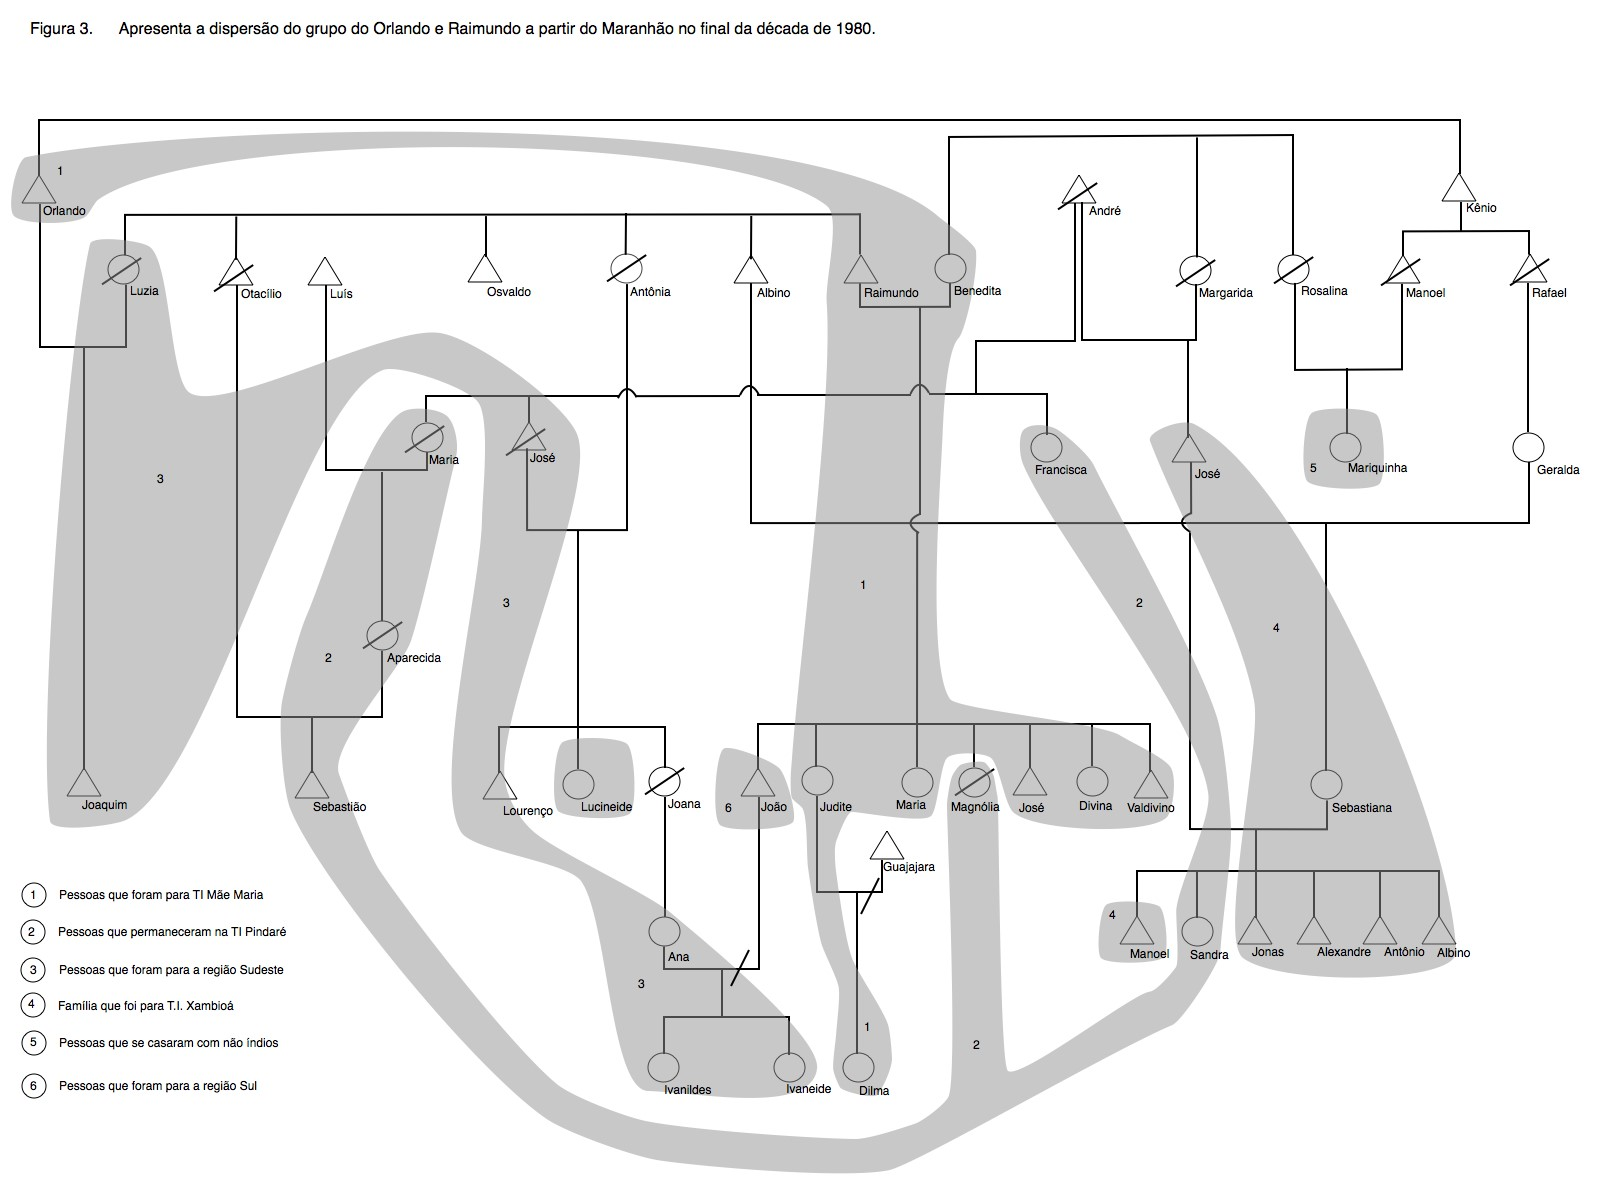
\includegraphics[width=6.6748in,height=5.0004in]{livroredesguaranifinal-img11.jpg}
 

Os contextos vividos por Albino e seu grupo apresentam uma
configura\c{c}\~ao diferente. Ap\'os nove anos na Ilha do Bananal,
vivendo em duas aldeias karaj\'a (Santa Isabel e Canoan\~a), no
in\'icio da d\'ecada de 1980 Albino se estabeleceu com a sua fam\'ilia
em Aragua\'ina, onde trabalhava em fazendas. Nesta ocasi\~ao, Maria ---
que desde o in\'icio da d\'ecada de 1970 vivia na Terra Ind\'igena
Xambio\'a --- tomou conhecimento de que seu tio paterno estava naquela
cidade e pediu ao marido que fosse busc\'a-lo. Em 1982, Albino e sua
fam\'ilia chegaram a Xambio\'a (figura 4). 

A conviv\^encia na aldeia dos Karaj\'a teve duas consequ\^encias: a
primeira foram os intercasamentos. A segunda foi a repress\~ao por
parte dos Karaj\'a, principalmente as crian\c{c}as, em forma de
zombarias e agress\~oes contra as crian\c{c}as Mbya para que n\~ao
falassem em sue pr\'oprio idioma,, mas em portugu\^es, majoritariamente
falado pelos Karaj\'a naquela Terra Ind\'igena. O trecho abaixo \'e um
excerto de uma conversa mais longa junto a Leonardo e seu tio paterno,
Ab\'ilio. 

Ab\'ilio: Meus meninos ainda falava na linguagem\footnote{ \'E como os
setentrionais se referem \`as falas no idioma guarani.} um com o outro,
assim. A\'i os outros [Karaj\'a] ficavam rindo... \'E, eles mangavam
deles a\'i. Ent\~ao com isso a\'i perdeu, ficou com vergonha de falar
tamb\'em.

Leonardo: Foi desse jeito mesmo l\'a no Xambio\'a. Quando a gente falava
na linguagem eles jogavam pedra na gente. Jogavam pedra, mangavam,
riam, \'e assim mesmo. 

Ab\'ilio: Pois \'e, por isso que os meninos perderam, perderam n\~ao,
n\~ao querem mais falar.

Leonardo: Chegamos l\'a, n\'os convers\'avamos tudo na linguagem. A\'i
l\'a mesmo, quando eu estava parando de falar na linguagem, que n\'os
cheg\'avamos junto, todo mundo assim --- velho Albino, velha Geralda,
tio Arlindo --- a\'i eu ia conversar na linguagem e eu mesmo sorria de
mim. (Ab\'ilio Karai e Leonardo Guarany, Nova Jacund\'a, 24/06/2013)

  [Warning: Image ignored] % Unhandled or unsupported graphics:
%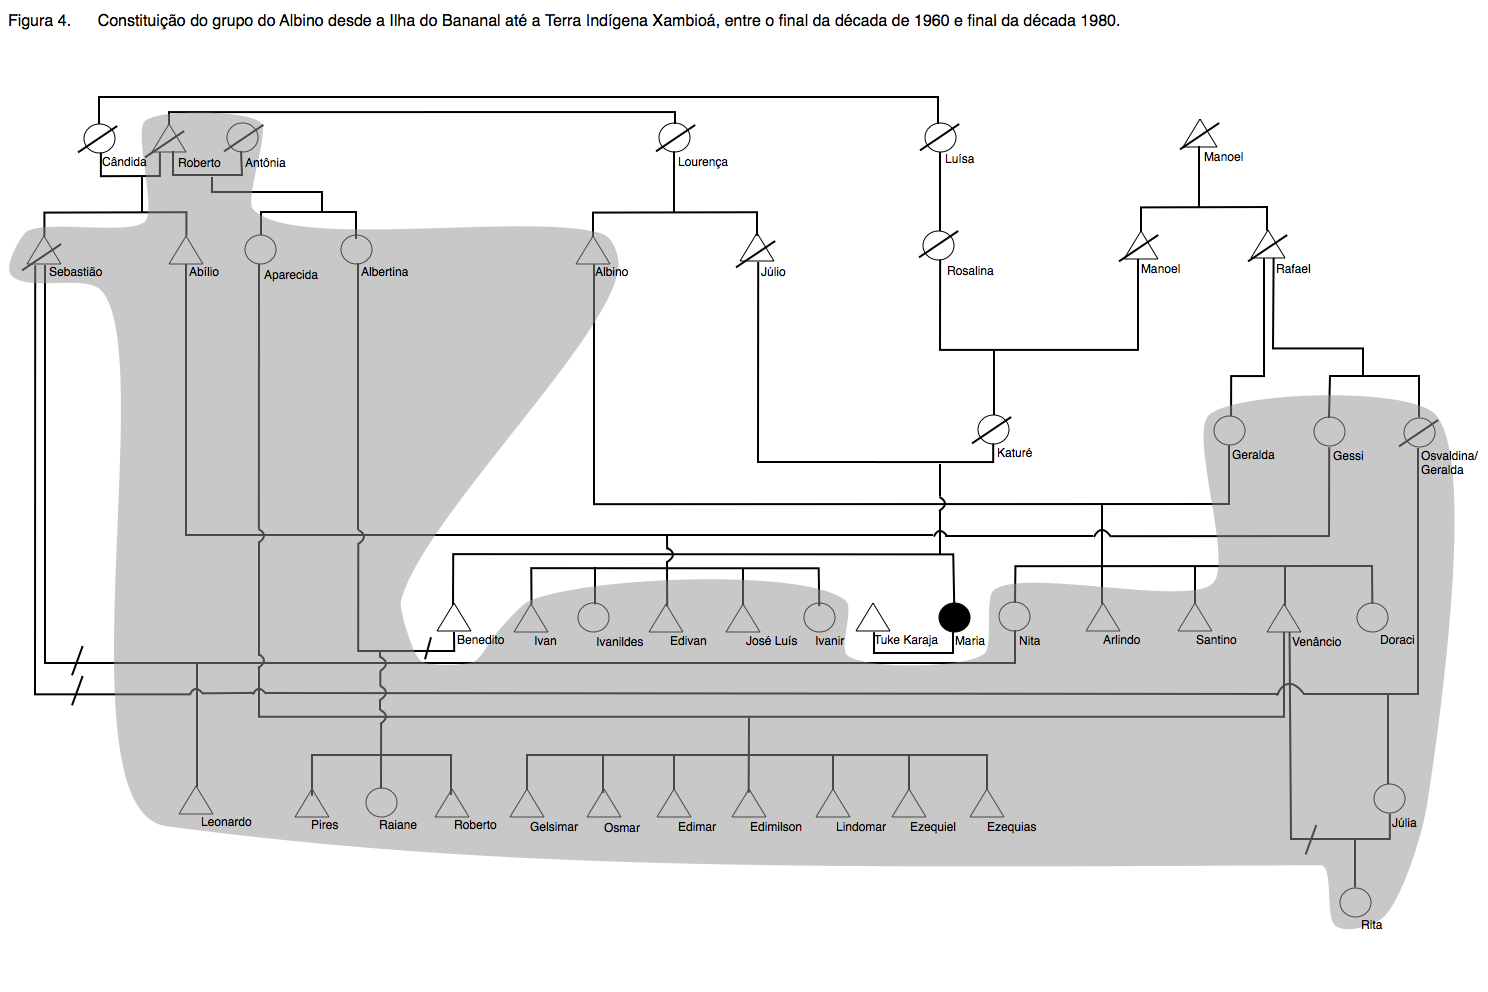
\includegraphics[width=5.9217in,height=3.8988in]{livroredesguaranifinal-img12.png}
 

\`A exce\c{c}\~ao da partida do primeiro grupo, liderado por Orlando, a
busca pelos parentes dispersos e o desejo de viverem juntos parecem ter
sido os principais orientadores dos deslocamentos pela regi\~ao Norte.
Nos relatos anteriores, esse teria sido um dos motivos que lan\c{c}aram
J\'ulio e Raimundo no encal\c{c}o do primeiro grupo. Albino, durante
anos, enviou um de seus filhos \`a procura do paradeiro de seus
irm\~aos. No entanto, foi Eur\'ipedes, filho de J\'ulio que desde o
in\'icio da d\'ecada de 1970 vivia na Terra Ind\'igena M\~ae Maria, que
foi ao Maranh\~ao levar a not\'icia de que Albino estava na Terra
Ind\'igena Xambio\'a.

Nesta ocasi\~ao, Sebastiana manifestou o desejo de reencontrar seus
pais. Acompanhada do marido e dos filhos, no final da d\'ecada de 1980
chegaram a Xambio\'a, onde viveram at\'e 1996. Como \'e poss\'ivel
observar na figura 3, entre meados e final da d\'ecada de 1980 as
fam\'ilias que estavam no Maranh\~ao percorreram itiner\'arios bem
distintos: uma parcela (sombreado 2) casou com os Guajajara, e mais
tarde a ela se uniram outros parentes; outra, sombreado 3, se mudou
para o estado de S\~ao Paulo; a fam\'ilia marcada com o sombreado 4 foi
para Xambio\'a; o sombreado 1 mostra Orlando, que acompanhou a
fam\'ilia de Raimundo at\'e a TI Gavi\~ao M\~ae Maria, nas proximidades
de Marab\'a; e o sombreado 6, uma pessoa que foi para o sul do pa\'is.

As unidades familiares, nessa ocasi\~ao, bem reduzidas, se veem diante
da dificuldade de se perpetuarem de maneira end\'ogena. Aos Mbya, que
at\'e a chegada ao Maranh\~ao se recusavam a contrair matrim\^onios com
pessoas n\~ao-\'indias ou de outras etnias, imp\~oe-se a necessidade de
abertura ao exterior. Uma das filhas de Raimundo se casou com um homem
Akewara; outra, com um homem Gavi\~ao, e o filho mais velho foi para o
Rio Grande do Sul. 

A conviv\^encia com os Gavi\~ao foi marcada por altos e baixos.
Inicialmente esses \'ultimos acolheram os Mbya, interessados nas
possibilidades matrimoniais com as mulheres rec\'em chegadas. Mas se
tornaram hostis diante da n\~ao efetiva\c{c}\~ao plena da afinidade,
seguida de um acidente que culminou na morte de um homem Gavi\~ao
durante o trabalho de abertura de uma ro\c{c}a para os Mbya.

Decorrido certo tempo, as rela\c{c}\~oes voltaram a se estreitar por
iniciativa dos Gavi\~ao, novamente interessados nas mulheres Mbya. A
n\~ao celebra\c{c}\~ao de alian\c{c}as entre os dois grupos resultou em
saques, pelos Gavi\~ao, \`as ro\c{c}as Mbya. Diante da grave
situa\c{c}\~ao de conflito, Raimundo, com ajuda da ONG Centro de
Trabalho Indigenista, adquiriu uma \'area de fazenda, na qual fundaram
a Terra Ind\'igena Nova Jacund\'a, em 1996. O final do per\'iodo em que
viveram entre os Gavi\~ao e o in\'icio da ocupa\c{c}\~ao de Nova
Jacund\'a foi marcado por intenso estreitamento das rela\c{c}\~oes
entre as pessoas que habitavam Xambio\'a e a fam\'ilia de Raimundo,
ap\'os um per\'iodo de dispers\~ao de cerca de 30 anos.

No entanto, o tempo permanecido em aldeias de outras etnias tiveram
consequ\^encias sobre os grupos futuros: a primeira foi a fixa\c{c}\~ao
de c\^onjuges Mbya nas terras ind\'igenas Xambio\'a e M\~ae Maria
devido aos casamentos inter\'etnicos com os Karaj\'a e com os Gavi\~ao.
A segunda foi o abandono e a consequente perda do idioma. Vivendo entre
grupos que apenas algumas pessoas falavam a l\'ingua materna, as
gera\c{c}\~oes mbya mais novas se viram cerceadas de falar, no
dom\'inio p\'ublico, o seu idioma. A l\'ingua portuguesa se tornou o
idioma falado majoritariamente, e o guarani se limitou ao espa\c{c}o
dom\'estico, das gera\c{c}\~oes mais velhas entre si e destas \`as mais
novas. No entanto, os filhos de casamentos inter\'etnicos compreendem e
falam apenas o idioma portugu\^es. Contudo, o reencontro das fam\'ilias
em Nova Jacund\'a ampliou as possibilidades matrimoniais internas e
criou um n\'ucleo mbya, que, no que se refere ao idioma, vem alterando
essas consequ\^encias.

Em 2004, poucos anos ap\'os a morte de Raimundo, alguns conflitos
internos for\c{c}aram o grupo de Albino a retornar \`a sua antiga sede,
a Terra Ind\'igena Xambio\'a. Todavia, essa ruptura n\~ao foi absoluta
e o fluxo de pessoas mbya entre as duas aldeias continuou frequente,
inclusive com fins matrimoniais.

Potencialmente afins

A sess\~ao anterior tratou dos deslocamentos empreendidos desde o
noroeste de Goi\'as at\'e os contextos em que vivem atualmente os Mbya,
por isso sua caracter\'istica mais descritiva. Nesta sess\~ao ser\'a
dispensada aten\c{c}\~ao ao problema colocado pelo reduzido n\'umero de
pessoas que compunham cada unidade em deslocamento, ampliado pelo fato
de essas pessoas serem parentes entre si.

Para os Mbya n\~ao existe uma categoria de pessoas para a qual o
casamento seja prescrito. Entre os meridionais afirma-se que uma pessoa
deve casar com algu\'em que n\~ao seja classificado como parente,
categoria que inclui os tios e tias maternos e paternos, os primos
cruzados e paralelos e os filhos e filhas de irm\~aos e irm\~as reais
de ego. Indiretamente, a categoria parente pode incluir qualquer pessoa
que esteja relacionada por cogna\c{c}\~ao a uma das categorias
anteriores, mas esses s\~ao classificados como parentes distantes e o
casamento entre tais pessoas, embora criticado, n\~ao \'e
raro\footnote{ \'E necess\'ario destacar aqui uma distin\c{c}\~ao entre
parentes, de um lado, e consangu\'ineos e afins, de outro. As
categorias nativas que traduzimos por parente --- xeretar\~a ou
xeregua{\textquoteright}i --- possuem, para os Mbya, um campo
sem\^antico vasto, podendo ser aplicadas desde pessoas com v\'inculos
cogn\'aticos at\'e os demais concidad\~aos, fen\^omeno recorrente entre
os amer\'indios (Rivi\'ere, 2001; Vila\c{c}a, 1992; Pissolato, 2007;
Mello, 2006; Silva, 2009).}. 

{\textquotedblleft}Aqui n\'os casamos com primos de segundo
grau{\textquotedblright} afirmou-me uma mulher com quem eu conversava
em Nova Jacund\'a. Este tipo de casamento, obl\'iquo, revela, para o
contexto Mbya, uma caracter\'istica comum a outros contextos
amaz\^onicos, como entre os Parakan\~a, por exemplo, (Fausto, 1991;
2001). Por\'em, diferentemente destes \'ultimos, os casamentos n\~ao
s\~ao entre irm\~ao da m\~ae e filha da irm\~a (MB/ZD), modelo
cl\'assico do avunculato amaz\^onico. Entre os Mbya, n\~ao \'e o
irm\~ao da m\~ae que \'e convertido em genro de sua pr\'opria irm\~a,
mas o primo ou primos cruzados ou paralelos que, classificado como
irm\~ao ou irm\~a, \'e transformado em genro ou nora. Diferentemente do
caso Parakan\~a, n\~ao \'e uma rela\c{c}\~ao entre tios e sobrinhas
(Fausto, 1995), mas entre pessoas que s\~ao classificadas como av\^os e
netas. Os Mbya setentrionais classificam os filhos de irm\~aos
classificat\'orios n\~ao necessariamente como sobrinhos, mas como
netos.

Dos oito casamentos atuais em Nova Jacund\'a, quatro se deram entre
pessoas relacionadas segundo as classes acima. Em Xambio\'a s\~ao dois
casos, e se retrocedermos um pouco mais no tempo, encontraremos este
modelo de casamento. Tudo se passa como se os Mbya inclu\'issem no polo
da afinidade virtual todas as pessoas que n\~ao perten\c{c}am \`as
categorias acima.

Entre os Mbya meridionais, n\~ao \'e raro encontrarmos esse tipo de
casamento, por\'em tal como em Xambio\'a, onde o menu \'e mais variado,
os arranjos conjugais tamb\'em podem s\^e-lo. O que se conclui \'e que
para os Mbya s\~ao interditas as categorias pai, m\~ae, irm\~ao,
irm\~a, tio, tia maternos e paternos, e primos e primas de primeiro
grau. Esse ponto foi explicitamente enunciado, em portugu\^es, pelo
cacique quando manifestava preocupa\c{c}\~ao por n\~ao haver c\^onjuges
dispon\'iveis em Nova Jacund\'a. As mulheres citadas no trecho abaixo
s\~ao as suas irm\~as reais.

Eu fico preocupado porque daqui a pouco n\'os vamos acabar, porque vai
ter que casar com jurua ou com outros \'indios; ent\~ao \'e melhor
casar com outros \'indios, porque aqui n\~ao tem com quem casar. V\^e
os meus filhos, com quem eles v\~ao se casar? Com as filhas da Maria?
Da Divina? E elas com quem v\~ao casar? N\~ao pode! N\'os somos
\'indios, mas n\~ao somos bichos n\~ao, a gente sabe que \'e
errado!{\textquotedblright} (Jo\~ao Wera, Nova Jacund\'a, 11/06/2012)

Em sua tese de doutorado, Mello (2006: 75) havia chamado a aten\c{c}\~ao
para esse ponto: o incesto {\textquotedblleft}considerado como uma
conduta animalesca, \'e tratado com certo
constrangimento{\textquotedblright}. No trecho acima, a conduta
incestuosa \'e o casamento entre os primos de primeiro grau. Destaco
que os Mbya, formalmente, n\~ao distinguem entre primos paralelos e
primos cruzados; isso n\~ao significa que as no\c{c}\~oes de
consanguinidade e de afinidade n\~ao constituam modelos relacionais no
socius mbya, elas ser\~ao acionadas ou negadas conforme o campo
relacional em jogo: a afinidade amaz\^onica, citando Viveiros de
Castro, {\textquotedblleft}n\~ao s\'o determinam outros referentes que
os nossos, como envolvem outros componentes{\textquotedblright} (2002:
406) . Na sequ\^encia reitera: a afinidade pode se aplicar a
rela\c{c}\~oes com estranhos, mesmo se nenhum casamento acontece; e
mais, ela se aplica sobretudo \`aqueles casamentos com os quais o
casamento n\~ao \'e uma possibilidade pertinente{\textquotedblright}
(idem: 408)

Esse problema da pertin\^encia ou n\~ao de certos casamentos \'e
fundamental. \'E conhecido na literatura antropol\'ogica hist\'orias de
pessoas que seduzidas por membros de outras esp\'ecies terminam por
irem residir no mundo dessas pessoas como afins (Vila\c{c}a, 1992,
2005; Lima, 1996). Esse tipo de transforma\c{c}\~ao n\~ao \'e estranha
aos Guarani, que a denominam jepota. Como em outros contextos
amer\'indios, ocorre quando uma pessoa, em determinadas fases da vida,
\'e seduzida por um membro de uma esp\'ecie animal e passa a tom\'a-lo
como parceiro sexual (Clastres, 1978; Macedo, 2013; Mendes J\'unior,
2009; Pissolato, 2007; Schaden, 1962 [1954]).

Outro modelo de casamento impertinente \'e aquele que se estabelece
entre pessoas Mbya e n\~ao-Mbya (jurua ou te{\textquoteright}yi). Este
tipo de casamento \'e denominado, entre os setentrionais,
jejavy\footnote{ Javy tem o significado de pecar, errar, ou equivocar
(Cadogan, 1992).  Jejavy, entre os setentrionais, possui este
significado preciso: casar-se com pessoas n\~ao-Mbya. Migliora (2014) e
Pereira (2014) abordam os casamentos entre Mbya e jurua de uma forma
positiva a partir de suas experi\^encias de campo na aldeia das
Sementes, tekoa Mbo{\textquoteright}y ty, em Niter\'oi.}. No entanto,
jejavy n\~ao se restringe apenas ao casamento, mas a qualquer tipo de
rela\c{c}\~ao sexual entre essas pessoas. O motivo de sua
impertin\^encia \'e o enfraquecimento do esp\'irito
(nhe{\textquoteright}\"e) dos pais causado pela mistura de sangue
atrav\'es da rela\c{c}\~ao sexual. Os filhos desses casamentos, entre
os setentrionais, n\~ao eram nominados\footnote{ Durante a
constru\c{c}\~ao das genealogias, apontaram-me tr\^es pessoas que n\~ao
possu\'iam nomes mbya. O motivo era claro: {\textquotedblleft}jurua
ra{\textquoteright}y ou jurua rajy{\textquotedblright} (filho ou filha
de pai jurua)  } pelo xam\~a, restando-lhes apenas o nome brasileiro.
Esse enfraquecimento, no limite, ocasiona a morte da pessoa.

Jejavy e jepota s\~ao, portanto, dois modos indesejados de rela\c{c}\~ao
com o exterior e pelas mesmas raz\~oes: a perda da verdadeira
condi\c{c}\~ao humana. A v\'itima de jepota deixa o conv\'ivio de seus
parentes e termina por viver entre os animais. A v\'itima de jejavy
tamb\'em deixa o conv\'ivio de seus parentes, n\~ao ensina o seu idioma
aos seus filhos e termina por viver como jurua ou
te{\textquoteright}yi, entre brancos ou \'indios. 

Novos encontros, novos contextos

O objetivo dessa sess\~ao \'e percorrer os fios que conectam as aldeias
setentrionais \`as meridionais, em especial Parati-Mirim e Araponga,
localizadas no munic\'ipio de Parati, no estado do Rio de Janeiro.
Vimos no diagrama 3 que as pessoas no sombreado 3 seguiram para os
estados da regi\~ao Sudeste. O que motivou essas pessoas a deixar o
conv\'ivio junto de seus parentes para seguir em dire\c{c}\~ao a terras
e pessoas que, embora guarani, eram estranhas?

Como mostrei na segunda se\c{c}\~ao, os Mbya enfrentavam uma
conviv\^encia dif\'icil entre os Guajajara. Neste mesmo per\'iodo, uma
mulher havia se separado recentemente de seu marido e, segundo relatos,
n\~ao havia com quem se casar que n\~ao fosse guajajara ou jurua. Essa
\'epoca coincidiu com a oferta do padre Bialli para que as pessoas
aceitassem a proposta de se mudarem para S\~ao Paulo. Acompanhada de
seu tio materno, Ana, suas duas filhas, e mais duas pessoas (cf. figura
3) aceitaram a oferta e entre meados e o final da d\'ecada de 1980
chegaram ao Itariri.

L\'a encontraram um grupo que recentemente deixara o oeste do Paran\'a e
seguia em dire\c{c}\~ao ao litoral. A conviv\^encia conjunta teve como
resultado o casamento entre Ana e um dos rapazes do grupo. Certo tempo
se passou at\'e que o novo grupo seguiu para o Esp\'irito Santo. As
demais pessoas que vieram do Par\'a permaneceram por um tempo no
Itariri e, mais tarde, o tio materno de Ana foi para a aldeia Krukutu,
onde reencontraria seu pai. Do Esp\'irito Santo o primeiro grupo se
mudou para duas aldeias no estado do Rio de Janeiro e posteriormente
fundaram a aldeia Parati-Mirim, em meados da d\'ecada de 1990.

O que afirmou Pissolato para os Mbya meridionais, n\~ao \'e menos
plaus\'ivel para os setentrionais: {\textquotedblleft}[...] a
movimenta\c{c}\~ao de pessoas \'e em si o modo de realiza\c{c}\~ao do
parentesco [...] e a express\~ao da atitude mais fundamental da busca
pessoal de satisfa\c{c}\~ao{\textquotedblright} (2007: 59);
{\textquotedblleft}se n\~ao se fica alegre entre parentes, deve-se
deix\'a-los para buscar parentes outros{\textquotedblright} (Idem).

Paralelamente \`a partida do primeiro grupo, Jo\~ao, o ex-marido da
jovem, deixou a sua fam\'ilia e seguiu em dire\c{c}\~ao ao Sudeste. Num
primeiro momento seguiu de Angra dos Reis at\'e o Rio Grande do Sul, de
onde retornou a Marab\'a. Mais tarde, acompanhado de Jos\'e, o av\^o de
sua ex-esposa, e de um primo seu chegou a S\~ao Paulo, onde os deixou e
seguiu novamente para o Rio Grande do Sul. Em Porto Alegre conheceu
algumas pessoas da aldeia Pacheca, localizada no extremo sul do estado,
que o convidaram para ir at\'e l\'a. Pouco ap\'os sua chegada a essa
aldeia, casou-se com uma jovem e, em seguida, convenceu a fam\'ilia de
sua esposa a acompanh\'a-lo at\'e o Rio de Janeiro, onde se encontravam
alguns parentes de seu sogro.

No princ\'ipio da d\'ecada de 1990, chegaram a Angra dos Reis, e mais
tarde a Ubatuba. Nesta \'ultima aldeia deixou sua mulher gr\'avida e
partiu para a aldeia Rio Branco, no estado de S\~ao Paulo, onde se
casaria novamente e teria outro filho. O grupo que deixara em Ubatuba
se estabeleceu, em meados da d\'ecada de 1990, na aldeia Araponga, no
sul do Rio de Janeiro. Ap\'os cinco anos na aldeia Rio Branco, este
homem decidiu retornar ao Par\'a, indo para a terra que finalmente
pertencia aos seus parentes.

A an\'alise de Pissolato atinge aqui sua import\^ancia comparativa. Do
ponto de vista das pessoas envolvidas, a perman\^encia na regi\~ao
Norte representava um quadro desfavor\'avel ao estabelecimento de novas
alian\c{c}as de parentesco, visto que as oportunidades eram restritas.
A busca de outros contextos que possibilitassem a realiza\c{c}\~ao do
parentesco despontava como objetivo pessoal de satisfa\c{c}\~ao. A
recusa em incorrer em jejavy, casamentos cujas possibilidades n\~ao
s\~ao pertinentes, motivou esses n\'ucleos a caminhar; ou como colocou
a autora, a buscar parentes outros. 

A fixa\c{c}\~ao de fam\'ilias em Parati-Mirim, bem como o nascimento de
filhos em Araponga e Rio Branco, conecta as aldeias setentrionais e
meridionais. O fluxo de pessoas entre elas n\~ao \'e t\~ao intenso
quanto o \'e entre as aldeias meridionais, por\'em existe. Mais intenso
\'e a circula\c{c}\~ao de not\'icias e o desejo de fazer com que os de
um lado saibam o que ocorre do outro lado. A dist\^ancia entre as duas
regi\~oes talvez seja, na atualidade, a maior dificuldade para essa
circula\c{c}\~ao de pessoas. Aquele que se desloca, ao mesmo tempo que
deseja buscar a satisfa\c{c}\~ao de novas possibilidades de parentesco,
lamenta-se por deixar os parentes. 

Ter ou n\~ao parentes em um lugar \'e sempre posto em evid\^encia
durante as situa\c{c}\~oes de conflito. Em 2007, o cacique de Nova
Jacund\'a foi at\'e Parati-Mirim com o objetivo de levar pessoas para a
sua aldeia. Acompanharam-no uma fam\'ilia cujo marido era primo do
cacique, e a sobrinha da esposa deste primo. A saudade que a mulher
deste primo sentia de seus parentes (ndovy{\textquoteright}ai), a morte
de dois filhos rec\'em-nascidos e a diferen\c{c}a de contextos entre as
duas regi\~oes foram fatores decisivos para que essa fam\'ilia voltasse
para o Sudeste. No entanto, a sobrinha, que se casara com um rapaz em
Nova Jacund\'a, permaneceu. Com o passar do tempo, a saudade de seus
parentes e alguns conflitos com seus afins trouxeram-na de volta \`a
aldeia Krukutu, em S\~ao Paulo.

Nota Final

Ao longo deste artigo procurei mostrar como se configura o contexto
etnogr\'afico dos Mbya no norte do Brasil. Nesse esfor\c{c}o, destaquei
dois temas cl\'assicos tanto na antropologia em geral como na
etnografia dos povos guarani: o parentesco e a busca da terra sem mal.
Acompanhar os movimentos migrat\'orios e a mobilidade nessas regi\~oes
significou percorrer os fios de uma complexa rede de parentesco, sem o
que corremos o risco de enxergar os Mbya como pequenas ilhas num oceano
de etnias.

O caso setentrional revelou-se consp\'icuo no que se refere ao estudo do
parentesco, principalmente quando comparados a outros modelos
amaz\^onicos; penso aqui nos desenvolvimentos trazidos por Viveiros de
Castro (1993; 1996; 2002); Lima (1996) e Vila\c{c}a (2005), excelentes
ferramentas para analisarmos o tema da afinidade justamente ali onde
ela existe como pot\^encia --- jepota e jejavy. Paralelamente, este
contexto torna vis\'ivel uma forma matrimonial menos percept\'ivel
entre os meridionais: o casamento obl\'iquo entre primos de segundo
grau.

Ao longo deste trabalho o termo migra\c{c}\~ao gozou do mesmo estatuto
que lhes deram Nimuendaju (1987 [1914]), Clastres (1978 [1975]) e
Schaden (1962 [1954]): o deslocamento de um grupo de pessoas conduzido
por um xam\~a em busca da terra sem mal. Sendo assim, o per\'iodo de
migra\c{c}\~ao est\'a compreendido entre a sa\'ida do Paraguai, na
d\'ecada de 1930 e a morte do segundo xam\~a, em meados da d\'ecada de
1960, em Goi\'as.

Aos deslocamentos para a {\textquotedblleft}visita\c{c}\~ao entre
parentes, busca por c\^onjuges e outra diversidade de motivos
implicados nos movimentos populacionais do grupo{\textquotedblright}
mantenho o termo proposto por Garlet: mobilidade (Garlet, 1997: 16 apud
Pissolato, 2007: 97). Ap\'os o falecimento do xam\~a, o esfacelamento e
a dispers\~ao do grupo ao longo do interfl\'uvio Araguaia-Tocantins
possui uma caracter\'istica amb\'igua. Inicialmente oscila entre a
busca da terra sem mal e a procura por parentes, afirmando cada vez
mais essa \'ultima caracter\'istica. 

Diante disso, diferentemente de Garlet, que classifica as
migra\c{c}\~oes como variantes da mobilidade, neste trabalho os dois
termos dever\~ao ser mantidos em separado. Essa op\c{c}\~ao se
justifica pelo fato da mobilidade, como acima definida, dar-se entre
territ\'orios guarani. As diversas terras ind\'igenas Guarani
existentes ao longo das regi\~oes Sul e Sudeste do Brasil, entre as
quais \'e poss\'ivel observar rela\c{c}\~oes de parentesco
pr\'e-estabelecidas que muitas das vezes orientam os deslocamentos de
pessoas ou grupo. Diferentemente, os Guarani que se deslocaram em
dire\c{c}\~ao \`a regi\~ao Norte foram orientados pelo desejo de se
chegar \`a terra sem mal, localizada na dire\c{c}\~ao do sol nascente,
n\~ao contando, portanto, com nenhuma rede de parentesco ou de outras
rela\c{c}\~oes quaisquer pr\'e-estabelecidas.

Refer\^encias

ALBERNAZ, Adriana Cristina Repelevicz. Antropologia, hist\'orias e
temporalidades entre os Ava-Guarani de Oco{\textquoteright}i (PR). Tese
de Doutorado. Florian\'opolis: UFSC, 2009.

CADOGAN, Leon. Dicionario mbya-guarani-castellano. Asunci\'on: Ceaduc-
Cepag, 1992.

CAPDEVILA, Luc. {\textquotedblleft}La guerre du Chaco Tierra adentro
d\'econstruire la representation d{\textquoteright}un conflit
international{\textquotedblright}. In: Capdevila, Luc Capdevila;
Comb\`es, Isabelle; Richard, Nicolas; Barbosa, Pablo. Les hommes
transparents: indiens et militaires dans la guerre du Chaco
(1932-1935). Rennes: PUR, 2010.

CHAMORRO, Graciela.  A espiritualidade guarani: uma teologia amer\'india
da palavra. S\~ao Leopoldo: Ed. Sinodal, 1998.

CLASTRES, H\'el\`ene. A terra sem mal: o profetismo tupi-guarani. S\~ao
Paulo: Brasiliense, 1978.

FAUSTO, Carlos. Os Parakan\~a. Parentesco e avunculato.
Disserta\c{c}\~ao de Mestrado. Rio de Janeiro: PPGAS-UFRJ, 1991.

{}---{}---{}---{}---{}---. {\textquotedblleft}De primos e sobrinhas:
terminologia e alian\c{c}a entre os Parakan\~a (Tupi) do
Par\'a{\textquotedblright}. Viveiros de Castro, Eduardo (org.).
Antropologia do parentesco: estudos amer\'indios. Rio de Janeiro:
Editora UFRJ, 1995.

{}---{}---{}---{}---{}---. Inimigos Fi\'eis. S\~ao Paulo: Edusp, 2001.

HEURICH, Guilherme Orlandini. Outras alegrias: parentesco e festas mbya.
 Disserta\c{c}\~ao de Mestrado. Rio de Janeiro: PPGAS-Museu Nacional,
2011.

LADEIRA, Maria In\^es. O caminhar sobre a luz: o territ\'orio mby\'a \`a
beira do oceano. Disserta\c{c}\~ao de Mestrado. S\~ao Paulo: PUC-SP,
1992.

\_\_\_\_\_\_\_\_\_\_. Espa\c{c}o geogr\'afico guarani-mbya: Significado,
constitui\c{c}\~ao e uso. S\~ao Paulo: Edusp, 2008.

LIMA, T\^ania Stolze. O dois e seu m\'ultiplo: reflex\~oes sobre o
perspectivismo em uma cosmologia tupi. Mana 2(2), 1996.

MACEDO, Val\'eria. Nexos da diferen\c{c}a. Cultura e afec\c{c}\~ao em
uma aldeia guarani na Serra do Mar. Tese de Doutorado. S\~ao Paulo:
PPGAS-USP, 2009.

{}---{}---{}---{}---{}---. De Encontros nos Corpos Guarani. Ilha 15(2),
2013.

MELI\`A, Bartolomeu. El Guarani: experiencia religiosa. Asunci\'on:
Ceaduc-Cepag, 1991

MELLO, Fl\'avia Cristina de. Aetch\'a Nhaderukuery karai retar\~a: Entre
deuses e animais: xamanismo, parentesco e transforma\c{c}\~ao entre os
Chirip\'a e Mby\'a Guarani. Tese de Doutorado. Florian\'opolis:
PPGAS-UFSC, 2006.

MENDES J\'UNIOR, Rafael Fernandes. Os animais s\~ao muito mais do que
algo somente bom para comer. Disserta\c{c}\~ao de Mestrado. Niter\'oi:
PPGA-UFF, 2009.

MIGLIORA, Amanda Alves. Inventando outros: desdobramentos de um contato
multifacetado. Disserta\c{c}\~ao de Mestrado. Rio de Janeiro:
PPGAS-Museu Nacional, 2014.

NIMUENDAJU, Curt Unkel. As lendas de cria\c{c}\~ao e destrui\c{c}\~ao do
mundo como fundamentos da religi\~ao apapoc\'uva-guarani. S\~ao Paulo:
Ed. Hucitec, 1987 [1914].

PEREIRA, Vicente Cretton. Aqueles que n\~ao vemos: uma etnografia das
rela\c{c}\~oes de alteridade entre os Mbya Guarani. Disserta\c{c}\~ao
de Mestrado. Niter\'oi: PPGA-UFF, 2014.

PIERRI, Daniel Calazans. O perec\'ivel e o imperec\'ivel: l\'ogica do
sens\'ivel e corporalidade no pensamento guarani-mbya.
Disserta\c{c}\~ao de Mestrado. S\~ao Paulo: PPGAS-USP, 2013.

PISSOLATO, Elizabeth. A dura\c{c}\~ao da pessoa: mobilidade, parentesco
e xamanismo mbya (guarani). S\~ao Paulo: Unesp, ISA; Rio de Janeiro:
NuTi, 2007.

RIVI\`ERE, Peter. Indiv\'iduo e Sociedade na Guiana. S\~ao Paulo: Edusp,
2001.

SCHADEN, Egon. Aspectos fundamentais da cultura guarani. S\~ao Paulo:
Difel, 1962 [1954]. 

SILVA, Evaldo Mendes da. Folhas ao vento: a micromobilidade de grupos
Mbya e Nhand\'eva (Guarani) na Tr\'iplice Fronteira. Cascavel:
Edunioeste, 2009.

VILA\c{C}A, Aparecida. Comendo como gente. Rio de Janeiro: ANPOCS/Ed.
UFRJ, 1992.

{}---{}---{}---{}---{}---. Chronically unstable bodies: reflections on
Amazonian corporalities. Journal of the Royal Anthropological Institute
11(3), 2005.

VIVEIROS DE CASTRO, Eduardo (1986). Arawete: os deuses canibais. Rio de
Janeiro: Jorge Zahar/ANPOCS, 1986.

{}---{}---{}---{}---{}---. {\textquotedblleft}Alguns Aspectos da
Afinidade no Dravidianato Amaz\^onico{\textquotedblright}. In: Viveiros
de Castro, Eduardo \& Carneiro da Cunha, Manuela (orgs.). Amaz\^onia:
etnologia e hist\'oria Ind\'igena. S\~ao Paulo: NHII-USP/Fapesp, 1993.

{}---{}---{}---{}---{}---. {\textquotedblleft}Atua\c{c}\~ao e
contra-efetua\c{c}\~ao do Parentesco{\textquotedblright}. In: A
inconst\^ancia da alma selvagem. S\~ao Paulo: Cosac Naify, 2002.

H\'a a dificuldade de tradu\c{c}\~ao de pensamentos, que \'e mais
intensa quando precisamos de um discurso para se fazer ouvir pelos
ruralistas e por representantes do Estado. Como a gente pode conseguir
expressar essas diferen\c{c}as de modo que possa ser comunicado para os
n\~ao antrop\'ologos? O tema da terra para os Guarani est\'a em
liga\c{c}\~ao com muitas outras terras. Aprender com os Guarani sobre a
comunica\c{c}\~ao entre essas terras talvez possa nos ajudar a pensar a
comunica\c{c}\~ao com gente que vive nessa terra mas que parece viver
em outra! H\'a v\'arias terras, h\'a a dos ruralistas e a da maioria da
popula\c{c}\~ao que n\~ao sabe quase nada sobre os \'indios com os
quais convive. H\'a muitos paulistas que n\~ao sabem que existem
aldeias grandes em S\~ao Paulo. Existem v\'arios espa\c{c}os a ocupar
entre essas terras. -- Ana Mar\'ia Ramo y Affonso

Os Mbya-Guarani de Misiones frente \`a Ley del Aborigen nos anos 1980

Donatella Schmidt\footnote{* Docente na Universidade de P\'adua,
It\'alia.}

O contexto

Misiones, Argentina: faixa de terra encravada entre Paraguai e Brasil,
povoada por muitos grupos de migrantes, mas tamb\'em territ\'orio
historicamente habitado pelos Guarani. Prova disso s\~ao as ru\'inas
das miss\~oes jesu\'iticas (1609-1773), onde a criatividade ind\'igena
deixou marcas. No final da d\'ecada de 1980, quando realizei minha
pesquisa junto aos Guarani, o Governo da prov\'incia de Misiones
aprovou uma lei relativa aos povos ind\'igenas que apresentava aspectos
inovadores. A Ley del Aborigen 2435/1987, antes de mais nada,
reconhecia os direitos territoriais das terras ocupadas pelo povo
guarani de Misiones como um conjunto, e n\~ao como demandas de aldeias
espec\'ificas. Reconhecia assim o car\'ater din\^amico das comunidades,
ocupadas em um cont\'inuo movimento de cis\~oes e recomposi\c{c}\~oes,
mas que se conectavam em uma rede de parentesco, conhecimentos,
articula\c{c}\~oes pol\'iticas e outras ordens de troca. Naquela
\'epoca, haviam cerca de 35 aldeias mbya-guarani, somando um total
aproximado de 3.500 pessoas espalhadas nos quase 30 mil
km{\texttwosuperior} da prov\'incia. Na regi\~ao norte, a \'area se
estendia \`as proximidades das cataratas do Igua\c{c}u e, ao sul, perto
de Posadas, a capital da prov\'incia.

Outro aspecto inovador foi o car\'ater participativo no processo de
promulga\c{c}\~ao dessa lei, produto de uma sinergia entre
lideran\c{c}as guarani, uma professora e estudantes de antropologia da
Universidade de Misiones\footnote{ Poucos anos antes, estudantes da
mesma Universidade tinham desaparecido para sempre por terem se
engajado ao lado de classes marginalizadas nos bairros pobres e por
terem se apresentado como pessoas de esquerda frente ao governo militar
que estava no poder (1976-1983).}, contando inclusive com apoio do
Partido Radical, naquela \'epoca no governo da Prov\'incia. 

O debate

O interesse levantado pela aprova\c{c}\~ao da Ley del Aborigen foi
surpreendente e levou a popula\c{c}\~ao n\~ao ind\'igena da regi\~ao de
Missiones a uma longa s\'erie de debates, que pude acompanhar durante
minha perman\^encia na regi\~ao. Havia aqueles que argumentavam a favor
da cria\c{c}\~ao de uma lei que reconhecia o povo guarani como
categoria jur\'idica distinta e aqueles que achavam tal divis\~ao
inconsistente com a Constitui\c{c}\~ao argentina, que n\~ao legitimava
tratamentos diferenciados em raz\~ao da origem cultural de seus
cidad\~aos\footnote{ Para maiores informa\c{c}\~oes sobre esse
contexto, ver Schmidt 1994.}. 

Todavia, o debate n\~ao ficou restrito aos n\~ao ind\'igenas. Os Guarani
tamb\'em discutiam as transforma\c{c}\~oes que esse reconhecimento
jur\'idico traria. A lei precisava ser lida, entendida, regulamentada e
dotada de um estatuto. Por isso, a Divisi\'on Abor\'igenes, \'org\~ao
do governo provincial respons\'avel pela quest\~ao ind\'igena, tinha se
colocado \`a disposi\c{c}\~ao para trabalhar conjuntamente com as
comunidades mbya-guarani interessadas pela lei. Dois ter\c{c}os do
total da popula\c{c}\~ao guarani na regi\~ao demonstraram interesse,
participando nas assembleias organizadas por esse \'org\~ao. 

A primeira dessas assembleias aconteceu em Yaveriry em julho de 1987,
logo depois da aprova\c{c}\~ao da lei: cerca de duzentos Mbya, formando
pequenos grupos em um espa\c{c}o aberto, em uma manh\~a radiante de
inverno, com o c\'eu azul intenso, as folhas brilhantes, a terra
vermelha.  Assim que os representantes do governo desceram de uma van,
os representantes dos Mbya dispuseram-se rapidamente em um
semic\'irculo, prontos para come\c{c}ar. Lorenzo Ramos, lideran\c{c}a
da aldeia Mbarangatu, tomou a palavra primeiro, falando \`a assembleia
com voz alta, em mbya, andando pra c\'a e pra l\'a naquela forma
peculiar que mais tarde terei come\c{c}ado a conhecer:

Quero que voc\^es entendam porque estamos aqui. O Governo finalmente
reconheceu nossos direitos, nos deu essa lei, ou melhor, n\'os mesmos
fizemos essa lei e eles a reconheceram. Temos que agradecer o
governador e o bispo que se preocuparam em nos dar a lei. Agora, n\'os
os agradecemos e depois pedimos para eles irem embora. Se a lei passou,
\'e para que seja em nosso benef\'icio e, portanto, deixemos de lado o
governo e o bispo para come\c{c}armos a falar dos nossos problemas.
Mas, como primeira coisa, deixemos de lado os brancos, que fiquem
longe, longe... Hoje voc\^es est\~ao aqui para decidir se est\~ao de
acordo em permanecer com a lideran\c{c}a atual ou se querem mudar.
N\~ao tenho nada pessoal contra ele, mas falta pouco para que ele morra
e ainda n\~ao quer deixar a chefia, fica segurando-a.

O duplo pedido formulado por Loren\c{c}o Ramos \'e claro: que as
institui\c{c}\~oes n\~ao ind\'igenas ficassem de lado, n\~ao intervindo
nos assuntos ind\'igenas, e que o velho Dionisio Duarte, at\'e ent\~ao
reconhecido cacique geral de todas as comunidades mbya-guarani de
Misiones, deixasse o cargo que ele, Lorenzo, assumiria. Nas longas
horas daquela assembleia em Yaveriry, como nas assembleias seguintes,
falou-se pouco da lei e de seu conte\'udo, pois segundo os Mbya seria
necess\'ario primeiro resolver a disputa pela lideran\c{c}a. De fato,
Lorenzo e Duarte a queriam.

Ambos os l\'ideres consideravam que dispunham de legitimidade para o
comando em fun\c{c}\~ao de sua posi\c{c}\~ao nas redes de parentesco. O
av\^o de Duarte por parte de m\~ae tinha vindo do Paraguai no
come\c{c}o do s\'eculo XX, tornando-se o chefe das comunidades locais;
em seguida este teria passado a lideran\c{c}a ao filho, logo falecido
de var\'iola, e ent\~ao ao irm\~ao da m\~ae de Duarte. Assim, v\'arios
parentes, sempre do lado materno at\'e que ele veio a ser nomeado
cacique geral de Misiones. Segundo seu relato, isso ocorreu em 1969, em
Campo Grande, durante uma aty guazu, assembleia onde estavam reunidos
dezoito chefes locais e quatro pa{\textquoteright}i, chefes religiosos.


Os Guarani distinguiam entre quem era chefe de um grupo local e quem
tinha lideran\c{c}a sobre v\'arios grupos locais. Distin\c{c}\~oes
entre posi\c{c}\~oes de chefia costumavam ser expressas por uma
terminologia de tipo militar: sargentos, cabos, soldados. Al\'em do
pertencimento \`a fam\'ilia de um chefe, a antiguidade de resid\^encia
na \'area e as capacidades pessoais, como habilidades orat\'orias,
generosidade e coragem, tamb\'em contribu\'iam no reconhecimento de
lideran\c{c}as. 

Uma das raz\~oes pelas quais Duarte havia convencido os outros chefes a
eleg\^e-lo tinha sido a sua coragem em iniciar um di\'alogo com as
institui\c{c}\~oes dos brancos e conseguir alguns benef\'icios para a
sua gente, enquanto o seu predecessor tinha sempre se recusado de ter
qualquer rela\c{c}\~ao com eles. A candidatura de Duarte em 1969
parecia ter todos es requisitos necess\'arios para ser reconhecido
enquanto cacique geral.

Por outro lado, tamb\'em Lorenzo Ramos, que tinha publicamente se
apresentado para substituir Duarte, era filho de um chefe que tinha
vindo da regi\~ao do rio Mondai, no Paraguai, em uma das primeiras
levas migrat\'orias no come\c{c}o do s\'eculo XX. Al\'em disso, o pai
de Lorenzo juntava em si tamb\'em a figura de pa{\textquoteright}i,
chefe religioso.  Esse fato era relevante, j\'a que os Mbya-Guarani
diziam que para ser realmente um chefe era preciso saber rezar. Lorenzo
tinha sido especialmente ativo nas fases de constru\c{c}\~ao da lei
ind\'igena, de modo que muitos achavam que tivesse sido ele um dos
principais autores da lei e que, de qualquer forma, tivesse trabalhado
em favor da sua gente da melhor forma como um verdadeiro l\'ider tinha
que fazer.

Assim, se no passado os Mbya tinham escolhido Duarte como chefe,
convencidos que uma aproxima\c{c}\~ao com os n\~ao ind\'igenas seria
uma vantagem num futuro que aparecia incerto, no presente, com a nova
lei ind\'igena, os Mbya, ou pelo menos uma parte deles, era levado a
crer que Lorenzo fosse o mais apto a representar os pr\'oprios
interesses frente aos brancos.

A disputa

O que foi evidente naquela primeira assembleia em Yaveriry, chamada para
discutir a lei, mas na realidade palco de uma nascente disputa pela
lideran\c{c}a, era que parte das comunidades permaneciam fieis ao velho
Duarte, outras apoiavam o jovem l\'ider Lorenzo, enquanto outras
preferiam recusar qualquer envolvimento com lideran\c{c}as para al\'em
de seus grupos locais ou com a lei ind\'igena. Ao longo do tempo,
algumas das comunidades experimentaram divis\~oes internas, porque
alguns membros apoiavam Duarte e outros Lorenzo, mesmo que as
alian\c{c}as n\~ao fossem fixas, mas mudassem ao longo dos meses. A
atmosfera era em geral bastante tensa: havia amea\c{c}as,
intimida\c{c}\~oes e receio de viol\^encia. Todavia, se era claro que
os dois chefes estavam lutando para manter ou obter o comando, era
menos evidente por qual motivo lutavam e sobretudo o que representavam
para os Mbya. Ambos eram em favor da lei. Duarte tinha o que reclamar
sobre o esperado enfraquecimento da sua posi\c{c}\~ao na nova estrutura
organizativa, que o colocava como chefe do Conselho dos Anci\~aos, mas
n\~ao era contr\'ario \`a lei em si. Todavia, as suas
interpreta\c{c}\~oes da lei divergiam em um ponto substancial: a
rela\c{c}\~ao com a sociedade n\~ao ind\'igena. O Artigo 7, de fato,
estabelecia que era papel do Conselho dos Representantes Guarani
aprovar ou recusar qualquer programa de assentamento nas aldeias, o que
significava que era papel do Conselho decidir quem aceitar ou n\~ao nas
comunidades.

Duarte, desde o tempo da sua elei\c{c}\~ao em 1969, tinha sempre mantido
boas rela\c{c}\~oes com o governo da prov\'incia, a despeito dos
acontecimentos pol\'iticos argentinos. Sua aldeia de Tamandu\'a tinha
obtido 3.200 ha de terra em usufruto e a inclus\~ao em projetos
habitacionais, programas educativos e de sa\'ude. Tamandu\'a estava
localizada em um lugar tranquilo e relativamente isolado da sociedade
n\~ao ind\'igena, com a cidadezinha mais pr\'oxima, 25 de Mayo,
distante v\'arios quil\^ometros. 

O objetivo de Duarte era manter esse equil\'ibrio: de um lado os
benef\'icios derivantes do fato de ser parte da sociedade missioneira,
de outro a manuten\c{c}\~ao das dist\^ancias; de um lado o progresso,
como ele dizia, de outro manter o mbya reko, as tradi\c{c}\~oes dos
Mbya. Colocar na pr\'atica esse objetivo era o resultado de uma
constante negocia\c{c}\~ao. As suas decis\~oes, todavia, eram
consistentes com essa linha de pensamento. Por exemplo, a sua atitude
frente \`a escola, presente na aldeia desde 1984, era muito positiva:
incentivava os meninos, tanto homens como mulheres, e frequent\'a-la,
participava do come\c{c}o das aulas para assegurar-se que os jovens
mantivessem um comportamento correto e discutia assiduamente com o
professor, um paraguaio com o qual interagia em guarani-yopar\'a sobre
o conte\'udo curricular. A esposa de Duarte era respeitada para al\'em
da sua comunidade pelo conhecimento das plantas e da medicina
tradicional; todavia Duarte n\~ao recusava o uso da medicina ocidental
quando a achava apropriada ou complementar a tradicional. A sua
inten\c{c}\~ao de viver de acordo com o mbya reko era testemunhada pela
presen\c{c}a da opy, a casa de reza, no interior da aldeia, onde
aconteciam as ora\c{c}\~oes cantadas e onde, a quem n\~ao fosse Mbya,
era raramente permitido participar. Quanto a Duarte, ele n\~ao era
pa{\textquoteright}i, mas como v\'arias pessoas afirmavam:
{\textquotedblleft}estava aprendendo a rezar{\textquotedblright} e
tinha a inten\c{c}\~ao de vir a ser um, quando pudesse se afastar da
pol\'itica.

A posi\c{c}\~ao de Lorenzo era de recusar o contato com os
n\~ao-ind\'igenas. Na assembleia em Yaveriry, ele havia declarado
querer os jurua, os brancos, longe das comunidades ind\'igenas.
Todavia, sua posi\c{c}\~ao em rela\c{c}\~ao aos n\~ao ind\'igenas era
complexa e ambivalente. Ao longo dos anos, Lorenzo tinha mantido
contatos muitos estreitos com diferentes setores da popula\c{c}\~ao de
Misiones: era coautor de um livro de poesias, int\'erprete em um filme
document\'ario e parte ativa do processo de elabora\c{c}\~ao da lei
ind\'igena. A despeito de suas declara\c{c}\~oes depois da
aprova\c{c}\~ao da lei, n\~ao tinha renunciado aos seus contatos,
mantendo liga\c{c}\~oes com membros do governo. Isso n\~ao o impedia de
ser cr\'itico e ir\^onico em rela\c{c}\~ao \`as institui\c{c}\~oes
n\~ao ind\'igenas em v\'arias oportunidades em que dirigia-se ao seu
povo em mbya. Lorenzo n\~ao era a favor das escolas nas aldeias porque,
na aus\^encia de professores locais, as crian\c{c}as iriam ser educadas
de acordo com o pensamento e valores dos brancos. Apoiava o uso de
plantas medicinais e o sistema do rozado, no qual a comunidade
trabalhava coletivamente a terra nos lotes de cada um. A sua
comunidade, Mbarangatu, como tamb\'em outras espalhadas em terras
publicas ou privadas na Prov\'incia, sentia a inseguran\c{c}a de n\~ao
ter o territ\'orio assegurado. Por essa raz\~ao cultivava-se pouco e
dependia-se da distribui\c{c}\~ao de alimentos --- em particular
farinha, a\c{c}\'ucar, biscoitos, gordura, erva mate --- que era
ent\~ao uma pr\'atica na pol\'itica argentina, desde a \'epoca do
presidente P\`eron. Nesse sentido, Lorenzo representava melhor que
Duarte algumas prioridades dos Mbya e parecia ter um maior interesse de
que se chegasse a uma solu\c{c}\~ao do problema da terra. Frente ao seu
povo, Lorenzo justificava suas liga\c{c}\~oes com os brancos afirmando:
{\textquotedblleft}Quem sente menos vergonha, sin verguenza, que \'e
capaz de falar mais, \'e quem consegue{\textquotedblright}. Essa
sint\'etica percep\c{c}\~ao da sociedade argentina equivalia a dizer
que ele, mesmo n\~ao sendo assim, era for\c{c}ado a se comportar
daquela forma para conseguir benef\'icios para todos. A rela\c{c}\~ao
com a estrutura burocr\'atica de Misiones era assim vista por ele como
n\~ao desej\'avel, mas necess\'aria.

A arena pol\'itica  

Cada um dos dois l\'ideres representava um estilo distinto frente \`a
tradi\c{c}\~ao, assim algo mais do que terra ou mercadorias estava em
jogo e isso era o mbya reko. Os defensores de um ou do outro l\'ider
acentuavam continuamente a oposi\c{c}\~ao entre o
{\textquotedblleft}velho sistema{\textquotedblright} de Duarte e o
{\textquotedblleft}novo sistema{\textquotedblright} de Lorenzo, mas a
distin\c{c}\~ao velho-novo era confusa; Lorenzo pretendia voltar ao
tempo em que as divis\~oes entre brancos e ind\'igenas eram  bem
marcadas, enquanto o sistema de Duarte queria se abrir a quem fosse
capaz de trazer uma transforma\c{c}\~ao, sem que isso significasse se
perder. Lorenzo queria voltar a {\textquotedblleft}estas coisas que
j\'a n\~ao tem mais, que j\'a se perderam{\textquotedblright} e Duarte
queria manter {\textquotedblleft}estas coisas que ainda tem, que ainda
n\~ao se perderam{\textquotedblright}. Seguindo caminhos  diferentes,
os dois chefes tinham o mesmo objetivo: preservar o mbya reko. A
rela\c{c}\~ao com a sociedade n\~ao ind\'igena, mesmo que com
modalidades diferentes, era voltada a isso.

O apoio dado a um ou outro dos l\'ideres tinha assim que ser
interpretado a partir das suas capacidades de assumir esse duplo papel
a eles conferido: as suas habilidades de mediadores para obter
benef\'icios e as suas habilidades de assegurar a continuidade
cultural. Estava em discuss\~ao, portanto, saber quem seria melhor
capacitado a manter aquele delicado equil\'ibrio. Ao longo de 1987 e
1988, a disputa entre os dois l\'ideres continuou com mais ou menos
intensidade, chegando ao seu cl\'imax quando a lei foi implementada e
Lorenzo foi eleito Presidente da Associa\c{c}\~ao das Comunidades
Guarani. Depois, a popularidade de Lorenzo diminuiu e o equil\'ibrio
entre os chefes foi alcan\c{c}ado mais uma vez. A decis\~ao n\~ao tinha
sido tomada: cada a\c{c}\~ao, comportamento ou palavra dos dois
l\'ideres era avaliada, comentada e criticada. Os Mbya mantinham seus
pr\'oprios ritmo e modos de fazer pol\'itica. 

Disputas pela chefia n\~ao eram uma novidade na hist\'oria dos Guarani,
sendo inclusive um elemento din\^amico de sua organiza\c{c}\~ao social
e pol\'itica. O estudo etno-hist\'orico de Meli\'a (1987) sugere que
tais conflitos s\~ao especialmente vis\'iveis nos momentos de crise.
Assim, os Mbya de Misiones, tendo que se confrontar com algo de
inovador como a Ley del Aborigen, que podia dar a eles mais autonomia,
mas tamb\'em criar mais depend\^encia, deveriam escolher com quem
queriam enfrentar esse per\'iodo de transi\c{c}\~ao e a decidir em qual
dire\c{c}\~ao seguir. Como o meu amigo mbya, Alberto Ortega, costumava
dizer: {\textquotedblleft}escolher um l\'ider era como escolher a n\'os
mesmos{\textquotedblright}.

Permanece mais um ponto a ser esclarecido: porque os Mbya decidiram
participar na estrutura pol\'itica da sociedade majorit\'aria? Por
s\'eculos, os Mbya fizeram de tudo para evitar ou limitar o contato. Ao
longo do tempo da Col\^onia, fugiram do sistema da encomenda e do
yanaconazgo (veja-se por exemplo, Susnik, 1979-1980); aderiram somente
parcialmente \`as miss\~oes jesu\'iticas; no per\'iodo da
independ\^encia e da abertura de Misiones aos colonos estrangeiros,
retiraram-se do outro lado do Paran\'a; em tempos recentes recusaram de
adotar o catolicismo ou outras cren\c{c}as. As fontes hist\'oricas nos
fornecem uma ampla documenta\c{c}\~ao que comprova que sua
resist\^encia atrav\'es do tempo foi sempre sua \^enfase no mbya reko,
expressa na procura da {\textquotedblleft}terra sem
males{\textquotedblright}, centrada na opy, sob a lideran\c{c}a dos
karai e pa{\textquoteright}i. Pierre Clastres chegou a firmar que eram
um grupo distinto porque constitu\'iam uma minoria religiosa (P.
Clastres, 1974). H\'el\`ene Clastres (1975) nos deixou uma fascinante
interpreta\c{c}\~ao sobre as migra\c{c}\~oes geogr\'aficas como
derivadas da urg\^encia da imortalidade, destrutivas do ponto de vista
econ\^omico ou da coes\~ao pol\'itica, mas centrais para a
constru\c{c}\~ao de um senso de unicidade. 

Nos anos 1980, o quadro geral tinha mudado: a colheita da erva mate ao
longo dos meses invernais e as atividades de derrubada das matas como
assalariados os mantinham distantes das aldeias por semanas. Em tais
circunst\^ancias, precisavam ficar longe da opy. \'E assim poss\'ivel
pensar que os Mbya buscassem alternativas capazes de refor\c{c}ar o
mbya reko. Assim, se a participa\c{c}\~ao na disputa pela chefia nos
mostrava o desejo por parte dos Mbya de controlar a dire\c{c}\~ao na
qual poderiam fortalecer o mbya reko, a entrada na arena pol\'itica
sugeria uma nova modalidade de defend\^e-lo. 

Refer\^encias

CLASTRES, H\'el\`ene. La terre sans mal. Le prophetisme Tupi-Guarani.
Paris: Editions du Seuil, 1975.

CLASTRES, Pierre. La soci\'et\'e contre l{\textquoteright}etat:
recherche d{\textquoteright}antropologie politique. Paris: Les editions
de Minuit, 1974.

LEY del Aborigen 2435.Junho 1987, Posadas, Misiones.

LEY del Aborigen 2435. Regulamentaci\'on. Novembro 1987, Posadas,
Misiones.

LEY del Aborigen 2435. Estatuto.Novembro 1987, Posadas, Misiones.

MELIA B., La tierra sin mal de los Guaran\'i.Economia y profec\'ia.
Asunci\'on, Suplemento Antrop\'ologico 12(2).

SCHMIDT, Donatella. Do you have an Opy? Politics and identity among the
Mbya-Guaran\'i of Argentina and Eastern Paraguay. San Francisco e
Bethesda: Austin \& Winfield Press, 1994.

SHADEN, Egon. Aspectos fundamentais da cultura Guaran\'i. S\~ao Paulo:
Universidade de S\~ao Paulo, 1974 [1954].

SUSNIK, Branislava. Etnohistoria de los Guaranies: \'epoca colonial.
Asunci\'on: Museo Etnografico Andr\'es Barbero, 1979-1980.

Carta p\'ublica em defesa aos direitos do Povo Guarani

N\'os, estudiosos do povo guarani e outros pesquisadores, especialistas
e professores, reunidos em S\~ao Paulo/SP entre os dias 16 e 18 de
outubro de 2013, durante o Simp\'osio CEstA nas Redes Guarani,
realizado pelo Centro de Estudos Amer\'indios da Universidade de S\~ao
Paulo, vimos a p\'ublico nos manifestar a respeito do grave contexto de
ataque aos direitos ind\'igenas que est\'a hoje em curso, e em cujo
epicentro encontra-se o impasse relacionado ao n\~ao reconhecimento dos
direitos territoriais do povo Guarani.

Com suas aldeias distribu\'idas em um vasto territ\'orio, que abrange as
regi\~oes Centro-Oeste, Sul e Sudeste, e tamb\'em algumas localidades
na regi\~ao norte do Brasil, os Guarani constituem hoje o maior povo
ind\'igena no pa\'is, com cerca de sessenta e cinco mil pessoas.
Entretanto, por ocuparem regi\~oes com antigo hist\'orico de
coloniza\c{c}\~ao, e de grande interesse para explora\c{c}\~ao
econ\^omica, t\^em hoje apenas uma fra\c{c}\~ao insignificante e
fragmentada de seu territ\'orio reconhecida pelo poder p\'ublico. A
falta de terras \'e causa fundamental do quadro de marginaliza\c{c}\~ao
a que foram submetidos em todas essas regi\~oes, onde sofrem com a
viol\^encia, o preconceito e a falta de efetiva\c{c}\~ao de direitos
fundamentais de cidadania. 

A hist\'oria mostra como a m\~ao-de-obra de milhares de Guarani foi
utilizada para a constru\c{c}\~ao do pa\'is, deixando
contribui\c{c}\~oes que hoje consideramos como elementos fundantes da
cultura brasileira. Hoje como ao longo dos \'ultimos cinco s\'eculos,
grupos olig\'arquicos se esfor\c{c}am em negar a aos Guarani os seus
direitos territoriais, com intuito de perpetuar as injusti\c{c}as
acumuladas ao longo de todo o processo de coloniza\c{c}\~ao do Brasil,
evitando a constru\c{c}\~ao de uma sociedade justa e solid\'aria, que
respeite seus Povos Ind\'igenas.

Enquanto os ruralistas desenvolvem uma campanha para convencer a
popula\c{c}\~ao brasileira de que s\~ao amea\c{c}ados pelas
demarca\c{c}\~oes de Terras Ind\'igenas, o pa\'is segue com um dos mais
altos \'indices de concentra\c{c}\~ao fundi\'aria do mundo, cen\'ario
que se reverte no ac\'umulo de poder nas m\~aos de oligarquias
agr\'arias e nas grandes desigualdades que assolam a sociedade
nacional. 

Como pesquisadores que atuamos junto a algumas das mais respeitadas
universidades brasileiras, temos a percep\c{c}\~ao clara de que os
ataques aos direitos ind\'igenas ora em curso s\~ao uma amea\c{c}a para
toda a sociedade, pois respondem aos interesses de um grupo
minorit\'ario que busca apropriar-se privadamente das riquezas
nacionais para seu pr\'oprio enriquecimento, e tornam nosso pa\'is
palco dos mais graves desrespeitos aos direitos \`a vida, \`a
dignidade, \`a diferen\c{c}a, envergonhando-nos a todos. O drama
humanit\'ario pelo qual atravessam as comunidades nas quais realizamos
nossas pesquisas n\~ao \'e toler\'avel em um Estado Democr\'atico de
Direito, e n\~ao cessar\'a enquanto o poder p\'ublico se recusar a
enfrent\'a-lo com a seriedade e respeito que requer, preterindo a sua
solu\c{c}\~ao em proveito de interesses eleitorais. Nesse sentido,
chamamos a todos os brasileiros para que nos empenhemos junto ao povo
guarani e aos demais povos ind\'igenas na defesa de seus direitos, para
a constru\c{c}\~ao de uma sociedade igualit\'aria, multicultural e
pluri\'etnica.

S\~ao Paulo-SP, 18 de outubro de 2013.

\end{document}
